% Options for packages loaded elsewhere
% Options for packages loaded elsewhere
\PassOptionsToPackage{unicode}{hyperref}
\PassOptionsToPackage{hyphens}{url}
\PassOptionsToPackage{dvipsnames,svgnames,x11names}{xcolor}
%
\documentclass[
  letterpaper,
  DIV=11,
  numbers=noendperiod,
  oneside]{scrreprt}
\usepackage{xcolor}
\usepackage[left=1in,marginparwidth=2.0666666666667in,textwidth=4.1333333333333in,marginparsep=0.3in]{geometry}
\usepackage{amsmath,amssymb}
\setcounter{secnumdepth}{-\maxdimen} % remove section numbering
\usepackage{iftex}
\ifPDFTeX
  \usepackage[T1]{fontenc}
  \usepackage[utf8]{inputenc}
  \usepackage{textcomp} % provide euro and other symbols
\else % if luatex or xetex
  \usepackage{unicode-math} % this also loads fontspec
  \defaultfontfeatures{Scale=MatchLowercase}
  \defaultfontfeatures[\rmfamily]{Ligatures=TeX,Scale=1}
\fi
\usepackage{lmodern}
\ifPDFTeX\else
  % xetex/luatex font selection
\fi
% Use upquote if available, for straight quotes in verbatim environments
\IfFileExists{upquote.sty}{\usepackage{upquote}}{}
\IfFileExists{microtype.sty}{% use microtype if available
  \usepackage[]{microtype}
  \UseMicrotypeSet[protrusion]{basicmath} % disable protrusion for tt fonts
}{}
\makeatletter
\@ifundefined{KOMAClassName}{% if non-KOMA class
  \IfFileExists{parskip.sty}{%
    \usepackage{parskip}
  }{% else
    \setlength{\parindent}{0pt}
    \setlength{\parskip}{6pt plus 2pt minus 1pt}}
}{% if KOMA class
  \KOMAoptions{parskip=half}}
\makeatother
% Make \paragraph and \subparagraph free-standing
\makeatletter
\ifx\paragraph\undefined\else
  \let\oldparagraph\paragraph
  \renewcommand{\paragraph}{
    \@ifstar
      \xxxParagraphStar
      \xxxParagraphNoStar
  }
  \newcommand{\xxxParagraphStar}[1]{\oldparagraph*{#1}\mbox{}}
  \newcommand{\xxxParagraphNoStar}[1]{\oldparagraph{#1}\mbox{}}
\fi
\ifx\subparagraph\undefined\else
  \let\oldsubparagraph\subparagraph
  \renewcommand{\subparagraph}{
    \@ifstar
      \xxxSubParagraphStar
      \xxxSubParagraphNoStar
  }
  \newcommand{\xxxSubParagraphStar}[1]{\oldsubparagraph*{#1}\mbox{}}
  \newcommand{\xxxSubParagraphNoStar}[1]{\oldsubparagraph{#1}\mbox{}}
\fi
\makeatother

\usepackage{color}
\usepackage{fancyvrb}
\newcommand{\VerbBar}{|}
\newcommand{\VERB}{\Verb[commandchars=\\\{\}]}
\DefineVerbatimEnvironment{Highlighting}{Verbatim}{commandchars=\\\{\}}
% Add ',fontsize=\small' for more characters per line
\usepackage{framed}
\definecolor{shadecolor}{RGB}{241,243,245}
\newenvironment{Shaded}{\begin{snugshade}}{\end{snugshade}}
\newcommand{\AlertTok}[1]{\textcolor[rgb]{0.68,0.00,0.00}{#1}}
\newcommand{\AnnotationTok}[1]{\textcolor[rgb]{0.37,0.37,0.37}{#1}}
\newcommand{\AttributeTok}[1]{\textcolor[rgb]{0.40,0.45,0.13}{#1}}
\newcommand{\BaseNTok}[1]{\textcolor[rgb]{0.68,0.00,0.00}{#1}}
\newcommand{\BuiltInTok}[1]{\textcolor[rgb]{0.00,0.23,0.31}{#1}}
\newcommand{\CharTok}[1]{\textcolor[rgb]{0.13,0.47,0.30}{#1}}
\newcommand{\CommentTok}[1]{\textcolor[rgb]{0.37,0.37,0.37}{#1}}
\newcommand{\CommentVarTok}[1]{\textcolor[rgb]{0.37,0.37,0.37}{\textit{#1}}}
\newcommand{\ConstantTok}[1]{\textcolor[rgb]{0.56,0.35,0.01}{#1}}
\newcommand{\ControlFlowTok}[1]{\textcolor[rgb]{0.00,0.23,0.31}{\textbf{#1}}}
\newcommand{\DataTypeTok}[1]{\textcolor[rgb]{0.68,0.00,0.00}{#1}}
\newcommand{\DecValTok}[1]{\textcolor[rgb]{0.68,0.00,0.00}{#1}}
\newcommand{\DocumentationTok}[1]{\textcolor[rgb]{0.37,0.37,0.37}{\textit{#1}}}
\newcommand{\ErrorTok}[1]{\textcolor[rgb]{0.68,0.00,0.00}{#1}}
\newcommand{\ExtensionTok}[1]{\textcolor[rgb]{0.00,0.23,0.31}{#1}}
\newcommand{\FloatTok}[1]{\textcolor[rgb]{0.68,0.00,0.00}{#1}}
\newcommand{\FunctionTok}[1]{\textcolor[rgb]{0.28,0.35,0.67}{#1}}
\newcommand{\ImportTok}[1]{\textcolor[rgb]{0.00,0.46,0.62}{#1}}
\newcommand{\InformationTok}[1]{\textcolor[rgb]{0.37,0.37,0.37}{#1}}
\newcommand{\KeywordTok}[1]{\textcolor[rgb]{0.00,0.23,0.31}{\textbf{#1}}}
\newcommand{\NormalTok}[1]{\textcolor[rgb]{0.00,0.23,0.31}{#1}}
\newcommand{\OperatorTok}[1]{\textcolor[rgb]{0.37,0.37,0.37}{#1}}
\newcommand{\OtherTok}[1]{\textcolor[rgb]{0.00,0.23,0.31}{#1}}
\newcommand{\PreprocessorTok}[1]{\textcolor[rgb]{0.68,0.00,0.00}{#1}}
\newcommand{\RegionMarkerTok}[1]{\textcolor[rgb]{0.00,0.23,0.31}{#1}}
\newcommand{\SpecialCharTok}[1]{\textcolor[rgb]{0.37,0.37,0.37}{#1}}
\newcommand{\SpecialStringTok}[1]{\textcolor[rgb]{0.13,0.47,0.30}{#1}}
\newcommand{\StringTok}[1]{\textcolor[rgb]{0.13,0.47,0.30}{#1}}
\newcommand{\VariableTok}[1]{\textcolor[rgb]{0.07,0.07,0.07}{#1}}
\newcommand{\VerbatimStringTok}[1]{\textcolor[rgb]{0.13,0.47,0.30}{#1}}
\newcommand{\WarningTok}[1]{\textcolor[rgb]{0.37,0.37,0.37}{\textit{#1}}}

\usepackage{longtable,booktabs,array}
\usepackage{calc} % for calculating minipage widths
% Correct order of tables after \paragraph or \subparagraph
\usepackage{etoolbox}
\makeatletter
\patchcmd\longtable{\par}{\if@noskipsec\mbox{}\fi\par}{}{}
\makeatother
% Allow footnotes in longtable head/foot
\IfFileExists{footnotehyper.sty}{\usepackage{footnotehyper}}{\usepackage{footnote}}
\makesavenoteenv{longtable}
\usepackage{graphicx}
\makeatletter
\newsavebox\pandoc@box
\newcommand*\pandocbounded[1]{% scales image to fit in text height/width
  \sbox\pandoc@box{#1}%
  \Gscale@div\@tempa{\textheight}{\dimexpr\ht\pandoc@box+\dp\pandoc@box\relax}%
  \Gscale@div\@tempb{\linewidth}{\wd\pandoc@box}%
  \ifdim\@tempb\p@<\@tempa\p@\let\@tempa\@tempb\fi% select the smaller of both
  \ifdim\@tempa\p@<\p@\scalebox{\@tempa}{\usebox\pandoc@box}%
  \else\usebox{\pandoc@box}%
  \fi%
}
% Set default figure placement to htbp
\def\fps@figure{htbp}
\makeatother





\setlength{\emergencystretch}{3em} % prevent overfull lines

\providecommand{\tightlist}{%
  \setlength{\itemsep}{0pt}\setlength{\parskip}{0pt}}



 


\usepackage{booktabs}
\usepackage{longtable}
\usepackage{array}
\usepackage{multirow}
\usepackage{wrapfig}
\usepackage{float}
\usepackage{colortbl}
\usepackage{pdflscape}
\usepackage{tabu}
\usepackage{threeparttable}
\usepackage{threeparttablex}
\usepackage[normalem]{ulem}
\usepackage{makecell}
\usepackage{xcolor}
\KOMAoption{captions}{tableheading}
\usepackage[table]{xcolor}
\usepackage{tcolorbox}
\tcbuselibrary{skins,breakable}
\definecolor{brandblue}{HTML}{002145}
\definecolor{brandlight}{HTML}{0055B7}
\makeatletter
\@ifpackageloaded{tcolorbox}{}{\usepackage[skins,breakable]{tcolorbox}}
\@ifpackageloaded{fontawesome5}{}{\usepackage{fontawesome5}}
\definecolor{quarto-callout-color}{HTML}{909090}
\definecolor{quarto-callout-note-color}{HTML}{0758E5}
\definecolor{quarto-callout-important-color}{HTML}{CC1914}
\definecolor{quarto-callout-warning-color}{HTML}{EB9113}
\definecolor{quarto-callout-tip-color}{HTML}{00A047}
\definecolor{quarto-callout-caution-color}{HTML}{FC5300}
\definecolor{quarto-callout-color-frame}{HTML}{acacac}
\definecolor{quarto-callout-note-color-frame}{HTML}{4582ec}
\definecolor{quarto-callout-important-color-frame}{HTML}{d9534f}
\definecolor{quarto-callout-warning-color-frame}{HTML}{f0ad4e}
\definecolor{quarto-callout-tip-color-frame}{HTML}{02b875}
\definecolor{quarto-callout-caution-color-frame}{HTML}{fd7e14}
\makeatother
\makeatletter
\@ifpackageloaded{bookmark}{}{\usepackage{bookmark}}
\makeatother
\makeatletter
\@ifpackageloaded{caption}{}{\usepackage{caption}}
\AtBeginDocument{%
\ifdefined\contentsname
  \renewcommand*\contentsname{Table of contents}
\else
  \newcommand\contentsname{Table of contents}
\fi
\ifdefined\listfigurename
  \renewcommand*\listfigurename{List of Figures}
\else
  \newcommand\listfigurename{List of Figures}
\fi
\ifdefined\listtablename
  \renewcommand*\listtablename{List of Tables}
\else
  \newcommand\listtablename{List of Tables}
\fi
\ifdefined\figurename
  \renewcommand*\figurename{Figure}
\else
  \newcommand\figurename{Figure}
\fi
\ifdefined\tablename
  \renewcommand*\tablename{Table}
\else
  \newcommand\tablename{Table}
\fi
}
\@ifpackageloaded{float}{}{\usepackage{float}}
\floatstyle{ruled}
\@ifundefined{c@chapter}{\newfloat{codelisting}{h}{lop}}{\newfloat{codelisting}{h}{lop}[chapter]}
\floatname{codelisting}{Listing}
\newcommand*\listoflistings{\listof{codelisting}{List of Listings}}
\makeatother
\makeatletter
\makeatother
\makeatletter
\@ifpackageloaded{caption}{}{\usepackage{caption}}
\@ifpackageloaded{subcaption}{}{\usepackage{subcaption}}
\makeatother
\makeatletter
\@ifpackageloaded{sidenotes}{}{\usepackage{sidenotes}}
\@ifpackageloaded{marginnote}{}{\usepackage{marginnote}}
\makeatother
\usepackage{bookmark}
\IfFileExists{xurl.sty}{\usepackage{xurl}}{} % add URL line breaks if available
\urlstyle{same}
\hypersetup{
  pdftitle={Health Data Science: AI and Knowledge Translation},
  pdfauthor={M. Ehsan. Karim},
  colorlinks=true,
  linkcolor={blue},
  filecolor={Maroon},
  citecolor={Blue},
  urlcolor={Blue},
  pdfcreator={LaTeX via pandoc}}


\title{Health Data Science: AI and Knowledge Translation}
\author{M. Ehsan. Karim}
\date{2026-05-14}
\begin{document}
\maketitle

\renewcommand*\contentsname{Table of contents}
{
\hypersetup{linkcolor=}
\setcounter{tocdepth}{1}
\tableofcontents
}

\bookmarksetup{startatroot}

\chapter*{The Project}\label{the-project}
\addcontentsline{toc}{chapter}{The Project}

\markboth{The Project}{The Project}

Welcome to the course notes for \textbf{Health Data Science: AI and
Knowledge Translation}.

This platform bridges the gap between traditional epidemiology and
modern data science. Unlike standard textbooks that focus on a single
language, this resource adopts a \textbf{``Polyglot''}
approach---teaching R and Python side-by-side---and integrates
\textbf{Artificial Intelligence} directly into the workflow.

Whether you are a health researcher looking to modernize your skills or
a data scientist seeking to understand epidemiological rigor, you are in
the right place.

Here, we offer:

\begin{itemize}
\tightlist
\item
  \textbf{``Zero to AI Co-Pilot'' Training}: Learn to use Large Language
  Models (LLMs) to generate, debug, and translate code while critically
  auditing them for bias and hallucinations.
\item
  \textbf{Real-World Data}: Guides on navigating ``messy'' open data
  sources such as NHANES and WHO, rather than sanitized ``toy''
  datasets.
\item
  \textbf{Knowledge Translation}: Step-by-step walkthroughs on building
  interactive dashboards (Shiny/Dash) and dynamic reports to communicate
  findings to policymakers.
\end{itemize}

\section*{What We Aim to Achieve}\label{what-we-aim-to-achieve}
\addcontentsline{toc}{section}{What We Aim to Achieve}

\markright{What We Aim to Achieve}

We are on a mission to:

\begin{itemize}
\tightlist
\item
  \textbf{Democratize Compute Access}: Eliminate hardware barriers by
  using cloud-native environments (Google Colab, Kaggle) that run on any
  device.
\item
  \textbf{Bridge the ``Polyglot'' Gap}: Provide ``Rosetta Stone''
  tutorials where concepts are implemented in both R and Python,
  allowing learners to be fluent in both.
\item
  \textbf{Teach ``AI-Resilience''}: Shift the focus from manual syntax
  generation to \textbf{rigorous code auditing}, security validation,
  and reproducibility.
\item
  \textbf{Enable Professional Portfolios}: Help students transform
  static analyses into public-facing data science portfolios.
\end{itemize}

\section*{Dive into Our Modules}\label{dive-into-our-modules}
\addcontentsline{toc}{section}{Dive into Our Modules}

\markright{Dive into Our Modules}

Embark on a journey through our structured modules, designed to take you
from data literacy to advanced AI workflows.

\begin{tcolorbox}[enhanced jigsaw, opacitybacktitle=0.6, colbacktitle=quarto-callout-note-color!10!white, breakable, opacityback=0, coltitle=black, toptitle=1mm, bottomrule=.15mm, colframe=quarto-callout-note-color-frame, bottomtitle=1mm, colback=white, leftrule=.75mm, rightrule=.15mm, title=\textcolor{quarto-callout-note-color}{\faInfo}\hspace{0.5em}{Note}, left=2mm, arc=.35mm, toprule=.15mm, titlerule=0mm]

The tutorials are designed with a consistent structure to provide a
cohesive learning experience. Here is what you can expect in each
chapter:

\begin{enumerate}
\def\labelenumi{\arabic{enumi}.}
\tightlist
\item
  \textbf{Overview}: A concise summary of learning objectives and
  topics.
\item
  \textbf{Concepts}: Core theoretical materials (slides, video lessons).
\item
  \textbf{Polyglot Tutorials}: In-depth walkthroughs with tabbed code
  blocks allowing you to toggle between \textbf{R} and \textbf{Python}
  solutions.
\item
  \textbf{AI Auditing}: Specific sections dedicated to verifying and
  ``stress-testing'' AI-generated code for the chapter's topic.
\item
  \textbf{Knowledge Check}: Ungraded self-assessments to reinforce key
  concepts.
\item
  \textbf{Practice Exercises}: Hands-on tasks using real-world health
  data to build your portfolio.
\end{enumerate}

\end{tcolorbox}

\section*{How Our Content is
Presented}\label{how-our-content-is-presented}
\addcontentsline{toc}{section}{How Our Content is Presented}

\markright{How Our Content is Presented}

All our resources are hosted on an easy-to-access GitHub page. The
format? Engaging text, reproducible code, clear outputs, and crisp
videos that distill complex topics.

This document is created using \href{https://quarto.org/}{Quarto},
allowing us to weave analysis, code, and interpretation into a single
reproducible document.

\section*{Open Copyright License}\label{open-copyright-license}
\addcontentsline{toc}{section}{Open Copyright License}

\markright{Open Copyright License}

\href{https://creativecommons.org/licenses/by/4.0/}{CC-BY 4.0}


\includegraphics[width=1.5625in,height=\textheight,keepaspectratio]{images/by.png}

\section*{How to Cite}\label{how-to-cite}
\addcontentsline{toc}{section}{How to Cite}

\markright{How to Cite}

The BibTeX format can be downloaded from \href{reference.txt}{here}.

\part{Course Operations}

\chapter*{Course Operations}\label{course-operations-1}
\addcontentsline{toc}{chapter}{Course Operations}

\markboth{Course Operations}{Course Operations}

This chapter is the single maintainer-facing home for course planning,
assistant guidance, and release-readiness checks. Use it before editing
the book, preparing a week for release, or asking an instructional
reviewer to review course materials.

\section*{Operating Principles}\label{operating-principles}
\addcontentsline{toc}{section}{Operating Principles}

\markright{Operating Principles}

\begin{itemize}
\tightlist
\item
  Treat the syllabus as the source of truth for weeks, deliverables, and
  deadlines.
\item
  Keep student-facing content beginner-accessible and cloud-first.
\item
  Treat the fork-based repository workflow as the official student path
  unless Canvas explicitly announces an instructor-managed alternative.
\item
  Prefer reproducible Quarto, R, Python, and GitHub Codespaces workflows
  over local-machine assumptions.
\item
  Keep generated output separate from source content.
\item
  Add content where the normalized structure says it belongs: weeks,
  assignments, milestones, references, examples, or assets.
\end{itemize}

\section*{Editing Rules}\label{editing-rules}
\addcontentsline{toc}{section}{Editing Rules}

\markright{Editing Rules}

\begin{itemize}
\tightlist
\item
  Update \texttt{\_quarto.yml} whenever a page should appear in the
  book.
\item
  Keep paths relative and test them after moving files.
\item
  Use \texttt{assets/} for shared images and data that support teaching
  pages.
\item
  Use \texttt{examples/} for runnable code and sample datasets.
\item
  Do not bury assignment requirements only inside the syllabus; add a
  student-facing assignment or milestone brief.
\end{itemize}

\section*{Reproducibility
Expectations}\label{reproducibility-expectations}
\addcontentsline{toc}{section}{Reproducibility Expectations}

\markright{Reproducibility Expectations}

\begin{itemize}
\tightlist
\item
  Every activity should state expected inputs, outputs, and submission
  location.
\item
  Every code activity should run in a fresh GitHub Codespace.
\item
  Every dataset activity should record source, license, access date, and
  limitations.
\item
  Every AI-assisted activity should include an audit note: what AI
  helped with, what changed, and how the result was verified.
\end{itemize}

\section*{Review Cadence}\label{review-cadence}
\addcontentsline{toc}{section}{Review Cadence}

\markright{Review Cadence}

\begin{itemize}
\tightlist
\item
  Before term: verify links, screenshots, Codespace setup, dependencies,
  and all assignment briefs.
\item
  Weekly: update troubleshooting notes based on student issues.
\item
  Before each milestone: test the milestone instructions from a fresh
  repository.
\item
  After term: archive changes, refresh screenshots, and update the
  completion matrix.
\end{itemize}

\section*{Done Checklists}\label{done-checklists}
\addcontentsline{toc}{section}{Done Checklists}

\markright{Done Checklists}

\subsection*{Course Page}\label{course-page}
\addcontentsline{toc}{subsection}{Course Page}

\begin{itemize}
\tightlist
\item
  The page appears in \texttt{\_quarto.yml} if it is student-facing.
\item
  The title matches the week or reference purpose.
\item
  Learning goals, activity steps, and expected outputs are clear.
\item
  Links and image paths render from the Quarto project root.
\item
  Open work is clearly scoped and assigned.
\end{itemize}

\subsection*{Assignment}\label{assignment}
\addcontentsline{toc}{subsection}{Assignment}

\begin{itemize}
\tightlist
\item
  The assignment has a student-facing brief.
\item
  Required files and submission location are explicit.
\item
  The work can be completed in GitHub Codespaces.
\item
  Packages, data, and outputs are documented.
\item
  The grading checklist matches the syllabus assessment logic.
\item
  A1-A3 use Complete/Incomplete language; A4-A10 use the best-5-of-7
  scored assignment structure.
\item
  Every assignment brief states the Canvas repository-link submission
  route and AI-use expectation.
\item
  Assignment 1 and Week 2 should teach the default sequence: open
  template repository, fork, launch Codespaces from the fork, commit and
  sync, then submit the fork link on Canvas.
\end{itemize}

\subsection*{Milestone}\label{milestone}
\addcontentsline{toc}{subsection}{Milestone}

\begin{itemize}
\tightlist
\item
  The milestone states the exact artifact students submit.
\item
  The milestone maps to the final portfolio.
\item
  The rubric includes reproducibility, auditability, data stewardship,
  and KT value.
\item
  Peer review and instructional review instructions are actionable.
\end{itemize}

\subsection*{Reproducibility}\label{reproducibility}
\addcontentsline{toc}{subsection}{Reproducibility}

\begin{itemize}
\tightlist
\item
  A fresh Codespace can render or run the project.
\item
  Paths are relative.
\item
  Dependencies are declared with \texttt{renv},
  \texttt{requirements.txt}, or a clearly documented equivalent.
\item
  No required data exists only on one person's local computer.
\item
  Randomness uses a seed when results depend on it.
\item
  The README explains how to reproduce the output.
\end{itemize}

\subsection*{AI Audit}\label{ai-audit}
\addcontentsline{toc}{subsection}{AI Audit}

\begin{itemize}
\tightlist
\item
  The AI-use note says what tool was used and for what task.
\item
  Generated code was checked against real column names and expected
  outputs.
\item
  Generated summaries are grounded in actual results.
\item
  Security, privacy, and bias risks are considered.
\item
  The final text does not cite sources invented by AI.
\end{itemize}

\section*{NHANES Case Study}\label{nhanes-case-study}
\addcontentsline{toc}{section}{NHANES Case Study}

\markright{NHANES Case Study}

The NHANES Health Equity Dashboard case study is the course spine.
Students revisit the same app, data, and workflow from different angles
as their skills mature. It should not become a second term project.

\subsection*{Implemented Structure}\label{implemented-structure}
\addcontentsline{toc}{subsection}{Implemented Structure}

\begin{itemize}
\tightlist
\item
  \texttt{examples/nhanes-equity/app/app.R}
\item
  \texttt{examples/nhanes-equity/data/nhanes\_equity\_v6.rds}
\item
  \texttt{examples/nhanes-equity/data/nhanes\_equity\_v6.csv}
\item
  \texttt{examples/nhanes-equity/scripts/build\_nhanes\_equity.R}
\item
  \texttt{examples/nhanes-equity/snippets/case-study-data-only.qmd}
\item
  \texttt{examples/nhanes-equity/snippets/case-study-data-analysis.qmd}
\item
  \texttt{examples/nhanes-equity/snippets/case-study-dashboard.qmd}
\item
  \texttt{examples/nhanes-equity/README.md}
\end{itemize}

The cached data live in \texttt{examples/nhanes-equity/data/} so the
app, script, README, and weekly snippets all use one consistent
location.

\subsection*{Editor Decisions}\label{editor-decisions}
\addcontentsline{toc}{subsection}{Editor Decisions}

\begin{itemize}
\tightlist
\item
  The NHANES sequence is data-first through Week 7 and app-forward
  starting in Week 8.
\item
  The official setup path is fork-first. GitHub Classroom is not the
  default in this version of the course book; if used in a future
  offering, it should be labeled as an instructor-managed alternative in
  Canvas and in any local handout.
\item
  Week 8's required pathway is local and Codespaces-friendly: run the
  Shiny exemplar, make one audience-facing text or documentation
  improvement, and record a test result.
\item
  Static dashboard and deployment paths are optional demonstrations
  unless a later assignment explicitly asks for them.
\item
  Weeks 6-8 now have complete exemplar packs; instructional reviewers
  use the provided keys and briefs for facilitation rather than drafting
  new NHANES materials.
\end{itemize}

\subsection*{Teaching Progression}\label{teaching-progression}
\addcontentsline{toc}{subsection}{Teaching Progression}

\begin{itemize}
\tightlist
\item
  Weeks 1-2: provenance, ethics, folder structure, relative paths, and
  rendering; no app run instructions.
\item
  Weeks 3-5: data loading, missingness checks, AI audit comments,
  documentation-only Git changes, and R/Python parity checks using the
  CSV snapshot.
\item
  Weeks 6-7: visualization critique, flawed-plot audit, EDA, Table 1,
  and planted-error audit.
\item
  Week 8: first app-forward week, with the Shiny dashboard exemplar used
  for a small KT adaptation.
\item
  Weeks 9-10: slides, reports, source notes, limitations, and
  audience-specific communication.
\item
  Week 11: fresh-session reproducibility testing and optional rebuild
  from CDC if internet access is available.
\end{itemize}

\subsection*{RA Watchpoints}\label{ra-watchpoints}
\addcontentsline{toc}{subsection}{RA Watchpoints}

\begin{itemize}
\tightlist
\item
  Students may confuse the cached case-study dataset with raw NHANES
  microdata.
\item
  The app's Download CSV button exports the currently summarized table
  output, not raw NHANES microdata.
\item
  The CDC rebuild path requires internet access and the \texttt{nhanesA}
  package.
\item
  Week pages should include the shared snippet rather than duplicating
  instructions.
\item
  Weeks 1-2 should not instruct students to run the app.
\item
  Week 8 is the first week where app running is central.
\item
  Student changes should stay small unless the instructor explicitly
  assigns a dashboard feature.
\item
  Relative paths are part of the lesson; discourage absolute
  machine-specific paths.
\item
  Weeks 6-8 should be treated as complete NHANES exemplars; updates
  should maintain the existing worked examples, activities, answer keys,
  and assignment briefs.
\end{itemize}

\subsection*{Case Study Done}\label{case-study-done}
\addcontentsline{toc}{subsection}{Case Study Done}

\begin{itemize}
\tightlist
\item
  The book renders from the repo root.
\item
  Weeks 1-11 each include a short case-study touchpoint.
\item
  The case-study folder contains runnable app code, cached data, rebuild
  script, shared snippet, and README.
\item
  Weeks 6-7 include worked examples, student-facing activities, and
  instructor-only keys.
\item
  Students can complete the default classroom path without internet.
\item
  CDC rebuilds are documented as optional, network-dependent
  reproducibility work.
\end{itemize}

\chapter{Syllabus}\label{syllabus}

\#\# Acknowledgement

UBC's Point Grey Campus is located on the traditional, ancestral, and
unceded territory of the xʷməθkʷəy̓əm (Musqueam) people. The land it is
situated on has always been a place of learning for the Musqueam people,
who for millennia have passed on their culture, history, and traditions
from one generation to the next on this site.

\section{Course Information}\label{course-information}

\begin{tabular}{>{\raggedleft\arraybackslash}p{3cm}>{\raggedright\arraybackslash}p{12cm}}
\toprule
\textcolor{brandblue}{\textbf{Course Title:}} & Health Data Science: AI and Knowledge Translation\\
\textcolor{brandblue}{\textbf{Credit Value:}} & 3\\
\textcolor{brandblue}{\textbf{Format:}} & Integrated Seminar \& Hands-on Activities (1 session/week, 3 hours)\\
\textcolor{brandblue}{\textbf{Time:}} & Thu 11:00 AM - 2:00 PM (Sept-Dec 2026)\\
\textcolor{brandblue}{\textbf{Room:}} & Room posted in Canvas (in-person)\\
\bottomrule
\end{tabular}

\subsection{Course at a Glance}\label{course-at-a-glance}

\begin{tabular}{>{\raggedleft\arraybackslash}p{4cm}>{\raggedright\arraybackslash}p{11cm}}
\toprule
\textcolor{brandblue}{\textbf{Core workspace}} & GitHub Codespaces (GitHub, Quarto, \& VS Code in the browser)\\
\textcolor{brandblue}{\textbf{Core language}} & R, Quarto, and reproducible project workflows\\
\textcolor{brandblue}{\textbf{Secondary exposure}} & Short Python examples for polyglot awareness; optional extension pathway\\
\textcolor{brandblue}{\textbf{Main project product}} & Reproducible Quarto report + required dashboard-style KT product + auditable repository\\
\textcolor{brandblue}{\textbf{Primary assessment logic}} & Foundational gates, best-5 weekly assignments, staged project milestones, presentation, final portfolio\\
\bottomrule
\end{tabular}

\subsection{Prerequisites}\label{prerequisites}

\textbf{None required.} This course adopts a ``Zero to AI Co-Pilot''
pedagogy. We welcome students from all disciplines. You do not need
prior experience with R, Python, statistics, or programming. We teach
foundational concepts and tools from the ground up.

\begin{tcolorbox}[colback=brandlight!5!white, colframe=brandblue, title=\textbf{What "no prerequisites" means in practice}, arc=2mm]
This is a beginner-accessible course, not a no-work course. You will learn a substantial but carefully scaffolded toolkit at a steady pace: R, GitHub Codespaces, Quarto, Git, reproducible workflows, AI-assisted coding, basic Python awareness, and dashboard-style knowledge translation. Because coding is a cumulative skill, the weekly assignments are carefully scaffolded to serve as your core practice. If you are new to programming, completing these assignments is how you will steadily build your foundational skills during the first month. Comfort with web browsers, basic file management, and willingness to troubleshoot are assumed; everything else is taught and supported through templates, in-class studio time, peer debugging, and TA support.
\end{tcolorbox}

\subsection{Primary Language: R, with Python
Awareness}\label{primary-language-r-with-python-awareness}

This course uses \textbf{R} as the primary programming language for all
core graded work. R is widely used in epidemiology, biostatistics,
public health, and reproducible research, and the tidyverse ecosystem
(\texttt{dplyr}, \texttt{ggplot2}, \texttt{plotly}, Quarto, and
dashboard-style reporting tools) provides a coherent pipeline from data
import to publication.

The course remains \textbf{polyglot-aware} without becoming a full
second programming course. Students will read and run short
\textbf{Python/pandas} examples in GitHub Codespaces, compare Python and
R solutions with AI assistance, and learn when Python may be the more
appropriate tool. A Python-flavoured option may be offered for one
activity or project extension, but students can complete all required
outcomes in R.

Students will create a small dashboard-style knowledge translation
product as part of the portfolio. The required core will focus on
approaches that work reliably in GitHub Codespaces and Quarto-based
publishing. Shiny, Shinylive, and AI-generated static HTML/JavaScript
dashboards may be demonstrated as optional or advanced deployment
pathways rather than required technologies for every student.

\subsection{Computing Environment: Fork-Based
Workflow}\label{computing-environment-fork-based-workflow}

All supported coding takes place in \textbf{GitHub Codespaces}, a cloud
computer accessible from any modern web browser. No local installation
is required. Students \textbf{fork} a course template repository into
their own GitHub account, then launch Codespaces from their fork.

Tools required for graded work will be selected and tested for use in
Codespaces. Optional demonstrations may show additional deployment
pathways, but students will not be penalized if an advanced demo
technology is unsuitable for their device or project.

\section{Contacts}\label{contacts}

\begin{tabular}{>{}r>{\raggedright\arraybackslash}p{10cm}}
\toprule
\textcolor{brandblue}{\textbf{Role:}} & Course Instructor\\
\textcolor{brandblue}{\textbf{Name:}} & Dr. M. Ehsan Karim\\
\textcolor{brandblue}{\textbf{Email:}} & ehsan.karim@ubc.ca\\
\textcolor{brandblue}{\textbf{Office:}} & Appointments by request\\
\textcolor{brandblue}{\textbf{Hours:}} & Weekly instructor and TA support times will be posted on Canvas\\
\bottomrule
\end{tabular}

\emph{Typical response time: within 48 hours on weekdays.}

\textbf{Other Instructional Staff:} TBA. To communicate with the
computing TA, attend weekly classes and specified drop-in hours (as
announced in Canvas).

\subsection{Instructor Biographical
Statement}\label{instructor-biographical-statement}

Dr.~M. Ehsan Karim is an Associate Professor in Health Data Science at
the UBC School of Population and Public Health (SPPH), a Scientist at
the Centre for Advancing Health Outcomes, an associate member of the
Department of Statistics (UBC), and a previous Michael Smith Foundation
for Health Research (MSFHR) Scholar. He obtained his PhD in Statistics
from the University of British Columbia and completed his postgraduate
training in the Department of Epidemiology, Biostatistics, and
Occupational Health at McGill University. His current research focuses
on causal inference, real-world observational data analyses, and
applications of machine learning approaches in epidemiologic studies.

\section{Course Description}\label{course-description}

This interdisciplinary course bridges traditional epidemiology, modern
data science, responsible AI use, and knowledge translation. Using a
``Zero to AI Co-Pilot'' pedagogy, students learn how to work with
health-related data in a cloud-based environment, use generative AI as a
coding assistant, and critically audit AI-generated code and outputs.
The course is beginner-accessible and assumes no prior coding or
statistics background, while still requiring steady hands-on practice.

The curriculum emphasizes reproducible research and the ``last mile'' of
knowledge translation: transforming real-world health data into clear,
auditable, and audience-appropriate products. By the end of the course,
students will have built a portfolio that includes documented code, a
reproducible Quarto report, clear visualizations, a dashboard-style
knowledge translation product, and a reflection on AI use and
auditability.

\section{Course Structure}\label{course-structure}

This course integrates theoretical foundations with the practical
realities of modern health data science. Through short seminars, guided
setup time, hands-on studio work, and structured peer support, you will
move from basic data literacy to reproducible, portfolio-ready
communication products: reports, dashboards, visual stories, and project
repositories that can be audited by others.

\subsection{Course Pillars}\label{course-pillars}

\begin{enumerate}
\def\labelenumi{\arabic{enumi}.}
\tightlist
\item
  \textbf{The Full Data Lifecycle:} From ethical data access and
  cleaning to secure cloud computing and final publication.
\item
  \textbf{Reproducible Science:} Git-based workflows, environment
  management (\texttt{renv}), and literate programming in Quarto -
  ensuring analyses are transparent, shareable, and robust.
\item
  \textbf{AI-Augmented Workflows:} Ethically leveraging LLMs as coding
  co-pilots to debug, refactor, and translate code, while auditing
  AI-generated outputs for coding errors, hallucinated claims, security
  risks, health bias, and reproducibility failures.
\item
  \textbf{Knowledge Translation (KT):} The ``last mile'' of data science
  - transforming results into dashboard-style products, visual stories,
  plain-language summaries, and policy-ready reports. Shiny and static
  web approaches are introduced as optional or advanced pathways rather
  than assumed for every project.
\item
  \textbf{Real-World Health Data:} Hands-on activities using messy,
  real-world datasets (e.g., NHANES, Canadian PUMFs) rather than toy
  examples.
\end{enumerate}

\subsection{Session Structure (3-Hour
Block)}\label{session-structure-3-hour-block}

Each weekly session generally follows the following segments:

\begin{longtable}[]{@{}
  >{\raggedright\arraybackslash}p{(\linewidth - 4\tabcolsep) * \real{0.2877}}
  >{\raggedright\arraybackslash}p{(\linewidth - 4\tabcolsep) * \real{0.3151}}
  >{\raggedright\arraybackslash}p{(\linewidth - 4\tabcolsep) * \real{0.3973}}@{}}
\toprule\noalign{}
\begin{minipage}[b]{\linewidth}\raggedright
Segment
\end{minipage} & \begin{minipage}[b]{\linewidth}\raggedright
Duration
\end{minipage} & \begin{minipage}[b]{\linewidth}\raggedright
Description
\end{minipage} \\
\midrule\noalign{}
\endhead
\bottomrule\noalign{}
\endlastfoot
\textbf{Seminar and demonstration} & 45 min & Concepts, examples, and
live coding by the instructor \\
\textbf{Guided setup} & 20 min & Everyone completes the first step of
the activity together; TAs confirm students are unblocked \\
\textbf{Break / technical reset} & 10 min & Short break and time to
resolve login, rendering, or package issues \\
\textbf{Hands-on studio} & 90 min & Independent or group work on the
weekly activity; TA circulation and peer debugging \\
\textbf{Wrap-up and next steps} & 15 min & Expected output demo, common
errors, submission expectations, and preview of next week \\
\end{longtable}

\subsection{Peer Support: Debugging
Partners}\label{peer-support-debugging-partners}

To scale support with high enrollment, each student is assigned a
\textbf{debugging partner}. Before raising a hand for TA help, try your
partner first. This builds collaboration skills and reduces wait times
for everyone.

\section{Asynchronous Onboarding (Week
0)}\label{asynchronous-onboarding-week-0}

\textbf{Due before the first class session (Week 1).}

A short Canvas module to complete before the term begins:

\begin{enumerate}
\def\labelenumi{\arabic{enumi}.}
\tightlist
\item
  Create a \textbf{GitHub account} at
  \href{https://github.com}{github.com} using your UBC email.
\item
  Choose a \textbf{professional username} (this will appear on your
  public portfolio).
\item
  Watch a \textbf{5-minute orientation video} (posted on Canvas)
  introducing the course workflow.
\item
  Complete the \textbf{pre-course survey} (anonymous; helps the teaching
  team calibrate to the cohort's baseline experience).
\end{enumerate}

\emph{This takes approximately 15-20 minutes and ensures Week 1 can
focus entirely on health data concepts rather than account setup.}

\section{Schedule of Topics}\label{schedule-of-topics}

\begingroup\fontsize{10}{12}\selectfont

\begin{longtable*}{>{\raggedright\arraybackslash}p{2cm}>{\raggedright\arraybackslash}p{5cm}>{\raggedright\arraybackslash}p{5cm}>{\raggedright\arraybackslash}p{3.5cm}}
\toprule
\cellcolor{brandblue}{\textcolor{white}{\textbf{Week}}} & \cellcolor{brandblue}{\textcolor{white}{\textbf{Seminar Topics}}} & \cellcolor{brandblue}{\textcolor{white}{\textbf{Activities}}} & \cellcolor{brandblue}{\textcolor{white}{\textbf{Deadlines}}}\\
\midrule
\endfirsthead
\multicolumn{4}{@{}l}{\textit{(continued)}}\\
\toprule
\cellcolor{brandblue}{\textcolor{white}{\textbf{Week}}} & \cellcolor{brandblue}{\textcolor{white}{\textbf{Seminar Topics}}} & \cellcolor{brandblue}{\textcolor{white}{\textbf{Activities}}} & \cellcolor{brandblue}{\textcolor{white}{\textbf{Deadlines}}}\\
\midrule
\endhead

\endfoot
\bottomrule
\endlastfoot
\addlinespace[0.3em]
\multicolumn{4}{c}{\cellcolor{gray!20}{\textcolor{black}{\textbf{Part 1: Foundations \& Workflows}}}}\\
\hspace{1em}\textcolor{brandblue}{\textbf{\cellcolor{gray!10}{0 (Async)}}} & \cellcolor{gray!10}{-} & \cellcolor{gray!10}{Create GitHub account; watch orientation video; pre-course survey.} & \cellcolor{gray!10}{Complete before first class}\\
\hspace{1em}\textcolor{brandblue}{\textbf{1 (Sept 10)}} & Health Data, KT \& Ethics: research lifecycle overview; KT 'last mile'; privacy/security; Indigenous Data Sovereignty (OCAP, CARE); AI hallucinations \& bias (AI fluency does not equal correctness). & Explore open data portals; complete Data Intake Card; discuss data formats, provenance, stewardship, and responsible AI use; course workflow overview (Canvas + GitHub). & (No graded submission)\\
\hspace{1em}\textcolor{brandblue}{\textbf{\cellcolor{gray!10}{2 (Sept 17)}}} & \cellcolor{gray!10}{Modern Workflows: IDE vs notebook vs script; literate programming; reproducible project structure; Codespaces as the shared lab bench; Quarto basics.} & \cellcolor{gray!10}{Fork course template repo into personal GitHub account; launch Codespace; tour VS Code; edit + render Quarto notebook; stage, commit, sync; stop Codespace.} & \cellcolor{gray!10}{Assignment 1 (Mon 4 PM)}\\
\hspace{1em}\textcolor{brandblue}{\textbf{3 (Sept 24)}} & R with AI (Code runs does not mean code is correct): data import/export; core constructs (objects, functions, control flow); the tidyverse pipeline; debugging with LLMs; writing custom functions; intro to renv for dependency management. & Run R in Codespace; load dataset; inspect \& transform with dplyr; write a custom function; initialize renv; document in Quarto; commit incrementally. & Assignment 2 (Mon 4 PM)\\
\hspace{1em}\textcolor{brandblue}{\textbf{\cellcolor{gray!10}{4 (Oct 1)}}} & \cellcolor{gray!10}{Git \& Collaboration: commits as analysis provenance; branching/merging; Pull Requests \& peer review mindset; repo hygiene (.gitignore, relative paths).} & \cellcolor{gray!10}{Git basics via GUI; meaningful commits; .gitignore \& relative paths; create branch, open Pull Request; one member forks group project template, adds teammates as collaborators.} & \cellcolor{gray!10}{Assignment 3 (Mon 4 PM); Milestone 0: form project group}\\
\hspace{1em}\textcolor{brandblue}{\textbf{5 (Oct 8)}} & Polyglot Awareness \& R Deepening: R as the core course language; when Python is useful; reading short Python/pandas examples; translation traps; AI-assisted parity checks; R mastery exercises on dplyr and functions. & Read and run a short Python/pandas notebook in Codespaces; compare with an R/tidyverse solution; use AI to translate a small task; verify parity with checks; complete R deepening exercises. & Assignment 4 (Mon 4 PM)\\
\addlinespace[0.3em]
\multicolumn{4}{c}{\cellcolor{gray!20}{\textcolor{black}{\textbf{Part 2: Analysis, Visualization \& Dashboards}}}}\\
\hspace{1em}\textcolor{brandblue}{\textbf{\cellcolor{gray!10}{6 (Oct 15)}}} & \cellcolor{gray!10}{Data Visualization: visual reasoning in AI-assisted workflows; steering AI-generated plots (ggplot2, plotly); evaluating clarity, bias, aggregation, and misrepresentation.} & \cellcolor{gray!10}{Generate \& refine visualizations with AI (ggplot2/plotly); evaluate AI-generated plots for clarity, bias, aggregation choices, and misleading design; embed visuals in Quarto with captions.} & \cellcolor{gray!10}{Assignment 5 (Mon 4 PM); Milestone 1: project proposal}\\
\hspace{1em}\textcolor{brandblue}{\textbf{7 (Oct 22)}} & EDA, Table 1 \& AI Auditing: descriptive analysis workflow; what summary statistics claim; auditing AI-generated summaries/plots for planted coding, statistical, and stewardship errors; revisiting data provenance and Indigenous Data Sovereignty. & Perform EDA on project data; create Table 1; complete an AI audit exercise with planted errors; add or revise a data provenance and stewardship statement; checkpoint commits. & Assignment 6 (Mon 4 PM); Milestone 2: Preliminary Analysis\\
\hspace{1em}\textcolor{brandblue}{\textbf{\cellcolor{gray!10}{8 (Oct 29)}}} & \cellcolor{gray!10}{Dashboard Prototypes for KT: Quarto dashboard-style products and Shiny concepts; building a minimal dashboard from EDA outputs; deployment options introduced as demonstrations only (e.g., Shinylive/GitHub Pages).} & \cellcolor{gray!10}{Build a minimal dashboard-style KT product from EDA outputs; test in Codespaces; view optional Shiny/Shinylive deployment demo; identify which dashboard pathway is feasible for the term project.} & \cellcolor{gray!10}{Assignment 7 (Mon 4 PM)}\\
\hspace{1em}\textcolor{brandblue}{\textbf{9 (Nov 5)}} & Communication of Scientific Findings: audience-specific KT; plain language summaries; Quarto revealjs slides; citations \& references; peer review practices. & Create Quarto revealjs slides (guided intro to slide format); integrate figures; structured peer feedback on clarity \& KT. & Assignment 8 (Mon 4 PM)\\
\addlinespace[0.3em]
\multicolumn{4}{c}{\cellcolor{gray!20}{\textcolor{black}{\textbf{Part 3: Communication, Portfolios \& Presentations}}}}\\
\hspace{1em}\textcolor{brandblue}{\textbf{\cellcolor{gray!10}{10 (Nov 12)}}} & \cellcolor{gray!10}{Writing \& Publishing Reports: scientific formatting in Quarto; dynamic reporting; embedding interactive elements; enabling GitHub Pages; publishing your portfolio; citation/grounding audit. Note: UBC Mid-Term Break is Nov 9-11; class meets as usual on Thu Nov 12.} & \cellcolor{gray!10}{Draft report in Quarto; add citations (Zotero/BibTeX); embed visuals; enable GitHub Pages and publish portfolio site (or private equivalent).} & \cellcolor{gray!10}{Assignment 9 and Milestone 3: Project Update due Mon Nov 16, 4 PM}\\
\hspace{1em}\textcolor{brandblue}{\textbf{11 (Nov 19)}} & Portfolio Surgery \& Optional Advanced Deployment: reproducibility stress-test in a fresh Codespace; fix broken paths, missing dependencies, unclear READMEs; optional demo of AI-generated static HTML/JS dashboards and optional Python-flavoured project pathway. & Swap repositories with a partner for reproducibility stress-test; run in a fresh Codespace; fix failures; optional advanced demo comparing Shiny, Quarto dashboard, and static HTML approaches. & Assignment 10 and Milestone 4: Peer Review due Mon Nov 23, 4 PM\\
\hspace{1em}\textcolor{brandblue}{\textbf{\cellcolor{gray!10}{12 (Nov 26)}}} & \cellcolor{gray!10}{Term Project Presentations (Part 1): live Q\&A and peer review.} & \cellcolor{gray!10}{Milestone 5 presentations; live Q\&A; peer review feedback.} & \cellcolor{gray!10}{Presentation slides due before class}\\
\hspace{1em}\textcolor{brandblue}{\textbf{13 (Dec 3)}} & Term Project Presentations (Part 2): live Q\&A and peer review. & Milestone 5 presentations; live Q\&A; peer review feedback. & Presentation slides due before class\\
\hspace{1em}\textcolor{brandblue}{\textbf{\cellcolor{gray!10}{-}}} & \cellcolor{gray!10}{-} & \cellcolor{gray!10}{-} & \cellcolor{gray!10}{Final Portfolio due: Dec 11 (Fri 4 PM)}\\*
\end{longtable*}
\endgroup{}

\section{Learning Outcomes}\label{learning-outcomes}

By the end of this course, students will be able to:

\begin{enumerate}
\def\labelenumi{\arabic{enumi}.}
\tightlist
\item
  Explain key ethical, privacy, security, Indigenous Data Sovereignty,
  and knowledge translation issues in health data science, including
  responsible use of generative AI tools.
\item
  Use GitHub Codespaces, Quarto, Git, and GitHub to organize, document,
  version, and reproduce a small health data analysis.
\item
  Import, clean, summarize, and visualize health-related data using R
  and the tidyverse.
\item
  Read and compare short Python/pandas examples with AI assistance,
  identify common translation traps between R and Python, and explain
  when Python may be an appropriate tool.
\item
  Use generative AI as a coding assistant while critically auditing
  AI-generated code and outputs for coding errors, hallucinated claims,
  bias, security risks, and reproducibility problems.
\item
  Conduct a bounded exploratory data analysis and communicate
  descriptive findings using clear tables, figures, narrative
  interpretation, and appropriate limitations.
\item
  Create a dashboard-style knowledge translation product and a
  reproducible Quarto report that translate health data findings for a
  defined audience.
\item
  Manage reproducible software environments (\texttt{renv}) and project
  documentation so that analyses can be rerun in a fresh Codespace.
\item
  Provide constructive peer feedback on the clarity, reproducibility,
  auditability, and knowledge translation value of another project.
\end{enumerate}

\section{Learning Activities}\label{learning-activities}

\subsection{Weekly Assignments (Weeks
2-11)}\label{weekly-assignments-weeks-2-11}

Each week, students complete short applied assignments that reinforce
the tools and concepts from class. These assignments are scaffolded and
practice-oriented, but they also provide an important measure of steady
engagement and skill development. Unless otherwise noted, assignments
are due the Monday after class at 4 PM, giving students time to revisit
the activity, troubleshoot technical issues, and use office hours or
discussion boards.

\textbf{Grading policy:}

\begin{itemize}
\tightlist
\item
  \textbf{Assignments 1-3 (Weeks 2-4) are required but worth 0\%
  numerically.} These foundational assignments (Codespace/Quarto, R
  basics, Git) are graded on a Complete/Incomplete basis. Each must be
  completed to pass the course. Incomplete submissions may be
  resubmitted once within one week. A student who completes A1-A3 and
  otherwise earns at least 50\% on the graded components will pass.
\item
  \textbf{Assignments 4-10 (Weeks 5-11): Best 5 of 7 count.} Only your
  best 5 scores count toward your final grade. This provides flexibility
  for difficult weeks while ensuring consistent engagement after the
  foundation is established. Assignment 6 includes a dedicated AI-audit
  task involving planted errors in AI-generated code, summaries, and/or
  visualizations.
\end{itemize}

\begin{tcolorbox}[colback=brandlight!5!white, colframe=brandblue, title=\textbf{Reproducibility requirement}, arc=2mm]
All assignments must render/run in a GitHub Codespace without manual intervention. Assignments that violate this rule will be returned for a "Reproducibility Fix" and may incur a grade deduction.
\end{tcolorbox}

\subsection{Term Project / Data Science
Portfolio}\label{term-project-data-science-portfolio}

A capstone project synthesized across the full term, broken into
milestones:

\begin{longtable}[]{@{}
  >{\raggedright\arraybackslash}p{(\linewidth - 4\tabcolsep) * \real{0.3472}}
  >{\raggedright\arraybackslash}p{(\linewidth - 4\tabcolsep) * \real{0.2361}}
  >{\raggedright\arraybackslash}p{(\linewidth - 4\tabcolsep) * \real{0.4167}}@{}}
\toprule\noalign{}
\begin{minipage}[b]{\linewidth}\raggedright
Milestone
\end{minipage} & \begin{minipage}[b]{\linewidth}\raggedright
Due
\end{minipage} & \begin{minipage}[b]{\linewidth}\raggedright
Description
\end{minipage} \\
\midrule\noalign{}
\endhead
\bottomrule\noalign{}
\endlastfoot
\textbf{M0: Group Formation} & Week 4 (Mon) & Form project group of 3-4
students; one member forks template and adds teammates as
collaborators \\
\textbf{M1: Proposal} & Week 6 (Mon) & Research question, dataset
selection, feasibility check, and one-paragraph data
provenance/stewardship statement \\
\textbf{M2: Preliminary Analysis} & Week 7 (Mon) & Initial data
cleaning, exploratory visualizations, Table 1 or equivalent descriptive
summary, runnable repository \\
\textbf{M3: Project Update} & Week 10 (Mon Nov 16) & Draft
dashboard-style KT product + report draft submitted for peer review;
polish is expected later in the Final Portfolio \\
\textbf{M4: Peer Review} & Week 11 (Mon Nov 23) & Constructive,
specific, actionable feedback on a peer's M3, including reproducibility
and auditability checks \\
\textbf{M5: Presentation} & Weeks 12-13 & In-class scientific seminar;
knowledge translation focus \\
\textbf{Final Portfolio} & Dec 11 (Fri) & Complete report, required
dashboard-style KT product, and fully auditable code repository \\
\end{longtable}

\begin{tcolorbox}[colback=brandlight!5!white, colframe=brandblue, title=\textbf{Analytic Scope of the Term Project}, arc=2mm]
The project is graded on the data lifecycle, reproducibility, visualization clarity, AI auditability, and knowledge translation - not on the sophistication of statistical inference. Descriptive summaries, well-chosen visualizations, clear documentation of data decisions, and clearly stated limitations are expected. Formal hypothesis tests, regression models, predictive models, or causal claims are out of scope unless agreed with the instructor in the proposal.

The required knowledge translation product is a small dashboard-style product suitable for the chosen audience. This may be implemented through Quarto dashboard-style reporting, R-generated interactive elements, or another instructor-approved pathway that runs reliably in GitHub Codespaces. Advanced deployment options such as Shiny hosting, Shinylive, or AI-generated HTML/JavaScript may be demonstrated, but are not required for every student.
\end{tcolorbox}

\section{Reproducibility Contract}\label{reproducibility-contract}

\begin{tcolorbox}[colback=brandlight!5!white, colframe=brandblue, title=\textbf{The Reproducibility Checklist}, arc=2mm]
A significant portion of the final grade depends on reproducibility. The following checklist serves as both a learning guide and the grading rubric for the Final Portfolio. Refer to it every week:
\end{tcolorbox}

\begin{enumerate}
\def\labelenumi{\arabic{enumi}.}
\tightlist
\item
  \textbf{Fresh Codespace test:} The project launches and runs
  start-to-finish in a newly created GitHub Codespace without manual
  intervention.
\item
  \textbf{Relative paths only:} No absolute paths anywhere in the
  codebase.
\item
  \textbf{Dependencies declared:} All R packages recorded via
  \texttt{renv} (introduced in Week 3, reinforced throughout).
\item
  \textbf{No manual steps:} The pipeline from raw data to final output
  is fully scripted.
\item
  \textbf{README quality:} \texttt{README.md} explains the research
  question, data provenance, how to reproduce the analysis, and known
  limitations.
\item
  \textbf{.gitignore configured:} Rendered outputs, OS junk, and
  sensitive files are excluded from version control.
\item
  \textbf{Commit history:} Incremental, meaningful commits throughout
  the term.
\item
  \textbf{Documentation:} Code is commented; Quarto documents interleave
  code with interpretive narrative.
\item
  \textbf{Dashboard-style KT product works:} The project includes a
  small dashboard-style knowledge translation product that renders or
  runs in the supported course workflow. If the portfolio is public, it
  should be viewable through GitHub Pages or another instructor-approved
  route; if the project is private, the teaching team must be able to
  render or preview it in a fresh Codespace.
\end{enumerate}

\emph{This contract is introduced in Week 1 and reinforced in every
subsequent week.}

\section{Assessments of Learning}\label{assessments-of-learning}

\begin{table}[!h]
\centering
\begin{tabular}{>{\raggedright\arraybackslash}p{6cm}>{\raggedright\arraybackslash}p{3cm}>{\raggedright\arraybackslash}p{6cm}}
\toprule
\cellcolor{brandblue}{\textcolor{white}{\textbf{Component}}} & \cellcolor{brandblue}{\textcolor{white}{\textbf{Weight}}} & \cellcolor{brandblue}{\textcolor{white}{\textbf{Notes}}}\\
\midrule
\textbf{Foundational Assignments (Weeks 2-4)} & \textcolor{brandlight}{\textbf{Required (0\%; Complete/ Incomplete)}} & Must complete all 3 to pass; does not contribute to numeric grade\\
\addlinespace
\textbf{Weekly Assignments (Best 5 of 7, Weeks 5-11)} & \textcolor{brandlight}{\textbf{35\%}} & Best 5 counted; each counted assignment worth 7\%\\
\addlinespace
\textbf{Milestone 1: Project Proposal} & \textcolor{brandlight}{\textbf{5\%}} & Dataset, question, feasibility, provenance/stewardship statement\\
\addlinespace
\textbf{Milestone 2: Preliminary Analysis} & \textcolor{brandlight}{\textbf{5\%}} & Cleaning, EDA, descriptive summary, runnable repo\\
\addlinespace
\textbf{Milestone 3: Project Update} & \textcolor{brandlight}{\textbf{5\%}} & Draft dashboard-style KT product + report draft for peer review\\
\addlinespace
\textbf{Milestone 4: Peer-Review Contribution} & \textcolor{brandlight}{\textbf{5\%}} & Specific, actionable feedback on a peer's work; includes reproducibility check\\
\addlinespace
\textbf{Milestone 5: Presentation} & \textcolor{brandlight}{\textbf{10\%}} & In-class scientific seminar (Weeks 12-13)\\
\addlinespace
\textbf{Final Portfolio} & \textcolor{brandlight}{\textbf{35\%}} & Report, required dashboard-style KT product, auditable repository; graded against Reproducibility Contract\\
\addlinespace
\cellcolor{gray!20}{\textbf{\textbf{Total}}} & \cellcolor{gray!20}{\textbf{\textcolor{brandlight}{\textbf{100\%}}}} & \cellcolor{gray!20}{\textbf{}}\\
\bottomrule
\end{tabular}
\end{table}

\subsection{Scope \& Expectations}\label{scope-expectations}

\begin{itemize}
\tightlist
\item
  \textbf{Focus:} This project prioritizes descriptive health data
  analysis, visualization, dashboard-style knowledge translation,
  reproducible reporting, and AI auditability.
\item
  \textbf{Audience:} SPPH 381H is an undergraduate course. No separate
  graduate-level requirements are assumed unless a graduate section is
  formally approved. Advanced students may pursue optional extensions
  with instructor approval, but full credit is achievable through the
  core R-based pathway.
\item
  \textbf{Analytic boundaries:} Students are expected to clearly
  describe their data, workflow, results, and limitations. Formal
  modelling, prediction, causal inference, or hypothesis testing is
  optional only with instructor approval and must be described
  cautiously.
\item
  \textbf{Python option:} A small Python/pandas component may be used
  for an optional extension if it runs in Codespaces and is documented
  clearly; the required project can be completed entirely in R.
\item
  \textbf{Auditability:} Graded against the Reproducibility Contract
  (above). The project must run in a fresh Codespace.
\end{itemize}

\subsection{Late Submissions}\label{late-submissions}

\begin{itemize}
\tightlist
\item
  \textbf{Foundational Assignments (1-3):} May be resubmitted once
  within one week of the original deadline.
\item
  \textbf{Weekly Assignments (4-10):} Due Mondays at 4 PM unless
  otherwise noted. Late submissions are not accepted. Missed assignments
  count as one of your dropped grades (Best 5 of 7 policy).
\item
  \textbf{Final Portfolio:} Late submissions penalized 10\% per day.
  Submissions more than 5 days late not accepted without prior
  arrangement.
\item
  \textbf{Academic Concession:} Requests handled in accordance with UBC
  Policy V-135. Contact the instructor as soon as the need arises.
\end{itemize}

\section{Course Resources}\label{course-resources}

\begin{tcolorbox}[colback=brandlight!5!white, colframe=brandblue, title=\textbf{Online Textbook (OER)}, arc=2mm]
The course textbook is a free, open-access **Quarto Book** published on GitHub Pages. Each chapter corresponds to one week of the course. The textbook serves as both pre-reading and reference material. It is version-controlled, searchable, and updated each term.

*Link will be posted on Canvas before the first class.*
\end{tcolorbox}

\subsection{Survival Guide \& FAQ}\label{survival-guide-faq}

A living document maintained on Canvas (and in the course GitHub
repository) addressing the most common technical issues: Codespace
launch failures, Git merge conflicts, rendering errors, AI tool access,
package installation, rendering problems, and Codespaces usage
management. Updated weekly by the teaching team based on issues
encountered in class.

\subsection{Required Hardware (BYOD
Policy)}\label{required-hardware-byod-policy}

This course adopts a \textbf{Cloud-First} approach. Because we use
GitHub Codespaces, you do not need a high-performance computer. Any
device capable of running a modern web browser (including Chromebooks,
older laptops, or tablets with a keyboard) is sufficient. GitHub
Codespaces is the required and supported computing environment; other
platforms (e.g., Colab, Kaggle) are not supported for graded work unless
explicitly approved.

\textbf{Bring your device to every class.} Come fully charged, as
classroom outlets may be limited.

\textbf{Need a device?} Students can borrow from the
\href{https://services.library.ubc.ca/computers-technology/technology-borrowing/}{UBC
Library}.

\subsection{Codespaces: Hours and Best
Practices}\label{codespaces-hours-and-best-practices}

GitHub Codespaces usage is measured in \textbf{core-hours}, not clock
hours. At the time this outline was prepared, GitHub Free personal
accounts included a monthly quota of Codespaces use; on a typical 2-core
Codespace this is approximately \textbf{60 hours of active runtime per
month}. GitHub may change quotas, so the Canvas Survival Guide will link
to the current GitHub documentation and show students how to check their
remaining usage.

This is sufficient for the course if managed well:

\begin{itemize}
\tightlist
\item
  \textbf{Always stop your Codespace} when you finish working
  (\href{https://github.com/codespaces}{github.com/codespaces}
  -\textgreater{} three dots -\textgreater{} Stop). Leaving a tab open
  wastes credits.
\item
  \textbf{Reopen existing Codespaces} rather than creating new ones each
  session.
\item
  \textbf{Use the default course machine type} unless instructed
  otherwise; larger machines consume core-hours faster.
\item
  \textbf{If you run out of hours}, contact the teaching team for
  guidance before adding billing information. Plan your work
  accordingly.
\item
  \textbf{If Codespaces is slow or unavailable} (rare), the Survival
  Guide includes contingency steps. We will communicate via Canvas if a
  platform-wide outage affects class.
\end{itemize}

\section{Open Science \& Portfolio
Policy}\label{open-science-portfolio-policy}

A key goal of this course is to ensure you leave with more than just a
grade. By the end of the term, you will have a public-facing
\textbf{Data Science Portfolio} hosted on GitHub Pages featuring
real-world health data analysis - a tangible asset for your CV or
LinkedIn.

\begin{itemize}
\tightlist
\item
  \textbf{Default:} We encourage all students to publish final projects
  as public repositories.
\item
  \textbf{Your privacy:} You may submit as a private repository (shared
  only with the teaching team) without any penalty. Communicate with the
  instructor by Week 4 if you opt for this.
\end{itemize}

\section{University Policies}\label{university-policies}

UBC provides resources to support student learning and to maintain
healthy lifestyles but recognizes that sometimes crises arise and so
there are additional resources to access including those for survivors
of sexual violence. UBC values respect for the person and ideas of all
members of the academic community. Harassment and discrimination are not
tolerated nor is suppression of academic freedom. UBC provides
appropriate accommodation for students with disabilities and for
religious observances. UBC values academic honesty and students are
expected to acknowledge the ideas generated by others and to uphold the
highest academic standards in all of their actions.

Details of the policies and how to access support are available on the
\href{https://senate.ubc.ca/}{UBC Senate website}.

\section{Other Course Policies}\label{other-course-policies}

\subsection{Plagiarism}\label{plagiarism}

Students are expected to review the Student Discipline section of the
UBC Calendar and know what constitutes plagiarism and academic
misconduct. Such activities are subject to penalty.

\subsection{Generative AI Policy (Permissive but
Regulated)}\label{generative-ai-policy-permissive-but-regulated}

Generative AI tools (e.g., GitHub Copilot) are \textbf{permitted and
encouraged} in this course. However, you must adhere to the AI-Augmented
Workflow guidelines:

\begin{itemize}
\tightlist
\item
  \textbf{Attribution:} Acknowledge the use of AI tools in your
  submissions (e.g., ``Code block X was generated by Copilot and
  debugged by me'').
\item
  \textbf{Accountability:} You are fully responsible for any errors,
  biases, or security flaws in the code you submit. ``The AI made a
  mistake'' is not a valid excuse.
\item
  \textbf{Verification:} Always audit AI output against official
  documentation, the course notes, and your own data.
\item
  \textbf{Audit trail:} For major assignments and the final portfolio,
  include a brief AI-use note describing what the tool helped with, what
  you changed, and how you verified the result.
\end{itemize}

\subsection{Learning Analytics}\label{learning-analytics}

This course uses Canvas, which captures data about student activity. The
instructor plans to use analytics data to: view overall class progress,
track students' progress for personalized feedback, review content
access statistics, and assess participation.

\section{Copyright}\label{copyright}

All materials of this course (handouts, slides, assessments, readings,
etc.) are the intellectual property of the Course Instructor or licensed
for use in this course by the copyright owner. Redistribution without
permission constitutes a breach of copyright and may lead to academic
discipline.

Recording of class sessions by students is not permitted. Selected
recordings by the instructor/TAs will be released on Canvas for viewing
outside class. Contact the instructor immediately with any objections.

\chapter{Syllabus Inventory Completion
Matrix}\label{syllabus-inventory-completion-matrix}

Last updated after milestone/presentation/final-portfolio completion
pass: 2026-05-14.

\section{Summary}\label{summary}

\begin{itemize}
\tightlist
\item
  Week/module pages ready: 15 of 15 tracked entries (Week 0, Weeks 1-13,
  Final Portfolio).
\item
  Weekly assignments ready: A1-A10.
\item
  Project milestones ready: M0-M5 plus Final Portfolio.
\item
  Navigation state: student-facing assignments, milestones, and final
  portfolio brief are surfaced in \texttt{\_quarto.yml}; instructor-only
  keys remain hidden.
\item
  Workflow decision: fork-based repository setup is the official student
  workflow. GitHub Classroom is not the default route for this book.
\end{itemize}

\section{Remaining Human-Only Release
Items}\label{remaining-human-only-release-items}

These items require live course infrastructure rather than more
drafting:

\begin{itemize}
\tightlist
\item
  Canvas orientation video link.
\item
  Canvas pre-course survey link.
\item
  Canvas course template repository link.
\item
  Final presentation order, room, and live schedule.
\end{itemize}

\section{Week And Module Matrix}\label{week-and-module-matrix}

\begin{longtable}[]{@{}
  >{\raggedright\arraybackslash}p{(\linewidth - 8\tabcolsep) * \real{0.2000}}
  >{\raggedright\arraybackslash}p{(\linewidth - 8\tabcolsep) * \real{0.2000}}
  >{\raggedright\arraybackslash}p{(\linewidth - 8\tabcolsep) * \real{0.2000}}
  >{\raggedright\arraybackslash}p{(\linewidth - 8\tabcolsep) * \real{0.2000}}
  >{\raggedright\arraybackslash}p{(\linewidth - 8\tabcolsep) * \real{0.2000}}@{}}
\toprule\noalign{}
\begin{minipage}[b]{\linewidth}\raggedright
Entry
\end{minipage} & \begin{minipage}[b]{\linewidth}\raggedright
Topic
\end{minipage} & \begin{minipage}[b]{\linewidth}\raggedright
Primary source
\end{minipage} & \begin{minipage}[b]{\linewidth}\raggedright
Status
\end{minipage} & \begin{minipage}[b]{\linewidth}\raggedright
Evidence and notes
\end{minipage} \\
\midrule\noalign{}
\endhead
\bottomrule\noalign{}
\endlastfoot
Week 0 & Asynchronous onboarding &
\texttt{weeks/week00-onboarding/index.qmd} & Ready & Includes
Canvas-posted orientation video/survey instructions, GitHub account
guidance, fork workflow, support path, and Week 1 preparation. \\
Week 1 & Health Data, KT \& Ethics &
\texttt{weeks/week01-health-data-ethics/index.qmd};
\texttt{activity-data-intake-card.qmd} & Ready & Data Intake Card and
NHANES data spine frame provenance, ethics, stewardship, privacy, and
KT. \\
Week 2 & Modern Workflows &
\texttt{weeks/week02-modern-workflows/index.qmd}; workflow subpages;
\texttt{assignments/assignment01-workflows/README.md} & Ready & Student
path is template repo, Fork, Codespaces from fork, commit/sync, submit
fork link on Canvas. \\
Week 3 & R with AI & \texttt{weeks/week03-r-with-ai/index.qmd};
\texttt{assignments/assignment02-r-with-ai/README.md} & Ready & Adds
minimal \texttt{renv::status()}, \texttt{renv::snapshot()}, and
\texttt{renv::restore()} awareness aligned with the dependency note. \\
Week 4 & Git \& Collaboration &
\texttt{weeks/week04-git-collaboration/index.qmd};
\texttt{assignments/assignment03-git/README.md};
\texttt{milestones/m0-group-formation/README.md} & Ready & Group repo
setup now uses a forked group template and collaborator access; M0 is
fully specified. \\
Week 5 & Polyglot Awareness \& R Deepening &
\texttt{weeks/week05-polyglot-r-deepening/index.qmd};
\texttt{assignments/assignment04-polyglot/README.md} & Ready & R-first
parity workflow, Python awareness, dependency notes, and AI audit
expectations are present. \\
Week 6 & Data Visualization &
\texttt{weeks/week06-visualization/index.qmd}; worked example; activity;
A5 & Ready & Worked ggplot example, flawed-plot audit, instructor key,
M1 link, and final A5 brief are present. \\
Week 7 & EDA, Table 1 \& AI Auditing &
\texttt{weeks/week07-eda-ai-audit/index.qmd}; worked example; activity;
A6 & Ready & Table 1 example, planted-error starter/key, M2 link, and
final A6 brief are present. \\
Week 8 & Dashboard Prototypes for KT &
\texttt{weeks/week08-dashboard-kt/index.qmd};
\texttt{starter-dashboard.qmd}; A7 & Ready & First app-forward week;
Shiny exemplar, starter dashboard, testing, privacy-safe guidance, and
A7 brief are present. \\
Week 9 & Communication of Scientific Findings &
\texttt{weeks/week09-science-communication/index.qmd};
\texttt{revealjs-peer-feedback.qmd}; \texttt{starter-slides.qmd}; A8 &
Ready & Renderable revealjs starter, three-slide structure,
plain-language activity, peer feedback form, and accessibility/citation
checklist are present. \\
Week 10 & Writing \& Publishing Reports &
\texttt{weeks/week10-reporting-publishing/index.qmd};
\texttt{report-template.qmd}; A9; M3 & Ready & Report template has YAML,
citation workflow, generated figure/table, publishing/private preview
checklist, and grounding audit. \\
Week 11 & Portfolio Surgery &
\texttt{weeks/week11-portfolio-surgery/index.qmd};
\texttt{reproducibility-test.qmd}; A10; M4; Final Portfolio & Ready &
Step-by-step runbook, sample failure log, final portfolio checklist
link, and optional Python pathway note are present. \\
Week 12 & Presentations Part 1 &
\texttt{weeks/week12-presentations/index.qmd}; M5 & Ready & Timing
rules, slide submission, rubric, peer feedback form, slide checklist,
and portfolio reminder are present. \\
Week 13 & Presentations Part 2 &
\texttt{weeks/week13-presentations/index.qmd}; M5; Final Portfolio &
Ready & Presentation logistics, closing reflection, final portfolio
reminders, and final revision priorities are present. \\
Final & Final Portfolio & \texttt{milestones/final-portfolio/README.md};
\texttt{final-portfolio-checklist.md};
\texttt{repository-sharing-guidance.md} & Ready & Portfolio checklist,
public/private repository guidance, deliverables, Canvas route, AI-use
expectations, and rubric are present. \\
\end{longtable}

\section{Assignment Matrix}\label{assignment-matrix}

\begin{longtable}[]{@{}
  >{\raggedright\arraybackslash}p{(\linewidth - 8\tabcolsep) * \real{0.1875}}
  >{\raggedleft\arraybackslash}p{(\linewidth - 8\tabcolsep) * \real{0.2500}}
  >{\raggedright\arraybackslash}p{(\linewidth - 8\tabcolsep) * \real{0.1875}}
  >{\raggedright\arraybackslash}p{(\linewidth - 8\tabcolsep) * \real{0.1875}}
  >{\raggedright\arraybackslash}p{(\linewidth - 8\tabcolsep) * \real{0.1875}}@{}}
\toprule\noalign{}
\begin{minipage}[b]{\linewidth}\raggedright
Assignment
\end{minipage} & \begin{minipage}[b]{\linewidth}\raggedleft
Week
\end{minipage} & \begin{minipage}[b]{\linewidth}\raggedright
Source
\end{minipage} & \begin{minipage}[b]{\linewidth}\raggedright
Status
\end{minipage} & \begin{minipage}[b]{\linewidth}\raggedright
Notes
\end{minipage} \\
\midrule\noalign{}
\endhead
\bottomrule\noalign{}
\endlastfoot
A1 & 2 & \texttt{assignments/assignment01-workflows/README.md} & Ready &
Fork-based workflow, render, commit/sync, and fork link submission. \\
A2 & 3 & \texttt{assignments/assignment02-r-with-ai/README.md} & Ready &
R import/inspection, dplyr, function, AI audit, dependency note, and
\texttt{renv::status()} awareness. \\
A3 & 4 & \texttt{assignments/assignment03-git/README.md} & Ready & Git,
branches, pull request evidence, documentation edit, and M0
readiness. \\
A4 & 5 & \texttt{assignments/assignment04-polyglot/README.md} & Ready &
R/Python parity, helper files, dependency note, and AI-use note. \\
A5 & 6 & \texttt{assignments/assignment05-visualization/README.md} &
Ready & Flawed plot audit, corrected plot, caption, and M1 link. \\
A6 & 7 & \texttt{assignments/assignment06-eda-ai-audit/README.md} &
Ready & Table 1, planted-error audit, stewardship note, and M2 link. \\
A7 & 8 & \texttt{assignments/assignment07-dashboard/README.md} & Ready &
Dashboard-style KT product, testing, audience note, limitation, and
privacy check. \\
A8 & 9 & \texttt{assignments/assignment08-communication/README.md} &
Ready & Slide deck/outline, plain-language summary, peer feedback,
source note, and AI-use note. \\
A9 & 10 & \texttt{assignments/assignment09-reporting/README.md} & Ready
& Quarto report, citation workflow, publishing checklist, grounding
audit, and M3 link. \\
A10 & 11 & \texttt{assignments/assignment10-portfolio-surgery/README.md}
& Ready & Fresh environment test, failure log, peer review, README
repair, and final risk list. \\
\end{longtable}

\section{Milestone Matrix}\label{milestone-matrix}

\begin{longtable}[]{@{}
  >{\raggedright\arraybackslash}p{(\linewidth - 6\tabcolsep) * \real{0.2500}}
  >{\raggedright\arraybackslash}p{(\linewidth - 6\tabcolsep) * \real{0.2500}}
  >{\raggedright\arraybackslash}p{(\linewidth - 6\tabcolsep) * \real{0.2500}}
  >{\raggedright\arraybackslash}p{(\linewidth - 6\tabcolsep) * \real{0.2500}}@{}}
\toprule\noalign{}
\begin{minipage}[b]{\linewidth}\raggedright
Milestone
\end{minipage} & \begin{minipage}[b]{\linewidth}\raggedright
Source
\end{minipage} & \begin{minipage}[b]{\linewidth}\raggedright
Status
\end{minipage} & \begin{minipage}[b]{\linewidth}\raggedright
Notes
\end{minipage} \\
\midrule\noalign{}
\endhead
\bottomrule\noalign{}
\endlastfoot
M0 & \texttt{milestones/m0-group-formation/README.md} & Ready & Group
formation, shared fork, access evidence, communication plan, Codespace
check, and AI-use note. \\
M1 & \texttt{milestones/m1-proposal/README.md} & Ready & Proposal, Data
Intake Card, initial visual plan, reproducibility plan, and AI-use
note. \\
M2 & \texttt{milestones/m2-preliminary-analysis/README.md} & Ready &
Preliminary analysis, rendered output, Table 1, missingness, methods
note, and AI audit. \\
M3 & \texttt{milestones/m3-project-update/README.md} & Ready & Report
draft, dashboard preview, reproducibility note, feedback request, and
AI-use note. \\
M4 & \texttt{milestones/m4-peer-review/README.md} & Ready & Peer review,
reproducibility check, auditability check, KT feedback, and reviewer
reflection. \\
M5 & \texttt{milestones/m5-presentation/README.md} & Ready & Slides,
timing, rubric, source/limitations note, feedback record, and AI-use
note. \\
Final Portfolio & \texttt{milestones/final-portfolio/README.md} & Ready
& Final report, dashboard-style KT product, checklist, repository
access, sharing guidance, and AI-use audit. \\
\end{longtable}

\section{Navigation Notes}\label{navigation-notes}

\begin{itemize}
\tightlist
\item
  \texttt{\_quarto.yml} lists \texttt{assignments/index.qmd} and A1-A10
  README pages directly.
\item
  \texttt{\_quarto.yml} lists \texttt{milestones/index.qmd}, M0-M5, and
  Final Portfolio.
\item
  Instructor-only answer keys under week \texttt{instructor/} folders
  are intentionally not listed.
\item
  Starter templates may be linked from assignment/week pages without
  being separate navigation chapters.
\end{itemize}

\chapter{Syllabus-To-Content Coverage
Audit}\label{syllabus-to-content-coverage-audit}

Last updated after milestone/presentation/final-portfolio completion
pass: 2026-05-14.

\section{Executive Summary}\label{executive-summary}

\begin{itemize}
\tightlist
\item
  Complete topic groups: 15 of 15 tracked entries.
\item
  Weekly assignment briefs complete: A1-A10.
\item
  Project milestones complete: M0-M5 plus Final Portfolio.
\item
  Student-facing navigation: assignments, milestones, and final
  portfolio are surfaced.
\item
  Remaining human-only release items: Canvas orientation video link,
  Canvas pre-course survey link, Canvas course template repository link,
  and final presentation order/room.
\end{itemize}

\subsection{Highest-Priority Release
Checks}\label{highest-priority-release-checks}

\begin{enumerate}
\def\labelenumi{\arabic{enumi}.}
\tightlist
\item
  Post the orientation video in Canvas and link it from the Week 0
  Canvas module.
\item
  Post the pre-course survey in Canvas and verify access from a student
  account.
\item
  Post the course template repository link in Canvas for the fork
  workflow.
\item
  Post final presentation order, room, and live schedule in Canvas.
\item
  Re-render the full book after any live Canvas wording changes.
\end{enumerate}

\section{Coverage Matrix}\label{coverage-matrix}

\subsection{Week 0}\label{week-0}

\begin{itemize}
\tightlist
\item
  \textbf{Topic name:} Asynchronous Onboarding
\item
  \textbf{Status:} Complete
\item
  \textbf{Evidence:} \texttt{weeks/week00-onboarding/index.qmd} /
  \texttt{Required\ Tasks}: ``Watch the orientation video posted in
  Canvas''; \texttt{Course\ Repository\ Entry\ Point}: ``Open the course
  template repository linked from Canvas''; \texttt{Support\ Path}:
  Canvas support channel with error details.
\item
  \textbf{What is missing:} Live Canvas URLs are external to the
  repository.
\item
  \textbf{Recommended next additions:} Add the actual Canvas video,
  survey, and template-repository links inside Canvas.
\end{itemize}

\subsection{Week 1}\label{week-1}

\begin{itemize}
\tightlist
\item
  \textbf{Topic name:} Health Data, KT \& Ethics
\item
  \textbf{Status:} Complete
\item
  \textbf{Evidence:} \texttt{weeks/week01-health-data-ethics/index.qmd}
  / \texttt{Learning\ Objectives};
  \texttt{weeks/week01-health-data-ethics/activity-data-intake-card.qmd}
  / Data Intake Card activity and NHANES example.
\item
  \textbf{What is missing:} No content drafting gap.
\item
  \textbf{Recommended next additions:} Refresh portal links before term.
\end{itemize}

\subsection{Week 2}\label{week-2}

\begin{itemize}
\tightlist
\item
  \textbf{Topic name:} Modern Workflows
\item
  \textbf{Status:} Complete
\item
  \textbf{Evidence:} \texttt{weeks/week02-modern-workflows/index.qmd} /
  \texttt{Getting\ Started:\ GitHub\ Account\ and\ Fork}: ``Click
  Fork''; \texttt{Assignment\ 1} brief: ``Submit your forked GitHub
  repository link on Canvas.''
\item
  \textbf{What is missing:} No content drafting gap.
\item
  \textbf{Recommended next additions:} Keep screenshots aligned with
  GitHub's current interface.
\end{itemize}

\subsection{Week 3}\label{week-3}

\begin{itemize}
\tightlist
\item
  \textbf{Topic name:} R with AI
\item
  \textbf{Status:} Complete
\item
  \textbf{Evidence:} \texttt{weeks/week03-r-with-ai/index.qmd} /
  \texttt{Minimal\ renv\ Checkpoint}: \texttt{renv::status()},
  \texttt{renv::snapshot()}, \texttt{renv::restore()};
  \texttt{assignments/assignment02-r-with-ai/README.md} /
  \texttt{Reproducibility\ Requirements}.
\item
  \textbf{What is missing:} No content drafting gap.
\item
  \textbf{Recommended next additions:} Recheck package environment
  before release.
\end{itemize}

\subsection{Week 4}\label{week-4}

\begin{itemize}
\tightlist
\item
  \textbf{Topic name:} Git \& Collaboration
\item
  \textbf{Status:} Complete
\item
  \textbf{Evidence:} \texttt{weeks/week04-git-collaboration/index.qmd} /
  \texttt{Setting\ Up\ Your\ Group\ Repository}: group fork and
  collaborator workflow;
  \texttt{milestones/m0-group-formation/README.md}: access evidence and
  communication plan.
\item
  \textbf{What is missing:} No content drafting gap.
\item
  \textbf{Recommended next additions:} Verify group template repository
  permissions before M0 opens.
\end{itemize}

\subsection{Week 5}\label{week-5}

\begin{itemize}
\tightlist
\item
  \textbf{Topic name:} Polyglot Awareness \& R Deepening
\item
  \textbf{Status:} Complete
\item
  \textbf{Evidence:}
  \texttt{weeks/week05-polyglot-r-deepening/index.qmd} / R-first parity
  workflow; \texttt{assignments/assignment04-polyglot/README.md} /
  parity table, notebook hygiene, dependency note, and AI-use note.
\item
  \textbf{What is missing:} No content drafting gap.
\item
  \textbf{Recommended next additions:} Test Python examples in
  Codespaces before release.
\end{itemize}

\subsection{Week 6}\label{week-6}

\begin{itemize}
\tightlist
\item
  \textbf{Topic name:} Data Visualization
\item
  \textbf{Status:} Complete
\item
  \textbf{Evidence:}
  \texttt{weeks/week06-visualization/worked-example-ggplot.qmd}:
  runnable ggplot example; \texttt{activity-ai-visual-audit.qmd}: audit
  deliverables; \texttt{instructor/answer-key-visual-audit.md}: planted
  issues and corrections; A5 brief.
\item
  \textbf{What is missing:} No content drafting gap.
\item
  \textbf{Recommended next additions:} Re-render the worked example if
  the NHANES CSV changes.
\end{itemize}

\subsection{Week 7}\label{week-7}

\begin{itemize}
\tightlist
\item
  \textbf{Topic name:} EDA, Table 1 \& AI Auditing
\item
  \textbf{Status:} Complete
\item
  \textbf{Evidence:}
  \texttt{weeks/week07-eda-ai-audit/worked-example-table1.qmd}: cohort
  definition, missingness, Table 1-style summary;
  \texttt{instructor/planted-error-key.md}: planted error corrections;
  A6 brief.
\item
  \textbf{What is missing:} No content drafting gap.
\item
  \textbf{Recommended next additions:} Keep the unweighted/descriptive
  limitation visible.
\end{itemize}

\subsection{Week 8}\label{week-8}

\begin{itemize}
\tightlist
\item
  \textbf{Topic name:} Dashboard Prototypes for KT
\item
  \textbf{Status:} Complete
\item
  \textbf{Evidence:} \texttt{weeks/week08-dashboard-kt/index.qmd}: first
  app-forward week; \texttt{starter-dashboard.qmd}: audience question,
  control, visualization, interpretation, caution; A7 brief.
\item
  \textbf{What is missing:} No content drafting gap.
\item
  \textbf{Recommended next additions:} Test the Shiny exemplar in
  Codespaces before Week 8.
\end{itemize}

\subsection{Week 9}\label{week-9}

\begin{itemize}
\tightlist
\item
  \textbf{Topic name:} Communication of Scientific Findings
\item
  \textbf{Status:} Complete
\item
  \textbf{Evidence:}
  \texttt{weeks/week09-science-communication/index.qmd} /
  \texttt{Plain-Language\ Translation}; \texttt{starter-slides.qmd}:
  revealjs YAML and three-slide KT story;
  \texttt{revealjs-peer-feedback.qmd}: peer feedback and accessibility
  checklist; A8 brief.
\item
  \textbf{What is missing:} No content drafting gap.
\item
  \textbf{Recommended next additions:} Verify slide rendering after any
  revealjs theme changes.
\end{itemize}

\subsection{Week 10}\label{week-10}

\begin{itemize}
\tightlist
\item
  \textbf{Topic name:} Writing \& Publishing Reports
\item
  \textbf{Status:} Complete
\item
  \textbf{Evidence:}
  \texttt{weeks/week10-reporting-publishing/report-template.qmd}: YAML,
  citation to \texttt{@cdc-nhanes}, one table, one figure, limitations,
  publishing checklist, grounding audit; A9 brief; M3 brief.
\item
  \textbf{What is missing:} No content drafting gap.
\item
  \textbf{Recommended next additions:} Recheck \texttt{references.bib}
  if source citations change.
\end{itemize}

\subsection{Week 11}\label{week-11}

\begin{itemize}
\tightlist
\item
  \textbf{Topic name:} Portfolio Surgery \& Optional Advanced Deployment
\item
  \textbf{Status:} Complete
\item
  \textbf{Evidence:}
  \texttt{weeks/week11-portfolio-surgery/reproducibility-test.qmd}:
  step-by-step runbook, sample failure log, blank failure log, optional
  Python pathway, final portfolio checklist link; A10 and M4 briefs.
\item
  \textbf{What is missing:} No content drafting gap.
\item
  \textbf{Recommended next additions:} Run one fresh Codespace smoke
  test before portfolio week.
\end{itemize}

\subsection{Week 12}\label{week-12}

\begin{itemize}
\tightlist
\item
  \textbf{Topic name:} Term Project Presentations, Part 1
\item
  \textbf{Status:} Complete
\item
  \textbf{Evidence:} \texttt{weeks/week12-presentations/index.qmd}:
  timing rules, slide submission paths, rubric, peer feedback form,
  slide checklist, portfolio reminder; M5 brief.
\item
  \textbf{What is missing:} Live presentation order and room are
  external to the repository.
\item
  \textbf{Recommended next additions:} Post live presentation order in
  Canvas.
\end{itemize}

\subsection{Week 13}\label{week-13}

\begin{itemize}
\tightlist
\item
  \textbf{Topic name:} Term Project Presentations, Part 2
\item
  \textbf{Status:} Complete
\item
  \textbf{Evidence:} \texttt{weeks/week13-presentations/index.qmd}:
  timing rules, slide submission, closing reflection, final portfolio
  reminder, revision priorities; M5 and Final Portfolio links.
\item
  \textbf{What is missing:} Live presentation order and room are
  external to the repository.
\item
  \textbf{Recommended next additions:} Post live presentation order in
  Canvas.
\end{itemize}

\subsection{Final Portfolio}\label{final-portfolio}

\begin{itemize}
\tightlist
\item
  \textbf{Topic name:} Final Portfolio
\item
  \textbf{Status:} Complete
\item
  \textbf{Evidence:} \texttt{milestones/final-portfolio/README.md}:
  required artifacts, Canvas route, public/private repository guidance,
  reproducibility checklist, AI-use expectations, grading checklist;
  \texttt{final-portfolio-checklist.md};
  \texttt{repository-sharing-guidance.md}.
\item
  \textbf{What is missing:} Live Canvas submission link is external to
  the repository.
\item
  \textbf{Recommended next additions:} Verify course staff access for
  private repositories before grading.
\end{itemize}

\section{Deliverables Alignment}\label{deliverables-alignment}

\begin{longtable}[]{@{}
  >{\raggedright\arraybackslash}p{(\linewidth - 4\tabcolsep) * \real{0.3333}}
  >{\raggedright\arraybackslash}p{(\linewidth - 4\tabcolsep) * \real{0.3333}}
  >{\raggedright\arraybackslash}p{(\linewidth - 4\tabcolsep) * \real{0.3333}}@{}}
\toprule\noalign{}
\begin{minipage}[b]{\linewidth}\raggedright
Deliverable
\end{minipage} & \begin{minipage}[b]{\linewidth}\raggedright
Status
\end{minipage} & \begin{minipage}[b]{\linewidth}\raggedright
Evidence
\end{minipage} \\
\midrule\noalign{}
\endhead
\bottomrule\noalign{}
\endlastfoot
A1 & Complete & \texttt{assignments/assignment01-workflows/README.md}
uses fork repository workflow and Canvas fork-link submission. \\
A2 & Complete & \texttt{assignments/assignment02-r-with-ai/README.md}
includes R workflow, AI audit, dependency note, and
\texttt{renv::status()} awareness. \\
A3 & Complete & \texttt{assignments/assignment03-git/README.md} covers
commits, diffs, branches, pull request evidence, and M0 readiness. \\
A4 & Complete & \texttt{assignments/assignment04-polyglot/README.md}
covers R/Python parity and dependency hygiene. \\
A5 & Complete &
\texttt{assignments/assignment05-visualization/README.md} covers ggplot,
flawed plot audit, caption, and AI-use note. \\
A6 & Complete & \texttt{assignments/assignment06-eda-ai-audit/README.md}
covers EDA, Table 1, planted-error audit, and stewardship note. \\
A7 & Complete & \texttt{assignments/assignment07-dashboard/README.md}
covers dashboard-style KT product and testing. \\
A8 & Complete &
\texttt{assignments/assignment08-communication/README.md} covers slide
deck/outline, plain-language summary, peer feedback, and source note. \\
A9 & Complete & \texttt{assignments/assignment09-reporting/README.md}
covers Quarto report, citations, publishing/private preview, and
grounding audit. \\
A10 & Complete &
\texttt{assignments/assignment10-portfolio-surgery/README.md} covers
fresh environment testing, failure log, peer review, and final risk
list. \\
M0 & Complete & \texttt{milestones/m0-group-formation/README.md}
includes group formation, access, communication plan, Codespace check,
and AI-use note. \\
M1 & Complete & \texttt{milestones/m1-proposal/README.md} includes
proposal, Data Intake Card, visual plan, reproducibility plan, and
AI-use note. \\
M2 & Complete & \texttt{milestones/m2-preliminary-analysis/README.md}
includes preliminary analysis, rendered output, Table 1, missingness,
methods, and audit note. \\
M3 & Complete & \texttt{milestones/m3-project-update/README.md} includes
report draft, dashboard preview, feedback request, reproducibility note,
and AI-use note. \\
M4 & Complete & \texttt{milestones/m4-peer-review/README.md} includes
peer review, reproducibility check, auditability check, KT feedback, and
reflection. \\
M5 & Complete & \texttt{milestones/m5-presentation/README.md} includes
slides, timing, rubric, source/limitations note, feedback, and AI-use
note. \\
Final Portfolio & Complete &
\texttt{milestones/final-portfolio/README.md},
\texttt{final-portfolio-checklist.md}, and
\texttt{repository-sharing-guidance.md}. \\
\end{longtable}

\section{Consistency Checks}\label{consistency-checks}

\begin{itemize}
\tightlist
\item
  Fork workflow mismatch is resolved: Week 0, Week 2, A1,
  syllabus-facing text, and Course Operations all use fork-first
  language.
\item
  Student-facing assignments A1-A10 are listed in \texttt{\_quarto.yml}.
\item
  Student-facing milestones M0-M5 and Final Portfolio are listed in
  \texttt{\_quarto.yml}.
\item
  Instructor-only files in Week 6 and Week 7 remain outside
  \texttt{\_quarto.yml}.
\item
  Starter files are linked from week or assignment pages rather than
  promoted as main chapters unless they are core student-facing pages.
\end{itemize}

\section{Appendix A: Files Scanned}\label{appendix-a-files-scanned}

\begin{itemize}
\tightlist
\item
  \texttt{syllabus/SPPH-381H-Course-Outline-v4.qmd}
\item
  \texttt{syllabus/syllabus-inventory-completion-matrix.md}
\item
  \texttt{weeks/week00-onboarding/index.qmd}
\item
  \texttt{weeks/week01-health-data-ethics/**}
\item
  \texttt{weeks/week02-modern-workflows/**}
\item
  \texttt{weeks/week03-r-with-ai/**}
\item
  \texttt{weeks/week04-git-collaboration/**}
\item
  \texttt{weeks/week05-polyglot-r-deepening/**}
\item
  \texttt{weeks/week06-visualization/**}
\item
  \texttt{weeks/week07-eda-ai-audit/**}
\item
  \texttt{weeks/week08-dashboard-kt/**}
\item
  \texttt{weeks/week09-science-communication/**}
\item
  \texttt{weeks/week10-reporting-publishing/**}
\item
  \texttt{weeks/week11-portfolio-surgery/**}
\item
  \texttt{weeks/week12-presentations/index.qmd}
\item
  \texttt{weeks/week13-presentations/index.qmd}
\item
  \texttt{assignments/assignment01-workflows/README.md} through
  \texttt{assignments/assignment10-portfolio-surgery/README.md}
\item
  \texttt{milestones/**}
\item
  \texttt{\_quarto.yml}
\item
  \texttt{course-operations/index.qmd}
\end{itemize}

\section{Appendix B: Keyword Patterns
Used}\label{appendix-b-keyword-patterns-used}

\begin{itemize}
\tightlist
\item
  Workflow: \texttt{fork}, \texttt{Codespaces}, \texttt{Quarto},
  \texttt{render}, \texttt{commit}, \texttt{sync},
  \texttt{relative\ paths}
\item
  R and reproducibility: \texttt{R}, \texttt{dplyr}, \texttt{read\_csv},
  \texttt{renv}, \texttt{status}, \texttt{snapshot}, \texttt{restore}
\item
  Ethics and data: \texttt{provenance}, \texttt{stewardship},
  \texttt{privacy}, \texttt{security}, \texttt{OCAP}, \texttt{CARE},
  \texttt{responsible\ AI}
\item
  Visualization and EDA: \texttt{ggplot2}, \texttt{plotly},
  \texttt{visual\ audit}, \texttt{misleading}, \texttt{Table\ 1},
  \texttt{missingness}, \texttt{planted-error}
\item
  KT products: \texttt{dashboard}, \texttt{Shiny},
  \texttt{plain\ language}, \texttt{revealjs}, \texttt{report},
  \texttt{citations}, \texttt{grounding\ audit}
\item
  Portfolio: \texttt{fresh\ Codespace}, \texttt{failure\ log},
  \texttt{peer\ review}, \texttt{presentation},
  \texttt{final\ portfolio}, \texttt{AI-use\ note}
\end{itemize}

\part{Week 0: Asynchronous Onboarding}

\chapter*{Week 0: Asynchronous
Onboarding}\label{week-0-asynchronous-onboarding-1}
\addcontentsline{toc}{chapter}{Week 0: Asynchronous Onboarding}

\markboth{Week 0: Asynchronous Onboarding}{Week 0: Asynchronous
Onboarding}

\section*{Purpose}\label{purpose}
\addcontentsline{toc}{section}{Purpose}

\markright{Purpose}

Week 0 gets the account setup and orientation work out of the way before
the first class. You do not need to install local software for this
course. The default workflow uses a personal fork of the course template
repository, GitHub Codespaces, Quarto, and Canvas.

\section*{Required Tasks}\label{required-tasks}
\addcontentsline{toc}{section}{Required Tasks}

\markright{Required Tasks}

Complete these steps before Week 1:

\begin{enumerate}
\def\labelenumi{\arabic{enumi}.}
\tightlist
\item
  Log in to Canvas and open the Week 0 module.
\item
  Watch the orientation video posted in Canvas.
\item
  Complete the pre-course survey posted in Canvas.
\item
  Create or confirm access to a GitHub account.
\item
  Submit the Week 0 Canvas onboarding check with your GitHub username.
\end{enumerate}

\section*{GitHub Account}\label{github-account}
\addcontentsline{toc}{section}{GitHub Account}

\markright{GitHub Account}

Use a professional GitHub username that you are comfortable sharing in a
course setting. If you already have a GitHub account, you may use it.
You do not need to create a second account unless your current username
or profile is not appropriate for coursework.

Before submitting the onboarding check:

\begin{itemize}
\tightlist
\item
  confirm you can log in to GitHub
\item
  turn on two-factor authentication if GitHub prompts you
\item
  make sure you know which email address is attached to the account
\item
  record your GitHub username exactly as it appears in the profile URL
\end{itemize}

\section*{Existing-Account Help}\label{existing-account-help}
\addcontentsline{toc}{section}{Existing-Account Help}

\markright{Existing-Account Help}

If you already have a GitHub account but cannot access it:

\begin{itemize}
\tightlist
\item
  try GitHub account recovery before creating a new account
\item
  use the email address most likely attached to the account
\item
  check whether your browser is logged into a different personal account
\item
  ask for help through the Canvas course support channel if you are
  blocked
\end{itemize}

If you create a new account, use that account consistently for course
repositories.

\section*{Course Repository Entry
Point}\label{course-repository-entry-point}
\addcontentsline{toc}{section}{Course Repository Entry Point}

\markright{Course Repository Entry Point}

The current course workflow uses a fork-based setup:

\begin{enumerate}
\def\labelenumi{\arabic{enumi}.}
\tightlist
\item
  Open the course template repository linked from Canvas.
\item
  Click \textbf{Fork}.
\item
  Create a personal fork under the GitHub account you submitted in the
  onboarding check.
\item
  Launch Codespaces from your fork.
\item
  Commit and sync changes to your fork.
\item
  Submit your fork repository link on Canvas.
\end{enumerate}

If a future offering uses an instructor-managed repository system,
Canvas will say so explicitly. For this course book, the fork-based
workflow is the default student route.

\section*{Support Path}\label{support-path}
\addcontentsline{toc}{section}{Support Path}

\markright{Support Path}

Use the Canvas course support channel for setup problems. Include:

\begin{itemize}
\tightlist
\item
  your GitHub username
\item
  the step where you got stuck
\item
  the exact error message or screenshot
\item
  whether you are using GitHub, Codespaces, or Canvas
\end{itemize}

Do not post passwords, tokens, or private account recovery details.

\section*{What To Bring To Week 1}\label{what-to-bring-to-week-1}
\addcontentsline{toc}{section}{What To Bring To Week 1}

\markright{What To Bring To Week 1}

Bring:

\begin{itemize}
\tightlist
\item
  a working Canvas login
\item
  a working GitHub login
\item
  your GitHub username
\item
  a laptop or access plan for in-class work
\item
  one question about health data, public data, AI, or reproducibility
\end{itemize}

\section*{Definition Of Done}\label{definition-of-done}
\addcontentsline{toc}{section}{Definition Of Done}

\markright{Definition Of Done}

Week 0 is done when you have watched the Canvas orientation video,
completed the Canvas pre-course survey, submitted the onboarding check,
and can log in to GitHub with the account you will use for course work.

\part{Week 1: Health Data, KT \& Ethics}

\chapter*{Health Data \& Ethics}\label{health-data-ethics}
\addcontentsline{toc}{chapter}{Health Data \& Ethics}

\markboth{Health Data \& Ethics}{Health Data \& Ethics}

\section*{Overview}\label{overview}
\addcontentsline{toc}{section}{Overview}

\markright{Overview}

Week 1 sets the ethical and communication foundation for the whole
course. Health data science does not end when code runs or a p-value
appears; it ends when evidence is translated responsibly for a real
audience. This week introduces open health data, data provenance,
stewardship, privacy, responsible AI use, Indigenous Data Sovereignty
awareness, and Knowledge Translation (KT) as the ``last mile'' of
analysis.

This is an awareness-heavy week. There is no coding, no dashboard
running, and no app setup. The NHANES case study appears only as a
data/provenance artifact so you can practice evaluating a dataset before
using it.

\section*{Learning Objectives}\label{learning-objectives}
\addcontentsline{toc}{section}{Learning Objectives}

\markright{Learning Objectives}

By the end of this week, you should be able to:

\begin{itemize}
\tightlist
\item
  identify credible open health data portals;
\item
  distinguish microdata from aggregated indicators;
\item
  complete a Data Intake Card for a public health dataset;
\item
  record basic provenance, licensing, access, and citation information;
\item
  name privacy, security, and stewardship risks that can still apply to
  public data;
\item
  explain why AI summaries must be checked against source documentation;
\item
  recognize when Indigenous Data Sovereignty, OCAP, or CARE principles
  may be relevant;
\item
  frame a dataset as the start of a KT product, not just as a file to
  analyze.
\end{itemize}

\section*{Connection}\label{connection}
\addcontentsline{toc}{section}{Connection}

\markright{Connection}

This first week asks, ``Should we use this data, and how should we
describe it?'' Next week asks, ``How do we organize the files so another
person can reproduce our work?'' Later weeks return to the same NHANES
case study through analysis, visualization, EDA, and dashboard design.

\section*{Case Study Data Spine}\label{case-study-data-spine}
\addcontentsline{toc}{section}{Case Study Data Spine}

\markright{Case Study Data Spine}

The \textbf{NHANES Health Equity data spine} is the recurring dataset
thread for this course. In the early weeks, use it only as a documented
public-health data artifact: provenance, ethics, file organization, and
reproducible paths.

\begin{itemize}
\tightlist
\item
  Cached RDS:
  \texttt{examples/nhanes-equity/data/nhanes\_equity\_v6.rds}
\item
  CSV snapshot:
  \texttt{examples/nhanes-equity/data/nhanes\_equity\_v6.csv}
\item
  Case-study README: \texttt{examples/nhanes-equity/README.md}
\end{itemize}

The cached files are provided so early work can happen without internet
access.

\begin{Shaded}
\begin{Highlighting}[numbers=left,,]
\FunctionTok{library}\NormalTok{(readr)}
\FunctionTok{library}\NormalTok{(dplyr)}

\NormalTok{candidate\_paths }\OtherTok{\textless{}{-}} \FunctionTok{c}\NormalTok{(}
  \StringTok{"examples/nhanes{-}equity/data/nhanes\_equity\_v6.csv"}\NormalTok{,}
  \StringTok{"../../examples/nhanes{-}equity/data/nhanes\_equity\_v6.csv"}
\NormalTok{)}

\NormalTok{nhanes\_path }\OtherTok{\textless{}{-}}\NormalTok{ candidate\_paths[}\FunctionTok{file.exists}\NormalTok{(candidate\_paths)][}\DecValTok{1}\NormalTok{]}
\ControlFlowTok{if}\NormalTok{ (}\FunctionTok{is.na}\NormalTok{(nhanes\_path)) \{}
  \FunctionTok{stop}\NormalTok{(}\StringTok{"Could not find examples/nhanes{-}equity/data/nhanes\_equity\_v6.csv"}\NormalTok{)}
\NormalTok{\}}

\NormalTok{nhanes\_spine }\OtherTok{\textless{}{-}} \FunctionTok{read\_csv}\NormalTok{(nhanes\_path, }\AttributeTok{show\_col\_types =} \ConstantTok{FALSE}\NormalTok{)}

\FunctionTok{dim}\NormalTok{(nhanes\_spine)}
\CommentTok{\#\textgreater{} [1] 105626     18}
\FunctionTok{glimpse}\NormalTok{(nhanes\_spine)}
\CommentTok{\#\textgreater{} Rows: 105,626}
\CommentTok{\#\textgreater{} Columns: 18}
\CommentTok{\#\textgreater{} $ Cycle          \textless{}chr\textgreater{} "1999{-}2000", "1999{-}2000", "1999{-}2000", "1999{-}2000", "19\textasciitilde{}}
\CommentTok{\#\textgreater{} $ BMI            \textless{}dbl\textgreater{} 14.90, 24.90, 17.63, NA, 29.10, 22.56, 29.39, 15.51, 18\textasciitilde{}}
\CommentTok{\#\textgreater{} $ Weight         \textless{}dbl\textgreater{} 12.5, 75.4, 32.9, 13.3, 92.5, 59.2, 78.0, 40.7, 45.5, 1\textasciitilde{}}
\CommentTok{\#\textgreater{} $ Height         \textless{}dbl\textgreater{} 91.6, 174.0, 136.6, NA, 178.3, 162.0, 162.9, 162.0, 156\textasciitilde{}}
\CommentTok{\#\textgreater{} $ Waist          \textless{}dbl\textgreater{} 45.7, 98.0, 64.7, NA, 99.9, 81.6, 90.7, 64.1, 64.6, 108\textasciitilde{}}
\CommentTok{\#\textgreater{} $ WeightMEC      \textless{}dbl\textgreater{} 10982.899, 28325.385, 46192.257, 10251.260, 99445.066, \textasciitilde{}}
\CommentTok{\#\textgreater{} $ Strata         \textless{}dbl\textgreater{} 5, 1, 7, 2, 8, 2, 4, 6, 9, 7, 1, 6, 13, 12, 11, 11, 5, \textasciitilde{}}
\CommentTok{\#\textgreater{} $ PSU            \textless{}dbl\textgreater{} 1, 3, 2, 1, 2, 2, 2, 1, 2, 1, 2, 2, 2, 1, 2, 1, 1, 1, 2\textasciitilde{}}
\CommentTok{\#\textgreater{} $ Gender         \textless{}chr\textgreater{} "Female", "Male", "Female", "Male", "Male", "Female", "\textasciitilde{}}
\CommentTok{\#\textgreater{} $ Race           \textless{}chr\textgreater{} "Non{-}Hispanic Black", "Non{-}Hispanic White", "Non{-}Hispan\textasciitilde{}}
\CommentTok{\#\textgreater{} $ Education      \textless{}chr\textgreater{} NA, "College Grad", NA, NA, "College Grad", NA, "HS or \textasciitilde{}}
\CommentTok{\#\textgreater{} $ Marital        \textless{}chr\textgreater{} NA, NA, NA, NA, "Married/Partner", "Never Married", "Ma\textasciitilde{}}
\CommentTok{\#\textgreater{} $ Age            \textless{}dbl\textgreater{} 2, 77, 10, 1, 49, 19, 59, 13, 11, 43, 15, 37, 70, 81, 3\textasciitilde{}}
\CommentTok{\#\textgreater{} $ PIR            \textless{}dbl\textgreater{} 0.86, 5.00, 1.47, 0.57, 5.00, 1.21, NA, 0.53, NA, NA, 1\textasciitilde{}}
\CommentTok{\#\textgreater{} $ EducationClean \textless{}chr\textgreater{} NA, "College Grad", NA, NA, "College Grad", NA, "HS or \textasciitilde{}}
\CommentTok{\#\textgreater{} $ MaritalClean   \textless{}chr\textgreater{} NA, NA, NA, NA, "Married/Partner", "Never Married", "Ma\textasciitilde{}}
\CommentTok{\#\textgreater{} $ IncomeGroup    \textless{}chr\textgreater{} "Low Income (\textless{}1.3)", "High Income (\textgreater{}3.5)", "Middle Inco\textasciitilde{}}
\CommentTok{\#\textgreater{} $ WHtR           \textless{}dbl\textgreater{} 0.4989083, 0.5632184, 0.4736457, NA, 0.5602916, 0.50370\textasciitilde{}}
\end{Highlighting}
\end{Shaded}

For Week 1, treat the NHANES case study as a provenance and stewardship
example only. Do not run the app. Do not rebuild the data. Do not upload
row-level data to an AI tool.

\section*{In-Class Activity}\label{in-class-activity}
\addcontentsline{toc}{section}{In-Class Activity}

\markright{In-Class Activity}

Use \href{activity-data-intake-card.qmd}{Activity: Data Intake Card}.

\begin{enumerate}
\def\labelenumi{\arabic{enumi}.}
\tightlist
\item
  Choose one approved public health dataset or use the shared NHANES
  case-study example.
\item
  Find the dataset publisher, documentation, access page, and citation
  guidance.
\item
  Complete the Data Intake Card.
\item
  Write one KT framing sentence: who could use this dataset, and what
  decision or conversation could it support?
\item
  Name one ethics, privacy, security, or stewardship issue that should
  be checked before publishing results.
\end{enumerate}

Student output: a completed Data Intake Card and one KT framing
sentence.

\section*{Open Data Portals}\label{open-data-portals}
\addcontentsline{toc}{section}{Open Data Portals}

\markright{Open Data Portals}

Open data can accelerate public health learning when the source,
meaning, and limits of the data are clear. Start with reputable portals
that provide documentation, terms of use, and stable links.

Recommended starter portals:

\begin{itemize}
\tightlist
\item
  CDC/NCHS public-use survey data, such as NHANES or NHIS;
\item
  WHO Global Health Observatory for aggregated international indicators;
\item
  BC Data Catalogue for provincial open data;
\item
  Government of Canada Open Government Portal for Canadian datasets.
\end{itemize}

When you land on a dataset page, look for:

\begin{itemize}
\tightlist
\item
  publisher or steward;
\item
  population, geography, and time coverage;
\item
  data level, such as microdata or aggregated indicators;
\item
  documentation, codebook, or methodology notes;
\item
  license or terms of use;
\item
  citation recommendation;
\item
  last updated date or access date.
\end{itemize}

\section*{Provenance}\label{provenance}
\addcontentsline{toc}{section}{Provenance}

\markright{Provenance}

Provenance means the traceable story of where data came from and how it
reached your project. A dataset is not just a filename. It has a
steward, collection context, transformations, limitations, and
documentation.

For every dataset, record:

\begin{itemize}
\tightlist
\item
  original source page;
\item
  local file path if a copy is stored in the repository;
\item
  date accessed;
\item
  file format;
\item
  variables you plan to use;
\item
  known limitations or cautions;
\item
  citation or attribution language.
\end{itemize}

The Data Intake Card is the course habit that makes provenance visible.

\section*{Stewardship}\label{stewardship}
\addcontentsline{toc}{section}{Stewardship}

\markright{Stewardship}

Stewardship means using data in a way that respects the people,
communities, and institutions represented by the data. Public data still
requires care.

Ask:

\begin{itemize}
\tightlist
\item
  Could a group be stigmatized by a careless summary?
\item
  Are small cells or rare combinations being exposed?
\item
  Does the dataset include populations for whom special governance
  principles may apply?
\item
  Are limitations visible enough for a non-technical audience?
\item
  Does the planned KT product support understanding rather than
  overclaiming?
\end{itemize}

\section*{Privacy And Security}\label{privacy-and-security}
\addcontentsline{toc}{section}{Privacy And Security}

\markright{Privacy And Security}

In this course, Week 1 uses public, de-identified, or aggregated data
only. Still, avoid treating ``public'' as the same as ``risk-free.''

Course rules:

\begin{itemize}
\tightlist
\item
  Do not upload row-level health data to AI tools.
\item
  Do not attempt re-identification.
\item
  Do not publish small-cell claims.
\item
  Do not copy data into public repositories unless the license and
  course instructions allow it.
\item
  Do not use absolute local paths that reveal a personal machine or user
  name.
\end{itemize}

\section*{Responsible AI}\label{responsible-ai}
\addcontentsline{toc}{section}{Responsible AI}

\markright{Responsible AI}

AI tools may help you draft plain-language summaries or identify
questions to ask about documentation. They are not source documentation.

Acceptable Week 1 AI use:

\begin{itemize}
\tightlist
\item
  asking for a plain-language explanation of a term from a codebook;
\item
  drafting a first pass of a dataset description;
\item
  generating a checklist of questions to verify.
\end{itemize}

Required checks:

\begin{itemize}
\tightlist
\item
  cite the official source, not the AI output;
\item
  verify variable meanings in documentation;
\item
  include an AI-use note if AI helped draft your card;
\item
  revise AI language that overstates certainty or hides limitations.
\end{itemize}

\section*{Indigenous Data
Sovereignty}\label{indigenous-data-sovereignty}
\addcontentsline{toc}{section}{Indigenous Data Sovereignty}

\markright{Indigenous Data Sovereignty}

Indigenous Data Sovereignty refers to the rights and interests of
Indigenous Peoples in data about their peoples, lands, resources, and
knowledges. Two frameworks students should recognize are:

\begin{itemize}
\tightlist
\item
  OCAP: ownership, control, access, and possession, specific to First
  Nations contexts in Canada;
\item
  CARE: collective benefit, authority to control, responsibility, and
  ethics.
\end{itemize}

Week 1 expectation: if a dataset includes Indigenous identifiers,
communities, lands, or governance-relevant content, flag that on the
Data Intake Card and review the source guidance before using or
publishing analysis.

\section*{Formats And Metadata}\label{formats-and-metadata}
\addcontentsline{toc}{section}{Formats And Metadata}

\markright{Formats And Metadata}

Common formats:

\begin{itemize}
\tightlist
\item
  CSV: rectangular rows and columns;
\item
  JSON: nested data, common for APIs;
\item
  XLSX: spreadsheet files that may contain formatting and hidden
  assumptions;
\item
  RDS: R-specific saved objects;
\item
  GeoJSON or shapefiles: spatial data for maps.
\end{itemize}

Metadata explains what the file means. It may include variable
definitions, units, missing-value codes, collection methods, survey
design variables, and weighting instructions. A dataset without metadata
is risky for analysis because column names alone rarely tell the full
story.

\section*{KT Framing}\label{kt-framing}
\addcontentsline{toc}{section}{KT Framing}

\markright{KT Framing}

KT asks who needs the information, what decision or conversation it
supports, and how the evidence should be communicated. A Week 1 KT
framing sentence can be simple:

\begin{quote}
This dataset could help {[}audience{]} understand {[}health issue{]} so
they can {[}decision, planning task, or conversation{]}, with the
limitation that {[}key caution{]}.
\end{quote}

Example:

\begin{quote}
The NHANES classroom dataset could help students understand how BMI
summaries differ across income groups while practicing clear limitations
about descriptive, unweighted survey summaries.
\end{quote}

\section*{What Students Leave With}\label{what-students-leave-with}
\addcontentsline{toc}{section}{What Students Leave With}

\markright{What Students Leave With}

By the end of Week 1, you should have:

\begin{itemize}
\tightlist
\item
  one completed Data Intake Card;
\item
  one KT framing sentence;
\item
  one ethics or stewardship caution;
\item
  a clear understanding that the NHANES case study starts as a data
  artifact, not an app to run;
\item
  readiness to place files into a reproducible project structure in Week
  2.
\end{itemize}

\chapter*{Activity: Data Intake Card}\label{activity-data-intake-card}
\addcontentsline{toc}{chapter}{Activity: Data Intake Card}

\markboth{Activity: Data Intake Card}{Activity: Data Intake Card}

\section*{Goal}\label{goal}
\addcontentsline{toc}{section}{Goal}

\markright{Goal}

Evaluate whether a health dataset is usable, ethical, documented, and
appropriate for reproducible analysis. This activity is about judgment
and documentation. No coding is required.

\section*{Approved Portals}\label{approved-portals}
\addcontentsline{toc}{section}{Approved Portals}

\markright{Approved Portals}

Choose one dataset or indicator page from one of these portals:

\begin{itemize}
\tightlist
\item
  CDC/NCHS public-use survey data, such as NHANES or NHIS;
\item
  WHO Global Health Observatory;
\item
  BC Data Catalogue;
\item
  Government of Canada Open Government Portal.
\end{itemize}

The NHANES Health Equity data spine may be used as the shared classroom
example.

\section*{Student Template}\label{student-template}
\addcontentsline{toc}{section}{Student Template}

\markright{Student Template}

Copy this template into your notes.

\begin{Shaded}
\begin{Highlighting}[numbers=left,,]
\FunctionTok{dataset\_name}\KeywordTok{:}\AttributeTok{ }\StringTok{""}
\FunctionTok{publisher\_org}\KeywordTok{:}\AttributeTok{ }\StringTok{""}
\FunctionTok{permalink\_url}\KeywordTok{:}\AttributeTok{ }\StringTok{""}
\FunctionTok{date\_accessed}\KeywordTok{:}\AttributeTok{ }\StringTok{"YYYY{-}MM{-}DD"}
\FunctionTok{license\_terms}\KeywordTok{:}\AttributeTok{ }\StringTok{""}
\FunctionTok{geography}\KeywordTok{:}\AttributeTok{ }\StringTok{""}
\FunctionTok{time\_coverage}\KeywordTok{:}\AttributeTok{ }\StringTok{""}
\FunctionTok{data\_level}\KeywordTok{:}\AttributeTok{ }\StringTok{""}\CommentTok{   \# microdata / aggregated indicator / unknown}
\FunctionTok{file\_format}\KeywordTok{:}\AttributeTok{ }\StringTok{""}\CommentTok{  \# CSV / RDS / XLSX / JSON / other}
\FunctionTok{metadata\_or\_codebook}\KeywordTok{:}\AttributeTok{ }\StringTok{""}
\FunctionTok{variables\_of\_interest}\KeywordTok{:}
\AttributeTok{  }\KeywordTok{{-}}\AttributeTok{ }\FunctionTok{name}\KeywordTok{:}\AttributeTok{ }\StringTok{""}
\AttributeTok{    }\FunctionTok{definition}\KeywordTok{:}\AttributeTok{ }\StringTok{""}
\AttributeTok{    }\FunctionTok{unit}\KeywordTok{:}\AttributeTok{ }\StringTok{""}
\AttributeTok{    }\FunctionTok{caveat}\KeywordTok{:}\AttributeTok{ }\StringTok{""}
\FunctionTok{known\_limitations}\KeywordTok{:}
\AttributeTok{  }\KeywordTok{{-}}\AttributeTok{ }\StringTok{""}
\FunctionTok{privacy\_security\_notes}\KeywordTok{:}\AttributeTok{ }\StringTok{""}
\FunctionTok{stewardship\_notes}\KeywordTok{:}\AttributeTok{ }\StringTok{""}
\FunctionTok{indigenous\_data\_relevance}\KeywordTok{:}\AttributeTok{ }\StringTok{"no / yes / unknown"}
\FunctionTok{kt\_framing\_sentence}\KeywordTok{:}\AttributeTok{ }\StringTok{""}
\FunctionTok{how\_to\_cite}\KeywordTok{:}\AttributeTok{ }\StringTok{""}
\FunctionTok{ai\_use\_note}\KeywordTok{:}\AttributeTok{ }\StringTok{""}
\end{Highlighting}
\end{Shaded}

\section*{Completed Example}\label{completed-example}
\addcontentsline{toc}{section}{Completed Example}

\markright{Completed Example}

\begin{Shaded}
\begin{Highlighting}[numbers=left,,]
\FunctionTok{dataset\_name}\KeywordTok{:}\AttributeTok{ }\StringTok{"NHANES Health Equity classroom dataset"}
\FunctionTok{publisher\_org}\KeywordTok{:}\AttributeTok{ }\StringTok{"CDC / National Center for Health Statistics"}
\FunctionTok{permalink\_url}\KeywordTok{:}\AttributeTok{ }\StringTok{"https://wwwn.cdc.gov/nchs/nhanes/"}
\FunctionTok{date\_accessed}\KeywordTok{:}\AttributeTok{ }\StringTok{"YYYY{-}MM{-}DD"}
\FunctionTok{license\_terms}\KeywordTok{:}\AttributeTok{ }\StringTok{"Public{-}use NHANES files; cite CDC/NCHS documentation"}
\FunctionTok{geography}\KeywordTok{:}\AttributeTok{ }\StringTok{"United States"}
\FunctionTok{time\_coverage}\KeywordTok{:}\AttributeTok{ }\StringTok{"Multiple NHANES cycles represented in the prepared class file"}
\FunctionTok{data\_level}\KeywordTok{:}\AttributeTok{ }\StringTok{"Microdata{-}derived classroom dataset"}
\FunctionTok{file\_format}\KeywordTok{:}\AttributeTok{ }\StringTok{"CSV and RDS cached in examples/nhanes{-}equity/data/"}
\FunctionTok{metadata\_or\_codebook}\KeywordTok{:}\AttributeTok{ }\StringTok{"CDC/NCHS NHANES documentation and case{-}study README"}
\FunctionTok{variables\_of\_interest}\KeywordTok{:}
\AttributeTok{  }\KeywordTok{{-}}\AttributeTok{ }\FunctionTok{name}\KeywordTok{:}\AttributeTok{ }\StringTok{"BMI"}
\AttributeTok{    }\FunctionTok{definition}\KeywordTok{:}\AttributeTok{ }\StringTok{"Body mass index from NHANES body measures data"}
\AttributeTok{    }\FunctionTok{unit}\KeywordTok{:}\AttributeTok{ }\StringTok{"kg/m\^{}2"}
\AttributeTok{    }\FunctionTok{caveat}\KeywordTok{:}\AttributeTok{ }\StringTok{"Use descriptively unless survey design and weights are handled correctly"}
\FunctionTok{known\_limitations}\KeywordTok{:}
\AttributeTok{  }\KeywordTok{{-}}\AttributeTok{ }\StringTok{"Prepared class dataset is for classroom analysis and should not be treated as a causal analysis"}
\AttributeTok{  }\KeywordTok{{-}}\AttributeTok{ }\StringTok{"Population inference requires attention to NHANES survey design and weights"}
\FunctionTok{privacy\_security\_notes}\KeywordTok{:}\AttributeTok{ }\StringTok{"Use public{-}use data responsibly, avoid small{-}cell claims, and do not upload row{-}level data to AI tools"}
\FunctionTok{stewardship\_notes}\KeywordTok{:}\AttributeTok{ }\StringTok{"State limitations plainly and avoid stigmatizing group comparisons"}
\FunctionTok{indigenous\_data\_relevance}\KeywordTok{:}\AttributeTok{ }\StringTok{"unknown in the prepared class example; check source documentation for any project dataset"}
\FunctionTok{kt\_framing\_sentence}\KeywordTok{:}\AttributeTok{ }\StringTok{"This dataset can help students practice describing health equity patterns while learning to state limits clearly"}
\FunctionTok{how\_to\_cite}\KeywordTok{:}\AttributeTok{ }\StringTok{"Cite CDC/NCHS NHANES documentation and the course case{-}study README"}
\FunctionTok{ai\_use\_note}\KeywordTok{:}\AttributeTok{ }\StringTok{"AI may help draft plain{-}language wording, but source documentation must be checked directly"}
\end{Highlighting}
\end{Shaded}

\section*{Completion Checklist}\label{completion-checklist}
\addcontentsline{toc}{section}{Completion Checklist}

\markright{Completion Checklist}

To be marked complete, your card must include:

\begin{itemize}
\tightlist
\item
  stable source link or access date;
\item
  publisher or steward;
\item
  license or terms of use;
\item
  geography and time coverage;
\item
  data level and file format;
\item
  documentation or codebook location;
\item
  at least one documented variable definition;
\item
  one limitation or stewardship risk;
\item
  one privacy or security note;
\item
  Indigenous Data Sovereignty relevance marked as no, yes, or unknown;
\item
  KT framing sentence;
\item
  AI-use note.
\end{itemize}

\section*{Scoring Guide}\label{scoring-guide}
\addcontentsline{toc}{section}{Scoring Guide}

\markright{Scoring Guide}

\begin{longtable}[]{@{}
  >{\raggedright\arraybackslash}p{(\linewidth - 2\tabcolsep) * \real{0.5000}}
  >{\raggedright\arraybackslash}p{(\linewidth - 2\tabcolsep) * \real{0.5000}}@{}}
\toprule\noalign{}
\begin{minipage}[b]{\linewidth}\raggedright
Rating
\end{minipage} & \begin{minipage}[b]{\linewidth}\raggedright
Evidence
\end{minipage} \\
\midrule\noalign{}
\endhead
\bottomrule\noalign{}
\endlastfoot
Complete & Source, publisher, terms, metadata, variable definition,
limitation, stewardship note, KT framing, and AI-use note are present
and grounded in documentation. \\
Needs work & Source documentation is missing, license terms are unclear,
variable definitions are guessed, risks are absent, or AI-written text
is not checked against official documentation. \\
\end{longtable}

\section*{Submission}\label{submission}
\addcontentsline{toc}{section}{Submission}

\markright{Submission}

Submit the completed card in Canvas under the Week 1 module. Starting in
Week 2, keep a copy in your course repository as:

\begin{Shaded}
\begin{Highlighting}[numbers=left,,]
\NormalTok{data{-}intake{-}card.md}
\end{Highlighting}
\end{Shaded}

\section*{Reproducibility Check}\label{reproducibility-check}
\addcontentsline{toc}{section}{Reproducibility Check}

\markright{Reproducibility Check}

Before submitting, check:

\begin{itemize}
\tightlist
\item
  the link opens or the access date is recorded;
\item
  the publisher and license are named;
\item
  variable definitions come from documentation, not guesses;
\item
  file format and data level are named;
\item
  the AI-use note says what AI helped with and how the text was checked.
\end{itemize}

\part{Week 2: Modern Workflows}

\chapter*{Modern Workflows}\label{modern-workflows}
\addcontentsline{toc}{chapter}{Modern Workflows}

\markboth{Modern Workflows}{Modern Workflows}

\section*{Overview}\label{overview-1}
\addcontentsline{toc}{section}{Overview}

\markright{Overview}

\textbf{Summary:} This week you set up the computational environment you
will use for the rest of the course. By the end, the technology should
fade into the background so you can focus on health data science, not
installation errors. We adopt a \textbf{``Zero to AI Co-Pilot''}
approach: you do not need to install R, Python, or Git on your personal
laptop. Everything runs in a cloud-native environment called GitHub
Codespaces.

\textbf{Learning Objectives:}

\begin{itemize}
\tightlist
\item
  Understand the ``public computer vs cloud drive'' analogy for cloud
  computing.
\item
  Create a GitHub account, fork the course template repository, and work
  from your personal fork.
\item
  Launch a Codespace and identify the three key areas of the VS Code
  interface.
\item
  Distinguish between an IDE, a notebook, and a script, and explain why
  this course uses Quarto notebooks.
\item
  Explain the concept of literate programming and why it matters for
  reproducible health research.
\item
  Edit and render a Quarto (\texttt{.qmd}) document: YAML header,
  Markdown text, and code chunks.
\item
  Maintain a reproducible project structure using the \texttt{data/} and
  \texttt{output/} folder convention.
\item
  Stage, commit, and sync changes using the VS Code Source Control
  panel.
\item
  Stop your Codespace to conserve your free monthly hours.
\end{itemize}

\section*{Connection}\label{connection-1}
\addcontentsline{toc}{section}{Connection}

\markright{Connection}

Week 1 focused on whether a dataset is trustworthy enough to use. This
week focuses on where that dataset lives in a project and how relative
paths make the same work portable across machines. Next week you will
start inspecting the data with R.

\section*{Case Study Data Spine}\label{case-study-data-spine-1}
\addcontentsline{toc}{section}{Case Study Data Spine}

\markright{Case Study Data Spine}

The \textbf{NHANES Health Equity data spine} is the recurring dataset
thread for this course. In the early weeks, use it only as a documented
public-health data artifact: provenance, ethics, file organization, and
reproducible paths.

\begin{itemize}
\tightlist
\item
  Cached RDS:
  \texttt{examples/nhanes-equity/data/nhanes\_equity\_v6.rds}
\item
  CSV snapshot:
  \texttt{examples/nhanes-equity/data/nhanes\_equity\_v6.csv}
\item
  Case-study README: \texttt{examples/nhanes-equity/README.md}
\end{itemize}

The cached files are provided so early work can happen without internet
access.

\begin{Shaded}
\begin{Highlighting}[numbers=left,,]
\FunctionTok{library}\NormalTok{(readr)}
\FunctionTok{library}\NormalTok{(dplyr)}

\NormalTok{candidate\_paths }\OtherTok{\textless{}{-}} \FunctionTok{c}\NormalTok{(}
  \StringTok{"examples/nhanes{-}equity/data/nhanes\_equity\_v6.csv"}\NormalTok{,}
  \StringTok{"../../examples/nhanes{-}equity/data/nhanes\_equity\_v6.csv"}
\NormalTok{)}

\NormalTok{nhanes\_path }\OtherTok{\textless{}{-}}\NormalTok{ candidate\_paths[}\FunctionTok{file.exists}\NormalTok{(candidate\_paths)][}\DecValTok{1}\NormalTok{]}
\ControlFlowTok{if}\NormalTok{ (}\FunctionTok{is.na}\NormalTok{(nhanes\_path)) \{}
  \FunctionTok{stop}\NormalTok{(}\StringTok{"Could not find examples/nhanes{-}equity/data/nhanes\_equity\_v6.csv"}\NormalTok{)}
\NormalTok{\}}

\NormalTok{nhanes\_spine }\OtherTok{\textless{}{-}} \FunctionTok{read\_csv}\NormalTok{(nhanes\_path, }\AttributeTok{show\_col\_types =} \ConstantTok{FALSE}\NormalTok{)}

\FunctionTok{dim}\NormalTok{(nhanes\_spine)}
\CommentTok{\#\textgreater{} [1] 105626     18}
\FunctionTok{glimpse}\NormalTok{(nhanes\_spine)}
\CommentTok{\#\textgreater{} Rows: 105,626}
\CommentTok{\#\textgreater{} Columns: 18}
\CommentTok{\#\textgreater{} $ Cycle          \textless{}chr\textgreater{} "1999{-}2000", "1999{-}2000", "1999{-}2000", "1999{-}2000", "19\textasciitilde{}}
\CommentTok{\#\textgreater{} $ BMI            \textless{}dbl\textgreater{} 14.90, 24.90, 17.63, NA, 29.10, 22.56, 29.39, 15.51, 18\textasciitilde{}}
\CommentTok{\#\textgreater{} $ Weight         \textless{}dbl\textgreater{} 12.5, 75.4, 32.9, 13.3, 92.5, 59.2, 78.0, 40.7, 45.5, 1\textasciitilde{}}
\CommentTok{\#\textgreater{} $ Height         \textless{}dbl\textgreater{} 91.6, 174.0, 136.6, NA, 178.3, 162.0, 162.9, 162.0, 156\textasciitilde{}}
\CommentTok{\#\textgreater{} $ Waist          \textless{}dbl\textgreater{} 45.7, 98.0, 64.7, NA, 99.9, 81.6, 90.7, 64.1, 64.6, 108\textasciitilde{}}
\CommentTok{\#\textgreater{} $ WeightMEC      \textless{}dbl\textgreater{} 10982.899, 28325.385, 46192.257, 10251.260, 99445.066, \textasciitilde{}}
\CommentTok{\#\textgreater{} $ Strata         \textless{}dbl\textgreater{} 5, 1, 7, 2, 8, 2, 4, 6, 9, 7, 1, 6, 13, 12, 11, 11, 5, \textasciitilde{}}
\CommentTok{\#\textgreater{} $ PSU            \textless{}dbl\textgreater{} 1, 3, 2, 1, 2, 2, 2, 1, 2, 1, 2, 2, 2, 1, 2, 1, 1, 1, 2\textasciitilde{}}
\CommentTok{\#\textgreater{} $ Gender         \textless{}chr\textgreater{} "Female", "Male", "Female", "Male", "Male", "Female", "\textasciitilde{}}
\CommentTok{\#\textgreater{} $ Race           \textless{}chr\textgreater{} "Non{-}Hispanic Black", "Non{-}Hispanic White", "Non{-}Hispan\textasciitilde{}}
\CommentTok{\#\textgreater{} $ Education      \textless{}chr\textgreater{} NA, "College Grad", NA, NA, "College Grad", NA, "HS or \textasciitilde{}}
\CommentTok{\#\textgreater{} $ Marital        \textless{}chr\textgreater{} NA, NA, NA, NA, "Married/Partner", "Never Married", "Ma\textasciitilde{}}
\CommentTok{\#\textgreater{} $ Age            \textless{}dbl\textgreater{} 2, 77, 10, 1, 49, 19, 59, 13, 11, 43, 15, 37, 70, 81, 3\textasciitilde{}}
\CommentTok{\#\textgreater{} $ PIR            \textless{}dbl\textgreater{} 0.86, 5.00, 1.47, 0.57, 5.00, 1.21, NA, 0.53, NA, NA, 1\textasciitilde{}}
\CommentTok{\#\textgreater{} $ EducationClean \textless{}chr\textgreater{} NA, "College Grad", NA, NA, "College Grad", NA, "HS or \textasciitilde{}}
\CommentTok{\#\textgreater{} $ MaritalClean   \textless{}chr\textgreater{} NA, NA, NA, NA, "Married/Partner", "Never Married", "Ma\textasciitilde{}}
\CommentTok{\#\textgreater{} $ IncomeGroup    \textless{}chr\textgreater{} "Low Income (\textless{}1.3)", "High Income (\textgreater{}3.5)", "Middle Inco\textasciitilde{}}
\CommentTok{\#\textgreater{} $ WHtR           \textless{}dbl\textgreater{} 0.4989083, 0.5632184, 0.4736457, NA, 0.5602916, 0.50370\textasciitilde{}}
\end{Highlighting}
\end{Shaded}

\section*{In-Class Activity}\label{in-class-activity-1}
\addcontentsline{toc}{section}{In-Class Activity}

\markright{In-Class Activity}

\begin{itemize}
\tightlist
\item
  Locate the case-study data, README, and snippet folders in the
  Explorer.
\item
  Explain why the data example uses relative paths instead of
  machine-specific paths.
\item
  Check that the weekly page includes the shared snippet rather than
  duplicating instructions.
\item
  Render the book from the repository root and check that this page
  updates in the rendered output.
\end{itemize}

Student output: a rendered Quarto page and one commit showing a small,
reproducible edit. Assignment link:
\href{../../assignments/assignment01-workflows/README.md}{Assignment 1}.

\begin{center}\rule{0.5\linewidth}{0.5pt}\end{center}

\section*{\texorpdfstring{\texttt{workflows1.qmd} The Analogy: Public
Computer and Cloud
Drive}{workflows1.qmd The Analogy: Public Computer and Cloud Drive}}\label{workflows1.qmd-the-analogy-public-computer-and-cloud-drive}
\addcontentsline{toc}{section}{\texttt{workflows1.qmd} The Analogy:
Public Computer and Cloud Drive}

\markright{\texttt{workflows1.qmd} The Analogy: Public Computer and
Cloud Drive}

To understand how we work in this course, forget about ``servers'' and
``clients.'' Imagine you are working in a university computer lab.

\subsection*{The Repository (Your Cloud
Drive)}\label{the-repository-your-cloud-drive}
\addcontentsline{toc}{subsection}{The Repository (Your Cloud Drive)}

Think of \textbf{GitHub} as your personal \textbf{Google Drive or
Dropbox}.

\begin{itemize}
\tightlist
\item
  It is where your files live permanently.
\item
  If your laptop crashes, the files are still here.
\item
  \textbf{Key concept:} This is your ``Master Copy.''
\end{itemize}

\subsection*{The Codespace (The Public
Computer)}\label{the-codespace-the-public-computer}
\addcontentsline{toc}{subsection}{The Codespace (The Public Computer)}

Think of a \textbf{Codespace} as a \textbf{public computer in the
library}.

\begin{itemize}
\tightlist
\item
  It is a temporary machine you borrow to do your work.
\item
  It comes pre-installed with all the software you need (R, Python,
  Quarto), so you don't have to install anything on your own laptop.
\item
  \textbf{Crucial difference:} Just like a public library computer, it
  can be wiped clean. If you close the browser without sending your work
  back to your Cloud Drive, your changes may be lost.
\end{itemize}

\subsection*{The Workflow}\label{the-workflow}
\addcontentsline{toc}{subsection}{The Workflow}

\begin{enumerate}
\def\labelenumi{\arabic{enumi}.}
\tightlist
\item
  \textbf{Log in:} Launch your Codespace (open the public computer).
\item
  \textbf{Work:} Edit files using the computer's software.
\item
  \textbf{Save to the cloud:} Commit and push your work back to your
  Cloud Drive (GitHub).
\item
  \textbf{Log off:} Stop the Codespace to save your free hours.
\end{enumerate}

This cycle --- launch, work, commit, stop --- is the rhythm of every
week in this course.

\begin{center}\rule{0.5\linewidth}{0.5pt}\end{center}

\section*{\texorpdfstring{\texttt{workflows2.qmd} Getting Started:
GitHub Account and
Fork}{workflows2.qmd Getting Started: GitHub Account and Fork}}\label{workflows2.qmd-getting-started-github-account-and-fork}
\addcontentsline{toc}{section}{\texttt{workflows2.qmd} Getting Started:
GitHub Account and Fork}

\markright{\texttt{workflows2.qmd} Getting Started: GitHub Account and
Fork}

\subsection*{Step 1: Create a GitHub
Account}\label{step-1-create-a-github-account}
\addcontentsline{toc}{subsection}{Step 1: Create a GitHub Account}

If you do not already have one:

\begin{enumerate}
\def\labelenumi{\arabic{enumi}.}
\tightlist
\item
  Go to \href{https://github.com}{github.com} and click \textbf{Sign
  up}.
\item
  Use your UBC email address (this helps with student benefits).
\item
  Choose a professional username --- this will appear on your public
  portfolio later in the course.
\end{enumerate}

\begin{tcolorbox}[enhanced jigsaw, opacitybacktitle=0.6, colbacktitle=quarto-callout-tip-color!10!white, breakable, opacityback=0, coltitle=black, toptitle=1mm, bottomrule=.15mm, colframe=quarto-callout-tip-color-frame, bottomtitle=1mm, colback=white, leftrule=.75mm, rightrule=.15mm, title=\textcolor{quarto-callout-tip-color}{\faLightbulb}\hspace{0.5em}{Tip}, left=2mm, arc=.35mm, toprule=.15mm, titlerule=0mm]

\textbf{Portfolio thinking:} Your GitHub profile will become part of
your professional presence. Pick a username you would be comfortable
putting on a CV (e.g., \texttt{jchen-epi} rather than
\texttt{xXcoolcoder99Xx}).

\end{tcolorbox}

\subsection*{Step 2: Fork the Course
Template}\label{step-2-fork-the-course-template}
\addcontentsline{toc}{subsection}{Step 2: Fork the Course Template}

\begin{enumerate}
\def\labelenumi{\arabic{enumi}.}
\tightlist
\item
  Open the course template repository linked from Canvas.
\item
  Click \textbf{Fork} in the upper-right corner of the GitHub page.
\item
  Create the fork under your own GitHub account.
\item
  Keep the default repository name unless Canvas gives a specific naming
  rule.
\item
  After the fork is created, make sure the page URL includes your GitHub
  username.
\end{enumerate}

\subsection*{Step 3: Verify Your
Repository}\label{step-3-verify-your-repository}
\addcontentsline{toc}{subsection}{Step 3: Verify Your Repository}

Navigate to your forked repository. You should see:

\begin{itemize}
\tightlist
\item
  A file list including \texttt{practice\_report.qmd},
  \texttt{README.md}, and a \texttt{data/} folder.
\item
  A formatted README below the file list explaining the project.
\end{itemize}

If you see these in your fork, you are ready to launch your Codespace.

\begin{center}\rule{0.5\linewidth}{0.5pt}\end{center}

\section*{\texorpdfstring{\texttt{workflows3.qmd} Launching Your
Codespace}{workflows3.qmd Launching Your Codespace}}\label{workflows3.qmd-launching-your-codespace}
\addcontentsline{toc}{section}{\texttt{workflows3.qmd} Launching Your
Codespace}

\markright{\texttt{workflows3.qmd} Launching Your Codespace}

\begin{enumerate}
\def\labelenumi{\arabic{enumi}.}
\tightlist
\item
  On your repository page, click the green
  \textbf{\textless\textgreater{} Code} button.
\item
  Select the \textbf{Codespaces} tab.
\item
  Click \textbf{Create codespace on main}.
\end{enumerate}

The first launch takes 2--3 minutes while the environment builds.
Subsequent launches are faster.

\begin{tcolorbox}[enhanced jigsaw, opacitybacktitle=0.6, colbacktitle=quarto-callout-note-color!10!white, breakable, opacityback=0, coltitle=black, toptitle=1mm, bottomrule=.15mm, colframe=quarto-callout-note-color-frame, bottomtitle=1mm, colback=white, leftrule=.75mm, rightrule=.15mm, title=\textcolor{quarto-callout-note-color}{\faInfo}\hspace{0.5em}{Note}, left=2mm, arc=.35mm, toprule=.15mm, titlerule=0mm]

\textbf{Reopening an existing Codespace:} After you stop or close your
Codespace, do \textbf{not} create a new one each time. Go to
\href{https://github.com/codespaces}{github.com/codespaces}, find your
existing Codespace, and click its name to restart it. Creating multiple
Codespaces wastes your hours and causes confusion.

\end{tcolorbox}

\begin{center}\rule{0.5\linewidth}{0.5pt}\end{center}

\section*{\texorpdfstring{\texttt{workflows4.qmd} Tour of VS Code: The
``Big Three''
Zones}{workflows4.qmd Tour of VS Code: The ``Big Three'' Zones}}\label{workflows4.qmd-tour-of-vs-code-the-big-three-zones}
\addcontentsline{toc}{section}{\texttt{workflows4.qmd} Tour of VS Code:
The ``Big Three'' Zones}

\markright{\texttt{workflows4.qmd} Tour of VS Code: The ``Big Three''
Zones}

The VS Code interface can look intimidating --- it is designed for
professional software engineers. You only need to know three areas.
Safely ignore 90\% of the buttons.

\subsection*{1. The Explorer (Left
Sidebar)}\label{the-explorer-left-sidebar}
\addcontentsline{toc}{subsection}{1. The Explorer (Left Sidebar)}

Your \textbf{file cabinet}. It shows folders and files in your project.
You will use this to open \texttt{.qmd} files, navigate the
\texttt{data/} folder, and create new files.

\subsection*{2. The Editor (Center)}\label{the-editor-center}
\addcontentsline{toc}{subsection}{2. The Editor (Center)}

Your \textbf{work area}. This is where you read and write code and text.
You can have multiple files open in tabs.

\subsection*{3. The Terminal (Bottom
Panel)}\label{the-terminal-bottom-panel}
\addcontentsline{toc}{subsection}{3. The Terminal (Bottom Panel)}

The \textbf{engine room} where R and Python actually run. You will not
type commands here often --- most of your work happens in the Editor ---
but this is where output and error messages appear.

\begin{tcolorbox}[enhanced jigsaw, opacitybacktitle=0.6, colbacktitle=quarto-callout-tip-color!10!white, breakable, opacityback=0, coltitle=black, toptitle=1mm, bottomrule=.15mm, colframe=quarto-callout-tip-color-frame, bottomtitle=1mm, colback=white, leftrule=.75mm, rightrule=.15mm, title=\textcolor{quarto-callout-tip-color}{\faLightbulb}\hspace{0.5em}{Tip}, left=2mm, arc=.35mm, toprule=.15mm, titlerule=0mm]

\textbf{Lost a panel?} Use the top menu: \textbf{View → Explorer} or
\textbf{View → Terminal} to bring them back. You can also press
\texttt{Ctrl+\textasciigrave{}} (backtick) to toggle the Terminal.

\end{tcolorbox}

\begin{center}\rule{0.5\linewidth}{0.5pt}\end{center}

\section*{\texorpdfstring{\texttt{workflows5.qmd} Concepts: IDE,
Notebook,
Script}{workflows5.qmd Concepts: IDE, Notebook, Script}}\label{workflows5.qmd-concepts-ide-notebook-script}
\addcontentsline{toc}{section}{\texttt{workflows5.qmd} Concepts: IDE,
Notebook, Script}

\markright{\texttt{workflows5.qmd} Concepts: IDE, Notebook, Script}

The syllabus mentions three ways to write code. Understanding the
difference helps you choose the right tool throughout the course.

\subsection*{IDE (Integrated Development
Environment)}\label{ide-integrated-development-environment}
\addcontentsline{toc}{subsection}{IDE (Integrated Development
Environment)}

VS Code is an \textbf{IDE} --- a text editor with superpowers: file
browsing, syntax highlighting, built-in terminal, extensions, and
version control. It is the container that holds everything else.

\subsection*{Script}\label{script}
\addcontentsline{toc}{subsection}{Script}

A plain text file containing only code (e.g., \texttt{.R} or
\texttt{.py}). Runs top-to-bottom. Best for reusable utilities and
automation. You will write your first script in Week 5.

\subsection*{Notebook}\label{notebook}
\addcontentsline{toc}{subsection}{Notebook}

A document that \textbf{interleaves code and narrative}. You run code in
chunks and see results inline. Examples include Jupyter notebooks
(\texttt{.ipynb}, Week 5) and Quarto documents (\texttt{.qmd}, which you
use starting today).

\textbf{This course primarily uses Quarto notebooks} because they
combine the strengths of notebooks (interactivity, narrative) with the
ability to produce publication-quality reports, slides, and websites ---
all from a single file.

\begin{center}\rule{0.5\linewidth}{0.5pt}\end{center}

\section*{\texorpdfstring{\texttt{workflows6.qmd} Concepts: Literate
Programming}{workflows6.qmd Concepts: Literate Programming}}\label{workflows6.qmd-concepts-literate-programming}
\addcontentsline{toc}{section}{\texttt{workflows6.qmd} Concepts:
Literate Programming}

\markright{\texttt{workflows6.qmd} Concepts: Literate Programming}

\subsection*{The Big Idea}\label{the-big-idea}
\addcontentsline{toc}{subsection}{The Big Idea}

Traditional workflows separate code from writing: you run an analysis in
one program, copy results into a Word document, and hope nothing
changes. \textbf{Literate programming} weaves code, results, and
interpretation into a single document. When the data changes, you
re-render and the entire report updates automatically.

This is not just convenient --- it is a \textbf{scientific obligation}.
In health research, reviewers and regulators need to see exactly how you
went from raw data to conclusions. A literate document is a transparent,
auditable record of your reasoning.

\subsection*{How Quarto Implements
This}\label{how-quarto-implements-this}
\addcontentsline{toc}{subsection}{How Quarto Implements This}

A \texttt{.qmd} file has three ingredients:

\begin{enumerate}
\def\labelenumi{\arabic{enumi}.}
\tightlist
\item
  \textbf{YAML header} (metadata at the top, between \texttt{-\/-\/-}
  lines)
\item
  \textbf{Markdown text} (human-readable prose)
\item
  \textbf{Code chunks} (executable R or Python code in fenced blocks)
\end{enumerate}

When you \textbf{Render}, Quarto runs every code chunk, captures the
output (tables, figures, numbers), and weaves everything into a finished
HTML, PDF, or Word document.

You will use literate programming in every subsequent week of this
course: your assignments, your EDA (Week 7), your reports (Week 10), and
your final portfolio are all Quarto documents.

\begin{center}\rule{0.5\linewidth}{0.5pt}\end{center}

\section*{\texorpdfstring{\texttt{workflows7.qmd} Project Structure:
Files and
Folders}{workflows7.qmd Project Structure: Files and Folders}}\label{workflows7.qmd-project-structure-files-and-folders}
\addcontentsline{toc}{section}{\texttt{workflows7.qmd} Project
Structure: Files and Folders}

\markright{\texttt{workflows7.qmd} Project Structure: Files and Folders}

A reproducible project needs a consistent folder structure. This course
uses the following convention:

\begin{verbatim}
my-project/
├── data/           ← Raw data. Never edit files here directly.
├── output/         ← Cleaned data, figures, and tables generated by your code.
├── practice_report.qmd   ← Your Quarto notebook.
├── README.md       ← Explains what this project is.
└── .gitignore      ← Tells Git which files to ignore (more in Week 4).
\end{verbatim}

\subsection*{Rules}\label{rules}
\addcontentsline{toc}{subsection}{Rules}

\begin{itemize}
\tightlist
\item
  \textbf{\texttt{data/} is read-only.} Import from it; never save into
  it.
\item
  \textbf{\texttt{output/} is generated.} Your code writes cleaned data
  and figures here. In Week 3, you will export
  \texttt{output/clean\_data.csv}.
\item
  \textbf{Use relative paths.} Always refer to files relative to the
  project root (e.g., \texttt{"data/patients.csv"}), never absolute
  paths (e.g., \texttt{"/home/user/Documents/patients.csv"}). This
  ensures your code runs on any machine.
\end{itemize}

\textbf{Activity:} In the Explorer pane, click the \textbf{New Folder}
icon and create the \texttt{output/} folder if it does not already
exist.

\begin{center}\rule{0.5\linewidth}{0.5pt}\end{center}

\section*{\texorpdfstring{\texttt{workflows8.qmd} Tutorial: Your First
Quarto
Document}{workflows8.qmd Tutorial: Your First Quarto Document}}\label{workflows8.qmd-tutorial-your-first-quarto-document}
\addcontentsline{toc}{section}{\texttt{workflows8.qmd} Tutorial: Your
First Quarto Document}

\markright{\texttt{workflows8.qmd} Tutorial: Your First Quarto Document}

\subsection*{Step 1: Open the Starter
File}\label{step-1-open-the-starter-file}
\addcontentsline{toc}{subsection}{Step 1: Open the Starter File}

In the Explorer, click \texttt{practice\_report.qmd}. It opens in the
Editor.

\subsection*{Step 2: Understand the YAML
Header}\label{step-2-understand-the-yaml-header}
\addcontentsline{toc}{subsection}{Step 2: Understand the YAML Header}

At the very top, between \texttt{-\/-\/-} lines, you will see something
like:

\begin{Shaded}
\begin{Highlighting}[numbers=left,,]
\PreprocessorTok{{-}{-}{-}}
\FunctionTok{title}\KeywordTok{:}\AttributeTok{ }\StringTok{"My First Report"}
\FunctionTok{author}\KeywordTok{:}\AttributeTok{ }\StringTok{"Your Name"}
\FunctionTok{format}\KeywordTok{:}\AttributeTok{ html}
\PreprocessorTok{{-}{-}{-}}
\end{Highlighting}
\end{Shaded}

Change \texttt{author:} to your actual name. The YAML header controls
metadata and output format.

\subsection*{Step 3: Read the Markdown}\label{step-3-read-the-markdown}
\addcontentsline{toc}{subsection}{Step 3: Read the Markdown}

Below the YAML, you will see plain text with formatting:

\begin{itemize}
\tightlist
\item
  \texttt{\#\ Heading} creates a section title.
\item
  \texttt{**bold**} makes text \textbf{bold}.
\item
  \texttt{-\ item} creates a bullet point.
\end{itemize}

This is \textbf{Markdown} --- a lightweight way to format text without a
word processor.

\subsection*{Step 4: Read the Code
Chunks}\label{step-4-read-the-code-chunks}
\addcontentsline{toc}{subsection}{Step 4: Read the Code Chunks}

Look for grey blocks that start with
\texttt{\textasciigrave{}\textasciigrave{}\textasciigrave{}\{r\}} and
end with \texttt{\textasciigrave{}\textasciigrave{}\textasciigrave{}}.
These are \textbf{code chunks}. Everything inside them is R code that
will execute when you render.

\begin{Shaded}
\begin{Highlighting}[numbers=left,,]
\InformationTok{\textasciigrave{}\textasciigrave{}\textasciigrave{}\{r\}}
\CommentTok{\# This is a code chunk}
\DecValTok{2} \SpecialCharTok{+} \DecValTok{2}
\InformationTok{\textasciigrave{}\textasciigrave{}\textasciigrave{}}
\end{Highlighting}
\end{Shaded}

\subsection*{Step 5: Edit a Code Chunk}\label{step-5-edit-a-code-chunk}
\addcontentsline{toc}{subsection}{Step 5: Edit a Code Chunk}

Find a code chunk in the starter file. Make a small change --- for
example, change a number or add a comment. This is your first edit.

\subsection*{Step 6: Render}\label{step-6-render}
\addcontentsline{toc}{subsection}{Step 6: Render}

Click the \textbf{Render} button (blue arrow icon at the top of the
editor). A preview window appears showing your formatted report with
code output embedded.

\begin{tcolorbox}[enhanced jigsaw, opacitybacktitle=0.6, colbacktitle=quarto-callout-tip-color!10!white, breakable, opacityback=0, coltitle=black, toptitle=1mm, bottomrule=.15mm, colframe=quarto-callout-tip-color-frame, bottomtitle=1mm, colback=white, leftrule=.75mm, rightrule=.15mm, title=\textcolor{quarto-callout-tip-color}{\faLightbulb}\hspace{0.5em}{Tip}, left=2mm, arc=.35mm, toprule=.15mm, titlerule=0mm]

\textbf{What just happened:} Quarto ran every code chunk, captured the
results, combined them with your Markdown text, and produced an HTML
document. This is literate programming in action.

\end{tcolorbox}

\begin{center}\rule{0.5\linewidth}{0.5pt}\end{center}

\section*{\texorpdfstring{\texttt{workflows9.qmd} Tutorial: Stage,
Commit, and
Sync}{workflows9.qmd Tutorial: Stage, Commit, and Sync}}\label{workflows9.qmd-tutorial-stage-commit-and-sync}
\addcontentsline{toc}{section}{\texttt{workflows9.qmd} Tutorial: Stage,
Commit, and Sync}

\markright{\texttt{workflows9.qmd} Tutorial: Stage, Commit, and Sync}

Your work currently exists only on the public computer (Codespace). To
save it permanently to your Cloud Drive (GitHub), you need to
\textbf{commit}.

\subsection*{Step 1: Open Source
Control}\label{step-1-open-source-control}
\addcontentsline{toc}{subsection}{Step 1: Open Source Control}

Click the \textbf{Source Control} icon on the left sidebar (it looks
like a branching graph). You will see a list of files that have changed
since your last commit.

\subsection*{Step 2: Stage Your
Changes}\label{step-2-stage-your-changes}
\addcontentsline{toc}{subsection}{Step 2: Stage Your Changes}

Hover over a changed file name. Click the \textbf{+} icon that appears.
This \textbf{stages} the file --- it tells Git ``I want to include this
change in my next snapshot.''

\begin{tcolorbox}[enhanced jigsaw, opacitybacktitle=0.6, colbacktitle=quarto-callout-note-color!10!white, breakable, opacityback=0, coltitle=black, toptitle=1mm, bottomrule=.15mm, colframe=quarto-callout-note-color-frame, bottomtitle=1mm, colback=white, leftrule=.75mm, rightrule=.15mm, title=\textcolor{quarto-callout-note-color}{\faInfo}\hspace{0.5em}{Note}, left=2mm, arc=.35mm, toprule=.15mm, titlerule=0mm]

\textbf{Staging vs committing:} Staging selects \emph{which} changes to
include. Committing takes the snapshot. Think of staging as putting
items on the conveyor belt; committing is pressing the ``scan'' button
at checkout.

\end{tcolorbox}

\subsection*{Step 3: Write a Commit
Message}\label{step-3-write-a-commit-message}
\addcontentsline{toc}{subsection}{Step 3: Write a Commit Message}

In the text box at the top of the Source Control panel, type a short,
descriptive message:

\begin{quote}
Updated author name and edited first code chunk in practice report
\end{quote}

A good commit message answers: \emph{what did I change and why?}

\subsection*{Step 4: Commit}\label{step-4-commit}
\addcontentsline{toc}{subsection}{Step 4: Commit}

Click the \textbf{✔ Commit} button (checkmark). Your changes are now
saved as a snapshot in your local history.

\subsection*{Step 5: Sync with GitHub}\label{step-5-sync-with-github}
\addcontentsline{toc}{subsection}{Step 5: Sync with GitHub}

Click \textbf{Sync Changes} (in the Source Control panel or the status
bar at the bottom). This pushes your commit to GitHub --- your Cloud
Drive.

\textbf{Verify:} Go to your repository on
\href{https://github.com}{github.com} and check that your changes
appear. You should see your commit message next to the updated file.

\begin{tcolorbox}[enhanced jigsaw, opacitybacktitle=0.6, colbacktitle=quarto-callout-warning-color!10!white, breakable, opacityback=0, coltitle=black, toptitle=1mm, bottomrule=.15mm, colframe=quarto-callout-warning-color-frame, bottomtitle=1mm, colback=white, leftrule=.75mm, rightrule=.15mm, title=\textcolor{quarto-callout-warning-color}{\faExclamationTriangle}\hspace{0.5em}{Warning}, left=2mm, arc=.35mm, toprule=.15mm, titlerule=0mm]

\textbf{If you skip the Sync step}, your commit exists only on the
Codespace. If the Codespace is deleted, the commit goes with it. Always
Sync.

\end{tcolorbox}

\begin{center}\rule{0.5\linewidth}{0.5pt}\end{center}

\section*{\texorpdfstring{\texttt{workflows10.qmd} Stopping Your
Codespace (Saving
Credits)}{workflows10.qmd Stopping Your Codespace (Saving Credits)}}\label{workflows10.qmd-stopping-your-codespace-saving-credits}
\addcontentsline{toc}{section}{\texttt{workflows10.qmd} Stopping Your
Codespace (Saving Credits)}

\markright{\texttt{workflows10.qmd} Stopping Your Codespace (Saving
Credits)}

GitHub Codespaces gives you a monthly allowance of free hours
(approximately 60 core-hours). \textbf{If you leave the browser tab
open, the meter keeps running}, even if you are not actively working.

\subsection*{The Right Way to Stop}\label{the-right-way-to-stop}
\addcontentsline{toc}{subsection}{The Right Way to Stop}

\begin{enumerate}
\def\labelenumi{\arabic{enumi}.}
\tightlist
\item
  Go to \href{https://github.com/codespaces}{github.com/codespaces}.
\item
  Find your active Codespace.
\item
  Click the \textbf{three dots (\ldots)} → \textbf{Stop codespace}.
\end{enumerate}

\subsection*{What Happens If You Just Close the
Tab?}\label{what-happens-if-you-just-close-the-tab}
\addcontentsline{toc}{subsection}{What Happens If You Just Close the
Tab?}

The Codespace runs for another 30 minutes before it times out
automatically. That is 30 minutes of wasted credits every time.

\begin{tcolorbox}[enhanced jigsaw, opacitybacktitle=0.6, colbacktitle=quarto-callout-warning-color!10!white, breakable, opacityback=0, coltitle=black, toptitle=1mm, bottomrule=.15mm, colframe=quarto-callout-warning-color-frame, bottomtitle=1mm, colback=white, leftrule=.75mm, rightrule=.15mm, title=\textcolor{quarto-callout-warning-color}{\faExclamationTriangle}\hspace{0.5em}{Warning}, left=2mm, arc=.35mm, toprule=.15mm, titlerule=0mm]

\textbf{Policy:} It is your responsibility to manage your compute hours.
If you run out before the month resets, you will need to wait or pay out
of pocket. Get in the habit of stopping your Codespace at the end of
every session.

\end{tcolorbox}

\begin{center}\rule{0.5\linewidth}{0.5pt}\end{center}

\section*{\texorpdfstring{\texttt{workflows11.qmd}
Troubleshooting}{workflows11.qmd Troubleshooting}}\label{workflows11.qmd-troubleshooting}
\addcontentsline{toc}{section}{\texttt{workflows11.qmd} Troubleshooting}

\markright{\texttt{workflows11.qmd} Troubleshooting}

Sometimes things break. Here is a graduated approach --- try the
simplest fix first.

\subsection*{Level 1: Reload the
Window}\label{level-1-reload-the-window}
\addcontentsline{toc}{subsection}{Level 1: Reload the Window}

Press \texttt{F1} (or \texttt{Ctrl+Shift+P} / \texttt{Cmd+Shift+P}) to
open the \textbf{Command Palette}. Type \texttt{Reload\ Window} and
select it. This restarts VS Code without rebuilding the entire
environment.

\subsection*{Level 2: Restart the R or Python
Session}\label{level-2-restart-the-r-or-python-session}
\addcontentsline{toc}{subsection}{Level 2: Restart the R or Python
Session}

If R or Python is frozen, open the Command Palette → type
\texttt{R:\ Restart\ R\ Session} (or the equivalent for Python). This
clears the session without touching your files.

\subsection*{Level 3: Rebuild the Container (Nuclear
Option)}\label{level-3-rebuild-the-container-nuclear-option}
\addcontentsline{toc}{subsection}{Level 3: Rebuild the Container
(Nuclear Option)}

If nothing else works:

\begin{enumerate}
\def\labelenumi{\arabic{enumi}.}
\tightlist
\item
  Open the \textbf{Command Palette}.
\item
  Type \texttt{Rebuild\ Container}.
\item
  Select \textbf{Codespaces: Rebuild Container}.
\end{enumerate}

This shuts down and rebuilds the entire environment from scratch. It
solves nearly all technical glitches but takes a few minutes.

\begin{tcolorbox}[enhanced jigsaw, opacitybacktitle=0.6, colbacktitle=quarto-callout-warning-color!10!white, breakable, opacityback=0, coltitle=black, toptitle=1mm, bottomrule=.15mm, colframe=quarto-callout-warning-color-frame, bottomtitle=1mm, colback=white, leftrule=.75mm, rightrule=.15mm, title=\textcolor{quarto-callout-warning-color}{\faExclamationTriangle}\hspace{0.5em}{Warning}, left=2mm, arc=.35mm, toprule=.15mm, titlerule=0mm]

\textbf{Before rebuilding:} Make sure you have committed and synced your
work. Uncommitted changes may survive a rebuild, but there is no
guarantee.

\end{tcolorbox}

\begin{center}\rule{0.5\linewidth}{0.5pt}\end{center}

\section*{\texorpdfstring{\texttt{workflows12.qmd} Knowledge
Check}{workflows12.qmd Knowledge Check}}\label{workflows12.qmd-knowledge-check}
\addcontentsline{toc}{section}{\texttt{workflows12.qmd} Knowledge Check}

\markright{\texttt{workflows12.qmd} Knowledge Check}

\begin{enumerate}
\def\labelenumi{\arabic{enumi}.}
\tightlist
\item
  In the analogy, what is the ``Cloud Drive'' and what is the ``Public
  Computer''?
\item
  Why don't you need to install R or Python on your laptop for this
  course?
\item
  Name the ``Big Three'' zones of the VS Code interface and what each is
  for.
\item
  What is the difference between an IDE, a notebook, and a script?
\item
  What is literate programming, and why does it matter for health
  research?
\item
  What are the three ingredients of a \texttt{.qmd} file?
\item
  What is the difference between \textbf{staging} and
  \textbf{committing}?
\item
  Why must you click \textbf{Sync Changes} after committing?
\item
  How do you properly stop a Codespace to save your free hours?
\end{enumerate}

\begin{center}\rule{0.5\linewidth}{0.5pt}\end{center}

\section*{\texorpdfstring{\texttt{workflows13.qmd} Assignment 1: Your
First Quarto
Report}{workflows13.qmd Assignment 1: Your First Quarto Report}}\label{workflows13.qmd-assignment-1-your-first-quarto-report}
\addcontentsline{toc}{section}{\texttt{workflows13.qmd} Assignment 1:
Your First Quarto Report}

\markright{\texttt{workflows13.qmd} Assignment 1: Your First Quarto
Report}

\textbf{Due Friday 4 pm.} Submit via Canvas.

\subsection*{Task}\label{task}
\addcontentsline{toc}{subsection}{Task}

Edit and render the starter \texttt{practice\_report.qmd}, demonstrating
that you can navigate your Codespace, edit Quarto, and commit your work.

\subsection*{Step-by-Step Workflow}\label{step-by-step-workflow}
\addcontentsline{toc}{subsection}{Step-by-Step Workflow}

\begin{enumerate}
\def\labelenumi{\arabic{enumi}.}
\tightlist
\item
  \textbf{Launch} your Codespace from your forked repository.
\item
  \textbf{Edit the YAML:} Change \texttt{author:} to your name.
\item
  \textbf{Add a Markdown section:} Below the existing content, add a new
  heading (\texttt{\#\#\ My\ Notes}) and write 2--3 sentences about what
  you learned this week. Use at least one Markdown feature (bold,
  italics, or a bullet list).
\item
  \textbf{Edit a code chunk:} Modify an existing code chunk or add a new
  one. For example:
\end{enumerate}

\begin{Shaded}
\begin{Highlighting}[numbers=left,,]
\InformationTok{\textasciigrave{}\textasciigrave{}\textasciigrave{}\{r\}}
\CommentTok{\# My first R calculation}
\DecValTok{2} \SpecialCharTok{+} \DecValTok{2}
\InformationTok{\textasciigrave{}\textasciigrave{}\textasciigrave{}}
\end{Highlighting}
\end{Shaded}

\begin{enumerate}
\def\labelenumi{\arabic{enumi}.}
\setcounter{enumi}{4}
\tightlist
\item
  \textbf{Render} the document. Check that the output looks correct.
\item
  \textbf{Commit and Sync:}

  \begin{itemize}
  \tightlist
  \item
    Open Source Control.
  \item
    Stage your changed files (\textbf{+}).
  \item
    Write a commit message: e.g.,
    \texttt{"Complete\ Week\ 2\ assignment:\ edit\ YAML,\ add\ notes,\ render\ report"}.
  \item
    Click \textbf{✔ Commit}, then \textbf{Sync Changes}.
  \end{itemize}
\item
  \textbf{Stop} your Codespace.
\item
  \textbf{Verify} on github.com that your commit appears in the
  repository.
\item
  \textbf{Submit} your forked repository link on Canvas.
\end{enumerate}

\begin{center}\rule{0.5\linewidth}{0.5pt}\end{center}

\section*{\texorpdfstring{\texttt{workflows14.qmd} Quick
Reference}{workflows14.qmd Quick Reference}}\label{workflows14.qmd-quick-reference}
\addcontentsline{toc}{section}{\texttt{workflows14.qmd} Quick Reference}

\markright{\texttt{workflows14.qmd} Quick Reference}

\begin{longtable}[]{@{}
  >{\raggedright\arraybackslash}p{(\linewidth - 2\tabcolsep) * \real{0.5000}}
  >{\raggedright\arraybackslash}p{(\linewidth - 2\tabcolsep) * \real{0.5000}}@{}}
\toprule\noalign{}
\begin{minipage}[b]{\linewidth}\raggedright
Action
\end{minipage} & \begin{minipage}[b]{\linewidth}\raggedright
How
\end{minipage} \\
\midrule\noalign{}
\endhead
\bottomrule\noalign{}
\endlastfoot
Launch Codespace & Repository → green \textbf{\textless\textgreater{}
Code} → Codespaces → \textbf{Create codespace on main} \\
Reopen Codespace &
\href{https://github.com/codespaces}{github.com/codespaces} → click
Codespace name \\
Stop Codespace &
\href{https://github.com/codespaces}{github.com/codespaces} →
\textbf{\ldots{}} → \textbf{Stop codespace} \\
Open Explorer & \textbf{View → Explorer} or click file icon (left
sidebar) \\
Open Terminal & \textbf{View → Terminal} or
\texttt{Ctrl+\textasciigrave{}} \\
Render Quarto & Click \textbf{Render} button (blue arrow) at top of
editor \\
Stage a file & Source Control → hover file → click \textbf{+} \\
Commit & Type message → click \textbf{✔} \\
Sync to GitHub & Click \textbf{Sync Changes} \\
Reload window & Command Palette (\texttt{F1}) →
\texttt{Reload\ Window} \\
Rebuild container & Command Palette (\texttt{F1}) →
\texttt{Codespaces:\ Rebuild\ Container} \\
\end{longtable}

\chapter{The Analogy: Public Computer vs Cloud
Drive}\label{the-analogy-public-computer-vs-cloud-drive}

To understand the workflow, imagine working in a university computer
lab.

\section{Repository (Cloud Drive)}\label{repository-cloud-drive}

\textbf{Important Distinction:} While GitHub is your ``Cloud Drive,'' it
does \textbf{NOT} work like Google Drive.

\begin{itemize}
\item
  \textbf{Google Drive:} Auto-saves every keystroke.
\item
  \textbf{GitHub:} Works like \textbf{Email}. You can write a draft
  (save in Codespace), but the cloud never sees it until you hit
  ``Send'' (Commit \& Push).
\item
  Stores your files permanently

  \begin{figure}[H]

  {\centering \pandocbounded{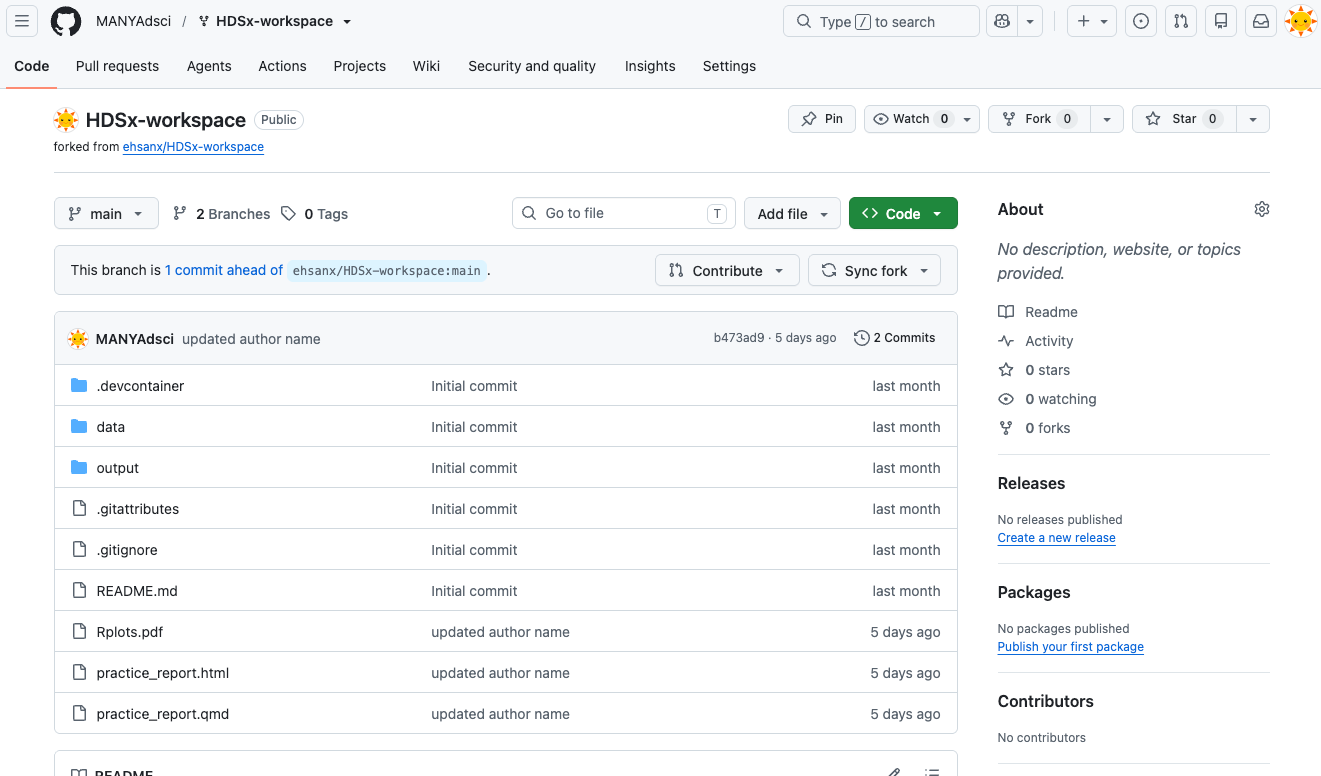
\includegraphics[keepaspectratio]{weeks/week02-modern-workflows/../../assets/images/workflow1/github.png}}

  }

  \caption{The code will be stored and accessible on GitHub as long as
  the company exists. Given that it's owned by a large corporation like
  Microsoft, it will likely last for a long time.}

  \end{figure}%
\item
  Safe if your computer crashes
\item
  This is your \textbf{master copy}
\end{itemize}

\section{Codespace (Public Computer)}\label{codespace-public-computer}

Codespaces is like a library computer:

\begin{itemize}
\item
  \textbf{Temporary machine} It is a disposable environment. If it
  breaks, we just delete it and get a new one.

  \begin{figure}[H]

  {\centering \pandocbounded{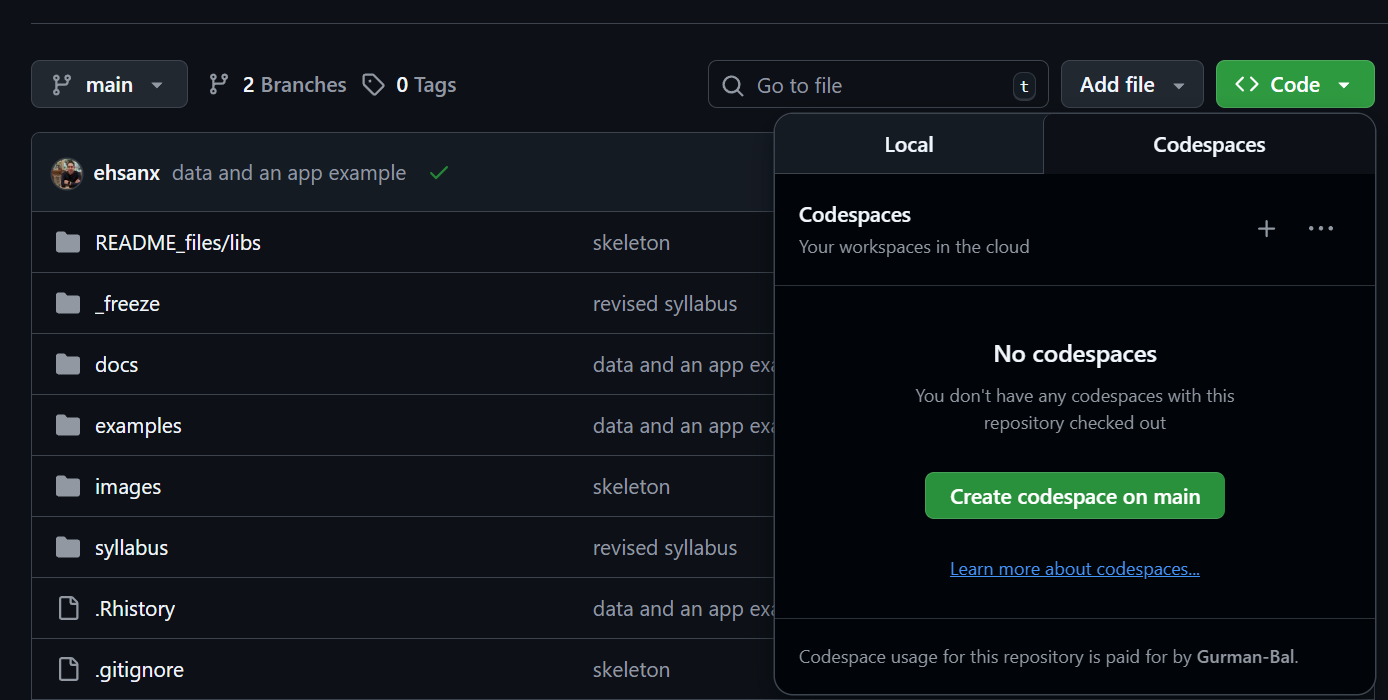
\includegraphics[keepaspectratio]{weeks/week02-modern-workflows/../../assets/images/workflow1/codespace1.png}}

  }

  \caption{Can be accessed by clicking the
  \texttt{\textless{}\textgreater{}\ Code} button, navigating to the
  Codespaces tab, and then starting up a Codespace which contains all
  the file in the Repo.}

  \end{figure}%
\item
  \textbf{Pre-installed software} It comes with R, Python, and Quarto
  installed, so you don't have to install anything on your own laptop.
\item
  \textbf{The ``Two-Save'' Rule (Crucial)} Because this is a temporary
  computer, there are two steps to saving:

  \begin{enumerate}
  \def\labelenumi{\arabic{enumi}.}
  \tightlist
  \item
    \textbf{Ctrl+S (Save):} This only saves to the temporary machine. If
    the machine times out (closes), this is lost.
  \item
    \textbf{Commit \& Push:} This sends your work back to the Repository
    (Cloud Drive). This is the only way to be safe.
  \end{enumerate}
\end{itemize}

\textbf{Warning:} If you close the tab without ``Committing'' (Sending),
your work is erased.

\subsection{Check for understanding}\label{check-for-understanding}

Answer:

\begin{itemize}
\tightlist
\item
  Where are your permanent files stored?
\item
  What happens if you press \texttt{Ctrl+S} but never commit?
\end{itemize}

\chapter{Tour of the Repository}\label{tour-of-the-repository}

\section{Step-by-step}\label{step-by-step}

\begin{enumerate}
\def\labelenumi{\arabic{enumi}.}
\item
  Open your forked course repository on GitHub\\

  \begin{figure}[H]

  {\centering \pandocbounded{
\includegraphics[keepaspectratio]{weeks/week02-modern-workflows/../../assets/images/workflow2/github.png}}

  }

  \caption{Main github page}

  \end{figure}%
\item
  Click the \textbf{Code} tab\\
  \pandocbounded{\includegraphics[keepaspectratio]{weeks/week02-modern-workflows/../../assets/images/workflow2/code.png}}

  \begin{itemize}
  \tightlist
  \item
    \textbf{Why?} GitHub has many tabs (Issues, Actions, Settings). The
    \textbf{Code} tab is your ``Reset'' button. If you ever get lost in
    a menu, click this to go back to your files.
  \end{itemize}
\item
  Look at the file list\\
  \pandocbounded{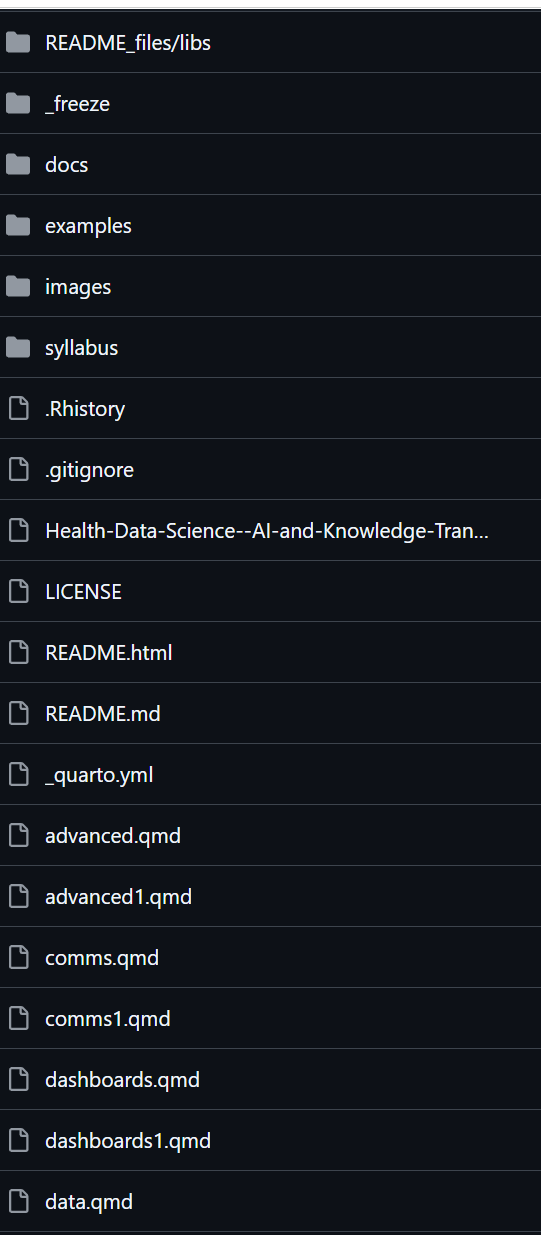
\includegraphics[keepaspectratio]{weeks/week02-modern-workflows/../../assets/images/workflow2/files.png}}

  \begin{itemize}
  \tightlist
  \item
    This shows the \textbf{current state} of the project in your fork.
  \item
    \textbf{Crucial:} If a file is listed here, it is safe. If it is
    \emph{not} here, it only exists on your temporary ``Desk''
    (Codespace) and is at risk of being lost.
  \end{itemize}
\item
  Scroll to read the README

  \begin{itemize}
  \tightlist
  \item
    The \texttt{README.md} file is displayed automatically at the
    bottom. Think of it as the ``Cover Sheet'' or ``Instruction Manual''
    for your project.
  \end{itemize}
\end{enumerate}

\section{Task}\label{task-1}

Find this file:

\begin{verbatim}
practice_report.qmd
\end{verbatim}

\textbf{Verification:} If you can see \texttt{practice\_report.qmd} in
this list, it means the file is safely stored in the cloud (The Vault).

If you can see it in your fork, it is safely stored in the cloud.

\chapter{Opening Your First
Codespace}\label{opening-your-first-codespace}

This process is like walking into the library and turning on a computer.
Start from your forked repository, then create a fresh, temporary
environment in the cloud.

\section{Steps}\label{steps}

\begin{enumerate}
\def\labelenumi{\arabic{enumi}.}
\item
  Click the green \textbf{Code} button

  \begin{itemize}
  \tightlist
  \item
    This button is usually for downloading files, but we are using it to
    launch a computer.
  \end{itemize}

  \begin{figure}[H]

  {\centering \pandocbounded{\includegraphics[keepaspectratio]{weeks/week02-modern-workflows/../../assets/images/workflow3/code.png}}

  }

  \caption{Code button}

  \end{figure}%
\item
  Click the \textbf{Codespaces} tab

  \begin{itemize}
  \tightlist
  \item
    \textbf{Crucial Choice:} You will see two tabs: ``Local'' and
    ``Codespaces.''
  \item
    \textbf{Local:} Means downloading to your own messy laptop (Hard
    mode).
  \item
    \textbf{Codespaces:} Means using the pre-installed cloud computer
    (Easy mode). Always choose this.
  \end{itemize}

  \begin{figure}[H]

  {\centering \pandocbounded{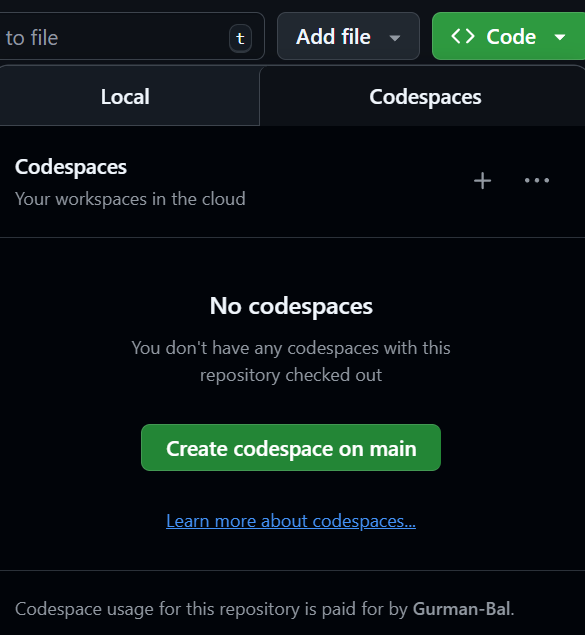
\includegraphics[keepaspectratio]{weeks/week02-modern-workflows/../../assets/images/workflow3/codespaces.png}}

  }

  \caption{Codespaces tab}

  \end{figure}%
\item
  Click \textbf{Create Codespace on main}

  \begin{itemize}
  \tightlist
  \item
    This tells GitHub to build a new computer for you from scratch.
  \end{itemize}

  \begin{figure}[H]

  {\centering \pandocbounded{
\includegraphics[keepaspectratio]{weeks/week02-modern-workflows/../../assets/images/workflow3/create.png}}

  }

  \caption{Create Codespace}

  \end{figure}%
\end{enumerate}

\section{The ``Boot Up'' Phase}\label{the-boot-up-phase}

\textbf{Wait 2--3 minutes.}

\begin{itemize}
\tightlist
\item
  \textbf{What is happening?} GitHub is silently installing R, Python,
  Quarto, and all the course libraries for you.
\item
  \textbf{The Analogy:} Think of this as the ``ventilation system''
  starting up in a lab. It takes a moment to get the environment ready.
\end{itemize}

\textbf{Success:} You should see \textbf{VS Code} (a dark-themed code
editor) appear in your browser window.

\chapter{Reopening a Codespace}\label{reopening-a-codespace}

\textbf{The Rule:} Do not create a new Codespace each time you log in.

\begin{itemize}
\tightlist
\item
  \textbf{Why?} If you click the green ``Create'' button again, GitHub
  builds a \emph{second} computer.
\item
  \textbf{The Risk:} If you left uncommitted work (Drafts) on ``Computer
  A'' and you start ``Computer B,'' your work will appear lost. It isn't
  lost: it's just on the other computer.
\end{itemize}

To resume exactly where you left off:

\section{Steps}\label{steps-1}

\begin{enumerate}
\def\labelenumi{\arabic{enumi}.}
\item
  Go to the \textbf{Codespace Dashboard}:
  \url{https://github.com/codespaces}

  \begin{itemize}
  \tightlist
  \item
    Think of this as the ``Front Desk'' where all your active computers
    are listed.
  \end{itemize}
\item
  Find your Codespace

  \begin{itemize}
  \tightlist
  \item
    Look for the box labeled with your course repository name.
  \item
    \textbf{Note:} GitHub gives each Codespace a funny random name
    (e.g., \emph{literate-computing-machine} or
    \emph{glorious-couscous}). This is the name of your rented desk.
  \end{itemize}

  \begin{figure}[H]

  {\centering \pandocbounded{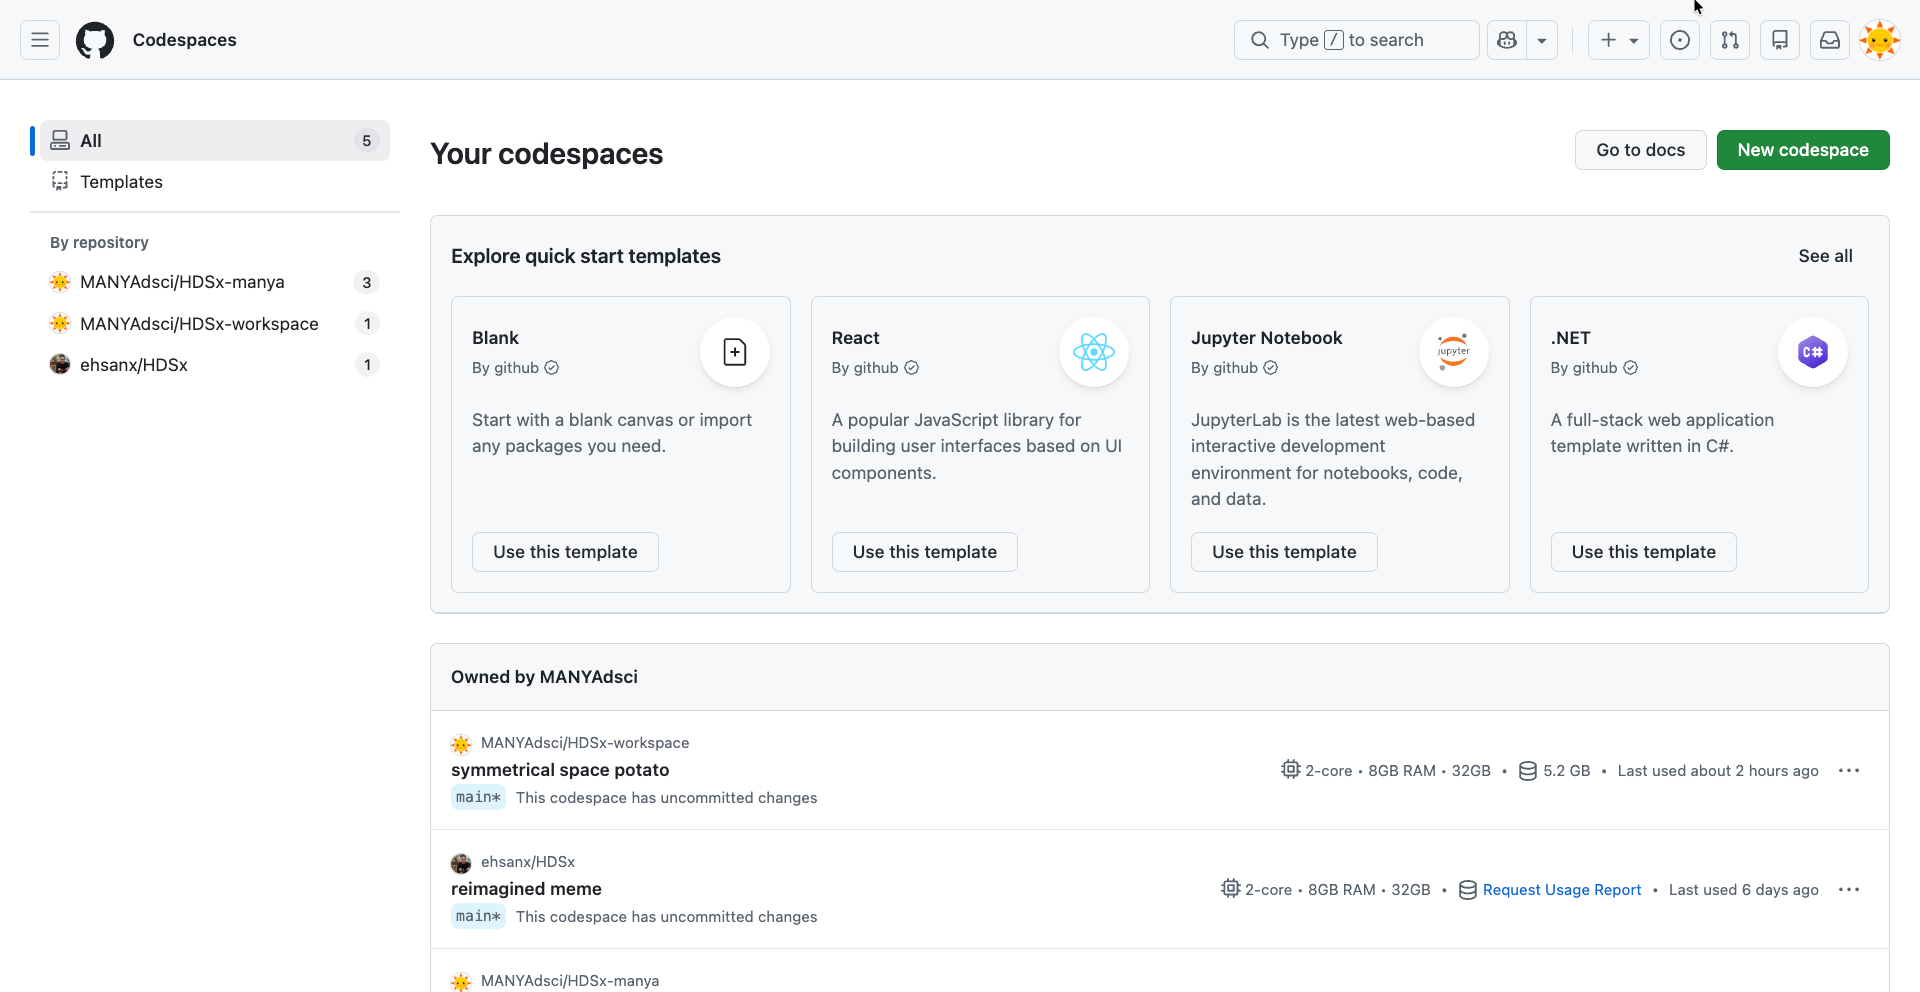
\includegraphics[keepaspectratio]{weeks/week02-modern-workflows/../../assets/images/workflow4/codespace_page.png}}

  }

  \caption{GitHub Codespaces}

  \end{figure}%
\item
  Click the \textbf{Name} of the Codespace

  \begin{itemize}
  \tightlist
  \item
    Do \textbf{not} click the ``New codespace'' button in the corner.
    Click the text link of the funny name.
  \end{itemize}

  \begin{figure}[H]

  {\centering \pandocbounded{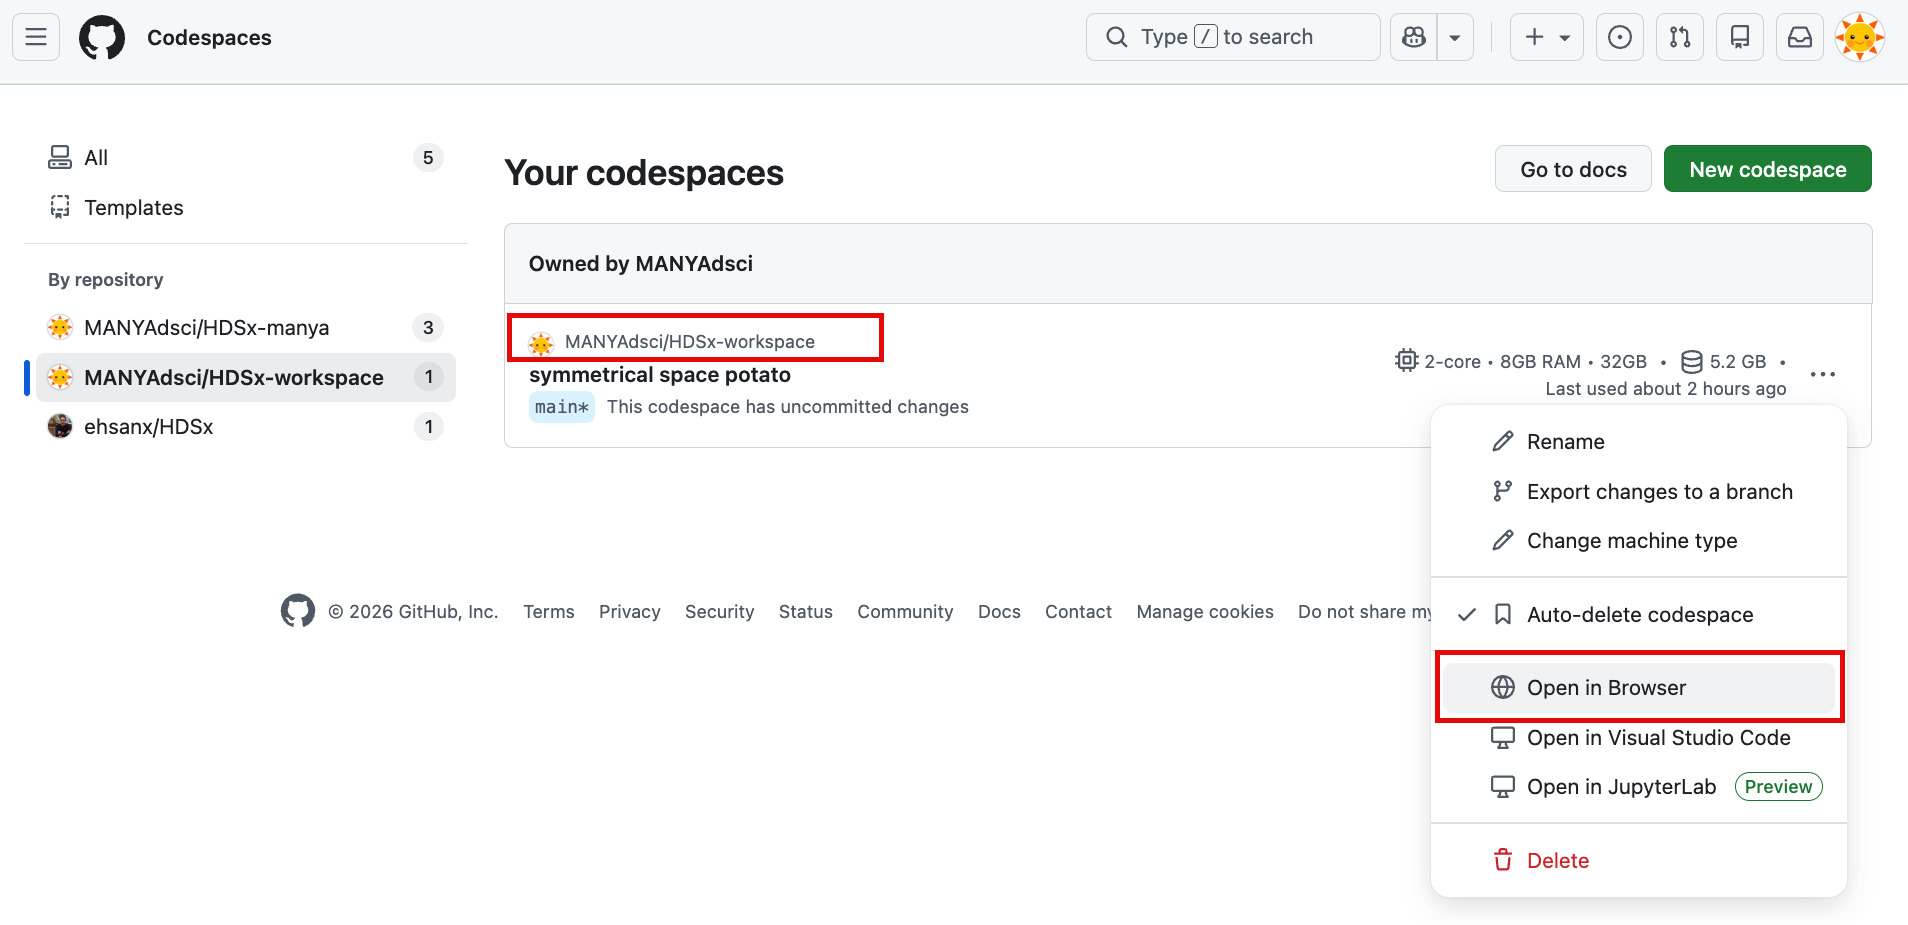
\includegraphics[keepaspectratio]{weeks/week02-modern-workflows/../../assets/images/workflow4/owned.png}}

  }

  \caption{Your Codespace}

  \end{figure}%
\item
  Wait for it to resume

  \begin{itemize}
  \tightlist
  \item
    \textbf{Benefit:} Resuming an existing Codespace is much faster than
    creating a fresh one because the software is already installed.
  \end{itemize}
\end{enumerate}

\chapter{VS Code Orientation}\label{vs-code-orientation}

\pandocbounded{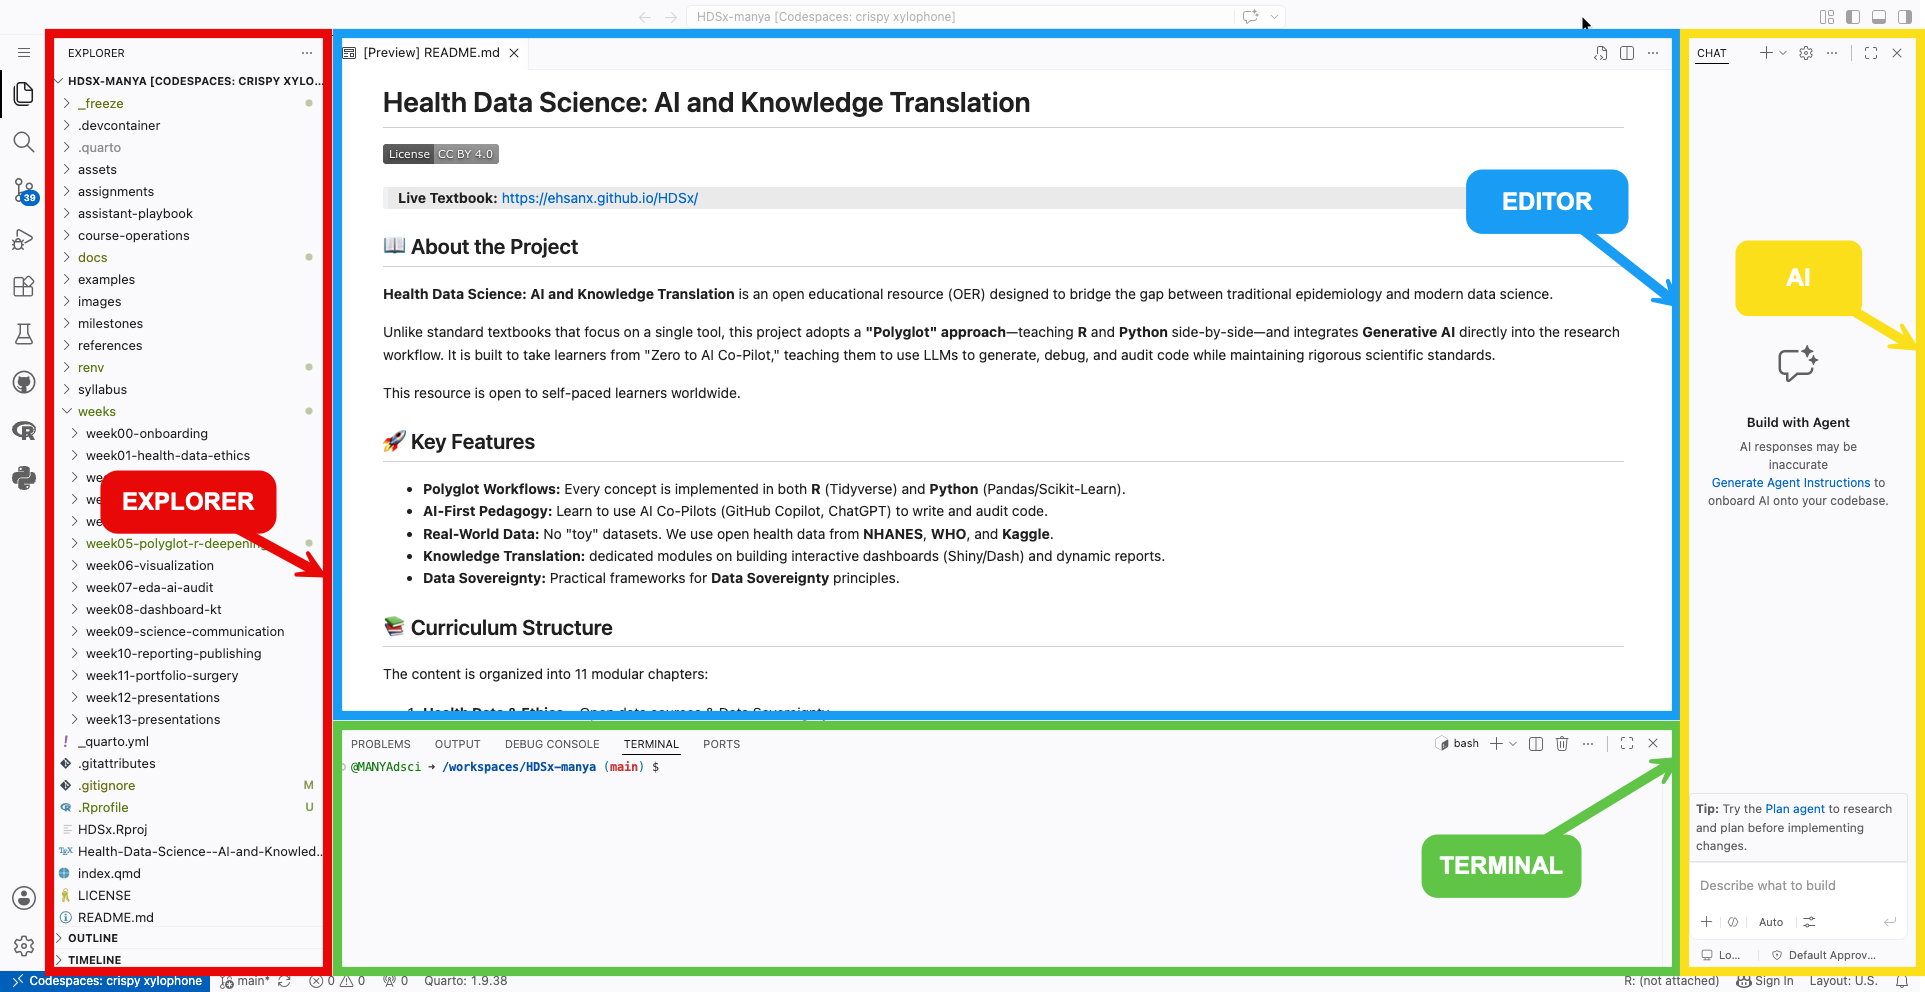
\includegraphics[keepaspectratio]{weeks/week02-modern-workflows/../../assets/images/workflow5/main.png}}

When you open a Codespace, you are using a version of \textbf{VS Code}
in your browser. It has the same interface as the desktop version used
by professional software engineers at Google and Microsoft.

\textbf{Don't Panic:} The interface looks complex because it has
hundreds of features. \textbf{You only need to know three areas.} You
can safely ignore 90\% of the buttons you see.

\section{Explorer (left)}\label{explorer-left}

\textbf{The ``File Cabinet''}

\begin{figure}[H]

{\centering \pandocbounded{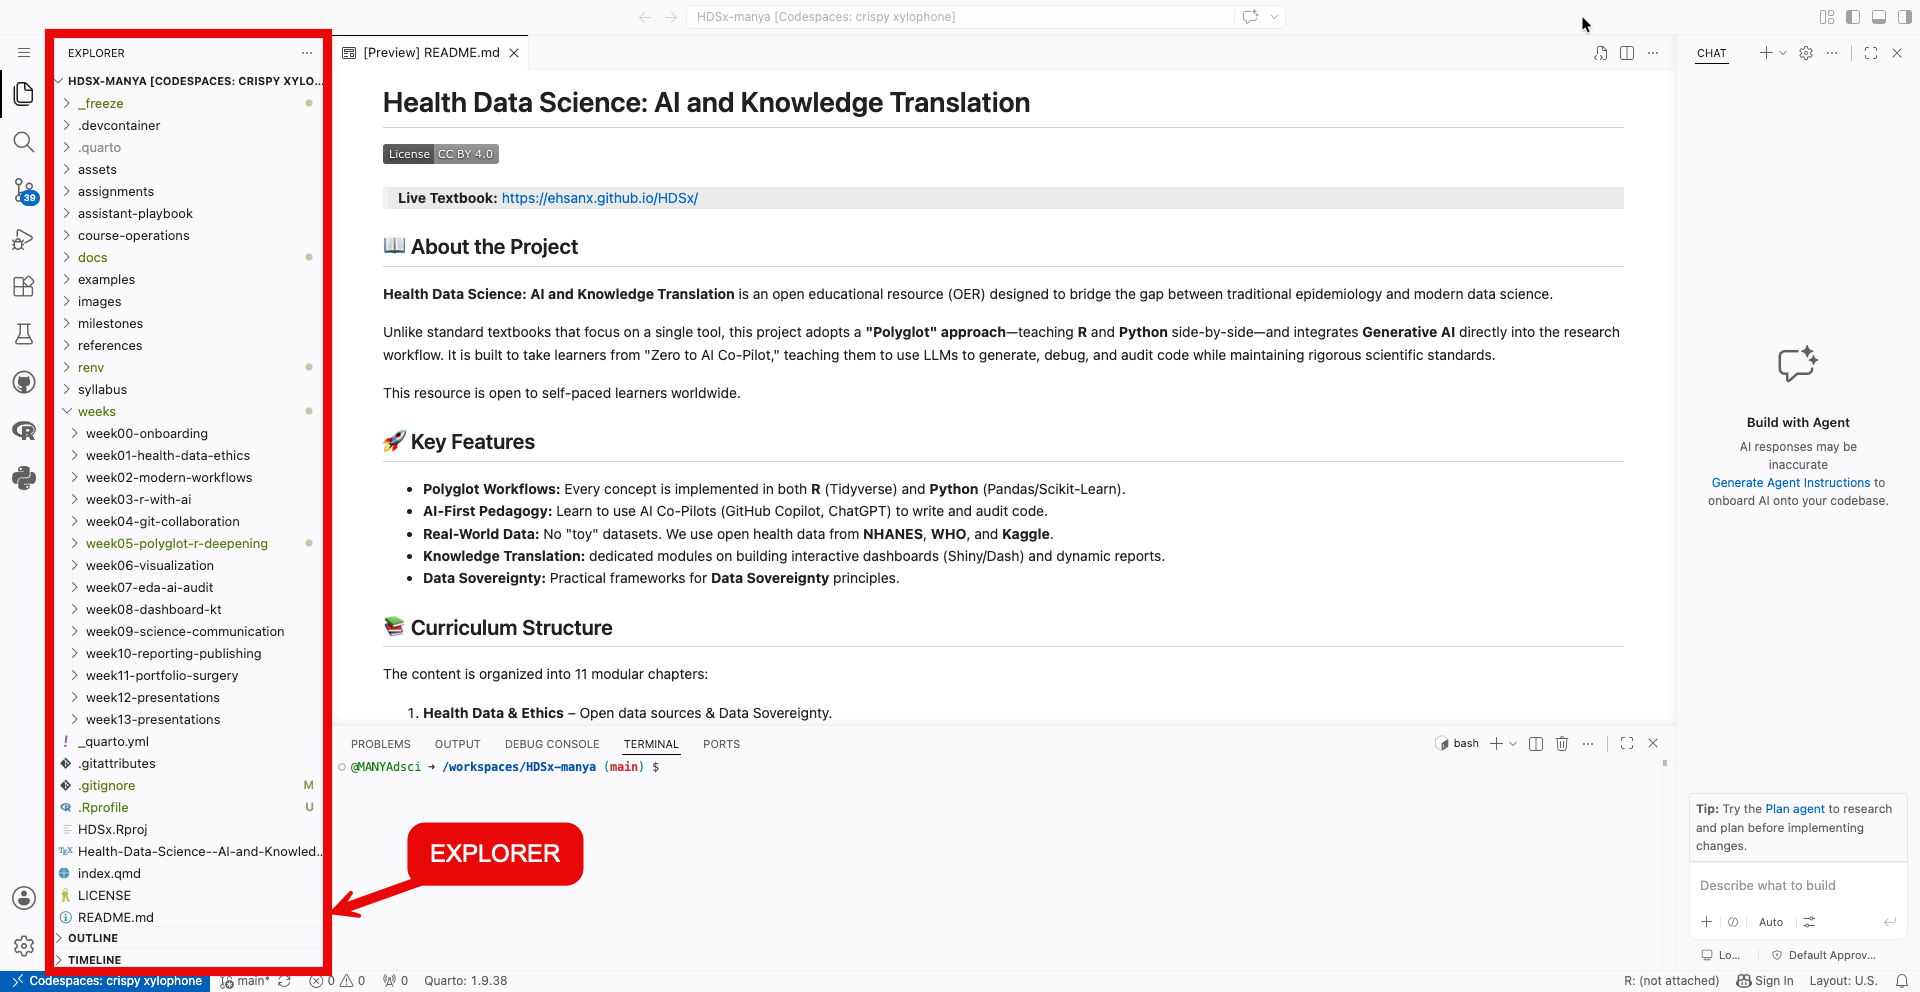
\includegraphics[keepaspectratio]{weeks/week02-modern-workflows/../../assets/images/workflow5/explorer.png}}

}

\caption{Shows files and folders.}

\end{figure}%

\begin{itemize}
\tightlist
\item
  This shows your folders (directories) and files.
\item
  Think of this as your navigation pane. Double-click a file here to
  open it in the Editor.
\end{itemize}

\section{Editor (center)}\label{editor-center}

\textbf{The ``Notebook''}

\begin{figure}[H]

{\centering \pandocbounded{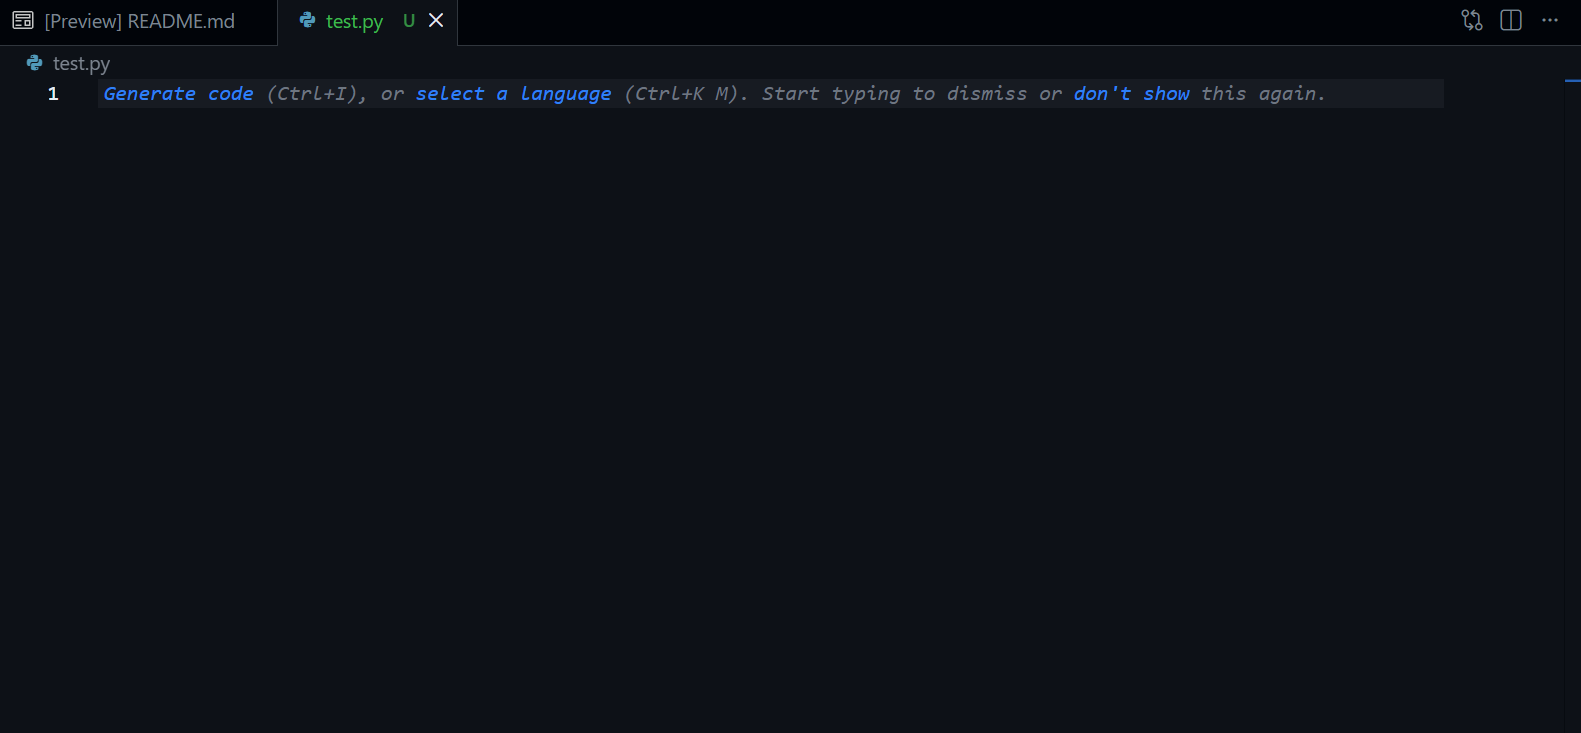
\includegraphics[keepaspectratio]{weeks/week02-modern-workflows/../../assets/images/workflow5/editor.png}}

}

\caption{Where you type.}

\end{figure}%

\begin{itemize}
\tightlist
\item
  This is where you do your actual work: typing code and writing text.
\item
  In this course, you will mostly be editing \texttt{.qmd} (Quarto)
  files here.
\end{itemize}

\section{Terminal (bottom)}\label{terminal-bottom}

\textbf{The ``Engine Room''}

\begin{figure}[H]

{\centering \pandocbounded{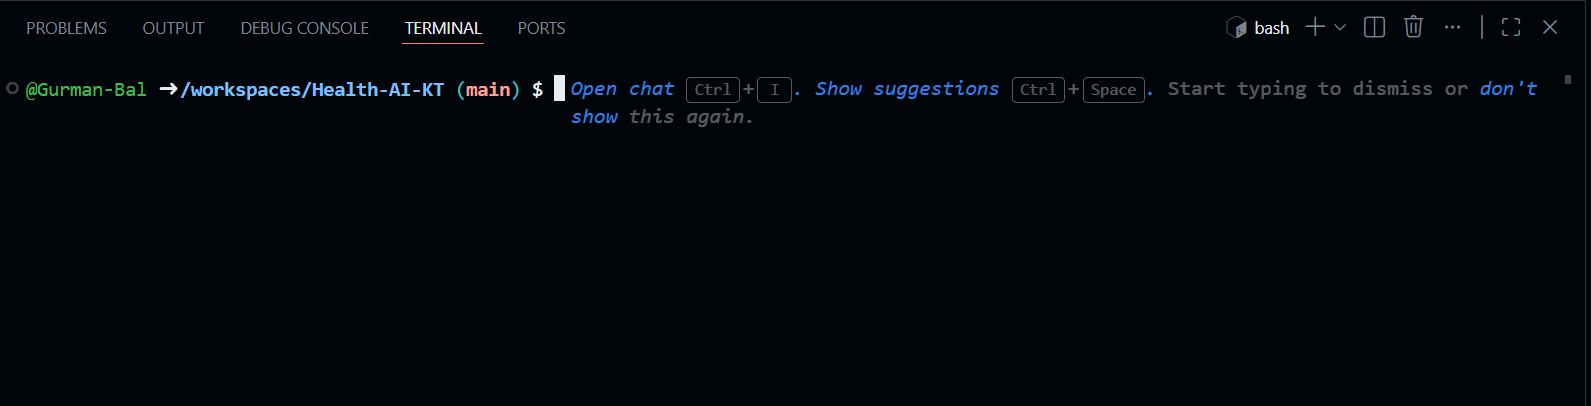
\includegraphics[keepaspectratio]{weeks/week02-modern-workflows/../../assets/images/workflow5/terminal.png}}

}

\caption{Terminal window}

\end{figure}%

\begin{itemize}
\tightlist
\item
  This is where R and Python actually run.
\item
  You will see text scrolling here when you ``Render'' a document. It
  looks like ``The Matrix,'' but it is usually just the computer telling
  you what it is working on.
\end{itemize}

If the terminal disappears (or you accidentally close it):

\textbf{View → Terminal}

\subsection{Mini Task}\label{mini-task}

Open and close a few files in the Explorer to get comfortable with the
layout.

\chapter{Files vs Folders}\label{files-vs-folders}

We use a consistent structure to ensure reproducibility. In Data
Science, being ``organized'' isn't just about being neat---it is a
requirement for your code to work on someone else's machine.

\section{The Golden Rule of Health
Data}\label{the-golden-rule-of-health-data}

We treat data like a \textbf{Crime Scene}---never touch the evidence.

\begin{itemize}
\tightlist
\item
  \textbf{Start:} \texttt{data/} (The Crime Scene). \textbf{READ ONLY.}

  \begin{itemize}
  \tightlist
  \item
    \emph{Rule:} Never open a dataset in Excel and ``fix'' a typo. That
    is tampering with evidence.
  \item
    \emph{Correct Way:} Load the ``dirty'' data into R/Python and fix
    the typo using code. This leaves a trail of exactly what you
    changed.
  \end{itemize}
\item
  \textbf{End:} \texttt{output/} (The Evidence). All graphs and cleaned
  tables go here.
\item
  \textbf{The Detective:} Your code (\texttt{.qmd}) moves information
  from Start to End.
\end{itemize}

\section{Files vs.~Folders (The Mental
Model)}\label{files-vs.-folders-the-mental-model}

\begin{itemize}
\tightlist
\item
  \textbf{Files (e.g., \texttt{report.qmd}):} These are \textbf{sheets
  of paper}. You write on them.
\item
  \textbf{Folders (e.g., \texttt{data/}):} These are \textbf{labeled
  boxes}. You store things in them.
\end{itemize}

\section{Create a folder}\label{create-a-folder}

In Explorer:

\begin{enumerate}
\def\labelenumi{\arabic{enumi}.}
\tightlist
\item
  Right-click anywhere in the blank space of the Explorer pane.
  \pandocbounded{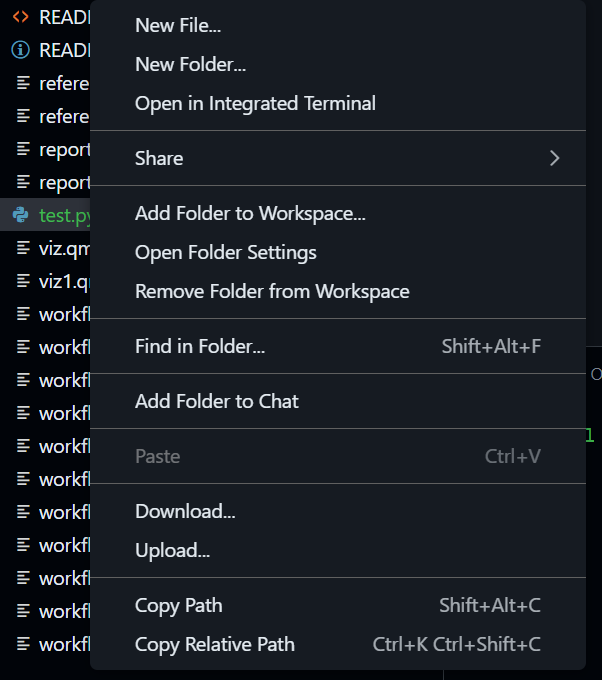
\includegraphics[keepaspectratio]{weeks/week02-modern-workflows/../../assets/images/workflow6/rightclick.png}}
\item
  Select \textbf{New Folder}
\item
  Name it:
\end{enumerate}

\begin{verbatim}
images
\end{verbatim}

\textbf{Pro Tip:} Always use \textbf{lowercase} and \textbf{no spaces}
for folder names (e.g., \texttt{my\_data}, not \texttt{My\ Data}).
Computers struggle with spaces in file paths.

\section{Typical structure}\label{typical-structure}

Your project should always look like this:

\begin{verbatim}
data/      raw data  
output/    generated results  
images/    screenshots  
.qmd       reports  
\end{verbatim}

\textbf{Remember:} The \texttt{data} folder is for \emph{input}. The
\texttt{output} folder is for \emph{results}. They should never mix.

\chapter{The Magic Moment: Render
Quarto}\label{the-magic-moment-render-quarto}

\section{Why do we ``Render''?}\label{why-do-we-render}

In the old days, you would run code, copy a graph, save it as a JPG, and
paste it into Word. If the data changed, you had to redo every step
manually.

\textbf{The Better Way:} Think of your code (\texttt{.qmd} file) as a
\textbf{Recipe} and the final report (HTML/PDF) as the \textbf{Meal}. *
\textbf{Editing:} You don't change the meal; you change the recipe. *
\textbf{Rendering:} This is the ``cooking'' process. When you click
\textbf{Render}, the computer follows your instructions from scratch to
create a fresh meal.

This is the secret to reproducibility: if you give your recipe to a
friend, they can cook the exact same meal.

\section{Step 1 --- Open the file}\label{step-1-open-the-file}

\begin{enumerate}
\def\labelenumi{\arabic{enumi}.}
\tightlist
\item
  Go to the \textbf{Explorer} pane (Left side).
\item
  Locate and click on the file:
\end{enumerate}

\begin{verbatim}
practice_report.qmd
\end{verbatim}

This will open the ``Source Code'' in the center Editor window. You will
see a mix of normal text and code chunks.

\section{Step 2 --- Edit name (The YAML
Header)}\label{step-2-edit-name-the-yaml-header}

Look at the very top of the file. You will see a block of text
sandwiched between three dashes (\texttt{-\/-\/-}). This is called the
\textbf{YAML Header}. It controls the document's metadata.

Find the line that says \texttt{author:}

\begin{verbatim}
author: "Your Name"
\end{verbatim}

\textbf{Task:} Delete ``Your Name'' and type your actual name inside the
quotes. Do not remove the quotes!

\section{Step 3 --- Render}\label{step-3-render}

\begin{enumerate}
\def\labelenumi{\arabic{enumi}.}
\tightlist
\item
  Look for the \textbf{Render} button at the top of the Editor pane (it
  often looks like a Blue Arrow pointing right, or simply says
  ``Render'').
\item
  \textbf{Click it.}
\item
  \textbf{Observe:}

  \begin{itemize}
  \tightlist
  \item
    \textbf{The Terminal (Bottom):} You will see text scrolling quickly.
    This is R/Python executing your code chunks.
  \item
    \textbf{The Preview (Right):} A new window should appear showing a
    beautiful, formatted report with your name on it.
  \end{itemize}
\end{enumerate}

\textbf{Congratulations!} You just performed ``Knowledge
Translation''---turning raw code into a human-readable document.

\section{If it fails
(Troubleshooting)}\label{if-it-fails-troubleshooting}

Rendering involves many moving parts, so it sometimes gets stuck.

\begin{itemize}
\tightlist
\item
  \textbf{The ``Wait'' Rule:} If nothing happens for 20 seconds, the
  background process might be initializing. Give it a moment.
\item
  \textbf{The ``Retry'' Rule:} Sometimes the connection hiccups. Click
  \textbf{Render} one more time.
\item
  \textbf{The ``Red Text'' Rule:} Look at the \textbf{Terminal} tab at
  the bottom. If you see red text, it is an error message. Read it---it
  usually tells you exactly what went wrong (e.g., ``File not found'' or
  ``Syntax error'').
\end{itemize}

\chapter{Commit Your Work}\label{commit-your-work}

Your work is currently only on the ``Rented Desk'' (Codespace). It is a
\textbf{Draft}. To save it permanently to the ``Vault'' (GitHub), you
must \textbf{Commit} and \textbf{Push} (Send).

\textbf{The Analogy:} Think of this like shipping a package. You have
packed the box (saved the file), but now you need to put a label on it
and hand it to the courier.

\section{Steps}\label{steps-2}

\begin{enumerate}
\def\labelenumi{\arabic{enumi}.}
\item
  Click the \textbf{Source Control} icon

  \begin{itemize}
  \tightlist
  \item
    It looks like a \textbf{blue bubble} or a \textbf{connect-the-dots
    graph} on the far left sidebar.
  \item
    This opens the ``Shipping Department.'' You will see a list of every
    file you changed.
  \end{itemize}

  \begin{figure}[H]

  {\centering \pandocbounded{
\includegraphics[keepaspectratio]{weeks/week02-modern-workflows/../../assets/images/workflow8/button.png}}

  }

  \caption{Source control icon circled in red}

  \end{figure}%
\item
  Type a \textbf{Commit Message}

  \begin{itemize}
  \tightlist
  \item
    \textbf{The Label:} You cannot ship a package without a label.
  \item
    \textbf{What to write:} Be descriptive but brief. Imagine you are
    leaving a note for your future self about \emph{what} you did.
  \item
    \emph{Example:} ``Updated author name in practice report''.
  \item
    \emph{Bad Example:} ``stuff'' or ``fix''.
  \end{itemize}

  \begin{figure}[H]

  {\centering \pandocbounded{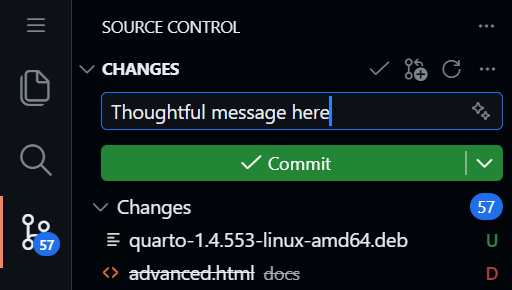
\includegraphics[keepaspectratio]{weeks/week02-modern-workflows/../../assets/images/workflow8/message.png}}

  }

  \caption{This is required}

  \end{figure}%
\item
  Click \textbf{Commit and Sync} (or Commit and Push)

  \begin{itemize}
  \tightlist
  \item
    This is the \textbf{``Send''} button.
  \item
    \textbf{Action:} It wraps up your changes, stamps them with the time
    and your message, and teleports them to the Cloud Vault.
  \item
    \emph{Note:} You might be asked to click ``Always'' or ``Yes'' to
    approve the sync.
  \end{itemize}

  \begin{figure}[H]

  {\centering \pandocbounded{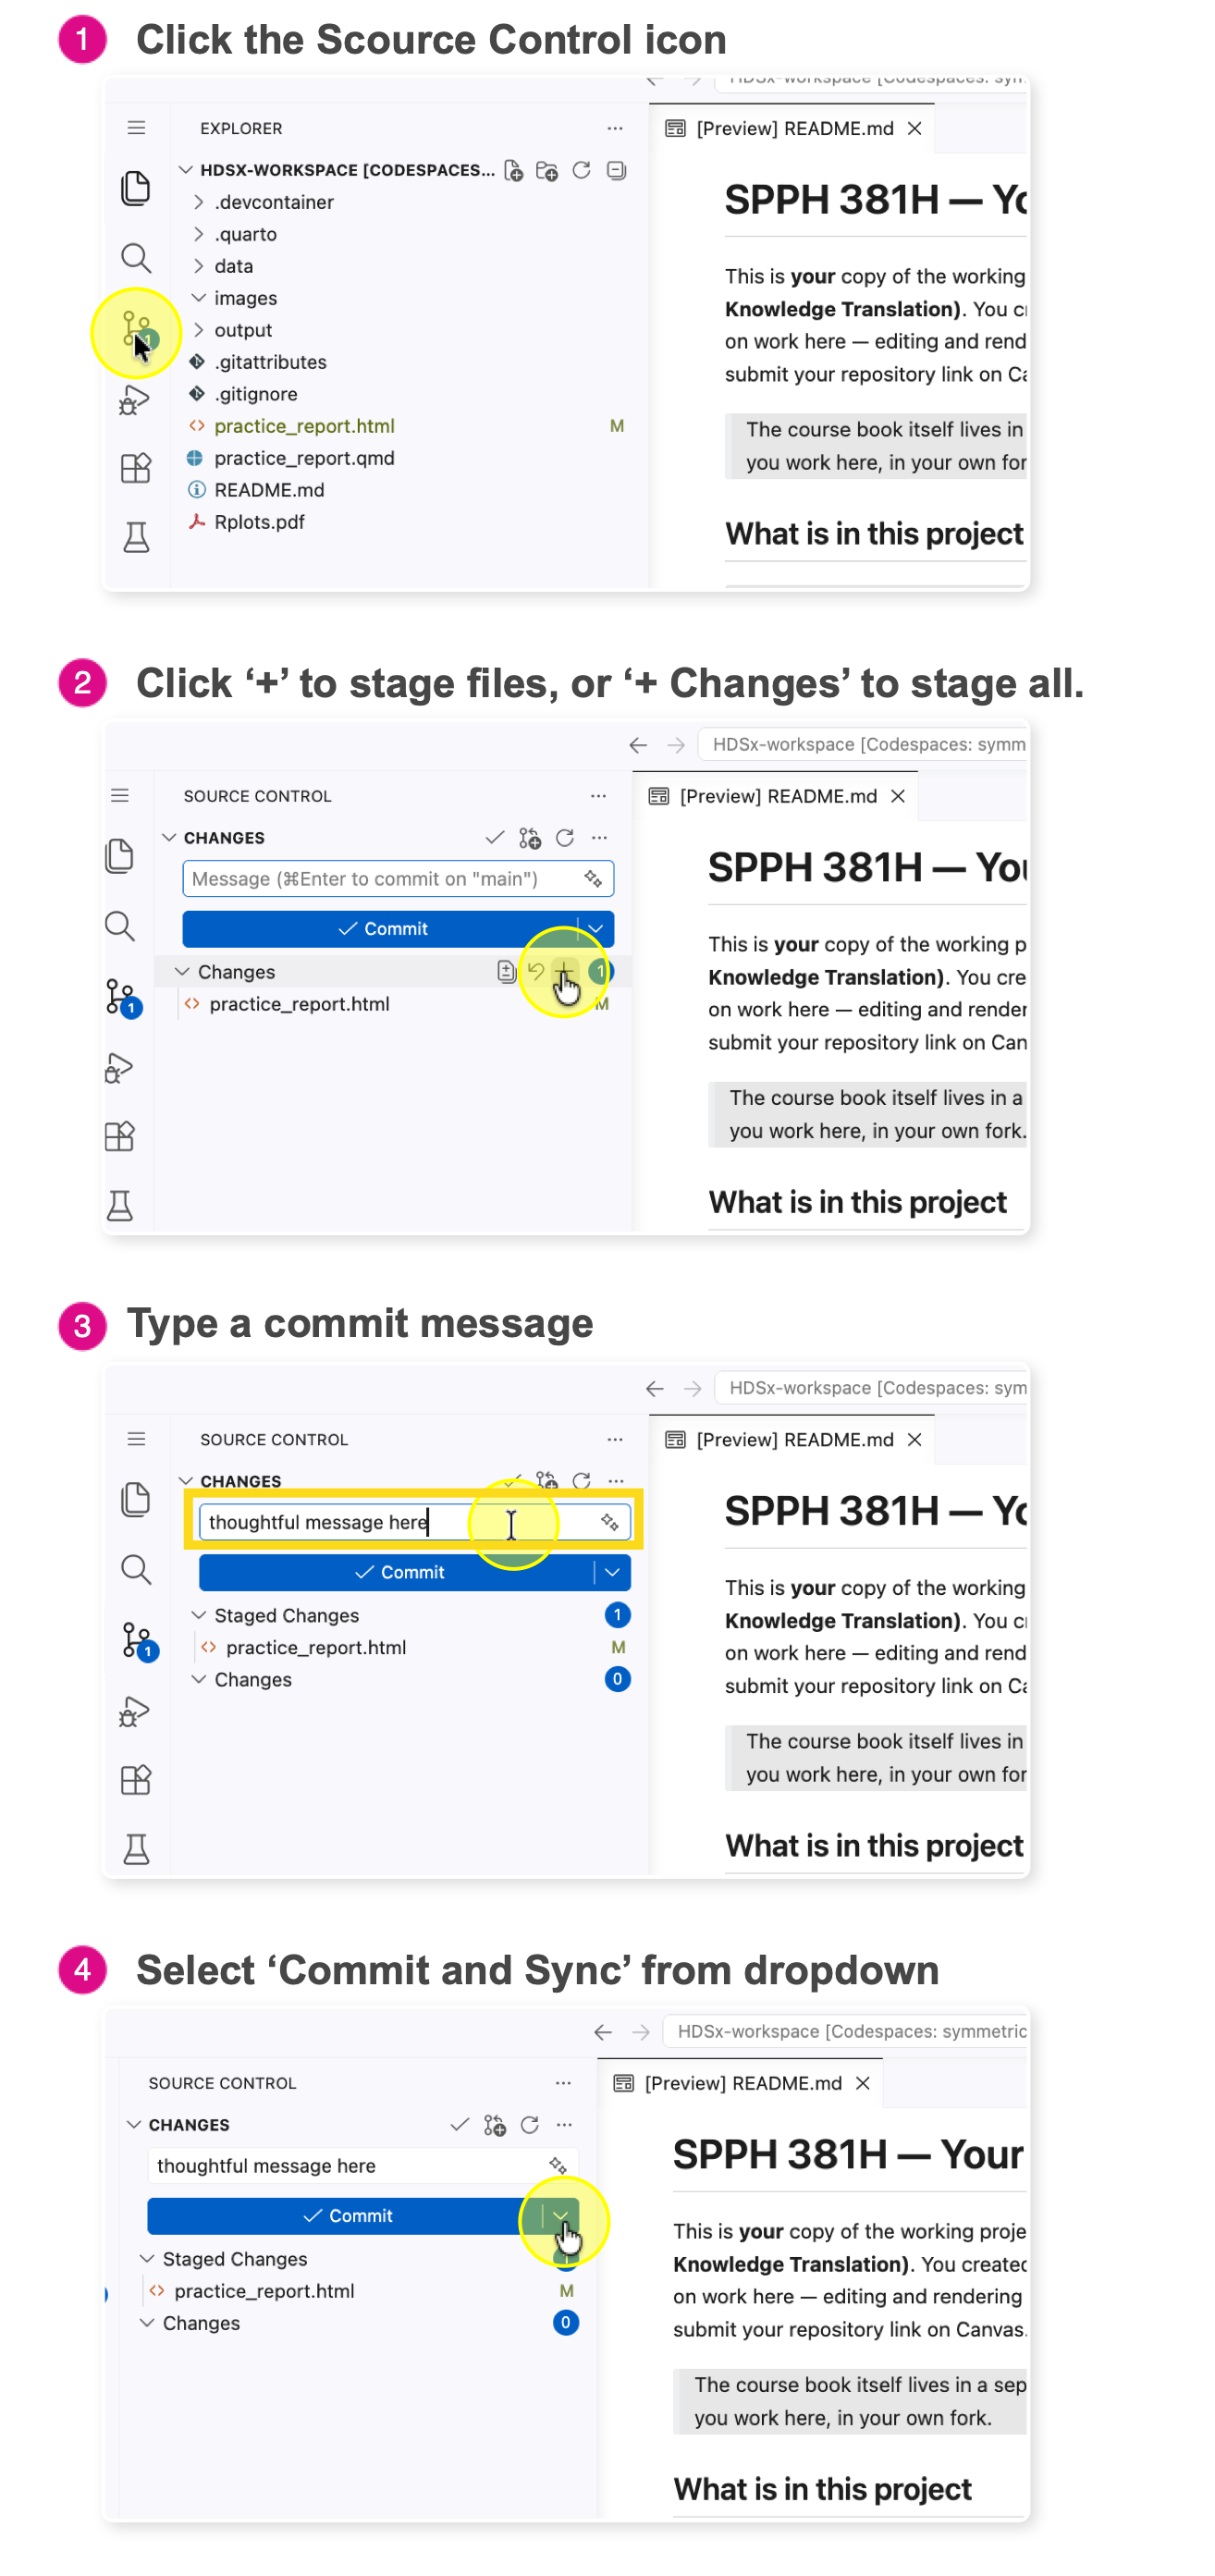
\includegraphics[keepaspectratio]{weeks/week02-modern-workflows/../../assets/images/workflow8/commitpush.png}}

  }

  \caption{This will push your changes to the remote branch}

  \end{figure}%
\end{enumerate}

\section{Verify (Trust but Verify)}\label{verify-trust-but-verify}

Did it actually work?

\begin{enumerate}
\def\labelenumi{\arabic{enumi}.}
\tightlist
\item
  Go back to your \textbf{GitHub Repository} tab (The Vault).
\item
  \textbf{Refresh} the page.
\item
  Look at the file list. You should see your ``Commit Message''
  displayed next to the file you just edited.
\end{enumerate}

\chapter{Troubleshooting: Rebuild
Container}\label{troubleshooting-rebuild-container}

Sometimes the cloud computer gets ``stuck.'' Maybe the terminal froze,
or R crashed.

\textbf{The Fix:} We don't fix broken computers; we get new ones.
``Rebuilding the Container'' is the cloud equivalent of \textbf{``Have
you tried turning it off and on again?''}---but better, because it gives
you a fresh machine while keeping your files safe.

\section{When to use this?}\label{when-to-use-this}

If things break:

\begin{itemize}
\tightlist
\item
  \textbf{Terminal frozen:} You type, but nothing appears.
\item
  \textbf{Render fails:} You get weird errors that make no sense.
\item
  \textbf{Environment issues:} R or Python can't find a package that was
  there yesterday.
\end{itemize}

\section{Steps}\label{steps-3}

\begin{enumerate}
\def\labelenumi{\arabic{enumi}.}
\tightlist
\item
  \textbf{Open the Command Palette}

  \begin{itemize}
  \tightlist
  \item
    Press \texttt{F1} (or \texttt{Ctrl+Shift+P} on Windows /
    \texttt{Cmd+Shift+P} on Mac).
  \item
    A search bar will appear at the very top of the screen. This is the
    ``God Mode'' search bar for VS Code.
  \end{itemize}
\item
  \textbf{Search}

  \begin{itemize}
  \tightlist
  \item
    Type: \texttt{Rebuild\ Container}
  \end{itemize}
\item
  \textbf{Execute}

  \begin{itemize}
  \tightlist
  \item
    Click on the option that says: \textbf{Codespaces: Rebuild
    Container}
  \end{itemize}
\item
  \textbf{Wait (\textasciitilde2-5 minutes)}

  \begin{itemize}
  \tightlist
  \item
    The screen will reload.
  \item
    \textbf{Don't Panic:} You might see a black screen with scrolling
    text logs. This is normal: it is reinstalling the software.
  \item
    When your files reappear in the Explorer, you are ready to go.
  \end{itemize}
\end{enumerate}

\textbf{Did I lose my work?}

\begin{itemize}
\item
  \textbf{Saved files:} No.~Anything you pressed \texttt{Ctrl+S} on is
  safe.
\item
  \textbf{Unsaved typing:} Yes.
\item
  \textbf{R Memory:} Yes. You will need to re-run your code chunks from
  the top.
\end{itemize}

\chapter{Stop Your Codespace}\label{stop-your-codespace}

Codespaces is not free forever. You have a monthly allowance (approx. 60
hours/month for free accounts).

\textbf{The Analogy:} Think of a Codespace like a \textbf{Taxi}.

\begin{itemize}
\tightlist
\item
  \textbf{Working:} When you are coding, the meter is running.
\item
  \textbf{The Trap:} If you just close your browser tab, it is like
  getting out of the taxi but asking the driver to ``wait here.''
  \textbf{The meter keeps running.}
\item
  \textbf{The Fix:} You must explicitly ``end the ride'' (Stop the
  Codespace).
\end{itemize}

\section{Correct shutdown}\label{correct-shutdown}

\begin{enumerate}
\def\labelenumi{\arabic{enumi}.}
\tightlist
\item
  Go to the \textbf{Codespace Dashboard}:
  \url{https://github.com/codespaces}

  \begin{itemize}
  \tightlist
  \item
    This is your command center.
  \end{itemize}
\item
  Find your active Codespace

  \begin{itemize}
  \tightlist
  \item
    Look for the green text that says ``Active''.
  \end{itemize}
\item
  Click \texttt{...} (The ``Meatball'' Menu)

  \begin{itemize}
  \tightlist
  \item
    It is located on the far right side of the Codespace box.
  \end{itemize}
\item
  Click \textbf{Stop Codespace}

  \begin{itemize}
  \tightlist
  \item
    \textbf{Stop:} This ``pauses'' the computer. It saves your installed
    packages and RAM state so you can resume quickly next time.
    \textbf{(Recommended)}
  \item
    \textbf{Delete:} This destroys the computer. You will have to wait
    2-3 minutes for the ``Boot Up'' phase next time you start.
  \end{itemize}
\end{enumerate}

\textbf{Critical Warning:} Closing the browser tab is \textbf{NOT}
enough.

\begin{itemize}
\item
  GitHub keeps the machine running for \textbf{30 minutes} after you
  close the tab (in case your internet flickered).
\item
  \textbf{The Cost:} If you just close the tab every day, you will waste
  \textasciitilde15 hours of your monthly quota on empty time.
\end{itemize}

\pandocbounded{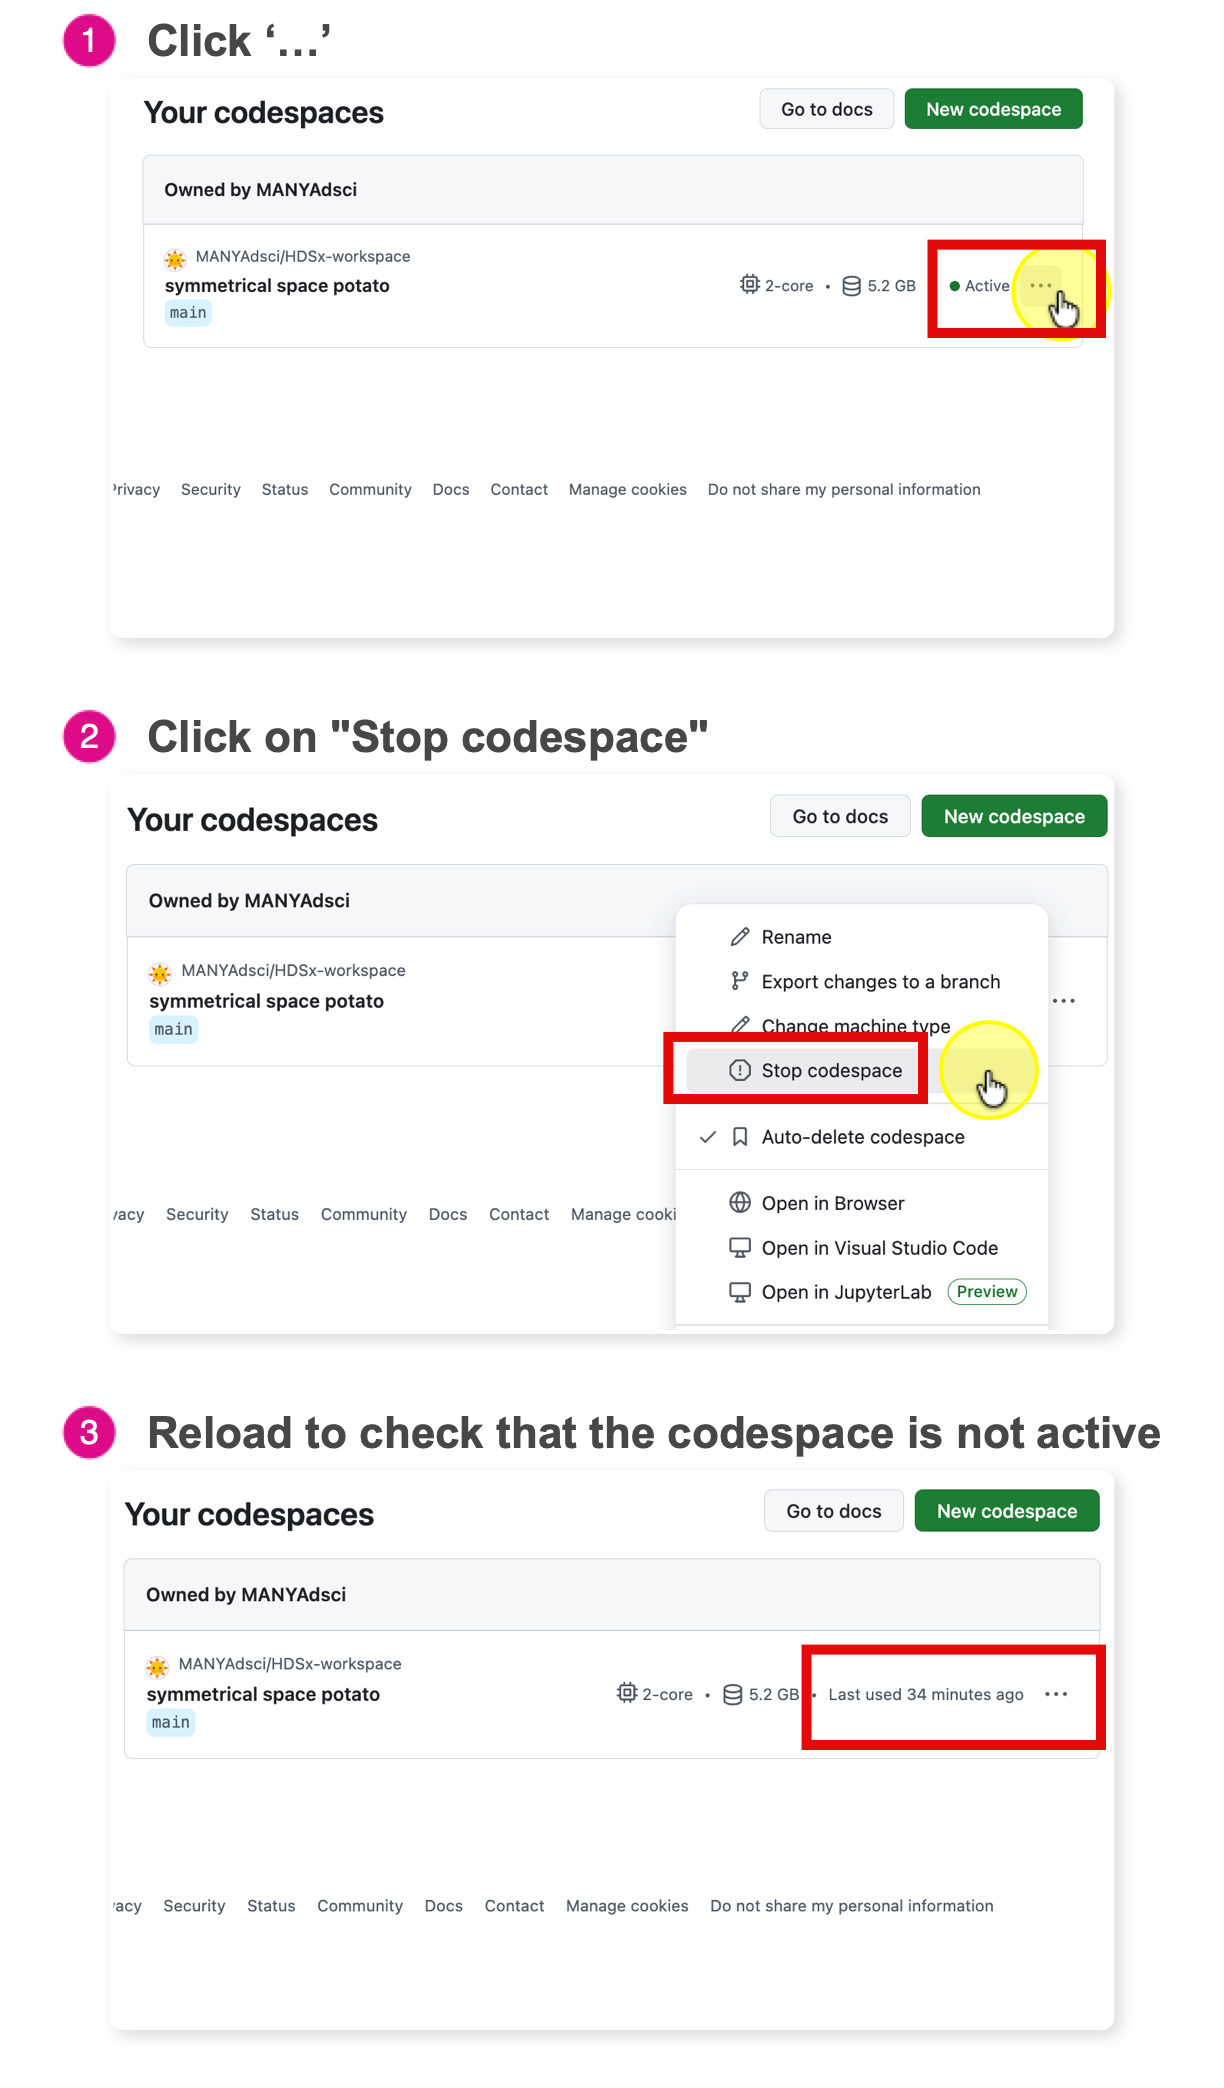
\includegraphics[keepaspectratio]{weeks/week02-modern-workflows/../../assets/images/workflow10/stop.png}}

\chapter{Final Checklist}\label{final-checklist}

\begin{itemize}
\tightlist
\item[$\square$]
  I understand repository vs Codespace\\
\item[$\square$]
  I created or located my forked course repository\\
\item[$\square$]
  I rendered a \texttt{.qmd} file\\
\item[$\square$]
  I committed changes\\
\item[$\square$]
  I know how to rebuild container\\
\item[$\square$]
  I know how to stop Codespace
\end{itemize}

\section{Reflection}\label{reflection}

Write 2--3 sentences:

\begin{itemize}
\tightlist
\item
  What was easiest?
\item
  What was confusing?
\item
  What questions do you still have?
\end{itemize}

\part{Week 3: R with AI}

\chapter*{Week 3: R with AI}\label{week-3-r-with-ai-1}
\addcontentsline{toc}{chapter}{Week 3: R with AI}

\markboth{Week 3: R with AI}{Week 3: R with AI}

\section*{Overview}\label{overview-2}
\addcontentsline{toc}{section}{Overview}

\markright{Overview}

\textbf{Summary:} In Week 2 you learned how to use your Codespace, edit
a Quarto document, and make your first commit. Now you learn how to
speak R---not by memorizing syntax, but by directing an AI co-pilot and
\emph{auditing} what it writes. Your job is to be the pilot: you decide
what the analysis should do, the AI drafts the code, and you verify
every line before it flies.

\textbf{Learning Objectives:}

\begin{itemize}
\tightlist
\item
  Understand that R is a calculator that needs specific, case-sensitive
  instructions.
\item
  Load packages with \texttt{library()} and explain why this is needed
  each session.
\item
  Run a minimal \texttt{renv} checkpoint so package changes are visible.
\item
  Use core constructs: variables (assignment), functions (with
  arguments), and the pipe (\texttt{\%\textgreater{}\%} /
  \texttt{\textbar{}\textgreater{}}).
\item
  Perform basic data transformations using \texttt{dplyr} verbs:
  \texttt{filter()}, \texttt{select()}, \texttt{mutate()},
  \texttt{summarise()}, \texttt{group\_by()}.
\item
  Inspect a dataset on first contact: structure, dimensions,
  missingness.
\item
  Identify control flow (\texttt{if/else}, loops) in AI-generated code
  and audit whether it is correct.
\item
  Write and adapt a simple custom function.
\item
  Apply an AI safety checklist to catch hallucinations, wrong column
  names, and unsafe operations.
\item
  Document your analysis in Quarto by weaving code chunks with Markdown
  narrative.
\item
  Commit incrementally as you work (reinforcing Week 2 Git basics).
\end{itemize}

\section*{Connection}\label{connection-2}
\addcontentsline{toc}{section}{Connection}

\markright{Connection}

Week 2 made the project structure reproducible. This week you use that
structure to load, inspect, summarize, and audit R code with AI support.
Next week you will put those edits under version control.

\section*{Case Study Data Analysis}\label{case-study-data-analysis}
\addcontentsline{toc}{section}{Case Study Data Analysis}

\markright{Case Study Data Analysis}

The \textbf{NHANES Health Equity data spine} now supports code-reading,
EDA, visualization, and reproducibility checks. Use the cached CSV/RDS
for routine class work; a CDC retrieval script exists for advanced
users.

\begin{itemize}
\tightlist
\item
  Cached RDS:
  \texttt{examples/nhanes-equity/data/nhanes\_equity\_v6.rds}
\item
  CSV snapshot:
  \texttt{examples/nhanes-equity/data/nhanes\_equity\_v6.csv}
\item
  Case-study README: \texttt{examples/nhanes-equity/README.md}
\end{itemize}

The default classroom path is to use the cached data so the analysis
work is reproducible without internet access.

\begin{Shaded}
\begin{Highlighting}[numbers=left,,]
\FunctionTok{library}\NormalTok{(readr)}
\FunctionTok{library}\NormalTok{(dplyr)}

\NormalTok{candidate\_paths }\OtherTok{\textless{}{-}} \FunctionTok{c}\NormalTok{(}
  \StringTok{"examples/nhanes{-}equity/data/nhanes\_equity\_v6.csv"}\NormalTok{,}
  \StringTok{"../../examples/nhanes{-}equity/data/nhanes\_equity\_v6.csv"}
\NormalTok{)}

\NormalTok{nhanes\_path }\OtherTok{\textless{}{-}}\NormalTok{ candidate\_paths[}\FunctionTok{file.exists}\NormalTok{(candidate\_paths)][}\DecValTok{1}\NormalTok{]}
\ControlFlowTok{if}\NormalTok{ (}\FunctionTok{is.na}\NormalTok{(nhanes\_path)) \{}
  \FunctionTok{stop}\NormalTok{(}\StringTok{"Could not find examples/nhanes{-}equity/data/nhanes\_equity\_v6.csv"}\NormalTok{)}
\NormalTok{\}}

\NormalTok{nhanes\_analysis }\OtherTok{\textless{}{-}} \FunctionTok{read\_csv}\NormalTok{(nhanes\_path, }\AttributeTok{show\_col\_types =} \ConstantTok{FALSE}\NormalTok{)}

\NormalTok{nhanes\_analysis }\SpecialCharTok{|\textgreater{}}
  \FunctionTok{summarise}\NormalTok{(}
    \AttributeTok{rows =} \FunctionTok{n}\NormalTok{(),}
    \AttributeTok{missing\_bmi =} \FunctionTok{sum}\NormalTok{(}\FunctionTok{is.na}\NormalTok{(BMI)),}
    \AttributeTok{missing\_income =} \FunctionTok{sum}\NormalTok{(}\FunctionTok{is.na}\NormalTok{(IncomeGroup))}
\NormalTok{  )}
\CommentTok{\#\textgreater{} \# A tibble: 1 x 3}
\CommentTok{\#\textgreater{}     rows missing\_bmi missing\_income}
\CommentTok{\#\textgreater{}    \textless{}int\textgreater{}       \textless{}int\textgreater{}          \textless{}int\textgreater{}}
\CommentTok{\#\textgreater{} 1 105626        9356           9415}

\NormalTok{nhanes\_analysis }\SpecialCharTok{|\textgreater{}}
  \FunctionTok{filter}\NormalTok{(}\SpecialCharTok{!}\FunctionTok{is.na}\NormalTok{(BMI), }\SpecialCharTok{!}\FunctionTok{is.na}\NormalTok{(IncomeGroup), Age }\SpecialCharTok{\textgreater{}=} \DecValTok{20}\NormalTok{, Age }\SpecialCharTok{\textless{}=} \DecValTok{80}\NormalTok{) }\SpecialCharTok{|\textgreater{}}
  \FunctionTok{group\_by}\NormalTok{(IncomeGroup) }\SpecialCharTok{|\textgreater{}}
  \FunctionTok{summarise}\NormalTok{(}
    \AttributeTok{n =} \FunctionTok{n}\NormalTok{(),}
    \AttributeTok{mean\_bmi =} \FunctionTok{round}\NormalTok{(}\FunctionTok{mean}\NormalTok{(BMI), }\DecValTok{1}\NormalTok{),}
    \AttributeTok{.groups =} \StringTok{"drop"}
\NormalTok{  )}
\CommentTok{\#\textgreater{} \# A tibble: 3 x 3}
\CommentTok{\#\textgreater{}   IncomeGroup            n mean\_bmi}
\CommentTok{\#\textgreater{}   \textless{}chr\textgreater{}              \textless{}int\textgreater{}    \textless{}dbl\textgreater{}}
\CommentTok{\#\textgreater{} 1 High Income (\textgreater{}3.5) 16330     28.6}
\CommentTok{\#\textgreater{} 2 Low Income (\textless{}1.3)  15293     29.4}
\CommentTok{\#\textgreater{} 3 Middle Income      19228     29.3}
\end{Highlighting}
\end{Shaded}

\section*{In-Class Activity}\label{in-class-activity-2}
\addcontentsline{toc}{section}{In-Class Activity}

\markright{In-Class Activity}

\begin{itemize}
\tightlist
\item
  Load the CSV snapshot and inspect column names, row count, and
  missingness.
\item
  Summarize one numeric variable and one grouping variable with clear
  \texttt{NA} handling.
\item
  Ask an AI assistant to comment on your code, then audit whether the
  comments match the actual operations.
\item
  Note one place where an AI assistant could hallucinate a variable name
  or overstate what the descriptive summary means.
\end{itemize}

Student output: a short Quarto note with one data inspection, one
summary, and one AI-audit comment. Assignment link:
\href{../../assignments/assignment02-r-with-ai/README.md}{Assignment 2}.

\begin{center}\rule{0.5\linewidth}{0.5pt}\end{center}

\section*{\texorpdfstring{\texttt{r1.qmd} Packages: Opening the
Toolbox}{r1.qmd Packages: Opening the Toolbox}}\label{r1.qmd-packages-opening-the-toolbox}
\addcontentsline{toc}{section}{\texttt{r1.qmd} Packages: Opening the
Toolbox}

\markright{\texttt{r1.qmd} Packages: Opening the Toolbox}

\subsection*{Install vs Load}\label{install-vs-load}
\addcontentsline{toc}{subsection}{Install vs Load}

\begin{itemize}
\tightlist
\item
  \texttt{install.packages("tidyverse")} --- \textbf{buying} the
  toolbox. Done once per environment (already done in your course
  Codespace).
\item
  \texttt{library(tidyverse)} --- \textbf{opening} the toolbox. Required
  every time you restart R or reopen your Codespace.
\end{itemize}

\begin{Shaded}
\begin{Highlighting}[numbers=left,,]
\FunctionTok{library}\NormalTok{(tidyverse)}
\end{Highlighting}
\end{Shaded}

\begin{tcolorbox}[enhanced jigsaw, opacitybacktitle=0.6, colbacktitle=quarto-callout-note-color!10!white, breakable, opacityback=0, coltitle=black, toptitle=1mm, bottomrule=.15mm, colframe=quarto-callout-note-color-frame, bottomtitle=1mm, colback=white, leftrule=.75mm, rightrule=.15mm, title=\textcolor{quarto-callout-note-color}{\faInfo}\hspace{0.5em}{Note}, left=2mm, arc=.35mm, toprule=.15mm, titlerule=0mm]

If you see an error like
\texttt{there\ is\ no\ package\ called\ \textquotesingle{}tidyverse\textquotesingle{}},
the package is not installed in your Codespace. Use the Canvas support
channel or office hours and include the full error message.

\end{tcolorbox}

\subsection*{Minimal renv Checkpoint}\label{minimal-renv-checkpoint}
\addcontentsline{toc}{subsection}{Minimal renv Checkpoint}

\texttt{renv} helps record which R packages a project uses. You do not
need to master \texttt{renv} this week, but you should recognize the
three checkpoint commands that support reproducibility.

\begin{Shaded}
\begin{Highlighting}[numbers=left,,]
\CommentTok{\# Check whether the project environment has changed.}
\NormalTok{renv}\SpecialCharTok{::}\FunctionTok{status}\NormalTok{()}

\CommentTok{\# Record package changes when you intentionally add or update packages.}
\NormalTok{renv}\SpecialCharTok{::}\FunctionTok{snapshot}\NormalTok{()}

\CommentTok{\# Restore the recorded package environment in a fresh setup.}
\NormalTok{renv}\SpecialCharTok{::}\FunctionTok{restore}\NormalTok{()}
\end{Highlighting}
\end{Shaded}

For Assignment 2, run \texttt{renv::status()} and write a short
dependency note. Only run \texttt{renv::snapshot()} if you intentionally
added a package.

\begin{center}\rule{0.5\linewidth}{0.5pt}\end{center}

\section*{\texorpdfstring{\texttt{r2.qmd} Core Constructs: Boxes,
Toasters, and the Assembly
Line}{r2.qmd Core Constructs: Boxes, Toasters, and the Assembly Line}}\label{r2.qmd-core-constructs-boxes-toasters-and-the-assembly-line}
\addcontentsline{toc}{section}{\texttt{r2.qmd} Core Constructs: Boxes,
Toasters, and the Assembly Line}

\markright{\texttt{r2.qmd} Core Constructs: Boxes, Toasters, and the
Assembly Line}

\subsection*{Variables: The Labeled
Box}\label{variables-the-labeled-box}
\addcontentsline{toc}{subsection}{Variables: The Labeled Box}

R has no memory unless you store results in a named box using
\texttt{\textless{}-}.

\begin{Shaded}
\begin{Highlighting}[numbers=left,,]
\NormalTok{patient\_age }\OtherTok{\textless{}{-}} \DecValTok{55}
\NormalTok{clinic\_name }\OtherTok{\textless{}{-}} \StringTok{"Vancouver General"}
\end{Highlighting}
\end{Shaded}

\begin{tcolorbox}[enhanced jigsaw, opacitybacktitle=0.6, colbacktitle=quarto-callout-warning-color!10!white, breakable, opacityback=0, coltitle=black, toptitle=1mm, bottomrule=.15mm, colframe=quarto-callout-warning-color-frame, bottomtitle=1mm, colback=white, leftrule=.75mm, rightrule=.15mm, title=\textcolor{quarto-callout-warning-color}{\faExclamationTriangle}\hspace{0.5em}{Warning}, left=2mm, arc=.35mm, toprule=.15mm, titlerule=0mm]

\textbf{Case sensitivity:} \texttt{Age}, \texttt{age}, and \texttt{AGE}
are three different boxes. This is one of the most common bugs in
AI-generated code. Always check that column names match your data
exactly.

\end{tcolorbox}

\subsection*{Functions: The Toaster}\label{functions-the-toaster}
\addcontentsline{toc}{subsection}{Functions: The Toaster}

A function takes \textbf{input} and returns \textbf{output}. Arguments
(inside the parentheses) control its behaviour.

\begin{Shaded}
\begin{Highlighting}[numbers=left,,]
\FunctionTok{mean}\NormalTok{(}\FunctionTok{c}\NormalTok{(}\DecValTok{72}\NormalTok{, }\DecValTok{85}\NormalTok{, }\DecValTok{90}\NormalTok{), }\AttributeTok{na.rm =} \ConstantTok{TRUE}\NormalTok{)}
\end{Highlighting}
\end{Shaded}

\begin{itemize}
\tightlist
\item
  \texttt{c(72,\ 85,\ 90)} is the input (a vector of numbers).
\item
  \texttt{na.rm\ =\ TRUE} tells R to ignore missing values.
  \textbf{Always look for this} when auditing AI code that works with
  health data --- missingness is the norm, not the exception.
\end{itemize}

\subsection*{The Pipe: The Assembly
Line}\label{the-pipe-the-assembly-line}
\addcontentsline{toc}{subsection}{The Pipe: The Assembly Line}

The pipe passes the result of one step into the next. Think of it as
\textbf{``and then\ldots{}''}

\begin{Shaded}
\begin{Highlighting}[numbers=left,,]
\NormalTok{data }\SpecialCharTok{\%\textgreater{}\%}
  \FunctionTok{filter}\NormalTok{(age }\SpecialCharTok{\textgreater{}} \DecValTok{65}\NormalTok{) }\SpecialCharTok{\%\textgreater{}\%}
  \FunctionTok{summarise}\NormalTok{(}\AttributeTok{mean\_bmi =} \FunctionTok{mean}\NormalTok{(bmi, }\AttributeTok{na.rm =} \ConstantTok{TRUE}\NormalTok{))}
\end{Highlighting}
\end{Shaded}

Read this as: \emph{``Take the data, and then keep only patients over
65, and then calculate the average BMI.''}

\begin{tcolorbox}[enhanced jigsaw, opacitybacktitle=0.6, colbacktitle=quarto-callout-tip-color!10!white, breakable, opacityback=0, coltitle=black, toptitle=1mm, bottomrule=.15mm, colframe=quarto-callout-tip-color-frame, bottomtitle=1mm, colback=white, leftrule=.75mm, rightrule=.15mm, title=\textcolor{quarto-callout-tip-color}{\faLightbulb}\hspace{0.5em}{Tip}, left=2mm, arc=.35mm, toprule=.15mm, titlerule=0mm]

You will see two pipe symbols in the wild: \texttt{\%\textgreater{}\%}
(from the \texttt{magrittr} / \texttt{tidyverse} packages) and
\texttt{\textbar{}\textgreater{}} (built into R 4.1+). They do the same
thing for our purposes. If AI generates the other one, don't panic ---
both work in your Codespace.

\end{tcolorbox}

\begin{center}\rule{0.5\linewidth}{0.5pt}\end{center}

\section*{\texorpdfstring{\texttt{r3.qmd} Data Import and First
Contact}{r3.qmd Data Import and First Contact}}\label{r3.qmd-data-import-and-first-contact}
\addcontentsline{toc}{section}{\texttt{r3.qmd} Data Import and First
Contact}

\markright{\texttt{r3.qmd} Data Import and First Contact}

\subsection*{Loading Data}\label{loading-data}
\addcontentsline{toc}{subsection}{Loading Data}

Use relative paths so your code runs on any machine (including your
grader's Codespace).

\begin{Shaded}
\begin{Highlighting}[numbers=left,,]
\NormalTok{my\_data }\OtherTok{\textless{}{-}} \FunctionTok{read\_csv}\NormalTok{(}\StringTok{"data/patients.csv"}\NormalTok{)}
\end{Highlighting}
\end{Shaded}

\textbf{How to get the path right:} Right-click the file in the VS Code
Explorer → \textbf{Copy Relative Path} → paste it into your code.

\textbf{AI Prompt:}

\begin{quote}
Read the CSV file at ``data/patients.csv'' and save it as
\texttt{my\_data}. Use the \texttt{readr} package.
\end{quote}

\subsection*{First Contact: Inspect Before You
Analyze}\label{first-contact-inspect-before-you-analyze}
\addcontentsline{toc}{subsection}{First Contact: Inspect Before You
Analyze}

Never start analysis without looking at your data. Run these four
checks:

\begin{Shaded}
\begin{Highlighting}[numbers=left,,]
\CommentTok{\# How big is it?}
\FunctionTok{dim}\NormalTok{(my\_data)          }\CommentTok{\# rows x columns}

\CommentTok{\# What are the column names and types?}
\FunctionTok{glimpse}\NormalTok{(my\_data)}

\CommentTok{\# Quick summary statistics}
\FunctionTok{summary}\NormalTok{(my\_data)}

\CommentTok{\# How much is missing?}
\FunctionTok{colSums}\NormalTok{(}\FunctionTok{is.na}\NormalTok{(my\_data))}
\end{Highlighting}
\end{Shaded}

Open the \textbf{Environment} pane (top-right in RStudio or via the R
extension) to see your variables and click a data frame to view it in a
grid.

\begin{tcolorbox}[enhanced jigsaw, opacitybacktitle=0.6, colbacktitle=quarto-callout-warning-color!10!white, breakable, opacityback=0, coltitle=black, toptitle=1mm, bottomrule=.15mm, colframe=quarto-callout-warning-color-frame, bottomtitle=1mm, colback=white, leftrule=.75mm, rightrule=.15mm, title=\textcolor{quarto-callout-warning-color}{\faExclamationTriangle}\hspace{0.5em}{Warning}, left=2mm, arc=.35mm, toprule=.15mm, titlerule=0mm]

\textbf{Health data reality:} Real datasets like NHANES have substantial
missingness. Knowing \emph{where} and \emph{how much} is missing is not
optional --- it shapes every downstream decision.

\end{tcolorbox}

\begin{center}\rule{0.5\linewidth}{0.5pt}\end{center}

\section*{\texorpdfstring{\texttt{r4.qmd} Data Transformation: The Five
\texttt{dplyr}
Verbs}{r4.qmd Data Transformation: The Five dplyr Verbs}}\label{r4.qmd-data-transformation-the-five-dplyr-verbs}
\addcontentsline{toc}{section}{\texttt{r4.qmd} Data Transformation: The
Five \texttt{dplyr} Verbs}

\markright{\texttt{r4.qmd} Data Transformation: The Five \texttt{dplyr}
Verbs}

These five verbs are the core of data wrangling in R. You will use them
in nearly every assignment and in your term project.

\subsection*{\texorpdfstring{\texttt{filter()} --- Keep rows that match
a
condition}{filter() --- Keep rows that match a condition}}\label{filter-keep-rows-that-match-a-condition}
\addcontentsline{toc}{subsection}{\texttt{filter()} --- Keep rows that
match a condition}

\begin{Shaded}
\begin{Highlighting}[numbers=left,,]
\CommentTok{\# Patients aged 65 and older}
\NormalTok{seniors }\OtherTok{\textless{}{-}}\NormalTok{ my\_data }\SpecialCharTok{\%\textgreater{}\%} \FunctionTok{filter}\NormalTok{(age }\SpecialCharTok{\textgreater{}=} \DecValTok{65}\NormalTok{)}
\end{Highlighting}
\end{Shaded}

\subsection*{\texorpdfstring{\texttt{select()} --- Keep (or drop)
columns}{select() --- Keep (or drop) columns}}\label{select-keep-or-drop-columns}
\addcontentsline{toc}{subsection}{\texttt{select()} --- Keep (or drop)
columns}

\begin{Shaded}
\begin{Highlighting}[numbers=left,,]
\CommentTok{\# Keep only ID, age, and BMI}
\NormalTok{slim }\OtherTok{\textless{}{-}}\NormalTok{ my\_data }\SpecialCharTok{\%\textgreater{}\%} \FunctionTok{select}\NormalTok{(id, age, bmi)}
\end{Highlighting}
\end{Shaded}

\subsection*{\texorpdfstring{\texttt{mutate()} --- Create or modify a
column}{mutate() --- Create or modify a column}}\label{mutate-create-or-modify-a-column}
\addcontentsline{toc}{subsection}{\texttt{mutate()} --- Create or modify
a column}

\begin{Shaded}
\begin{Highlighting}[numbers=left,,]
\CommentTok{\# Add a BMI category column}
\NormalTok{my\_data }\OtherTok{\textless{}{-}}\NormalTok{ my\_data }\SpecialCharTok{\%\textgreater{}\%}
  \FunctionTok{mutate}\NormalTok{(}\AttributeTok{bmi\_category =} \FunctionTok{case\_when}\NormalTok{(}
\NormalTok{    bmi }\SpecialCharTok{\textless{}} \FloatTok{18.5} \SpecialCharTok{\textasciitilde{}} \StringTok{"Underweight"}\NormalTok{,}
\NormalTok{    bmi }\SpecialCharTok{\textless{}} \DecValTok{25}   \SpecialCharTok{\textasciitilde{}} \StringTok{"Normal"}\NormalTok{,}
\NormalTok{    bmi }\SpecialCharTok{\textless{}} \DecValTok{30}   \SpecialCharTok{\textasciitilde{}} \StringTok{"Overweight"}\NormalTok{,}
    \ConstantTok{TRUE}       \SpecialCharTok{\textasciitilde{}} \StringTok{"Obese"}
\NormalTok{  ))}
\end{Highlighting}
\end{Shaded}

\subsection*{\texorpdfstring{\texttt{summarise()} --- Collapse rows into
a
summary}{summarise() --- Collapse rows into a summary}}\label{summarise-collapse-rows-into-a-summary}
\addcontentsline{toc}{subsection}{\texttt{summarise()} --- Collapse rows
into a summary}

\begin{Shaded}
\begin{Highlighting}[numbers=left,,]
\NormalTok{my\_data }\SpecialCharTok{\%\textgreater{}\%} \FunctionTok{summarise}\NormalTok{(}\AttributeTok{mean\_age =} \FunctionTok{mean}\NormalTok{(age, }\AttributeTok{na.rm =} \ConstantTok{TRUE}\NormalTok{))}
\end{Highlighting}
\end{Shaded}

\subsection*{\texorpdfstring{\texttt{group\_by()} + \texttt{summarise()}
--- Summaries by
group}{group\_by() + summarise() --- Summaries by group}}\label{group_by-summarise-summaries-by-group}
\addcontentsline{toc}{subsection}{\texttt{group\_by()} +
\texttt{summarise()} --- Summaries by group}

\begin{Shaded}
\begin{Highlighting}[numbers=left,,]
\NormalTok{my\_data }\SpecialCharTok{\%\textgreater{}\%}
  \FunctionTok{group\_by}\NormalTok{(sex) }\SpecialCharTok{\%\textgreater{}\%}
  \FunctionTok{summarise}\NormalTok{(}
    \AttributeTok{n =} \FunctionTok{n}\NormalTok{(),}
    \AttributeTok{mean\_bmi =} \FunctionTok{mean}\NormalTok{(bmi, }\AttributeTok{na.rm =} \ConstantTok{TRUE}\NormalTok{)}
\NormalTok{  )}
\end{Highlighting}
\end{Shaded}

\textbf{AI Prompt:}

\begin{quote}
Using \texttt{dplyr}, filter my dataset to patients over 65, group by
sex, and calculate the mean BMI for each group. Handle missing values.
\end{quote}

\begin{tcolorbox}[enhanced jigsaw, opacitybacktitle=0.6, colbacktitle=quarto-callout-tip-color!10!white, breakable, opacityback=0, coltitle=black, toptitle=1mm, bottomrule=.15mm, colframe=quarto-callout-tip-color-frame, bottomtitle=1mm, colback=white, leftrule=.75mm, rightrule=.15mm, title=\textcolor{quarto-callout-tip-color}{\faLightbulb}\hspace{0.5em}{Tip}, left=2mm, arc=.35mm, toprule=.15mm, titlerule=0mm]

\textbf{Audit the AI output:} After running the AI-generated code, check
that (a) the column names match your actual data, (b)
\texttt{na.rm\ =\ TRUE} is present where needed, and (c) the row counts
make sense (e.g., the filtered data should be smaller than the
original).

\end{tcolorbox}

\textbf{Git checkpoint:} You have now loaded, inspected, and transformed
data. Stage your \texttt{.qmd}, write a commit message describing what
you did, and commit. Don't wait until the end.

\begin{center}\rule{0.5\linewidth}{0.5pt}\end{center}

\section*{\texorpdfstring{\texttt{r5.qmd} Control Flow: Auditing AI
Decisions}{r5.qmd Control Flow: Auditing AI Decisions}}\label{r5.qmd-control-flow-auditing-ai-decisions}
\addcontentsline{toc}{section}{\texttt{r5.qmd} Control Flow: Auditing AI
Decisions}

\markright{\texttt{r5.qmd} Control Flow: Auditing AI Decisions}

You will not write many \texttt{if/else} blocks or loops by hand. But AI
frequently generates them, so you need to \textbf{read} them.

\subsection*{If/Else: The Fork in the
Road}\label{ifelse-the-fork-in-the-road}
\addcontentsline{toc}{subsection}{If/Else: The Fork in the Road}

\begin{Shaded}
\begin{Highlighting}[numbers=left,,]
\ControlFlowTok{if}\NormalTok{ (mean\_age }\SpecialCharTok{\textgreater{}} \DecValTok{50}\NormalTok{) \{}
  \FunctionTok{print}\NormalTok{(}\StringTok{"Older cohort"}\NormalTok{)}
\NormalTok{\} }\ControlFlowTok{else}\NormalTok{ \{}
  \FunctionTok{print}\NormalTok{(}\StringTok{"Younger cohort"}\NormalTok{)}
\NormalTok{\}}
\end{Highlighting}
\end{Shaded}

\textbf{Audit question:} Is the threshold (50) appropriate for my
research question, or did the AI pick an arbitrary number?

\subsection*{Loops: The Treadmill}\label{loops-the-treadmill}
\addcontentsline{toc}{subsection}{Loops: The Treadmill}

\begin{Shaded}
\begin{Highlighting}[numbers=left,,]
\ControlFlowTok{for}\NormalTok{ (col }\ControlFlowTok{in} \FunctionTok{c}\NormalTok{(}\StringTok{"age"}\NormalTok{, }\StringTok{"bmi"}\NormalTok{, }\StringTok{"sbp"}\NormalTok{)) \{}
  \FunctionTok{print}\NormalTok{(}\FunctionTok{summary}\NormalTok{(my\_data[[col]]))}
\NormalTok{\}}
\end{Highlighting}
\end{Shaded}

\textbf{Audit questions:} Does the loop have a clear end condition?
Could this be replaced with a simpler vectorized operation (e.g.,
\texttt{summarise(across(...))})?

\begin{tcolorbox}[enhanced jigsaw, opacitybacktitle=0.6, colbacktitle=quarto-callout-note-color!10!white, breakable, opacityback=0, coltitle=black, toptitle=1mm, bottomrule=.15mm, colframe=quarto-callout-note-color-frame, bottomtitle=1mm, colback=white, leftrule=.75mm, rightrule=.15mm, title=\textcolor{quarto-callout-note-color}{\faInfo}\hspace{0.5em}{Note}, left=2mm, arc=.35mm, toprule=.15mm, titlerule=0mm]

In R, loops are rarely the best tool. If AI gives you a loop, ask:
\emph{``Can this be done without a loop using dplyr or purrr?''} The
answer is usually yes.

\end{tcolorbox}

\begin{center}\rule{0.5\linewidth}{0.5pt}\end{center}

\section*{\texorpdfstring{\texttt{r6.qmd} Writing a Simple
Function}{r6.qmd Writing a Simple Function}}\label{r6.qmd-writing-a-simple-function}
\addcontentsline{toc}{section}{\texttt{r6.qmd} Writing a Simple
Function}

\markright{\texttt{r6.qmd} Writing a Simple Function}

The syllabus asks you to write at least one custom function. A function
packages a repeated task so you don't copy-paste code.

\subsection*{Example: A Reusable
Summary}\label{example-a-reusable-summary}
\addcontentsline{toc}{subsection}{Example: A Reusable Summary}

\begin{Shaded}
\begin{Highlighting}[numbers=left,,]
\NormalTok{summarise\_column }\OtherTok{\textless{}{-}} \ControlFlowTok{function}\NormalTok{(data, column\_name) \{}
\NormalTok{  data }\SpecialCharTok{\%\textgreater{}\%}
    \FunctionTok{summarise}\NormalTok{(}
      \AttributeTok{n\_total   =} \FunctionTok{n}\NormalTok{(),}
      \AttributeTok{n\_missing =} \FunctionTok{sum}\NormalTok{(}\FunctionTok{is.na}\NormalTok{(.data[[column\_name]])),}
      \AttributeTok{mean\_val  =} \FunctionTok{mean}\NormalTok{(.data[[column\_name]], }\AttributeTok{na.rm =} \ConstantTok{TRUE}\NormalTok{),}
      \AttributeTok{sd\_val    =} \FunctionTok{sd}\NormalTok{(.data[[column\_name]], }\AttributeTok{na.rm =} \ConstantTok{TRUE}\NormalTok{)}
\NormalTok{    )}
\NormalTok{\}}

\CommentTok{\# Use it}
\FunctionTok{summarise\_column}\NormalTok{(my\_data, }\StringTok{"bmi"}\NormalTok{)}
\FunctionTok{summarise\_column}\NormalTok{(my\_data, }\StringTok{"age"}\NormalTok{)}
\end{Highlighting}
\end{Shaded}

\subsection*{Your Task}\label{your-task}
\addcontentsline{toc}{subsection}{Your Task}

\begin{enumerate}
\def\labelenumi{\arabic{enumi}.}
\tightlist
\item
  Ask your AI co-pilot to write a function that takes a data frame and a
  column name and returns summary statistics.
\item
  \textbf{Audit the code:} Does it handle \texttt{NA}? Does it work on a
  numeric column? What happens if you pass a categorical column?
\item
  \textbf{Adapt it:} Change one thing (e.g., add a median, or add a
  \texttt{group\_by} argument). This is the difference between accepting
  code blindly and understanding it.
\end{enumerate}

\textbf{AI Prompt:}

\begin{quote}
Write an R function called \texttt{summarise\_column} that takes a data
frame and a column name (as a string) and returns the count, number of
missing values, mean, and standard deviation. Then show me how to call
it on the ``bmi'' column of \texttt{my\_data}.
\end{quote}

\begin{center}\rule{0.5\linewidth}{0.5pt}\end{center}

\section*{\texorpdfstring{\texttt{r7.qmd} Debugging: Reading the Red
Text}{r7.qmd Debugging: Reading the Red Text}}\label{r7.qmd-debugging-reading-the-red-text}
\addcontentsline{toc}{section}{\texttt{r7.qmd} Debugging: Reading the
Red Text}

\markright{\texttt{r7.qmd} Debugging: Reading the Red Text}

Errors are normal. AI makes mistakes, you make typos, and data surprises
you.

\subsection*{The ``Fix It'' Loop}\label{the-fix-it-loop}
\addcontentsline{toc}{subsection}{The ``Fix It'' Loop}

\begin{enumerate}
\def\labelenumi{\arabic{enumi}.}
\tightlist
\item
  \textbf{Read} the error message. Look for keywords:
  \texttt{not\ found}, \texttt{unexpected}, \texttt{non-numeric}.
\item
  \textbf{Copy} the full error text.
\item
  \textbf{Paste} it into your AI chat and ask:
\end{enumerate}

\begin{quote}
Here is an R error from my Codespace: {[}paste{]}. Explain what went
wrong in one sentence and give corrected code.
\end{quote}

\subsection*{Common Errors and What They
Mean}\label{common-errors-and-what-they-mean}
\addcontentsline{toc}{subsection}{Common Errors and What They Mean}

\begin{longtable}[]{@{}
  >{\raggedright\arraybackslash}p{(\linewidth - 2\tabcolsep) * \real{0.5000}}
  >{\raggedright\arraybackslash}p{(\linewidth - 2\tabcolsep) * \real{0.5000}}@{}}
\toprule\noalign{}
\begin{minipage}[b]{\linewidth}\raggedright
Error message
\end{minipage} & \begin{minipage}[b]{\linewidth}\raggedright
Likely cause
\end{minipage} \\
\midrule\noalign{}
\endhead
\bottomrule\noalign{}
\endlastfoot
\texttt{object\ \textquotesingle{}X\textquotesingle{}\ not\ found} &
Typo in variable name, or you forgot to run an earlier chunk \\
\texttt{could\ not\ find\ function\ "X"} & Forgot
\texttt{library(tidyverse)} or misspelled the function \\
\texttt{non-numeric\ argument\ to\ binary\ operator} & Trying to do math
on a text/factor column \\
\texttt{unexpected\ symbol} & Missing comma, parenthesis, or pipe \\
\end{longtable}

\begin{tcolorbox}[enhanced jigsaw, opacitybacktitle=0.6, colbacktitle=quarto-callout-warning-color!10!white, breakable, opacityback=0, coltitle=black, toptitle=1mm, bottomrule=.15mm, colframe=quarto-callout-warning-color-frame, bottomtitle=1mm, colback=white, leftrule=.75mm, rightrule=.15mm, title=\textcolor{quarto-callout-warning-color}{\faExclamationTriangle}\hspace{0.5em}{Warning}, left=2mm, arc=.35mm, toprule=.15mm, titlerule=0mm]

\textbf{AI debugging guardrail:} When AI suggests a fix, re-read the
corrected code before running it. Does the fix address the \emph{actual}
error, or did AI rewrite the whole chunk and change your logic?

\end{tcolorbox}

\begin{center}\rule{0.5\linewidth}{0.5pt}\end{center}

\section*{\texorpdfstring{\texttt{r8.qmd} AI Safety: The Audit
Checklist}{r8.qmd AI Safety: The Audit Checklist}}\label{r8.qmd-ai-safety-the-audit-checklist}
\addcontentsline{toc}{section}{\texttt{r8.qmd} AI Safety: The Audit
Checklist}

\markright{\texttt{r8.qmd} AI Safety: The Audit Checklist}

Every time you accept AI-generated code, run through this checklist:

\begin{enumerate}
\def\labelenumi{\arabic{enumi}.}
\tightlist
\item
  \textbf{Column names:} Are they spelled exactly as they appear in
  \texttt{glimpse(my\_data)}?
\item
  \textbf{Data types:} Is the code doing math only on numeric columns?
\item
  \textbf{Missingness:} Is \texttt{na.rm\ =\ TRUE} present where needed?
\item
  \textbf{Privacy:} Does the code avoid printing individual patient rows
  that could be identifiable?
\item
  \textbf{Logic:} Does the code do what \emph{you} intended, or what the
  AI \emph{assumed} you meant?
\end{enumerate}

\subsection*{The Paper Trail Rule}\label{the-paper-trail-rule}
\addcontentsline{toc}{subsection}{The Paper Trail Rule}

Every time you use AI to write a code chunk, add a \texttt{\#} comment
above it explaining what you asked for and what you verified:

\begin{Shaded}
\begin{Highlighting}[numbers=left,,]
\CommentTok{\# AI prompt: "Calculate mean BMI by sex, handling NAs"}
\CommentTok{\# Verified: column names match, na.rm = TRUE present, output has 2 rows (M/F)}
\NormalTok{my\_data }\SpecialCharTok{\%\textgreater{}\%}
  \FunctionTok{group\_by}\NormalTok{(sex) }\SpecialCharTok{\%\textgreater{}\%}
  \FunctionTok{summarise}\NormalTok{(}\AttributeTok{mean\_bmi =} \FunctionTok{mean}\NormalTok{(bmi, }\AttributeTok{na.rm =} \ConstantTok{TRUE}\NormalTok{))}
\end{Highlighting}
\end{Shaded}

This comment trail is your audit log. It demonstrates accountability
(required by the course AI policy) and helps you debug later.

\begin{center}\rule{0.5\linewidth}{0.5pt}\end{center}

\section*{\texorpdfstring{\texttt{r9.qmd} Exporting Clean
Data}{r9.qmd Exporting Clean Data}}\label{r9.qmd-exporting-clean-data}
\addcontentsline{toc}{section}{\texttt{r9.qmd} Exporting Clean Data}

\markright{\texttt{r9.qmd} Exporting Clean Data}

After cleaning and transforming, save your work so future weeks can pick
up where you left off.

\begin{Shaded}
\begin{Highlighting}[numbers=left,,]
\CommentTok{\# Save a clean version for Week 4 and beyond}
\FunctionTok{write\_csv}\NormalTok{(my\_data, }\StringTok{"output/clean\_data.csv"}\NormalTok{)}
\end{Highlighting}
\end{Shaded}

\begin{tcolorbox}[enhanced jigsaw, opacitybacktitle=0.6, colbacktitle=quarto-callout-tip-color!10!white, breakable, opacityback=0, coltitle=black, toptitle=1mm, bottomrule=.15mm, colframe=quarto-callout-tip-color-frame, bottomtitle=1mm, colback=white, leftrule=.75mm, rightrule=.15mm, title=\textcolor{quarto-callout-tip-color}{\faLightbulb}\hspace{0.5em}{Tip}, left=2mm, arc=.35mm, toprule=.15mm, titlerule=0mm]

\textbf{Reproducibility habit:} Your Quarto document should contain
\emph{every step} from raw data to clean export. Anyone (including your
grader) should be able to render it from scratch and get the same
\texttt{clean\_data.csv}.

\end{tcolorbox}

\textbf{Git checkpoint:} Your analysis is complete. Stage, commit with a
clear message (e.g.,
\texttt{"Complete\ Week\ 3:\ load,\ inspect,\ transform,\ and\ export\ patient\ data"}),
and Sync.

\begin{center}\rule{0.5\linewidth}{0.5pt}\end{center}

\section*{\texorpdfstring{\texttt{r10.qmd} Literate Analysis in
Quarto}{r10.qmd Literate Analysis in Quarto}}\label{r10.qmd-literate-analysis-in-quarto}
\addcontentsline{toc}{section}{\texttt{r10.qmd} Literate Analysis in
Quarto}

\markright{\texttt{r10.qmd} Literate Analysis in Quarto}

Your \texttt{.qmd} file is not just code --- it is a \textbf{document}.
Weave narrative around your code chunks to explain what you are doing
and why.

\subsection*{Pattern}\label{pattern}
\addcontentsline{toc}{subsection}{Pattern}

\begin{Shaded}
\begin{Highlighting}[numbers=left,,]
\FunctionTok{\#\# Data Inspection}

\NormalTok{We begin by examining the structure of the dataset to understand}
\NormalTok{variable types and missingness before any transformations.}

\InformationTok{\textasciigrave{}\textasciigrave{}\textasciigrave{}\{r, eval=FALSE\}}
\FunctionTok{glimpse}\NormalTok{(my\_data)}
\FunctionTok{colSums}\NormalTok{(}\FunctionTok{is.na}\NormalTok{(my\_data))}
\InformationTok{\textasciigrave{}\textasciigrave{}\textasciigrave{}}


\NormalTok{The dataset contains }\InformationTok{\textasciigrave{}nrow(my\_data)\textasciigrave{}}\NormalTok{ observations across}
\InformationTok{\textasciigrave{}ncol(my\_data)\textasciigrave{}}\NormalTok{ variables. Notably, BMI is missing for}
\NormalTok{approximately 12\% of records, which we handle with }\InformationTok{\textasciigrave{}na.rm = TRUE\textasciigrave{}}
\NormalTok{in downstream summaries.}

\NormalTok{This interleaving of code and prose is **literate programming** {-}{-}{-} the methodology that underpins reproducible research in this course. Practice it now; you will need it for your term project report (Week 10) and final portfolio.}

\NormalTok{{-}{-}{-}}

\FunctionTok{\#\# \textasciigrave{}r11.qmd\textasciigrave{} Knowledge Check}

\SpecialStringTok{1. }\NormalTok{What is the difference between }\InformationTok{\textasciigrave{}install.packages()\textasciigrave{}}\NormalTok{ and }\InformationTok{\textasciigrave{}library()\textasciigrave{}}\NormalTok{?}
\SpecialStringTok{2. }\NormalTok{Why is }\InformationTok{\textasciigrave{}na.rm = TRUE\textasciigrave{}}\NormalTok{ important when working with health data?}
\SpecialStringTok{3. }\NormalTok{What does }\InformationTok{\textasciigrave{}my\_data \%\textgreater{}\% filter(age \textgreater{} 65) \%\textgreater{}\% summarise(n = n())\textasciigrave{}}\NormalTok{ do? Read it aloud using "and then."}
\SpecialStringTok{4. }\NormalTok{Name the five core }\InformationTok{\textasciigrave{}dplyr\textasciigrave{}}\NormalTok{ verbs and what each does in one sentence.}
\SpecialStringTok{5. }\NormalTok{You see the error }\InformationTok{\textasciigrave{}object \textquotesingle{}BMI\textquotesingle{} not found\textasciigrave{}}\NormalTok{ but your column is called }\InformationTok{\textasciigrave{}bmi\textasciigrave{}}\NormalTok{. What went wrong?}
\SpecialStringTok{6. }\NormalTok{What is the difference between }\InformationTok{\textasciigrave{}\%\textgreater{}\%\textasciigrave{}}\NormalTok{ and }\InformationTok{\textasciigrave{}|\textgreater{}\textasciigrave{}}\NormalTok{? Does it matter for this course?}
\SpecialStringTok{7. }\NormalTok{Why should you write }\InformationTok{\textasciigrave{}\#\textasciigrave{}}\NormalTok{ comments above AI{-}generated code?}
\SpecialStringTok{8. }\NormalTok{What four checks should you run immediately after loading a new dataset?}

\NormalTok{{-}{-}{-}}

\FunctionTok{\#\# \textasciigrave{}r12.qmd\textasciigrave{} Assignment: The "Mad Libs" Report}

\NormalTok{**Task:** Build a short Quarto report that loads, inspects, transforms, and summarizes a health dataset {-}{-}{-} using your AI co{-}pilot for code generation and your own judgment for verification.}

\FunctionTok{\#\#\# Step{-}by{-}Step Workflow}

\SpecialStringTok{1. }\NormalTok{Open }\InformationTok{\textasciigrave{}week3\_assignment.qmd\textasciigrave{}}\NormalTok{ in your Codespace.}
\SpecialStringTok{2. }\NormalTok{**Load packages and data:** Use AI to write the }\InformationTok{\textasciigrave{}library()\textasciigrave{}}\NormalTok{ and }\InformationTok{\textasciigrave{}read\_csv()\textasciigrave{}}\NormalTok{ calls. Verify the data loaded correctly with }\InformationTok{\textasciigrave{}dim()\textasciigrave{}}\NormalTok{ and }\InformationTok{\textasciigrave{}glimpse()\textasciigrave{}}\NormalTok{.}
\SpecialStringTok{3. }\NormalTok{**Inspect missingness:** Run }\InformationTok{\textasciigrave{}colSums(is.na(...))\textasciigrave{}}\NormalTok{. Add a Markdown paragraph interpreting what you see.}
\SpecialStringTok{4. }\NormalTok{**Transform:** Use }\InformationTok{\textasciigrave{}dplyr\textasciigrave{}}\NormalTok{ verbs to:}
\SpecialStringTok{   {-} }\NormalTok{Filter to a meaningful subgroup (e.g., age ≥ 18).}
\SpecialStringTok{   {-} }\NormalTok{Create at least one new column with }\InformationTok{\textasciigrave{}mutate()\textasciigrave{}}\NormalTok{.}
\SpecialStringTok{   {-} }\NormalTok{Produce a grouped summary with }\InformationTok{\textasciigrave{}group\_by()\textasciigrave{}}\NormalTok{ + }\InformationTok{\textasciigrave{}summarise()\textasciigrave{}}\NormalTok{.}
\SpecialStringTok{5. }\NormalTok{**Write a function:** Create (or adapt from AI) a reusable summary function. Call it on at least two different columns.}
\SpecialStringTok{6. }\NormalTok{**Export:** Save your cleaned data to }\InformationTok{\textasciigrave{}output/clean\_data.csv\textasciigrave{}}\NormalTok{.}
\SpecialStringTok{7. }\NormalTok{**Document:** Every code chunk should have:}
\SpecialStringTok{   {-} }\NormalTok{A }\InformationTok{\textasciigrave{}\#\textasciigrave{}}\NormalTok{ comment stating what you asked the AI and what you verified.}
\SpecialStringTok{   {-} }\NormalTok{A Markdown paragraph below interpreting the result.}
\SpecialStringTok{8. }\NormalTok{**Render** the document to verify it runs cleanly from top to bottom.}
\SpecialStringTok{9. }\NormalTok{**Git:** Stage, write a descriptive commit message, Commit, and Sync.}

\FunctionTok{\#\#\# Deliverable}

\NormalTok{A rendered }\InformationTok{\textasciigrave{}.qmd\textasciigrave{}}\NormalTok{ that a reader can follow as a narrative: what data you started with, what you did to it, what you found, and why your decisions were justified.}

\NormalTok{{-}{-}{-}}

\FunctionTok{\#\# \textasciigrave{}r13.qmd\textasciigrave{} Quick Reference}

\PreprocessorTok{|}\NormalTok{ Concept }\PreprocessorTok{|}\NormalTok{ R code }\PreprocessorTok{|}\NormalTok{ Notes }\PreprocessorTok{|}
\PreprocessorTok{|{-}{-}{-}|{-}{-}{-}|{-}{-}{-}|}
\PreprocessorTok{|}\NormalTok{ Load packages }\PreprocessorTok{|} \InformationTok{\textasciigrave{}library(tidyverse)\textasciigrave{}} \PreprocessorTok{|}\NormalTok{ Every session }\PreprocessorTok{|}
\PreprocessorTok{|}\NormalTok{ Read CSV }\PreprocessorTok{|} \InformationTok{\textasciigrave{}read\_csv("data/file.csv")\textasciigrave{}} \PreprocessorTok{|}\NormalTok{ Use relative paths }\PreprocessorTok{|}
\PreprocessorTok{|}\NormalTok{ Assignment }\PreprocessorTok{|} \InformationTok{\textasciigrave{}x \textless{}{-} 5\textasciigrave{}} \PreprocessorTok{|}\NormalTok{ The }\InformationTok{\textasciigrave{}\textless{}{-}\textasciigrave{}}\NormalTok{ arrow stores a value }\PreprocessorTok{|}
\PreprocessorTok{|}\NormalTok{ Inspect structure }\PreprocessorTok{|} \InformationTok{\textasciigrave{}glimpse(df)\textasciigrave{}} \PreprocessorTok{|}\NormalTok{ Column names, types, preview }\PreprocessorTok{|}
\PreprocessorTok{|}\NormalTok{ Dimensions }\PreprocessorTok{|} \InformationTok{\textasciigrave{}dim(df)\textasciigrave{}} \PreprocessorTok{|}\NormalTok{ Rows × columns }\PreprocessorTok{|}
\PreprocessorTok{|}\NormalTok{ Summary stats }\PreprocessorTok{|} \InformationTok{\textasciigrave{}summary(df)\textasciigrave{}} \PreprocessorTok{|}\NormalTok{ Min, median, mean, max, NAs }\PreprocessorTok{|}
\PreprocessorTok{|}\NormalTok{ Check missingness }\PreprocessorTok{|} \InformationTok{\textasciigrave{}colSums(is.na(df))\textasciigrave{}} \PreprocessorTok{|}\NormalTok{ Count NAs per column }\PreprocessorTok{|}
\PreprocessorTok{|}\NormalTok{ Filter rows }\PreprocessorTok{|} \InformationTok{\textasciigrave{}filter(df, age \textgreater{} 65)\textasciigrave{}} \PreprocessorTok{|}\NormalTok{ Keep matching rows }\PreprocessorTok{|}
\PreprocessorTok{|}\NormalTok{ Select columns }\PreprocessorTok{|} \InformationTok{\textasciigrave{}select(df, id, age, bmi)\textasciigrave{}} \PreprocessorTok{|}\NormalTok{ Keep named columns }\PreprocessorTok{|}
\PreprocessorTok{|}\NormalTok{ New column }\PreprocessorTok{|} \InformationTok{\textasciigrave{}mutate(df, bmi\_cat = ...)\textasciigrave{}} \PreprocessorTok{|}\NormalTok{ Create or modify }\PreprocessorTok{|}
\PreprocessorTok{|}\NormalTok{ Summarize }\PreprocessorTok{|} \InformationTok{\textasciigrave{}summarise(df, m = mean(x, na.rm = TRUE))\textasciigrave{}} \PreprocessorTok{|}\NormalTok{ Collapse to one row }\PreprocessorTok{|}
\PreprocessorTok{|}\NormalTok{ Group + summarize }\PreprocessorTok{|} \InformationTok{\textasciigrave{}group\_by(df, sex) \%\textgreater{}\% summarise(...)\textasciigrave{}} \PreprocessorTok{|}\NormalTok{ Per{-}group summaries }\PreprocessorTok{|}
\PreprocessorTok{|}\NormalTok{ Export }\PreprocessorTok{|} \InformationTok{\textasciigrave{}write\_csv(df, "output/clean.csv")\textasciigrave{}} \PreprocessorTok{|}\NormalTok{ Save for later }\PreprocessorTok{|}
\PreprocessorTok{|}\NormalTok{ Pipe }\PreprocessorTok{|} \InformationTok{\textasciigrave{}\%\textgreater{}\%\textasciigrave{}}\NormalTok{ or }\InformationTok{\textasciigrave{}|\textgreater{}\textasciigrave{}} \PreprocessorTok{|}\NormalTok{ "And then..." }\PreprocessorTok{|}


\InformationTok{\textasciigrave{}\textless{}!{-}{-} quarto{-}file{-}metadata: eyJyZXNvdXJjZURpciI6IndlZWtzXFx3ZWVrMDMtci13aXRoLWFpIn0= {-}{-}\textgreater{}\textasciigrave{}}\NormalTok{\{=html\}}

\InformationTok{\textasciigrave{}\textasciigrave{}\textasciigrave{}\{=html\}}
\InformationTok{\textless{}!{-}{-} quarto{-}file{-}metadata: eyJyZXNvdXJjZURpciI6IndlZWtzXFx3ZWVrMDMtci13aXRoLWFpIiwiYm9va0l0ZW1UeXBlIjoiY2hhcHRlciIsImJvb2tJdGVtTnVtYmVyIjoxNSwiYm9va0l0ZW1GaWxlIjoid2Vla3Mvd2VlazAzLXItd2l0aC1haS9yMDEtc2V0dXAucW1kIiwiYm9va0l0ZW1EZXB0aCI6MX0= {-}{-}\textgreater{}}
\InformationTok{\textasciigrave{}\textasciigrave{}\textasciigrave{}}

\FunctionTok{\# The Setup (The Cockpit) }


\NormalTok{Before we start flying, we need to check our instruments in **VS Code**. If your environment isn\textquotesingle{}t set up correctly, your code will not run.}

\FunctionTok{\#\# Verify Your AI Extensions}
\SpecialStringTok{1. }\NormalTok{Click the **Extensions** icon on the far{-}left sidebar (it looks like four squares).}
\SpecialStringTok{2. }\NormalTok{In the search bar, ensure both **GitHub Copilot Chat** and **R** are installed and active. }

\AlertTok{![](../../assets/images/week3/r1.png)}

\FunctionTok{\#\# Set the AI Model to "0x"}
\SpecialStringTok{1. }\NormalTok{Open the Copilot Chat sidebar (Shortcut: **Ctrl+Alt+I** or **Cmd+Option+I** on Mac).}
\SpecialStringTok{2. }\NormalTok{Look for the model selector dropdown at the bottom of the chat window. }
\SpecialStringTok{3. }\NormalTok{**Crucial Check:** Choose a model with a **"0x" multiplier** (like GPT{-}4o 0x). If you do not do this, you will quickly run out of your free student quota.}
\SpecialStringTok{   * }\NormalTok{*Troubleshooting:* If the Chat asks you to "Sign In" or "Subscribe," your Student Pack is not active. Use your institutional login at }\InformationTok{\textasciigrave{}copilot.microsoft.com\textasciigrave{}}\NormalTok{ or authenticate via your university email at }\InformationTok{\textasciigrave{}https://m365.cloud.microsoft/chat/\textasciigrave{}}\NormalTok{.}
   
\FunctionTok{\#\# Interface Review: Where does R actually live?}
\NormalTok{To learn R, we are going to start in the "sandbox." Here is how your screen is laid out:}

\SpecialStringTok{* }\NormalTok{**The Console (Bottom):** Your **Engine Room**. *Start here!* This is where you can type R commands directly next to the }\InformationTok{\textasciigrave{}\textgreater{}\textasciigrave{}}\NormalTok{ prompt and press Enter to see immediate results. If you make a mistake, it will show up here in red text. }
\SpecialStringTok{* }\NormalTok{**The Environment (Top Right):** Your **Work Bench**. Whenever you save a piece of data (like a patient\textquotesingle{}s age), it will appear in a list here so you can verify R actually "remembers" it.}
\SpecialStringTok{* }\NormalTok{**The Explorer (Left Sidebar):** Your **File Cabinet**. This is where you find your }\InformationTok{\textasciigrave{}data/\textasciigrave{}}\NormalTok{ folder containing your CSV files.}
\SpecialStringTok{* }\NormalTok{**The Editor (Top Center):** Your **Laboratory Notebook**. Typing in the Console is great for testing, but it forgets everything when you close the window. Later in the lesson, we will use the Editor to write and save our permanent code.   }

\FunctionTok{\#\# Interface Review: Working with .qmd and .Rmd files}
\NormalTok{When you open a }\InformationTok{\textasciigrave{}.qmd\textasciigrave{}}\NormalTok{ (Quarto) or }\InformationTok{\textasciigrave{}.Rmd\textasciigrave{}}\NormalTok{ (RMarkdown) file, you must know where to look. Here is how your coding workflow maps to your screen:}

\SpecialStringTok{* }\NormalTok{**The Explorer (Left Sidebar):** Your **File Cabinet**. This is where you find your reports and your }\InformationTok{\textasciigrave{}data/\textasciigrave{}}\NormalTok{ folder. You cannot run code here; you only click files to open them.}
\SpecialStringTok{* }\NormalTok{**The Editor (Top Center):** Your **Laboratory Notebook**. This is where you write your text narrative and your R code. }
\SpecialStringTok{    * }\NormalTok{*Note:* R code must be placed inside grey **Code Chunks** (starting with \textasciigrave{} \textasciigrave{}\textasciigrave{}}\InformationTok{\textasciigrave{}\{r\} \textasciigrave{}}\NormalTok{ and ending with \textasciigrave{} \textasciigrave{}\textasciigrave{}}\InformationTok{\textasciigrave{} \textasciigrave{}}\NormalTok{). To run a chunk, click the small green "Play" triangle in the top right corner of that specific grey box.}
\SpecialStringTok{* }\NormalTok{**The Console (Bottom):** Your **Engine Room**. When you click the green "Play" button in the Editor, the code is sent down here to be executed. If there is an error, it will show up here in red. }
\SpecialStringTok{    * }\NormalTok{*Pro Tip:* You can type quick math directly into the console (like }\InformationTok{\textasciigrave{}100 / 4\textasciigrave{}}\NormalTok{), but it will not be saved in your final report.}
\SpecialStringTok{* }\NormalTok{**The Environment (Top Right):** Your **Work Bench**. Whenever you load data or save a calculation, it will appear in a list here so you can verify R actually "remembers" it.}


\InformationTok{\textasciigrave{}\textless{}!{-}{-} quarto{-}file{-}metadata: eyJyZXNvdXJjZURpciI6IndlZWtzXFx3ZWVrMDMtci13aXRoLWFpIn0= {-}{-}\textgreater{}\textasciigrave{}}\NormalTok{\{=html\}}

\InformationTok{\textasciigrave{}\textasciigrave{}\textasciigrave{}\{=html\}}
\InformationTok{\textless{}!{-}{-} quarto{-}file{-}metadata: eyJyZXNvdXJjZURpciI6IndlZWtzXFx3ZWVrMDMtci13aXRoLWFpIiwiYm9va0l0ZW1UeXBlIjoiY2hhcHRlciIsImJvb2tJdGVtTnVtYmVyIjoxNiwiYm9va0l0ZW1GaWxlIjoid2Vla3Mvd2VlazAzLXItd2l0aC1haS9yMDItcGFja2FnZXMucW1kIiwiYm9va0l0ZW1EZXB0aCI6MX0= {-}{-}\textgreater{}}
\InformationTok{\textasciigrave{}\textasciigrave{}\textasciigrave{}}

\FunctionTok{\# Packages (The Toolbox) }


\NormalTok{In R, tools come in "packages." Think of }\InformationTok{\textasciigrave{}install.packages\textasciigrave{}}\NormalTok{ as buying a physical toolbox, and }\InformationTok{\textasciigrave{}library()\textasciigrave{}}\NormalTok{ as opening the lid.}

\SpecialStringTok{{-}   }\NormalTok{**To open your tools:** Type this in your code and run it:}

    \InformationTok{\textasciigrave{}\textasciigrave{}\textasciigrave{}         }
\InformationTok{    library(tidyverse) }
\InformationTok{    \textasciigrave{}\textasciigrave{}\textasciigrave{}}

\AttributeTok{\textgreater{} **Note:** You must run }\InformationTok{\textasciigrave{}library(tidyverse)\textasciigrave{}}\AttributeTok{ every single time you restart your Codespace.}


\InformationTok{\textasciigrave{}\textless{}!{-}{-} quarto{-}file{-}metadata: eyJyZXNvdXJjZURpciI6IndlZWtzXFx3ZWVrMDMtci13aXRoLWFpIn0= {-}{-}\textgreater{}\textasciigrave{}}\NormalTok{\{=html\}}

\InformationTok{\textasciigrave{}\textasciigrave{}\textasciigrave{}\{=html\}}
\InformationTok{\textless{}!{-}{-} quarto{-}file{-}metadata: eyJyZXNvdXJjZURpciI6IndlZWtzXFx3ZWVrMDMtci13aXRoLWFpIiwiYm9va0l0ZW1UeXBlIjoiY2hhcHRlciIsImJvb2tJdGVtTnVtYmVyIjoxNywiYm9va0l0ZW1GaWxlIjoid2Vla3Mvd2VlazAzLXItd2l0aC1haS9yMDMtYmFzaWNzLnFtZCIsImJvb2tJdGVtRGVwdGgiOjF9 {-}{-}\textgreater{}}
\InformationTok{\textasciigrave{}\textasciigrave{}\textasciigrave{}}

\FunctionTok{\# Basics: Boxes \& Toasters }


\NormalTok{R is a system of storage (Boxes) and transformation (Toasters).}

\FunctionTok{\#\# Variables (The Box)}

\NormalTok{Use }\InformationTok{\textasciigrave{}\textless{}{-}\textasciigrave{}}\NormalTok{ to save data into a name.}

\NormalTok{Code snippet}

\InformationTok{\textasciigrave{}\textasciigrave{}\textasciigrave{}         }
\InformationTok{Save the number 55 into a variable called patient\_age patient\_age}
\InformationTok{\textasciigrave{}\textasciigrave{}\textasciigrave{}}

\FunctionTok{\#\# Functions (The Toaster)}

\NormalTok{Functions take input, perform an action, and return output. Look at the snippet below}

\NormalTok{Code snippet}

\InformationTok{\textasciigrave{}\textasciigrave{}\textasciigrave{}         }
\InformationTok{calculate\_rectangle\_area \textless{}{-} function(length, width) \{}
\InformationTok{  area \textless{}{-} length * width}
\InformationTok{  return(area)}
\InformationTok{\}}

\InformationTok{\# Example usage:}
\InformationTok{calculate\_rectangle\_area(10, 5) \# Returns 50}
\InformationTok{\textasciigrave{}\textasciigrave{}\textasciigrave{}}


\InformationTok{\textasciigrave{}\textless{}!{-}{-} quarto{-}file{-}metadata: eyJyZXNvdXJjZURpciI6IndlZWtzXFx3ZWVrMDMtci13aXRoLWFpIn0= {-}{-}\textgreater{}\textasciigrave{}}\NormalTok{\{=html\}}

\InformationTok{\textasciigrave{}\textasciigrave{}\textasciigrave{}\{=html\}}
\InformationTok{\textless{}!{-}{-} quarto{-}file{-}metadata: eyJyZXNvdXJjZURpciI6IndlZWtzXFx3ZWVrMDMtci13aXRoLWFpIiwiYm9va0l0ZW1UeXBlIjoiY2hhcHRlciIsImJvb2tJdGVtTnVtYmVyIjoxOCwiYm9va0l0ZW1GaWxlIjoid2Vla3Mvd2VlazAzLXItd2l0aC1haS9yMDQtY29udHJvbC1mbG93LnFtZCIsImJvb2tJdGVtRGVwdGgiOjF9 {-}{-}\textgreater{}}
\InformationTok{\textasciigrave{}\textasciigrave{}\textasciigrave{}}

\FunctionTok{\# Control Flow }


\FunctionTok{\#\# The Pipe \%\textbackslash{}\textgreater{}\% (The Assembly Line)}

\NormalTok{The symbol }\InformationTok{\textasciigrave{}\%\textgreater{}\%\textasciigrave{}}\NormalTok{ means **"and then..."**.}

\NormalTok{Both of these lines are identical, which would you prefer to read? (Note }\SpecialCharTok{\textbackslash{}|\textbackslash{}\textgreater{}}\NormalTok{ is another way to write \%}\SpecialCharTok{\textbackslash{}\textgreater{}}\NormalTok{\%)}

\InformationTok{\textasciigrave{}\textasciigrave{}\textasciigrave{}         }
\InformationTok{print(round(sqrt(10), 2))}

\InformationTok{10 |\textgreater{} sqrt() |\textgreater{} round(2) |\textgreater{} print()}
\InformationTok{\textasciigrave{}\textasciigrave{}\textasciigrave{}}

\NormalTok{For a real world example of how one may use the pipe}

\InformationTok{\textasciigrave{}\textasciigrave{}\textasciigrave{}         }
\InformationTok{library(dplyr)}

\InformationTok{mtcars \%\textgreater{}\%}
\InformationTok{  filter(wt \textgreater{} 3) \%\textgreater{}\%          \# 1. Filter for cars heavier than 3,000 lbs}
\InformationTok{  group\_by(cyl) \%\textgreater{}\%           \# 2. Group by number of cylinders}
\InformationTok{  summarize(avg\_mpg = mean(mpg)) \# 3. Calculate the average MPG}
\InformationTok{\textasciigrave{}\textasciigrave{}\textasciigrave{}}

\FunctionTok{\#\# If / Else (The Fork in the Road)}

\NormalTok{An **if/else** statement lets the computer make a decision.}

\NormalTok{The program checks a condition:}

\SpecialStringTok{{-}   }\NormalTok{If it is **TRUE**, it runs one block of code.}

\SpecialStringTok{{-}   }\NormalTok{If it is **FALSE**, it runs another.}

\InformationTok{\textasciigrave{}\textasciigrave{}\textasciigrave{}         }
\InformationTok{temperature \textless{}{-} 5}
\InformationTok{if (temperature \textgreater{} 10) \{}
\InformationTok{  print("You can wear a t{-}shirt")}
\InformationTok{\} else \{}
\InformationTok{  print("Wear a jacket")}
\InformationTok{\}}
\InformationTok{\textasciigrave{}\textasciigrave{}\textasciigrave{}}

\FunctionTok{\#\# What happens}

\SpecialStringTok{1.  }\NormalTok{The computer checks: }\InformationTok{\textasciigrave{}temperature \textgreater{} 10\textasciigrave{}}

\SpecialStringTok{2.  }\InformationTok{\textasciigrave{}5 \textgreater{} 10\textasciigrave{}}\NormalTok{ is **FALSE**}

\SpecialStringTok{3.  }\NormalTok{So the **else** part runs.}

\SpecialStringTok{4.  }\NormalTok{Output:}

\InformationTok{\textasciigrave{}\textasciigrave{}\textasciigrave{}         }
\InformationTok{"Wear a jacket"}
\InformationTok{\textasciigrave{}\textasciigrave{}\textasciigrave{}}

\NormalTok{Think of it like a **fork in the road**:}

\SpecialStringTok{{-}   }\NormalTok{One path if the condition is true}

\SpecialStringTok{{-}   }\NormalTok{Another path if it’s false.}

\FunctionTok{\#\# Loops (The Treadmill)}

\NormalTok{A loop repeats code multiple times.}

\NormalTok{Instead of writing the same instruction again and again, you let the computer do it.}

\FunctionTok{\#\# Example}

\InformationTok{\textasciigrave{}\textasciigrave{}\textasciigrave{}         }
\InformationTok{for (i in 1:5) \{   }
\InformationTok{    print(i) }
\InformationTok{\}}
\InformationTok{\textasciigrave{}\textasciigrave{}\textasciigrave{}}

\FunctionTok{\#\# What happens}

\NormalTok{The computer runs the code **5 times**.}

\NormalTok{Steps:}

\SpecialStringTok{1.  }\InformationTok{\textasciigrave{}i = 1\textasciigrave{}}\NormalTok{ → print 1}

\SpecialStringTok{2.  }\InformationTok{\textasciigrave{}i = 2\textasciigrave{}}\NormalTok{ → print 2}

\SpecialStringTok{3.  }\InformationTok{\textasciigrave{}i = 3\textasciigrave{}}\NormalTok{ → print 3}

\SpecialStringTok{4.  }\InformationTok{\textasciigrave{}i = 4\textasciigrave{}}\NormalTok{ → print 4}

\SpecialStringTok{5.  }\InformationTok{\textasciigrave{}i = 5\textasciigrave{}}\NormalTok{ → print 5}

\NormalTok{Output:}

\InformationTok{\textasciigrave{}\textasciigrave{}\textasciigrave{}         }
\InformationTok{1 2 3 4 5}
\InformationTok{\textasciigrave{}\textasciigrave{}\textasciigrave{}}

\FunctionTok{\#\# Audit Check (Important)}

\NormalTok{When using loops, ask:}

\NormalTok{**1. Does the loop end?**\textbackslash{}}
\NormalTok{Bad example (infinite loop):}

\InformationTok{\textasciigrave{}\textasciigrave{}\textasciigrave{}         }
\InformationTok{while (TRUE) \{   print("This never stops") \}}
\InformationTok{\textasciigrave{}\textasciigrave{}\textasciigrave{}}

\NormalTok{**2. Could this be simpler?**}

\NormalTok{Sometimes R has built{-}in functions that replace loops.}

\NormalTok{Instead of:}

\InformationTok{\textasciigrave{}\textasciigrave{}\textasciigrave{}         }
\InformationTok{total \textless{}{-} 0 for (i in 1:5) \{   total \textless{}{-} total + i \}}
\InformationTok{\textasciigrave{}\textasciigrave{}\textasciigrave{}}

\NormalTok{You can write:}

\InformationTok{\textasciigrave{}\textasciigrave{}\textasciigrave{}         }
\InformationTok{sum(1:5)}
\InformationTok{\textasciigrave{}\textasciigrave{}\textasciigrave{}}

\NormalTok{This is **shorter, safer, and faster**.}


\InformationTok{\textasciigrave{}\textless{}!{-}{-} quarto{-}file{-}metadata: eyJyZXNvdXJjZURpciI6IndlZWtzXFx3ZWVrMDMtci13aXRoLWFpIn0= {-}{-}\textgreater{}\textasciigrave{}}\NormalTok{\{=html\}}

\InformationTok{\textasciigrave{}\textasciigrave{}\textasciigrave{}\{=html\}}
\InformationTok{\textless{}!{-}{-} quarto{-}file{-}metadata: eyJyZXNvdXJjZURpciI6IndlZWtzXFx3ZWVrMDMtci13aXRoLWFpIiwiYm9va0l0ZW1UeXBlIjoiY2hhcHRlciIsImJvb2tJdGVtTnVtYmVyIjoxOSwiYm9va0l0ZW1GaWxlIjoid2Vla3Mvd2VlazAzLXItd2l0aC1haS9yMDUtZGF0YS1pbXBvcnQucW1kIiwiYm9va0l0ZW1EZXB0aCI6MX0= {-}{-}\textgreater{}}
\InformationTok{\textasciigrave{}\textasciigrave{}\textasciigrave{}}

\FunctionTok{\# The Loading Dock (Data Import) }


\NormalTok{Don\textquotesingle{}t type file paths from memory; you will likely make a typo.}

\SpecialStringTok{1.  }\NormalTok{Find a data file in the **Explorer** (left sidebar).}

\SpecialStringTok{2.  }\NormalTok{**Right{-}click** the file → Select **Copy Relative Path**.}

    \AlertTok{![](../../assets/images/week3/r5.png)}

\SpecialStringTok{3.  }\NormalTok{Ask AI: *"Read the CSV at \textbackslash{}[Paste Path Here\textbackslash{}] and save it as my\_data."*}


\InformationTok{\textasciigrave{}\textless{}!{-}{-} quarto{-}file{-}metadata: eyJyZXNvdXJjZURpciI6IndlZWtzXFx3ZWVrMDMtci13aXRoLWFpIn0= {-}{-}\textgreater{}\textasciigrave{}}\NormalTok{\{=html\}}

\InformationTok{\textasciigrave{}\textasciigrave{}\textasciigrave{}\{=html\}}
\InformationTok{\textless{}!{-}{-} quarto{-}file{-}metadata: eyJyZXNvdXJjZURpciI6IndlZWtzXFx3ZWVrMDMtci13aXRoLWFpIiwiYm9va0l0ZW1UeXBlIjoiY2hhcHRlciIsImJvb2tJdGVtTnVtYmVyIjoyMCwiYm9va0l0ZW1GaWxlIjoid2Vla3Mvd2VlazAzLXItd2l0aC1haS9yMDYtZGVidWdnaW5nLnFtZCIsImJvb2tJdGVtRGVwdGgiOjF9 {-}{-}\textgreater{}}
\InformationTok{\textasciigrave{}\textasciigrave{}\textasciigrave{}}

\FunctionTok{\# The Detective (Debugging) }


\NormalTok{AI makes mistakes. When you see **Red Text** (errors) in the Console:}

\SpecialStringTok{1.  }\NormalTok{**Copy** the Red Text.}

\SpecialStringTok{2.  }\NormalTok{**Paste** it into Copilot Chat.}

\SpecialStringTok{3.  }\NormalTok{**Ask:** *"Explain this error and fix the code below: \textbackslash{}[Paste Code\textbackslash{}]"*}

\NormalTok{Try running this line and ask AI why it doesn\textquotesingle{}t work:}

\InformationTok{\textasciigrave{}\textasciigrave{}\textasciigrave{}         }
\InformationTok{"apple" + 5}
\InformationTok{\textasciigrave{}\textasciigrave{}\textasciigrave{}}


\InformationTok{\textasciigrave{}\textless{}!{-}{-} quarto{-}file{-}metadata: eyJyZXNvdXJjZURpciI6IndlZWtzXFx3ZWVrMDMtci13aXRoLWFpIn0= {-}{-}\textgreater{}\textasciigrave{}}\NormalTok{\{=html\}}

\InformationTok{\textasciigrave{}\textasciigrave{}\textasciigrave{}\{=html\}}
\InformationTok{\textless{}!{-}{-} quarto{-}file{-}metadata: eyJyZXNvdXJjZURpciI6IndlZWtzXFx3ZWVrMDMtci13aXRoLWFpIiwiYm9va0l0ZW1UeXBlIjoiY2hhcHRlciIsImJvb2tJdGVtTnVtYmVyIjoyMSwiYm9va0l0ZW1GaWxlIjoid2Vla3Mvd2VlazAzLXItd2l0aC1haS9yMDctYWktYXVkaXQtY2hlY2tsaXN0LnFtZCIsImJvb2tJdGVtRGVwdGgiOjF9 {-}{-}\textgreater{}}
\InformationTok{\textasciigrave{}\textasciigrave{}\textasciigrave{}}

\FunctionTok{\# AI Safety: The Audit Checklist }


\NormalTok{Use this checklist before accepting any AI code:}

\SpecialStringTok{{-}   }\NormalTok{**Spelling:** Are column names spelled exactly as they appear in the data?}

\SpecialStringTok{{-}   }\NormalTok{**Case Sensitivity:** Is it }\InformationTok{\textasciigrave{}Age\textasciigrave{}}\NormalTok{ or }\InformationTok{\textasciigrave{}age\textasciigrave{}}\NormalTok{? (R sees these as different things).}

\SpecialStringTok{{-}   }\NormalTok{**Missingness:** Did the AI remember }\InformationTok{\textasciigrave{}na.rm = TRUE\textasciigrave{}}\NormalTok{ for math?}

\SpecialStringTok{{-}   }\NormalTok{**Privacy:** Did the AI try to print the whole dataset (potentially exposing patient IDs)?}


\InformationTok{\textasciigrave{}\textless{}!{-}{-} quarto{-}file{-}metadata: eyJyZXNvdXJjZURpciI6IndlZWtzXFx3ZWVrMDMtci13aXRoLWFpIn0= {-}{-}\textgreater{}\textasciigrave{}}\NormalTok{\{=html\}}

\InformationTok{\textasciigrave{}\textasciigrave{}\textasciigrave{}\{=html\}}
\InformationTok{\textless{}!{-}{-} quarto{-}file{-}metadata: eyJyZXNvdXJjZURpciI6IndlZWtzXFx3ZWVrMDMtci13aXRoLWFpIiwiYm9va0l0ZW1UeXBlIjoiY2hhcHRlciIsImJvb2tJdGVtTnVtYmVyIjoyMiwiYm9va0l0ZW1GaWxlIjoid2Vla3Mvd2VlazAzLXItd2l0aC1haS9yMDgtY29tbWVudHMucW1kIiwiYm9va0l0ZW1EZXB0aCI6MX0= {-}{-}\textgreater{}}
\InformationTok{\textasciigrave{}\textasciigrave{}\textasciigrave{}}

\FunctionTok{\# The Paper Trail (Comments) }


\NormalTok{**The Rule:** Every time you use AI to write code, write a }\InformationTok{\textasciigrave{}\#\textasciigrave{}}\NormalTok{ comment in plain English above it explaining what you told the AI to do.}

\NormalTok{Code snippet}

\InformationTok{\textasciigrave{}\textasciigrave{}\textasciigrave{}         }
\InformationTok{\# I asked AI to filter for patients with BMI over 30 and count them \# [AI CODE BELOW]}
\InformationTok{\textasciigrave{}\textasciigrave{}\textasciigrave{}}

\NormalTok{Below is an example of non readable code}

\InformationTok{\textasciigrave{}\textasciigrave{}\textasciigrave{}         }
\InformationTok{\# What is x? What is 1.05? Why are we subsetting?}
\InformationTok{f \textless{}{-} function(x, y) \{}
\InformationTok{z \textless{}{-} x[x$a \textgreater{} y, ]}
\InformationTok{r \textless{}{-} sum(z$b) * 1.05}
\InformationTok{return(r)}
\InformationTok{\}}

\InformationTok{res \textless{}{-} f(df, 100)}
\InformationTok{\textasciigrave{}\textasciigrave{}\textasciigrave{}}

\NormalTok{And here is an example of readable code}

\InformationTok{\textasciigrave{}\textasciigrave{}\textasciigrave{}         }
\InformationTok{library(dplyr)}

\InformationTok{\# Calculate the total revenue for high{-}value orders including a 5\% tax}
\InformationTok{calculate\_total\_revenue \textless{}{-} function(order\_data, minimum\_price\_threshold) \{}
\InformationTok{  }
\InformationTok{  sales\_tax\_rate \textless{}{-} 1.05}
\InformationTok{  }
\InformationTok{  total\_revenue \textless{}{-} order\_data |\textgreater{}}
\InformationTok{    filter(price \textgreater{} minimum\_price\_threshold) |\textgreater{}}
\InformationTok{    summarize(total = sum(price)) |\textgreater{}}
\InformationTok{    pull(total)}
\InformationTok{  }
\InformationTok{  return(total\_revenue * sales\_tax\_rate)}
\InformationTok{\}}

\InformationTok{\# Usage:}
\InformationTok{final\_report\_value \textless{}{-} calculate\_total\_revenue(current\_orders, minimum\_price\_threshold = 100)}
\InformationTok{\textasciigrave{}\textasciigrave{}\textasciigrave{}}

\NormalTok{Just by reading through each line a reader should understand what is going on. One does not need to comment every single line, but rather comment whenever something complex is happening on the code line below it. And as always source work which is not yours.}


\InformationTok{\textasciigrave{}\textless{}!{-}{-} quarto{-}file{-}metadata: eyJyZXNvdXJjZURpciI6IndlZWtzXFx3ZWVrMDMtci13aXRoLWFpIn0= {-}{-}\textgreater{}\textasciigrave{}}\NormalTok{\{=html\}}

\InformationTok{\textasciigrave{}\textasciigrave{}\textasciigrave{}\{=html\}}
\InformationTok{\textless{}!{-}{-} quarto{-}file{-}metadata: eyJyZXNvdXJjZURpciI6IndlZWtzXFx3ZWVrMDMtci13aXRoLWFpIiwiYm9va0l0ZW1UeXBlIjoiY2hhcHRlciIsImJvb2tJdGVtTnVtYmVyIjoyMywiYm9va0l0ZW1GaWxlIjoid2Vla3Mvd2VlazAzLXItd2l0aC1haS9yMDktYXNzaWdubWVudC1tYWQtbGlicy5xbWQiLCJib29rSXRlbURlcHRoIjoxfQ== {-}{-}\textgreater{}}
\InformationTok{\textasciigrave{}\textasciigrave{}\textasciigrave{}}

\FunctionTok{\# Assignment: The “Mad Libs” Report }


\SpecialStringTok{1.  }\NormalTok{Open }\InformationTok{\textasciigrave{}week3\_assignment.qmd\textasciigrave{}}\NormalTok{.}

\SpecialStringTok{2.  }\NormalTok{Use Copilot to import the Week 1 dataset.}

\SpecialStringTok{3.  }\NormalTok{Use the **Pipe** to filter and summarize one variable.}

\SpecialStringTok{4.  }\NormalTok{**Audit:** Add a }\InformationTok{\textasciigrave{}\#\textasciigrave{}}\NormalTok{ comment explaining your prompt.}

\SpecialStringTok{5.  }\NormalTok{**Render** the file to HTML.}

\SpecialStringTok{6.  }\NormalTok{**Commit and Push** to GitHub.}


\InformationTok{\textasciigrave{}\textless{}!{-}{-} quarto{-}file{-}metadata: eyJyZXNvdXJjZURpciI6IndlZWtzXFx3ZWVrMDMtci13aXRoLWFpIn0= {-}{-}\textgreater{}\textasciigrave{}}\NormalTok{\{=html\}}

\InformationTok{\textasciigrave{}\textasciigrave{}\textasciigrave{}\{=html\}}
\InformationTok{\textless{}!{-}{-} quarto{-}file{-}metadata: eyJyZXNvdXJjZURpciI6IndlZWtzXFx3ZWVrMDMtci13aXRoLWFpIiwiYm9va0l0ZW1UeXBlIjoiY2hhcHRlciIsImJvb2tJdGVtTnVtYmVyIjoyNCwiYm9va0l0ZW1GaWxlIjoid2Vla3Mvd2VlazAzLXItd2l0aC1haS9yMTAtZmluYWwtY2hlY2tsaXN0LnFtZCIsImJvb2tJdGVtRGVwdGgiOjF9 {-}{-}\textgreater{}}
\InformationTok{\textasciigrave{}\textasciigrave{}\textasciigrave{}}

\FunctionTok{\# Final Summary Checklist }


\SpecialStringTok{{-}   }\VariableTok{[ ]}\NormalTok{ Extensions are active (Copilot + R).}

\SpecialStringTok{{-}   }\VariableTok{[ ]}\NormalTok{ Using **0x model** in Chat.}

\SpecialStringTok{{-}   }\VariableTok{[ ]}\NormalTok{ Loaded }\InformationTok{\textasciigrave{}library(tidyverse)\textasciigrave{}}\NormalTok{.}

\SpecialStringTok{{-}   }\VariableTok{[ ]}\NormalTok{ Data imported via **Relative Path**.}

\SpecialStringTok{{-}   }\VariableTok{[ ]}\NormalTok{ All code chunks have an **Audit Comment** (}\InformationTok{\textasciigrave{}\#\textasciigrave{}}\NormalTok{).}

\SpecialStringTok{{-}   }\VariableTok{[ ]}\NormalTok{ Handled **NA** values correctly.}

\SpecialStringTok{{-}   }\VariableTok{[ ]}\NormalTok{ Document **Rendered** and **Pushed**.}


\NormalTok{::: \{.quarto{-}book{-}part\}}


\InformationTok{\textasciigrave{}\textless{}!{-}{-} quarto{-}file{-}metadata: eyJyZXNvdXJjZURpciI6Ii4ifQ== {-}{-}\textgreater{}\textasciigrave{}}\NormalTok{\{=html\}}

\InformationTok{\textasciigrave{}\textasciigrave{}\textasciigrave{}\{=html\}}
\InformationTok{\textless{}!{-}{-} quarto{-}file{-}metadata: eyJyZXNvdXJjZURpciI6Ii4iLCJib29rSXRlbVR5cGUiOiJwYXJ0IiwiYm9va0l0ZW1OdW1iZXIiOm51bGwsImJvb2tJdGVtRGVwdGgiOjB9 {-}{-}\textgreater{}}
\InformationTok{\textasciigrave{}\textasciigrave{}\textasciigrave{}}

\FunctionTok{\# Week 4: Git \& Collaboration}


\NormalTok{:::}



\InformationTok{\textasciigrave{}\textless{}!{-}{-} quarto{-}file{-}metadata: eyJyZXNvdXJjZURpciI6IndlZWtzXFx3ZWVrMDQtZ2l0LWNvbGxhYm9yYXRpb24ifQ== {-}{-}\textgreater{}\textasciigrave{}}\NormalTok{\{=html\}}

\InformationTok{\textasciigrave{}\textasciigrave{}\textasciigrave{}\{=html\}}
\InformationTok{\textless{}!{-}{-} quarto{-}file{-}metadata: eyJyZXNvdXJjZURpciI6IndlZWtzXFx3ZWVrMDQtZ2l0LWNvbGxhYm9yYXRpb24iLCJib29rSXRlbVR5cGUiOiJjaGFwdGVyIiwiYm9va0l0ZW1OdW1iZXIiOm51bGwsImJvb2tJdGVtRmlsZSI6IndlZWtzL3dlZWswNC1naXQtY29sbGFib3JhdGlvbi9pbmRleC5xbWQiLCJib29rSXRlbURlcHRoIjoxfQ== {-}{-}\textgreater{}}
\InformationTok{\textasciigrave{}\textasciigrave{}\textasciigrave{}}

\FunctionTok{\# Git \& Collaboration \{.unnumbered\}}


\FunctionTok{\#\# Overview}

\NormalTok{**Summary:** You already know how to save files and make a basic commit in your Codespace. Now, learn to use Git as a *time machine* and *collaboration engine* for your analysis{-}{-}{-}tracking every change, safely undoing mistakes, working with teammates through branches and Pull Requests, and keeping a professional audit trail of your research workflow.}

\NormalTok{**Learning Objectives:**}

\SpecialStringTok{{-}   }\NormalTok{Distinguish between saving a file and taking a version{-}control "snapshot" (commit).}
\SpecialStringTok{{-}   }\NormalTok{Read code differences (diffs) to see exactly what changed.}
\SpecialStringTok{{-}   }\NormalTok{Use the Codespaces Source Control UI to revert to a previous working version.}
\SpecialStringTok{{-}   }\NormalTok{Create and switch branches to isolate experimental work.}
\SpecialStringTok{{-}   }\NormalTok{Open a Pull Request on GitHub and understand its role in peer review.}
\SpecialStringTok{{-}   }\NormalTok{Configure }\InformationTok{\textasciigrave{}.gitignore\textasciigrave{}}\NormalTok{ and use relative paths for repo hygiene.}
\SpecialStringTok{{-}   }\NormalTok{Use AI to translate diffs into clear, professional audit logs.}
\SpecialStringTok{{-}   }\NormalTok{Set up a group repository and agree on collaboration norms for the term project.}

\FunctionTok{\#\# Connection}

\NormalTok{Week 3 focused on writing and auditing small R summaries. This week treats each edit as a reviewable change with a clear history. Next week you will compare equivalent summaries across R and Python.}

\FunctionTok{\#\# Case Study Data Analysis}

\NormalTok{The **NHANES Health Equity data spine** now supports code{-}reading, EDA, visualization, and reproducibility checks. Use the cached CSV/RDS for routine class work; a CDC retrieval script exists for advanced users.}

\SpecialStringTok{{-} }\NormalTok{Cached RDS: }\InformationTok{\textasciigrave{}examples/nhanes{-}equity/data/nhanes\_equity\_v6.rds\textasciigrave{}}
\SpecialStringTok{{-} }\NormalTok{CSV snapshot: }\InformationTok{\textasciigrave{}examples/nhanes{-}equity/data/nhanes\_equity\_v6.csv\textasciigrave{}}
\SpecialStringTok{{-} }\NormalTok{Case{-}study README: }\InformationTok{\textasciigrave{}examples/nhanes{-}equity/README.md\textasciigrave{}}

\NormalTok{The default classroom path is to use the cached data so the analysis work is reproducible without internet access.}


\NormalTok{::: \{.cell\}}

\InformationTok{\textasciigrave{}\textasciigrave{}\textasciigrave{}\{.r .cell{-}code\}}
\FunctionTok{library}\NormalTok{(readr)}
\FunctionTok{library}\NormalTok{(dplyr)}

\NormalTok{candidate\_paths }\OtherTok{\textless{}{-}} \FunctionTok{c}\NormalTok{(}
  \StringTok{"examples/nhanes{-}equity/data/nhanes\_equity\_v6.csv"}\NormalTok{,}
  \StringTok{"../../examples/nhanes{-}equity/data/nhanes\_equity\_v6.csv"}
\NormalTok{)}

\NormalTok{nhanes\_path }\OtherTok{\textless{}{-}}\NormalTok{ candidate\_paths[}\FunctionTok{file.exists}\NormalTok{(candidate\_paths)][}\DecValTok{1}\NormalTok{]}
\ControlFlowTok{if}\NormalTok{ (}\FunctionTok{is.na}\NormalTok{(nhanes\_path)) \{}
  \FunctionTok{stop}\NormalTok{(}\StringTok{"Could not find examples/nhanes{-}equity/data/nhanes\_equity\_v6.csv"}\NormalTok{)}
\NormalTok{\}}

\NormalTok{nhanes\_analysis }\OtherTok{\textless{}{-}} \FunctionTok{read\_csv}\NormalTok{(nhanes\_path, }\AttributeTok{show\_col\_types =} \ConstantTok{FALSE}\NormalTok{)}

\NormalTok{nhanes\_analysis }\SpecialCharTok{|\textgreater{}}
  \FunctionTok{summarise}\NormalTok{(}
    \AttributeTok{rows =} \FunctionTok{n}\NormalTok{(),}
    \AttributeTok{missing\_bmi =} \FunctionTok{sum}\NormalTok{(}\FunctionTok{is.na}\NormalTok{(BMI)),}
    \AttributeTok{missing\_income =} \FunctionTok{sum}\NormalTok{(}\FunctionTok{is.na}\NormalTok{(IncomeGroup))}
\NormalTok{  )}
\CommentTok{\#\textgreater{} \# A tibble: 1 x 3}
\CommentTok{\#\textgreater{}     rows missing\_bmi missing\_income}
\CommentTok{\#\textgreater{}    \textless{}int\textgreater{}       \textless{}int\textgreater{}          \textless{}int\textgreater{}}
\CommentTok{\#\textgreater{} 1 105626        9356           9415}

\NormalTok{nhanes\_analysis }\SpecialCharTok{|\textgreater{}}
  \FunctionTok{filter}\NormalTok{(}\SpecialCharTok{!}\FunctionTok{is.na}\NormalTok{(BMI), }\SpecialCharTok{!}\FunctionTok{is.na}\NormalTok{(IncomeGroup), Age }\SpecialCharTok{\textgreater{}=} \DecValTok{20}\NormalTok{, Age }\SpecialCharTok{\textless{}=} \DecValTok{80}\NormalTok{) }\SpecialCharTok{|\textgreater{}}
  \FunctionTok{group\_by}\NormalTok{(IncomeGroup) }\SpecialCharTok{|\textgreater{}}
  \FunctionTok{summarise}\NormalTok{(}
    \AttributeTok{n =} \FunctionTok{n}\NormalTok{(),}
    \AttributeTok{mean\_bmi =} \FunctionTok{round}\NormalTok{(}\FunctionTok{mean}\NormalTok{(BMI), }\DecValTok{1}\NormalTok{),}
    \AttributeTok{.groups =} \StringTok{"drop"}
\NormalTok{  )}
\CommentTok{\#\textgreater{} \# A tibble: 3 x 3}
\CommentTok{\#\textgreater{}   IncomeGroup            n mean\_bmi}
\CommentTok{\#\textgreater{}   \textless{}chr\textgreater{}              \textless{}int\textgreater{}    \textless{}dbl\textgreater{}}
\CommentTok{\#\textgreater{} 1 High Income (\textgreater{}3.5) 16330     28.6}
\CommentTok{\#\textgreater{} 2 Low Income (\textless{}1.3)  15293     29.4}
\CommentTok{\#\textgreater{} 3 Middle Income      19228     29.3}
\InformationTok{\textasciigrave{}\textasciigrave{}\textasciigrave{}}
\NormalTok{:::}



\FunctionTok{\#\# In{-}Class Activity}

\SpecialStringTok{{-} }\NormalTok{Create a branch for a tiny dashboard documentation change.}
\SpecialStringTok{{-} }\NormalTok{Edit only a label, caption, or README sentence; do not change analytic logic.}
\SpecialStringTok{{-} }\NormalTok{Open a pull request and use the diff to verify the change is limited.}
\SpecialStringTok{{-} }\NormalTok{In the pull request description, state how you verified the change is documentation{-}only.}

\NormalTok{Student output: a documentation{-}only pull request with a short audit note. Assignment link: }\CommentTok{[}\OtherTok{Assignment 3}\CommentTok{](../../assignments/assignment03{-}git/README.md)}\NormalTok{.}

\NormalTok{{-}{-}{-}{-}{-}{-}{-}{-}{-}{-}{-}{-}{-}{-}{-}{-}{-}{-}{-}{-}{-}{-}{-}{-}{-}{-}{-}{-}{-}{-}{-}{-}{-}{-}{-}{-}{-}{-}{-}{-}{-}{-}{-}{-}{-}{-}{-}{-}{-}{-}{-}{-}{-}{-}{-}{-}{-}{-}{-}{-}{-}{-}{-}{-}{-}{-}{-}{-}{-}{-}{-}{-}}

\FunctionTok{\#\# \textasciigrave{}git1.qmd\textasciigrave{} Concepts: The "Save Game" of Reproducible Science}

\FunctionTok{\#\#\# Why Git Matters in Health Research}

\SpecialStringTok{{-}   }\NormalTok{**The audit trail:** Why }\InformationTok{\textasciigrave{}analysis\_final\_v3.qmd\textasciigrave{}}\NormalTok{ is unsafe in health research; Git gives you a permanent, searchable history.}
\SpecialStringTok{{-}   }\NormalTok{**The timeline:** Your repository is a sequence of safe checkpoints (commits). Each commit records *who* changed *what* and *why*.}
\SpecialStringTok{{-}   }\NormalTok{**Reading the diff:** Red = removed. Green = added. This is the visual language of reproducibility.}

\FunctionTok{\#\#\# Quick Recap (from Week 2)}

\NormalTok{You already know how to stage, commit, and sync in your Codespace. This week, we go deeper: branching, collaboration, and building habits that will carry through your term project.}

\NormalTok{{-}{-}{-}{-}{-}{-}{-}{-}{-}{-}{-}{-}{-}{-}{-}{-}{-}{-}{-}{-}{-}{-}{-}{-}{-}{-}{-}{-}{-}{-}{-}{-}{-}{-}{-}{-}{-}{-}{-}{-}{-}{-}{-}{-}{-}{-}{-}{-}{-}{-}{-}{-}{-}{-}{-}{-}{-}{-}{-}{-}{-}{-}{-}{-}{-}{-}{-}{-}{-}{-}{-}{-}}

\FunctionTok{\#\# \textasciigrave{}git2.qmd\textasciigrave{} Tutorial: Time Travel in Codespaces}

\NormalTok{*Scenario:* We will intentionally break last week\textquotesingle{}s R script and use Git to rescue it.}

\FunctionTok{\#\#\# Step 1: Verify Your Baseline}

\NormalTok{Open your }\InformationTok{\textasciigrave{}.qmd\textasciigrave{}}\NormalTok{ from last week. Make a small, meaningful edit (e.g., improve a comment). Stage (**+**), write a descriptive commit message, and commit (**✔**). This is your safety net.}

\FunctionTok{\#\#\# Step 2: The Disaster}

\NormalTok{Delete a crucial line of R code in a chunk (e.g., the line that loads the data). **Save** the file (Ctrl/Cmd + S).}

\FunctionTok{\#\#\# Step 3: Assess the Damage}

\NormalTok{Open **Source Control** → click the modified file → view the side{-}by{-}side **diff** to see exactly what changed. Practice reading the red (removed) and green (added) lines.}

\FunctionTok{\#\#\# Step 4: The Undo Button}

\NormalTok{Hover over the file name in the Source Control panel and click **Discard Changes** (the curved arrow) to restore the file to the **last committed** version.}

\NormalTok{::: callout{-}tip}
\NormalTok{**Key takeaway:** Saving writes to disk. Committing writes to *history*. Only committed work can be recovered by Git.}
\NormalTok{:::}

\NormalTok{{-}{-}{-}{-}{-}{-}{-}{-}{-}{-}{-}{-}{-}{-}{-}{-}{-}{-}{-}{-}{-}{-}{-}{-}{-}{-}{-}{-}{-}{-}{-}{-}{-}{-}{-}{-}{-}{-}{-}{-}{-}{-}{-}{-}{-}{-}{-}{-}{-}{-}{-}{-}{-}{-}{-}{-}{-}{-}{-}{-}{-}{-}{-}{-}{-}{-}{-}{-}{-}{-}{-}{-}}

\FunctionTok{\#\# \textasciigrave{}git3.qmd\textasciigrave{} Repo Hygiene: \textasciigrave{}.gitignore\textasciigrave{} and Relative Paths}

\FunctionTok{\#\#\# Why This Matters}

\NormalTok{As your projects grow, you will generate files that should *not* be tracked: rendered HTML, temporary data caches, }\InformationTok{\textasciigrave{}.DS\_Store\textasciigrave{}}\NormalTok{, API keys. Tracking these clutters your history and can leak sensitive information.}

\FunctionTok{\#\#\# \textasciigrave{}.gitignore\textasciigrave{} Walkthrough}

\SpecialStringTok{1.  }\NormalTok{Open (or create) the }\InformationTok{\textasciigrave{}.gitignore\textasciigrave{}}\NormalTok{ file in the root of your repository.}
\SpecialStringTok{2.  }\NormalTok{Add common patterns:}

\InformationTok{\textasciigrave{}\textasciigrave{}\textasciigrave{}         }
\InformationTok{\# Rendered outputs}
\InformationTok{*.html}
\InformationTok{*\_files/}

\InformationTok{\# OS junk}
\InformationTok{.DS\_Store}
\InformationTok{Thumbs.db}

\InformationTok{\# Sensitive}
\InformationTok{.env}
\InformationTok{\textasciigrave{}\textasciigrave{}\textasciigrave{}}

\SpecialStringTok{3.  }\NormalTok{Stage, commit with a message like }\InformationTok{\textasciigrave{}"Add .gitignore to exclude rendered files"\textasciigrave{}}\NormalTok{.}

\FunctionTok{\#\#\# Relative Paths}

\NormalTok{Always use **relative paths** in your code (e.g., }\InformationTok{\textasciigrave{}read.csv("data/nhanes.csv")\textasciigrave{}}\NormalTok{), never absolute paths (e.g., }\InformationTok{\textasciigrave{}read.csv("/home/user/Documents/nhanes.csv")\textasciigrave{}}\NormalTok{). This ensures your analysis runs on *any* machine{-}{-}{-}including your grader\textquotesingle{}s Codespace.}

\NormalTok{::: callout{-}warning}
\NormalTok{**Reproducibility rule:** Your term project must run from start to finish in a *fresh* Codespace. Absolute paths guarantee failure.}
\NormalTok{:::}

\NormalTok{{-}{-}{-}{-}{-}{-}{-}{-}{-}{-}{-}{-}{-}{-}{-}{-}{-}{-}{-}{-}{-}{-}{-}{-}{-}{-}{-}{-}{-}{-}{-}{-}{-}{-}{-}{-}{-}{-}{-}{-}{-}{-}{-}{-}{-}{-}{-}{-}{-}{-}{-}{-}{-}{-}{-}{-}{-}{-}{-}{-}{-}{-}{-}{-}{-}{-}{-}{-}{-}{-}{-}{-}}

\FunctionTok{\#\# \textasciigrave{}git4.qmd\textasciigrave{} Branching: Safe Experimentation}

\FunctionTok{\#\#\# Concept}

\NormalTok{A **branch** is a parallel copy of your project. You can experiment freely on a branch without affecting the stable \textasciigrave{}main\textasciigrave{} version. When your experiment works, you **merge** it back.}

\NormalTok{Think of it like a lab notebook: }\InformationTok{\textasciigrave{}main\textasciigrave{}}\NormalTok{ is your clean, published record. A branch is your scratch pad.}

\FunctionTok{\#\#\# Tutorial: Create and Merge a Branch in VS Code}

\FunctionTok{\#\#\#\# Step 1: Create a Branch}

\SpecialStringTok{{-}   }\NormalTok{Click the branch name in the bottom{-}left corner of VS Code (it likely says }\InformationTok{\textasciigrave{}main\textasciigrave{}}\NormalTok{).}
\SpecialStringTok{{-}   }\NormalTok{Select **Create new branch...** and name it something descriptive: }\InformationTok{\textasciigrave{}add{-}age{-}filter\textasciigrave{}}\NormalTok{.}

\FunctionTok{\#\#\#\# Step 2: Make Changes on the Branch}

\SpecialStringTok{{-}   }\NormalTok{Edit your }\InformationTok{\textasciigrave{}.qmd\textasciigrave{}}\NormalTok{ (e.g., add a line of code that filters data by age).}
\SpecialStringTok{{-}   }\NormalTok{Stage and commit on this branch.}

\FunctionTok{\#\#\#\# Step 3: Switch Back to \textasciigrave{}main\textasciigrave{}}

\SpecialStringTok{{-}   }\NormalTok{Click the branch name again → select }\InformationTok{\textasciigrave{}main\textasciigrave{}}\NormalTok{. Notice your recent edits *disappear* from the file. They are safely stored on the other branch.}


\NormalTok{{-}{-}{-}{-}{-}{-}{-}{-}{-}{-}{-}{-}{-}{-}{-}{-}{-}{-}{-}{-}{-}{-}{-}{-}{-}{-}{-}{-}{-}{-}{-}{-}{-}{-}{-}{-}{-}{-}{-}{-}{-}{-}{-}{-}{-}{-}{-}{-}{-}{-}{-}{-}{-}{-}{-}{-}{-}{-}{-}{-}{-}{-}{-}{-}{-}{-}{-}{-}{-}{-}{-}{-}}

\FunctionTok{\#\# \textasciigrave{}git5.qmd\textasciigrave{} Pull Requests: The Peer Review Gateway}

\FunctionTok{\#\#\# What Is a Pull Request?}

\NormalTok{A **Pull Request (PR)** is a GitHub feature that says: *"I have changes on a branch. Please review them before they go into \textasciigrave{}main\textasciigrave{}."* PRs are how professional teams and researchers collaborate. You will use them for peer review later in this course.}

\FunctionTok{\#\#\# Tutorial: Open Your First PR}

\SpecialStringTok{1.  }\NormalTok{After committing changes to a branch (see }\InformationTok{\textasciigrave{}git4.qmd\textasciigrave{}}\NormalTok{), click **Sync Changes** to push the branch to GitHub.}
\SpecialStringTok{2.  }\NormalTok{Open your repository on **github.com**. You should see a banner: *"add{-}age{-}filter had recent pushes."* Click **Compare \& pull request**.}
\SpecialStringTok{3.  }\NormalTok{Write a title and short description explaining what you changed and why.}
\SpecialStringTok{4.  }\NormalTok{Click **Create pull request**.}
\SpecialStringTok{5.  }\NormalTok{For now, review the diff on GitHub, then click **Merge pull request** and complete the merge.}

\NormalTok{::: callout{-}tip}
\NormalTok{**Collaboration norm:** In your term project, agree with your group that changes go through PRs rather than directly to }\InformationTok{\textasciigrave{}main\textasciigrave{}}\NormalTok{. This creates a built{-}in review step.}
\NormalTok{:::}

\NormalTok{{-}{-}{-}{-}{-}{-}{-}{-}{-}{-}{-}{-}{-}{-}{-}{-}{-}{-}{-}{-}{-}{-}{-}{-}{-}{-}{-}{-}{-}{-}{-}{-}{-}{-}{-}{-}{-}{-}{-}{-}{-}{-}{-}{-}{-}{-}{-}{-}{-}{-}{-}{-}{-}{-}{-}{-}{-}{-}{-}{-}{-}{-}{-}{-}{-}{-}{-}{-}{-}{-}{-}{-}}

\FunctionTok{\#\# \textasciigrave{}git6.qmd\textasciigrave{} AI Auditing for Version Control}

\NormalTok{Treat the LLM as a **Git Translator** that explains diffs and drafts audit{-}quality messages.}

\FunctionTok{\#\#\# \textasciigrave{}git6a.qmd\textasciigrave{} Scenario A: Diff Translation (Pre{-}Commit Audit)}

\NormalTok{**Prompt:**}

\AttributeTok{\textgreater{} "I am about to commit these changes. Explain what I changed in plain English. Did I delete anything important?"}

\NormalTok{Use this to spot accidental deletions or unintended edits before you commit.}

\FunctionTok{\#\#\# \textasciigrave{}git6b.qmd\textasciigrave{} Scenario B: Auto{-}Scribe Commit Messages}

\NormalTok{**Prompt:**}

\AttributeTok{\textgreater{} "Based on this diff, write a one{-}sentence, professional commit message for my Quarto document."}

\NormalTok{Check that the message captures the **intent** (e.g., }\InformationTok{\textasciigrave{}"Filter patient cohort to age ≥ 65 per protocol"\textasciigrave{}}\NormalTok{), not just the action (}\InformationTok{\textasciigrave{}"changed line 42"\textasciigrave{}}\NormalTok{).}

\FunctionTok{\#\#\# \textasciigrave{}git6c.qmd\textasciigrave{} Scenario C: Panic Translator (Error Handling)}

\NormalTok{**Prompt:**}

\AttributeTok{\textgreater{} "VS Code in my GitHub Codespace showed this Git error: }\SpecialCharTok{\textbackslash{}[}\AttributeTok{paste}\SpecialCharTok{\textbackslash{}]}\AttributeTok{. What does it mean in simple terms, and which **buttons in the VS Code UI** should I click to fix it?"}

\NormalTok{::: callout{-}warning}
\NormalTok{**Strict Guardrail:** Never run random terminal commands suggested by an AI (especially }\InformationTok{\textasciigrave{}{-}{-}force\textasciigrave{}}\NormalTok{ or }\InformationTok{\textasciigrave{}reset {-}{-}hard\textasciigrave{}}\NormalTok{). Prefer the VS Code visual interface, which is safer. If the AI suggests a terminal command, ask it for the GUI equivalent first.}
\NormalTok{:::}

\NormalTok{{-}{-}{-}{-}{-}{-}{-}{-}{-}{-}{-}{-}{-}{-}{-}{-}{-}{-}{-}{-}{-}{-}{-}{-}{-}{-}{-}{-}{-}{-}{-}{-}{-}{-}{-}{-}{-}{-}{-}{-}{-}{-}{-}{-}{-}{-}{-}{-}{-}{-}{-}{-}{-}{-}{-}{-}{-}{-}{-}{-}{-}{-}{-}{-}{-}{-}{-}{-}{-}{-}{-}{-}}

\FunctionTok{\#\# \textasciigrave{}git7.qmd\textasciigrave{} Setting Up Your Group Repository}

\NormalTok{This week you form your term project groups (**Milestone 0**). Use this session to establish your collaboration workflow.}

\FunctionTok{\#\#\# Steps}

\SpecialStringTok{1.  }\NormalTok{**One member** opens the group project template repository linked from Canvas and creates a fork for the group.}
\SpecialStringTok{2.  }\NormalTok{That member adds teammates as collaborators on the group fork.}
\SpecialStringTok{3.  }\NormalTok{All other members accept the collaborator invitation and launch a Codespace from the group fork.}
\SpecialStringTok{4.  }\NormalTok{As a group, agree on norms:}
\SpecialStringTok{    {-}   }\NormalTok{All changes go through **branches → PRs** (no direct pushes to }\InformationTok{\textasciigrave{}main\textasciigrave{}}\NormalTok{).}
\SpecialStringTok{    {-}   }\NormalTok{Commit messages should be descriptive (use the AI auto{-}scribe technique).}
\SpecialStringTok{    {-}   }\NormalTok{Keep the repo clean: use }\InformationTok{\textasciigrave{}.gitignore\textasciigrave{}}\NormalTok{, relative paths, and a clear folder structure.}
\SpecialStringTok{5.  }\NormalTok{Each member makes a small "hello" commit (e.g., add your name to the }\InformationTok{\textasciigrave{}README.md\textasciigrave{}}\NormalTok{) and pushes it to verify access.}

\NormalTok{::: callout{-}note}
\NormalTok{**Milestone 0 due Friday:** Record your group formation on Canvas and ensure everyone can commit to the shared repository.}
\NormalTok{:::}

\NormalTok{{-}{-}{-}{-}{-}{-}{-}{-}{-}{-}{-}{-}{-}{-}{-}{-}{-}{-}{-}{-}{-}{-}{-}{-}{-}{-}{-}{-}{-}{-}{-}{-}{-}{-}{-}{-}{-}{-}{-}{-}{-}{-}{-}{-}{-}{-}{-}{-}{-}{-}{-}{-}{-}{-}{-}{-}{-}{-}{-}{-}{-}{-}{-}{-}{-}{-}{-}{-}{-}{-}{-}{-}}

\FunctionTok{\#\# \textasciigrave{}git8.qmd\textasciigrave{} Knowledge Check}

\SpecialStringTok{1.  }\NormalTok{What is the difference between **saving** a file and **committing** it?}
\SpecialStringTok{2.  }\NormalTok{What does a red line indicate in a diff?}
\SpecialStringTok{3.  }\NormalTok{Which button restores the last **committed** version of a file?}
\SpecialStringTok{4.  }\NormalTok{Why should you use a }\InformationTok{\textasciigrave{}.gitignore\textasciigrave{}}\NormalTok{ file?}
\SpecialStringTok{5.  }\NormalTok{What is the purpose of a **branch**?}
\SpecialStringTok{6.  }\NormalTok{How does a **Pull Request** support peer review?}
\SpecialStringTok{7.  }\NormalTok{Why are relative paths essential for reproducibility?}

\NormalTok{{-}{-}{-}{-}{-}{-}{-}{-}{-}{-}{-}{-}{-}{-}{-}{-}{-}{-}{-}{-}{-}{-}{-}{-}{-}{-}{-}{-}{-}{-}{-}{-}{-}{-}{-}{-}{-}{-}{-}{-}{-}{-}{-}{-}{-}{-}{-}{-}{-}{-}{-}{-}{-}{-}{-}{-}{-}{-}{-}{-}{-}{-}{-}{-}{-}{-}{-}{-}{-}{-}{-}{-}}

\FunctionTok{\#\# \textasciigrave{}git9.qmd\textasciigrave{} Practice Exercise: The Full Workflow Drill}

\SpecialStringTok{1.  }\NormalTok{Open your Codespace from last week.}
\SpecialStringTok{2.  }\NormalTok{Create a }\InformationTok{\textasciigrave{}.gitignore\textasciigrave{}}\NormalTok{ file with sensible defaults for your project. **Commit.**}
\SpecialStringTok{3.  }\NormalTok{Create a new branch called }\InformationTok{\textasciigrave{}practice{-}edit\textasciigrave{}}\NormalTok{.}
\SpecialStringTok{4.  }\NormalTok{On the branch, make a small improvement to your R script (e.g., add a clarifying comment or improve a variable name).}
\SpecialStringTok{5.  }\NormalTok{Use an AI model to draft a clear commit message from your diff. **Commit** on the branch.}
\SpecialStringTok{6.  }\NormalTok{Push the branch and open a **Pull Request** on GitHub.}
\SpecialStringTok{7.  }\NormalTok{Review the PR diff on GitHub, then merge it.}
\SpecialStringTok{8.  }\NormalTok{Back on }\InformationTok{\textasciigrave{}main\textasciigrave{}}\NormalTok{, intentionally introduce a breaking typo and **Save**.}
\SpecialStringTok{9.  }\NormalTok{Use **Discard Changes** to recover the last working version.}

\NormalTok{{-}{-}{-}{-}{-}{-}{-}{-}{-}{-}{-}{-}{-}{-}{-}{-}{-}{-}{-}{-}{-}{-}{-}{-}{-}{-}{-}{-}{-}{-}{-}{-}{-}{-}{-}{-}{-}{-}{-}{-}{-}{-}{-}{-}{-}{-}{-}{-}{-}{-}{-}{-}{-}{-}{-}{-}{-}{-}{-}{-}{-}{-}{-}{-}{-}{-}{-}{-}{-}{-}{-}{-}}

\FunctionTok{\#\# \textasciigrave{}git10.qmd\textasciigrave{} Quick Reference: Common Git Actions in VS Code}

\PreprocessorTok{|}\NormalTok{ Action }\PreprocessorTok{|}\NormalTok{ How }\PreprocessorTok{|}
\PreprocessorTok{|{-}{-}{-}{-}{-}{-}{-}{-}{-}{-}{-}{-}{-}{-}{-}{-}{-}{-}{-}{-}{-}{-}{-}{-}{-}{-}{-}{-}{-}{-}{-}{-}{-}{-}{-}{-}|{-}{-}{-}{-}{-}{-}{-}{-}{-}{-}{-}{-}{-}{-}{-}{-}{-}{-}{-}{-}{-}{-}{-}{-}{-}{-}{-}{-}{-}{-}{-}{-}{-}{-}{-}{-}|}
\PreprocessorTok{|}\NormalTok{ **Stage changes** | Source Control → hover file → click **+** }\PreprocessorTok{|}
\PreprocessorTok{|}\NormalTok{ **Commit** | Type message → click **✔** }\PreprocessorTok{|}
\PreprocessorTok{|}\NormalTok{ **View diff** }\PreprocessorTok{|}\NormalTok{ Click file name in Source Control }\PreprocessorTok{|}
\PreprocessorTok{|}\NormalTok{ **Discard uncommitted edits** | Hover file → click **curved arrow** (Discard Changes) }\PreprocessorTok{|}
\PreprocessorTok{|}\NormalTok{ **Create a branch** | Click branch name (bottom{-}left) → **Create new branch...** }\PreprocessorTok{|}
\PreprocessorTok{|}\NormalTok{ **Switch branches** }\PreprocessorTok{|}\NormalTok{ Click branch name → select target branch }\PreprocessorTok{|}
\PreprocessorTok{|}\NormalTok{ **Merge a branch** }\PreprocessorTok{|}\NormalTok{ Command Palette → }\InformationTok{\textasciigrave{}Git: Merge Branch...\textasciigrave{}} \PreprocessorTok{|}
\PreprocessorTok{|}\NormalTok{ **Push / Sync** | Click **Sync Changes** in status bar }\PreprocessorTok{|}
\PreprocessorTok{|}\NormalTok{ **Open a Pull Request** | Push branch → go to github.com → **Compare \& pull request** }\PreprocessorTok{|}
\PreprocessorTok{|}\NormalTok{ **Add to \textasciigrave{}.gitignore\textasciigrave{}** }\PreprocessorTok{|}\NormalTok{ Edit }\InformationTok{\textasciigrave{}.gitignore\textasciigrave{}}\NormalTok{ in repo root → stage + commit }\PreprocessorTok{|}


\InformationTok{\textasciigrave{}\textless{}!{-}{-} quarto{-}file{-}metadata: eyJyZXNvdXJjZURpciI6IndlZWtzXFx3ZWVrMDQtZ2l0LWNvbGxhYm9yYXRpb24ifQ== {-}{-}\textgreater{}\textasciigrave{}}\NormalTok{\{=html\}}

\InformationTok{\textasciigrave{}\textasciigrave{}\textasciigrave{}\{=html\}}
\InformationTok{\textless{}!{-}{-} quarto{-}file{-}metadata: eyJyZXNvdXJjZURpciI6IndlZWtzXFx3ZWVrMDQtZ2l0LWNvbGxhYm9yYXRpb24iLCJib29rSXRlbVR5cGUiOiJjaGFwdGVyIiwiYm9va0l0ZW1OdW1iZXIiOm51bGwsImJvb2tJdGVtRmlsZSI6IndlZWtzL3dlZWswNC1naXQtY29sbGFib3JhdGlvbi9naXQwMS1jb25jZXB0cy5xbWQiLCJib29rSXRlbURlcHRoIjoxfQ== {-}{-}\textgreater{}}
\InformationTok{\textasciigrave{}\textasciigrave{}\textasciigrave{}}

\FunctionTok{\# Git Basics \{.unnumbered\}}


\SpecialStringTok{{-}   }\NormalTok{**The Audit Trail:** Git records *who* changed *what*.}

    \AlertTok{![](../../assets/images/git1/git1\_1.png)}

\NormalTok{    Selecting any line will show who changed that line and when they did so.}

\SpecialStringTok{{-}   }\NormalTok{**The Timeline:** A sequence of safe checkpoints (commits). This shows the reason behind each change and what was change. These checkpoints can always be reverted back to if the need be.}

    \AlertTok{![This tree shows every commit (checkpoints)](../../assets/images/git1/git1\_2.png)}

\SpecialStringTok{{-}   }\NormalTok{**The Language of Diffs:**}

\SpecialStringTok{    {-}   }\InformationTok{\textasciigrave{}Red ({-})\textasciigrave{}}\NormalTok{: Removed lines.}

\SpecialStringTok{    {-}   }\InformationTok{\textasciigrave{}Green (+)\textasciigrave{}}\NormalTok{: Added lines.}

        \AlertTok{![](../../assets/images/git1/git1\_3.png)}

\NormalTok{        Observbing this image, we see that line 11 was replaced, the old data on line 11 is colored red, while the new changes are shown in green.}

\AttributeTok{\textgreater{} **Key Rule:** Saving writes to disk on your commuter. Committing and pushing to the repo writes to history.}


\InformationTok{\textasciigrave{}\textless{}!{-}{-} quarto{-}file{-}metadata: eyJyZXNvdXJjZURpciI6IndlZWtzXFx3ZWVrMDQtZ2l0LWNvbGxhYm9yYXRpb24ifQ== {-}{-}\textgreater{}\textasciigrave{}}\NormalTok{\{=html\}}

\InformationTok{\textasciigrave{}\textasciigrave{}\textasciigrave{}\{=html\}}
\InformationTok{\textless{}!{-}{-} quarto{-}file{-}metadata: eyJyZXNvdXJjZURpciI6IndlZWtzXFx3ZWVrMDQtZ2l0LWNvbGxhYm9yYXRpb24iLCJib29rSXRlbVR5cGUiOiJjaGFwdGVyIiwiYm9va0l0ZW1OdW1iZXIiOm51bGwsImJvb2tJdGVtRmlsZSI6IndlZWtzL3dlZWswNC1naXQtY29sbGFib3JhdGlvbi9naXQwMi10dXRvcmlhbC5xbWQiLCJib29rSXRlbURlcHRoIjoxfQ== {-}{-}\textgreater{}}
\InformationTok{\textasciigrave{}\textasciigrave{}\textasciigrave{}}

\FunctionTok{\# Time Travel \{.unnumbered\}}


\NormalTok{Follow these steps}

\SpecialStringTok{1.  }\NormalTok{**Edit:** Make a change to your code, any file in the repo will do, and save the file.}

    \AlertTok{![](../../assets/images/git2/git2\_1.png)}

\NormalTok{    Key things to note are that the open file tab has changed colors, this shows that github has acknowledged that the file has been changed.}

\SpecialStringTok{2.  }\NormalTok{**Commit:** Stage and Commit in the Source Control tab.}

\NormalTok{    As we have seen from the previous tutorial, open up the git tab as indicated by the orange{-}peach highlight. When a file is changed you will be presented with the screen below.}

\NormalTok{    **To stage a change, press the + icon.**}

    \AlertTok{![](../../assets/images/git2/git2\_2.png)}

\NormalTok{    Your menu should look like this now;}

    \AlertTok{![](../../assets/images/git2/git2\_3.png)}

\NormalTok{    Then when you are ready to commit, you can click the big green button! You can also click the down arrow on the big green button to see more options, as well as the commit option. We will discuss those other options later.}

    \AlertTok{![](../../assets/images/git2/git2\_4.png)}

\SpecialStringTok{3.  }\NormalTok{**Break:** Delete the code you just added and save.}

    \AlertTok{![](../../assets/images/git2/git2\_5.png)}

\SpecialStringTok{4.  }\NormalTok{**Rescue:** Hover over the file in Source Control again, click the **Discard Changes** option.}

    \AlertTok{![](../../assets/images/git2/git2\_6.png)}

\NormalTok{    This will revert the file back to what it was before. This can recover data that your computer potentially cannot, its a very powerful in git and showcases one aspect of how git operates. It is a record of all your work and saved chunks.}


\InformationTok{\textasciigrave{}\textless{}!{-}{-} quarto{-}file{-}metadata: eyJyZXNvdXJjZURpciI6IndlZWtzXFx3ZWVrMDQtZ2l0LWNvbGxhYm9yYXRpb24ifQ== {-}{-}\textgreater{}\textasciigrave{}}\NormalTok{\{=html\}}

\InformationTok{\textasciigrave{}\textasciigrave{}\textasciigrave{}\{=html\}}
\InformationTok{\textless{}!{-}{-} quarto{-}file{-}metadata: eyJyZXNvdXJjZURpciI6IndlZWtzXFx3ZWVrMDQtZ2l0LWNvbGxhYm9yYXRpb24iLCJib29rSXRlbVR5cGUiOiJjaGFwdGVyIiwiYm9va0l0ZW1OdW1iZXIiOm51bGwsImJvb2tJdGVtRmlsZSI6IndlZWtzL3dlZWswNC1naXQtY29sbGFib3JhdGlvbi9naXQwMy1yZXBvLWh5Z2llbmUucW1kIiwiYm9va0l0ZW1EZXB0aCI6MX0= {-}{-}\textgreater{}}
\InformationTok{\textasciigrave{}\textasciigrave{}\textasciigrave{}}

\FunctionTok{\# Repo Hygiene \{.unnumbered\}}


\FunctionTok{\#\#\#\# .gitignore}

\NormalTok{Sometimes there are files you do not want to be tracked by github. This could be anything from files specific to your computer to items like patient data which should not be stored on the cloud unless allowed so by policy.}

\SpecialStringTok{1.  }\NormalTok{Create a file named }\InformationTok{\textasciigrave{}.gitignore\textasciigrave{}}\NormalTok{ in your root directory: It has to be this exact spelling for git to recognize it.}

    \AlertTok{![](../../assets/images/git3/git3\_1.png)}

\NormalTok{    You will know its correct when it has its own icon as seen above}

\SpecialStringTok{2.  }\NormalTok{Then create a new file, any type will do but for this lesson I will create a text file called dont\_want\_tracked}

    \AlertTok{![](../../assets/images/git3/git3\_2.png)}

\SpecialStringTok{3.  }\NormalTok{Then open the gitignore file and add the name of the file you dont want tracked into it.}

    \AlertTok{![](../../assets/images/git3/git3\_4.png)}

\SpecialStringTok{4.  }\NormalTok{Now you will see the new file, which was green is now grayed out. This shows that github is no longer tracking it and coloring it green (which it does for new files).}

    \AlertTok{![](../../assets/images/git3/git3\_5.png)}

\NormalTok{This is simple enough right? Whenever in doubt, ask AI how to stop a file from being tracked by git and it will offer some advice. Now stage and commit this like we have done in the previous tutorial.}

\FunctionTok{\#\#\#\# Realative Paths}

\NormalTok{Always use relative paths in your code (e.g., read.csv("data/nhanes.csv")), never absolute paths (e.g., read.csv("/home/user/Documents/nhanes.csv")). This ensures your analysis runs on any machine{-}{-}{-}including your grader\textquotesingle{}s Codespace.}

\NormalTok{Reproducibility rule: Your term project must run from start to finish in a fresh Codespace. Absolute paths guarantee failure.}


\InformationTok{\textasciigrave{}\textless{}!{-}{-} quarto{-}file{-}metadata: eyJyZXNvdXJjZURpciI6IndlZWtzXFx3ZWVrMDQtZ2l0LWNvbGxhYm9yYXRpb24ifQ== {-}{-}\textgreater{}\textasciigrave{}}\NormalTok{\{=html\}}

\InformationTok{\textasciigrave{}\textasciigrave{}\textasciigrave{}\{=html\}}
\InformationTok{\textless{}!{-}{-} quarto{-}file{-}metadata: eyJyZXNvdXJjZURpciI6IndlZWtzXFx3ZWVrMDQtZ2l0LWNvbGxhYm9yYXRpb24iLCJib29rSXRlbVR5cGUiOiJjaGFwdGVyIiwiYm9va0l0ZW1OdW1iZXIiOm51bGwsImJvb2tJdGVtRmlsZSI6IndlZWtzL3dlZWswNC1naXQtY29sbGFib3JhdGlvbi9naXQwNC1icmFuY2hpbmcucW1kIiwiYm9va0l0ZW1EZXB0aCI6MX0= {-}{-}\textgreater{}}
\InformationTok{\textasciigrave{}\textasciigrave{}\textasciigrave{}}

\FunctionTok{\# Branching \{.unnumbered\}}


\SpecialStringTok{1.  }\NormalTok{**Create:**}

\NormalTok{Click branch name (bottom{-}left).}

\AlertTok{![](../../assets/images/git4/git4\_1.png)}

\NormalTok{This will pop up a menu where you have the option to }\InformationTok{\textasciigrave{}Create new branch\textasciigrave{}}\NormalTok{.}

\AlertTok{![](../../assets/images/git4/git4\_2.png)}

\NormalTok{Select this and call it first{-}branch. Note branch names may not have any spaces and limited special characters, the system will let you know if a name is invalid.}

\AlertTok{![](../../assets/images/git4/git4\_3.png)}

\SpecialStringTok{2.  }\NormalTok{**Work:** Make changes, like those in the previous tutorial and commit your changes on your branch.}

\SpecialStringTok{3.  }\NormalTok{**Switch:** Click the branch button on the bottom left again and once this menu pops up, select }\InformationTok{\textasciigrave{}main\textasciigrave{}}\NormalTok{. Note that your changes vanish (they are safely in the other branch). If you decide to switch back to your branch, your changes will reappear. This is amazing for multitasking on different features and keeping code clean.}

    \AlertTok{![](../../assets/images/git4/git4\_5.png)}


\InformationTok{\textasciigrave{}\textless{}!{-}{-} quarto{-}file{-}metadata: eyJyZXNvdXJjZURpciI6IndlZWtzXFx3ZWVrMDQtZ2l0LWNvbGxhYm9yYXRpb24ifQ== {-}{-}\textgreater{}\textasciigrave{}}\NormalTok{\{=html\}}

\InformationTok{\textasciigrave{}\textasciigrave{}\textasciigrave{}\{=html\}}
\InformationTok{\textless{}!{-}{-} quarto{-}file{-}metadata: eyJyZXNvdXJjZURpciI6IndlZWtzXFx3ZWVrMDQtZ2l0LWNvbGxhYm9yYXRpb24iLCJib29rSXRlbVR5cGUiOiJjaGFwdGVyIiwiYm9va0l0ZW1OdW1iZXIiOm51bGwsImJvb2tJdGVtRmlsZSI6IndlZWtzL3dlZWswNC1naXQtY29sbGFib3JhdGlvbi9naXQwNS1wdWxsLXJlcXVlc3RzLnFtZCIsImJvb2tJdGVtRGVwdGgiOjF9 {-}{-}\textgreater{}}
\InformationTok{\textasciigrave{}\textasciigrave{}\textasciigrave{}}

\FunctionTok{\# Pull Requests \{.unnumbered\}}


\NormalTok{A **Pull Request (PR)** is a GitHub feature that says: *"I have changes on a branch. Please review them before they go into \textasciigrave{}main\textasciigrave{}."* PRs are how professional teams and researchers collaborate. You will use them for peer review later in this course. This is also the best way to merge your own changes into main, as it forces you to see what has been change and allows one to check what they are submitting to the main branch, the backbone or "trunck" of the tree}

\SpecialStringTok{1.  }\NormalTok{**Sync:** Click "Sync Changes" to push your branch to GitHub. This can be blue or green or say publish branch or not. Whichever the case, clicking this button will make everything on your computer update to the online github repo.}

    \AlertTok{![](../../assets/images/git5/git5\_1.png)}

\SpecialStringTok{2.  }\NormalTok{**PR:** Go to your repo on github online and click "Compare \& pull request."}

    \AlertTok{![](../../assets/images/git5/git5\_3.png)}

\NormalTok{    We are then presented with the screen below. Press the big green button "New Pull Request"}

    \AlertTok{![](../../assets/images/git5/git5\_2.png)}

\NormalTok{    Then you are presented this menu. This shows all the different branches that can be merged into main. Select on the one you want to merge into main.}

    \AlertTok{![](../../assets/images/git5/git5\_4.png)}

\NormalTok{    Once you select the one, you can make a pull request! Select this.}

    \AlertTok{![](../../assets/images/git5/git5\_5.png)}

\SpecialStringTok{3.  }\NormalTok{**Merge:** Review the diff, then click "Merge pull request." If there are merge conflicts, ask AI the best way to resolve them.}

    \AlertTok{![](../../assets/images/git5/git6\_6.png)}


\InformationTok{\textasciigrave{}\textless{}!{-}{-} quarto{-}file{-}metadata: eyJyZXNvdXJjZURpciI6IndlZWtzXFx3ZWVrMDQtZ2l0LWNvbGxhYm9yYXRpb24ifQ== {-}{-}\textgreater{}\textasciigrave{}}\NormalTok{\{=html\}}

\InformationTok{\textasciigrave{}\textasciigrave{}\textasciigrave{}\{=html\}}
\InformationTok{\textless{}!{-}{-} quarto{-}file{-}metadata: eyJyZXNvdXJjZURpciI6IndlZWtzXFx3ZWVrMDQtZ2l0LWNvbGxhYm9yYXRpb24iLCJib29rSXRlbVR5cGUiOiJjaGFwdGVyIiwiYm9va0l0ZW1OdW1iZXIiOm51bGwsImJvb2tJdGVtRmlsZSI6IndlZWtzL3dlZWswNC1naXQtY29sbGFib3JhdGlvbi9naXQwNi1haS1hdWRpdGluZy5xbWQiLCJib29rSXRlbURlcHRoIjoxfQ== {-}{-}\textgreater{}}
\InformationTok{\textasciigrave{}\textasciigrave{}\textasciigrave{}}

\FunctionTok{\# AI Auditing \{.unnumbered\}}


\NormalTok{Use these prompts with your AI assistant:}

\SpecialStringTok{{-}   }\NormalTok{**Audit:** "I am about to commit these changes. Explain what I changed in plain English. Did I delete anything important?"}

\NormalTok{    Use this to spot accidental deletions or unintended edits before you commit.}

\SpecialStringTok{{-}   }\NormalTok{**Scribe:** "Based on this diff, write a one{-}sentence, professional commit message for my Quarto document."}

\NormalTok{    Check that the message captures the **intent** (e.g., }\InformationTok{\textasciigrave{}"Filter patient cohort to age ≥ 65 per protocol"\textasciigrave{}}\NormalTok{), not just the action (}\InformationTok{\textasciigrave{}"changed line 42"\textasciigrave{}}\NormalTok{).}

\SpecialStringTok{{-}   }\NormalTok{**Panic:** "VS Code shows this error: }\SpecialCharTok{\textbackslash{}[}\NormalTok{PASTE ERROR}\SpecialCharTok{\textbackslash{}]}\NormalTok{. What does it mean in simple terms and what buttons should I click?"}

\NormalTok{    Never run random terminal commands suggested by an AI (especially }\InformationTok{\textasciigrave{}{-}{-}force\textasciigrave{}}\NormalTok{ or }\InformationTok{\textasciigrave{}reset {-}{-}hard\textasciigrave{}}\NormalTok{). Prefer the VS Code visual interface, which is safer. If the AI suggests a terminal command, ask it for the GUI equivalent first.}


\InformationTok{\textasciigrave{}\textless{}!{-}{-} quarto{-}file{-}metadata: eyJyZXNvdXJjZURpciI6IndlZWtzXFx3ZWVrMDQtZ2l0LWNvbGxhYm9yYXRpb24ifQ== {-}{-}\textgreater{}\textasciigrave{}}\NormalTok{\{=html\}}

\InformationTok{\textasciigrave{}\textasciigrave{}\textasciigrave{}\{=html\}}
\InformationTok{\textless{}!{-}{-} quarto{-}file{-}metadata: eyJyZXNvdXJjZURpciI6IndlZWtzXFx3ZWVrMDQtZ2l0LWNvbGxhYm9yYXRpb24iLCJib29rSXRlbVR5cGUiOiJjaGFwdGVyIiwiYm9va0l0ZW1OdW1iZXIiOm51bGwsImJvb2tJdGVtRmlsZSI6IndlZWtzL3dlZWswNC1naXQtY29sbGFib3JhdGlvbi9naXQwNy1ncm91cC1yZXBvc2l0b3J5LnFtZCIsImJvb2tJdGVtRGVwdGgiOjF9 {-}{-}\textgreater{}}
\InformationTok{\textasciigrave{}\textasciigrave{}\textasciigrave{}}

\FunctionTok{\# Setting Up Your Group Repository \{.unnumbered\}}


\SpecialStringTok{1.  }\NormalTok{**Invite:** One member creates the repo; others accept the invite.}
\SpecialStringTok{2.  }\NormalTok{**Clone:** Everyone launches their own Codespace.}
\SpecialStringTok{3.  }\NormalTok{**Norms:** Agree: "No direct pushes to }\InformationTok{\textasciigrave{}main\textasciigrave{}}\NormalTok{."}
\SpecialStringTok{4.  }\NormalTok{**Test:** Everyone makes a }\InformationTok{\textasciigrave{}README.md\textasciigrave{}}\NormalTok{ update to verify access.}


\InformationTok{\textasciigrave{}\textless{}!{-}{-} quarto{-}file{-}metadata: eyJyZXNvdXJjZURpciI6IndlZWtzXFx3ZWVrMDQtZ2l0LWNvbGxhYm9yYXRpb24ifQ== {-}{-}\textgreater{}\textasciigrave{}}\NormalTok{\{=html\}}

\InformationTok{\textasciigrave{}\textasciigrave{}\textasciigrave{}\{=html\}}
\InformationTok{\textless{}!{-}{-} quarto{-}file{-}metadata: eyJyZXNvdXJjZURpciI6IndlZWtzXFx3ZWVrMDQtZ2l0LWNvbGxhYm9yYXRpb24iLCJib29rSXRlbVR5cGUiOiJjaGFwdGVyIiwiYm9va0l0ZW1OdW1iZXIiOm51bGwsImJvb2tJdGVtRmlsZSI6IndlZWtzL3dlZWswNC1naXQtY29sbGFib3JhdGlvbi9naXQwOC1rbm93bGVkZ2UtY2hlY2sucW1kIiwiYm9va0l0ZW1EZXB0aCI6MX0= {-}{-}\textgreater{}}
\InformationTok{\textasciigrave{}\textasciigrave{}\textasciigrave{}}

\FunctionTok{\# Knowledge Check \{.unnumbered\}}


\SpecialStringTok{1.  }\NormalTok{**Saving vs. Committing:** Saving = disk; Committing = history.}
\SpecialStringTok{2.  }\NormalTok{**Red line:** Deletion.}
\SpecialStringTok{3.  }\NormalTok{**Restore:** Discard Changes button.}
\SpecialStringTok{4.  }\NormalTok{**.gitignore:** Prevents tracking junk/secrets.}
\SpecialStringTok{5.  }\NormalTok{**Branch:** Parallel experimental workspace.}
\SpecialStringTok{6.  }\NormalTok{**PR:** A peer review workflow for merging code.}
\SpecialStringTok{7.  }\NormalTok{**Relative Paths:** Ensures the project runs on any machine.}

\InformationTok{\textasciigrave{}\textless{}!{-}{-} quarto{-}file{-}metadata: eyJyZXNvdXJjZURpciI6IndlZWtzXFx3ZWVrMDQtZ2l0LWNvbGxhYm9yYXRpb24ifQ== {-}{-}\textgreater{}\textasciigrave{}}\NormalTok{\{=html\}}

\InformationTok{\textasciigrave{}\textasciigrave{}\textasciigrave{}\{=html\}}
\InformationTok{\textless{}!{-}{-} quarto{-}file{-}metadata: eyJyZXNvdXJjZURpciI6IndlZWtzXFx3ZWVrMDQtZ2l0LWNvbGxhYm9yYXRpb24iLCJib29rSXRlbVR5cGUiOiJjaGFwdGVyIiwiYm9va0l0ZW1OdW1iZXIiOm51bGwsImJvb2tJdGVtRmlsZSI6IndlZWtzL3dlZWswNC1naXQtY29sbGFib3JhdGlvbi9naXQwOS1wcmFjdGljZS1leGVyY2lzZS5xbWQiLCJib29rSXRlbURlcHRoIjoxfQ== {-}{-}\textgreater{}}
\InformationTok{\textasciigrave{}\textasciigrave{}\textasciigrave{}}

\FunctionTok{\# Practice Exercise: Full Workflow \{.unnumbered\}}


\PreprocessorTok{|}\NormalTok{ Step }\PreprocessorTok{|}\NormalTok{ Task           }\PreprocessorTok{|}\NormalTok{ Done  }\PreprocessorTok{|}
\PreprocessorTok{|:{-}{-}{-}{-}{-}|:{-}{-}{-}{-}{-}{-}{-}{-}{-}{-}{-}{-}{-}{-}{-}|:{-}{-}{-}{-}{-}{-}|}
\PreprocessorTok{|}\NormalTok{ 1    }\PreprocessorTok{|}\NormalTok{ Edit Code      }\PreprocessorTok{|} \SpecialCharTok{\textbackslash{}[} \SpecialCharTok{\textbackslash{}]} \PreprocessorTok{|}
\PreprocessorTok{|}\NormalTok{ 2    }\PreprocessorTok{|}\NormalTok{ Create Branch  }\PreprocessorTok{|} \SpecialCharTok{\textbackslash{}[} \SpecialCharTok{\textbackslash{}]} \PreprocessorTok{|}
\PreprocessorTok{|}\NormalTok{ 3    }\PreprocessorTok{|}\NormalTok{ AI Draft Msg   }\PreprocessorTok{|} \SpecialCharTok{\textbackslash{}[} \SpecialCharTok{\textbackslash{}]} \PreprocessorTok{|}
\PreprocessorTok{|}\NormalTok{ 4    }\PreprocessorTok{|}\NormalTok{ Stage \& Commit }\PreprocessorTok{|} \SpecialCharTok{\textbackslash{}[} \SpecialCharTok{\textbackslash{}]} \PreprocessorTok{|}
\PreprocessorTok{|}\NormalTok{ 5    }\PreprocessorTok{|}\NormalTok{ Push \& PR      }\PreprocessorTok{|} \SpecialCharTok{\textbackslash{}[} \SpecialCharTok{\textbackslash{}]} \PreprocessorTok{|}
\PreprocessorTok{|}\NormalTok{ 6    }\PreprocessorTok{|}\NormalTok{ Merge          }\PreprocessorTok{|} \SpecialCharTok{\textbackslash{}[} \SpecialCharTok{\textbackslash{}]} \PreprocessorTok{|}


\InformationTok{\textasciigrave{}\textless{}!{-}{-} quarto{-}file{-}metadata: eyJyZXNvdXJjZURpciI6IndlZWtzXFx3ZWVrMDQtZ2l0LWNvbGxhYm9yYXRpb24ifQ== {-}{-}\textgreater{}\textasciigrave{}}\NormalTok{\{=html\}}

\InformationTok{\textasciigrave{}\textasciigrave{}\textasciigrave{}\{=html\}}
\InformationTok{\textless{}!{-}{-} quarto{-}file{-}metadata: eyJyZXNvdXJjZURpciI6IndlZWtzXFx3ZWVrMDQtZ2l0LWNvbGxhYm9yYXRpb24iLCJib29rSXRlbVR5cGUiOiJjaGFwdGVyIiwiYm9va0l0ZW1OdW1iZXIiOm51bGwsImJvb2tJdGVtRmlsZSI6IndlZWtzL3dlZWswNC1naXQtY29sbGFib3JhdGlvbi9naXQxMC1xdWljay1yZWZlcmVuY2UucW1kIiwiYm9va0l0ZW1EZXB0aCI6MX0= {-}{-}\textgreater{}}
\InformationTok{\textasciigrave{}\textasciigrave{}\textasciigrave{}}

\FunctionTok{\# Quick Reference \{.unnumbered\}}


\PreprocessorTok{|}\NormalTok{ Action    }\PreprocessorTok{|}\NormalTok{ How{-}To                                                      }\PreprocessorTok{|}
\PreprocessorTok{|:{-}{-}{-}{-}{-}{-}{-}{-}{-}{-}|:{-}{-}{-}{-}{-}{-}{-}{-}{-}{-}{-}{-}{-}{-}{-}{-}{-}{-}{-}{-}{-}{-}{-}{-}{-}{-}{-}{-}{-}{-}{-}{-}{-}{-}{-}{-}{-}{-}{-}{-}{-}{-}{-}{-}{-}{-}{-}{-}{-}{-}{-}{-}{-}{-}{-}{-}{-}{-}{-}{-}|}
\PreprocessorTok{|}\NormalTok{ Stage     }\PreprocessorTok{|}\NormalTok{ Source Control (+)                                          }\PreprocessorTok{|}
\PreprocessorTok{|}\NormalTok{ Commit    }\PreprocessorTok{|}\NormalTok{ Type msg + ✔                                                }\PreprocessorTok{|}
\PreprocessorTok{|}\NormalTok{ View Diff }\PreprocessorTok{|}\NormalTok{ Click file in Source Control                                }\PreprocessorTok{|}
\PreprocessorTok{|}\NormalTok{ Discard   }\PreprocessorTok{|}\NormalTok{ Left click file in source control and click discard changes }\PreprocessorTok{|}
\PreprocessorTok{|}\NormalTok{ Branch    }\PreprocessorTok{|}\NormalTok{ Bottom{-}left status bar                                      }\PreprocessorTok{|}
\PreprocessorTok{|}\NormalTok{ Sync      }\PreprocessorTok{|}\NormalTok{ Sync Changes button                                         }\PreprocessorTok{|}


\NormalTok{::: \{.quarto{-}book{-}part\}}


\InformationTok{\textasciigrave{}\textless{}!{-}{-} quarto{-}file{-}metadata: eyJyZXNvdXJjZURpciI6Ii4ifQ== {-}{-}\textgreater{}\textasciigrave{}}\NormalTok{\{=html\}}

\InformationTok{\textasciigrave{}\textasciigrave{}\textasciigrave{}\{=html\}}
\InformationTok{\textless{}!{-}{-} quarto{-}file{-}metadata: eyJyZXNvdXJjZURpciI6Ii4iLCJib29rSXRlbVR5cGUiOiJwYXJ0IiwiYm9va0l0ZW1OdW1iZXIiOm51bGwsImJvb2tJdGVtRGVwdGgiOjB9 {-}{-}\textgreater{}}
\InformationTok{\textasciigrave{}\textasciigrave{}\textasciigrave{}}

\FunctionTok{\# Week 5: Polyglot Awareness \& R Deepening}


\NormalTok{:::}



\InformationTok{\textasciigrave{}\textless{}!{-}{-} quarto{-}file{-}metadata: eyJyZXNvdXJjZURpciI6IndlZWtzXFx3ZWVrMDUtcG9seWdsb3Qtci1kZWVwZW5pbmcifQ== {-}{-}\textgreater{}\textasciigrave{}}\NormalTok{\{=html\}}

\InformationTok{\textasciigrave{}\textasciigrave{}\textasciigrave{}\{=html\}}
\InformationTok{\textless{}!{-}{-} quarto{-}file{-}metadata: eyJyZXNvdXJjZURpciI6IndlZWtzXFx3ZWVrMDUtcG9seWdsb3Qtci1kZWVwZW5pbmciLCJib29rSXRlbVR5cGUiOiJjaGFwdGVyIiwiYm9va0l0ZW1OdW1iZXIiOm51bGwsImJvb2tJdGVtRmlsZSI6IndlZWtzL3dlZWswNS1wb2x5Z2xvdC1yLWRlZXBlbmluZy9pbmRleC5xbWQiLCJib29rSXRlbURlcHRoIjoxfQ== {-}{-}\textgreater{}}
\InformationTok{\textasciigrave{}\textasciigrave{}\textasciigrave{}}

\FunctionTok{\# Polyglot Awareness \& R Deepening \{.unnumbered\}}


\FunctionTok{\#\# Overview}

\NormalTok{Week 5 is about becoming a careful bilingual reader of data analysis code. R remains the core language for required course work. Python is introduced so you can read short }\InformationTok{\textasciigrave{}pandas\textasciigrave{}}\NormalTok{ examples, translate small tasks with AI assistance, and verify that a translated result still answers the same question.}

\NormalTok{The week has two linked goals:}

\SpecialStringTok{{-} }\NormalTok{deepen R fluency with }\InformationTok{\textasciigrave{}dplyr\textasciigrave{}}\NormalTok{, functions, and clear summaries;}
\SpecialStringTok{{-} }\NormalTok{compare a small R result with a Python/pandas translation using explicit parity checks.}

\FunctionTok{\#\# Learning Objectives}

\NormalTok{By the end of this week, you should be able to:}

\SpecialStringTok{{-} }\NormalTok{explain when R is the better default and when Python may be useful;}
\SpecialStringTok{{-} }\NormalTok{write a clear R }\InformationTok{\textasciigrave{}dplyr\textasciigrave{}}\NormalTok{ pipeline for a descriptive health{-}data summary;}
\SpecialStringTok{{-} }\NormalTok{refactor repeated R code into a small function;}
\SpecialStringTok{{-} }\NormalTok{create and run a Python notebook in Codespaces;}
\SpecialStringTok{{-} }\NormalTok{load and inspect a CSV with }\InformationTok{\textasciigrave{}pandas\textasciigrave{}}\NormalTok{;}
\SpecialStringTok{{-} }\NormalTok{identify common R{-}to{-}Python translation traps;}
\SpecialStringTok{{-} }\NormalTok{use AI one step at a time while auditing each translated output;}
\SpecialStringTok{{-} }\NormalTok{document Python dependencies in }\InformationTok{\textasciigrave{}requirements.txt\textasciigrave{}}\NormalTok{;}
\SpecialStringTok{{-} }\NormalTok{use Git to commit a clean translation workflow.}

\FunctionTok{\#\# Connection}

\NormalTok{Week 4 made small changes reviewable through Git. This week uses that review mindset inside the analysis itself: first build a trusted R result, then translate one step at a time and compare. Next week you will turn those checked summaries into clearer visual explanations.}

\FunctionTok{\#\# Case Study Data Analysis}

\NormalTok{The **NHANES Health Equity data spine** now supports code{-}reading, EDA, visualization, and reproducibility checks. Use the cached CSV/RDS for routine class work; a CDC retrieval script exists for advanced users.}

\SpecialStringTok{{-} }\NormalTok{Cached RDS: }\InformationTok{\textasciigrave{}examples/nhanes{-}equity/data/nhanes\_equity\_v6.rds\textasciigrave{}}
\SpecialStringTok{{-} }\NormalTok{CSV snapshot: }\InformationTok{\textasciigrave{}examples/nhanes{-}equity/data/nhanes\_equity\_v6.csv\textasciigrave{}}
\SpecialStringTok{{-} }\NormalTok{Case{-}study README: }\InformationTok{\textasciigrave{}examples/nhanes{-}equity/README.md\textasciigrave{}}

\NormalTok{The default classroom path is to use the cached data so the analysis work is reproducible without internet access.}


\NormalTok{::: \{.cell\}}

\InformationTok{\textasciigrave{}\textasciigrave{}\textasciigrave{}\{.r .cell{-}code\}}
\FunctionTok{library}\NormalTok{(readr)}
\FunctionTok{library}\NormalTok{(dplyr)}

\NormalTok{candidate\_paths }\OtherTok{\textless{}{-}} \FunctionTok{c}\NormalTok{(}
  \StringTok{"examples/nhanes{-}equity/data/nhanes\_equity\_v6.csv"}\NormalTok{,}
  \StringTok{"../../examples/nhanes{-}equity/data/nhanes\_equity\_v6.csv"}
\NormalTok{)}

\NormalTok{nhanes\_path }\OtherTok{\textless{}{-}}\NormalTok{ candidate\_paths[}\FunctionTok{file.exists}\NormalTok{(candidate\_paths)][}\DecValTok{1}\NormalTok{]}
\ControlFlowTok{if}\NormalTok{ (}\FunctionTok{is.na}\NormalTok{(nhanes\_path)) \{}
  \FunctionTok{stop}\NormalTok{(}\StringTok{"Could not find examples/nhanes{-}equity/data/nhanes\_equity\_v6.csv"}\NormalTok{)}
\NormalTok{\}}

\NormalTok{nhanes\_analysis }\OtherTok{\textless{}{-}} \FunctionTok{read\_csv}\NormalTok{(nhanes\_path, }\AttributeTok{show\_col\_types =} \ConstantTok{FALSE}\NormalTok{)}

\NormalTok{nhanes\_analysis }\SpecialCharTok{|\textgreater{}}
  \FunctionTok{summarise}\NormalTok{(}
    \AttributeTok{rows =} \FunctionTok{n}\NormalTok{(),}
    \AttributeTok{missing\_bmi =} \FunctionTok{sum}\NormalTok{(}\FunctionTok{is.na}\NormalTok{(BMI)),}
    \AttributeTok{missing\_income =} \FunctionTok{sum}\NormalTok{(}\FunctionTok{is.na}\NormalTok{(IncomeGroup))}
\NormalTok{  )}
\CommentTok{\#\textgreater{} \# A tibble: 1 x 3}
\CommentTok{\#\textgreater{}     rows missing\_bmi missing\_income}
\CommentTok{\#\textgreater{}    \textless{}int\textgreater{}       \textless{}int\textgreater{}          \textless{}int\textgreater{}}
\CommentTok{\#\textgreater{} 1 105626        9356           9415}

\NormalTok{nhanes\_analysis }\SpecialCharTok{|\textgreater{}}
  \FunctionTok{filter}\NormalTok{(}\SpecialCharTok{!}\FunctionTok{is.na}\NormalTok{(BMI), }\SpecialCharTok{!}\FunctionTok{is.na}\NormalTok{(IncomeGroup), Age }\SpecialCharTok{\textgreater{}=} \DecValTok{20}\NormalTok{, Age }\SpecialCharTok{\textless{}=} \DecValTok{80}\NormalTok{) }\SpecialCharTok{|\textgreater{}}
  \FunctionTok{group\_by}\NormalTok{(IncomeGroup) }\SpecialCharTok{|\textgreater{}}
  \FunctionTok{summarise}\NormalTok{(}
    \AttributeTok{n =} \FunctionTok{n}\NormalTok{(),}
    \AttributeTok{mean\_bmi =} \FunctionTok{round}\NormalTok{(}\FunctionTok{mean}\NormalTok{(BMI), }\DecValTok{1}\NormalTok{),}
    \AttributeTok{.groups =} \StringTok{"drop"}
\NormalTok{  )}
\CommentTok{\#\textgreater{} \# A tibble: 3 x 3}
\CommentTok{\#\textgreater{}   IncomeGroup            n mean\_bmi}
\CommentTok{\#\textgreater{}   \textless{}chr\textgreater{}              \textless{}int\textgreater{}    \textless{}dbl\textgreater{}}
\CommentTok{\#\textgreater{} 1 High Income (\textgreater{}3.5) 16330     28.6}
\CommentTok{\#\textgreater{} 2 Low Income (\textless{}1.3)  15293     29.4}
\CommentTok{\#\textgreater{} 3 Middle Income      19228     29.3}
\InformationTok{\textasciigrave{}\textasciigrave{}\textasciigrave{}}
\NormalTok{:::}



\FunctionTok{\#\# R Deepening Studio}

\NormalTok{Start in R. Use the NHANES case{-}study CSV:}

\InformationTok{\textasciigrave{}\textasciigrave{}\textasciigrave{}text}
\InformationTok{examples/nhanes{-}equity/data/nhanes\_equity\_v6.csv}
\InformationTok{\textasciigrave{}\textasciigrave{}\textasciigrave{}}

\NormalTok{If you are working from the Week 5 folder, the relative path is:}

\InformationTok{\textasciigrave{}\textasciigrave{}\textasciigrave{}text}
\InformationTok{../../examples/nhanes{-}equity/data/nhanes\_equity\_v6.csv}
\InformationTok{\textasciigrave{}\textasciigrave{}\textasciigrave{}}

\FunctionTok{\#\#\# R Pipeline}

\InformationTok{\textasciigrave{}\textasciigrave{}\textasciigrave{}r}
\FunctionTok{library}\NormalTok{(readr)}
\FunctionTok{library}\NormalTok{(dplyr)}

\NormalTok{nhanes }\OtherTok{\textless{}{-}} \FunctionTok{read\_csv}\NormalTok{(}\StringTok{"../../examples/nhanes{-}equity/data/nhanes\_equity\_v6.csv"}\NormalTok{)}

\NormalTok{bmi\_by\_income }\OtherTok{\textless{}{-}}\NormalTok{ nhanes }\SpecialCharTok{|\textgreater{}}
  \FunctionTok{filter}\NormalTok{(}\SpecialCharTok{!}\FunctionTok{is.na}\NormalTok{(BMI), }\SpecialCharTok{!}\FunctionTok{is.na}\NormalTok{(IncomeGroup), }\SpecialCharTok{!}\FunctionTok{is.na}\NormalTok{(Gender)) }\SpecialCharTok{|\textgreater{}}
  \FunctionTok{group\_by}\NormalTok{(IncomeGroup, Gender) }\SpecialCharTok{|\textgreater{}}
  \FunctionTok{summarise}\NormalTok{(}
    \AttributeTok{n =} \FunctionTok{n}\NormalTok{(),}
    \AttributeTok{mean\_bmi =} \FunctionTok{round}\NormalTok{(}\FunctionTok{mean}\NormalTok{(BMI), }\DecValTok{2}\NormalTok{),}
    \AttributeTok{sd\_bmi =} \FunctionTok{round}\NormalTok{(}\FunctionTok{sd}\NormalTok{(BMI), }\DecValTok{2}\NormalTok{),}
    \AttributeTok{.groups =} \StringTok{"drop"}
\NormalTok{  ) }\SpecialCharTok{|\textgreater{}}
  \FunctionTok{arrange}\NormalTok{(IncomeGroup, Gender)}

\NormalTok{bmi\_by\_income}
\InformationTok{\textasciigrave{}\textasciigrave{}\textasciigrave{}}

\FunctionTok{\#\#\# R Function}

\InformationTok{\textasciigrave{}\textasciigrave{}\textasciigrave{}r}
\NormalTok{summarise\_mean\_sd }\OtherTok{\textless{}{-}} \ControlFlowTok{function}\NormalTok{(data, value, group1, group2) \{}
\NormalTok{  data }\SpecialCharTok{|\textgreater{}}
    \FunctionTok{filter}\NormalTok{(}\SpecialCharTok{!}\FunctionTok{is.na}\NormalTok{(\{\{ value \}\}), }\SpecialCharTok{!}\FunctionTok{is.na}\NormalTok{(\{\{ group1 \}\}), }\SpecialCharTok{!}\FunctionTok{is.na}\NormalTok{(\{\{ group2 \}\})) }\SpecialCharTok{|\textgreater{}}
    \FunctionTok{group\_by}\NormalTok{(\{\{ group1 \}\}, \{\{ group2 \}\}) }\SpecialCharTok{|\textgreater{}}
    \FunctionTok{summarise}\NormalTok{(}
      \AttributeTok{n =} \FunctionTok{n}\NormalTok{(),}
      \AttributeTok{mean\_value =} \FunctionTok{round}\NormalTok{(}\FunctionTok{mean}\NormalTok{(\{\{ value \}\}), }\DecValTok{2}\NormalTok{),}
      \AttributeTok{sd\_value =} \FunctionTok{round}\NormalTok{(}\FunctionTok{sd}\NormalTok{(\{\{ value \}\}), }\DecValTok{2}\NormalTok{),}
      \AttributeTok{.groups =} \StringTok{"drop"}
\NormalTok{    ) }\SpecialCharTok{|\textgreater{}}
    \FunctionTok{arrange}\NormalTok{(\{\{ group1 \}\}, \{\{ group2 \}\})}
\NormalTok{\}}

\NormalTok{bmi\_function\_check }\OtherTok{\textless{}{-}} \FunctionTok{summarise\_mean\_sd}\NormalTok{(nhanes, BMI, IncomeGroup, Gender)}
\NormalTok{bmi\_function\_check}
\InformationTok{\textasciigrave{}\textasciigrave{}\textasciigrave{}}

\NormalTok{Before translating, compare the pipeline output and the function output. They should have the same grouping labels and the same number of rows.}

\FunctionTok{\#\# In{-}Class Activity: R First, Python Second}

\NormalTok{Work in pairs. One partner reads the R output; the other reads the Python output.}

\SpecialStringTok{1. }\NormalTok{Load the NHANES CSV in R and Python.}
\SpecialStringTok{2. }\NormalTok{Record raw row count, column count, and missing }\InformationTok{\textasciigrave{}BMI\textasciigrave{}}\NormalTok{ count in both languages.}
\SpecialStringTok{3. }\NormalTok{Produce mean and SD of }\InformationTok{\textasciigrave{}BMI\textasciigrave{}}\NormalTok{ by }\InformationTok{\textasciigrave{}IncomeGroup\textasciigrave{}}\NormalTok{ and }\InformationTok{\textasciigrave{}Gender\textasciigrave{}}\NormalTok{ in R.}
\SpecialStringTok{4. }\NormalTok{Translate the same task to Python/pandas one step at a time.}
\SpecialStringTok{5. }\NormalTok{Fill in a parity table comparing row counts, grouping labels, and rounded summary values.}
\SpecialStringTok{6. }\NormalTok{If something does not match, write the likely reason before changing code.}

\NormalTok{Student output: a parity{-}check note with the R pipeline, R function, Python translation, parity table, and a short AI{-}use note.}

\FunctionTok{\#\# Page Map}

\NormalTok{Use the child pages in this order:}

\SpecialStringTok{1. }\CommentTok{[}\OtherTok{Python vs. R}\CommentTok{](python01{-}when{-}and{-}why.qmd)}
\SpecialStringTok{2. }\CommentTok{[}\OtherTok{Python Environment}\CommentTok{](python02{-}environment.qmd)}
\SpecialStringTok{3. }\CommentTok{[}\OtherTok{Packages and Reproducibility}\CommentTok{](python03{-}packages{-}reproducibility.qmd)}
\SpecialStringTok{4. }\CommentTok{[}\OtherTok{Translation Traps}\CommentTok{](python04{-}translation{-}traps.qmd)}
\SpecialStringTok{5. }\CommentTok{[}\OtherTok{Load and Inspect Data}\CommentTok{](python05{-}load{-}inspect{-}data.qmd)}
\SpecialStringTok{6. }\CommentTok{[}\OtherTok{Python Tracebacks}\CommentTok{](python06{-}tracebacks.qmd)}
\SpecialStringTok{7. }\CommentTok{[}\OtherTok{One Step, One Cell}\CommentTok{](python07{-}one{-}step{-}one{-}cell.qmd)}
\SpecialStringTok{8. }\CommentTok{[}\OtherTok{Mixing R and Python}\CommentTok{](python08{-}mixing{-}r{-}python.qmd)}
\SpecialStringTok{9. }\CommentTok{[}\OtherTok{Reusable Python Scripts}\CommentTok{](python09{-}reusable{-}scripts.qmd)}
\SpecialStringTok{10. }\CommentTok{[}\OtherTok{Git Progress}\CommentTok{](python10{-}git{-}progress.qmd)}
\SpecialStringTok{11. }\CommentTok{[}\OtherTok{Proposal Readiness}\CommentTok{](python11{-}project{-}milestone.qmd)}
\SpecialStringTok{12. }\CommentTok{[}\OtherTok{Knowledge Check}\CommentTok{](python12{-}knowledge{-}check.qmd)}
\SpecialStringTok{13. }\CommentTok{[}\OtherTok{Bilingual Translation}\CommentTok{](python13{-}translation{-}exercise.qmd)}
\SpecialStringTok{14. }\CommentTok{[}\OtherTok{R To Python Cheatsheet}\CommentTok{](python14{-}cheat{-}sheet.qmd)}

\NormalTok{For the explicit R mastery exercise, use }\CommentTok{[}\OtherTok{R Deepening and Parity Check}\CommentTok{](r{-}deepening{-}parity.qmd)}\NormalTok{.}

\FunctionTok{\#\# Assignment 4}

\NormalTok{Complete }\CommentTok{[}\OtherTok{Assignment 4: Polyglot Awareness \& R Deepening}\CommentTok{](../../assignments/assignment04{-}polyglot/README.md)}\NormalTok{.}

\NormalTok{Submit a repository link on Canvas after committing:}

\SpecialStringTok{{-} }\InformationTok{\textasciigrave{}assignments/assignment04{-}polyglot/submission/polyglot{-}parity.qmd\textasciigrave{}}\NormalTok{;}
\SpecialStringTok{{-} }\InformationTok{\textasciigrave{}assignments/assignment04{-}polyglot/submission/translation.ipynb\textasciigrave{}}\NormalTok{;}
\SpecialStringTok{{-} }\InformationTok{\textasciigrave{}assignments/assignment04{-}polyglot/submission/helpers.py\textasciigrave{}}\NormalTok{.}

\FunctionTok{\#\# Knowledge Check}

\NormalTok{Before leaving Week 5, answer these:}

\SpecialStringTok{1. }\NormalTok{What is one analysis task you would keep in R?}
\SpecialStringTok{2. }\NormalTok{What is one task where Python may be useful?}
\SpecialStringTok{3. }\NormalTok{What are three parity checks you ran?}
\SpecialStringTok{4. }\NormalTok{What did AI help translate, and how did you verify it?}
\SpecialStringTok{5. }\NormalTok{What changed in your Git history from the beginning to the end of the week?}


\InformationTok{\textasciigrave{}\textless{}!{-}{-} quarto{-}file{-}metadata: eyJyZXNvdXJjZURpciI6IndlZWtzXFx3ZWVrMDUtcG9seWdsb3Qtci1kZWVwZW5pbmcifQ== {-}{-}\textgreater{}\textasciigrave{}}\NormalTok{\{=html\}}

\InformationTok{\textasciigrave{}\textasciigrave{}\textasciigrave{}\{=html\}}
\InformationTok{\textless{}!{-}{-} quarto{-}file{-}metadata: eyJyZXNvdXJjZURpciI6IndlZWtzXFx3ZWVrMDUtcG9seWdsb3Qtci1kZWVwZW5pbmciLCJib29rSXRlbVR5cGUiOiJjaGFwdGVyIiwiYm9va0l0ZW1OdW1iZXIiOjI1LCJib29rSXRlbUZpbGUiOiJ3ZWVrcy93ZWVrMDUtcG9seWdsb3Qtci1kZWVwZW5pbmcvci1kZWVwZW5pbmctcGFyaXR5LnFtZCIsImJvb2tJdGVtRGVwdGgiOjF9 {-}{-}\textgreater{}}
\InformationTok{\textasciigrave{}\textasciigrave{}\textasciigrave{}}

\FunctionTok{\# R Deepening and Parity Check }


\NormalTok{Week 5 is polyglot{-}aware, not Python{-}first. Your strongest analysis path remains R and the tidyverse. Python enters as a comparison language: it helps you read code from other sources, ask better AI translation questions, and verify that a translated result still means the same thing.}

\FunctionTok{\#\# Learning Goals}

\NormalTok{By the end of this activity, you should be able to:}

\SpecialStringTok{{-} }\NormalTok{write a clear R }\InformationTok{\textasciigrave{}dplyr\textasciigrave{}}\NormalTok{ pipeline for a descriptive health{-}data summary;}
\SpecialStringTok{{-} }\NormalTok{refactor a repeated summary into a small R function;}
\SpecialStringTok{{-} }\NormalTok{translate the same task to Python/pandas one step at a time;}
\SpecialStringTok{{-} }\NormalTok{compare outputs across languages using row counts, grouping levels, and summary values;}
\SpecialStringTok{{-} }\NormalTok{document any mismatch before deciding which code to change.}

\FunctionTok{\#\# Dataset}

\NormalTok{Use the NHANES case{-}study snapshot:}

\InformationTok{\textasciigrave{}\textasciigrave{}\textasciigrave{}text}
\InformationTok{examples/nhanes{-}equity/data/nhanes\_equity\_v6.csv}
\InformationTok{\textasciigrave{}\textasciigrave{}\textasciigrave{}}

\NormalTok{If you are working from this Week 5 folder, the relative path is:}

\InformationTok{\textasciigrave{}\textasciigrave{}\textasciigrave{}text}
\InformationTok{../../examples/nhanes{-}equity/data/nhanes\_equity\_v6.csv}
\InformationTok{\textasciigrave{}\textasciigrave{}\textasciigrave{}}

\FunctionTok{\#\# Part A: R Pipeline}

\NormalTok{Start with R. The goal is a descriptive, unweighted summary of BMI by income group and gender.}

\InformationTok{\textasciigrave{}\textasciigrave{}\textasciigrave{}r}
\FunctionTok{library}\NormalTok{(readr)}
\FunctionTok{library}\NormalTok{(dplyr)}

\NormalTok{nhanes }\OtherTok{\textless{}{-}} \FunctionTok{read\_csv}\NormalTok{(}\StringTok{"../../examples/nhanes{-}equity/data/nhanes\_equity\_v6.csv"}\NormalTok{)}

\NormalTok{r\_summary }\OtherTok{\textless{}{-}}\NormalTok{ nhanes }\SpecialCharTok{|\textgreater{}}
  \FunctionTok{filter}\NormalTok{(}\SpecialCharTok{!}\FunctionTok{is.na}\NormalTok{(BMI), }\SpecialCharTok{!}\FunctionTok{is.na}\NormalTok{(IncomeGroup), }\SpecialCharTok{!}\FunctionTok{is.na}\NormalTok{(Gender)) }\SpecialCharTok{|\textgreater{}}
  \FunctionTok{group\_by}\NormalTok{(IncomeGroup, Gender) }\SpecialCharTok{|\textgreater{}}
  \FunctionTok{summarise}\NormalTok{(}
    \AttributeTok{n =} \FunctionTok{n}\NormalTok{(),}
    \AttributeTok{mean\_bmi =} \FunctionTok{round}\NormalTok{(}\FunctionTok{mean}\NormalTok{(BMI), }\DecValTok{2}\NormalTok{),}
    \AttributeTok{sd\_bmi =} \FunctionTok{round}\NormalTok{(}\FunctionTok{sd}\NormalTok{(BMI), }\DecValTok{2}\NormalTok{),}
    \AttributeTok{.groups =} \StringTok{"drop"}
\NormalTok{  ) }\SpecialCharTok{|\textgreater{}}
  \FunctionTok{arrange}\NormalTok{(IncomeGroup, Gender)}

\NormalTok{r\_summary}
\InformationTok{\textasciigrave{}\textasciigrave{}\textasciigrave{}}

\FunctionTok{\#\# Part B: R Function}

\NormalTok{Refactor the summary so the value and grouping variables are easy to change later.}

\InformationTok{\textasciigrave{}\textasciigrave{}\textasciigrave{}r}
\NormalTok{summarise\_mean\_sd }\OtherTok{\textless{}{-}} \ControlFlowTok{function}\NormalTok{(data, value, group1, group2) \{}
\NormalTok{  data }\SpecialCharTok{|\textgreater{}}
    \FunctionTok{filter}\NormalTok{(}\SpecialCharTok{!}\FunctionTok{is.na}\NormalTok{(\{\{ value \}\}), }\SpecialCharTok{!}\FunctionTok{is.na}\NormalTok{(\{\{ group1 \}\}), }\SpecialCharTok{!}\FunctionTok{is.na}\NormalTok{(\{\{ group2 \}\})) }\SpecialCharTok{|\textgreater{}}
    \FunctionTok{group\_by}\NormalTok{(\{\{ group1 \}\}, \{\{ group2 \}\}) }\SpecialCharTok{|\textgreater{}}
    \FunctionTok{summarise}\NormalTok{(}
      \AttributeTok{n =} \FunctionTok{n}\NormalTok{(),}
      \AttributeTok{mean\_value =} \FunctionTok{round}\NormalTok{(}\FunctionTok{mean}\NormalTok{(\{\{ value \}\}), }\DecValTok{2}\NormalTok{),}
      \AttributeTok{sd\_value =} \FunctionTok{round}\NormalTok{(}\FunctionTok{sd}\NormalTok{(\{\{ value \}\}), }\DecValTok{2}\NormalTok{),}
      \AttributeTok{.groups =} \StringTok{"drop"}
\NormalTok{    ) }\SpecialCharTok{|\textgreater{}}
    \FunctionTok{arrange}\NormalTok{(\{\{ group1 \}\}, \{\{ group2 \}\})}
\NormalTok{\}}

\NormalTok{r\_function\_summary }\OtherTok{\textless{}{-}} \FunctionTok{summarise\_mean\_sd}\NormalTok{(nhanes, BMI, IncomeGroup, Gender)}
\NormalTok{r\_function\_summary}
\InformationTok{\textasciigrave{}\textasciigrave{}\textasciigrave{}}

\NormalTok{Before moving to Python, check that the function output has the same number of rows and the same grouping labels as the original pipeline.}

\FunctionTok{\#\# Part C: Python Translation}

\NormalTok{Translate one step at a time. Do not ask AI for a full script until you have verified each cell.}

\InformationTok{\textasciigrave{}\textasciigrave{}\textasciigrave{}python}
\ImportTok{import}\NormalTok{ pandas }\ImportTok{as}\NormalTok{ pd}

\NormalTok{nhanes }\OperatorTok{=}\NormalTok{ pd.read\_csv(}\StringTok{"../../examples/nhanes{-}equity/data/nhanes\_equity\_v6.csv"}\NormalTok{)}

\NormalTok{py\_summary }\OperatorTok{=}\NormalTok{ (}
\NormalTok{    nhanes}
\NormalTok{    .dropna(subset}\OperatorTok{=}\NormalTok{[}\StringTok{"BMI"}\NormalTok{, }\StringTok{"IncomeGroup"}\NormalTok{, }\StringTok{"Gender"}\NormalTok{])}
\NormalTok{    .groupby([}\StringTok{"IncomeGroup"}\NormalTok{, }\StringTok{"Gender"}\NormalTok{], as\_index}\OperatorTok{=}\VariableTok{False}\NormalTok{)}
\NormalTok{    .agg(}
\NormalTok{        n}\OperatorTok{=}\NormalTok{(}\StringTok{"BMI"}\NormalTok{, }\StringTok{"size"}\NormalTok{),}
\NormalTok{        mean\_bmi}\OperatorTok{=}\NormalTok{(}\StringTok{"BMI"}\NormalTok{, }\StringTok{"mean"}\NormalTok{),}
\NormalTok{        sd\_bmi}\OperatorTok{=}\NormalTok{(}\StringTok{"BMI"}\NormalTok{, }\StringTok{"std"}\NormalTok{)}
\NormalTok{    )}
\NormalTok{    .sort\_values([}\StringTok{"IncomeGroup"}\NormalTok{, }\StringTok{"Gender"}\NormalTok{])}
\NormalTok{)}

\NormalTok{py\_summary[}\StringTok{"mean\_bmi"}\NormalTok{] }\OperatorTok{=}\NormalTok{ py\_summary[}\StringTok{"mean\_bmi"}\NormalTok{].}\BuiltInTok{round}\NormalTok{(}\DecValTok{2}\NormalTok{)}
\NormalTok{py\_summary[}\StringTok{"sd\_bmi"}\NormalTok{] }\OperatorTok{=}\NormalTok{ py\_summary[}\StringTok{"sd\_bmi"}\NormalTok{].}\BuiltInTok{round}\NormalTok{(}\DecValTok{2}\NormalTok{)}

\NormalTok{py\_summary}
\InformationTok{\textasciigrave{}\textasciigrave{}\textasciigrave{}}

\FunctionTok{\#\# Part D: Parity Audit}

\NormalTok{Record the following checks in a short Quarto note:}

\PreprocessorTok{|}\NormalTok{ Check }\PreprocessorTok{|}\NormalTok{ R command }\PreprocessorTok{|}\NormalTok{ Python command }\PreprocessorTok{|}\NormalTok{ What to record }\PreprocessorTok{|}
\PreprocessorTok{|{-}{-}{-}|{-}{-}{-}|{-}{-}{-}|{-}{-}{-}|}
\PreprocessorTok{|}\NormalTok{ Raw row count }\PreprocessorTok{|} \InformationTok{\textasciigrave{}nrow(nhanes)\textasciigrave{}} \PreprocessorTok{|} \InformationTok{\textasciigrave{}len(nhanes)\textasciigrave{}} \PreprocessorTok{|}\NormalTok{ Same number of rows }\PreprocessorTok{|}
\PreprocessorTok{|}\NormalTok{ Column names }\PreprocessorTok{|} \InformationTok{\textasciigrave{}names(nhanes)\textasciigrave{}} \PreprocessorTok{|} \InformationTok{\textasciigrave{}nhanes.columns.tolist()\textasciigrave{}} \PreprocessorTok{|}\NormalTok{ Same expected variables }\PreprocessorTok{|}
\PreprocessorTok{|}\NormalTok{ Analysis rows after missingness filter }\PreprocessorTok{|} \InformationTok{\textasciigrave{}nrow(filter(nhanes, !is.na(BMI), !is.na(IncomeGroup), !is.na(Gender)))\textasciigrave{}} \PreprocessorTok{|} \InformationTok{\textasciigrave{}len(nhanes.dropna(subset=["BMI", "IncomeGroup", "Gender"]))\textasciigrave{}} \PreprocessorTok{|}\NormalTok{ Same filtered row count }\PreprocessorTok{|}
\PreprocessorTok{|}\NormalTok{ Group count }\PreprocessorTok{|} \InformationTok{\textasciigrave{}nrow(r\_summary)\textasciigrave{}} \PreprocessorTok{|} \InformationTok{\textasciigrave{}len(py\_summary)\textasciigrave{}} \PreprocessorTok{|}\NormalTok{ Same number of grouped rows }\PreprocessorTok{|}
\PreprocessorTok{|}\NormalTok{ Summary values }\PreprocessorTok{|}\NormalTok{ inspect }\InformationTok{\textasciigrave{}mean\_bmi\textasciigrave{}}\NormalTok{ and }\InformationTok{\textasciigrave{}sd\_bmi\textasciigrave{}} \PreprocessorTok{|}\NormalTok{ inspect }\InformationTok{\textasciigrave{}mean\_bmi\textasciigrave{}}\NormalTok{ and }\InformationTok{\textasciigrave{}sd\_bmi\textasciigrave{}} \PreprocessorTok{|}\NormalTok{ Values match after rounding }\PreprocessorTok{|}

\FunctionTok{\#\# AI Audit Prompt}

\NormalTok{Use this prompt only after you have a working R result:}

\AttributeTok{\textgreater{} Translate this R }\InformationTok{\textasciigrave{}dplyr\textasciigrave{}}\AttributeTok{ pipeline into Python/pandas one step at a time. For each step, explain the equivalent Python operation, the output I should inspect, and the parity check I should run against my R result. Do not combine steps or add new analysis choices.}

\FunctionTok{\#\# Student Output}

\NormalTok{Submit a short note with:}

\SpecialStringTok{{-} }\NormalTok{the R pipeline;}
\SpecialStringTok{{-} }\NormalTok{the R function;}
\SpecialStringTok{{-} }\NormalTok{the Python translation;}
\SpecialStringTok{{-} }\NormalTok{a parity table showing the checks above;}
\SpecialStringTok{{-} }\NormalTok{two sentences explaining any mismatch or confirming that the outputs agree.}


\InformationTok{\textasciigrave{}\textless{}!{-}{-} quarto{-}file{-}metadata: eyJyZXNvdXJjZURpciI6IndlZWtzXFx3ZWVrMDUtcG9seWdsb3Qtci1kZWVwZW5pbmcifQ== {-}{-}\textgreater{}\textasciigrave{}}\NormalTok{\{=html\}}

\InformationTok{\textasciigrave{}\textasciigrave{}\textasciigrave{}\{=html\}}
\InformationTok{\textless{}!{-}{-} quarto{-}file{-}metadata: eyJyZXNvdXJjZURpciI6IndlZWtzXFx3ZWVrMDUtcG9seWdsb3Qtci1kZWVwZW5pbmciLCJib29rSXRlbVR5cGUiOiJjaGFwdGVyIiwiYm9va0l0ZW1OdW1iZXIiOjI2LCJib29rSXRlbUZpbGUiOiJ3ZWVrcy93ZWVrMDUtcG9seWdsb3Qtci1kZWVwZW5pbmcvcHl0aG9uMDEtd2hlbi1hbmQtd2h5LnFtZCIsImJvb2tJdGVtRGVwdGgiOjF9 {-}{-}\textgreater{}}
\InformationTok{\textasciigrave{}\textasciigrave{}\textasciigrave{}}

\FunctionTok{\# Python vs. R }


\FunctionTok{\#\# The Course Position}

\NormalTok{R remains the core language for required analysis in this course. Python is introduced so you can read short Python examples, translate small workflows with AI assistance, and recognize when Python may be useful in a health data project.}

\NormalTok{You are not choosing one language forever. You are learning how to move carefully between them.}

\FunctionTok{\#\# Strengths At A Glance}

\PreprocessorTok{|}\NormalTok{ Task }\PreprocessorTok{|}\NormalTok{ R is often strongest for }\PreprocessorTok{|}\NormalTok{ Python is often strongest for }\PreprocessorTok{|}
\PreprocessorTok{|{-}{-}{-}|{-}{-}{-}|{-}{-}{-}|}
\PreprocessorTok{|}\NormalTok{ Descriptive epidemiology }\PreprocessorTok{|} \InformationTok{\textasciigrave{}tidyverse\textasciigrave{}}\NormalTok{, survey workflows, reports }\PreprocessorTok{|}\NormalTok{ possible with }\InformationTok{\textasciigrave{}pandas\textasciigrave{}}\NormalTok{, but often more verbose }\PreprocessorTok{|}
\PreprocessorTok{|}\NormalTok{ Visualization }\PreprocessorTok{|} \InformationTok{\textasciigrave{}ggplot2\textasciigrave{}}\NormalTok{, }\InformationTok{\textasciigrave{}plotly\textasciigrave{}}\NormalTok{, Quarto integration }\PreprocessorTok{|} \InformationTok{\textasciigrave{}seaborn\textasciigrave{}}\NormalTok{, }\InformationTok{\textasciigrave{}matplotlib\textasciigrave{}}\NormalTok{, interactive web libraries }\PreprocessorTok{|}
\PreprocessorTok{|}\NormalTok{ Machine learning }\PreprocessorTok{|} \InformationTok{\textasciigrave{}tidymodels\textasciigrave{}}\NormalTok{, }\InformationTok{\textasciigrave{}torch\textasciigrave{}} \PreprocessorTok{|} \InformationTok{\textasciigrave{}scikit{-}learn\textasciigrave{}}\NormalTok{, }\InformationTok{\textasciigrave{}tensorflow\textasciigrave{}}\NormalTok{, }\InformationTok{\textasciigrave{}pytorch\textasciigrave{}} \PreprocessorTok{|}
\PreprocessorTok{|}\NormalTok{ Automation }\PreprocessorTok{|}\NormalTok{ project scripts and reports }\PreprocessorTok{|}\NormalTok{ general{-}purpose scripting and APIs }\PreprocessorTok{|}
\PreprocessorTok{|}\NormalTok{ Communication }\PreprocessorTok{|}\NormalTok{ Quarto reports, slides, dashboards }\PreprocessorTok{|}\NormalTok{ web apps, APIs, automation, notebooks }\PreprocessorTok{|}

\FunctionTok{\#\# Notebooks vs. Scripts}

\SpecialStringTok{{-} }\NormalTok{A notebook (}\InformationTok{\textasciigrave{}.ipynb\textasciigrave{}}\NormalTok{) is useful for exploration, teaching, and step{-}by{-}step AI translation checks.}
\SpecialStringTok{{-} }\NormalTok{A script (}\InformationTok{\textasciigrave{}.py\textasciigrave{}}\NormalTok{) is useful for reusable functions and automation.}
\SpecialStringTok{{-} }\NormalTok{A Quarto document (}\InformationTok{\textasciigrave{}.qmd\textasciigrave{}}\NormalTok{) is best when your analysis needs narrative, code, figures, citations, and a rendered final product.}

\FunctionTok{\#\# Check Your Understanding}

\NormalTok{Write two sentences:}

\SpecialStringTok{1. }\NormalTok{One task where you would stay in R.}
\SpecialStringTok{2. }\NormalTok{One task where Python might be worth considering.}


\InformationTok{\textasciigrave{}\textless{}!{-}{-} quarto{-}file{-}metadata: eyJyZXNvdXJjZURpciI6IndlZWtzXFx3ZWVrMDUtcG9seWdsb3Qtci1kZWVwZW5pbmcifQ== {-}{-}\textgreater{}\textasciigrave{}}\NormalTok{\{=html\}}

\InformationTok{\textasciigrave{}\textasciigrave{}\textasciigrave{}\{=html\}}
\InformationTok{\textless{}!{-}{-} quarto{-}file{-}metadata: eyJyZXNvdXJjZURpciI6IndlZWtzXFx3ZWVrMDUtcG9seWdsb3Qtci1kZWVwZW5pbmciLCJib29rSXRlbVR5cGUiOiJjaGFwdGVyIiwiYm9va0l0ZW1OdW1iZXIiOjI3LCJib29rSXRlbUZpbGUiOiJ3ZWVrcy93ZWVrMDUtcG9seWdsb3Qtci1kZWVwZW5pbmcvcHl0aG9uMDItZW52aXJvbm1lbnQucW1kIiwiYm9va0l0ZW1EZXB0aCI6MX0= {-}{-}\textgreater{}}
\InformationTok{\textasciigrave{}\textasciigrave{}\textasciigrave{}}

\FunctionTok{\# Python Environment }


\FunctionTok{\#\# Create A Notebook}

\NormalTok{In your GitHub Codespace:}

\SpecialStringTok{1. }\NormalTok{Open the Week 5 folder.}
\SpecialStringTok{2. }\NormalTok{Create a new file named }\InformationTok{\textasciigrave{}translation.ipynb\textasciigrave{}}\NormalTok{.}
\SpecialStringTok{3. }\NormalTok{Select the recommended Python kernel when VS Code asks.}
\SpecialStringTok{4. }\NormalTok{Run this first cell:}

\InformationTok{\textasciigrave{}\textasciigrave{}\textasciigrave{}python}
\BuiltInTok{print}\NormalTok{(}\StringTok{"Hello from Python. My Week 5 notebook is running."}\NormalTok{)}
\InformationTok{\textasciigrave{}\textasciigrave{}\textasciigrave{}}

\FunctionTok{\#\# Use The Variables Pane}

\NormalTok{The Variables pane helps you audit Python objects the way the Environment pane helps you audit R objects.}

\NormalTok{Run this cell:}

\InformationTok{\textasciigrave{}\textasciigrave{}\textasciigrave{}python}
\NormalTok{age }\OperatorTok{=} \DecValTok{25}
\NormalTok{course }\OperatorTok{=} \StringTok{"HDSx"}
\InformationTok{\textasciigrave{}\textasciigrave{}\textasciigrave{}}

\NormalTok{Then open the notebook Variables pane and check that both variables appear.}

\FunctionTok{\#\# Load A Tiny DataFrame}

\InformationTok{\textasciigrave{}\textasciigrave{}\textasciigrave{}python}
\ImportTok{import}\NormalTok{ pandas }\ImportTok{as}\NormalTok{ pd}

\NormalTok{demo }\OperatorTok{=}\NormalTok{ pd.DataFrame(\{}
    \StringTok{"group"}\NormalTok{: [}\StringTok{"A"}\NormalTok{, }\StringTok{"A"}\NormalTok{, }\StringTok{"B"}\NormalTok{],}
    \StringTok{"value"}\NormalTok{: [}\DecValTok{10}\NormalTok{, }\DecValTok{15}\NormalTok{, }\DecValTok{20}\NormalTok{]}
\NormalTok{\})}

\NormalTok{demo}
\InformationTok{\textasciigrave{}\textasciigrave{}\textasciigrave{}}

\NormalTok{Double{-}click }\InformationTok{\textasciigrave{}demo\textasciigrave{}}\NormalTok{ in the Variables pane to open the Data Viewer. This is where you will inspect row counts, column names, and translated outputs later in the week.}

\FunctionTok{\#\# Common Fixes}

\PreprocessorTok{|}\NormalTok{ Problem }\PreprocessorTok{|}\NormalTok{ First thing to try }\PreprocessorTok{|}
\PreprocessorTok{|{-}{-}{-}|{-}{-}{-}|}
\PreprocessorTok{|}\NormalTok{ No kernel appears }\PreprocessorTok{|}\NormalTok{ Wait for the Codespace to finish starting, then reload the window }\PreprocessorTok{|}
\PreprocessorTok{|}\NormalTok{ Variables pane is missing }\PreprocessorTok{|}\NormalTok{ Check that the Jupyter extension is enabled }\PreprocessorTok{|}
\PreprocessorTok{|}\NormalTok{ Notebook cell will not run }\PreprocessorTok{|}\NormalTok{ Select a Python kernel from the notebook toolbar }\PreprocessorTok{|}
\PreprocessorTok{|}\NormalTok{ Package import fails }\PreprocessorTok{|}\NormalTok{ Check whether the package belongs in }\InformationTok{\textasciigrave{}requirements.txt\textasciigrave{}} \PreprocessorTok{|}


\InformationTok{\textasciigrave{}\textless{}!{-}{-} quarto{-}file{-}metadata: eyJyZXNvdXJjZURpciI6IndlZWtzXFx3ZWVrMDUtcG9seWdsb3Qtci1kZWVwZW5pbmcifQ== {-}{-}\textgreater{}\textasciigrave{}}\NormalTok{\{=html\}}

\InformationTok{\textasciigrave{}\textasciigrave{}\textasciigrave{}\{=html\}}
\InformationTok{\textless{}!{-}{-} quarto{-}file{-}metadata: eyJyZXNvdXJjZURpciI6IndlZWtzXFx3ZWVrMDUtcG9seWdsb3Qtci1kZWVwZW5pbmciLCJib29rSXRlbVR5cGUiOiJjaGFwdGVyIiwiYm9va0l0ZW1OdW1iZXIiOjI4LCJib29rSXRlbUZpbGUiOiJ3ZWVrcy93ZWVrMDUtcG9seWdsb3Qtci1kZWVwZW5pbmcvcHl0aG9uMDMtcGFja2FnZXMtcmVwcm9kdWNpYmlsaXR5LnFtZCIsImJvb2tJdGVtRGVwdGgiOjF9 {-}{-}\textgreater{}}
\InformationTok{\textasciigrave{}\textasciigrave{}\textasciigrave{}}

\FunctionTok{\# Packages and Reproducibility }


\FunctionTok{\#\# R \textasciigrave{}library()\textasciigrave{} vs. Python \textasciigrave{}import\textasciigrave{}}

\NormalTok{Both languages require you to load packages before using them.}

\PreprocessorTok{|}\NormalTok{ R }\PreprocessorTok{|}\NormalTok{ Python }\PreprocessorTok{|}\NormalTok{ Purpose }\PreprocessorTok{|}
\PreprocessorTok{|{-}{-}{-}|{-}{-}{-}|{-}{-}{-}|}
\PreprocessorTok{|} \InformationTok{\textasciigrave{}library(readr)\textasciigrave{}} \PreprocessorTok{|} \InformationTok{\textasciigrave{}import pandas as pd\textasciigrave{}} \PreprocessorTok{|}\NormalTok{ read CSV files }\PreprocessorTok{|}
\PreprocessorTok{|} \InformationTok{\textasciigrave{}library(dplyr)\textasciigrave{}} \PreprocessorTok{|} \InformationTok{\textasciigrave{}import pandas as pd\textasciigrave{}} \PreprocessorTok{|}\NormalTok{ filter, group, and summarise data }\PreprocessorTok{|}
\PreprocessorTok{|} \InformationTok{\textasciigrave{}library(ggplot2)\textasciigrave{}} \PreprocessorTok{|} \InformationTok{\textasciigrave{}import seaborn as sns\textasciigrave{}} \PreprocessorTok{|}\NormalTok{ create plots }\PreprocessorTok{|}
\PreprocessorTok{|} \InformationTok{\textasciigrave{}library(reticulate)\textasciigrave{}} \PreprocessorTok{|}\NormalTok{ not applicable }\PreprocessorTok{|}\NormalTok{ call Python from R }\PreprocessorTok{|}

\FunctionTok{\#\# Why \textasciigrave{}requirements.txt\textasciigrave{} Matters}

\NormalTok{Python projects record package dependencies in }\InformationTok{\textasciigrave{}requirements.txt\textasciigrave{}}\NormalTok{. This is the Python{-}side equivalent of saying, "Here is what another person must install before my code will run."}

\NormalTok{For this week, a minimal file is enough:}

\InformationTok{\textasciigrave{}\textasciigrave{}\textasciigrave{}text}
\InformationTok{pandas}
\InformationTok{\textasciigrave{}\textasciigrave{}\textasciigrave{}}

\NormalTok{If you also create a plot in Python, add:}

\InformationTok{\textasciigrave{}\textasciigrave{}\textasciigrave{}text}
\InformationTok{seaborn}
\InformationTok{matplotlib}
\InformationTok{\textasciigrave{}\textasciigrave{}\textasciigrave{}}

\FunctionTok{\#\# Course Rule}

\NormalTok{If you install or rely on a Python package for submitted work, record it in }\InformationTok{\textasciigrave{}requirements.txt\textasciigrave{}}\NormalTok{. Do not leave package installation as an undocumented memory from your current Codespace.}

\FunctionTok{\#\# R Connection}

\NormalTok{R reproducibility is handled through project documentation and, later in the course, }\InformationTok{\textasciigrave{}renv\textasciigrave{}}\NormalTok{. Week 5 is a bridge: you should be able to explain where dependencies are recorded in both languages.}


\InformationTok{\textasciigrave{}\textless{}!{-}{-} quarto{-}file{-}metadata: eyJyZXNvdXJjZURpciI6IndlZWtzXFx3ZWVrMDUtcG9seWdsb3Qtci1kZWVwZW5pbmcifQ== {-}{-}\textgreater{}\textasciigrave{}}\NormalTok{\{=html\}}

\InformationTok{\textasciigrave{}\textasciigrave{}\textasciigrave{}\{=html\}}
\InformationTok{\textless{}!{-}{-} quarto{-}file{-}metadata: eyJyZXNvdXJjZURpciI6IndlZWtzXFx3ZWVrMDUtcG9seWdsb3Qtci1kZWVwZW5pbmciLCJib29rSXRlbVR5cGUiOiJjaGFwdGVyIiwiYm9va0l0ZW1OdW1iZXIiOjI5LCJib29rSXRlbUZpbGUiOiJ3ZWVrcy93ZWVrMDUtcG9seWdsb3Qtci1kZWVwZW5pbmcvcHl0aG9uMDQtdHJhbnNsYXRpb24tdHJhcHMucW1kIiwiYm9va0l0ZW1EZXB0aCI6MX0= {-}{-}\textgreater{}}
\InformationTok{\textasciigrave{}\textasciigrave{}\textasciigrave{}}

\FunctionTok{\# Translation Traps }


\NormalTok{AI translation is useful, but it often hides small language differences. These are the traps to check first.}

\FunctionTok{\#\# Trap 1: Indexing}

\NormalTok{R starts counting at 1. Python starts counting at 0.}

\InformationTok{\textasciigrave{}\textasciigrave{}\textasciigrave{}r}
\NormalTok{values }\OtherTok{\textless{}{-}} \FunctionTok{c}\NormalTok{(}\DecValTok{10}\NormalTok{, }\DecValTok{20}\NormalTok{, }\DecValTok{30}\NormalTok{)}
\NormalTok{values[}\DecValTok{1}\NormalTok{]}
\InformationTok{\textasciigrave{}\textasciigrave{}\textasciigrave{}}

\InformationTok{\textasciigrave{}\textasciigrave{}\textasciigrave{}python}
\NormalTok{values }\OperatorTok{=}\NormalTok{ [}\DecValTok{10}\NormalTok{, }\DecValTok{20}\NormalTok{, }\DecValTok{30}\NormalTok{]}
\NormalTok{values[}\DecValTok{0}\NormalTok{]}
\InformationTok{\textasciigrave{}\textasciigrave{}\textasciigrave{}}

\NormalTok{Python slices are end{-}exclusive:}

\InformationTok{\textasciigrave{}\textasciigrave{}\textasciigrave{}python}
\NormalTok{values[}\DecValTok{0}\NormalTok{:}\DecValTok{2}\NormalTok{]}
\InformationTok{\textasciigrave{}\textasciigrave{}\textasciigrave{}}

\NormalTok{This returns the first two values, not the first three.}

\FunctionTok{\#\# Trap 2: Indentation}

\NormalTok{R uses braces to mark code blocks. Python uses indentation.}

\InformationTok{\textasciigrave{}\textasciigrave{}\textasciigrave{}r}
\ControlFlowTok{if}\NormalTok{ (age }\SpecialCharTok{\textgreater{}=} \DecValTok{20}\NormalTok{) \{}
  \StringTok{"adult"}
\NormalTok{\} }\ControlFlowTok{else}\NormalTok{ \{}
  \StringTok{"not in adult cohort"}
\NormalTok{\}}
\InformationTok{\textasciigrave{}\textasciigrave{}\textasciigrave{}}

\InformationTok{\textasciigrave{}\textasciigrave{}\textasciigrave{}python}
\ControlFlowTok{if}\NormalTok{ age }\OperatorTok{\textgreater{}=} \DecValTok{20}\NormalTok{:}
    \CommentTok{"adult"}
\ControlFlowTok{else}\NormalTok{:}
    \CommentTok{"not in adult cohort"}
\InformationTok{\textasciigrave{}\textasciigrave{}\textasciigrave{}}

\NormalTok{If Python indentation is inconsistent, the code may fail or run with a different meaning.}

\FunctionTok{\#\# Trap 3: Assignment vs. Comparison}

\PreprocessorTok{|}\NormalTok{ Meaning }\PreprocessorTok{|}\NormalTok{ R }\PreprocessorTok{|}\NormalTok{ Python }\PreprocessorTok{|}
\PreprocessorTok{|{-}{-}{-}|{-}{-}{-}|{-}{-}{-}|}
\PreprocessorTok{|}\NormalTok{ assign a value }\PreprocessorTok{|} \InformationTok{\textasciigrave{}x \textless{}{-} 10\textasciigrave{}} \PreprocessorTok{|} \InformationTok{\textasciigrave{}x = 10\textasciigrave{}} \PreprocessorTok{|}
\PreprocessorTok{|}\NormalTok{ compare values }\PreprocessorTok{|} \InformationTok{\textasciigrave{}x == 10\textasciigrave{}} \PreprocessorTok{|} \InformationTok{\textasciigrave{}x == 10\textasciigrave{}} \PreprocessorTok{|}
\PreprocessorTok{|}\NormalTok{ missing/null check }\PreprocessorTok{|} \InformationTok{\textasciigrave{}is.na(x)\textasciigrave{}} \PreprocessorTok{|} \InformationTok{\textasciigrave{}pd.isna(x)\textasciigrave{}}\NormalTok{ or }\InformationTok{\textasciigrave{}x is None\textasciigrave{}} \PreprocessorTok{|}

\FunctionTok{\#\# Trap 4: Missing Values}

\NormalTok{R and Python both have missing values, but they are handled by different functions. Always check missingness before comparing summaries.}

\InformationTok{\textasciigrave{}\textasciigrave{}\textasciigrave{}r}
\FunctionTok{sum}\NormalTok{(}\FunctionTok{is.na}\NormalTok{(nhanes}\SpecialCharTok{$}\NormalTok{BMI))}
\InformationTok{\textasciigrave{}\textasciigrave{}\textasciigrave{}}

\InformationTok{\textasciigrave{}\textasciigrave{}\textasciigrave{}python}
\NormalTok{nhanes[}\StringTok{"BMI"}\NormalTok{].isna().}\BuiltInTok{sum}\NormalTok{()}
\InformationTok{\textasciigrave{}\textasciigrave{}\textasciigrave{}}

\FunctionTok{\#\# Audit Habit}

\NormalTok{When a translated result differs, check indexing, indentation, assignment/comparison, missingness handling, and grouping variables before assuming one language is "wrong."}


\InformationTok{\textasciigrave{}\textless{}!{-}{-} quarto{-}file{-}metadata: eyJyZXNvdXJjZURpciI6IndlZWtzXFx3ZWVrMDUtcG9seWdsb3Qtci1kZWVwZW5pbmcifQ== {-}{-}\textgreater{}\textasciigrave{}}\NormalTok{\{=html\}}

\InformationTok{\textasciigrave{}\textasciigrave{}\textasciigrave{}\{=html\}}
\InformationTok{\textless{}!{-}{-} quarto{-}file{-}metadata: eyJyZXNvdXJjZURpciI6IndlZWtzXFx3ZWVrMDUtcG9seWdsb3Qtci1kZWVwZW5pbmciLCJib29rSXRlbVR5cGUiOiJjaGFwdGVyIiwiYm9va0l0ZW1OdW1iZXIiOjMwLCJib29rSXRlbUZpbGUiOiJ3ZWVrcy93ZWVrMDUtcG9seWdsb3Qtci1kZWVwZW5pbmcvcHl0aG9uMDUtbG9hZC1pbnNwZWN0LWRhdGEucW1kIiwiYm9va0l0ZW1EZXB0aCI6MX0= {-}{-}\textgreater{}}
\InformationTok{\textasciigrave{}\textasciigrave{}\textasciigrave{}}

\FunctionTok{\# Load and Inspect Data }


\FunctionTok{\#\# Load The NHANES Snapshot}

\NormalTok{In }\InformationTok{\textasciigrave{}translation.ipynb\textasciigrave{}}\NormalTok{, load the same CSV used in the R example:}

\InformationTok{\textasciigrave{}\textasciigrave{}\textasciigrave{}python}
\ImportTok{import}\NormalTok{ pandas }\ImportTok{as}\NormalTok{ pd}

\NormalTok{nhanes }\OperatorTok{=}\NormalTok{ pd.read\_csv(}\StringTok{"../../examples/nhanes{-}equity/data/nhanes\_equity\_v6.csv"}\NormalTok{)}
\InformationTok{\textasciigrave{}\textasciigrave{}\textasciigrave{}}

\FunctionTok{\#\# Inspect Before Summarising}

\InformationTok{\textasciigrave{}\textasciigrave{}\textasciigrave{}python}
\NormalTok{nhanes.head()}
\InformationTok{\textasciigrave{}\textasciigrave{}\textasciigrave{}}

\InformationTok{\textasciigrave{}\textasciigrave{}\textasciigrave{}python}
\NormalTok{nhanes.shape}
\InformationTok{\textasciigrave{}\textasciigrave{}\textasciigrave{}}

\InformationTok{\textasciigrave{}\textasciigrave{}\textasciigrave{}python}
\NormalTok{nhanes.columns.tolist()}
\InformationTok{\textasciigrave{}\textasciigrave{}\textasciigrave{}}

\InformationTok{\textasciigrave{}\textasciigrave{}\textasciigrave{}python}
\NormalTok{nhanes[[}\StringTok{"BMI"}\NormalTok{, }\StringTok{"IncomeGroup"}\NormalTok{, }\StringTok{"Gender"}\NormalTok{]].isna().}\BuiltInTok{sum}\NormalTok{()}
\InformationTok{\textasciigrave{}\textasciigrave{}\textasciigrave{}}

\FunctionTok{\#\# Compare To R}

\PreprocessorTok{|}\NormalTok{ Question }\PreprocessorTok{|}\NormalTok{ R }\PreprocessorTok{|}\NormalTok{ Python }\PreprocessorTok{|}
\PreprocessorTok{|{-}{-}{-}|{-}{-}{-}|{-}{-}{-}|}
\PreprocessorTok{|}\NormalTok{ How many rows? }\PreprocessorTok{|} \InformationTok{\textasciigrave{}nrow(nhanes)\textasciigrave{}} \PreprocessorTok{|} \InformationTok{\textasciigrave{}len(nhanes)\textasciigrave{}} \PreprocessorTok{|}
\PreprocessorTok{|}\NormalTok{ How many columns? }\PreprocessorTok{|} \InformationTok{\textasciigrave{}ncol(nhanes)\textasciigrave{}} \PreprocessorTok{|} \InformationTok{\textasciigrave{}nhanes.shape[1]\textasciigrave{}} \PreprocessorTok{|}
\PreprocessorTok{|}\NormalTok{ What are the column names? }\PreprocessorTok{|} \InformationTok{\textasciigrave{}names(nhanes)\textasciigrave{}} \PreprocessorTok{|} \InformationTok{\textasciigrave{}nhanes.columns.tolist()\textasciigrave{}} \PreprocessorTok{|}
\PreprocessorTok{|}\NormalTok{ How many missing BMI values? }\PreprocessorTok{|} \InformationTok{\textasciigrave{}sum(is.na(nhanes$BMI))\textasciigrave{}} \PreprocessorTok{|} \InformationTok{\textasciigrave{}nhanes["BMI"].isna().sum()\textasciigrave{}} \PreprocessorTok{|}

\FunctionTok{\#\# Student Check}

\NormalTok{Before asking AI for any transformation, write down the raw row count, column count, and missingness count for }\InformationTok{\textasciigrave{}BMI\textasciigrave{}}\NormalTok{.}


\InformationTok{\textasciigrave{}\textless{}!{-}{-} quarto{-}file{-}metadata: eyJyZXNvdXJjZURpciI6IndlZWtzXFx3ZWVrMDUtcG9seWdsb3Qtci1kZWVwZW5pbmcifQ== {-}{-}\textgreater{}\textasciigrave{}}\NormalTok{\{=html\}}

\InformationTok{\textasciigrave{}\textasciigrave{}\textasciigrave{}\{=html\}}
\InformationTok{\textless{}!{-}{-} quarto{-}file{-}metadata: eyJyZXNvdXJjZURpciI6IndlZWtzXFx3ZWVrMDUtcG9seWdsb3Qtci1kZWVwZW5pbmciLCJib29rSXRlbVR5cGUiOiJjaGFwdGVyIiwiYm9va0l0ZW1OdW1iZXIiOjMxLCJib29rSXRlbUZpbGUiOiJ3ZWVrcy93ZWVrMDUtcG9seWdsb3Qtci1kZWVwZW5pbmcvcHl0aG9uMDYtdHJhY2ViYWNrcy5xbWQiLCJib29rSXRlbURlcHRoIjoxfQ== {-}{-}\textgreater{}}
\InformationTok{\textasciigrave{}\textasciigrave{}\textasciigrave{}}

\FunctionTok{\# Python Tracebacks }


\FunctionTok{\#\# The Bottom Line Is Usually At The Bottom}

\NormalTok{Python errors often print several lines called a traceback. Read from the bottom upward:}

\InformationTok{\textasciigrave{}\textasciigrave{}\textasciigrave{}text}
\InformationTok{FileNotFoundError: [Errno 2] No such file or directory: \textquotesingle{}Data/patients.csv\textquotesingle{}}
\InformationTok{\textasciigrave{}\textasciigrave{}\textasciigrave{}}

\NormalTok{This tells you the immediate problem: Python cannot find the file at the path you gave it.}

\FunctionTok{\#\# Common Week 5 Errors}

\PreprocessorTok{|}\NormalTok{ Error }\PreprocessorTok{|}\NormalTok{ Likely cause }\PreprocessorTok{|}\NormalTok{ First fix }\PreprocessorTok{|}
\PreprocessorTok{|{-}{-}{-}|{-}{-}{-}|{-}{-}{-}|}
\PreprocessorTok{|} \InformationTok{\textasciigrave{}FileNotFoundError\textasciigrave{}} \PreprocessorTok{|}\NormalTok{ path is wrong, file is in another folder, or capitalization differs }\PreprocessorTok{|}\NormalTok{ check the relative path from the notebook location }\PreprocessorTok{|}
\PreprocessorTok{|} \InformationTok{\textasciigrave{}ModuleNotFoundError\textasciigrave{}} \PreprocessorTok{|}\NormalTok{ package is missing }\PreprocessorTok{|}\NormalTok{ add the package to }\InformationTok{\textasciigrave{}requirements.txt\textasciigrave{}}\NormalTok{ and install it in the Codespace }\PreprocessorTok{|}
\PreprocessorTok{|} \InformationTok{\textasciigrave{}KeyError\textasciigrave{}} \PreprocessorTok{|}\NormalTok{ column name is misspelled or not present }\PreprocessorTok{|}\NormalTok{ run }\InformationTok{\textasciigrave{}nhanes.columns.tolist()\textasciigrave{}} \PreprocessorTok{|}
\PreprocessorTok{|} \InformationTok{\textasciigrave{}IndentationError\textasciigrave{}} \PreprocessorTok{|}\NormalTok{ Python block spacing is inconsistent }\PreprocessorTok{|}\NormalTok{ re{-}indent the block with four spaces }\PreprocessorTok{|}
\PreprocessorTok{|} \InformationTok{\textasciigrave{}NameError\textasciigrave{}} \PreprocessorTok{|}\NormalTok{ object has not been created in the current kernel }\PreprocessorTok{|}\NormalTok{ rerun earlier cells in order }\PreprocessorTok{|}

\FunctionTok{\#\# AI Debugging Prompt}

\AttributeTok{\textgreater{} Read this Python traceback from the bottom up. Identify the error type, the exact object or path causing the issue, and the smallest code change that would fix it. Do not rewrite the full analysis.}

\FunctionTok{\#\# Student Check}

\NormalTok{When you fix an error, add one sentence to your notebook explaining what failed and how you knew the fix worked.}


\InformationTok{\textasciigrave{}\textless{}!{-}{-} quarto{-}file{-}metadata: eyJyZXNvdXJjZURpciI6IndlZWtzXFx3ZWVrMDUtcG9seWdsb3Qtci1kZWVwZW5pbmcifQ== {-}{-}\textgreater{}\textasciigrave{}}\NormalTok{\{=html\}}

\InformationTok{\textasciigrave{}\textasciigrave{}\textasciigrave{}\{=html\}}
\InformationTok{\textless{}!{-}{-} quarto{-}file{-}metadata: eyJyZXNvdXJjZURpciI6IndlZWtzXFx3ZWVrMDUtcG9seWdsb3Qtci1kZWVwZW5pbmciLCJib29rSXRlbVR5cGUiOiJjaGFwdGVyIiwiYm9va0l0ZW1OdW1iZXIiOjMyLCJib29rSXRlbUZpbGUiOiJ3ZWVrcy93ZWVrMDUtcG9seWdsb3Qtci1kZWVwZW5pbmcvcHl0aG9uMDctb25lLXN0ZXAtb25lLWNlbGwucW1kIiwiYm9va0l0ZW1EZXB0aCI6MX0= {-}{-}\textgreater{}}
\InformationTok{\textasciigrave{}\textasciigrave{}\textasciigrave{}}

\FunctionTok{\# One Step, One Cell }


\FunctionTok{\#\# Why This Rule Exists}

\NormalTok{Large AI{-}generated code blocks are hard to audit. A single hidden mistake in loading, filtering, grouping, or missingness handling can cascade into a polished but incorrect result.}

\NormalTok{Use one cell per analytic step:}

\SpecialStringTok{1. }\NormalTok{load data;}
\SpecialStringTok{2. }\NormalTok{inspect rows and columns;}
\SpecialStringTok{3. }\NormalTok{filter missing values;}
\SpecialStringTok{4. }\NormalTok{group and summarise;}
\SpecialStringTok{5. }\NormalTok{compare with the R result.}

\FunctionTok{\#\# Good AI Prompt}

\AttributeTok{\textgreater{} Translate only the data{-}loading step from R to Python/pandas. Tell me what output I should inspect before moving to the next step.}

\FunctionTok{\#\# Risky AI Prompt}

\AttributeTok{\textgreater{} Translate my full analysis, make the plots, and write the interpretation.}

\NormalTok{The risky prompt gives up too much control. It may change the analytic question without telling you.}

\FunctionTok{\#\# Parity Audit Checks}

\PreprocessorTok{|}\NormalTok{ Check }\PreprocessorTok{|}\NormalTok{ R }\PreprocessorTok{|}\NormalTok{ Python }\PreprocessorTok{|}
\PreprocessorTok{|{-}{-}{-}|{-}{-}{-}|{-}{-}{-}|}
\PreprocessorTok{|}\NormalTok{ Row count }\PreprocessorTok{|} \InformationTok{\textasciigrave{}nrow(df)\textasciigrave{}} \PreprocessorTok{|} \InformationTok{\textasciigrave{}len(df)\textasciigrave{}}\NormalTok{ or }\InformationTok{\textasciigrave{}df.shape[0]\textasciigrave{}} \PreprocessorTok{|}
\PreprocessorTok{|}\NormalTok{ Column names }\PreprocessorTok{|} \InformationTok{\textasciigrave{}names(df)\textasciigrave{}} \PreprocessorTok{|} \InformationTok{\textasciigrave{}df.columns.tolist()\textasciigrave{}} \PreprocessorTok{|}
\PreprocessorTok{|}\NormalTok{ Unique levels }\PreprocessorTok{|} \InformationTok{\textasciigrave{}unique(df$IncomeGroup)\textasciigrave{}} \PreprocessorTok{|} \InformationTok{\textasciigrave{}df["IncomeGroup"].unique()\textasciigrave{}} \PreprocessorTok{|}
\PreprocessorTok{|}\NormalTok{ Missing values }\PreprocessorTok{|} \InformationTok{\textasciigrave{}sum(is.na(df$BMI))\textasciigrave{}} \PreprocessorTok{|} \InformationTok{\textasciigrave{}df["BMI"].isna().sum()\textasciigrave{}} \PreprocessorTok{|}
\PreprocessorTok{|}\NormalTok{ Summary table rows }\PreprocessorTok{|} \InformationTok{\textasciigrave{}nrow(summary\_df)\textasciigrave{}} \PreprocessorTok{|} \InformationTok{\textasciigrave{}len(summary\_df)\textasciigrave{}} \PreprocessorTok{|}

\FunctionTok{\#\# Notebook Habit}

\NormalTok{After each Python cell, add a short Markdown note:}

\InformationTok{\textasciigrave{}\textasciigrave{}\textasciigrave{}text}
\InformationTok{Audit check: this cell matches the R output because ...}
\InformationTok{\textasciigrave{}\textasciigrave{}\textasciigrave{}}

\NormalTok{If you cannot fill in that sentence, do not move to the next cell yet.}


\InformationTok{\textasciigrave{}\textless{}!{-}{-} quarto{-}file{-}metadata: eyJyZXNvdXJjZURpciI6IndlZWtzXFx3ZWVrMDUtcG9seWdsb3Qtci1kZWVwZW5pbmcifQ== {-}{-}\textgreater{}\textasciigrave{}}\NormalTok{\{=html\}}

\InformationTok{\textasciigrave{}\textasciigrave{}\textasciigrave{}\{=html\}}
\InformationTok{\textless{}!{-}{-} quarto{-}file{-}metadata: eyJyZXNvdXJjZURpciI6IndlZWtzXFx3ZWVrMDUtcG9seWdsb3Qtci1kZWVwZW5pbmciLCJib29rSXRlbVR5cGUiOiJjaGFwdGVyIiwiYm9va0l0ZW1OdW1iZXIiOjMzLCJib29rSXRlbUZpbGUiOiJ3ZWVrcy93ZWVrMDUtcG9seWdsb3Qtci1kZWVwZW5pbmcvcHl0aG9uMDgtbWl4aW5nLXItcHl0aG9uLnFtZCIsImJvb2tJdGVtRGVwdGgiOjF9 {-}{-}\textgreater{}}
\InformationTok{\textasciigrave{}\textasciigrave{}\textasciigrave{}}

\FunctionTok{\# Mixing R and Python }


\FunctionTok{\#\# Why Interoperability Matters}

\NormalTok{Sometimes a project has one useful Python tool, but the rest of the analysis is already in R. The }\InformationTok{\textasciigrave{}reticulate\textasciigrave{}}\NormalTok{ package lets R call Python code and bring Python objects back into the R session. In this course, }\InformationTok{\textasciigrave{}reticulate\textasciigrave{}}\NormalTok{ is awareness{-}level: you should know what it does and when it might be useful, but you are not expected to build a full mixed{-}language pipeline.}

\FunctionTok{\#\# Minimal Demo}

\NormalTok{Run this in an R console or an R Quarto document if }\InformationTok{\textasciigrave{}reticulate\textasciigrave{}}\NormalTok{ is available in your Codespace.}

\InformationTok{\textasciigrave{}\textasciigrave{}\textasciigrave{}r}
\FunctionTok{library}\NormalTok{(reticulate)}

\FunctionTok{py\_run\_string}\NormalTok{(}\StringTok{"}
\StringTok{import pandas as pd}
\StringTok{numbers = pd.DataFrame(\{\textquotesingle{}group\textquotesingle{}: [\textquotesingle{}A\textquotesingle{}, \textquotesingle{}A\textquotesingle{}, \textquotesingle{}B\textquotesingle{}], \textquotesingle{}value\textquotesingle{}: [10, 15, 20]\})}
\StringTok{summary = numbers.groupby(\textquotesingle{}group\textquotesingle{}, as\_index=False)[\textquotesingle{}value\textquotesingle{}].mean()}
\StringTok{"}\NormalTok{)}

\NormalTok{py}\SpecialCharTok{$}\NormalTok{summary}
\InformationTok{\textasciigrave{}\textasciigrave{}\textasciigrave{}}

\FunctionTok{\#\# Health Data Example}

\NormalTok{The same idea works with the NHANES case{-}study CSV:}

\InformationTok{\textasciigrave{}\textasciigrave{}\textasciigrave{}r}
\FunctionTok{library}\NormalTok{(reticulate)}

\FunctionTok{py\_run\_string}\NormalTok{(}\StringTok{"}
\StringTok{import pandas as pd}
\StringTok{nhanes = pd.read\_csv(\textquotesingle{}../../examples/nhanes{-}equity/data/nhanes\_equity\_v6.csv\textquotesingle{})}
\StringTok{bmi\_rows = nhanes[[\textquotesingle{}BMI\textquotesingle{}, \textquotesingle{}IncomeGroup\textquotesingle{}]].dropna()}
\StringTok{"}\NormalTok{)}

\NormalTok{bmi\_rows }\OtherTok{\textless{}{-}}\NormalTok{ py}\SpecialCharTok{$}\NormalTok{bmi\_rows}
\FunctionTok{head}\NormalTok{(bmi\_rows)}
\InformationTok{\textasciigrave{}\textasciigrave{}\textasciigrave{}}

\FunctionTok{\#\# When To Use It}

\NormalTok{Use }\InformationTok{\textasciigrave{}reticulate\textasciigrave{}}\NormalTok{ when:}

\SpecialStringTok{{-} }\NormalTok{a small Python library solves a specific problem better than the R ecosystem;}
\SpecialStringTok{{-} }\NormalTok{the rest of your report, tables, or dashboard are already in R;}
\SpecialStringTok{{-} }\NormalTok{you can document the Python dependency clearly.}

\NormalTok{Avoid it when:}

\SpecialStringTok{{-} }\NormalTok{a clean R solution already exists;}
\SpecialStringTok{{-} }\NormalTok{mixing languages makes the project harder to reproduce;}
\SpecialStringTok{{-} }\NormalTok{the Python step cannot run in a fresh Codespace.}

\FunctionTok{\#\# Check Your Understanding}

\NormalTok{In one sentence, explain what object moves from Python back into R in the NHANES example above.}


\InformationTok{\textasciigrave{}\textless{}!{-}{-} quarto{-}file{-}metadata: eyJyZXNvdXJjZURpciI6IndlZWtzXFx3ZWVrMDUtcG9seWdsb3Qtci1kZWVwZW5pbmcifQ== {-}{-}\textgreater{}\textasciigrave{}}\NormalTok{\{=html\}}

\InformationTok{\textasciigrave{}\textasciigrave{}\textasciigrave{}\{=html\}}
\InformationTok{\textless{}!{-}{-} quarto{-}file{-}metadata: eyJyZXNvdXJjZURpciI6IndlZWtzXFx3ZWVrMDUtcG9seWdsb3Qtci1kZWVwZW5pbmciLCJib29rSXRlbVR5cGUiOiJjaGFwdGVyIiwiYm9va0l0ZW1OdW1iZXIiOjM0LCJib29rSXRlbUZpbGUiOiJ3ZWVrcy93ZWVrMDUtcG9seWdsb3Qtci1kZWVwZW5pbmcvcHl0aG9uMDktcmV1c2FibGUtc2NyaXB0cy5xbWQiLCJib29rSXRlbURlcHRoIjoxfQ== {-}{-}\textgreater{}}
\InformationTok{\textasciigrave{}\textasciigrave{}\textasciigrave{}}

\FunctionTok{\# Reusable Python Scripts }


\FunctionTok{\#\# Notebook or Script?}

\NormalTok{Use a notebook when you are exploring, explaining, and checking outputs. Use a script when you have a helper function that should be reused without copying and pasting.}

\NormalTok{This mirrors the R pattern from Week 3: once a chunk of code has a clear job, turn it into a named function.}

\FunctionTok{\#\# Create \textasciigrave{}helpers.py\textasciigrave{}}

\NormalTok{In the Week 5 folder, create a file named }\InformationTok{\textasciigrave{}helpers.py\textasciigrave{}}\NormalTok{ with this function:}

\InformationTok{\textasciigrave{}\textasciigrave{}\textasciigrave{}python}
\ImportTok{from}\NormalTok{ pathlib }\ImportTok{import}\NormalTok{ Path}
\ImportTok{import}\NormalTok{ pandas }\ImportTok{as}\NormalTok{ pd}


\KeywordTok{def}\NormalTok{ load\_and\_preview(path, n\_rows}\OperatorTok{=}\DecValTok{5}\NormalTok{):}
    \CommentTok{"""Load a CSV, print its shape, and return the first rows."""}
\NormalTok{    csv\_path }\OperatorTok{=}\NormalTok{ Path(path)}
    \ControlFlowTok{if} \KeywordTok{not}\NormalTok{ csv\_path.exists():}
        \ControlFlowTok{raise} \PreprocessorTok{FileNotFoundError}\NormalTok{(}\SpecialStringTok{f"Could not find file: }\SpecialCharTok{\{}\NormalTok{csv\_path}\SpecialCharTok{\}}\SpecialStringTok{"}\NormalTok{)}

\NormalTok{    data }\OperatorTok{=}\NormalTok{ pd.read\_csv(csv\_path)}
    \BuiltInTok{print}\NormalTok{(}\SpecialStringTok{f"Loaded }\SpecialCharTok{\{}\NormalTok{data}\SpecialCharTok{.}\NormalTok{shape[}\DecValTok{0}\NormalTok{]}\SpecialCharTok{\}}\SpecialStringTok{ rows and }\SpecialCharTok{\{}\NormalTok{data}\SpecialCharTok{.}\NormalTok{shape[}\DecValTok{1}\NormalTok{]}\SpecialCharTok{\}}\SpecialStringTok{ columns"}\NormalTok{)}
    \ControlFlowTok{return}\NormalTok{ data.head(n\_rows)}
\InformationTok{\textasciigrave{}\textasciigrave{}\textasciigrave{}}

\FunctionTok{\#\# Import It In A Notebook}

\NormalTok{In }\InformationTok{\textasciigrave{}translation.ipynb\textasciigrave{}}\NormalTok{, import and use the helper:}

\InformationTok{\textasciigrave{}\textasciigrave{}\textasciigrave{}python}
\ImportTok{from}\NormalTok{ helpers }\ImportTok{import}\NormalTok{ load\_and\_preview}

\NormalTok{preview }\OperatorTok{=}\NormalTok{ load\_and\_preview(}\StringTok{"../../examples/nhanes{-}equity/data/nhanes\_equity\_v6.csv"}\NormalTok{)}
\NormalTok{preview}
\InformationTok{\textasciigrave{}\textasciigrave{}\textasciigrave{}}

\FunctionTok{\#\# Reproducibility Check}

\NormalTok{Before committing:}

\SpecialStringTok{{-} }\NormalTok{verify that }\InformationTok{\textasciigrave{}helpers.py\textasciigrave{}}\NormalTok{ is saved in the same folder as your notebook;}
\SpecialStringTok{{-} }\NormalTok{rerun the notebook from a fresh kernel;}
\SpecialStringTok{{-} }\NormalTok{check that the relative path starts from the notebook location;}
\SpecialStringTok{{-} }\NormalTok{commit both files together with a message such as }\InformationTok{\textasciigrave{}Add Week 5 Python helper\textasciigrave{}}\NormalTok{.}

\FunctionTok{\#\# Student Output}

\NormalTok{For Assignment 4, your reusable script should contain at least one function that is actually called from the notebook. A function that is written but never used does not demonstrate reproducibility.}


\InformationTok{\textasciigrave{}\textless{}!{-}{-} quarto{-}file{-}metadata: eyJyZXNvdXJjZURpciI6IndlZWtzXFx3ZWVrMDUtcG9seWdsb3Qtci1kZWVwZW5pbmcifQ== {-}{-}\textgreater{}\textasciigrave{}}\NormalTok{\{=html\}}

\InformationTok{\textasciigrave{}\textasciigrave{}\textasciigrave{}\{=html\}}
\InformationTok{\textless{}!{-}{-} quarto{-}file{-}metadata: eyJyZXNvdXJjZURpciI6IndlZWtzXFx3ZWVrMDUtcG9seWdsb3Qtci1kZWVwZW5pbmciLCJib29rSXRlbVR5cGUiOiJjaGFwdGVyIiwiYm9va0l0ZW1OdW1iZXIiOjM1LCJib29rSXRlbUZpbGUiOiJ3ZWVrcy93ZWVrMDUtcG9seWdsb3Qtci1kZWVwZW5pbmcvcHl0aG9uMTAtZ2l0LXByb2dyZXNzLnFtZCIsImJvb2tJdGVtRGVwdGgiOjF9 {-}{-}\textgreater{}}
\InformationTok{\textasciigrave{}\textasciigrave{}\textasciigrave{}}

\FunctionTok{\# Git Progress }


\FunctionTok{\#\# Commit The Audit Trail}

\NormalTok{Week 4 introduced Git as analysis provenance. Week 5 uses that skill to make translation auditable.}

\NormalTok{Commit after meaningful checkpoints:}

\SpecialStringTok{1. }\NormalTok{R pipeline works.}
\SpecialStringTok{2. }\NormalTok{R function reproduces the pipeline.}
\SpecialStringTok{3. }\NormalTok{Python notebook loads the same data.}
\SpecialStringTok{4. }\NormalTok{Python summary matches the R summary.}
\SpecialStringTok{5. }\NormalTok{Final parity note is complete.}

\FunctionTok{\#\# Notebook Output Hygiene}

\NormalTok{Jupyter notebooks can store rendered tables and images inside the }\InformationTok{\textasciigrave{}.ipynb\textasciigrave{}}\NormalTok{ file. That makes Git diffs noisy.}

\NormalTok{Before committing:}

\SpecialStringTok{1. }\NormalTok{Open the Command Palette with }\InformationTok{\textasciigrave{}Ctrl+Shift+P\textasciigrave{}}\NormalTok{.}
\SpecialStringTok{2. }\NormalTok{Run }\InformationTok{\textasciigrave{}Notebook: Clear All Outputs\textasciigrave{}}\NormalTok{.}
\SpecialStringTok{3. }\NormalTok{Save the notebook.}
\SpecialStringTok{4. }\NormalTok{Stage }\InformationTok{\textasciigrave{}translation.ipynb\textasciigrave{}}\NormalTok{, }\InformationTok{\textasciigrave{}helpers.py\textasciigrave{}}\NormalTok{, and your Quarto note together.}

\FunctionTok{\#\# Example Commit Messages}

\InformationTok{\textasciigrave{}\textasciigrave{}\textasciigrave{}text}
\InformationTok{Add R BMI summary for Week 5 parity check}
\InformationTok{\textasciigrave{}\textasciigrave{}\textasciigrave{}}

\InformationTok{\textasciigrave{}\textasciigrave{}\textasciigrave{}text}
\InformationTok{Translate BMI summary to pandas and verify row counts}
\InformationTok{\textasciigrave{}\textasciigrave{}\textasciigrave{}}

\InformationTok{\textasciigrave{}\textasciigrave{}\textasciigrave{}text}
\InformationTok{Complete Assignment 4 parity audit note}
\InformationTok{\textasciigrave{}\textasciigrave{}\textasciigrave{}}

\FunctionTok{\#\# Student Check}

\NormalTok{Your Git history should show the work developing in steps, not one unexplained final upload.}


\InformationTok{\textasciigrave{}\textless{}!{-}{-} quarto{-}file{-}metadata: eyJyZXNvdXJjZURpciI6IndlZWtzXFx3ZWVrMDUtcG9seWdsb3Qtci1kZWVwZW5pbmcifQ== {-}{-}\textgreater{}\textasciigrave{}}\NormalTok{\{=html\}}

\InformationTok{\textasciigrave{}\textasciigrave{}\textasciigrave{}\{=html\}}
\InformationTok{\textless{}!{-}{-} quarto{-}file{-}metadata: eyJyZXNvdXJjZURpciI6IndlZWtzXFx3ZWVrMDUtcG9seWdsb3Qtci1kZWVwZW5pbmciLCJib29rSXRlbVR5cGUiOiJjaGFwdGVyIiwiYm9va0l0ZW1OdW1iZXIiOjM2LCJib29rSXRlbUZpbGUiOiJ3ZWVrcy93ZWVrMDUtcG9seWdsb3Qtci1kZWVwZW5pbmcvcHl0aG9uMTEtcHJvamVjdC1taWxlc3RvbmUucW1kIiwiYm9va0l0ZW1EZXB0aCI6MX0= {-}{-}\textgreater{}}
\InformationTok{\textasciigrave{}\textasciigrave{}\textasciigrave{}}

\FunctionTok{\# Proposal Readiness }


\FunctionTok{\#\# Why This Belongs In Week 5}

\NormalTok{Before the project proposal is due, you should know whether your chosen dataset can be loaded, inspected, and explained in the course workflow. Week 5 adds one extra test: can you verify the basic data shape in both R and Python?}

\FunctionTok{\#\# Proposal Readiness Checklist}

\NormalTok{Your proposal should include:}

\SpecialStringTok{{-} }\NormalTok{a focused health{-}data question;}
\SpecialStringTok{{-} }\NormalTok{the dataset name and source;}
\SpecialStringTok{{-} }\NormalTok{a brief provenance and stewardship note;}
\SpecialStringTok{{-} }\NormalTok{a feasibility check showing the file can load in a Codespace;}
\SpecialStringTok{{-} }\NormalTok{one or two planned descriptive summaries or visualizations;}
\SpecialStringTok{{-} }\NormalTok{any known privacy, licensing, or access limitations.}

\FunctionTok{\#\# Feasibility Check}

\NormalTok{For your project dataset, record:}

\PreprocessorTok{|}\NormalTok{ Check }\PreprocessorTok{|}\NormalTok{ What to write }\PreprocessorTok{|}
\PreprocessorTok{|{-}{-}{-}|{-}{-}{-}|}
\PreprocessorTok{|}\NormalTok{ File path }\PreprocessorTok{|}\NormalTok{ relative path from the repo root }\PreprocessorTok{|}
\PreprocessorTok{|}\NormalTok{ File format }\PreprocessorTok{|}\NormalTok{ CSV, RDS, Excel, API, or other }\PreprocessorTok{|}
\PreprocessorTok{|}\NormalTok{ Row and column count }\PreprocessorTok{|}\NormalTok{ basic shape after loading }\PreprocessorTok{|}
\PreprocessorTok{|}\NormalTok{ Key variables }\PreprocessorTok{|}\NormalTok{ names and meanings of the fields you expect to use }\PreprocessorTok{|}
\PreprocessorTok{|}\NormalTok{ Missingness concern }\PreprocessorTok{|}\NormalTok{ one variable where missing values may matter }\PreprocessorTok{|}
\PreprocessorTok{|}\NormalTok{ R/Python check }\PreprocessorTok{|}\NormalTok{ whether both languages can load the file }\PreprocessorTok{|}

\FunctionTok{\#\# Student Output}

\NormalTok{Add this feasibility check to your project proposal notes. If your dataset does not load cleanly yet, describe the blocker honestly instead of hiding it.}


\InformationTok{\textasciigrave{}\textless{}!{-}{-} quarto{-}file{-}metadata: eyJyZXNvdXJjZURpciI6IndlZWtzXFx3ZWVrMDUtcG9seWdsb3Qtci1kZWVwZW5pbmcifQ== {-}{-}\textgreater{}\textasciigrave{}}\NormalTok{\{=html\}}

\InformationTok{\textasciigrave{}\textasciigrave{}\textasciigrave{}\{=html\}}
\InformationTok{\textless{}!{-}{-} quarto{-}file{-}metadata: eyJyZXNvdXJjZURpciI6IndlZWtzXFx3ZWVrMDUtcG9seWdsb3Qtci1kZWVwZW5pbmciLCJib29rSXRlbVR5cGUiOiJjaGFwdGVyIiwiYm9va0l0ZW1OdW1iZXIiOjM3LCJib29rSXRlbUZpbGUiOiJ3ZWVrcy93ZWVrMDUtcG9seWdsb3Qtci1kZWVwZW5pbmcvcHl0aG9uMTIta25vd2xlZGdlLWNoZWNrLnFtZCIsImJvb2tJdGVtRGVwdGgiOjF9 {-}{-}\textgreater{}}
\InformationTok{\textasciigrave{}\textasciigrave{}\textasciigrave{}}

\FunctionTok{\# Knowledge Check }


\NormalTok{Answer these in a Markdown cell or short Quarto note.}

\SpecialStringTok{1. }\NormalTok{Why is Week 5 called "polyglot awareness" rather than "Python replacement"?}
\SpecialStringTok{2. }\NormalTok{Name one task where R is the better default for this course.}
\SpecialStringTok{3. }\NormalTok{Name one task where Python might be useful.}
\SpecialStringTok{4. }\NormalTok{Why does }\InformationTok{\textasciigrave{}my\_list[1]\textasciigrave{}}\NormalTok{ return the second item in Python?}
\SpecialStringTok{5. }\NormalTok{What is the difference between }\InformationTok{\textasciigrave{}=\textasciigrave{}}\NormalTok{ and }\InformationTok{\textasciigrave{}==\textasciigrave{}}\NormalTok{?}
\SpecialStringTok{6. }\NormalTok{What does }\InformationTok{\textasciigrave{}requirements.txt\textasciigrave{}}\NormalTok{ document?}
\SpecialStringTok{7. }\NormalTok{What is the One Step, One Cell rule?}
\SpecialStringTok{8. }\NormalTok{What are three parity checks you should run after translating R code to Python?}
\SpecialStringTok{9. }\NormalTok{Why should notebook outputs be cleared before committing?}
\SpecialStringTok{10. }\NormalTok{What does }\InformationTok{\textasciigrave{}reticulate\textasciigrave{}}\NormalTok{ allow R to do?}

\FunctionTok{\#\# Short Applied Check}

\NormalTok{Given the R expression:}

\InformationTok{\textasciigrave{}\textasciigrave{}\textasciigrave{}r}
\FunctionTok{mean}\NormalTok{(nhanes}\SpecialCharTok{$}\NormalTok{BMI, }\AttributeTok{na.rm =} \ConstantTok{TRUE}\NormalTok{)}
\InformationTok{\textasciigrave{}\textasciigrave{}\textasciigrave{}}

\NormalTok{Write the Python/pandas equivalent and name the missingness check you would run before trusting it.}


\InformationTok{\textasciigrave{}\textless{}!{-}{-} quarto{-}file{-}metadata: eyJyZXNvdXJjZURpciI6IndlZWtzXFx3ZWVrMDUtcG9seWdsb3Qtci1kZWVwZW5pbmcifQ== {-}{-}\textgreater{}\textasciigrave{}}\NormalTok{\{=html\}}

\InformationTok{\textasciigrave{}\textasciigrave{}\textasciigrave{}\{=html\}}
\InformationTok{\textless{}!{-}{-} quarto{-}file{-}metadata: eyJyZXNvdXJjZURpciI6IndlZWtzXFx3ZWVrMDUtcG9seWdsb3Qtci1kZWVwZW5pbmciLCJib29rSXRlbVR5cGUiOiJjaGFwdGVyIiwiYm9va0l0ZW1OdW1iZXIiOjM4LCJib29rSXRlbUZpbGUiOiJ3ZWVrcy93ZWVrMDUtcG9seWdsb3Qtci1kZWVwZW5pbmcvcHl0aG9uMTMtdHJhbnNsYXRpb24tZXhlcmNpc2UucW1kIiwiYm9va0l0ZW1EZXB0aCI6MX0= {-}{-}\textgreater{}}
\InformationTok{\textasciigrave{}\textasciigrave{}\textasciigrave{}}

\FunctionTok{\# Bilingual Translation }


\FunctionTok{\#\# Purpose}

\NormalTok{This exercise turns the week into a concrete artifact: one small R analysis, one Python translation, and one audit note showing that the outputs agree.}

\FunctionTok{\#\# Required Task}

\NormalTok{Translate the Week 5 R{-}deepening summary into Python/pandas:}

\SpecialStringTok{1. }\NormalTok{Start from the R pipeline in }\CommentTok{[}\OtherTok{R Deepening and Parity Check}\CommentTok{](r{-}deepening{-}parity.qmd)}\NormalTok{.}
\SpecialStringTok{2. }\NormalTok{Create }\InformationTok{\textasciigrave{}translation.ipynb\textasciigrave{}}\NormalTok{.}
\SpecialStringTok{3. }\NormalTok{Load the NHANES CSV from }\InformationTok{\textasciigrave{}../../examples/nhanes{-}equity/data/nhanes\_equity\_v6.csv\textasciigrave{}}\NormalTok{.}
\SpecialStringTok{4. }\NormalTok{Recreate the BMI{-}by{-}income{-}and{-}gender summary in Python.}
\SpecialStringTok{5. }\NormalTok{Compare the Python output to the R output using row counts, grouping labels, and rounded summary values.}
\SpecialStringTok{6. }\NormalTok{Extract one Python helper into }\InformationTok{\textasciigrave{}helpers.py\textasciigrave{}}\NormalTok{ and call it from the notebook.}
\SpecialStringTok{7. }\NormalTok{Add a Markdown cell explaining what AI helped with and how you verified the result.}
\SpecialStringTok{8. }\NormalTok{Clear notebook outputs before committing.}

\FunctionTok{\#\# Parity Table Template}

\PreprocessorTok{|}\NormalTok{ Check }\PreprocessorTok{|}\NormalTok{ R result }\PreprocessorTok{|}\NormalTok{ Python result }\PreprocessorTok{|}\NormalTok{ Match? }\PreprocessorTok{|}\NormalTok{ Notes }\PreprocessorTok{|}
\PreprocessorTok{|{-}{-}{-}|{-}{-}{-}:|{-}{-}{-}:|:{-}{-}{-}:|{-}{-}{-}|}
\PreprocessorTok{|}\NormalTok{ Raw row count }\PreprocessorTok{|}  \PreprocessorTok{|}  \PreprocessorTok{|}  \PreprocessorTok{|}  \PreprocessorTok{|}
\PreprocessorTok{|}\NormalTok{ Filtered row count }\PreprocessorTok{|}  \PreprocessorTok{|}  \PreprocessorTok{|}  \PreprocessorTok{|}  \PreprocessorTok{|}
\PreprocessorTok{|}\NormalTok{ Number of grouped rows }\PreprocessorTok{|}  \PreprocessorTok{|}  \PreprocessorTok{|}  \PreprocessorTok{|}  \PreprocessorTok{|}
\PreprocessorTok{|}\NormalTok{ Mean BMI values after rounding }\PreprocessorTok{|}  \PreprocessorTok{|}  \PreprocessorTok{|}  \PreprocessorTok{|}  \PreprocessorTok{|}
\PreprocessorTok{|}\NormalTok{ Group labels }\PreprocessorTok{|}  \PreprocessorTok{|}  \PreprocessorTok{|}  \PreprocessorTok{|}  \PreprocessorTok{|}

\FunctionTok{\#\# AI Prompt}

\AttributeTok{\textgreater{} I have a working R }\InformationTok{\textasciigrave{}dplyr\textasciigrave{}}\AttributeTok{ summary. Translate it to Python/pandas one step at a time. After each step, tell me exactly what output to compare with R. Do not add new variables, filters, plots, or interpretation.}

\FunctionTok{\#\# Definition of Done}

\NormalTok{Your exercise is complete when a reader can open the notebook, rerun the cells in order, and see why the R and Python outputs do or do not match.}


\InformationTok{\textasciigrave{}\textless{}!{-}{-} quarto{-}file{-}metadata: eyJyZXNvdXJjZURpciI6IndlZWtzXFx3ZWVrMDUtcG9seWdsb3Qtci1kZWVwZW5pbmcifQ== {-}{-}\textgreater{}\textasciigrave{}}\NormalTok{\{=html\}}

\InformationTok{\textasciigrave{}\textasciigrave{}\textasciigrave{}\{=html\}}
\InformationTok{\textless{}!{-}{-} quarto{-}file{-}metadata: eyJyZXNvdXJjZURpciI6IndlZWtzXFx3ZWVrMDUtcG9seWdsb3Qtci1kZWVwZW5pbmciLCJib29rSXRlbVR5cGUiOiJjaGFwdGVyIiwiYm9va0l0ZW1OdW1iZXIiOjM5LCJib29rSXRlbUZpbGUiOiJ3ZWVrcy93ZWVrMDUtcG9seWdsb3Qtci1kZWVwZW5pbmcvcHl0aG9uMTQtY2hlYXQtc2hlZXQucW1kIiwiYm9va0l0ZW1EZXB0aCI6MX0= {-}{-}\textgreater{}}
\InformationTok{\textasciigrave{}\textasciigrave{}\textasciigrave{}}

\FunctionTok{\# R To Python Cheatsheet }


\NormalTok{Use this as a translation aid, not as a substitute for checking outputs.}

\PreprocessorTok{|}\NormalTok{ Task }\PreprocessorTok{|}\NormalTok{ R }\PreprocessorTok{|}\NormalTok{ Python }\PreprocessorTok{|}
\PreprocessorTok{|{-}{-}{-}|{-}{-}{-}|{-}{-}{-}|}
\PreprocessorTok{|}\NormalTok{ Load package }\PreprocessorTok{|} \InformationTok{\textasciigrave{}library(dplyr)\textasciigrave{}} \PreprocessorTok{|} \InformationTok{\textasciigrave{}import pandas as pd\textasciigrave{}} \PreprocessorTok{|}
\PreprocessorTok{|}\NormalTok{ Read CSV }\PreprocessorTok{|} \InformationTok{\textasciigrave{}read\_csv("file.csv")\textasciigrave{}} \PreprocessorTok{|} \InformationTok{\textasciigrave{}pd.read\_csv("file.csv")\textasciigrave{}} \PreprocessorTok{|}
\PreprocessorTok{|}\NormalTok{ First rows }\PreprocessorTok{|} \InformationTok{\textasciigrave{}head(df)\textasciigrave{}} \PreprocessorTok{|} \InformationTok{\textasciigrave{}df.head()\textasciigrave{}} \PreprocessorTok{|}
\PreprocessorTok{|}\NormalTok{ Row count }\PreprocessorTok{|} \InformationTok{\textasciigrave{}nrow(df)\textasciigrave{}} \PreprocessorTok{|} \InformationTok{\textasciigrave{}len(df)\textasciigrave{}}\NormalTok{ or }\InformationTok{\textasciigrave{}df.shape[0]\textasciigrave{}} \PreprocessorTok{|}
\PreprocessorTok{|}\NormalTok{ Column names }\PreprocessorTok{|} \InformationTok{\textasciigrave{}names(df)\textasciigrave{}} \PreprocessorTok{|} \InformationTok{\textasciigrave{}df.columns.tolist()\textasciigrave{}} \PreprocessorTok{|}
\PreprocessorTok{|}\NormalTok{ Select columns }\PreprocessorTok{|} \InformationTok{\textasciigrave{}select(df, BMI, Gender)\textasciigrave{}} \PreprocessorTok{|} \InformationTok{\textasciigrave{}df[["BMI", "Gender"]]\textasciigrave{}} \PreprocessorTok{|}
\PreprocessorTok{|}\NormalTok{ Filter rows }\PreprocessorTok{|} \InformationTok{\textasciigrave{}filter(df, Age \textgreater{}= 20)\textasciigrave{}} \PreprocessorTok{|} \InformationTok{\textasciigrave{}df[df["Age"] \textgreater{}= 20]\textasciigrave{}} \PreprocessorTok{|}
\PreprocessorTok{|}\NormalTok{ Missing values }\PreprocessorTok{|} \InformationTok{\textasciigrave{}sum(is.na(df$BMI))\textasciigrave{}} \PreprocessorTok{|} \InformationTok{\textasciigrave{}df["BMI"].isna().sum()\textasciigrave{}} \PreprocessorTok{|}
\PreprocessorTok{|}\NormalTok{ Group summary }\PreprocessorTok{|} \InformationTok{\textasciigrave{}group\_by(...) |\textgreater{} summarise(...)\textasciigrave{}} \PreprocessorTok{|} \InformationTok{\textasciigrave{}.groupby(...).agg(...)\textasciigrave{}} \PreprocessorTok{|}
\PreprocessorTok{|}\NormalTok{ New column }\PreprocessorTok{|} \InformationTok{\textasciigrave{}mutate(df, whtr = Waist / Height)\textasciigrave{}} \PreprocessorTok{|} \InformationTok{\textasciigrave{}df["whtr"] = df["Waist"] / df["Height"]\textasciigrave{}} \PreprocessorTok{|}
\PreprocessorTok{|}\NormalTok{ Sort rows }\PreprocessorTok{|} \InformationTok{\textasciigrave{}arrange(df, IncomeGroup)\textasciigrave{}} \PreprocessorTok{|} \InformationTok{\textasciigrave{}df.sort\_values("IncomeGroup")\textasciigrave{}} \PreprocessorTok{|}
\PreprocessorTok{|}\NormalTok{ Unique values }\PreprocessorTok{|} \InformationTok{\textasciigrave{}unique(df$Gender)\textasciigrave{}} \PreprocessorTok{|} \InformationTok{\textasciigrave{}df["Gender"].unique()\textasciigrave{}} \PreprocessorTok{|}

\FunctionTok{\#\# Translation Rule}

\NormalTok{The translation is not finished when the code runs. It is finished when the R and Python outputs have been compared and the comparison is documented.}


\NormalTok{::: \{.quarto{-}book{-}part\}}


\InformationTok{\textasciigrave{}\textless{}!{-}{-} quarto{-}file{-}metadata: eyJyZXNvdXJjZURpciI6Ii4ifQ== {-}{-}\textgreater{}\textasciigrave{}}\NormalTok{\{=html\}}

\InformationTok{\textasciigrave{}\textasciigrave{}\textasciigrave{}\{=html\}}
\InformationTok{\textless{}!{-}{-} quarto{-}file{-}metadata: eyJyZXNvdXJjZURpciI6Ii4iLCJib29rSXRlbVR5cGUiOiJwYXJ0IiwiYm9va0l0ZW1OdW1iZXIiOm51bGwsImJvb2tJdGVtRGVwdGgiOjB9 {-}{-}\textgreater{}}
\InformationTok{\textasciigrave{}\textasciigrave{}\textasciigrave{}}

\FunctionTok{\# Week 6: Data Visualization}


\NormalTok{:::}



\InformationTok{\textasciigrave{}\textless{}!{-}{-} quarto{-}file{-}metadata: eyJyZXNvdXJjZURpciI6IndlZWtzXFx3ZWVrMDYtdmlzdWFsaXphdGlvbiJ9 {-}{-}\textgreater{}\textasciigrave{}}\NormalTok{\{=html\}}

\InformationTok{\textasciigrave{}\textasciigrave{}\textasciigrave{}\{=html\}}
\InformationTok{\textless{}!{-}{-} quarto{-}file{-}metadata: eyJyZXNvdXJjZURpciI6IndlZWtzXFx3ZWVrMDYtdmlzdWFsaXphdGlvbiIsImJvb2tJdGVtVHlwZSI6ImNoYXB0ZXIiLCJib29rSXRlbU51bWJlciI6bnVsbCwiYm9va0l0ZW1GaWxlIjoid2Vla3Mvd2VlazA2LXZpc3VhbGl6YXRpb24vaW5kZXgucW1kIiwiYm9va0l0ZW1EZXB0aCI6MX0= {-}{-}\textgreater{}}
\InformationTok{\textasciigrave{}\textasciigrave{}\textasciigrave{}}

\FunctionTok{\# Visual Storytelling \{.unnumbered\}}


\FunctionTok{\#\# Overview}

\NormalTok{This week turns a descriptive summary into a visual claim. Students use }\InformationTok{\textasciigrave{}ggplot2\textasciigrave{}}\NormalTok{ as the core tool, with }\InformationTok{\textasciigrave{}plotly\textasciigrave{}}\NormalTok{ as an optional extension, and practice steering AI{-}generated code toward clear, honest health{-}data communication.}

\NormalTok{The emphasis is not decoration. A useful plot makes the statistic, grouping, exclusions, and limitation visible enough that a reader can understand what the figure does and does not support.}

\FunctionTok{\#\# Objectives}

\NormalTok{By the end of the week, students can:}

\SpecialStringTok{{-} }\NormalTok{build a rerunnable }\InformationTok{\textasciigrave{}ggplot2\textasciigrave{}}\NormalTok{ visualization from the NHANES Health Equity CSV snapshot;}
\SpecialStringTok{{-} }\NormalTok{identify visual choices that can exaggerate, hide, or mislabel a descriptive result;}
\SpecialStringTok{{-} }\NormalTok{revise title, scale, color, grouping, and caption choices to reduce misinterpretation;}
\SpecialStringTok{{-} }\NormalTok{document whether a plot is weighted or unweighted, descriptive or causal, and complete{-}case or missingness{-}aware;}
\SpecialStringTok{{-} }\NormalTok{use AI assistance as a draft partner while checking the code and claims themselves.}

\FunctionTok{\#\# Connection}

\NormalTok{Week 5 checked whether simple summaries agree across R and Python. Week 6 asks whether a visual summary is faithful to the evidence. Week 7 then documents the cohort, missingness, and Table 1 behind those same descriptive claims.}

\FunctionTok{\#\# Case Study Data Analysis}

\NormalTok{The **NHANES Health Equity data spine** now supports code{-}reading, EDA, visualization, and reproducibility checks. Use the cached CSV/RDS for routine class work; a CDC retrieval script exists for advanced users.}

\SpecialStringTok{{-} }\NormalTok{Cached RDS: }\InformationTok{\textasciigrave{}examples/nhanes{-}equity/data/nhanes\_equity\_v6.rds\textasciigrave{}}
\SpecialStringTok{{-} }\NormalTok{CSV snapshot: }\InformationTok{\textasciigrave{}examples/nhanes{-}equity/data/nhanes\_equity\_v6.csv\textasciigrave{}}
\SpecialStringTok{{-} }\NormalTok{Case{-}study README: }\InformationTok{\textasciigrave{}examples/nhanes{-}equity/README.md\textasciigrave{}}

\NormalTok{The default classroom path is to use the cached data so the analysis work is reproducible without internet access.}


\NormalTok{::: \{.cell\}}

\InformationTok{\textasciigrave{}\textasciigrave{}\textasciigrave{}\{.r .cell{-}code\}}
\FunctionTok{library}\NormalTok{(readr)}
\FunctionTok{library}\NormalTok{(dplyr)}

\NormalTok{candidate\_paths }\OtherTok{\textless{}{-}} \FunctionTok{c}\NormalTok{(}
  \StringTok{"examples/nhanes{-}equity/data/nhanes\_equity\_v6.csv"}\NormalTok{,}
  \StringTok{"../../examples/nhanes{-}equity/data/nhanes\_equity\_v6.csv"}
\NormalTok{)}

\NormalTok{nhanes\_path }\OtherTok{\textless{}{-}}\NormalTok{ candidate\_paths[}\FunctionTok{file.exists}\NormalTok{(candidate\_paths)][}\DecValTok{1}\NormalTok{]}
\ControlFlowTok{if}\NormalTok{ (}\FunctionTok{is.na}\NormalTok{(nhanes\_path)) \{}
  \FunctionTok{stop}\NormalTok{(}\StringTok{"Could not find examples/nhanes{-}equity/data/nhanes\_equity\_v6.csv"}\NormalTok{)}
\NormalTok{\}}

\NormalTok{nhanes\_analysis }\OtherTok{\textless{}{-}} \FunctionTok{read\_csv}\NormalTok{(nhanes\_path, }\AttributeTok{show\_col\_types =} \ConstantTok{FALSE}\NormalTok{)}

\NormalTok{nhanes\_analysis }\SpecialCharTok{|\textgreater{}}
  \FunctionTok{summarise}\NormalTok{(}
    \AttributeTok{rows =} \FunctionTok{n}\NormalTok{(),}
    \AttributeTok{missing\_bmi =} \FunctionTok{sum}\NormalTok{(}\FunctionTok{is.na}\NormalTok{(BMI)),}
    \AttributeTok{missing\_income =} \FunctionTok{sum}\NormalTok{(}\FunctionTok{is.na}\NormalTok{(IncomeGroup))}
\NormalTok{  )}
\CommentTok{\#\textgreater{} \# A tibble: 1 x 3}
\CommentTok{\#\textgreater{}     rows missing\_bmi missing\_income}
\CommentTok{\#\textgreater{}    \textless{}int\textgreater{}       \textless{}int\textgreater{}          \textless{}int\textgreater{}}
\CommentTok{\#\textgreater{} 1 105626        9356           9415}

\NormalTok{nhanes\_analysis }\SpecialCharTok{|\textgreater{}}
  \FunctionTok{filter}\NormalTok{(}\SpecialCharTok{!}\FunctionTok{is.na}\NormalTok{(BMI), }\SpecialCharTok{!}\FunctionTok{is.na}\NormalTok{(IncomeGroup), Age }\SpecialCharTok{\textgreater{}=} \DecValTok{20}\NormalTok{, Age }\SpecialCharTok{\textless{}=} \DecValTok{80}\NormalTok{) }\SpecialCharTok{|\textgreater{}}
  \FunctionTok{group\_by}\NormalTok{(IncomeGroup) }\SpecialCharTok{|\textgreater{}}
  \FunctionTok{summarise}\NormalTok{(}
    \AttributeTok{n =} \FunctionTok{n}\NormalTok{(),}
    \AttributeTok{mean\_bmi =} \FunctionTok{round}\NormalTok{(}\FunctionTok{mean}\NormalTok{(BMI), }\DecValTok{1}\NormalTok{),}
    \AttributeTok{.groups =} \StringTok{"drop"}
\NormalTok{  )}
\CommentTok{\#\textgreater{} \# A tibble: 3 x 3}
\CommentTok{\#\textgreater{}   IncomeGroup            n mean\_bmi}
\CommentTok{\#\textgreater{}   \textless{}chr\textgreater{}              \textless{}int\textgreater{}    \textless{}dbl\textgreater{}}
\CommentTok{\#\textgreater{} 1 High Income (\textgreater{}3.5) 16330     28.6}
\CommentTok{\#\textgreater{} 2 Low Income (\textless{}1.3)  15293     29.4}
\CommentTok{\#\textgreater{} 3 Middle Income      19228     29.3}
\InformationTok{\textasciigrave{}\textasciigrave{}\textasciigrave{}}
\NormalTok{:::}



\FunctionTok{\#\# Core Path}

\NormalTok{The required path is a static }\InformationTok{\textasciigrave{}ggplot2\textasciigrave{}}\NormalTok{ figure embedded in Quarto. Students may optionally convert their final plot to a }\InformationTok{\textasciigrave{}plotly\textasciigrave{}}\NormalTok{ object for local exploration, but the submitted artifact is the static figure, caption, and audit note.}

\FunctionTok{\#\# Class Plan}

\SpecialStringTok{1. }\NormalTok{Read the worked example and name the statistic, grouping variable, exclusions, and limitation.}
\SpecialStringTok{2. }\NormalTok{Inspect the flawed plot code in }\InformationTok{\textasciigrave{}weeks/week06{-}visualization/instructor/flawed{-}plot{-}code.R\textasciigrave{}}\NormalTok{.}
\SpecialStringTok{3. }\NormalTok{Identify at least three ways the plot could mislead a reader.}
\SpecialStringTok{4. }\NormalTok{Revise the plot so the scale, geometry, title, labels, and caption match the evidence.}
\SpecialStringTok{5. }\NormalTok{Pair{-}review the corrected caption and check that it does not imply causality or population inference.}

\FunctionTok{\#\# Student Output}

\NormalTok{By the end of class, each student has a corrected plot, a caption, a short audit note, and an AI{-}use note if AI helped draft code or wording.}

\NormalTok{Assignment link: }\CommentTok{[}\OtherTok{Assignment 5}\CommentTok{](../../assignments/assignment05{-}visualization/README.md)}\NormalTok{. Milestone link: }\CommentTok{[}\OtherTok{M1 Project Proposal}\CommentTok{](../../milestones/m1{-}proposal/README.md)}\NormalTok{.}

\FunctionTok{\#\# Definition of Done}

\SpecialStringTok{{-} }\NormalTok{The worked example renders from source using a relative path.}
\SpecialStringTok{{-} }\NormalTok{The revised figure has clear labels, an honest scale, and a limitation{-}aware caption.}
\SpecialStringTok{{-} }\NormalTok{The audit note identifies at least three issues across correctness, design, interpretation, or reproducibility.}
\SpecialStringTok{{-} }\NormalTok{The M1 proposal uses the same standard of transparency for dataset choice, feasibility, and stewardship.}

\FunctionTok{\#\# What Students Leave With}

\NormalTok{Students leave with one polished descriptive visualization and a reusable checklist for auditing AI{-}assisted plots before they appear in a report, dashboard, or slide.}


\InformationTok{\textasciigrave{}\textless{}!{-}{-} quarto{-}file{-}metadata: eyJyZXNvdXJjZURpciI6IndlZWtzXFx3ZWVrMDYtdmlzdWFsaXphdGlvbiJ9 {-}{-}\textgreater{}\textasciigrave{}}\NormalTok{\{=html\}}

\InformationTok{\textasciigrave{}\textasciigrave{}\textasciigrave{}\{=html\}}
\InformationTok{\textless{}!{-}{-} quarto{-}file{-}metadata: eyJyZXNvdXJjZURpciI6IndlZWtzXFx3ZWVrMDYtdmlzdWFsaXphdGlvbiIsImJvb2tJdGVtVHlwZSI6ImNoYXB0ZXIiLCJib29rSXRlbU51bWJlciI6bnVsbCwiYm9va0l0ZW1GaWxlIjoid2Vla3Mvd2VlazA2LXZpc3VhbGl6YXRpb24vd29ya2VkLWV4YW1wbGUtZ2dwbG90LnFtZCIsImJvb2tJdGVtRGVwdGgiOjF9 {-}{-}\textgreater{}}
\InformationTok{\textasciigrave{}\textasciigrave{}\textasciigrave{}}

\FunctionTok{\# Worked Example: Descriptive BMI Visualization \{.unnumbered\}}


\FunctionTok{\#\# Goal}

\NormalTok{This worked example uses the NHANES Health Equity CSV snapshot to build one descriptive visualization. The plot summarizes mean BMI by income group across NHANES cycle. It is **unweighted** and should be interpreted as a classroom visualization exercise, not a population estimate.}


\NormalTok{::: \{.cell\}}

\InformationTok{\textasciigrave{}\textasciigrave{}\textasciigrave{}\{.r .cell{-}code\}}
\FunctionTok{library}\NormalTok{(readr)}
\FunctionTok{library}\NormalTok{(dplyr)}
\FunctionTok{library}\NormalTok{(ggplot2)}

\NormalTok{candidate\_paths }\OtherTok{\textless{}{-}} \FunctionTok{c}\NormalTok{(}
  \StringTok{"examples/nhanes{-}equity/data/nhanes\_equity\_v6.csv"}\NormalTok{,}
  \StringTok{"../../examples/nhanes{-}equity/data/nhanes\_equity\_v6.csv"}
\NormalTok{)}

\NormalTok{data\_path }\OtherTok{\textless{}{-}}\NormalTok{ candidate\_paths[}\FunctionTok{file.exists}\NormalTok{(candidate\_paths)][}\DecValTok{1}\NormalTok{]}
\ControlFlowTok{if}\NormalTok{ (}\FunctionTok{is.na}\NormalTok{(data\_path)) \{}
  \FunctionTok{stop}\NormalTok{(}\StringTok{"Could not find examples/nhanes{-}equity/data/nhanes\_equity\_v6.csv"}\NormalTok{)}
\NormalTok{\}}

\NormalTok{nhanes }\OtherTok{\textless{}{-}} \FunctionTok{read\_csv}\NormalTok{(data\_path, }\AttributeTok{show\_col\_types =} \ConstantTok{FALSE}\NormalTok{)}
\InformationTok{\textasciigrave{}\textasciigrave{}\textasciigrave{}}
\NormalTok{:::}


\FunctionTok{\#\# Prepare a Descriptive Summary}

\NormalTok{Keep the summary intentionally simple. We are describing the prepared class dataset, not estimating a national trend.}


\NormalTok{::: \{.cell\}}

\InformationTok{\textasciigrave{}\textasciigrave{}\textasciigrave{}\{.r .cell{-}code\}}
\NormalTok{bmi\_by\_income\_cycle }\OtherTok{\textless{}{-}}\NormalTok{ nhanes }\SpecialCharTok{|\textgreater{}}
  \FunctionTok{filter}\NormalTok{(}
    \SpecialCharTok{!}\FunctionTok{is.na}\NormalTok{(BMI),}
    \SpecialCharTok{!}\FunctionTok{is.na}\NormalTok{(IncomeGroup),}
    \SpecialCharTok{!}\FunctionTok{is.na}\NormalTok{(Cycle),}
\NormalTok{    Age }\SpecialCharTok{\textgreater{}=} \DecValTok{20}\NormalTok{,}
\NormalTok{    Age }\SpecialCharTok{\textless{}=} \DecValTok{80}
\NormalTok{  ) }\SpecialCharTok{|\textgreater{}}
  \FunctionTok{group\_by}\NormalTok{(Cycle, IncomeGroup) }\SpecialCharTok{|\textgreater{}}
  \FunctionTok{summarise}\NormalTok{(}
    \AttributeTok{n =} \FunctionTok{n}\NormalTok{(),}
    \AttributeTok{mean\_bmi =} \FunctionTok{mean}\NormalTok{(BMI),}
    \AttributeTok{.groups =} \StringTok{"drop"}
\NormalTok{  ) }\SpecialCharTok{|\textgreater{}}
  \FunctionTok{filter}\NormalTok{(n }\SpecialCharTok{\textgreater{}=} \DecValTok{30}\NormalTok{)}

\NormalTok{bmi\_by\_income\_cycle}
\CommentTok{\#\textgreater{} \# A tibble: 33 x 4}
\CommentTok{\#\textgreater{}    Cycle     IncomeGroup            n mean\_bmi}
\CommentTok{\#\textgreater{}    \textless{}chr\textgreater{}     \textless{}chr\textgreater{}              \textless{}int\textgreater{}    \textless{}dbl\textgreater{}}
\CommentTok{\#\textgreater{}  1 1999{-}2000 High Income (\textgreater{}3.5)  1123     27.9}
\CommentTok{\#\textgreater{}  2 1999{-}2000 Low Income (\textless{}1.3)   1091     28.8}
\CommentTok{\#\textgreater{}  3 1999{-}2000 Middle Income       1327     29.0}
\CommentTok{\#\textgreater{}  4 2001{-}2002 High Income (\textgreater{}3.5)  1491     28.1}
\CommentTok{\#\textgreater{}  5 2001{-}2002 Low Income (\textless{}1.3)   1089     28.7}
\CommentTok{\#\textgreater{}  6 2001{-}2002 Middle Income       1561     28.3}
\CommentTok{\#\textgreater{}  7 2003{-}2004 High Income (\textgreater{}3.5)  1284     28.4}
\CommentTok{\#\textgreater{}  8 2003{-}2004 Low Income (\textless{}1.3)   1183     28.6}
\CommentTok{\#\textgreater{}  9 2003{-}2004 Middle Income       1573     28.8}
\CommentTok{\#\textgreater{} 10 2005{-}2006 High Income (\textgreater{}3.5)  1480     28.5}
\CommentTok{\#\textgreater{} \# i 23 more rows}
\InformationTok{\textasciigrave{}\textasciigrave{}\textasciigrave{}}
\NormalTok{:::}


\FunctionTok{\#\# Plot}


\NormalTok{::: \{.cell\}}

\InformationTok{\textasciigrave{}\textasciigrave{}\textasciigrave{}\{.r .cell{-}code\}}
\NormalTok{bmi\_plot }\OtherTok{\textless{}{-}} \FunctionTok{ggplot}\NormalTok{(}
\NormalTok{  bmi\_by\_income\_cycle,}
  \FunctionTok{aes}\NormalTok{(}\AttributeTok{x =}\NormalTok{ Cycle, }\AttributeTok{y =}\NormalTok{ mean\_bmi, }\AttributeTok{color =}\NormalTok{ IncomeGroup, }\AttributeTok{group =}\NormalTok{ IncomeGroup)}
\NormalTok{) }\SpecialCharTok{+}
  \FunctionTok{geom\_line}\NormalTok{(}\AttributeTok{linewidth =} \FloatTok{0.8}\NormalTok{) }\SpecialCharTok{+}
  \FunctionTok{geom\_point}\NormalTok{(}\AttributeTok{size =} \DecValTok{2}\NormalTok{) }\SpecialCharTok{+}
  \FunctionTok{labs}\NormalTok{(}
    \AttributeTok{title =} \StringTok{"Mean BMI by income group across NHANES cycle"}\NormalTok{,}
    \AttributeTok{subtitle =} \StringTok{"Adults age 20{-}80 in the prepared class dataset; unweighted descriptive summary"}\NormalTok{,}
    \AttributeTok{x =} \StringTok{"NHANES cycle"}\NormalTok{,}
    \AttributeTok{y =} \StringTok{"Mean BMI"}\NormalTok{,}
    \AttributeTok{color =} \StringTok{"Income group"}\NormalTok{,}
    \AttributeTok{caption =} \StringTok{"Caption template: Mean BMI is summarized descriptively from the cached class dataset. Values are unweighted, exclude missing BMI/income/cycle values, and should not be interpreted as causal effects or population estimates."}
\NormalTok{  ) }\SpecialCharTok{+}
  \FunctionTok{theme\_minimal}\NormalTok{(}\AttributeTok{base\_size =} \DecValTok{12}\NormalTok{) }\SpecialCharTok{+}
  \FunctionTok{theme}\NormalTok{(}
    \AttributeTok{axis.text.x =} \FunctionTok{element\_text}\NormalTok{(}\AttributeTok{angle =} \DecValTok{45}\NormalTok{, }\AttributeTok{hjust =} \DecValTok{1}\NormalTok{),}
    \AttributeTok{legend.position =} \StringTok{"bottom"}
\NormalTok{  )}

\NormalTok{bmi\_plot}
\InformationTok{\textasciigrave{}\textasciigrave{}\textasciigrave{}}

\NormalTok{::: \{.cell{-}output{-}display\}}
\AlertTok{![](worked{-}example{-}ggplot\_files/figure{-}pdf/plot{-}bmi{-}by{-}income{-}cycle{-}1.pdf)}\NormalTok{\{fig{-}pos=\textquotesingle{}H\textquotesingle{}\}}
\NormalTok{:::}
\NormalTok{:::}


\FunctionTok{\#\# Optional Plotly Check}

\NormalTok{The core assignment uses the static }\InformationTok{\textasciigrave{}ggplot2\textasciigrave{}}\NormalTok{ figure above. If }\InformationTok{\textasciigrave{}plotly\textasciigrave{}}\NormalTok{ is installed, you can preview the same plot interactively while checking labels and tooltips. This extension is optional because static Quarto output is the supported submission path.}


\NormalTok{::: \{.cell\}}

\InformationTok{\textasciigrave{}\textasciigrave{}\textasciigrave{}\{.r .cell{-}code\}}
\CommentTok{\# plotly::ggplotly(bmi\_plot)}
\InformationTok{\textasciigrave{}\textasciigrave{}\textasciigrave{}}
\NormalTok{:::}


\FunctionTok{\#\# Caption Template}

\NormalTok{Use this structure when revising your own plot:}

\AttributeTok{\textgreater{} This figure shows }\CommentTok{[}\OtherTok{measure}\CommentTok{]}\AttributeTok{ by }\CommentTok{[}\OtherTok{group}\CommentTok{]}\AttributeTok{ across }\CommentTok{[}\OtherTok{time/category}\CommentTok{]}\AttributeTok{ using the prepared NHANES Health Equity classroom dataset. The summary is descriptive and unweighted. Records with missing }\CommentTok{[}\OtherTok{variables}\CommentTok{]}\AttributeTok{ were excluded. The plot supports comparison of patterns, not causal claims or population{-}level estimates.}

\FunctionTok{\#\# Mini Visual Audit Checklist}

\SpecialStringTok{{-} }\NormalTok{Does the title describe what is plotted without overstating the claim?}
\SpecialStringTok{{-} }\NormalTok{Is it clear whether the statistic is weighted or unweighted?}
\SpecialStringTok{{-} }\NormalTok{Are axes, groups, and units labeled plainly?}
\SpecialStringTok{{-} }\NormalTok{Are missing values or exclusions disclosed?}
\SpecialStringTok{{-} }\NormalTok{Is the scale chosen to support honest comparison rather than exaggeration?}
\SpecialStringTok{{-} }\NormalTok{Does the caption state the limitation that this is descriptive, not causal?}


\InformationTok{\textasciigrave{}\textless{}!{-}{-} quarto{-}file{-}metadata: eyJyZXNvdXJjZURpciI6IndlZWtzXFx3ZWVrMDYtdmlzdWFsaXphdGlvbiJ9 {-}{-}\textgreater{}\textasciigrave{}}\NormalTok{\{=html\}}

\InformationTok{\textasciigrave{}\textasciigrave{}\textasciigrave{}\{=html\}}
\InformationTok{\textless{}!{-}{-} quarto{-}file{-}metadata: eyJyZXNvdXJjZURpciI6IndlZWtzXFx3ZWVrMDYtdmlzdWFsaXphdGlvbiIsImJvb2tJdGVtVHlwZSI6ImNoYXB0ZXIiLCJib29rSXRlbU51bWJlciI6bnVsbCwiYm9va0l0ZW1GaWxlIjoid2Vla3Mvd2VlazA2LXZpc3VhbGl6YXRpb24vYWN0aXZpdHktYWktdmlzdWFsLWF1ZGl0LnFtZCIsImJvb2tJdGVtRGVwdGgiOjF9 {-}{-}\textgreater{}}
\InformationTok{\textasciigrave{}\textasciigrave{}\textasciigrave{}}

\FunctionTok{\# Activity: AI Visual Audit \{.unnumbered\}}


\FunctionTok{\#\# Goal}

\NormalTok{Students evaluate AI{-}generated visualizations for correctness, clarity, bias, aggregation choices, and misleading design.}

\FunctionTok{\#\# Inputs}

\SpecialStringTok{{-} }\NormalTok{Student worked example: }\InformationTok{\textasciigrave{}weeks/week06{-}visualization/worked{-}example{-}ggplot.qmd\textasciigrave{}}
\SpecialStringTok{{-} }\NormalTok{Dataset: }\InformationTok{\textasciigrave{}examples/nhanes{-}equity/data/nhanes\_equity\_v6.csv\textasciigrave{}}
\SpecialStringTok{{-} }\NormalTok{Flawed plot code: }\InformationTok{\textasciigrave{}weeks/week06{-}visualization/instructor/flawed{-}plot{-}code.R\textasciigrave{}}
\SpecialStringTok{{-} }\NormalTok{Corrected reference code: }\InformationTok{\textasciigrave{}weeks/week06{-}visualization/instructor/corrected{-}plot{-}code.R\textasciigrave{}}

\FunctionTok{\#\# Activity Steps}

\SpecialStringTok{1. }\NormalTok{Review the worked example and note how it labels the data source, statistic, and limitation.}
\SpecialStringTok{2. }\NormalTok{Inspect the flawed plot code and run it only after reading the comments and output labels.}
\SpecialStringTok{3. }\NormalTok{Identify at least three issues that could mislead a reader.}
\SpecialStringTok{4. }\NormalTok{Revise the plot so the title, scale, grouping, and caption match the evidence.}
\SpecialStringTok{5. }\NormalTok{Write a short note explaining what changed and why.}

\FunctionTok{\#\# Required Outputs}

\SpecialStringTok{{-} }\InformationTok{\textasciigrave{}visual{-}audit{-}note.md\textasciigrave{}}\NormalTok{: an audit note listing at least three issues.}
\SpecialStringTok{{-} }\InformationTok{\textasciigrave{}corrected{-}plot.qmd\textasciigrave{}}\NormalTok{: a rerunnable Quarto file that creates the corrected plot.}
\SpecialStringTok{{-} }\InformationTok{\textasciigrave{}corrected{-}plot.png\textasciigrave{}}\NormalTok{: the exported corrected plot.}
\SpecialStringTok{{-} }\InformationTok{\textasciigrave{}caption.md\textasciigrave{}}\NormalTok{: a caption that states the statistic, data source, exclusions, and limitations.}
\SpecialStringTok{{-} }\InformationTok{\textasciigrave{}ai{-}use{-}note.md\textasciigrave{}}\NormalTok{: if you used AI, explain what it helped with and how you checked the result.}

\FunctionTok{\#\# Audit Categories}

\NormalTok{Use these categories in your audit note:}

\SpecialStringTok{{-} }\NormalTok{**Correctness:** Does the plot show what the title and labels claim?}
\SpecialStringTok{{-} }\NormalTok{**Design:** Do scale, color, ordering, and geometry support fair comparison?}
\SpecialStringTok{{-} }\NormalTok{**Interpretation:** Does the caption avoid causal or population{-}level claims that the plot cannot support?}
\SpecialStringTok{{-} }\NormalTok{**Bias and aggregation:** Could grouping, missingness, or small counts hide important variation?}
\SpecialStringTok{{-} }\NormalTok{**Reproducibility:** Can another person rerun the code from the repository root using relative paths?}

\FunctionTok{\#\# Completion Check}

\NormalTok{Your submission is complete when a peer can rerun your corrected plot, identify the main comparison without reading your code, and see at least one explicit limitation in the caption.}


\NormalTok{::: \{.quarto{-}book{-}part\}}


\InformationTok{\textasciigrave{}\textless{}!{-}{-} quarto{-}file{-}metadata: eyJyZXNvdXJjZURpciI6Ii4ifQ== {-}{-}\textgreater{}\textasciigrave{}}\NormalTok{\{=html\}}

\InformationTok{\textasciigrave{}\textasciigrave{}\textasciigrave{}\{=html\}}
\InformationTok{\textless{}!{-}{-} quarto{-}file{-}metadata: eyJyZXNvdXJjZURpciI6Ii4iLCJib29rSXRlbVR5cGUiOiJwYXJ0IiwiYm9va0l0ZW1OdW1iZXIiOm51bGwsImJvb2tJdGVtRGVwdGgiOjB9 {-}{-}\textgreater{}}
\InformationTok{\textasciigrave{}\textasciigrave{}\textasciigrave{}}

\FunctionTok{\# Week 7: EDA, Table 1 \& AI Auditing}


\NormalTok{:::}



\InformationTok{\textasciigrave{}\textless{}!{-}{-} quarto{-}file{-}metadata: eyJyZXNvdXJjZURpciI6IndlZWtzXFx3ZWVrMDctZWRhLWFpLWF1ZGl0In0= {-}{-}\textgreater{}\textasciigrave{}}\NormalTok{\{=html\}}

\InformationTok{\textasciigrave{}\textasciigrave{}\textasciigrave{}\{=html\}}
\InformationTok{\textless{}!{-}{-} quarto{-}file{-}metadata: eyJyZXNvdXJjZURpciI6IndlZWtzXFx3ZWVrMDctZWRhLWFpLWF1ZGl0IiwiYm9va0l0ZW1UeXBlIjoiY2hhcHRlciIsImJvb2tJdGVtTnVtYmVyIjpudWxsLCJib29rSXRlbUZpbGUiOiJ3ZWVrcy93ZWVrMDctZWRhLWFpLWF1ZGl0L2luZGV4LnFtZCIsImJvb2tJdGVtRGVwdGgiOjF9 {-}{-}\textgreater{}}
\InformationTok{\textasciigrave{}\textasciigrave{}\textasciigrave{}}

\FunctionTok{\# Exploring Data \{.unnumbered\}}


\FunctionTok{\#\# Overview}

\NormalTok{This week builds the audit trail behind a descriptive analysis. Students define an analysis cohort, check missingness, create a Table 1{-}style summary, and audit planted errors that mimic common AI{-}assisted mistakes.}

\NormalTok{EDA is treated as evidence stewardship: every exclusion, statistic, and interpretation should be visible enough for another person to rerun and challenge.}

\FunctionTok{\#\# Objectives}

\NormalTok{By the end of the week, students can:}

\SpecialStringTok{{-} }\NormalTok{define and document an analysis cohort before summarizing;}
\SpecialStringTok{{-} }\NormalTok{report missingness for key variables rather than dropping rows silently;}
\SpecialStringTok{{-} }\NormalTok{create a Table 1{-}style descriptive summary with N, mean, and SD;}
\SpecialStringTok{{-} }\NormalTok{distinguish what descriptive statistics claim from what they cannot claim;}
\SpecialStringTok{{-} }\NormalTok{audit code and prose for correctness, reproducibility, interpretation, and stewardship errors.}

\FunctionTok{\#\# Connection}

\NormalTok{Week 6 focused on whether visual design makes a descriptive claim honest and clear. Week 7 documents the cohort, missingness, and summary statistics behind those claims. Week 8 then turns one audited descriptive finding into a dashboard{-}style KT prototype.}

\FunctionTok{\#\# Case Study Data Analysis}

\NormalTok{The **NHANES Health Equity data spine** now supports code{-}reading, EDA, visualization, and reproducibility checks. Use the cached CSV/RDS for routine class work; a CDC retrieval script exists for advanced users.}

\SpecialStringTok{{-} }\NormalTok{Cached RDS: }\InformationTok{\textasciigrave{}examples/nhanes{-}equity/data/nhanes\_equity\_v6.rds\textasciigrave{}}
\SpecialStringTok{{-} }\NormalTok{CSV snapshot: }\InformationTok{\textasciigrave{}examples/nhanes{-}equity/data/nhanes\_equity\_v6.csv\textasciigrave{}}
\SpecialStringTok{{-} }\NormalTok{Case{-}study README: }\InformationTok{\textasciigrave{}examples/nhanes{-}equity/README.md\textasciigrave{}}

\NormalTok{The default classroom path is to use the cached data so the analysis work is reproducible without internet access.}


\NormalTok{::: \{.cell\}}

\InformationTok{\textasciigrave{}\textasciigrave{}\textasciigrave{}\{.r .cell{-}code\}}
\FunctionTok{library}\NormalTok{(readr)}
\FunctionTok{library}\NormalTok{(dplyr)}

\NormalTok{candidate\_paths }\OtherTok{\textless{}{-}} \FunctionTok{c}\NormalTok{(}
  \StringTok{"examples/nhanes{-}equity/data/nhanes\_equity\_v6.csv"}\NormalTok{,}
  \StringTok{"../../examples/nhanes{-}equity/data/nhanes\_equity\_v6.csv"}
\NormalTok{)}

\NormalTok{nhanes\_path }\OtherTok{\textless{}{-}}\NormalTok{ candidate\_paths[}\FunctionTok{file.exists}\NormalTok{(candidate\_paths)][}\DecValTok{1}\NormalTok{]}
\ControlFlowTok{if}\NormalTok{ (}\FunctionTok{is.na}\NormalTok{(nhanes\_path)) \{}
  \FunctionTok{stop}\NormalTok{(}\StringTok{"Could not find examples/nhanes{-}equity/data/nhanes\_equity\_v6.csv"}\NormalTok{)}
\NormalTok{\}}

\NormalTok{nhanes\_analysis }\OtherTok{\textless{}{-}} \FunctionTok{read\_csv}\NormalTok{(nhanes\_path, }\AttributeTok{show\_col\_types =} \ConstantTok{FALSE}\NormalTok{)}

\NormalTok{nhanes\_analysis }\SpecialCharTok{|\textgreater{}}
  \FunctionTok{summarise}\NormalTok{(}
    \AttributeTok{rows =} \FunctionTok{n}\NormalTok{(),}
    \AttributeTok{missing\_bmi =} \FunctionTok{sum}\NormalTok{(}\FunctionTok{is.na}\NormalTok{(BMI)),}
    \AttributeTok{missing\_income =} \FunctionTok{sum}\NormalTok{(}\FunctionTok{is.na}\NormalTok{(IncomeGroup))}
\NormalTok{  )}
\CommentTok{\#\textgreater{} \# A tibble: 1 x 3}
\CommentTok{\#\textgreater{}     rows missing\_bmi missing\_income}
\CommentTok{\#\textgreater{}    \textless{}int\textgreater{}       \textless{}int\textgreater{}          \textless{}int\textgreater{}}
\CommentTok{\#\textgreater{} 1 105626        9356           9415}

\NormalTok{nhanes\_analysis }\SpecialCharTok{|\textgreater{}}
  \FunctionTok{filter}\NormalTok{(}\SpecialCharTok{!}\FunctionTok{is.na}\NormalTok{(BMI), }\SpecialCharTok{!}\FunctionTok{is.na}\NormalTok{(IncomeGroup), Age }\SpecialCharTok{\textgreater{}=} \DecValTok{20}\NormalTok{, Age }\SpecialCharTok{\textless{}=} \DecValTok{80}\NormalTok{) }\SpecialCharTok{|\textgreater{}}
  \FunctionTok{group\_by}\NormalTok{(IncomeGroup) }\SpecialCharTok{|\textgreater{}}
  \FunctionTok{summarise}\NormalTok{(}
    \AttributeTok{n =} \FunctionTok{n}\NormalTok{(),}
    \AttributeTok{mean\_bmi =} \FunctionTok{round}\NormalTok{(}\FunctionTok{mean}\NormalTok{(BMI), }\DecValTok{1}\NormalTok{),}
    \AttributeTok{.groups =} \StringTok{"drop"}
\NormalTok{  )}
\CommentTok{\#\textgreater{} \# A tibble: 3 x 3}
\CommentTok{\#\textgreater{}   IncomeGroup            n mean\_bmi}
\CommentTok{\#\textgreater{}   \textless{}chr\textgreater{}              \textless{}int\textgreater{}    \textless{}dbl\textgreater{}}
\CommentTok{\#\textgreater{} 1 High Income (\textgreater{}3.5) 16330     28.6}
\CommentTok{\#\textgreater{} 2 Low Income (\textless{}1.3)  15293     29.4}
\CommentTok{\#\textgreater{} 3 Middle Income      19228     29.3}
\InformationTok{\textasciigrave{}\textasciigrave{}\textasciigrave{}}
\NormalTok{:::}



\FunctionTok{\#\# Class Plan}

\SpecialStringTok{1. }\NormalTok{Work through the }\CommentTok{[}\OtherTok{Table 1 worked example}\CommentTok{](worked{-}example{-}table1.qmd)}\NormalTok{ using the CSV snapshot.}
\SpecialStringTok{2. }\NormalTok{Name the cohort definition before inspecting any group summaries.}
\SpecialStringTok{3. }\NormalTok{Build a missingness table for the variables used in the summary.}
\SpecialStringTok{4. }\NormalTok{Produce a Table 1{-}style summary with N, BMI mean (SD), and age mean (SD).}
\SpecialStringTok{5. }\NormalTok{Audit }\InformationTok{\textasciigrave{}weeks/week07{-}eda{-}ai{-}audit/instructor/planted{-}error{-}starter.qmd\textasciigrave{}}\NormalTok{ and categorize at least five issues.}
\SpecialStringTok{6. }\NormalTok{Revise the methods note so provenance, missingness, and non{-}causal framing are explicit.}

\FunctionTok{\#\# Student Output}

\NormalTok{By the end of class, each student has a rerunnable EDA note, a Table 1{-}style summary, a planted{-}error audit, a provenance/stewardship note, and an AI{-}use note if AI helped draft code or prose.}

\NormalTok{Assignment link: }\CommentTok{[}\OtherTok{Assignment 6}\CommentTok{](../../assignments/assignment06{-}eda{-}ai{-}audit/README.md)}\NormalTok{. Milestone link: }\CommentTok{[}\OtherTok{M2 Preliminary Analysis}\CommentTok{](../../milestones/m2{-}preliminary{-}analysis/README.md)}\NormalTok{.}

\FunctionTok{\#\# Definition of Done}

\SpecialStringTok{{-} }\NormalTok{Cohort restrictions are stated before results are interpreted.}
\SpecialStringTok{{-} }\NormalTok{Missingness is checked and reported before complete{-}case summaries are used.}
\SpecialStringTok{{-} }\NormalTok{Table labels match the statistic actually computed.}
\SpecialStringTok{{-} }\NormalTok{The audit identifies at least five planted issues across correctness, reproducibility, interpretation, and stewardship.}
\SpecialStringTok{{-} }\NormalTok{M2 preliminary analysis renders from source and explains what the descriptive results do not prove.}

\FunctionTok{\#\# What Students Leave With}

\NormalTok{Students leave with a reproducible EDA note and a habit of treating AI{-}generated summaries as drafts that must be checked against the data, code, and stewardship context.}


\InformationTok{\textasciigrave{}\textless{}!{-}{-} quarto{-}file{-}metadata: eyJyZXNvdXJjZURpciI6IndlZWtzXFx3ZWVrMDctZWRhLWFpLWF1ZGl0In0= {-}{-}\textgreater{}\textasciigrave{}}\NormalTok{\{=html\}}

\InformationTok{\textasciigrave{}\textasciigrave{}\textasciigrave{}\{=html\}}
\InformationTok{\textless{}!{-}{-} quarto{-}file{-}metadata: eyJyZXNvdXJjZURpciI6IndlZWtzXFx3ZWVrMDctZWRhLWFpLWF1ZGl0IiwiYm9va0l0ZW1UeXBlIjoiY2hhcHRlciIsImJvb2tJdGVtTnVtYmVyIjpudWxsLCJib29rSXRlbUZpbGUiOiJ3ZWVrcy93ZWVrMDctZWRhLWFpLWF1ZGl0L3dvcmtlZC1leGFtcGxlLXRhYmxlMS5xbWQiLCJib29rSXRlbURlcHRoIjoxfQ== {-}{-}\textgreater{}}
\InformationTok{\textasciigrave{}\textasciigrave{}\textasciigrave{}}

\FunctionTok{\# Worked Example: EDA and Table 1 \{.unnumbered\}}


\FunctionTok{\#\# Goal}

\NormalTok{This worked example creates a small Table 1{-}style descriptive summary from the NHANES Health Equity CSV snapshot. The goal is transparent EDA: define the cohort, check missingness, summarize key variables, and write a methods note that does not overclaim.}


\NormalTok{::: \{.cell\}}

\InformationTok{\textasciigrave{}\textasciigrave{}\textasciigrave{}\{.r .cell{-}code\}}
\FunctionTok{library}\NormalTok{(readr)}
\FunctionTok{library}\NormalTok{(dplyr)}
\FunctionTok{library}\NormalTok{(knitr)}

\NormalTok{candidate\_paths }\OtherTok{\textless{}{-}} \FunctionTok{c}\NormalTok{(}
  \StringTok{"examples/nhanes{-}equity/data/nhanes\_equity\_v6.csv"}\NormalTok{,}
  \StringTok{"../../examples/nhanes{-}equity/data/nhanes\_equity\_v6.csv"}
\NormalTok{)}

\NormalTok{data\_path }\OtherTok{\textless{}{-}}\NormalTok{ candidate\_paths[}\FunctionTok{file.exists}\NormalTok{(candidate\_paths)][}\DecValTok{1}\NormalTok{]}
\ControlFlowTok{if}\NormalTok{ (}\FunctionTok{is.na}\NormalTok{(data\_path)) \{}
  \FunctionTok{stop}\NormalTok{(}\StringTok{"Could not find examples/nhanes{-}equity/data/nhanes\_equity\_v6.csv"}\NormalTok{)}
\NormalTok{\}}

\NormalTok{nhanes }\OtherTok{\textless{}{-}} \FunctionTok{read\_csv}\NormalTok{(data\_path, }\AttributeTok{show\_col\_types =} \ConstantTok{FALSE}\NormalTok{)}
\InformationTok{\textasciigrave{}\textasciigrave{}\textasciigrave{}}
\NormalTok{:::}


\FunctionTok{\#\# Define the Analysis Cohort}

\NormalTok{Decision: restrict to adults age 20{-}80. This keeps the example focused on adult BMI summaries and avoids mixing children, adolescents, and the oldest age{-}coded records into one classroom table.}


\NormalTok{::: \{.cell\}}

\InformationTok{\textasciigrave{}\textasciigrave{}\textasciigrave{}\{.r .cell{-}code\}}
\NormalTok{analysis\_df }\OtherTok{\textless{}{-}}\NormalTok{ nhanes }\SpecialCharTok{|\textgreater{}}
  \FunctionTok{filter}\NormalTok{(Age }\SpecialCharTok{\textgreater{}=} \DecValTok{20}\NormalTok{, Age }\SpecialCharTok{\textless{}=} \DecValTok{80}\NormalTok{)}

\NormalTok{cohort\_counts }\OtherTok{\textless{}{-}} \FunctionTok{tibble}\NormalTok{(}
  \AttributeTok{step =} \FunctionTok{c}\NormalTok{(}\StringTok{"Prepared CSV rows"}\NormalTok{, }\StringTok{"Rows after age 20{-}80 restriction"}\NormalTok{),}
  \AttributeTok{n =} \FunctionTok{c}\NormalTok{(}\FunctionTok{nrow}\NormalTok{(nhanes), }\FunctionTok{nrow}\NormalTok{(analysis\_df))}
\NormalTok{)}

\FunctionTok{kable}\NormalTok{(cohort\_counts)}
\InformationTok{\textasciigrave{}\textasciigrave{}\textasciigrave{}}

\NormalTok{::: \{.cell{-}output{-}display\}}


\PreprocessorTok{|}\NormalTok{step                             }\PreprocessorTok{|}\NormalTok{      n}\PreprocessorTok{|}
\PreprocessorTok{|:{-}{-}{-}{-}{-}{-}{-}{-}{-}{-}{-}{-}{-}{-}{-}{-}{-}{-}{-}{-}{-}{-}{-}{-}{-}{-}{-}{-}{-}{-}{-}{-}|{-}{-}{-}{-}{-}{-}:|}
\PreprocessorTok{|}\NormalTok{Prepared CSV rows                }\PreprocessorTok{|}\NormalTok{ 105626}\PreprocessorTok{|}
\PreprocessorTok{|}\NormalTok{Rows after age 20{-}80 restriction }\PreprocessorTok{|}\NormalTok{  57137}\PreprocessorTok{|}


\NormalTok{:::}
\NormalTok{:::}


\FunctionTok{\#\# Missingness Check}


\NormalTok{::: \{.cell\}}

\InformationTok{\textasciigrave{}\textasciigrave{}\textasciigrave{}\{.r .cell{-}code\}}
\NormalTok{key\_vars }\OtherTok{\textless{}{-}} \FunctionTok{c}\NormalTok{(}\StringTok{"BMI"}\NormalTok{, }\StringTok{"Age"}\NormalTok{, }\StringTok{"IncomeGroup"}\NormalTok{, }\StringTok{"Gender"}\NormalTok{, }\StringTok{"Race"}\NormalTok{, }\StringTok{"Cycle"}\NormalTok{)}

\NormalTok{missingness }\OtherTok{\textless{}{-}} \FunctionTok{tibble}\NormalTok{(}\AttributeTok{variable =}\NormalTok{ key\_vars) }\SpecialCharTok{|\textgreater{}}
  \FunctionTok{mutate}\NormalTok{(}
    \AttributeTok{missing\_n =} \FunctionTok{vapply}\NormalTok{(analysis\_df[key\_vars], }\ControlFlowTok{function}\NormalTok{(x) }\FunctionTok{sum}\NormalTok{(}\FunctionTok{is.na}\NormalTok{(x)), }\FunctionTok{numeric}\NormalTok{(}\DecValTok{1}\NormalTok{)),}
    \AttributeTok{missing\_percent =} \FunctionTok{round}\NormalTok{(}\DecValTok{100} \SpecialCharTok{*}\NormalTok{ missing\_n }\SpecialCharTok{/} \FunctionTok{nrow}\NormalTok{(analysis\_df), }\DecValTok{1}\NormalTok{)}
\NormalTok{  )}

\FunctionTok{kable}\NormalTok{(missingness)}
\InformationTok{\textasciigrave{}\textasciigrave{}\textasciigrave{}}

\NormalTok{::: \{.cell{-}output{-}display\}}


\PreprocessorTok{|}\NormalTok{variable    }\PreprocessorTok{|}\NormalTok{ missing\_n}\PreprocessorTok{|}\NormalTok{ missing\_percent}\PreprocessorTok{|}
\PreprocessorTok{|:{-}{-}{-}{-}{-}{-}{-}{-}{-}{-}{-}|{-}{-}{-}{-}{-}{-}{-}{-}{-}:|{-}{-}{-}{-}{-}{-}{-}{-}{-}{-}{-}{-}{-}{-}{-}:|}
\PreprocessorTok{|}\NormalTok{BMI         }\PreprocessorTok{|}\NormalTok{      1009}\PreprocessorTok{|}\NormalTok{             1.8}\PreprocessorTok{|}
\PreprocessorTok{|}\NormalTok{Age         }\PreprocessorTok{|}\NormalTok{         0}\PreprocessorTok{|}\NormalTok{             0.0}\PreprocessorTok{|}
\PreprocessorTok{|}\NormalTok{IncomeGroup }\PreprocessorTok{|}\NormalTok{      5395}\PreprocessorTok{|}\NormalTok{             9.4}\PreprocessorTok{|}
\PreprocessorTok{|}\NormalTok{Gender      }\PreprocessorTok{|}\NormalTok{         0}\PreprocessorTok{|}\NormalTok{             0.0}\PreprocessorTok{|}
\PreprocessorTok{|}\NormalTok{Race        }\PreprocessorTok{|}\NormalTok{         0}\PreprocessorTok{|}\NormalTok{             0.0}\PreprocessorTok{|}
\PreprocessorTok{|}\NormalTok{Cycle       }\PreprocessorTok{|}\NormalTok{         0}\PreprocessorTok{|}\NormalTok{             0.0}\PreprocessorTok{|}


\NormalTok{:::}
\NormalTok{:::}


\FunctionTok{\#\# Table 1{-}Style Summary}

\NormalTok{This example stratifies by }\InformationTok{\textasciigrave{}IncomeGroup\textasciigrave{}}\NormalTok{ and reports N plus mean (SD) for BMI and age. It is unweighted and descriptive.}


\NormalTok{::: \{.cell\}}

\InformationTok{\textasciigrave{}\textasciigrave{}\textasciigrave{}\{.r .cell{-}code\}}
\NormalTok{mean\_sd }\OtherTok{\textless{}{-}} \ControlFlowTok{function}\NormalTok{(x) \{}
  \FunctionTok{sprintf}\NormalTok{(}\StringTok{"\%.1f (\%.1f)"}\NormalTok{, }\FunctionTok{mean}\NormalTok{(x, }\AttributeTok{na.rm =} \ConstantTok{TRUE}\NormalTok{), }\FunctionTok{sd}\NormalTok{(x, }\AttributeTok{na.rm =} \ConstantTok{TRUE}\NormalTok{))}
\NormalTok{\}}

\NormalTok{table1 }\OtherTok{\textless{}{-}}\NormalTok{ analysis\_df }\SpecialCharTok{|\textgreater{}}
  \FunctionTok{filter}\NormalTok{(}\SpecialCharTok{!}\FunctionTok{is.na}\NormalTok{(IncomeGroup)) }\SpecialCharTok{|\textgreater{}}
  \FunctionTok{group\_by}\NormalTok{(IncomeGroup) }\SpecialCharTok{|\textgreater{}}
  \FunctionTok{summarise}\NormalTok{(}
    \AttributeTok{N =} \FunctionTok{n}\NormalTok{(),}
    \StringTok{\textasciigrave{}}\AttributeTok{BMI, mean (SD)}\StringTok{\textasciigrave{}} \OtherTok{=} \FunctionTok{mean\_sd}\NormalTok{(BMI),}
    \StringTok{\textasciigrave{}}\AttributeTok{Age, mean (SD)}\StringTok{\textasciigrave{}} \OtherTok{=} \FunctionTok{mean\_sd}\NormalTok{(Age),}
    \AttributeTok{.groups =} \StringTok{"drop"}
\NormalTok{  )}

\FunctionTok{kable}\NormalTok{(table1)}
\InformationTok{\textasciigrave{}\textasciigrave{}\textasciigrave{}}

\NormalTok{::: \{.cell{-}output{-}display\}}


\PreprocessorTok{|}\NormalTok{IncomeGroup        }\PreprocessorTok{|}\NormalTok{     N}\PreprocessorTok{|}\NormalTok{BMI, mean (SD) }\PreprocessorTok{|}\NormalTok{Age, mean (SD) }\PreprocessorTok{|}
\PreprocessorTok{|:{-}{-}{-}{-}{-}{-}{-}{-}{-}{-}{-}{-}{-}{-}{-}{-}{-}{-}|{-}{-}{-}{-}{-}:|:{-}{-}{-}{-}{-}{-}{-}{-}{-}{-}{-}{-}{-}{-}|:{-}{-}{-}{-}{-}{-}{-}{-}{-}{-}{-}{-}{-}{-}|}
\PreprocessorTok{|}\NormalTok{High Income (\textgreater{}3.5) }\PreprocessorTok{|}\NormalTok{ 16520}\PreprocessorTok{|}\NormalTok{28.6 (6.3)     }\PreprocessorTok{|}\NormalTok{49.7 (16.0)    }\PreprocessorTok{|}
\PreprocessorTok{|}\NormalTok{Low Income (\textless{}1.3)  }\PreprocessorTok{|}\NormalTok{ 15646}\PreprocessorTok{|}\NormalTok{29.4 (7.5)     }\PreprocessorTok{|}\NormalTok{47.4 (18.1)    }\PreprocessorTok{|}
\PreprocessorTok{|}\NormalTok{Middle Income      }\PreprocessorTok{|}\NormalTok{ 19576}\PreprocessorTok{|}\NormalTok{29.3 (7.0)     }\PreprocessorTok{|}\NormalTok{50.0 (18.4)    }\PreprocessorTok{|}


\NormalTok{:::}
\NormalTok{:::}


\FunctionTok{\#\# Methods Note Template}

\AttributeTok{\textgreater{} We used the prepared NHANES Health Equity classroom CSV snapshot. The analysis cohort included records with age 20{-}80. We summarized BMI and age by income group using unweighted descriptive statistics. Missing values were checked before summarizing. These summaries describe the prepared class dataset and should not be interpreted as causal effects or population estimates.}

\FunctionTok{\#\# Stewardship Note Template}

\AttributeTok{\textgreater{} The dataset is a prepared classroom snapshot derived from public{-}use NHANES files. It should be used for descriptive learning activities, not for individual{-}level inference or small{-}cell claims. Reports should cite the source, describe exclusions, and avoid uploading row{-}level records to external AI tools.}

\FunctionTok{\#\# Survey Design Note}

\NormalTok{NHANES has a complex survey design. This classroom Table 1 is intentionally unweighted so that the workflow is easy to audit. A population{-}representative NHANES analysis would require the appropriate weights, strata, and primary sampling units.}

\FunctionTok{\#\# Reproducibility Notes}

\SpecialStringTok{{-} }\NormalTok{The data path is relative to the repository.}
\SpecialStringTok{{-} }\NormalTok{The cohort restriction is stated before the table.}
\SpecialStringTok{{-} }\NormalTok{Missingness is reported before complete{-}case summaries.}
\SpecialStringTok{{-} }\NormalTok{The table labels distinguish N, mean, and SD.}
\SpecialStringTok{{-} }\NormalTok{The methods note states that the analysis is descriptive and non{-}causal.}


\InformationTok{\textasciigrave{}\textless{}!{-}{-} quarto{-}file{-}metadata: eyJyZXNvdXJjZURpciI6IndlZWtzXFx3ZWVrMDctZWRhLWFpLWF1ZGl0In0= {-}{-}\textgreater{}\textasciigrave{}}\NormalTok{\{=html\}}

\InformationTok{\textasciigrave{}\textasciigrave{}\textasciigrave{}\{=html\}}
\InformationTok{\textless{}!{-}{-} quarto{-}file{-}metadata: eyJyZXNvdXJjZURpciI6IndlZWtzXFx3ZWVrMDctZWRhLWFpLWF1ZGl0IiwiYm9va0l0ZW1UeXBlIjoiY2hhcHRlciIsImJvb2tJdGVtTnVtYmVyIjpudWxsLCJib29rSXRlbUZpbGUiOiJ3ZWVrcy93ZWVrMDctZWRhLWFpLWF1ZGl0L2FjdGl2aXR5LXRhYmxlMS1hdWRpdC5xbWQiLCJib29rSXRlbURlcHRoIjoxfQ== {-}{-}\textgreater{}}
\InformationTok{\textasciigrave{}\textasciigrave{}\textasciigrave{}}

\FunctionTok{\# Activity: Table 1 and AI Audit \{.unnumbered\}}


\FunctionTok{\#\# Goal}

\NormalTok{Students create a descriptive summary and audit AI{-}generated code or interpretation for planted errors.}

\FunctionTok{\#\# Inputs}

\SpecialStringTok{{-} }\NormalTok{Student worked example: }\InformationTok{\textasciigrave{}weeks/week07{-}eda{-}ai{-}audit/worked{-}example{-}table1.qmd\textasciigrave{}}
\SpecialStringTok{{-} }\NormalTok{Dataset: }\InformationTok{\textasciigrave{}examples/nhanes{-}equity/data/nhanes\_equity\_v6.csv\textasciigrave{}}
\SpecialStringTok{{-} }\NormalTok{Planted{-}error starter: }\InformationTok{\textasciigrave{}weeks/week07{-}eda{-}ai{-}audit/instructor/planted{-}error{-}starter.qmd\textasciigrave{}}
\SpecialStringTok{{-} }\NormalTok{Instructor key: }\InformationTok{\textasciigrave{}weeks/week07{-}eda{-}ai{-}audit/instructor/planted{-}error{-}key.md\textasciigrave{}}

\FunctionTok{\#\# Activity Steps}

\SpecialStringTok{1. }\NormalTok{Review the worked example and identify the cohort definition, missingness check, and Table 1 labels.}
\SpecialStringTok{2. }\NormalTok{Open the planted{-}error starter and inspect both code and prose.}
\SpecialStringTok{3. }\NormalTok{Run or read the starter code and annotate at least five issues.}
\SpecialStringTok{4. }\NormalTok{Categorize each issue as **correctness**, **reproducibility**, **interpretation**, or **stewardship**.}
\SpecialStringTok{5. }\NormalTok{Produce a corrected EDA note and Table 1.}

\FunctionTok{\#\# Required Outputs}

\SpecialStringTok{{-} }\InformationTok{\textasciigrave{}eda{-}note.qmd\textasciigrave{}}\NormalTok{: a rerunnable Quarto note with cohort definition, missingness table, and Table 1.}
\SpecialStringTok{{-} }\InformationTok{\textasciigrave{}eda{-}note.html\textasciigrave{}}\NormalTok{: rendered output from the Quarto note.}
\SpecialStringTok{{-} }\InformationTok{\textasciigrave{}table1.csv\textasciigrave{}}\NormalTok{: exported Table 1 or equivalent descriptive summary.}
\SpecialStringTok{{-} }\InformationTok{\textasciigrave{}audit{-}note.md\textasciigrave{}}\NormalTok{: at least five detected issues with category, why it matters, and corrected approach.}
\SpecialStringTok{{-} }\InformationTok{\textasciigrave{}provenance{-}stewardship{-}note.md\textasciigrave{}}\NormalTok{: a short note naming the data source, classroom{-}use context, and one privacy or stewardship caution.}
\SpecialStringTok{{-} }\InformationTok{\textasciigrave{}ai{-}use{-}note.md\textasciigrave{}}\NormalTok{: if you used AI, explain what it helped with and how you verified the result.}

\FunctionTok{\#\# Minimum Table 1 Requirements}

\SpecialStringTok{{-} }\NormalTok{Cohort: age 20{-}80.}
\SpecialStringTok{{-} }\NormalTok{Stratifier: }\InformationTok{\textasciigrave{}IncomeGroup\textasciigrave{}}\NormalTok{.}
\SpecialStringTok{{-} }\NormalTok{Variables: N, BMI mean (SD), and age mean (SD).}
\SpecialStringTok{{-} }\NormalTok{Methods note: state that the table is descriptive, unweighted, and non{-}causal.}

\FunctionTok{\#\# Completion Check}

\NormalTok{Your submission is complete when another student can rerun your }\InformationTok{\textasciigrave{}eda{-}note.qmd\textasciigrave{}}\NormalTok{, see exactly who is included, understand how missingness was handled, and identify why the planted{-}error starter was misleading.}


\NormalTok{::: \{.quarto{-}book{-}part\}}


\InformationTok{\textasciigrave{}\textless{}!{-}{-} quarto{-}file{-}metadata: eyJyZXNvdXJjZURpciI6Ii4ifQ== {-}{-}\textgreater{}\textasciigrave{}}\NormalTok{\{=html\}}

\InformationTok{\textasciigrave{}\textasciigrave{}\textasciigrave{}\{=html\}}
\InformationTok{\textless{}!{-}{-} quarto{-}file{-}metadata: eyJyZXNvdXJjZURpciI6Ii4iLCJib29rSXRlbVR5cGUiOiJwYXJ0IiwiYm9va0l0ZW1OdW1iZXIiOm51bGwsImJvb2tJdGVtRGVwdGgiOjB9 {-}{-}\textgreater{}}
\InformationTok{\textasciigrave{}\textasciigrave{}\textasciigrave{}}

\FunctionTok{\# Week 8: Dashboard Prototypes for KT}


\NormalTok{:::}



\InformationTok{\textasciigrave{}\textless{}!{-}{-} quarto{-}file{-}metadata: eyJyZXNvdXJjZURpciI6IndlZWtzXFx3ZWVrMDgtZGFzaGJvYXJkLWt0In0= {-}{-}\textgreater{}\textasciigrave{}}\NormalTok{\{=html\}}

\InformationTok{\textasciigrave{}\textasciigrave{}\textasciigrave{}\{=html\}}
\InformationTok{\textless{}!{-}{-} quarto{-}file{-}metadata: eyJyZXNvdXJjZURpciI6IndlZWtzXFx3ZWVrMDgtZGFzaGJvYXJkLWt0IiwiYm9va0l0ZW1UeXBlIjoiY2hhcHRlciIsImJvb2tJdGVtTnVtYmVyIjpudWxsLCJib29rSXRlbUZpbGUiOiJ3ZWVrcy93ZWVrMDgtZGFzaGJvYXJkLWt0L2luZGV4LnFtZCIsImJvb2tJdGVtRGVwdGgiOjF9 {-}{-}\textgreater{}}
\InformationTok{\textasciigrave{}\textasciigrave{}\textasciigrave{}}

\FunctionTok{\# Interactive Dashboards \{.unnumbered\}}


\FunctionTok{\#\# Overview}

\NormalTok{This is the first app{-}forward week. Students move from audited EDA outputs to a small dashboard{-}style Knowledge Translation product that helps a defined audience explore one descriptive question.}

\NormalTok{The required pathway is beginner{-}friendly and reliable in Codespaces: run the complete NHANES Shiny exemplar locally, inspect how it turns a dataset into audience{-}facing controls and text, then make one small audience{-}facing adaptation. Static Quarto dashboard and deployment options are demonstrations, not required live publishing work.}

\FunctionTok{\#\# Objectives}

\NormalTok{By the end of the week, students can:}

\SpecialStringTok{{-} }\NormalTok{explain the difference between a static report, a Quarto dashboard{-}style product, and a Shiny app;}
\SpecialStringTok{{-} }\NormalTok{run the NHANES dashboard exemplar locally from the repository root;}
\SpecialStringTok{{-} }\NormalTok{identify one audience{-}specific question that a dashboard can answer without overclaiming;}
\SpecialStringTok{{-} }\NormalTok{make a small UI{-}text or documentation improvement that clarifies interpretation;}
\SpecialStringTok{{-} }\NormalTok{test a dashboard locally and record what was checked;}
\SpecialStringTok{{-} }\NormalTok{apply privacy{-}safe publishing guidance before sharing any health{-}data product.}

\FunctionTok{\#\# Connection}

\NormalTok{Week 7 established an auditable descriptive foundation. Week 8 asks how a non{-}technical audience will encounter that evidence in a dashboard. Week 9 turns one dashboard finding into a concise scientific communication product.}

\FunctionTok{\#\# Dashboard Case Study: NHANES Equity}

\NormalTok{The **NHANES Health Equity Dashboard** is now the foreground case study. Use it as a small knowledge{-}translation product built on the cached NHANES equity dataset.}

\SpecialStringTok{{-} }\NormalTok{App code: }\InformationTok{\textasciigrave{}examples/nhanes{-}equity/app/app.R\textasciigrave{}}
\SpecialStringTok{{-} }\NormalTok{Cached data: }\InformationTok{\textasciigrave{}examples/nhanes{-}equity/data/nhanes\_equity\_v6.rds\textasciigrave{}}\NormalTok{ and }\InformationTok{\textasciigrave{}examples/nhanes{-}equity/data/nhanes\_equity\_v6.csv\textasciigrave{}}
\SpecialStringTok{{-} }\NormalTok{Optional rebuild script: }\InformationTok{\textasciigrave{}examples/nhanes{-}equity/scripts/build\_nhanes\_equity.R\textasciigrave{}}

\NormalTok{Run the dashboard from the repository root:}

\InformationTok{\textasciigrave{}\textasciigrave{}\textasciigrave{}r}
\NormalTok{shiny}\SpecialCharTok{::}\FunctionTok{runApp}\NormalTok{(}\StringTok{"examples/nhanes{-}equity/app"}\NormalTok{)}
\InformationTok{\textasciigrave{}\textasciigrave{}\textasciigrave{}}

\NormalTok{The app is offline{-}first: it loads the local RDS cache when available. Rebuilding from CDC uses }\InformationTok{\textasciigrave{}nhanesA\textasciigrave{}}\NormalTok{, requires internet access, and is optional unless assigned.}

\NormalTok{Companion materials:}

\SpecialStringTok{{-} }\NormalTok{Week 10 report template: }\InformationTok{\textasciigrave{}weeks/week10{-}reporting{-}publishing/report{-}template.qmd\textasciigrave{}}
\SpecialStringTok{{-} }\NormalTok{Week 11 static dashboard demo: }\InformationTok{\textasciigrave{}weeks/week11{-}portfolio{-}surgery/static{-}dashboard{-}ojs.qmd\textasciigrave{}}


\FunctionTok{\#\# Pathway Choice}

\NormalTok{Core pathway: run and critique the local Shiny exemplar, then submit a dashboard adaptation note. This keeps the week focused on KT design, testing, and interpretation.}

\NormalTok{Optional pathway: explore the }\CommentTok{[}\OtherTok{starter dashboard}\CommentTok{](starter{-}dashboard.qmd)}\NormalTok{ as a static Quarto{-}style mockup or use it as a planning sketch before changing app text.}

\FunctionTok{\#\# Class Plan}

\SpecialStringTok{1. }\NormalTok{Run the NHANES dashboard from the repository root.}
\SpecialStringTok{2. }\NormalTok{Choose a stakeholder audience and write one question that audience could answer from the dashboard.}
\SpecialStringTok{3. }\NormalTok{Inspect one control, title, caption, help text, or interpretation note.}
\SpecialStringTok{4. }\NormalTok{Improve that audience{-}facing text without changing analytic logic.}
\SpecialStringTok{5. }\NormalTok{Rerun the app and record the local test result.}
\SpecialStringTok{6. }\NormalTok{Draft one privacy{-}safe publishing check and one limitation statement.}

\FunctionTok{\#\# Student Output}

\NormalTok{By the end of class, each student has a local app run note, an audience sentence, a before/after text change, a testing log, and a limitation statement.}

\NormalTok{Assignment link: }\CommentTok{[}\OtherTok{Assignment 7}\CommentTok{](../../assignments/assignment07{-}dashboard/README.md)}\NormalTok{.}

\FunctionTok{\#\# Definition of Done}

\SpecialStringTok{{-} }\NormalTok{The app runs locally from the cached NHANES data.}
\SpecialStringTok{{-} }\NormalTok{The audience{-}facing change improves clarity without changing the analysis.}
\SpecialStringTok{{-} }\NormalTok{The testing log records how the dashboard was checked in Codespaces or the local R session.}
\SpecialStringTok{{-} }\NormalTok{The privacy{-}safe publishing note avoids row{-}level data sharing, small{-}cell claims, and causal overreach.}

\FunctionTok{\#\# What Students Leave With}

\NormalTok{Students leave with a tested dashboard adaptation note and a decision rule for their term project: use the simplest product that serves the audience, whether that is a report, slide, static dashboard, or Shiny app.}


\InformationTok{\textasciigrave{}\textless{}!{-}{-} quarto{-}file{-}metadata: eyJyZXNvdXJjZURpciI6IndlZWtzXFx3ZWVrMDgtZGFzaGJvYXJkLWt0In0= {-}{-}\textgreater{}\textasciigrave{}}\NormalTok{\{=html\}}

\InformationTok{\textasciigrave{}\textasciigrave{}\textasciigrave{}\{=html\}}
\InformationTok{\textless{}!{-}{-} quarto{-}file{-}metadata: eyJyZXNvdXJjZURpciI6IndlZWtzXFx3ZWVrMDgtZGFzaGJvYXJkLWt0IiwiYm9va0l0ZW1UeXBlIjoiY2hhcHRlciIsImJvb2tJdGVtTnVtYmVyIjpudWxsLCJib29rSXRlbUZpbGUiOiJ3ZWVrcy93ZWVrMDgtZGFzaGJvYXJkLWt0L3N0YXJ0ZXItZGFzaGJvYXJkLnFtZCIsImJvb2tJdGVtRGVwdGgiOjF9 {-}{-}\textgreater{}}
\InformationTok{\textasciigrave{}\textasciigrave{}\textasciigrave{}}

\FunctionTok{\# Starter Dashboard \{.unnumbered\}}


\FunctionTok{\#\# Goal}

\NormalTok{This starter shows how to turn the Week 7 descriptive summary into a dashboard{-}style KT product before building a full app. It uses one editable control value, one visualization, one table, one interpretation, and one caution.}

\NormalTok{The complete Shiny exemplar remains the main Week 8 app. This page is a lightweight planning and testing aid.}

\FunctionTok{\#\# Audience Question}

\NormalTok{Audience: a public{-}health analyst preparing a short briefing on descriptive BMI patterns in the classroom NHANES equity dataset.}

\NormalTok{Question: among adults age 20{-}80, how does mean BMI vary across NHANES cycles for one selected income group?}

\FunctionTok{\#\# Setup}


\NormalTok{::: \{.cell\}}

\InformationTok{\textasciigrave{}\textasciigrave{}\textasciigrave{}\{.r .cell{-}code\}}
\FunctionTok{library}\NormalTok{(readr)}
\FunctionTok{library}\NormalTok{(dplyr)}
\FunctionTok{library}\NormalTok{(ggplot2)}
\FunctionTok{library}\NormalTok{(knitr)}

\NormalTok{candidate\_paths }\OtherTok{\textless{}{-}} \FunctionTok{c}\NormalTok{(}
  \StringTok{"examples/nhanes{-}equity/data/nhanes\_equity\_v6.csv"}\NormalTok{,}
  \StringTok{"../../examples/nhanes{-}equity/data/nhanes\_equity\_v6.csv"}
\NormalTok{)}

\NormalTok{data\_path }\OtherTok{\textless{}{-}}\NormalTok{ candidate\_paths[}\FunctionTok{file.exists}\NormalTok{(candidate\_paths)][}\DecValTok{1}\NormalTok{]}
\ControlFlowTok{if}\NormalTok{ (}\FunctionTok{is.na}\NormalTok{(data\_path)) \{}
  \FunctionTok{stop}\NormalTok{(}\StringTok{"Could not find examples/nhanes{-}equity/data/nhanes\_equity\_v6.csv"}\NormalTok{)}
\NormalTok{\}}

\NormalTok{nhanes }\OtherTok{\textless{}{-}} \FunctionTok{read\_csv}\NormalTok{(data\_path, }\AttributeTok{show\_col\_types =} \ConstantTok{FALSE}\NormalTok{)}
\InformationTok{\textasciigrave{}\textasciigrave{}\textasciigrave{}}
\NormalTok{:::}


\FunctionTok{\#\# Control}

\NormalTok{In a Shiny app, this would become a dropdown. In this static starter, change the value of }\InformationTok{\textasciigrave{}selected\_income\textasciigrave{}}\NormalTok{ and render again.}


\NormalTok{::: \{.cell\}}

\InformationTok{\textasciigrave{}\textasciigrave{}\textasciigrave{}\{.r .cell{-}code\}}
\NormalTok{available\_income\_groups }\OtherTok{\textless{}{-}} \FunctionTok{sort}\NormalTok{(}\FunctionTok{unique}\NormalTok{(}\FunctionTok{na.omit}\NormalTok{(nhanes}\SpecialCharTok{$}\NormalTok{IncomeGroup)))}
\NormalTok{selected\_income }\OtherTok{\textless{}{-}} \StringTok{"Low Income (\textless{}1.3)"}

\ControlFlowTok{if}\NormalTok{ (}\SpecialCharTok{!}\NormalTok{selected\_income }\SpecialCharTok{\%in\%}\NormalTok{ available\_income\_groups) \{}
\NormalTok{  selected\_income }\OtherTok{\textless{}{-}}\NormalTok{ available\_income\_groups[}\DecValTok{1}\NormalTok{]}
\NormalTok{\}}

\NormalTok{selected\_income}
\CommentTok{\#\textgreater{} [1] "Low Income (\textless{}1.3)"}
\InformationTok{\textasciigrave{}\textasciigrave{}\textasciigrave{}}
\NormalTok{:::}


\FunctionTok{\#\# Summary}


\NormalTok{::: \{.cell\}}

\InformationTok{\textasciigrave{}\textasciigrave{}\textasciigrave{}\{.r .cell{-}code\}}
\NormalTok{dashboard\_summary }\OtherTok{\textless{}{-}}\NormalTok{ nhanes }\SpecialCharTok{|\textgreater{}}
  \FunctionTok{filter}\NormalTok{(}
\NormalTok{    Age }\SpecialCharTok{\textgreater{}=} \DecValTok{20}\NormalTok{,}
\NormalTok{    Age }\SpecialCharTok{\textless{}=} \DecValTok{80}\NormalTok{,}
\NormalTok{    IncomeGroup }\SpecialCharTok{==}\NormalTok{ selected\_income,}
    \SpecialCharTok{!}\FunctionTok{is.na}\NormalTok{(BMI),}
    \SpecialCharTok{!}\FunctionTok{is.na}\NormalTok{(Cycle)}
\NormalTok{  ) }\SpecialCharTok{|\textgreater{}}
  \FunctionTok{group\_by}\NormalTok{(Cycle) }\SpecialCharTok{|\textgreater{}}
  \FunctionTok{summarise}\NormalTok{(}
    \AttributeTok{n =} \FunctionTok{n}\NormalTok{(),}
    \AttributeTok{mean\_bmi =} \FunctionTok{round}\NormalTok{(}\FunctionTok{mean}\NormalTok{(BMI), }\DecValTok{1}\NormalTok{),}
    \AttributeTok{.groups =} \StringTok{"drop"}
\NormalTok{  )}

\FunctionTok{kable}\NormalTok{(dashboard\_summary)}
\InformationTok{\textasciigrave{}\textasciigrave{}\textasciigrave{}}

\NormalTok{::: \{.cell{-}output{-}display\}}


\PreprocessorTok{|}\NormalTok{Cycle     }\PreprocessorTok{|}\NormalTok{    n}\PreprocessorTok{|}\NormalTok{ mean\_bmi}\PreprocessorTok{|}
\PreprocessorTok{|:{-}{-}{-}{-}{-}{-}{-}{-}{-}|{-}{-}{-}{-}:|{-}{-}{-}{-}{-}{-}{-}{-}:|}
\PreprocessorTok{|}\NormalTok{1999{-}2000 }\PreprocessorTok{|}\NormalTok{ 1091}\PreprocessorTok{|}\NormalTok{     28.8}\PreprocessorTok{|}
\PreprocessorTok{|}\NormalTok{2001{-}2002 }\PreprocessorTok{|}\NormalTok{ 1089}\PreprocessorTok{|}\NormalTok{     28.7}\PreprocessorTok{|}
\PreprocessorTok{|}\NormalTok{2003{-}2004 }\PreprocessorTok{|}\NormalTok{ 1183}\PreprocessorTok{|}\NormalTok{     28.6}\PreprocessorTok{|}
\PreprocessorTok{|}\NormalTok{2005{-}2006 }\PreprocessorTok{|}\NormalTok{ 1091}\PreprocessorTok{|}\NormalTok{     29.3}\PreprocessorTok{|}
\PreprocessorTok{|}\NormalTok{2007{-}2008 }\PreprocessorTok{|}\NormalTok{ 1552}\PreprocessorTok{|}\NormalTok{     29.1}\PreprocessorTok{|}
\PreprocessorTok{|}\NormalTok{2009{-}2010 }\PreprocessorTok{|}\NormalTok{ 1817}\PreprocessorTok{|}\NormalTok{     29.5}\PreprocessorTok{|}
\PreprocessorTok{|}\NormalTok{2011{-}2012 }\PreprocessorTok{|}\NormalTok{ 1724}\PreprocessorTok{|}\NormalTok{     29.4}\PreprocessorTok{|}
\PreprocessorTok{|}\NormalTok{2013{-}2014 }\PreprocessorTok{|}\NormalTok{ 1762}\PreprocessorTok{|}\NormalTok{     29.5}\PreprocessorTok{|}
\PreprocessorTok{|}\NormalTok{2015{-}2016 }\PreprocessorTok{|}\NormalTok{ 1568}\PreprocessorTok{|}\NormalTok{     30.0}\PreprocessorTok{|}
\PreprocessorTok{|}\NormalTok{2017{-}2018 }\PreprocessorTok{|}\NormalTok{ 1275}\PreprocessorTok{|}\NormalTok{     30.1}\PreprocessorTok{|}
\PreprocessorTok{|}\NormalTok{2021{-}2023 }\PreprocessorTok{|}\NormalTok{ 1141}\PreprocessorTok{|}\NormalTok{     30.4}\PreprocessorTok{|}


\NormalTok{:::}
\NormalTok{:::}


\FunctionTok{\#\# Visualization}


\NormalTok{::: \{.cell\}}

\InformationTok{\textasciigrave{}\textasciigrave{}\textasciigrave{}\{.r .cell{-}code\}}
\FunctionTok{ggplot}\NormalTok{(dashboard\_summary, }\FunctionTok{aes}\NormalTok{(}\AttributeTok{x =}\NormalTok{ Cycle, }\AttributeTok{y =}\NormalTok{ mean\_bmi, }\AttributeTok{group =} \DecValTok{1}\NormalTok{)) }\SpecialCharTok{+}
  \FunctionTok{geom\_line}\NormalTok{(}\AttributeTok{linewidth =} \FloatTok{0.8}\NormalTok{, }\AttributeTok{color =} \StringTok{"\#2f6f73"}\NormalTok{) }\SpecialCharTok{+}
  \FunctionTok{geom\_point}\NormalTok{(}\AttributeTok{size =} \FloatTok{2.4}\NormalTok{, }\AttributeTok{color =} \StringTok{"\#2f6f73"}\NormalTok{) }\SpecialCharTok{+}
  \FunctionTok{labs}\NormalTok{(}
    \AttributeTok{title =} \FunctionTok{paste}\NormalTok{(}\StringTok{"Mean BMI for"}\NormalTok{, selected\_income),}
    \AttributeTok{subtitle =} \StringTok{"Adults age 20{-}80 in the prepared NHANES Health Equity classroom dataset"}\NormalTok{,}
    \AttributeTok{x =} \StringTok{"NHANES cycle"}\NormalTok{,}
    \AttributeTok{y =} \StringTok{"Mean BMI"}\NormalTok{,}
    \AttributeTok{caption =} \StringTok{"Descriptive, unweighted classroom summary. Missing BMI, income group, cycle, and out{-}of{-}cohort ages are excluded."}
\NormalTok{  ) }\SpecialCharTok{+}
  \FunctionTok{theme\_minimal}\NormalTok{(}\AttributeTok{base\_size =} \DecValTok{12}\NormalTok{) }\SpecialCharTok{+}
  \FunctionTok{theme}\NormalTok{(}\AttributeTok{axis.text.x =} \FunctionTok{element\_text}\NormalTok{(}\AttributeTok{angle =} \DecValTok{45}\NormalTok{, }\AttributeTok{hjust =} \DecValTok{1}\NormalTok{))}
\InformationTok{\textasciigrave{}\textasciigrave{}\textasciigrave{}}

\NormalTok{::: \{.cell{-}output{-}display\}}
\AlertTok{![](starter{-}dashboard\_files/figure{-}pdf/dashboard{-}plot{-}1.pdf)}\NormalTok{\{fig{-}pos=\textquotesingle{}H\textquotesingle{}\}}
\NormalTok{:::}
\NormalTok{:::}


\FunctionTok{\#\# Interpretation}

\NormalTok{For the selected income group, the table and figure describe the mean BMI pattern across available NHANES cycles in the prepared classroom dataset. The dashboard should help the audience ask better questions about pattern, timing, and context rather than treat the line as a causal explanation.}

\FunctionTok{\#\# Limitation}

\NormalTok{This starter is unweighted and descriptive. It does not account for NHANES survey design, does not estimate national prevalence, and should not be used to make causal claims about income and BMI.}

\FunctionTok{\#\# Testing}

\NormalTok{Before submitting a dashboard{-}style product:}

\SpecialStringTok{1. }\NormalTok{Render this page from the repository root.}
\SpecialStringTok{2. }\NormalTok{Change }\InformationTok{\textasciigrave{}selected\_income\textasciigrave{}}\NormalTok{ to another value from }\InformationTok{\textasciigrave{}available\_income\_groups\textasciigrave{}}\NormalTok{.}
\SpecialStringTok{3. }\NormalTok{Render again and check that the table, title, and plot all update.}
\SpecialStringTok{4. }\NormalTok{Verify that the caption still names the dataset, exclusions, and limitation.}
\SpecialStringTok{5. }\NormalTok{Record any warning or error in your testing log.}

\FunctionTok{\#\# Privacy{-}Safe Publishing}

\SpecialStringTok{{-} }\NormalTok{Use aggregate summaries, not row{-}level records.}
\SpecialStringTok{{-} }\NormalTok{Avoid small{-}cell interpretations when }\InformationTok{\textasciigrave{}n\textasciigrave{}}\NormalTok{ is low.}
\SpecialStringTok{{-} }\NormalTok{State that outputs are descriptive and unweighted.}
\SpecialStringTok{{-} }\NormalTok{Keep cached classroom data separate from any raw NHANES retrieval workflow.}
\SpecialStringTok{{-} }\NormalTok{Do not upload row{-}level data to external AI tools.}


\NormalTok{::: \{.quarto{-}book{-}part\}}


\InformationTok{\textasciigrave{}\textless{}!{-}{-} quarto{-}file{-}metadata: eyJyZXNvdXJjZURpciI6Ii4ifQ== {-}{-}\textgreater{}\textasciigrave{}}\NormalTok{\{=html\}}

\InformationTok{\textasciigrave{}\textasciigrave{}\textasciigrave{}\{=html\}}
\InformationTok{\textless{}!{-}{-} quarto{-}file{-}metadata: eyJyZXNvdXJjZURpciI6Ii4iLCJib29rSXRlbVR5cGUiOiJwYXJ0IiwiYm9va0l0ZW1OdW1iZXIiOm51bGwsImJvb2tJdGVtRGVwdGgiOjB9 {-}{-}\textgreater{}}
\InformationTok{\textasciigrave{}\textasciigrave{}\textasciigrave{}}

\FunctionTok{\# Week 9: Communication of Scientific Findings}


\NormalTok{:::}



\InformationTok{\textasciigrave{}\textless{}!{-}{-} quarto{-}file{-}metadata: eyJyZXNvdXJjZURpciI6IndlZWtzXFx3ZWVrMDktc2NpZW5jZS1jb21tdW5pY2F0aW9uIn0= {-}{-}\textgreater{}\textasciigrave{}}\NormalTok{\{=html\}}

\InformationTok{\textasciigrave{}\textasciigrave{}\textasciigrave{}\{=html\}}
\InformationTok{\textless{}!{-}{-} quarto{-}file{-}metadata: eyJyZXNvdXJjZURpciI6IndlZWtzXFx3ZWVrMDktc2NpZW5jZS1jb21tdW5pY2F0aW9uIiwiYm9va0l0ZW1UeXBlIjoiY2hhcHRlciIsImJvb2tJdGVtTnVtYmVyIjpudWxsLCJib29rSXRlbUZpbGUiOiJ3ZWVrcy93ZWVrMDktc2NpZW5jZS1jb21tdW5pY2F0aW9uL2luZGV4LnFtZCIsImJvb2tJdGVtRGVwdGgiOjF9 {-}{-}\textgreater{}}
\InformationTok{\textasciigrave{}\textasciigrave{}\textasciigrave{}}

\FunctionTok{\# Dynamic Presentations \{.unnumbered\}}


\FunctionTok{\#\# Overview}

\NormalTok{Data analysis is useful only when the right audience can understand what the evidence does and does not say. This week turns one dashboard finding into a short, plain{-}language scientific communication product using Quarto slides.}

\FunctionTok{\#\# Connection}

\NormalTok{Week 8 made the dashboard audience{-}facing. This week turns one dashboard plot or table into a short slide story with a clear takeaway, evidence, and limitation. Next week you will expand that communication into a reproducible report.}

\FunctionTok{\#\# Dashboard Case Study: NHANES Equity}

\NormalTok{The **NHANES Health Equity Dashboard** is now the foreground case study. Use it as a small knowledge{-}translation product built on the cached NHANES equity dataset.}

\SpecialStringTok{{-} }\NormalTok{App code: }\InformationTok{\textasciigrave{}examples/nhanes{-}equity/app/app.R\textasciigrave{}}
\SpecialStringTok{{-} }\NormalTok{Cached data: }\InformationTok{\textasciigrave{}examples/nhanes{-}equity/data/nhanes\_equity\_v6.rds\textasciigrave{}}\NormalTok{ and }\InformationTok{\textasciigrave{}examples/nhanes{-}equity/data/nhanes\_equity\_v6.csv\textasciigrave{}}
\SpecialStringTok{{-} }\NormalTok{Optional rebuild script: }\InformationTok{\textasciigrave{}examples/nhanes{-}equity/scripts/build\_nhanes\_equity.R\textasciigrave{}}

\NormalTok{Run the dashboard from the repository root:}

\InformationTok{\textasciigrave{}\textasciigrave{}\textasciigrave{}r}
\NormalTok{shiny}\SpecialCharTok{::}\FunctionTok{runApp}\NormalTok{(}\StringTok{"examples/nhanes{-}equity/app"}\NormalTok{)}
\InformationTok{\textasciigrave{}\textasciigrave{}\textasciigrave{}}

\NormalTok{The app is offline{-}first: it loads the local RDS cache when available. Rebuilding from CDC uses }\InformationTok{\textasciigrave{}nhanesA\textasciigrave{}}\NormalTok{, requires internet access, and is optional unless assigned.}

\NormalTok{Companion materials:}

\SpecialStringTok{{-} }\NormalTok{Week 10 report template: }\InformationTok{\textasciigrave{}weeks/week10{-}reporting{-}publishing/report{-}template.qmd\textasciigrave{}}
\SpecialStringTok{{-} }\NormalTok{Week 11 static dashboard demo: }\InformationTok{\textasciigrave{}weeks/week11{-}portfolio{-}surgery/static{-}dashboard{-}ojs.qmd\textasciigrave{}}


\FunctionTok{\#\# Learning Objectives}

\NormalTok{By the end of this week, you should be able to:}

\SpecialStringTok{{-} }\NormalTok{identify the audience and decision context for a result}
\SpecialStringTok{{-} }\NormalTok{translate one technical finding into plain language}
\SpecialStringTok{{-} }\NormalTok{build a short Quarto revealjs slide deck or slide outline}
\SpecialStringTok{{-} }\NormalTok{cite the data source for a figure or table}
\SpecialStringTok{{-} }\NormalTok{use peer feedback to reduce overclaiming and improve clarity}

\FunctionTok{\#\# In{-}Class Plan}

\SpecialStringTok{1. }\NormalTok{Choose one plot or table from prior work.}
\SpecialStringTok{2. }\NormalTok{Draft a three{-}slide story using }\CommentTok{[}\OtherTok{Starter Slides}\CommentTok{](starter{-}slides.qmd)}\NormalTok{.}
\SpecialStringTok{3. }\NormalTok{Rewrite one technical sentence in plain language.}
\SpecialStringTok{4. }\NormalTok{Complete peer feedback using }\CommentTok{[}\OtherTok{Revealjs and Peer Feedback}\CommentTok{](revealjs{-}peer{-}feedback.qmd)}\NormalTok{.}
\SpecialStringTok{5. }\NormalTok{Revise the takeaway, caption, or limitation before submitting }\CommentTok{[}\OtherTok{Assignment 8}\CommentTok{](../../assignments/assignment08{-}communication/README.md)}\NormalTok{.}

\FunctionTok{\#\# Plain{-}Language Translation}

\NormalTok{Start with a technical sentence such as:}

\AttributeTok{\textgreater{} Mean BMI differs by income group in the prepared NHANES classroom dataset.}

\NormalTok{Translate it for a nontechnical audience:}

\AttributeTok{\textgreater{} In this classroom dataset, average BMI is not the same across income groups, but this comparison is descriptive and does not prove income causes BMI differences.}

\NormalTok{Your translation should keep the evidence honest. Do not remove the limitation just to make the message sound stronger.}

\FunctionTok{\#\# Citation And Accessibility}

\NormalTok{Before submission, check that:}

\SpecialStringTok{{-} }\NormalTok{the data source is named on the slide or in speaker notes}
\SpecialStringTok{{-} }\NormalTok{any figure has a readable title, axis labels, and units}
\SpecialStringTok{{-} }\NormalTok{colors are not the only way to understand groups}
\SpecialStringTok{{-} }\NormalTok{text is large enough to read during a live presentation}
\SpecialStringTok{{-} }\NormalTok{the limitation is visible, not hidden in tiny text}
\SpecialStringTok{{-} }\NormalTok{AI{-}assisted wording has been checked against the actual output}

\FunctionTok{\#\# Student Output}

\NormalTok{Submit a 3{-}5 slide deck or slide outline, a plain{-}language summary, peer feedback notes, and an AI{-}use note. Assignment link: }\CommentTok{[}\OtherTok{Assignment 8}\CommentTok{](../../assignments/assignment08{-}communication/README.md)}\NormalTok{.}

\FunctionTok{\#\# Definition Of Done}

\NormalTok{Week 9 is done when the slide story renders or is ready to render, the main message is understandable without code, and a peer can identify the evidence and limitation.}


\InformationTok{\textasciigrave{}\textless{}!{-}{-} quarto{-}file{-}metadata: eyJyZXNvdXJjZURpciI6IndlZWtzXFx3ZWVrMDktc2NpZW5jZS1jb21tdW5pY2F0aW9uIn0= {-}{-}\textgreater{}\textasciigrave{}}\NormalTok{\{=html\}}

\InformationTok{\textasciigrave{}\textasciigrave{}\textasciigrave{}\{=html\}}
\InformationTok{\textless{}!{-}{-} quarto{-}file{-}metadata: eyJyZXNvdXJjZURpciI6IndlZWtzXFx3ZWVrMDktc2NpZW5jZS1jb21tdW5pY2F0aW9uIiwiYm9va0l0ZW1UeXBlIjoiY2hhcHRlciIsImJvb2tJdGVtTnVtYmVyIjpudWxsLCJib29rSXRlbUZpbGUiOiJ3ZWVrcy93ZWVrMDktc2NpZW5jZS1jb21tdW5pY2F0aW9uL3JldmVhbGpzLXBlZXItZmVlZGJhY2sucW1kIiwiYm9va0l0ZW1EZXB0aCI6MX0= {-}{-}\textgreater{}}
\InformationTok{\textasciigrave{}\textasciigrave{}\textasciigrave{}}

\FunctionTok{\# Revealjs And Peer Feedback \{.unnumbered\}}


\FunctionTok{\#\# Goal}

\NormalTok{Turn one dashboard or report finding into a short scientific communication product and practice structured peer feedback.}

\FunctionTok{\#\# Three{-}Slide Structure}

\SpecialStringTok{1. }\NormalTok{**Question and audience:** Who needs this finding, and why?}
\SpecialStringTok{2. }\NormalTok{**Evidence:** Show one plot or table and state the descriptive pattern.}
\SpecialStringTok{3. }\NormalTok{**Limitation and action:** Name what the data can and cannot support, then state the next decision or question.}

\NormalTok{Use }\CommentTok{[}\OtherTok{Starter Slides}\CommentTok{](starter{-}slides.qmd)}\NormalTok{ if you want a renderable revealjs scaffold.}

\FunctionTok{\#\# Plain{-}Language Check}

\NormalTok{For each slide, ask:}

\SpecialStringTok{{-} }\NormalTok{What is the one sentence the audience should remember?}
\SpecialStringTok{{-} }\NormalTok{Which word or phrase would confuse someone outside the course?}
\SpecialStringTok{{-} }\NormalTok{What limitation must remain visible to avoid overclaiming?}

\FunctionTok{\#\# Peer Feedback Form}

\NormalTok{Copy this table into your submission.}

\PreprocessorTok{|}\NormalTok{ Prompt }\PreprocessorTok{|}\NormalTok{ Peer note }\PreprocessorTok{|}
\PreprocessorTok{|{-}{-}{-}|{-}{-}{-}|}
\PreprocessorTok{|}\NormalTok{ Main message in one sentence }\PreprocessorTok{|}  \PreprocessorTok{|}
\PreprocessorTok{|}\NormalTok{ Intended audience }\PreprocessorTok{|}  \PreprocessorTok{|}
\PreprocessorTok{|}\NormalTok{ Evidence shown }\PreprocessorTok{|}  \PreprocessorTok{|}
\PreprocessorTok{|}\NormalTok{ Limitation or caution shown }\PreprocessorTok{|}  \PreprocessorTok{|}
\PreprocessorTok{|}\NormalTok{ Wording that needs plain{-}language revision }\PreprocessorTok{|}  \PreprocessorTok{|}
\PreprocessorTok{|}\NormalTok{ Accessibility issue, if any }\PreprocessorTok{|}  \PreprocessorTok{|}
\PreprocessorTok{|}\NormalTok{ One concrete improvement before submission }\PreprocessorTok{|}  \PreprocessorTok{|}

\FunctionTok{\#\# Citation And Accessibility Checklist}

\SpecialStringTok{{-} }\NormalTok{Data source is named.}
\SpecialStringTok{{-} }\NormalTok{Figure or table has a clear title.}
\SpecialStringTok{{-} }\NormalTok{Axes, units, and group labels are readable.}
\SpecialStringTok{{-} }\NormalTok{Color choices work without relying on color alone.}
\SpecialStringTok{{-} }\NormalTok{Slide text is brief enough to read during a talk.}
\SpecialStringTok{{-} }\NormalTok{Limitation is visible.}
\SpecialStringTok{{-} }\NormalTok{AI{-}assisted wording has been checked against the evidence.}

\FunctionTok{\#\# Student Output}

\NormalTok{Submit the rendered slide deck or slide outline, completed peer feedback form, plain{-}language summary, and AI{-}use note required by }\CommentTok{[}\OtherTok{Assignment 8}\CommentTok{](../../assignments/assignment08{-}communication/README.md)}\NormalTok{.}


\NormalTok{::: \{.quarto{-}book{-}part\}}


\InformationTok{\textasciigrave{}\textless{}!{-}{-} quarto{-}file{-}metadata: eyJyZXNvdXJjZURpciI6Ii4ifQ== {-}{-}\textgreater{}\textasciigrave{}}\NormalTok{\{=html\}}

\InformationTok{\textasciigrave{}\textasciigrave{}\textasciigrave{}\{=html\}}
\InformationTok{\textless{}!{-}{-} quarto{-}file{-}metadata: eyJyZXNvdXJjZURpciI6Ii4iLCJib29rSXRlbVR5cGUiOiJwYXJ0IiwiYm9va0l0ZW1OdW1iZXIiOm51bGwsImJvb2tJdGVtRGVwdGgiOjB9 {-}{-}\textgreater{}}
\InformationTok{\textasciigrave{}\textasciigrave{}\textasciigrave{}}

\FunctionTok{\# Week 10: Writing \& Publishing Reports}


\NormalTok{:::}



\InformationTok{\textasciigrave{}\textless{}!{-}{-} quarto{-}file{-}metadata: eyJyZXNvdXJjZURpciI6IndlZWtzXFx3ZWVrMTAtcmVwb3J0aW5nLXB1Ymxpc2hpbmcifQ== {-}{-}\textgreater{}\textasciigrave{}}\NormalTok{\{=html\}}

\InformationTok{\textasciigrave{}\textasciigrave{}\textasciigrave{}\{=html\}}
\InformationTok{\textless{}!{-}{-} quarto{-}file{-}metadata: eyJyZXNvdXJjZURpciI6IndlZWtzXFx3ZWVrMTAtcmVwb3J0aW5nLXB1Ymxpc2hpbmciLCJib29rSXRlbVR5cGUiOiJjaGFwdGVyIiwiYm9va0l0ZW1OdW1iZXIiOm51bGwsImJvb2tJdGVtRmlsZSI6IndlZWtzL3dlZWsxMC1yZXBvcnRpbmctcHVibGlzaGluZy9pbmRleC5xbWQiLCJib29rSXRlbURlcHRoIjoxfQ== {-}{-}\textgreater{}}
\InformationTok{\textasciigrave{}\textasciigrave{}\textasciigrave{}}

\FunctionTok{\# Reproducible Reporting \{.unnumbered\}}


\FunctionTok{\#\# Overview}

\NormalTok{This chapter simulates the final stretch of a research project: writing the manuscript. Students learn to assemble their analysis, code, and writing into a single "dynamic report" that automatically updates numbers and figures if the data changes. You will explore advanced publishing workflows to create professional, citation{-}ready portfolios that demonstrate your ability to execute end{-}to{-}end data science.}

\FunctionTok{\#\# Connection}

\NormalTok{Week 9 turned one result into a short slide story. This week expands the same evidence into a reproducible report with code{-}generated outputs, citations, and limitations. Next week you will stress{-}test whether the report and dashboard work in a fresh environment.}

\FunctionTok{\#\# Dashboard Case Study: NHANES Equity}

\NormalTok{The **NHANES Health Equity Dashboard** is now the foreground case study. Use it as a small knowledge{-}translation product built on the cached NHANES equity dataset.}

\SpecialStringTok{{-} }\NormalTok{App code: }\InformationTok{\textasciigrave{}examples/nhanes{-}equity/app/app.R\textasciigrave{}}
\SpecialStringTok{{-} }\NormalTok{Cached data: }\InformationTok{\textasciigrave{}examples/nhanes{-}equity/data/nhanes\_equity\_v6.rds\textasciigrave{}}\NormalTok{ and }\InformationTok{\textasciigrave{}examples/nhanes{-}equity/data/nhanes\_equity\_v6.csv\textasciigrave{}}
\SpecialStringTok{{-} }\NormalTok{Optional rebuild script: }\InformationTok{\textasciigrave{}examples/nhanes{-}equity/scripts/build\_nhanes\_equity.R\textasciigrave{}}

\NormalTok{Run the dashboard from the repository root:}

\InformationTok{\textasciigrave{}\textasciigrave{}\textasciigrave{}r}
\NormalTok{shiny}\SpecialCharTok{::}\FunctionTok{runApp}\NormalTok{(}\StringTok{"examples/nhanes{-}equity/app"}\NormalTok{)}
\InformationTok{\textasciigrave{}\textasciigrave{}\textasciigrave{}}

\NormalTok{The app is offline{-}first: it loads the local RDS cache when available. Rebuilding from CDC uses }\InformationTok{\textasciigrave{}nhanesA\textasciigrave{}}\NormalTok{, requires internet access, and is optional unless assigned.}

\NormalTok{Companion materials:}

\SpecialStringTok{{-} }\NormalTok{Week 10 report template: }\InformationTok{\textasciigrave{}weeks/week10{-}reporting{-}publishing/report{-}template.qmd\textasciigrave{}}
\SpecialStringTok{{-} }\NormalTok{Week 11 static dashboard demo: }\InformationTok{\textasciigrave{}weeks/week11{-}portfolio{-}surgery/static{-}dashboard{-}ojs.qmd\textasciigrave{}}


\FunctionTok{\#\# In{-}Class Activity}

\SpecialStringTok{{-} }\NormalTok{Draft a short Quarto report that complements the dashboard rather than duplicating it.}
\SpecialStringTok{{-} }\NormalTok{Include a data source paragraph, one figure or table, and a limitations note.}
\SpecialStringTok{{-} }\NormalTok{Add a source note for CDC NHANES and the }\InformationTok{\textasciigrave{}nhanesA\textasciigrave{}}\NormalTok{ retrieval pathway.}
\SpecialStringTok{{-} }\NormalTok{Verify that the report uses relative paths and documents whether results came from the cached data.}
\SpecialStringTok{{-} }\NormalTok{Use }\CommentTok{[}\OtherTok{Report Template}\CommentTok{](report{-}template.qmd)}\NormalTok{ as the working model.}
\SpecialStringTok{{-} }\NormalTok{Connect the draft to }\CommentTok{[}\OtherTok{M3: Project Update}\CommentTok{](../../milestones/m3{-}project{-}update/README.md)}\NormalTok{.}

\NormalTok{Student output: a rendered Quarto report with one figure, one table, citations, limitations, and an AI{-}use note. Assignment link: }\CommentTok{[}\OtherTok{Assignment 9}\CommentTok{](../../assignments/assignment09{-}reporting/README.md)}\NormalTok{.}

\FunctionTok{\#\# Publishing Check}

\NormalTok{For public GitHub Pages output, confirm that the report does not expose restricted data, private URLs, tokens, or sensitive examples. For private preview, submit the repository link on Canvas and grant course staff access.}

\FunctionTok{\#\# Grounding Audit}

\NormalTok{Before submission, choose three claims in the report and trace each one to a table, figure, code chunk, or citation. Revise any claim that cannot be grounded.}

\FunctionTok{\#\# Definition of Done}

\SpecialStringTok{{-} }\NormalTok{The report renders from source.}
\SpecialStringTok{{-} }\NormalTok{Citations resolve.}
\SpecialStringTok{{-} }\NormalTok{Outputs are regenerated by code rather than pasted manually.}
\SpecialStringTok{{-} }\NormalTok{The README explains how to reproduce the report.}


\InformationTok{\textasciigrave{}\textless{}!{-}{-} quarto{-}file{-}metadata: eyJyZXNvdXJjZURpciI6IndlZWtzXFx3ZWVrMTAtcmVwb3J0aW5nLXB1Ymxpc2hpbmcifQ== {-}{-}\textgreater{}\textasciigrave{}}\NormalTok{\{=html\}}

\InformationTok{\textasciigrave{}\textasciigrave{}\textasciigrave{}\{=html\}}
\InformationTok{\textless{}!{-}{-} quarto{-}file{-}metadata: eyJyZXNvdXJjZURpciI6IndlZWtzXFx3ZWVrMTAtcmVwb3J0aW5nLXB1Ymxpc2hpbmciLCJib29rSXRlbVR5cGUiOiJjaGFwdGVyIiwiYm9va0l0ZW1OdW1iZXIiOm51bGwsImJvb2tJdGVtRmlsZSI6IndlZWtzL3dlZWsxMC1yZXBvcnRpbmctcHVibGlzaGluZy9yZXBvcnQtdGVtcGxhdGUucW1kIiwiYm9va0l0ZW1EZXB0aCI6MX0= {-}{-}\textgreater{}}
\InformationTok{\textasciigrave{}\textasciigrave{}\textasciigrave{}}

\FunctionTok{\# Report Template: NHANES Equity Summary \{.unnumbered\}}


\FunctionTok{\#\# Standalone YAML}

\NormalTok{If you copy this template into a project report outside the book, start the file with this YAML header:}

\InformationTok{\textasciigrave{}\textasciigrave{}\textasciigrave{}yaml}
\PreprocessorTok{{-}{-}{-}}
\FunctionTok{title}\KeywordTok{:}\AttributeTok{ }\StringTok{"NHANES Equity Summary"}
\FunctionTok{format}\KeywordTok{:}\AttributeTok{ html}
\FunctionTok{bibliography}\KeywordTok{:}\AttributeTok{ ../../references.bib}
\PreprocessorTok{{-}{-}{-}}
\InformationTok{\textasciigrave{}\textasciigrave{}\textasciigrave{}}

\FunctionTok{\#\# Purpose}

\NormalTok{This runnable template shows how to pair a dashboard with a short reproducible report. The dashboard supports exploration; the report fixes one question, documents the data, and cites the source.}

\FunctionTok{\#\# Question}

\NormalTok{How does mean BMI vary by income group among adults age 20{-}80 in the prepared NHANES Health Equity classroom dataset?}

\FunctionTok{\#\# Data Source}

\NormalTok{The report uses the cached CSV snapshot at }\InformationTok{\textasciigrave{}examples/nhanes{-}equity/data/nhanes\_equity\_v6.csv\textasciigrave{}}\NormalTok{. The source data are derived from CDC/NCHS NHANES public{-}use files }\CommentTok{[}\OtherTok{@cdc{-}nhanes}\CommentTok{]}\NormalTok{.}


\NormalTok{::: \{.cell\}}

\InformationTok{\textasciigrave{}\textasciigrave{}\textasciigrave{}\{.r .cell{-}code\}}
\FunctionTok{library}\NormalTok{(readr)}
\FunctionTok{library}\NormalTok{(dplyr)}
\FunctionTok{library}\NormalTok{(ggplot2)}
\FunctionTok{library}\NormalTok{(knitr)}

\NormalTok{candidate\_paths }\OtherTok{\textless{}{-}} \FunctionTok{c}\NormalTok{(}
  \StringTok{"examples/nhanes{-}equity/data/nhanes\_equity\_v6.csv"}\NormalTok{,}
  \StringTok{"../../examples/nhanes{-}equity/data/nhanes\_equity\_v6.csv"}
\NormalTok{)}

\NormalTok{data\_path }\OtherTok{\textless{}{-}}\NormalTok{ candidate\_paths[}\FunctionTok{file.exists}\NormalTok{(candidate\_paths)][}\DecValTok{1}\NormalTok{]}
\ControlFlowTok{if}\NormalTok{ (}\FunctionTok{is.na}\NormalTok{(data\_path)) \{}
  \FunctionTok{stop}\NormalTok{(}\StringTok{"Could not find examples/nhanes{-}equity/data/nhanes\_equity\_v6.csv"}\NormalTok{)}
\NormalTok{\}}

\NormalTok{nhanes }\OtherTok{\textless{}{-}} \FunctionTok{read\_csv}\NormalTok{(data\_path, }\AttributeTok{show\_col\_types =} \ConstantTok{FALSE}\NormalTok{)}
\InformationTok{\textasciigrave{}\textasciigrave{}\textasciigrave{}}
\NormalTok{:::}


\FunctionTok{\#\# Methods}

\NormalTok{We restricted the classroom dataset to adults age 20{-}80 and summarized BMI by income group. The summaries are unweighted and descriptive. They should not be interpreted as causal effects or national population estimates.}


\NormalTok{::: \{.cell\}}

\InformationTok{\textasciigrave{}\textasciigrave{}\textasciigrave{}\{.r .cell{-}code\}}
\NormalTok{analysis\_df }\OtherTok{\textless{}{-}}\NormalTok{ nhanes }\SpecialCharTok{|\textgreater{}}
  \FunctionTok{filter}\NormalTok{(Age }\SpecialCharTok{\textgreater{}=} \DecValTok{20}\NormalTok{, Age }\SpecialCharTok{\textless{}=} \DecValTok{80}\NormalTok{)}

\NormalTok{missingness }\OtherTok{\textless{}{-}}\NormalTok{ analysis\_df }\SpecialCharTok{|\textgreater{}}
  \FunctionTok{summarise}\NormalTok{(}
    \AttributeTok{rows =} \FunctionTok{n}\NormalTok{(),}
    \AttributeTok{missing\_bmi =} \FunctionTok{sum}\NormalTok{(}\FunctionTok{is.na}\NormalTok{(BMI)),}
    \AttributeTok{missing\_income =} \FunctionTok{sum}\NormalTok{(}\FunctionTok{is.na}\NormalTok{(IncomeGroup)),}
    \AttributeTok{missing\_age =} \FunctionTok{sum}\NormalTok{(}\FunctionTok{is.na}\NormalTok{(Age))}
\NormalTok{  )}

\FunctionTok{kable}\NormalTok{(missingness, }\AttributeTok{caption =} \StringTok{"Missingness check for key report variables."}\NormalTok{)}
\InformationTok{\textasciigrave{}\textasciigrave{}\textasciigrave{}}

\NormalTok{::: \{.cell{-}output{-}display\}}


\NormalTok{Table: Missingness check for key report variables.}

\PreprocessorTok{|}\NormalTok{  rows}\PreprocessorTok{|}\NormalTok{ missing\_bmi}\PreprocessorTok{|}\NormalTok{ missing\_income}\PreprocessorTok{|}\NormalTok{ missing\_age}\PreprocessorTok{|}
\PreprocessorTok{|{-}{-}{-}{-}{-}:|{-}{-}{-}{-}{-}{-}{-}{-}{-}{-}{-}:|{-}{-}{-}{-}{-}{-}{-}{-}{-}{-}{-}{-}{-}{-}:|{-}{-}{-}{-}{-}{-}{-}{-}{-}{-}{-}:|}
\PreprocessorTok{|}\NormalTok{ 57137}\PreprocessorTok{|}\NormalTok{        1009}\PreprocessorTok{|}\NormalTok{           5395}\PreprocessorTok{|}\NormalTok{           0}\PreprocessorTok{|}


\NormalTok{:::}
\NormalTok{:::}


\FunctionTok{\#\# Results}


\NormalTok{::: \{.cell\}}

\InformationTok{\textasciigrave{}\textasciigrave{}\textasciigrave{}\{.r .cell{-}code\}}
\NormalTok{income\_summary }\OtherTok{\textless{}{-}}\NormalTok{ analysis\_df }\SpecialCharTok{|\textgreater{}}
  \FunctionTok{filter}\NormalTok{(}\SpecialCharTok{!}\FunctionTok{is.na}\NormalTok{(BMI), }\SpecialCharTok{!}\FunctionTok{is.na}\NormalTok{(IncomeGroup)) }\SpecialCharTok{|\textgreater{}}
  \FunctionTok{group\_by}\NormalTok{(IncomeGroup) }\SpecialCharTok{|\textgreater{}}
  \FunctionTok{summarise}\NormalTok{(}
    \AttributeTok{n =} \FunctionTok{n}\NormalTok{(),}
    \AttributeTok{mean\_bmi =} \FunctionTok{mean}\NormalTok{(BMI),}
    \AttributeTok{sd\_bmi =} \FunctionTok{sd}\NormalTok{(BMI),}
    \AttributeTok{.groups =} \StringTok{"drop"}
\NormalTok{  ) }\SpecialCharTok{|\textgreater{}}
  \FunctionTok{mutate}\NormalTok{(}
    \StringTok{\textasciigrave{}}\AttributeTok{BMI, mean (SD)}\StringTok{\textasciigrave{}} \OtherTok{=} \FunctionTok{sprintf}\NormalTok{(}\StringTok{"\%.1f (\%.1f)"}\NormalTok{, mean\_bmi, sd\_bmi)}
\NormalTok{  ) }\SpecialCharTok{|\textgreater{}}
  \FunctionTok{select}\NormalTok{(IncomeGroup, n, }\StringTok{\textasciigrave{}}\AttributeTok{BMI, mean (SD)}\StringTok{\textasciigrave{}}\NormalTok{)}

\FunctionTok{kable}\NormalTok{(income\_summary, }\AttributeTok{caption =} \StringTok{"Descriptive BMI summary by income group."}\NormalTok{)}
\InformationTok{\textasciigrave{}\textasciigrave{}\textasciigrave{}}

\NormalTok{::: \{.cell{-}output{-}display\}}


\NormalTok{Table: Descriptive BMI summary by income group.}

\PreprocessorTok{|}\NormalTok{IncomeGroup        }\PreprocessorTok{|}\NormalTok{     n}\PreprocessorTok{|}\NormalTok{BMI, mean (SD) }\PreprocessorTok{|}
\PreprocessorTok{|:{-}{-}{-}{-}{-}{-}{-}{-}{-}{-}{-}{-}{-}{-}{-}{-}{-}{-}|{-}{-}{-}{-}{-}:|:{-}{-}{-}{-}{-}{-}{-}{-}{-}{-}{-}{-}{-}{-}|}
\PreprocessorTok{|}\NormalTok{High Income (\textgreater{}3.5) }\PreprocessorTok{|}\NormalTok{ 16330}\PreprocessorTok{|}\NormalTok{28.6 (6.3)     }\PreprocessorTok{|}
\PreprocessorTok{|}\NormalTok{Low Income (\textless{}1.3)  }\PreprocessorTok{|}\NormalTok{ 15293}\PreprocessorTok{|}\NormalTok{29.4 (7.5)     }\PreprocessorTok{|}
\PreprocessorTok{|}\NormalTok{Middle Income      }\PreprocessorTok{|}\NormalTok{ 19228}\PreprocessorTok{|}\NormalTok{29.3 (7.0)     }\PreprocessorTok{|}


\NormalTok{:::}
\NormalTok{:::}



\NormalTok{::: \{.cell\}}

\InformationTok{\textasciigrave{}\textasciigrave{}\textasciigrave{}\{.r .cell{-}code\}}
\NormalTok{plot\_df }\OtherTok{\textless{}{-}}\NormalTok{ analysis\_df }\SpecialCharTok{|\textgreater{}}
  \FunctionTok{filter}\NormalTok{(}\SpecialCharTok{!}\FunctionTok{is.na}\NormalTok{(BMI), }\SpecialCharTok{!}\FunctionTok{is.na}\NormalTok{(IncomeGroup)) }\SpecialCharTok{|\textgreater{}}
  \FunctionTok{group\_by}\NormalTok{(IncomeGroup) }\SpecialCharTok{|\textgreater{}}
  \FunctionTok{summarise}\NormalTok{(}
    \AttributeTok{n =} \FunctionTok{n}\NormalTok{(),}
    \AttributeTok{mean\_bmi =} \FunctionTok{mean}\NormalTok{(BMI),}
    \AttributeTok{.groups =} \StringTok{"drop"}
\NormalTok{  )}

\FunctionTok{ggplot}\NormalTok{(plot\_df, }\FunctionTok{aes}\NormalTok{(}\AttributeTok{x =}\NormalTok{ IncomeGroup, }\AttributeTok{y =}\NormalTok{ mean\_bmi)) }\SpecialCharTok{+}
  \FunctionTok{geom\_col}\NormalTok{(}\AttributeTok{fill =} \StringTok{"\#2C7FB8"}\NormalTok{) }\SpecialCharTok{+}
  \FunctionTok{geom\_text}\NormalTok{(}\FunctionTok{aes}\NormalTok{(}\AttributeTok{label =} \FunctionTok{paste0}\NormalTok{(}\StringTok{"n="}\NormalTok{, n)), }\AttributeTok{vjust =} \SpecialCharTok{{-}}\FloatTok{0.4}\NormalTok{, }\AttributeTok{size =} \FloatTok{3.5}\NormalTok{) }\SpecialCharTok{+}
  \FunctionTok{labs}\NormalTok{(}
    \AttributeTok{title =} \StringTok{"Mean BMI by income group"}\NormalTok{,}
    \AttributeTok{subtitle =} \StringTok{"Adults age 20{-}80; unweighted descriptive summary"}\NormalTok{,}
    \AttributeTok{x =} \StringTok{"Income group"}\NormalTok{,}
    \AttributeTok{y =} \StringTok{"Mean BMI"}
\NormalTok{  ) }\SpecialCharTok{+}
  \FunctionTok{expand\_limits}\NormalTok{(}\AttributeTok{y =} \DecValTok{0}\NormalTok{) }\SpecialCharTok{+}
  \FunctionTok{theme\_minimal}\NormalTok{(}\AttributeTok{base\_size =} \DecValTok{12}\NormalTok{)}
\InformationTok{\textasciigrave{}\textasciigrave{}\textasciigrave{}}

\NormalTok{::: \{.cell{-}output{-}display\}}
\AlertTok{![Mean BMI by income group among adults age 20{-}80 in the prepared NHANES Health Equity classroom dataset. Values are unweighted and descriptive.](report{-}template\_files/figure{-}pdf/unnamed{-}chunk{-}4{-}1.pdf)}\NormalTok{\{fig{-}pos=\textquotesingle{}H\textquotesingle{}\}}
\NormalTok{:::}
\NormalTok{:::}


\FunctionTok{\#\# Limitations}

\SpecialStringTok{{-} }\NormalTok{The table and figure use a prepared classroom dataset rather than raw NHANES files.}
\SpecialStringTok{{-} }\NormalTok{The summaries are unweighted.}
\SpecialStringTok{{-} }\NormalTok{The comparison is descriptive and does not establish causality.}
\SpecialStringTok{{-} }\NormalTok{Missing BMI or income group values are excluded from the grouped summary.}

\FunctionTok{\#\# Plain{-}Language Summary}

\NormalTok{In this classroom dataset, mean BMI differs across income groups. The result is useful for practicing reproducible reporting and dashboard interpretation, but it should be described as a descriptive pattern rather than a causal finding.}

\FunctionTok{\#\# AI{-}Use and Audit Note}

\NormalTok{Document any AI assistance used to draft code, captions, or interpretation. State exactly which output you checked against the code, data dictionary, or rendered report.}

\FunctionTok{\#\# Publishing Checklist}

\SpecialStringTok{{-} }\NormalTok{Report renders from source.}
\SpecialStringTok{{-} }\NormalTok{Citations resolve.}
\SpecialStringTok{{-} }\NormalTok{Figures and tables are generated by code.}
\SpecialStringTok{{-} }\NormalTok{Public preview contains no restricted data or private links.}
\SpecialStringTok{{-} }\NormalTok{Private preview access is granted to course staff when needed.}
\SpecialStringTok{{-} }\NormalTok{Canvas submission includes the repository link, report path, and latest commit hash.}

\FunctionTok{\#\# Grounding Audit Prompt}

\NormalTok{Select three claims from the report. For each claim, write the supporting evidence source: code chunk, table, figure, or citation. Revise any claim that cannot be traced to evidence in the report.}


\NormalTok{::: \{.quarto{-}book{-}part\}}


\InformationTok{\textasciigrave{}\textless{}!{-}{-} quarto{-}file{-}metadata: eyJyZXNvdXJjZURpciI6Ii4ifQ== {-}{-}\textgreater{}\textasciigrave{}}\NormalTok{\{=html\}}

\InformationTok{\textasciigrave{}\textasciigrave{}\textasciigrave{}\{=html\}}
\InformationTok{\textless{}!{-}{-} quarto{-}file{-}metadata: eyJyZXNvdXJjZURpciI6Ii4iLCJib29rSXRlbVR5cGUiOiJwYXJ0IiwiYm9va0l0ZW1OdW1iZXIiOm51bGwsImJvb2tJdGVtRGVwdGgiOjB9 {-}{-}\textgreater{}}
\InformationTok{\textasciigrave{}\textasciigrave{}\textasciigrave{}}

\FunctionTok{\# Week 11: Portfolio Surgery}


\NormalTok{:::}



\InformationTok{\textasciigrave{}\textless{}!{-}{-} quarto{-}file{-}metadata: eyJyZXNvdXJjZURpciI6IndlZWtzXFx3ZWVrMTEtcG9ydGZvbGlvLXN1cmdlcnkifQ== {-}{-}\textgreater{}\textasciigrave{}}\NormalTok{\{=html\}}

\InformationTok{\textasciigrave{}\textasciigrave{}\textasciigrave{}\{=html\}}
\InformationTok{\textless{}!{-}{-} quarto{-}file{-}metadata: eyJyZXNvdXJjZURpciI6IndlZWtzXFx3ZWVrMTEtcG9ydGZvbGlvLXN1cmdlcnkiLCJib29rSXRlbVR5cGUiOiJjaGFwdGVyIiwiYm9va0l0ZW1OdW1iZXIiOm51bGwsImJvb2tJdGVtRmlsZSI6IndlZWtzL3dlZWsxMS1wb3J0Zm9saW8tc3VyZ2VyeS9pbmRleC5xbWQiLCJib29rSXRlbURlcHRoIjoxfQ== {-}{-}\textgreater{}}
\InformationTok{\textasciigrave{}\textasciigrave{}\textasciigrave{}}

\FunctionTok{\# Advanced Topics \{.unnumbered\}}


\FunctionTok{\#\# Overview}

\NormalTok{Before the final submission, students must "bulletproof" their work. This chapter focuses on advanced project hygiene, dependency management (ensuring your code runs on someone else\textquotesingle{}s machine), and auditability. You will act as a peer reviewer to identify reproducibility failures in others\textquotesingle{} code, fixing broken paths and missing seeds, to ensure your final project stands up to scientific scrutiny.}

\FunctionTok{\#\# Connection}

\NormalTok{Week 10 produced a report with code{-}generated outputs and citations. This week tests whether the report, dashboard, and instructions survive a fresh environment. The final portfolio should leave a reviewer able to rerun the core work without private setup knowledge.}

\FunctionTok{\#\# Dashboard Case Study: NHANES Equity}

\NormalTok{The **NHANES Health Equity Dashboard** is now the foreground case study. Use it as a small knowledge{-}translation product built on the cached NHANES equity dataset.}

\SpecialStringTok{{-} }\NormalTok{App code: }\InformationTok{\textasciigrave{}examples/nhanes{-}equity/app/app.R\textasciigrave{}}
\SpecialStringTok{{-} }\NormalTok{Cached data: }\InformationTok{\textasciigrave{}examples/nhanes{-}equity/data/nhanes\_equity\_v6.rds\textasciigrave{}}\NormalTok{ and }\InformationTok{\textasciigrave{}examples/nhanes{-}equity/data/nhanes\_equity\_v6.csv\textasciigrave{}}
\SpecialStringTok{{-} }\NormalTok{Optional rebuild script: }\InformationTok{\textasciigrave{}examples/nhanes{-}equity/scripts/build\_nhanes\_equity.R\textasciigrave{}}

\NormalTok{Run the dashboard from the repository root:}

\InformationTok{\textasciigrave{}\textasciigrave{}\textasciigrave{}r}
\NormalTok{shiny}\SpecialCharTok{::}\FunctionTok{runApp}\NormalTok{(}\StringTok{"examples/nhanes{-}equity/app"}\NormalTok{)}
\InformationTok{\textasciigrave{}\textasciigrave{}\textasciigrave{}}

\NormalTok{The app is offline{-}first: it loads the local RDS cache when available. Rebuilding from CDC uses }\InformationTok{\textasciigrave{}nhanesA\textasciigrave{}}\NormalTok{, requires internet access, and is optional unless assigned.}

\NormalTok{Companion materials:}

\SpecialStringTok{{-} }\NormalTok{Week 10 report template: }\InformationTok{\textasciigrave{}weeks/week10{-}reporting{-}publishing/report{-}template.qmd\textasciigrave{}}
\SpecialStringTok{{-} }\NormalTok{Week 11 static dashboard demo: }\InformationTok{\textasciigrave{}weeks/week11{-}portfolio{-}surgery/static{-}dashboard{-}ojs.qmd\textasciigrave{}}


\FunctionTok{\#\# In{-}Class Activity}

\SpecialStringTok{{-} }\NormalTok{Run a fresh{-}session test: can the app launch from the repository root?}
\SpecialStringTok{{-} }\NormalTok{Verify the cached RDS path works before attempting a CDC rebuild.}
\SpecialStringTok{{-} }\NormalTok{Optionally run the rebuild script only if internet access and time are available.}
\SpecialStringTok{{-} }\NormalTok{Optionally draft a static dashboard extension using a CSV snapshot and no Shiny server.}
\SpecialStringTok{{-} }\NormalTok{Log any dependency, path, or README issues as reproducibility risks.}
\SpecialStringTok{{-} }\NormalTok{Use }\CommentTok{[}\OtherTok{Reproducibility Stress Test}\CommentTok{](reproducibility{-}test.qmd)}\NormalTok{ as the runbook.}
\SpecialStringTok{{-} }\NormalTok{Check final submission expectations in }\CommentTok{[}\OtherTok{Final Portfolio}\CommentTok{](../../milestones/final{-}portfolio/README.md)}\NormalTok{.}

\NormalTok{Student output: a reproducibility test log, repaired README or path issues, and a final risk list. Assignment link: }\CommentTok{[}\OtherTok{Assignment 10}\CommentTok{](../../assignments/assignment10{-}portfolio{-}surgery/README.md)}\NormalTok{.}

\FunctionTok{\#\# Static Dashboard Demo}

\NormalTok{The completed }\CommentTok{[}\OtherTok{static dashboard source file}\CommentTok{](static{-}dashboard{-}ojs.qmd)}\NormalTok{ demonstrates a no{-}server alternative that reads the NHANES CSV snapshot in the browser. Use it as an exemplar for optional portfolio extensions after the core Shiny and report workflows are reproducible.}

\FunctionTok{\#\# Definition of Done}

\SpecialStringTok{{-} }\NormalTok{A peer can clone or open the repository in a fresh Codespace and reproduce the core outputs.}
\SpecialStringTok{{-} }\NormalTok{Broken paths, missing dependencies, unclear READMEs, and ungrounded AI claims are fixed.}
\SpecialStringTok{{-} }\NormalTok{The }\CommentTok{[}\OtherTok{Final Portfolio Checklist}\CommentTok{](../../milestones/final{-}portfolio/final{-}portfolio{-}checklist.md)}\NormalTok{ is complete.}


\InformationTok{\textasciigrave{}\textless{}!{-}{-} quarto{-}file{-}metadata: eyJyZXNvdXJjZURpciI6IndlZWtzXFx3ZWVrMTEtcG9ydGZvbGlvLXN1cmdlcnkifQ== {-}{-}\textgreater{}\textasciigrave{}}\NormalTok{\{=html\}}

\InformationTok{\textasciigrave{}\textasciigrave{}\textasciigrave{}\{=html\}}
\InformationTok{\textless{}!{-}{-} quarto{-}file{-}metadata: eyJyZXNvdXJjZURpciI6IndlZWtzXFx3ZWVrMTEtcG9ydGZvbGlvLXN1cmdlcnkiLCJib29rSXRlbVR5cGUiOiJjaGFwdGVyIiwiYm9va0l0ZW1OdW1iZXIiOm51bGwsImJvb2tJdGVtRmlsZSI6IndlZWtzL3dlZWsxMS1wb3J0Zm9saW8tc3VyZ2VyeS9yZXByb2R1Y2liaWxpdHktdGVzdC5xbWQiLCJib29rSXRlbURlcHRoIjoxfQ== {-}{-}\textgreater{}}
\InformationTok{\textasciigrave{}\textasciigrave{}\textasciigrave{}}

\FunctionTok{\# Reproducibility Stress Test \{.unnumbered\}}


\FunctionTok{\#\# Goal}

\NormalTok{Test whether a project can run in a fresh environment and document every failure before final submission.}

\FunctionTok{\#\# Runbook}

\NormalTok{Complete these steps in a new Codespace or equivalent clean environment. Work from the repository root unless the project README says otherwise.}

\SpecialStringTok{1. }\NormalTok{Open the repository from GitHub.}
\SpecialStringTok{2. }\NormalTok{Read the README before running code.}
\SpecialStringTok{3. }\NormalTok{Record the latest commit hash.}
\SpecialStringTok{4. }\NormalTok{Install or restore dependencies using only documented instructions.}
\SpecialStringTok{5. }\NormalTok{Render the final report.}
\SpecialStringTok{6. }\NormalTok{Open or run the dashboard{-}style KT product.}
\SpecialStringTok{7. }\NormalTok{Check that data paths are relative.}
\SpecialStringTok{8. }\NormalTok{Check that citations resolve.}
\SpecialStringTok{9. }\NormalTok{Check that figures and tables are generated from code.}
\SpecialStringTok{10. }\NormalTok{Record every failure, warning, unclear instruction, and repair.}
\SpecialStringTok{11. }\NormalTok{Commit repairs with clear messages.}
\SpecialStringTok{12. }\NormalTok{Submit the updated repository link and commit hash on Canvas.}

\FunctionTok{\#\# NHANES Exemplar Checks}

\NormalTok{For the NHANES case study, use these checks:}

\SpecialStringTok{{-} }\NormalTok{load }\InformationTok{\textasciigrave{}examples/nhanes{-}equity/data/nhanes\_equity\_v6.csv\textasciigrave{}}
\SpecialStringTok{{-} }\NormalTok{launch the Shiny exemplar from the repository root}
\SpecialStringTok{{-} }\NormalTok{open the static dashboard source in }\InformationTok{\textasciigrave{}weeks/week11{-}portfolio{-}surgery/static{-}dashboard{-}ojs.qmd\textasciigrave{}}
\SpecialStringTok{{-} }\NormalTok{render the Week 10 report template}
\SpecialStringTok{{-} }\NormalTok{confirm the README explains cached data and optional CDC retrieval}

\FunctionTok{\#\# Sample Failure Log}

\PreprocessorTok{|}\NormalTok{ Check }\PreprocessorTok{|}\NormalTok{ Result }\PreprocessorTok{|}\NormalTok{ Evidence }\PreprocessorTok{|}\NormalTok{ Fix made }\PreprocessorTok{|}\NormalTok{ Owner }\PreprocessorTok{|}
\PreprocessorTok{|{-}{-}{-}|{-}{-}{-}|{-}{-}{-}|{-}{-}{-}|{-}{-}{-}|}
\PreprocessorTok{|}\NormalTok{ Repository opens in fresh environment }\PreprocessorTok{|}\NormalTok{ Pass }\PreprocessorTok{|}\NormalTok{ Codespace opened from GitHub }\PreprocessorTok{|}\NormalTok{ None }\PreprocessorTok{|}\NormalTok{ Group }\PreprocessorTok{|}
\PreprocessorTok{|}\NormalTok{ Packages install or load }\PreprocessorTok{|}\NormalTok{ Needs repair }\PreprocessorTok{|} \InformationTok{\textasciigrave{}library(tidyverse)\textasciigrave{}}\NormalTok{ failed }\PreprocessorTok{|}\NormalTok{ Added dependency note to README }\PreprocessorTok{|}\NormalTok{ Analyst }\PreprocessorTok{|}
\PreprocessorTok{|}\NormalTok{ Report renders }\PreprocessorTok{|}\NormalTok{ Pass }\PreprocessorTok{|} \InformationTok{\textasciigrave{}report.html\textasciigrave{}}\NormalTok{ created }\PreprocessorTok{|}\NormalTok{ None }\PreprocessorTok{|}\NormalTok{ Writer }\PreprocessorTok{|}
\PreprocessorTok{|}\NormalTok{ Dashboard runs locally }\PreprocessorTok{|}\NormalTok{ Needs repair }\PreprocessorTok{|}\NormalTok{ data path failed from repo root }\PreprocessorTok{|}\NormalTok{ Replaced absolute path with relative path }\PreprocessorTok{|}\NormalTok{ Developer }\PreprocessorTok{|}
\PreprocessorTok{|}\NormalTok{ Citations resolve }\PreprocessorTok{|}\NormalTok{ Pass }\PreprocessorTok{|}\NormalTok{ reference list appears }\PreprocessorTok{|}\NormalTok{ None }\PreprocessorTok{|}\NormalTok{ Writer }\PreprocessorTok{|}
\PreprocessorTok{|}\NormalTok{ README instructions are accurate }\PreprocessorTok{|}\NormalTok{ Needs repair }\PreprocessorTok{|}\NormalTok{ missing dashboard command }\PreprocessorTok{|}\NormalTok{ Added run command }\PreprocessorTok{|}\NormalTok{ Group }\PreprocessorTok{|}

\FunctionTok{\#\# Blank Failure Log}

\PreprocessorTok{|}\NormalTok{ Check }\PreprocessorTok{|}\NormalTok{ Result }\PreprocessorTok{|}\NormalTok{ Evidence }\PreprocessorTok{|}\NormalTok{ Fix made }\PreprocessorTok{|}\NormalTok{ Owner }\PreprocessorTok{|}
\PreprocessorTok{|{-}{-}{-}|{-}{-}{-}|{-}{-}{-}|{-}{-}{-}|{-}{-}{-}|}
\PreprocessorTok{|}\NormalTok{ Repository opens in fresh environment }\PreprocessorTok{|}  \PreprocessorTok{|}  \PreprocessorTok{|}  \PreprocessorTok{|}  \PreprocessorTok{|}
\PreprocessorTok{|}\NormalTok{ Packages install or load }\PreprocessorTok{|}  \PreprocessorTok{|}  \PreprocessorTok{|}  \PreprocessorTok{|}  \PreprocessorTok{|}
\PreprocessorTok{|}\NormalTok{ Report renders }\PreprocessorTok{|}  \PreprocessorTok{|}  \PreprocessorTok{|}  \PreprocessorTok{|}  \PreprocessorTok{|}
\PreprocessorTok{|}\NormalTok{ Dashboard or KT product opens }\PreprocessorTok{|}  \PreprocessorTok{|}  \PreprocessorTok{|}  \PreprocessorTok{|}  \PreprocessorTok{|}
\PreprocessorTok{|}\NormalTok{ Data paths are relative }\PreprocessorTok{|}  \PreprocessorTok{|}  \PreprocessorTok{|}  \PreprocessorTok{|}  \PreprocessorTok{|}
\PreprocessorTok{|}\NormalTok{ Citations resolve }\PreprocessorTok{|}  \PreprocessorTok{|}  \PreprocessorTok{|}  \PreprocessorTok{|}  \PreprocessorTok{|}
\PreprocessorTok{|}\NormalTok{ README instructions are accurate }\PreprocessorTok{|}  \PreprocessorTok{|}  \PreprocessorTok{|}  \PreprocessorTok{|}  \PreprocessorTok{|}
\PreprocessorTok{|}\NormalTok{ AI{-}use note is complete }\PreprocessorTok{|}  \PreprocessorTok{|}  \PreprocessorTok{|}  \PreprocessorTok{|}  \PreprocessorTok{|}

\FunctionTok{\#\# Peer Review Roles}

\SpecialStringTok{{-} }\NormalTok{**Driver:** Runs the project exactly as documented.}
\SpecialStringTok{{-} }\NormalTok{**Navigator:** Reads instructions aloud and logs ambiguity.}
\SpecialStringTok{{-} }\NormalTok{**Auditor:** Checks paths, data provenance, citations, and AI{-}use notes.}

\NormalTok{Rotate roles after the first major failure or after 20 minutes.}

\FunctionTok{\#\# Optional Python Pathway}

\NormalTok{If the project uses Python, add a short dependency note with:}

\SpecialStringTok{{-} }\NormalTok{how Python is launched}
\SpecialStringTok{{-} }\NormalTok{required packages}
\SpecialStringTok{{-} }\NormalTok{whether a notebook, script, or Quarto Python chunk is the primary workflow}
\SpecialStringTok{{-} }\NormalTok{how outputs are regenerated}

\NormalTok{Keep the Python pathway documented, but do not add it to a project unless it supports the core audience{-}facing product.}

\FunctionTok{\#\# Final Portfolio Readiness}

\NormalTok{Before final submission, complete the }\CommentTok{[}\OtherTok{Final Portfolio Checklist}\CommentTok{](../../milestones/final{-}portfolio/final{-}portfolio{-}checklist.md)}\NormalTok{ and review }\CommentTok{[}\OtherTok{Repository Sharing Guidance}\CommentTok{](../../milestones/final{-}portfolio/repository{-}sharing{-}guidance.md)}\NormalTok{.}

\FunctionTok{\#\# Final Repair Checklist}

\SpecialStringTok{{-} }\VariableTok{[ ]}\NormalTok{ All required outputs render or run from a fresh environment.}
\SpecialStringTok{{-} }\VariableTok{[ ]}\NormalTok{ README instructions match the actual workflow.}
\SpecialStringTok{{-} }\VariableTok{[ ]}\NormalTok{ Data paths are relative.}
\SpecialStringTok{{-} }\VariableTok{[ ]}\NormalTok{ Required cached data files or data access instructions are present.}
\SpecialStringTok{{-} }\VariableTok{[ ]}\NormalTok{ Citations resolve.}
\SpecialStringTok{{-} }\VariableTok{[ ]}\NormalTok{ AI{-}use notes identify what was drafted and how it was checked.}
\SpecialStringTok{{-} }\VariableTok{[ ]}\NormalTok{ Remaining risks are documented in the failure log.}


\NormalTok{::: \{.quarto{-}book{-}part\}}


\InformationTok{\textasciigrave{}\textless{}!{-}{-} quarto{-}file{-}metadata: eyJyZXNvdXJjZURpciI6Ii4ifQ== {-}{-}\textgreater{}\textasciigrave{}}\NormalTok{\{=html\}}

\InformationTok{\textasciigrave{}\textasciigrave{}\textasciigrave{}\{=html\}}
\InformationTok{\textless{}!{-}{-} quarto{-}file{-}metadata: eyJyZXNvdXJjZURpciI6Ii4iLCJib29rSXRlbVR5cGUiOiJwYXJ0IiwiYm9va0l0ZW1OdW1iZXIiOm51bGwsImJvb2tJdGVtRGVwdGgiOjB9 {-}{-}\textgreater{}}
\InformationTok{\textasciigrave{}\textasciigrave{}\textasciigrave{}}

\FunctionTok{\# Weeks 12{-}13: Project Presentations}


\NormalTok{:::}



\InformationTok{\textasciigrave{}\textless{}!{-}{-} quarto{-}file{-}metadata: eyJyZXNvdXJjZURpciI6IndlZWtzXFx3ZWVrMTItcHJlc2VudGF0aW9ucyJ9 {-}{-}\textgreater{}\textasciigrave{}}\NormalTok{\{=html\}}

\InformationTok{\textasciigrave{}\textasciigrave{}\textasciigrave{}\{=html\}}
\InformationTok{\textless{}!{-}{-} quarto{-}file{-}metadata: eyJyZXNvdXJjZURpciI6IndlZWtzXFx3ZWVrMTItcHJlc2VudGF0aW9ucyIsImJvb2tJdGVtVHlwZSI6ImNoYXB0ZXIiLCJib29rSXRlbU51bWJlciI6bnVsbCwiYm9va0l0ZW1GaWxlIjoid2Vla3Mvd2VlazEyLXByZXNlbnRhdGlvbnMvaW5kZXgucW1kIiwiYm9va0l0ZW1EZXB0aCI6MX0= {-}{-}\textgreater{}}
\InformationTok{\textasciigrave{}\textasciigrave{}\textasciigrave{}}

\FunctionTok{\# Week 12: Term Project Presentations, Part 1 \{.unnumbered\}}


\FunctionTok{\#\# Overview}

\NormalTok{Week 12 is the first final presentation block for }\CommentTok{[}\OtherTok{M5: Final Presentation}\CommentTok{](../../milestones/m5{-}presentation/README.md)}\NormalTok{. Presentations should emphasize scientific clarity, knowledge translation, reproducibility, and auditability.}

\FunctionTok{\#\# Timing Rules}

\NormalTok{Each presentation uses this timing:}

\SpecialStringTok{{-} }\NormalTok{7 minutes for the presentation}
\SpecialStringTok{{-} }\NormalTok{3 minutes for questions}
\SpecialStringTok{{-} }\NormalTok{1 minute for transition}

\NormalTok{Presentation order is posted in Canvas. Groups presenting in Part 1 should arrive with rendered slides and the project repository link ready to share.}

\FunctionTok{\#\# Slide Submission}

\NormalTok{Before class, commit and sync:}

\InformationTok{\textasciigrave{}\textasciigrave{}\textasciigrave{}text}
\InformationTok{milestones/m5{-}presentation/submission/slides.qmd}
\InformationTok{milestones/m5{-}presentation/submission/slides.html}
\InformationTok{\textasciigrave{}\textasciigrave{}\textasciigrave{}}

\NormalTok{If you render to PDF instead of HTML, submit }\InformationTok{\textasciigrave{}slides.pdf\textasciigrave{}}\NormalTok{. Submit the GitHub repository link on Canvas with the latest commit hash and the slide path.}

\FunctionTok{\#\# Presentation Rubric}

\NormalTok{Use this rubric while preparing and while giving peer feedback:}

\SpecialStringTok{{-} }\NormalTok{audience and KT purpose are clear}
\SpecialStringTok{{-} }\NormalTok{question is focused}
\SpecialStringTok{{-} }\NormalTok{data source and limitations are transparent}
\SpecialStringTok{{-} }\NormalTok{main visual is readable and evidence{-}based}
\SpecialStringTok{{-} }\NormalTok{interpretation is accurate and avoids unsupported causal language}
\SpecialStringTok{{-} }\NormalTok{privacy and stewardship risks are acknowledged}
\SpecialStringTok{{-} }\NormalTok{timing fits the presentation window}
\SpecialStringTok{{-} }\NormalTok{questions are answered with evidence and humility}

\FunctionTok{\#\# Peer Feedback Form}

\NormalTok{Complete one feedback note for each presentation you review.}

\PreprocessorTok{|}\NormalTok{ Prompt }\PreprocessorTok{|}\NormalTok{ Feedback }\PreprocessorTok{|}
\PreprocessorTok{|{-}{-}{-}|{-}{-}{-}|}
\PreprocessorTok{|}\NormalTok{ Main message in one sentence }\PreprocessorTok{|}  \PreprocessorTok{|}
\PreprocessorTok{|}\NormalTok{ Strongest evidence shown }\PreprocessorTok{|}  \PreprocessorTok{|}
\PreprocessorTok{|}\NormalTok{ One interpretation or limitation to clarify }\PreprocessorTok{|}  \PreprocessorTok{|}
\PreprocessorTok{|}\NormalTok{ One reproducibility or source question }\PreprocessorTok{|}  \PreprocessorTok{|}
\PreprocessorTok{|}\NormalTok{ One audience{-}facing improvement }\PreprocessorTok{|}  \PreprocessorTok{|}

\FunctionTok{\#\# Slide Checklist}

\NormalTok{Before presenting, check that:}

\SpecialStringTok{{-} }\NormalTok{slides render on the presenting machine}
\SpecialStringTok{{-} }\NormalTok{fonts and figures are readable from a distance}
\SpecialStringTok{{-} }\NormalTok{every chart has a title, units, and limitation cue}
\SpecialStringTok{{-} }\NormalTok{source and data notes are visible}
\SpecialStringTok{{-} }\NormalTok{the final slide gives the audience a clear takeaway}
\SpecialStringTok{{-} }\NormalTok{backup notes include data source, cohort, and AI{-}use details}

\FunctionTok{\#\# Portfolio Reminder}

\NormalTok{After presenting, use peer questions to revise the final report, dashboard{-}style KT product, and }\CommentTok{[}\OtherTok{Final Portfolio Checklist}\CommentTok{](../../milestones/final{-}portfolio/final{-}portfolio{-}checklist.md)}\NormalTok{.}

\FunctionTok{\#\# Definition Of Done}

\NormalTok{Week 12 is done when Part 1 presentations are complete, peer feedback has been recorded, and presenting groups know which revisions to prioritize before the final portfolio.}


\InformationTok{\textasciigrave{}\textless{}!{-}{-} quarto{-}file{-}metadata: eyJyZXNvdXJjZURpciI6IndlZWtzXFx3ZWVrMTMtcHJlc2VudGF0aW9ucyJ9 {-}{-}\textgreater{}\textasciigrave{}}\NormalTok{\{=html\}}

\InformationTok{\textasciigrave{}\textasciigrave{}\textasciigrave{}\{=html\}}
\InformationTok{\textless{}!{-}{-} quarto{-}file{-}metadata: eyJyZXNvdXJjZURpciI6IndlZWtzXFx3ZWVrMTMtcHJlc2VudGF0aW9ucyIsImJvb2tJdGVtVHlwZSI6ImNoYXB0ZXIiLCJib29rSXRlbU51bWJlciI6bnVsbCwiYm9va0l0ZW1GaWxlIjoid2Vla3Mvd2VlazEzLXByZXNlbnRhdGlvbnMvaW5kZXgucW1kIiwiYm9va0l0ZW1EZXB0aCI6MX0= {-}{-}\textgreater{}}
\InformationTok{\textasciigrave{}\textasciigrave{}\textasciigrave{}}

\FunctionTok{\# Week 13: Term Project Presentations, Part 2 \{.unnumbered\}}


\FunctionTok{\#\# Overview}

\NormalTok{Week 13 completes }\CommentTok{[}\OtherTok{M5: Final Presentation}\CommentTok{](../../milestones/m5{-}presentation/README.md)}\NormalTok{ and turns presentation feedback into final portfolio revision. The last step is not more drafting; it is making the project clear, reproducible, and ready for assessment.}

\FunctionTok{\#\# Timing Rules}

\NormalTok{Each presentation uses this timing:}

\SpecialStringTok{{-} }\NormalTok{7 minutes for the presentation}
\SpecialStringTok{{-} }\NormalTok{3 minutes for questions}
\SpecialStringTok{{-} }\NormalTok{1 minute for transition}

\NormalTok{Presentation order is posted in Canvas. Groups presenting in Part 2 should submit slides before class using the same M5 submission folder as Week 12.}

\FunctionTok{\#\# Slide Submission}

\NormalTok{Commit and sync:}

\InformationTok{\textasciigrave{}\textasciigrave{}\textasciigrave{}text}
\InformationTok{milestones/m5{-}presentation/submission/slides.qmd}
\InformationTok{milestones/m5{-}presentation/submission/slides.html}
\InformationTok{\textasciigrave{}\textasciigrave{}\textasciigrave{}}

\NormalTok{If you render to PDF instead of HTML, submit }\InformationTok{\textasciigrave{}slides.pdf\textasciigrave{}}\NormalTok{. Submit the GitHub repository link on Canvas with the latest commit hash and the slide path.}

\FunctionTok{\#\# Closing Reflection}

\NormalTok{After presenting or reviewing, write a short note for your group:}

\SpecialStringTok{{-} }\NormalTok{What claim felt strongest?}
\SpecialStringTok{{-} }\NormalTok{What limitation needs to be clearer in the final portfolio?}
\SpecialStringTok{{-} }\NormalTok{What reproducibility issue still needs one final check?}
\SpecialStringTok{{-} }\NormalTok{What audience{-}facing improvement would make the KT product easier to use?}

\NormalTok{Use the note to guide final revisions.}

\FunctionTok{\#\# Final Portfolio Reminder}

\NormalTok{The final portfolio package is described in }\CommentTok{[}\OtherTok{Final Portfolio}\CommentTok{](../../milestones/final{-}portfolio/README.md)}\NormalTok{. Before submission, complete the }\CommentTok{[}\OtherTok{Final Portfolio Checklist}\CommentTok{](../../milestones/final{-}portfolio/final{-}portfolio{-}checklist.md)}\NormalTok{ and confirm the repository sharing choice using }\CommentTok{[}\OtherTok{Repository Sharing Guidance}\CommentTok{](../../milestones/final{-}portfolio/repository{-}sharing{-}guidance.md)}\NormalTok{.}

\FunctionTok{\#\# Final Revision Priorities}

\NormalTok{Focus the remaining time on:}

\SpecialStringTok{{-} }\NormalTok{rendering the final report}
\SpecialStringTok{{-} }\NormalTok{checking dashboard or KT product access}
\SpecialStringTok{{-} }\NormalTok{fixing broken paths}
\SpecialStringTok{{-} }\NormalTok{clarifying data provenance and limitations}
\SpecialStringTok{{-} }\NormalTok{completing the AI{-}use note}
\SpecialStringTok{{-} }\NormalTok{submitting the repository link and commit hash on Canvas}

\FunctionTok{\#\# Definition Of Done}

\NormalTok{Week 13 is done when all presentations are complete, peer feedback has been returned, and each group has a clear final portfolio checklist for the last submission.}


\NormalTok{::: \{.quarto{-}book{-}part\}}


\InformationTok{\textasciigrave{}\textless{}!{-}{-} quarto{-}file{-}metadata: eyJyZXNvdXJjZURpciI6Ii4ifQ== {-}{-}\textgreater{}\textasciigrave{}}\NormalTok{\{=html\}}

\InformationTok{\textasciigrave{}\textasciigrave{}\textasciigrave{}\{=html\}}
\InformationTok{\textless{}!{-}{-} quarto{-}file{-}metadata: eyJyZXNvdXJjZURpciI6Ii4iLCJib29rSXRlbVR5cGUiOiJwYXJ0IiwiYm9va0l0ZW1OdW1iZXIiOm51bGwsImJvb2tJdGVtRGVwdGgiOjB9 {-}{-}\textgreater{}}
\InformationTok{\textasciigrave{}\textasciigrave{}\textasciigrave{}}

\FunctionTok{\# Assignments and Milestones}


\NormalTok{:::}



\InformationTok{\textasciigrave{}\textless{}!{-}{-} quarto{-}file{-}metadata: eyJyZXNvdXJjZURpciI6ImFzc2lnbm1lbnRzIn0= {-}{-}\textgreater{}\textasciigrave{}}\NormalTok{\{=html\}}

\InformationTok{\textasciigrave{}\textasciigrave{}\textasciigrave{}\{=html\}}
\InformationTok{\textless{}!{-}{-} quarto{-}file{-}metadata: eyJyZXNvdXJjZURpciI6ImFzc2lnbm1lbnRzIiwiYm9va0l0ZW1UeXBlIjoiY2hhcHRlciIsImJvb2tJdGVtTnVtYmVyIjpudWxsLCJib29rSXRlbUZpbGUiOiJhc3NpZ25tZW50cy9pbmRleC5xbWQiLCJib29rSXRlbURlcHRoIjoxfQ== {-}{-}\textgreater{}}
\InformationTok{\textasciigrave{}\textasciigrave{}\textasciigrave{}}

\FunctionTok{\# Assignments \{.unnumbered\}}


\NormalTok{Weekly assignments are scaffolded practice. Assignments 1{-}3 are foundational gates graded Complete/Incomplete. Assignments 4{-}10 support the term portfolio and use the best{-}5{-}of{-}7 grading policy described in the syllabus.}

\FunctionTok{\#\# Assignment Map}

\PreprocessorTok{|}\NormalTok{ Assignment }\PreprocessorTok{|}\NormalTok{ Week }\PreprocessorTok{|}\NormalTok{ Focus }\PreprocessorTok{|}\NormalTok{ Grading mode }\PreprocessorTok{|}\NormalTok{ Brief }\PreprocessorTok{|}
\PreprocessorTok{|{-}{-}{-}|{-}{-}{-}:|{-}{-}{-}|{-}{-}{-}|{-}{-}{-}|}
\PreprocessorTok{|}\NormalTok{ Assignment 1 }\PreprocessorTok{|}\NormalTok{ 2 }\PreprocessorTok{|}\NormalTok{ Modern workflows: Codespaces, Quarto, commit/sync }\PreprocessorTok{|}\NormalTok{ Complete/Incomplete }\PreprocessorTok{|} \CommentTok{[}\OtherTok{A1 brief}\CommentTok{](assignment01{-}workflows/README.md)} \PreprocessorTok{|}
\PreprocessorTok{|}\NormalTok{ Assignment 2 }\PreprocessorTok{|}\NormalTok{ 3 }\PreprocessorTok{|}\NormalTok{ R with AI: import, inspect, transform, audit }\PreprocessorTok{|}\NormalTok{ Complete/Incomplete }\PreprocessorTok{|} \CommentTok{[}\OtherTok{A2 brief}\CommentTok{](assignment02{-}r{-}with{-}ai/README.md)} \PreprocessorTok{|}
\PreprocessorTok{|}\NormalTok{ Assignment 3 }\PreprocessorTok{|}\NormalTok{ 4 }\PreprocessorTok{|}\NormalTok{ Git collaboration: branches, pull requests, repo hygiene }\PreprocessorTok{|}\NormalTok{ Complete/Incomplete }\PreprocessorTok{|} \CommentTok{[}\OtherTok{A3 brief}\CommentTok{](assignment03{-}git/README.md)} \PreprocessorTok{|}
\PreprocessorTok{|}\NormalTok{ Assignment 4 }\PreprocessorTok{|}\NormalTok{ 5 }\PreprocessorTok{|}\NormalTok{ Polyglot awareness and R deepening }\PreprocessorTok{|}\NormalTok{ Best 5 of 7 }\PreprocessorTok{|} \CommentTok{[}\OtherTok{A4 brief}\CommentTok{](assignment04{-}polyglot/README.md)} \PreprocessorTok{|}
\PreprocessorTok{|}\NormalTok{ Assignment 5 }\PreprocessorTok{|}\NormalTok{ 6 }\PreprocessorTok{|}\NormalTok{ Visualization and AI visual audit }\PreprocessorTok{|}\NormalTok{ Best 5 of 7 }\PreprocessorTok{|} \CommentTok{[}\OtherTok{A5 brief}\CommentTok{](assignment05{-}visualization/README.md)} \PreprocessorTok{|}
\PreprocessorTok{|}\NormalTok{ Assignment 6 }\PreprocessorTok{|}\NormalTok{ 7 }\PreprocessorTok{|}\NormalTok{ EDA, Table 1, planted{-}error audit }\PreprocessorTok{|}\NormalTok{ Best 5 of 7 }\PreprocessorTok{|} \CommentTok{[}\OtherTok{A6 brief}\CommentTok{](assignment06{-}eda{-}ai{-}audit/README.md)} \PreprocessorTok{|}
\PreprocessorTok{|}\NormalTok{ Assignment 7 }\PreprocessorTok{|}\NormalTok{ 8 }\PreprocessorTok{|}\NormalTok{ Dashboard{-}style KT prototype }\PreprocessorTok{|}\NormalTok{ Best 5 of 7 }\PreprocessorTok{|} \CommentTok{[}\OtherTok{A7 brief}\CommentTok{](assignment07{-}dashboard/README.md)} \PreprocessorTok{|}
\PreprocessorTok{|}\NormalTok{ Assignment 8 }\PreprocessorTok{|}\NormalTok{ 9 }\PreprocessorTok{|}\NormalTok{ Scientific communication and peer feedback }\PreprocessorTok{|}\NormalTok{ Best 5 of 7 }\PreprocessorTok{|} \CommentTok{[}\OtherTok{A8 brief}\CommentTok{](assignment08{-}communication/README.md)} \PreprocessorTok{|}
\PreprocessorTok{|}\NormalTok{ Assignment 9 }\PreprocessorTok{|}\NormalTok{ 10 }\PreprocessorTok{|}\NormalTok{ Reproducible report, citations, publishing check }\PreprocessorTok{|}\NormalTok{ Best 5 of 7 }\PreprocessorTok{|} \CommentTok{[}\OtherTok{A9 brief}\CommentTok{](assignment09{-}reporting/README.md)} \PreprocessorTok{|}
\PreprocessorTok{|}\NormalTok{ Assignment 10 }\PreprocessorTok{|}\NormalTok{ 11 }\PreprocessorTok{|}\NormalTok{ Portfolio surgery and reproducibility test }\PreprocessorTok{|}\NormalTok{ Best 5 of 7 }\PreprocessorTok{|} \CommentTok{[}\OtherTok{A10 brief}\CommentTok{](assignment10{-}portfolio{-}surgery/README.md)} \PreprocessorTok{|}

\FunctionTok{\#\# Grading Logic}

\NormalTok{Assignments 1{-}3 must be completed to pass the course. They are not numerically weighted, but they establish the workflow students need for every later assignment.}

\NormalTok{Assignments 4{-}10 are scored on Canvas. Only the best 5 of these 7 scores count toward the final grade, so students have flexibility while still practicing consistently after the foundation weeks.}

\FunctionTok{\#\# Common Reproducibility Contract}

\NormalTok{Every assignment must:}

\SpecialStringTok{{-} }\NormalTok{run or render in GitHub Codespaces;}
\SpecialStringTok{{-} }\NormalTok{use relative paths rather than machine{-}specific paths;}
\SpecialStringTok{{-} }\NormalTok{keep source files and rendered outputs in the requested submission folder;}
\SpecialStringTok{{-} }\NormalTok{commit and sync the final work before submitting the repository link on Canvas;}
\SpecialStringTok{{-} }\NormalTok{document packages or dependencies when adding anything beyond the course defaults.}

\FunctionTok{\#\# Common AI{-}Use Expectation}

\NormalTok{AI may help students brainstorm, debug, translate, refactor, or improve wording. Students remain responsible for checking every code path, column name, statistic, citation, and interpretation. When AI is used, the submission must include an AI{-}use note explaining what the tool helped with, what changed, and how the result was verified.}


\InformationTok{\textasciigrave{}\textless{}!{-}{-} quarto{-}file{-}metadata: eyJyZXNvdXJjZURpciI6ImFzc2lnbm1lbnRzIn0= {-}{-}\textgreater{}\textasciigrave{}}\NormalTok{\{=html\}}

\InformationTok{\textasciigrave{}\textasciigrave{}\textasciigrave{}\{=html\}}
\InformationTok{\textless{}!{-}{-} quarto{-}file{-}metadata: eyJyZXNvdXJjZURpciI6ImFzc2lnbm1lbnRzIiwiYm9va0l0ZW1UeXBlIjoiY2hhcHRlciIsImJvb2tJdGVtTnVtYmVyIjpudWxsLCJib29rSXRlbUZpbGUiOiJhc3NpZ25tZW50cy9hc3NpZ25tZW50LXRlbXBsYXRlLnFtZCIsImJvb2tJdGVtRGVwdGgiOjF9 {-}{-}\textgreater{}}
\InformationTok{\textasciigrave{}\textasciigrave{}\textasciigrave{}}

\FunctionTok{\# Assignment Template \{.unnumbered\}}


\NormalTok{Use this structure for weekly applied assignments. Keep the student{-}facing brief short enough to act on, but specific enough that a beginner can submit the right files without private instructions.}

\FunctionTok{\#\# Title}

\NormalTok{Use:}

\InformationTok{\textasciigrave{}\textasciigrave{}\textasciigrave{}text}
\InformationTok{\# Assignment X: Short Descriptive Title}
\InformationTok{\textasciigrave{}\textasciigrave{}\textasciigrave{}}

\FunctionTok{\#\# Purpose}

\NormalTok{Explain why the assignment matters, how it connects to the week, and how it prepares students for the next week or a project milestone.}

\FunctionTok{\#\# Learning Objectives}

\NormalTok{Use 3{-}5 concise bullets.}

\FunctionTok{\#\# Inputs}

\NormalTok{List week pages, data files, starter files, examples, templates, or milestone pages. Use relative paths only.}

\FunctionTok{\#\# Tasks}

\NormalTok{Provide a numbered workflow a beginner can follow.}

\FunctionTok{\#\# AI{-}Use Expectations}

\NormalTok{State what AI may help with and what students must verify. Require an AI{-}use or audit note when code, interpretation, debugging, writing, or translation used AI support.}

\FunctionTok{\#\# Reproducibility Requirements}

\NormalTok{State that the work must run or render in GitHub Codespaces, use relative paths, and declare dependencies when new packages are added.}

\FunctionTok{\#\# What To Submit}

\NormalTok{Give exact filenames and the exact folder:}

\InformationTok{\textasciigrave{}\textasciigrave{}\textasciigrave{}text}
\InformationTok{assignments/assignmentXX{-}short{-}name/submission/}
\InformationTok{\textasciigrave{}\textasciigrave{}\textasciigrave{}}

\FunctionTok{\#\# Submission Route}

\NormalTok{Students submit their GitHub repository link on Canvas after committing and syncing the required files.}

\FunctionTok{\#\# Grading Checklist}

\NormalTok{For Assignments 1{-}3, use Complete/Incomplete. For Assignments 4{-}10, use a practical 7{-}point checklist or a Complete/Needs Work checklist with the scored Canvas rubric.}

\FunctionTok{\#\# Definition of Done}

\NormalTok{End with a short checklist students can use before submitting.}


\InformationTok{\textasciigrave{}\textless{}!{-}{-} quarto{-}file{-}metadata: eyJyZXNvdXJjZURpciI6ImFzc2lnbm1lbnRzXFxhc3NpZ25tZW50MDEtd29ya2Zsb3dzIn0= {-}{-}\textgreater{}\textasciigrave{}}\NormalTok{\{=html\}}

\InformationTok{\textasciigrave{}\textasciigrave{}\textasciigrave{}\{=html\}}
\InformationTok{\textless{}!{-}{-} quarto{-}file{-}metadata: eyJyZXNvdXJjZURpciI6ImFzc2lnbm1lbnRzXFxhc3NpZ25tZW50MDEtd29ya2Zsb3dzIiwiYm9va0l0ZW1UeXBlIjoiY2hhcHRlciIsImJvb2tJdGVtTnVtYmVyIjo0MCwiYm9va0l0ZW1GaWxlIjoiYXNzaWdubWVudHMvYXNzaWdubWVudDAxLXdvcmtmbG93cy9SRUFETUUubWQiLCJib29rSXRlbURlcHRoIjoxfQ== {-}{-}\textgreater{}}
\InformationTok{\textasciigrave{}\textasciigrave{}\textasciigrave{}}

\FunctionTok{\# Assignment 1: Modern Workflows }


\FunctionTok{\#\# Purpose}

\NormalTok{This assignment checks that your fork{-}based course workflow is working before the analysis weeks begin. You will fork the course template repository, launch or reopen a GitHub Codespace from your fork, edit a Quarto document, render output, commit and sync your work, and stop the Codespace when you are finished.}

\FunctionTok{\#\# Learning Objectives}

\SpecialStringTok{{-} }\NormalTok{Fork the course template repository under your GitHub account.}
\SpecialStringTok{{-} }\NormalTok{Launch or reopen the correct Codespace from your fork.}
\SpecialStringTok{{-} }\NormalTok{Edit a Quarto document using YAML, Markdown, and a simple code chunk.}
\SpecialStringTok{{-} }\NormalTok{Render a Quarto document and locate the output file.}
\SpecialStringTok{{-} }\NormalTok{Commit and sync a small reproducible change.}
\SpecialStringTok{{-} }\NormalTok{Stop the Codespace to conserve free monthly hours.}

\FunctionTok{\#\# Inputs}

\SpecialStringTok{{-} }\NormalTok{Week 2 page: }\InformationTok{\textasciigrave{}weeks/week02{-}modern{-}workflows/index.qmd\textasciigrave{}}
\SpecialStringTok{{-} }\NormalTok{Course data example: }\InformationTok{\textasciigrave{}examples/nhanes{-}equity/data/nhanes\_equity\_v6.csv\textasciigrave{}}
\SpecialStringTok{{-} }\NormalTok{Submission folder: }\InformationTok{\textasciigrave{}assignments/assignment01{-}workflows/submission/\textasciigrave{}}

\FunctionTok{\#\# Tasks}

\SpecialStringTok{1. }\NormalTok{Open the course template repository linked from Canvas.}
\SpecialStringTok{2. }\NormalTok{Click **Fork** and create a personal fork under your GitHub account.}
\SpecialStringTok{3. }\NormalTok{Launch Codespaces from your forked repository.}
\SpecialStringTok{4. }\NormalTok{Create the folder }\InformationTok{\textasciigrave{}assignments/assignment01{-}workflows/submission/\textasciigrave{}}\NormalTok{.}
\SpecialStringTok{5. }\NormalTok{Create a Quarto file named }\InformationTok{\textasciigrave{}workflow{-}check.qmd\textasciigrave{}}\NormalTok{ in that folder.}
\SpecialStringTok{6. }\NormalTok{Add a YAML title, your name, and the date.}
\SpecialStringTok{7. }\NormalTok{Add one short paragraph explaining why relative paths matter in this course.}
\SpecialStringTok{8. }\NormalTok{Add one code chunk that prints the current working directory or lists the files in the submission folder.}
\SpecialStringTok{9. }\NormalTok{Render }\InformationTok{\textasciigrave{}workflow{-}check.qmd\textasciigrave{}}\NormalTok{ to HTML.}
\SpecialStringTok{10. }\NormalTok{Use the Source Control panel to inspect the diff.}
\SpecialStringTok{11. }\NormalTok{Commit with a clear message such as }\InformationTok{\textasciigrave{}Complete Assignment 1 workflow check\textasciigrave{}}\NormalTok{.}
\SpecialStringTok{12. }\NormalTok{Sync/push the commit to your fork on GitHub.}
\SpecialStringTok{13. }\NormalTok{Stop the Codespace after confirming the commit appears on GitHub.}
\SpecialStringTok{14. }\NormalTok{Write a short reflection naming one workflow step that felt solid and one step you want to practice.}

\FunctionTok{\#\# AI{-}Use Expectations}

\NormalTok{AI may help you understand an error message or explain Quarto syntax. You must personally verify that the file renders and that the commit is visible on GitHub. If AI helped, include one sentence in }\InformationTok{\textasciigrave{}reflection.md\textasciigrave{}}\NormalTok{ saying what it helped with and how you checked the result.}

\FunctionTok{\#\# Reproducibility Requirements}

\SpecialStringTok{{-} }\NormalTok{The Quarto file must render in GitHub Codespaces.}
\SpecialStringTok{{-} }\NormalTok{Paths must be relative to the repository.}
\SpecialStringTok{{-} }\NormalTok{The rendered HTML must be generated from the submitted }\InformationTok{\textasciigrave{}.qmd\textasciigrave{}}\NormalTok{ file.}
\SpecialStringTok{{-} }\NormalTok{The final files must be committed and synced to your fork.}

\FunctionTok{\#\# What To Submit}

\NormalTok{Place all submission files in:}

\InformationTok{\textasciigrave{}\textasciigrave{}\textasciigrave{}text}
\InformationTok{assignments/assignment01{-}workflows/submission/}
\InformationTok{\textasciigrave{}\textasciigrave{}\textasciigrave{}}

\NormalTok{Submit these files:}

\SpecialStringTok{{-} }\InformationTok{\textasciigrave{}workflow{-}check.qmd\textasciigrave{}}\NormalTok{: edited Quarto source.}
\SpecialStringTok{{-} }\InformationTok{\textasciigrave{}workflow{-}check.html\textasciigrave{}}\NormalTok{: rendered output.}
\SpecialStringTok{{-} }\InformationTok{\textasciigrave{}reflection.md\textasciigrave{}}\NormalTok{: 150{-}250 words on the workflow, including any AI{-}use sentence if relevant.}
\SpecialStringTok{{-} }\InformationTok{\textasciigrave{}commit{-}evidence.md\textasciigrave{}}\NormalTok{: the commit hash or GitHub URL showing the final synced commit.}

\FunctionTok{\#\# Submission Route}

\NormalTok{Submit your forked GitHub repository link on Canvas after committing and syncing the required files.}

\FunctionTok{\#\# Grading Checklist}

\NormalTok{Complete:}

\SpecialStringTok{{-} }\NormalTok{Personal fork was created or located successfully.}
\SpecialStringTok{{-} }\NormalTok{Codespace was launched or reopened from the fork.}
\SpecialStringTok{{-} }\InformationTok{\textasciigrave{}workflow{-}check.qmd\textasciigrave{}}\NormalTok{ exists in the required submission folder.}
\SpecialStringTok{{-} }\InformationTok{\textasciigrave{}workflow{-}check.html\textasciigrave{}}\NormalTok{ renders from the source file.}
\SpecialStringTok{{-} }\NormalTok{Reflection names one solid step and one step to practice.}
\SpecialStringTok{{-} }\NormalTok{Commit evidence is included.}
\SpecialStringTok{{-} }\NormalTok{Work is committed and synced to the fork on GitHub.}
\SpecialStringTok{{-} }\NormalTok{Codespace was stopped after work was complete.}

\NormalTok{Incomplete:}

\SpecialStringTok{{-} }\NormalTok{Required files are missing.}
\SpecialStringTok{{-} }\NormalTok{Rendered output does not match the source file.}
\SpecialStringTok{{-} }\NormalTok{Work is not committed or not synced.}
\SpecialStringTok{{-} }\NormalTok{Reflection or commit evidence is missing.}
\SpecialStringTok{{-} }\NormalTok{Submission uses machine{-}specific paths.}

\FunctionTok{\#\# Definition of Done}

\NormalTok{You are done when the fork repository link on Canvas points to a synced commit containing }\InformationTok{\textasciigrave{}workflow{-}check.qmd\textasciigrave{}}\NormalTok{, }\InformationTok{\textasciigrave{}workflow{-}check.html\textasciigrave{}}\NormalTok{, }\InformationTok{\textasciigrave{}reflection.md\textasciigrave{}}\NormalTok{, and }\InformationTok{\textasciigrave{}commit{-}evidence.md\textasciigrave{}}\NormalTok{ in the Assignment 1 submission folder.}


\InformationTok{\textasciigrave{}\textless{}!{-}{-} quarto{-}file{-}metadata: eyJyZXNvdXJjZURpciI6ImFzc2lnbm1lbnRzXFxhc3NpZ25tZW50MDItci13aXRoLWFpIn0= {-}{-}\textgreater{}\textasciigrave{}}\NormalTok{\{=html\}}

\InformationTok{\textasciigrave{}\textasciigrave{}\textasciigrave{}\{=html\}}
\InformationTok{\textless{}!{-}{-} quarto{-}file{-}metadata: eyJyZXNvdXJjZURpciI6ImFzc2lnbm1lbnRzXFxhc3NpZ25tZW50MDItci13aXRoLWFpIiwiYm9va0l0ZW1UeXBlIjoiY2hhcHRlciIsImJvb2tJdGVtTnVtYmVyIjo0MSwiYm9va0l0ZW1GaWxlIjoiYXNzaWdubWVudHMvYXNzaWdubWVudDAyLXItd2l0aC1haS9SRUFETUUubWQiLCJib29rSXRlbURlcHRoIjoxfQ== {-}{-}\textgreater{}}
\InformationTok{\textasciigrave{}\textasciigrave{}\textasciigrave{}}

\FunctionTok{\# Assignment 2: R With AI }


\FunctionTok{\#\# Purpose}

\NormalTok{This assignment turns the Week 3 R basics into a small auditable analysis note. You will load data with a relative path, inspect it before summarizing, use }\InformationTok{\textasciigrave{}dplyr\textasciigrave{}}\NormalTok{ verbs, write one custom function, and document how any AI{-}generated code was checked.}

\FunctionTok{\#\# Learning Objectives}

\SpecialStringTok{{-} }\NormalTok{Load R packages and import a CSV with a relative path.}
\SpecialStringTok{{-} }\NormalTok{Inspect rows, columns, variable types, and missingness before analysis.}
\SpecialStringTok{{-} }\NormalTok{Use }\InformationTok{\textasciigrave{}filter()\textasciigrave{}}\NormalTok{, }\InformationTok{\textasciigrave{}mutate()\textasciigrave{}}\NormalTok{, }\InformationTok{\textasciigrave{}group\_by()\textasciigrave{}}\NormalTok{, and }\InformationTok{\textasciigrave{}summarise()\textasciigrave{}}\NormalTok{ for a descriptive summary.}
\SpecialStringTok{{-} }\NormalTok{Write one small custom function and test it on the dataset.}
\SpecialStringTok{{-} }\NormalTok{Audit AI{-}generated code for wrong column names, missingness mistakes, and overclaiming.}

\FunctionTok{\#\# Inputs}

\SpecialStringTok{{-} }\NormalTok{Week 3 page: }\InformationTok{\textasciigrave{}weeks/week03{-}r{-}with{-}ai/index.qmd\textasciigrave{}}
\SpecialStringTok{{-} }\NormalTok{Starter note: }\InformationTok{\textasciigrave{}assignments/assignment02{-}r{-}with{-}ai/starter{-}analysis.qmd\textasciigrave{}}
\SpecialStringTok{{-} }\NormalTok{Dataset: }\InformationTok{\textasciigrave{}examples/nhanes{-}equity/data/nhanes\_equity\_v6.csv\textasciigrave{}}
\SpecialStringTok{{-} }\NormalTok{Submission folder: }\InformationTok{\textasciigrave{}assignments/assignment02{-}r{-}with{-}ai/submission/\textasciigrave{}}

\FunctionTok{\#\# Tasks}

\SpecialStringTok{1. }\NormalTok{Create the folder }\InformationTok{\textasciigrave{}assignments/assignment02{-}r{-}with{-}ai/submission/\textasciigrave{}}\NormalTok{.}
\SpecialStringTok{2. }\NormalTok{Copy the starter structure into }\InformationTok{\textasciigrave{}analysis{-}note.qmd\textasciigrave{}}\NormalTok{.}
\SpecialStringTok{3. }\NormalTok{Load }\InformationTok{\textasciigrave{}readr\textasciigrave{}}\NormalTok{, }\InformationTok{\textasciigrave{}dplyr\textasciigrave{}}\NormalTok{, and any other package used in the file.}
\SpecialStringTok{4. }\NormalTok{Import the NHANES CSV using a relative path from the repository root.}
\SpecialStringTok{5. }\NormalTok{Inspect the dataset with row count, column names, variable types, and missingness.}
\SpecialStringTok{6. }\NormalTok{Create one cleaned or analysis{-}ready table using at least three }\InformationTok{\textasciigrave{}dplyr\textasciigrave{}}\NormalTok{ verbs.}
\SpecialStringTok{7. }\NormalTok{Write one custom function, such as a function that returns mean and SD for a numeric variable.}
\SpecialStringTok{8. }\NormalTok{Save a small output file named }\InformationTok{\textasciigrave{}output/clean\_data.csv\textasciigrave{}}\NormalTok{ or }\InformationTok{\textasciigrave{}output/summary\_table.csv\textasciigrave{}}\NormalTok{.}
\SpecialStringTok{9. }\NormalTok{Add AI audit comments near code that was drafted, debugged, or revised with AI assistance.}
\SpecialStringTok{10. }\NormalTok{Render the Quarto note to HTML.}
\SpecialStringTok{11. }\NormalTok{Commit and sync the source, rendered output, saved output file, and AI{-}use note.}

\FunctionTok{\#\# AI{-}Use Expectations}

\NormalTok{AI may help draft code, explain an error, or suggest a function structure. You must verify that all column names exist, missing values are handled intentionally, outputs match the code, and interpretations remain descriptive. Include }\InformationTok{\textasciigrave{}ai{-}use{-}note.md\textasciigrave{}}\NormalTok{ even if AI was not used.}

\FunctionTok{\#\# Reproducibility Requirements}

\SpecialStringTok{{-} }\NormalTok{The analysis must render in GitHub Codespaces.}
\SpecialStringTok{{-} }\NormalTok{The data path must be relative.}
\SpecialStringTok{{-} }\NormalTok{Output files must be created by code, not manually edited.}
\SpecialStringTok{{-} }\NormalTok{New packages must be named in the Quarto file and in }\InformationTok{\textasciigrave{}dependency{-}note.md\textasciigrave{}}\NormalTok{.}
\SpecialStringTok{{-} }\InformationTok{\textasciigrave{}renv\textasciigrave{}}\NormalTok{ awareness is introductory here: run }\InformationTok{\textasciigrave{}renv::status()\textasciigrave{}}\NormalTok{ and note whether you used the existing course environment or added packages. Use }\InformationTok{\textasciigrave{}renv::snapshot()\textasciigrave{}}\NormalTok{ only if you intentionally added a package.}

\FunctionTok{\#\# What To Submit}

\NormalTok{Place all submission files in:}

\InformationTok{\textasciigrave{}\textasciigrave{}\textasciigrave{}text}
\InformationTok{assignments/assignment02{-}r{-}with{-}ai/submission/}
\InformationTok{\textasciigrave{}\textasciigrave{}\textasciigrave{}}

\NormalTok{Submit these files:}

\SpecialStringTok{{-} }\InformationTok{\textasciigrave{}analysis{-}note.qmd\textasciigrave{}}\NormalTok{: Quarto source with data import, inspection, cleaning, function, and AI audit comments.}
\SpecialStringTok{{-} }\InformationTok{\textasciigrave{}analysis{-}note.html\textasciigrave{}}\NormalTok{: rendered output.}
\SpecialStringTok{{-} }\InformationTok{\textasciigrave{}output/clean\_data.csv\textasciigrave{}}\NormalTok{ or }\InformationTok{\textasciigrave{}output/summary\_table.csv\textasciigrave{}}\NormalTok{: code{-}generated output.}
\SpecialStringTok{{-} }\InformationTok{\textasciigrave{}ai{-}use{-}note.md\textasciigrave{}}\NormalTok{: what AI helped with and how you checked it, or a sentence saying AI was not used.}
\SpecialStringTok{{-} }\InformationTok{\textasciigrave{}dependency{-}note.md\textasciigrave{}}\NormalTok{: packages used and whether any were added beyond the course environment.}

\FunctionTok{\#\# Submission Route}

\NormalTok{Submit your GitHub repository link on Canvas after committing and syncing the required files.}

\FunctionTok{\#\# Grading Checklist}

\NormalTok{Complete:}

\SpecialStringTok{{-} }\NormalTok{CSV is imported with a relative path.}
\SpecialStringTok{{-} }\NormalTok{Dataset inspection includes size, column names/types, and missingness.}
\SpecialStringTok{{-} }\InformationTok{\textasciigrave{}dplyr\textasciigrave{}}\NormalTok{ workflow uses at least three relevant verbs.}
\SpecialStringTok{{-} }\NormalTok{One custom function is defined and used.}
\SpecialStringTok{{-} }\NormalTok{Output CSV is generated by code.}
\SpecialStringTok{{-} }\NormalTok{AI{-}use note and dependency note are present.}
\SpecialStringTok{{-} }\NormalTok{Quarto file renders in Codespaces.}

\NormalTok{Incomplete:}

\SpecialStringTok{{-} }\NormalTok{Data path is absolute or machine{-}specific.}
\SpecialStringTok{{-} }\NormalTok{Code does not render.}
\SpecialStringTok{{-} }\NormalTok{Missingness is ignored or silently dropped.}
\SpecialStringTok{{-} }\NormalTok{Function is absent or unused.}
\SpecialStringTok{{-} }\NormalTok{Output file is missing or manually created.}
\SpecialStringTok{{-} }\NormalTok{AI{-}use or dependency note is missing.}

\FunctionTok{\#\# Definition of Done}

\NormalTok{You are done when }\InformationTok{\textasciigrave{}analysis{-}note.qmd\textasciigrave{}}\NormalTok{ renders, the output CSV is regenerated by code, and the Canvas submission links to the synced repository folder.}


\InformationTok{\textasciigrave{}\textless{}!{-}{-} quarto{-}file{-}metadata: eyJyZXNvdXJjZURpciI6ImFzc2lnbm1lbnRzXFxhc3NpZ25tZW50MDMtZ2l0In0= {-}{-}\textgreater{}\textasciigrave{}}\NormalTok{\{=html\}}

\InformationTok{\textasciigrave{}\textasciigrave{}\textasciigrave{}\{=html\}}
\InformationTok{\textless{}!{-}{-} quarto{-}file{-}metadata: eyJyZXNvdXJjZURpciI6ImFzc2lnbm1lbnRzXFxhc3NpZ25tZW50MDMtZ2l0IiwiYm9va0l0ZW1UeXBlIjoiY2hhcHRlciIsImJvb2tJdGVtTnVtYmVyIjo0MiwiYm9va0l0ZW1GaWxlIjoiYXNzaWdubWVudHMvYXNzaWdubWVudDAzLWdpdC9SRUFETUUubWQiLCJib29rSXRlbURlcHRoIjoxfQ== {-}{-}\textgreater{}}
\InformationTok{\textasciigrave{}\textasciigrave{}\textasciigrave{}}

\FunctionTok{\# Assignment 3: Git Collaboration }


\FunctionTok{\#\# Purpose}

\NormalTok{This assignment checks that you can make a small, reviewable change using Git. You will create a branch, make a documentation{-}only edit, inspect the diff, open a pull request, and connect the workflow to M0 group repository readiness.}

\FunctionTok{\#\# Learning Objectives}

\SpecialStringTok{{-} }\NormalTok{Make meaningful commits with clear messages.}
\SpecialStringTok{{-} }\NormalTok{Read a diff before committing.}
\SpecialStringTok{{-} }\NormalTok{Use }\InformationTok{\textasciigrave{}.gitignore\textasciigrave{}}\NormalTok{ to keep generated or sensitive files out of version control.}
\SpecialStringTok{{-} }\NormalTok{Create a branch and open a pull request.}
\SpecialStringTok{{-} }\NormalTok{Document a limited change so collaborators can review it.}

\FunctionTok{\#\# Inputs}

\SpecialStringTok{{-} }\NormalTok{Week 4 page: }\InformationTok{\textasciigrave{}weeks/week04{-}git{-}collaboration/index.qmd\textasciigrave{}}
\SpecialStringTok{{-} }\NormalTok{M0 connection: }\InformationTok{\textasciigrave{}milestones/m0{-}group{-}formation/README.md\textasciigrave{}}
\SpecialStringTok{{-} }\NormalTok{Submission folder: }\InformationTok{\textasciigrave{}assignments/assignment03{-}git/submission/\textasciigrave{}}

\FunctionTok{\#\# Tasks}

\SpecialStringTok{1. }\NormalTok{Create the folder }\InformationTok{\textasciigrave{}assignments/assignment03{-}git/submission/\textasciigrave{}}\NormalTok{.}
\SpecialStringTok{2. }\NormalTok{Create a new branch with a short name such as }\InformationTok{\textasciigrave{}docs/git{-}audit{-}note\textasciigrave{}}\NormalTok{.}
\SpecialStringTok{3. }\NormalTok{Make one documentation{-}only edit in your repository. Good choices include clarifying a README sentence, adding a path note, or improving a caption.}
\SpecialStringTok{4. }\NormalTok{Inspect the diff and confirm the change is limited to documentation or text.}
\SpecialStringTok{5. }\NormalTok{Check }\InformationTok{\textasciigrave{}.gitignore\textasciigrave{}}\NormalTok{ and add a safe pattern if a generated or temporary file is being tracked.}
\SpecialStringTok{6. }\NormalTok{Commit with a message that explains the change.}
\SpecialStringTok{7. }\NormalTok{Push the branch and open a pull request.}
\SpecialStringTok{8. }\NormalTok{In the pull request description, explain what changed and how you verified the scope.}
\SpecialStringTok{9. }\NormalTok{Add a short note on whether your group repository is ready for M0: members, access, communication plan, and Codespaces access.}

\FunctionTok{\#\# AI{-}Use Expectations}

\NormalTok{AI may help summarize a diff or draft a pull request description. You must verify the diff yourself and make sure the pull request does not include unrelated file changes. Include an AI{-}use sentence in }\InformationTok{\textasciigrave{}git{-}audit{-}note.md\textasciigrave{}}\NormalTok{.}

\FunctionTok{\#\# Reproducibility Requirements}

\SpecialStringTok{{-} }\NormalTok{All changes must be visible in Git history.}
\SpecialStringTok{{-} }\NormalTok{The pull request must show a focused diff.}
\SpecialStringTok{{-} }\InformationTok{\textasciigrave{}.gitignore\textasciigrave{}}\NormalTok{ must not hide source files needed to reproduce the work.}
\SpecialStringTok{{-} }\NormalTok{Evidence files must use relative paths or GitHub URLs.}

\FunctionTok{\#\# What To Submit}

\NormalTok{Place all submission files in:}

\InformationTok{\textasciigrave{}\textasciigrave{}\textasciigrave{}text}
\InformationTok{assignments/assignment03{-}git/submission/}
\InformationTok{\textasciigrave{}\textasciigrave{}\textasciigrave{}}

\NormalTok{Submit these files:}

\SpecialStringTok{{-} }\InformationTok{\textasciigrave{}pull{-}request{-}evidence.md\textasciigrave{}}\NormalTok{: pull request URL, branch name, and final commit hash. If a pull request cannot be opened, include screenshot filenames and a written explanation.}
\SpecialStringTok{{-} }\InformationTok{\textasciigrave{}documentation{-}change.md\textasciigrave{}}\NormalTok{: the before/after text or a link to the changed documentation file.}
\SpecialStringTok{{-} }\InformationTok{\textasciigrave{}git{-}audit{-}note.md\textasciigrave{}}\NormalTok{: diff summary, }\InformationTok{\textasciigrave{}.gitignore\textasciigrave{}}\NormalTok{ check, AI{-}use sentence, and M0 readiness note.}

\FunctionTok{\#\# Submission Route}

\NormalTok{Submit your GitHub repository link on Canvas after committing and syncing the required files.}

\FunctionTok{\#\# Grading Checklist}

\NormalTok{Complete:}

\SpecialStringTok{{-} }\NormalTok{Branch was created for the work.}
\SpecialStringTok{{-} }\NormalTok{Documentation{-}only change is focused and reviewable.}
\SpecialStringTok{{-} }\NormalTok{Diff was inspected and summarized.}
\SpecialStringTok{{-} }\NormalTok{Commit message is clear.}
\SpecialStringTok{{-} }\NormalTok{Pull request evidence or equivalent text evidence is included.}
\SpecialStringTok{{-} }\InformationTok{\textasciigrave{}.gitignore\textasciigrave{}}\NormalTok{ was checked.}
\SpecialStringTok{{-} }\NormalTok{M0 readiness note names repository access and team communication status.}

\NormalTok{Incomplete:}

\SpecialStringTok{{-} }\NormalTok{Work was committed directly without evidence of a branch or review step.}
\SpecialStringTok{{-} }\NormalTok{Diff includes unrelated changes.}
\SpecialStringTok{{-} }\NormalTok{Pull request evidence is missing.}
\SpecialStringTok{{-} }\InformationTok{\textasciigrave{}.gitignore\textasciigrave{}}\NormalTok{ check is absent.}
\SpecialStringTok{{-} }\NormalTok{M0 readiness note is missing.}
\SpecialStringTok{{-} }\NormalTok{Work is not synced to GitHub.}

\FunctionTok{\#\# Definition of Done}

\NormalTok{You are done when the Canvas submission links to a synced repository with pull request evidence, a documentation change summary, and a Git audit note in the Assignment 3 submission folder.}


\InformationTok{\textasciigrave{}\textless{}!{-}{-} quarto{-}file{-}metadata: eyJyZXNvdXJjZURpciI6ImFzc2lnbm1lbnRzXFxhc3NpZ25tZW50MDQtcG9seWdsb3QifQ== {-}{-}\textgreater{}\textasciigrave{}}\NormalTok{\{=html\}}

\InformationTok{\textasciigrave{}\textasciigrave{}\textasciigrave{}\{=html\}}
\InformationTok{\textless{}!{-}{-} quarto{-}file{-}metadata: eyJyZXNvdXJjZURpciI6ImFzc2lnbm1lbnRzXFxhc3NpZ25tZW50MDQtcG9seWdsb3QiLCJib29rSXRlbVR5cGUiOiJjaGFwdGVyIiwiYm9va0l0ZW1OdW1iZXIiOjQzLCJib29rSXRlbUZpbGUiOiJhc3NpZ25tZW50cy9hc3NpZ25tZW50MDQtcG9seWdsb3QvUkVBRE1FLm1kIiwiYm9va0l0ZW1EZXB0aCI6MX0= {-}{-}\textgreater{}}
\InformationTok{\textasciigrave{}\textasciigrave{}\textasciigrave{}}

\FunctionTok{\# Assignment 4: Polyglot Parity }


\FunctionTok{\#\# Purpose}

\NormalTok{This assignment strengthens R first, then translates a small descriptive task to Python/pandas and checks whether both languages produce the same answer. The goal is careful bilingual reading, not Python mastery.}

\FunctionTok{\#\# Learning Objectives}

\SpecialStringTok{{-} }\NormalTok{Build a trusted R }\InformationTok{\textasciigrave{}dplyr\textasciigrave{}}\NormalTok{ summary before translating it.}
\SpecialStringTok{{-} }\NormalTok{Refactor repeated R logic into a small function.}
\SpecialStringTok{{-} }\NormalTok{Translate a simple summary to Python/pandas with AI support if useful.}
\SpecialStringTok{{-} }\NormalTok{Run parity checks for row counts, group labels, and rounded statistics.}
\SpecialStringTok{{-} }\NormalTok{Keep notebook outputs and dependency notes clean for review.}

\FunctionTok{\#\# Inputs}

\SpecialStringTok{{-} }\NormalTok{Week 5 page: }\InformationTok{\textasciigrave{}weeks/week05{-}polyglot{-}r{-}deepening/index.qmd\textasciigrave{}}
\SpecialStringTok{{-} }\NormalTok{R deepening page: }\InformationTok{\textasciigrave{}weeks/week05{-}polyglot{-}r{-}deepening/r{-}deepening{-}parity.qmd\textasciigrave{}}
\SpecialStringTok{{-} }\NormalTok{Dataset: }\InformationTok{\textasciigrave{}examples/nhanes{-}equity/data/nhanes\_equity\_v6.csv\textasciigrave{}}
\SpecialStringTok{{-} }\NormalTok{Parity template: }\InformationTok{\textasciigrave{}assignments/assignment04{-}polyglot/parity{-}table{-}template.csv\textasciigrave{}}
\SpecialStringTok{{-} }\NormalTok{Submission folder: }\InformationTok{\textasciigrave{}assignments/assignment04{-}polyglot/submission/\textasciigrave{}}

\FunctionTok{\#\# Tasks}

\SpecialStringTok{1. }\NormalTok{Create or use the folder }\InformationTok{\textasciigrave{}assignments/assignment04{-}polyglot/submission/\textasciigrave{}}\NormalTok{.}
\SpecialStringTok{2. }\NormalTok{Create }\InformationTok{\textasciigrave{}polyglot{-}parity.qmd\textasciigrave{}}\NormalTok{.}
\SpecialStringTok{3. }\NormalTok{In R, load the NHANES CSV with a relative path.}
\SpecialStringTok{4. }\NormalTok{Produce a descriptive BMI summary by }\InformationTok{\textasciigrave{}IncomeGroup\textasciigrave{}}\NormalTok{ and }\InformationTok{\textasciigrave{}Gender\textasciigrave{}}\NormalTok{.}
\SpecialStringTok{5. }\NormalTok{Refactor the R summary into one small reusable function.}
\SpecialStringTok{6. }\NormalTok{Create }\InformationTok{\textasciigrave{}translation.ipynb\textasciigrave{}}\NormalTok{ and translate the same summary to Python/pandas.}
\SpecialStringTok{7. }\NormalTok{Create }\InformationTok{\textasciigrave{}helpers.py\textasciigrave{}}\NormalTok{ with at least one reusable Python helper called from the notebook.}
\SpecialStringTok{8. }\NormalTok{Complete a parity table comparing row counts, filtered row counts, grouping labels, and rounded summary values.}
\SpecialStringTok{9. }\NormalTok{Write a dependency note naming Python packages used. Include }\InformationTok{\textasciigrave{}requirements.txt\textasciigrave{}}\NormalTok{ only if you add packages beyond the course defaults.}
\SpecialStringTok{10. }\NormalTok{Clear bulky notebook outputs before committing.}
\SpecialStringTok{11. }\NormalTok{Render the Quarto file to HTML.}
\SpecialStringTok{12. }\NormalTok{Commit and sync the assignment folder.}

\FunctionTok{\#\# AI{-}Use Expectations}

\NormalTok{AI may help translate R to Python, explain tracebacks, or suggest helper functions. You must verify that the translated code answers the same question, uses the same filters, handles missingness the same way, and returns matching grouped results after rounding. Include }\InformationTok{\textasciigrave{}ai{-}use{-}note.md\textasciigrave{}}\NormalTok{.}

\FunctionTok{\#\# Reproducibility Requirements}

\SpecialStringTok{{-} }\NormalTok{R and Python files must run in GitHub Codespaces.}
\SpecialStringTok{{-} }\NormalTok{Paths must be relative to the repository.}
\SpecialStringTok{{-} }\NormalTok{The notebook must not contain large stale outputs.}
\SpecialStringTok{{-} }\NormalTok{Dependencies must be documented in }\InformationTok{\textasciigrave{}dependency{-}note.md\textasciigrave{}}\NormalTok{.}
\SpecialStringTok{{-} }\NormalTok{Differences between R and Python results must be explained before changing code.}

\FunctionTok{\#\# What To Submit}

\NormalTok{Place all submission files in:}

\InformationTok{\textasciigrave{}\textasciigrave{}\textasciigrave{}text}
\InformationTok{assignments/assignment04{-}polyglot/submission/}
\InformationTok{\textasciigrave{}\textasciigrave{}\textasciigrave{}}

\NormalTok{Submit these files:}

\SpecialStringTok{{-} }\InformationTok{\textasciigrave{}polyglot{-}parity.qmd\textasciigrave{}}\NormalTok{: R analysis, R function, parity discussion, and rendered{-}output instructions.}
\SpecialStringTok{{-} }\InformationTok{\textasciigrave{}polyglot{-}parity.html\textasciigrave{}}\NormalTok{: rendered Quarto output.}
\SpecialStringTok{{-} }\InformationTok{\textasciigrave{}translation.ipynb\textasciigrave{}}\NormalTok{: Python/pandas translation notebook.}
\SpecialStringTok{{-} }\InformationTok{\textasciigrave{}helpers.py\textasciigrave{}}\NormalTok{: reusable Python helper script called from the notebook.}
\SpecialStringTok{{-} }\InformationTok{\textasciigrave{}parity{-}table.csv\textasciigrave{}}\NormalTok{: completed parity table.}
\SpecialStringTok{{-} }\InformationTok{\textasciigrave{}dependency{-}note.md\textasciigrave{}}\NormalTok{: Python/R dependency note, plus }\InformationTok{\textasciigrave{}requirements.txt\textasciigrave{}}\NormalTok{ if extra Python packages were added.}
\SpecialStringTok{{-} }\InformationTok{\textasciigrave{}ai{-}use{-}note.md\textasciigrave{}}\NormalTok{: what AI helped translate or debug and how you verified the result.}

\FunctionTok{\#\# Submission Route}

\NormalTok{Submit your GitHub repository link on Canvas after committing and syncing the required files.}

\FunctionTok{\#\# Grading Checklist}

\NormalTok{Canvas applies a 7{-}point rubric. This assignment is part of the best{-}5{-}of{-}7 set for Assignments 4{-}10:}

\PreprocessorTok{|}\NormalTok{ Criterion }\PreprocessorTok{|}\NormalTok{ Points }\PreprocessorTok{|}
\PreprocessorTok{|{-}{-}{-}|{-}{-}{-}:|}
\PreprocessorTok{|}\NormalTok{ R summary is correct, clear, and uses a relative data path }\PreprocessorTok{|}\NormalTok{ 1 }\PreprocessorTok{|}
\PreprocessorTok{|}\NormalTok{ R function reproduces the summary logic }\PreprocessorTok{|}\NormalTok{ 1 }\PreprocessorTok{|}
\PreprocessorTok{|}\NormalTok{ Python translation matches the same analytic question }\PreprocessorTok{|}\NormalTok{ 1 }\PreprocessorTok{|}
\PreprocessorTok{|}\NormalTok{ Parity table checks row counts, groups, and rounded values }\PreprocessorTok{|}\NormalTok{ 1.5 }\PreprocessorTok{|}
\PreprocessorTok{|}\NormalTok{ Dependency and notebook hygiene are documented }\PreprocessorTok{|}\NormalTok{ 1 }\PreprocessorTok{|}
\PreprocessorTok{|}\NormalTok{ AI{-}use note explains generation, changes, and verification }\PreprocessorTok{|}\NormalTok{ 1 }\PreprocessorTok{|}
\PreprocessorTok{|}\NormalTok{ Files render/run from the submission folder and are synced }\PreprocessorTok{|}\NormalTok{ 0.5 }\PreprocessorTok{|}

\FunctionTok{\#\# Definition of Done}

\NormalTok{You are done when the R summary, Python translation, and parity table agree or any differences are clearly explained, and the required files are committed in the Assignment 4 submission folder.}


\InformationTok{\textasciigrave{}\textless{}!{-}{-} quarto{-}file{-}metadata: eyJyZXNvdXJjZURpciI6ImFzc2lnbm1lbnRzXFxhc3NpZ25tZW50MDUtdmlzdWFsaXphdGlvbiJ9 {-}{-}\textgreater{}\textasciigrave{}}\NormalTok{\{=html\}}

\InformationTok{\textasciigrave{}\textasciigrave{}\textasciigrave{}\{=html\}}
\InformationTok{\textless{}!{-}{-} quarto{-}file{-}metadata: eyJyZXNvdXJjZURpciI6ImFzc2lnbm1lbnRzXFxhc3NpZ25tZW50MDUtdmlzdWFsaXphdGlvbiIsImJvb2tJdGVtVHlwZSI6ImNoYXB0ZXIiLCJib29rSXRlbU51bWJlciI6NDQsImJvb2tJdGVtRmlsZSI6ImFzc2lnbm1lbnRzL2Fzc2lnbm1lbnQwNS12aXN1YWxpemF0aW9uL1JFQURNRS5tZCIsImJvb2tJdGVtRGVwdGgiOjF9 {-}{-}\textgreater{}}
\InformationTok{\textasciigrave{}\textasciigrave{}\textasciigrave{}}

\FunctionTok{\# Assignment 5: Visualization Audit }


\FunctionTok{\#\# Purpose}

\NormalTok{This assignment turns a descriptive summary into an honest visual explanation. You will create a }\InformationTok{\textasciigrave{}ggplot2\textasciigrave{}}\NormalTok{ visualization, audit a flawed plot, revise your own design, and write a caption that states the statistic, data source, exclusions, and limitations.}

\FunctionTok{\#\# Learning Objectives}

\SpecialStringTok{{-} }\NormalTok{Create a clear }\InformationTok{\textasciigrave{}ggplot2\textasciigrave{}}\NormalTok{ visualization from the NHANES classroom dataset.}
\SpecialStringTok{{-} }\NormalTok{Identify misleading scale, title, grouping, missingness, and caption choices.}
\SpecialStringTok{{-} }\NormalTok{Revise a plot so the visual design matches the evidence.}
\SpecialStringTok{{-} }\NormalTok{Explain the descriptive and unweighted limits of the figure.}
\SpecialStringTok{{-} }\NormalTok{Connect visualization readiness to the M1 project proposal.}

\FunctionTok{\#\# Inputs}

\SpecialStringTok{{-} }\NormalTok{Dataset: }\InformationTok{\textasciigrave{}examples/nhanes{-}equity/data/nhanes\_equity\_v6.csv\textasciigrave{}}
\SpecialStringTok{{-} }\NormalTok{Worked example: }\InformationTok{\textasciigrave{}weeks/week06{-}visualization/worked{-}example{-}ggplot.qmd\textasciigrave{}}
\SpecialStringTok{{-} }\NormalTok{Activity prompt: }\InformationTok{\textasciigrave{}weeks/week06{-}visualization/activity{-}ai{-}visual{-}audit.qmd\textasciigrave{}}
\SpecialStringTok{{-} }\NormalTok{Flawed plot starter: }\InformationTok{\textasciigrave{}weeks/week06{-}visualization/instructor/flawed{-}plot{-}code.R\textasciigrave{}}
\SpecialStringTok{{-} }\NormalTok{Visual audit template: }\InformationTok{\textasciigrave{}assignments/assignment05{-}visualization/visual{-}audit{-}note{-}template.md\textasciigrave{}}
\SpecialStringTok{{-} }\NormalTok{M1 connection: }\InformationTok{\textasciigrave{}milestones/m1{-}proposal/README.md\textasciigrave{}}

\FunctionTok{\#\# Tasks}

\SpecialStringTok{1. }\NormalTok{Create or use the folder }\InformationTok{\textasciigrave{}assignments/assignment05{-}visualization/submission/\textasciigrave{}}\NormalTok{.}
\SpecialStringTok{2. }\NormalTok{Review the Week 6 worked example.}
\SpecialStringTok{3. }\NormalTok{Choose one descriptive comparison from the NHANES CSV snapshot.}
\SpecialStringTok{4. }\NormalTok{Draft an initial plot using R and }\InformationTok{\textasciigrave{}ggplot2\textasciigrave{}}\NormalTok{.}
\SpecialStringTok{5. }\NormalTok{Audit the flawed plot starter and your own draft for scale choices, labels, missing context, aggregation, and overclaiming.}
\SpecialStringTok{6. }\NormalTok{Revise your plot so it supports a descriptive interpretation.}
\SpecialStringTok{7. }\NormalTok{Export the corrected plot as }\InformationTok{\textasciigrave{}corrected{-}plot.png\textasciigrave{}}\NormalTok{.}
\SpecialStringTok{8. }\NormalTok{Write a caption that includes data source, statistic, exclusions, and limitation.}
\SpecialStringTok{9. }\NormalTok{Add an optional }\InformationTok{\textasciigrave{}plotly\textasciigrave{}}\NormalTok{ preview only if it helps you inspect the figure; the required submission is still the static plot.}
\SpecialStringTok{10. }\NormalTok{Write a short M1 link note naming how the visualization standard affects your project dataset, audience, or feasibility.}

\FunctionTok{\#\# AI{-}Use Expectations}

\NormalTok{AI may help draft }\InformationTok{\textasciigrave{}ggplot2\textasciigrave{}}\NormalTok{ code, suggest labels, or identify possible visual problems. You must verify the code against real column names, check that the scale does not exaggerate the result, and remove causal or population{-}level claims that the plot cannot support. Include }\InformationTok{\textasciigrave{}ai{-}use{-}note.md\textasciigrave{}}\NormalTok{.}

\FunctionTok{\#\# Reproducibility Requirements}

\SpecialStringTok{{-} }\NormalTok{The Quarto file must render in GitHub Codespaces.}
\SpecialStringTok{{-} }\NormalTok{The dataset path must be relative.}
\SpecialStringTok{{-} }\NormalTok{The plot image must be exported by code or a documented render step.}
\SpecialStringTok{{-} }\NormalTok{Captions must state that the analysis is descriptive and unweighted when using the classroom NHANES snapshot.}

\FunctionTok{\#\# What To Submit}

\NormalTok{Place all submission files in:}

\InformationTok{\textasciigrave{}\textasciigrave{}\textasciigrave{}text}
\InformationTok{assignments/assignment05{-}visualization/submission/}
\InformationTok{\textasciigrave{}\textasciigrave{}\textasciigrave{}}

\NormalTok{Submit these files:}

\SpecialStringTok{{-} }\InformationTok{\textasciigrave{}visualization{-}audit.qmd\textasciigrave{}}\NormalTok{: rerunnable Quarto file that loads the CSV, creates the final plot, and explains the revision.}
\SpecialStringTok{{-} }\InformationTok{\textasciigrave{}visualization{-}audit.html\textasciigrave{}}\NormalTok{: rendered output.}
\SpecialStringTok{{-} }\InformationTok{\textasciigrave{}corrected{-}plot.png\textasciigrave{}}\NormalTok{: exported final plot.}
\SpecialStringTok{{-} }\InformationTok{\textasciigrave{}visual{-}audit{-}note.md\textasciigrave{}}\NormalTok{: at least three issues checked or corrected.}
\SpecialStringTok{{-} }\InformationTok{\textasciigrave{}caption.md\textasciigrave{}}\NormalTok{: final figure caption.}
\SpecialStringTok{{-} }\InformationTok{\textasciigrave{}m1{-}link{-}note.md\textasciigrave{}}\NormalTok{: two or three sentences connecting the visualization standard to M1.}
\SpecialStringTok{{-} }\InformationTok{\textasciigrave{}ai{-}use{-}note.md\textasciigrave{}}\NormalTok{: what AI helped with and how you checked it, or a sentence saying AI was not used.}

\FunctionTok{\#\# Submission Route}

\NormalTok{Submit your GitHub repository link on Canvas after committing and syncing the required files.}

\FunctionTok{\#\# Grading Checklist}

\NormalTok{Canvas applies a 7{-}point rubric. This assignment is part of the best{-}5{-}of{-}7 set for Assignments 4{-}10:}

\PreprocessorTok{|}\NormalTok{ Criterion }\PreprocessorTok{|}\NormalTok{ Points }\PreprocessorTok{|}
\PreprocessorTok{|{-}{-}{-}|{-}{-}{-}:|}
\PreprocessorTok{|}\NormalTok{ Plot is generated by rerunnable }\InformationTok{\textasciigrave{}ggplot2\textasciigrave{}}\NormalTok{ code with relative paths }\PreprocessorTok{|}\NormalTok{ 1.5 }\PreprocessorTok{|}
\PreprocessorTok{|}\NormalTok{ Visual audit identifies at least three meaningful issues }\PreprocessorTok{|}\NormalTok{ 1 }\PreprocessorTok{|}
\PreprocessorTok{|}\NormalTok{ Corrected plot improves scale, labeling, grouping, or caption clarity }\PreprocessorTok{|}\NormalTok{ 1.5 }\PreprocessorTok{|}
\PreprocessorTok{|}\NormalTok{ Caption states statistic, source, exclusions, and limitations }\PreprocessorTok{|}\NormalTok{ 1 }\PreprocessorTok{|}
\PreprocessorTok{|}\NormalTok{ Interpretation stays descriptive and non{-}causal }\PreprocessorTok{|}\NormalTok{ 0.75 }\PreprocessorTok{|}
\PreprocessorTok{|}\NormalTok{ AI{-}use note and M1 link note are specific }\PreprocessorTok{|}\NormalTok{ 0.75 }\PreprocessorTok{|}
\PreprocessorTok{|}\NormalTok{ Required files are committed and synced }\PreprocessorTok{|}\NormalTok{ 0.5 }\PreprocessorTok{|}

\FunctionTok{\#\# Definition of Done}

\NormalTok{You are done when a peer can render }\InformationTok{\textasciigrave{}visualization{-}audit.qmd\textasciigrave{}}\NormalTok{, see the corrected plot, understand the main comparison from the caption, and identify how you checked the plot for misleading design.}


\InformationTok{\textasciigrave{}\textless{}!{-}{-} quarto{-}file{-}metadata: eyJyZXNvdXJjZURpciI6ImFzc2lnbm1lbnRzXFxhc3NpZ25tZW50MDYtZWRhLWFpLWF1ZGl0In0= {-}{-}\textgreater{}\textasciigrave{}}\NormalTok{\{=html\}}

\InformationTok{\textasciigrave{}\textasciigrave{}\textasciigrave{}\{=html\}}
\InformationTok{\textless{}!{-}{-} quarto{-}file{-}metadata: eyJyZXNvdXJjZURpciI6ImFzc2lnbm1lbnRzXFxhc3NpZ25tZW50MDYtZWRhLWFpLWF1ZGl0IiwiYm9va0l0ZW1UeXBlIjoiY2hhcHRlciIsImJvb2tJdGVtTnVtYmVyIjo0NSwiYm9va0l0ZW1GaWxlIjoiYXNzaWdubWVudHMvYXNzaWdubWVudDA2LWVkYS1haS1hdWRpdC9SRUFETUUubWQiLCJib29rSXRlbURlcHRoIjoxfQ== {-}{-}\textgreater{}}
\InformationTok{\textasciigrave{}\textasciigrave{}\textasciigrave{}}

\FunctionTok{\# Assignment 6: EDA and AI Audit }


\FunctionTok{\#\# Purpose}

\NormalTok{This assignment builds a transparent preliminary analysis. You will define a cohort, check missingness, create a Table 1{-}style descriptive summary, audit planted errors, and revise a provenance/stewardship note for reuse in M2.}

\FunctionTok{\#\# Learning Objectives}

\SpecialStringTok{{-} }\NormalTok{Define an analysis cohort before summarizing results.}
\SpecialStringTok{{-} }\NormalTok{Report missingness for key variables.}
\SpecialStringTok{{-} }\NormalTok{Create a Table 1{-}style summary with N, mean, and SD.}
\SpecialStringTok{{-} }\NormalTok{Detect planted correctness, reproducibility, interpretation, and stewardship errors.}
\SpecialStringTok{{-} }\NormalTok{Write descriptive methods text that avoids causal overclaiming.}

\FunctionTok{\#\# Inputs}

\SpecialStringTok{{-} }\NormalTok{Dataset: }\InformationTok{\textasciigrave{}examples/nhanes{-}equity/data/nhanes\_equity\_v6.csv\textasciigrave{}}
\SpecialStringTok{{-} }\NormalTok{Worked example: }\InformationTok{\textasciigrave{}weeks/week07{-}eda{-}ai{-}audit/worked{-}example{-}table1.qmd\textasciigrave{}}
\SpecialStringTok{{-} }\NormalTok{Activity prompt: }\InformationTok{\textasciigrave{}weeks/week07{-}eda{-}ai{-}audit/activity{-}table1{-}audit.qmd\textasciigrave{}}
\SpecialStringTok{{-} }\NormalTok{Planted{-}error starter: }\InformationTok{\textasciigrave{}weeks/week07{-}eda{-}ai{-}audit/instructor/planted{-}error{-}starter.qmd\textasciigrave{}}
\SpecialStringTok{{-} }\NormalTok{Audit template: }\InformationTok{\textasciigrave{}assignments/assignment06{-}eda{-}ai{-}audit/audit{-}note{-}template.md\textasciigrave{}}
\SpecialStringTok{{-} }\NormalTok{M2 connection: }\InformationTok{\textasciigrave{}milestones/m2{-}preliminary{-}analysis/README.md\textasciigrave{}}

\FunctionTok{\#\# Tasks}

\SpecialStringTok{1. }\NormalTok{Create or use the folder }\InformationTok{\textasciigrave{}assignments/assignment06{-}eda{-}ai{-}audit/submission/\textasciigrave{}}\NormalTok{.}
\SpecialStringTok{2. }\NormalTok{Load the NHANES CSV snapshot with a relative path.}
\SpecialStringTok{3. }\NormalTok{Define and document an analysis cohort using age 20{-}80.}
\SpecialStringTok{4. }\NormalTok{Create a missingness table for key variables.}
\SpecialStringTok{5. }\NormalTok{Produce a Table 1{-}style summary by }\InformationTok{\textasciigrave{}IncomeGroup\textasciigrave{}}\NormalTok{.}
\SpecialStringTok{6. }\NormalTok{Include N, BMI mean (SD), and age mean (SD).}
\SpecialStringTok{7. }\NormalTok{Write a short methods note stating that the analysis is descriptive, unweighted, and non{-}causal.}
\SpecialStringTok{8. }\NormalTok{Audit the planted{-}error starter and list at least five issues.}
\SpecialStringTok{9. }\NormalTok{Categorize each issue as correctness, reproducibility, interpretation, or stewardship.}
\SpecialStringTok{10. }\NormalTok{Revise the provenance/stewardship statement so it names the data source, classroom{-}use context, and one privacy or stewardship caution.}

\FunctionTok{\#\# AI{-}Use Expectations}

\NormalTok{AI may help draft code, explain an error, or improve the organization of the audit note. You must verify cohort filters, missingness handling, labels, summary statistics, and interpretation against the code and output. Include }\InformationTok{\textasciigrave{}ai{-}use{-}note.md\textasciigrave{}}\NormalTok{.}

\FunctionTok{\#\# Reproducibility Requirements}

\SpecialStringTok{{-} }\NormalTok{The EDA note must render in GitHub Codespaces.}
\SpecialStringTok{{-} }\NormalTok{Paths must be relative.}
\SpecialStringTok{{-} }\InformationTok{\textasciigrave{}table1.csv\textasciigrave{}}\NormalTok{ must be generated by code.}
\SpecialStringTok{{-} }\NormalTok{Missingness handling must be stated before interpreting summaries.}
\SpecialStringTok{{-} }\NormalTok{The methods note must avoid causal and population{-}level claims unsupported by the unweighted classroom example.}

\FunctionTok{\#\# What To Submit}

\NormalTok{Place all submission files in:}

\InformationTok{\textasciigrave{}\textasciigrave{}\textasciigrave{}text}
\InformationTok{assignments/assignment06{-}eda{-}ai{-}audit/submission/}
\InformationTok{\textasciigrave{}\textasciigrave{}\textasciigrave{}}

\NormalTok{Submit these files:}

\SpecialStringTok{{-} }\InformationTok{\textasciigrave{}eda{-}note.qmd\textasciigrave{}}\NormalTok{: rerunnable Quarto file with cohort definition, missingness table, Table 1, and methods note.}
\SpecialStringTok{{-} }\InformationTok{\textasciigrave{}eda{-}note.html\textasciigrave{}}\NormalTok{: rendered output.}
\SpecialStringTok{{-} }\InformationTok{\textasciigrave{}table1.csv\textasciigrave{}}\NormalTok{: exported Table 1 or equivalent descriptive summary.}
\SpecialStringTok{{-} }\InformationTok{\textasciigrave{}audit{-}note.md\textasciigrave{}}\NormalTok{: at least five planted issues with category, why it matters, and corrected approach.}
\SpecialStringTok{{-} }\InformationTok{\textasciigrave{}provenance{-}stewardship{-}note.md\textasciigrave{}}\NormalTok{: short revised note suitable for reuse in M2.}
\SpecialStringTok{{-} }\InformationTok{\textasciigrave{}ai{-}use{-}note.md\textasciigrave{}}\NormalTok{: what AI helped with and how you checked it, or a sentence saying AI was not used.}

\FunctionTok{\#\# Submission Route}

\NormalTok{Submit your GitHub repository link on Canvas after committing and syncing the required files.}

\FunctionTok{\#\# Grading Checklist}

\NormalTok{Canvas applies a 7{-}point rubric. This assignment is part of the best{-}5{-}of{-}7 set for Assignments 4{-}10:}

\PreprocessorTok{|}\NormalTok{ Criterion }\PreprocessorTok{|}\NormalTok{ Points }\PreprocessorTok{|}
\PreprocessorTok{|{-}{-}{-}|{-}{-}{-}:|}
\PreprocessorTok{|}\NormalTok{ Cohort and exclusions are documented before results }\PreprocessorTok{|}\NormalTok{ 1 }\PreprocessorTok{|}
\PreprocessorTok{|}\NormalTok{ Missingness table is complete for key variables }\PreprocessorTok{|}\NormalTok{ 1 }\PreprocessorTok{|}
\PreprocessorTok{|}\NormalTok{ Table 1 includes N, BMI mean (SD), and age mean (SD) by group }\PreprocessorTok{|}\NormalTok{ 1.5 }\PreprocessorTok{|}
\PreprocessorTok{|}\NormalTok{ Methods note is descriptive, unweighted, and non{-}causal }\PreprocessorTok{|}\NormalTok{ 1 }\PreprocessorTok{|}
\PreprocessorTok{|}\NormalTok{ Audit note identifies at least five planted issues across categories }\PreprocessorTok{|}\NormalTok{ 1.25 }\PreprocessorTok{|}
\PreprocessorTok{|}\NormalTok{ Provenance/stewardship and AI{-}use notes are specific }\PreprocessorTok{|}\NormalTok{ 0.75 }\PreprocessorTok{|}
\PreprocessorTok{|}\NormalTok{ Required files render, export, commit, and sync }\PreprocessorTok{|}\NormalTok{ 0.5 }\PreprocessorTok{|}

\FunctionTok{\#\# Definition of Done}

\NormalTok{You are done when }\InformationTok{\textasciigrave{}eda{-}note.qmd\textasciigrave{}}\NormalTok{ renders, }\InformationTok{\textasciigrave{}table1.csv\textasciigrave{}}\NormalTok{ is regenerated by code, and the audit note explains at least five planted errors and corrected approaches.}


\InformationTok{\textasciigrave{}\textless{}!{-}{-} quarto{-}file{-}metadata: eyJyZXNvdXJjZURpciI6ImFzc2lnbm1lbnRzXFxhc3NpZ25tZW50MDctZGFzaGJvYXJkIn0= {-}{-}\textgreater{}\textasciigrave{}}\NormalTok{\{=html\}}

\InformationTok{\textasciigrave{}\textasciigrave{}\textasciigrave{}\{=html\}}
\InformationTok{\textless{}!{-}{-} quarto{-}file{-}metadata: eyJyZXNvdXJjZURpciI6ImFzc2lnbm1lbnRzXFxhc3NpZ25tZW50MDctZGFzaGJvYXJkIiwiYm9va0l0ZW1UeXBlIjoiY2hhcHRlciIsImJvb2tJdGVtTnVtYmVyIjo0NiwiYm9va0l0ZW1GaWxlIjoiYXNzaWdubWVudHMvYXNzaWdubWVudDA3LWRhc2hib2FyZC9SRUFETUUubWQiLCJib29rSXRlbURlcHRoIjoxfQ== {-}{-}\textgreater{}}
\InformationTok{\textasciigrave{}\textasciigrave{}\textasciigrave{}}

\FunctionTok{\# Assignment 7: Dashboard KT Prototype }


\FunctionTok{\#\# Purpose}

\NormalTok{This assignment introduces dashboard{-}style Knowledge Translation. You will run or render a small dashboard product, identify the audience and question, document one control or interaction, improve one audience{-}facing element, test the product, and state a limitation.}

\FunctionTok{\#\# Learning Objectives}

\SpecialStringTok{{-} }\NormalTok{Explain how a dashboard differs from a static report.}
\SpecialStringTok{{-} }\NormalTok{Identify an audience{-}specific KT question.}
\SpecialStringTok{{-} }\NormalTok{Document one control, filter, or dashboard{-}style interaction.}
\SpecialStringTok{{-} }\NormalTok{Connect one visualization to a plain{-}language interpretation.}
\SpecialStringTok{{-} }\NormalTok{Test a dashboard product in Codespaces and record the result.}

\FunctionTok{\#\# Inputs}

\SpecialStringTok{{-} }\NormalTok{Week 8 page: }\InformationTok{\textasciigrave{}weeks/week08{-}dashboard{-}kt/index.qmd\textasciigrave{}}
\SpecialStringTok{{-} }\NormalTok{Shiny exemplar: }\InformationTok{\textasciigrave{}examples/nhanes{-}equity/app/app.R\textasciigrave{}}
\SpecialStringTok{{-} }\NormalTok{Starter dashboard: }\InformationTok{\textasciigrave{}weeks/week08{-}dashboard{-}kt/starter{-}dashboard.qmd\textasciigrave{}}
\SpecialStringTok{{-} }\NormalTok{Cached data: }\InformationTok{\textasciigrave{}examples/nhanes{-}equity/data/nhanes\_equity\_v6.rds\textasciigrave{}}
\SpecialStringTok{{-} }\NormalTok{CSV snapshot: }\InformationTok{\textasciigrave{}examples/nhanes{-}equity/data/nhanes\_equity\_v6.csv\textasciigrave{}}
\SpecialStringTok{{-} }\NormalTok{Adaptation template: }\InformationTok{\textasciigrave{}assignments/assignment07{-}dashboard/dashboard{-}adaptation{-}template.md\textasciigrave{}}

\FunctionTok{\#\# Tasks}

\SpecialStringTok{1. }\NormalTok{Create or use the folder }\InformationTok{\textasciigrave{}assignments/assignment07{-}dashboard/submission/\textasciigrave{}}\NormalTok{.}
\SpecialStringTok{2. }\NormalTok{From the repository root, run the NHANES Shiny exemplar locally or render the starter dashboard.}
\SpecialStringTok{3. }\NormalTok{Choose one audience, such as a public{-}health analyst, student project team, or briefing group.}
\SpecialStringTok{4. }\NormalTok{Write one audience{-}specific dashboard question.}
\SpecialStringTok{5. }\NormalTok{Identify one control, filter, or dashboard{-}style interaction and the visualization it affects.}
\SpecialStringTok{6. }\NormalTok{Identify one label, caption, help text, interpretation note, or README sentence that could be clearer for that audience.}
\SpecialStringTok{7. }\NormalTok{Make one documentation{-}only or UI{-}text{-}only improvement. Do not change analytic logic for this assignment.}
\SpecialStringTok{8. }\NormalTok{Rerun the dashboard or render the starter dashboard and record the test result.}
\SpecialStringTok{9. }\NormalTok{Write one limitation statement that belongs in or beside the dashboard.}
\SpecialStringTok{10. }\NormalTok{Complete the privacy{-}safe publishing check before sharing screenshots or rendered outputs.}

\FunctionTok{\#\# AI{-}Use Expectations}

\NormalTok{AI may help improve wording for labels, captions, or limitation statements. You must verify that the revised language still matches the dashboard output and does not imply causality, population inference, or access to row{-}level data. Include }\InformationTok{\textasciigrave{}ai{-}use{-}note.md\textasciigrave{}}\NormalTok{.}

\FunctionTok{\#\# Reproducibility Requirements}

\SpecialStringTok{{-} }\NormalTok{The dashboard or starter dashboard must run or render in GitHub Codespaces.}
\SpecialStringTok{{-} }\NormalTok{Paths must be relative.}
\SpecialStringTok{{-} }\NormalTok{The testing log must name the command or render path used.}
\SpecialStringTok{{-} }\NormalTok{Screenshots must avoid exposing row{-}level data.}
\SpecialStringTok{{-} }\NormalTok{The submitted adaptation must not require private credentials or local{-}only files.}

\FunctionTok{\#\# What To Submit}

\NormalTok{Place all submission files in:}

\InformationTok{\textasciigrave{}\textasciigrave{}\textasciigrave{}text}
\InformationTok{assignments/assignment07{-}dashboard/submission/}
\InformationTok{\textasciigrave{}\textasciigrave{}\textasciigrave{}}

\NormalTok{Submit these files:}

\SpecialStringTok{{-} }\InformationTok{\textasciigrave{}dashboard{-}adaptation{-}note.md\textasciigrave{}}\NormalTok{: audience, question, control/interaction, visualization, changed element, and KT rationale.}
\SpecialStringTok{{-} }\InformationTok{\textasciigrave{}before{-}after{-}text.md\textasciigrave{}}\NormalTok{: original text and revised text.}
\SpecialStringTok{{-} }\InformationTok{\textasciigrave{}testing{-}log.md\textasciigrave{}}\NormalTok{: command or render path used, date tested, and result.}
\SpecialStringTok{{-} }\InformationTok{\textasciigrave{}limitation{-}note.md\textasciigrave{}}\NormalTok{: one limitation or caution suitable for the dashboard.}
\SpecialStringTok{{-} }\InformationTok{\textasciigrave{}privacy{-}check.md\textasciigrave{}}\NormalTok{: evidence that no row{-}level data, small{-}cell overclaim, or causal overclaim is shared.}
\SpecialStringTok{{-} }\InformationTok{\textasciigrave{}dashboard{-}preview.png\textasciigrave{}}\NormalTok{: screenshot or exported preview of the affected dashboard area.}
\SpecialStringTok{{-} }\InformationTok{\textasciigrave{}reproducibility{-}note.md\textasciigrave{}}\NormalTok{: how the dashboard was run or rendered in Codespaces.}
\SpecialStringTok{{-} }\InformationTok{\textasciigrave{}ai{-}use{-}note.md\textasciigrave{}}\NormalTok{: what AI helped with and how you checked it, or a sentence saying AI was not used.}

\FunctionTok{\#\# Submission Route}

\NormalTok{Submit your GitHub repository link on Canvas after committing and syncing the required files.}

\FunctionTok{\#\# Grading Checklist}

\NormalTok{Canvas applies a 7{-}point rubric. This assignment is part of the best{-}5{-}of{-}7 set for Assignments 4{-}10:}

\PreprocessorTok{|}\NormalTok{ Criterion }\PreprocessorTok{|}\NormalTok{ Points }\PreprocessorTok{|}
\PreprocessorTok{|{-}{-}{-}|{-}{-}{-}:|}
\PreprocessorTok{|}\NormalTok{ Audience and dashboard question are specific }\PreprocessorTok{|}\NormalTok{ 1 }\PreprocessorTok{|}
\PreprocessorTok{|}\NormalTok{ Control/filter or interaction and visualization are described accurately }\PreprocessorTok{|}\NormalTok{ 1 }\PreprocessorTok{|}
\PreprocessorTok{|}\NormalTok{ Audience{-}facing change improves clarity without changing analytic logic }\PreprocessorTok{|}\NormalTok{ 1.25 }\PreprocessorTok{|}
\PreprocessorTok{|}\NormalTok{ Interpretation and limitation are descriptive and non{-}causal }\PreprocessorTok{|}\NormalTok{ 1 }\PreprocessorTok{|}
\PreprocessorTok{|}\NormalTok{ Testing and reproducibility notes show a successful local check }\PreprocessorTok{|}\NormalTok{ 1 }\PreprocessorTok{|}
\PreprocessorTok{|}\NormalTok{ Privacy{-}safe publishing check is complete }\PreprocessorTok{|}\NormalTok{ 0.75 }\PreprocessorTok{|}
\PreprocessorTok{|}\NormalTok{ Preview, AI{-}use note, and required files are committed and synced }\PreprocessorTok{|}\NormalTok{ 1 }\PreprocessorTok{|}

\FunctionTok{\#\# Definition of Done}

\NormalTok{You are done when the submitted notes let a reviewer identify the audience, control, visualization, text improvement, test result, and limitation without rerunning the app first.}


\InformationTok{\textasciigrave{}\textless{}!{-}{-} quarto{-}file{-}metadata: eyJyZXNvdXJjZURpciI6ImFzc2lnbm1lbnRzXFxhc3NpZ25tZW50MDgtY29tbXVuaWNhdGlvbiJ9 {-}{-}\textgreater{}\textasciigrave{}}\NormalTok{\{=html\}}

\InformationTok{\textasciigrave{}\textasciigrave{}\textasciigrave{}\{=html\}}
\InformationTok{\textless{}!{-}{-} quarto{-}file{-}metadata: eyJyZXNvdXJjZURpciI6ImFzc2lnbm1lbnRzXFxhc3NpZ25tZW50MDgtY29tbXVuaWNhdGlvbiIsImJvb2tJdGVtVHlwZSI6ImNoYXB0ZXIiLCJib29rSXRlbU51bWJlciI6NDcsImJvb2tJdGVtRmlsZSI6ImFzc2lnbm1lbnRzL2Fzc2lnbm1lbnQwOC1jb21tdW5pY2F0aW9uL1JFQURNRS5tZCIsImJvb2tJdGVtRGVwdGgiOjF9 {-}{-}\textgreater{}}
\InformationTok{\textasciigrave{}\textasciigrave{}\textasciigrave{}}

\FunctionTok{\# Assignment 8: Scientific Communication }


\FunctionTok{\#\# Purpose}

\NormalTok{This assignment turns one result from your analysis or dashboard into a short audience{-}specific communication product. You will create a small slide deck or slide outline, write a plain{-}language summary, cite the data source, and use peer feedback to improve the claim.}

\FunctionTok{\#\# Learning Objectives}

\SpecialStringTok{{-} }\NormalTok{Translate one technical result into a clear audience{-}facing takeaway.}
\SpecialStringTok{{-} }\NormalTok{Build a short Quarto revealjs deck or structured slide outline.}
\SpecialStringTok{{-} }\NormalTok{Use one figure or table from prior work as evidence.}
\SpecialStringTok{{-} }\NormalTok{State a limitation and source note beside the claim.}
\SpecialStringTok{{-} }\NormalTok{Give and apply peer feedback on clarity, evidence, and KT value.}

\FunctionTok{\#\# Inputs}

\SpecialStringTok{{-} }\NormalTok{Week 9 page: }\InformationTok{\textasciigrave{}weeks/week09{-}science{-}communication/index.qmd\textasciigrave{}}
\SpecialStringTok{{-} }\NormalTok{Peer feedback page: }\InformationTok{\textasciigrave{}weeks/week09{-}science{-}communication/revealjs{-}peer{-}feedback.qmd\textasciigrave{}}
\SpecialStringTok{{-} }\NormalTok{Renderable Week 9 slide starter: }\InformationTok{\textasciigrave{}weeks/week09{-}science{-}communication/starter{-}slides.qmd\textasciigrave{}}
\SpecialStringTok{{-} }\NormalTok{Slide starter: }\InformationTok{\textasciigrave{}assignments/assignment08{-}communication/slide{-}outline{-}template.qmd\textasciigrave{}}
\SpecialStringTok{{-} }\NormalTok{Peer feedback template: }\InformationTok{\textasciigrave{}assignments/assignment08{-}communication/peer{-}feedback{-}template.md\textasciigrave{}}
\SpecialStringTok{{-} }\NormalTok{Prior work from Assignment 5, 6, or 7}
\SpecialStringTok{{-} }\NormalTok{Submission folder: }\InformationTok{\textasciigrave{}assignments/assignment08{-}communication/submission/\textasciigrave{}}

\FunctionTok{\#\# Tasks}

\SpecialStringTok{1. }\NormalTok{Create or use the folder }\InformationTok{\textasciigrave{}assignments/assignment08{-}communication/submission/\textasciigrave{}}\NormalTok{.}
\SpecialStringTok{2. }\NormalTok{Choose one figure, table, or dashboard finding from prior work.}
\SpecialStringTok{3. }\NormalTok{Define the audience in one sentence.}
\SpecialStringTok{4. }\NormalTok{Write one plain{-}language takeaway that a non{-}technical reader can understand.}
\SpecialStringTok{5. }\NormalTok{Create either }\InformationTok{\textasciigrave{}slides.qmd\textasciigrave{}}\NormalTok{ as a revealjs deck or }\InformationTok{\textasciigrave{}slide{-}outline.qmd\textasciigrave{}}\NormalTok{ as a structured slide outline.}
\SpecialStringTok{6. }\NormalTok{Include 3{-}5 slides or slide sections: context, evidence, takeaway, limitation, and next step.}
\SpecialStringTok{7. }\NormalTok{Add one source note or citation for the dataset.}
\SpecialStringTok{8. }\NormalTok{Exchange peer feedback using the template.}
\SpecialStringTok{9. }\NormalTok{Revise at least one sentence or slide based on feedback.}
\SpecialStringTok{10. }\NormalTok{Document any AI assistance used for simplification, slide wording, or feedback synthesis.}

\FunctionTok{\#\# AI{-}Use Expectations}

\NormalTok{AI may help simplify jargon, suggest slide structure, or tighten wording. You must verify that the simplified text still matches the evidence, citation, and limitation. AI must not invent findings, sources, or audience needs. Include }\InformationTok{\textasciigrave{}ai{-}use{-}note.md\textasciigrave{}}\NormalTok{.}

\FunctionTok{\#\# Reproducibility Requirements}

\SpecialStringTok{{-} }\NormalTok{The deck or outline must render in GitHub Codespaces.}
\SpecialStringTok{{-} }\NormalTok{Any figure or table must be traceable to prior code or a submitted output.}
\SpecialStringTok{{-} }\NormalTok{Source notes and citations must be visible.}
\SpecialStringTok{{-} }\NormalTok{Paths must be relative.}
\SpecialStringTok{{-} }\NormalTok{Peer feedback must be specific enough to act on.}

\FunctionTok{\#\# What To Submit}

\NormalTok{Place all submission files in:}

\InformationTok{\textasciigrave{}\textasciigrave{}\textasciigrave{}text}
\InformationTok{assignments/assignment08{-}communication/submission/}
\InformationTok{\textasciigrave{}\textasciigrave{}\textasciigrave{}}

\NormalTok{Submit these files:}

\SpecialStringTok{{-} }\InformationTok{\textasciigrave{}slides.qmd\textasciigrave{}}\NormalTok{ or }\InformationTok{\textasciigrave{}slide{-}outline.qmd\textasciigrave{}}\NormalTok{: source file for the communication product.}
\SpecialStringTok{{-} }\InformationTok{\textasciigrave{}slides.html\textasciigrave{}}\NormalTok{ or }\InformationTok{\textasciigrave{}slide{-}outline.html\textasciigrave{}}\NormalTok{: rendered output.}
\SpecialStringTok{{-} }\InformationTok{\textasciigrave{}plain{-}language{-}summary.md\textasciigrave{}}\NormalTok{: 150{-}250 word audience{-}facing summary.}
\SpecialStringTok{{-} }\InformationTok{\textasciigrave{}peer{-}feedback.md\textasciigrave{}}\NormalTok{: feedback received and one revision made.}
\SpecialStringTok{{-} }\InformationTok{\textasciigrave{}source{-}note.md\textasciigrave{}}\NormalTok{: dataset/source note and citation information.}
\SpecialStringTok{{-} }\InformationTok{\textasciigrave{}ai{-}use{-}note.md\textasciigrave{}}\NormalTok{: what AI helped with and how you checked it, or a sentence saying AI was not used.}

\FunctionTok{\#\# Submission Route}

\NormalTok{Submit your GitHub repository link on Canvas after committing and syncing the required files.}

\FunctionTok{\#\# Grading Checklist}

\NormalTok{Canvas applies a 7{-}point rubric. This assignment is part of the best{-}5{-}of{-}7 set for Assignments 4{-}10:}

\PreprocessorTok{|}\NormalTok{ Criterion }\PreprocessorTok{|}\NormalTok{ Points }\PreprocessorTok{|}
\PreprocessorTok{|{-}{-}{-}|{-}{-}{-}:|}
\PreprocessorTok{|}\NormalTok{ Audience and KT purpose are specific }\PreprocessorTok{|}\NormalTok{ 1 }\PreprocessorTok{|}
\PreprocessorTok{|}\NormalTok{ Slide deck or outline has a clear 3{-}5 part story }\PreprocessorTok{|}\NormalTok{ 1.25 }\PreprocessorTok{|}
\PreprocessorTok{|}\NormalTok{ Figure/table evidence is traceable and accurately described }\PreprocessorTok{|}\NormalTok{ 1 }\PreprocessorTok{|}
\PreprocessorTok{|}\NormalTok{ Plain{-}language summary is clear and avoids overclaiming }\PreprocessorTok{|}\NormalTok{ 1 }\PreprocessorTok{|}
\PreprocessorTok{|}\NormalTok{ Source note and limitation are visible }\PreprocessorTok{|}\NormalTok{ 1 }\PreprocessorTok{|}
\PreprocessorTok{|}\NormalTok{ Peer feedback is specific and revision is documented }\PreprocessorTok{|}\NormalTok{ 1 }\PreprocessorTok{|}
\PreprocessorTok{|}\NormalTok{ AI{-}use note and render/sync requirements are complete }\PreprocessorTok{|}\NormalTok{ 0.75 }\PreprocessorTok{|}

\FunctionTok{\#\# Definition of Done}

\NormalTok{You are done when a peer can read the deck or outline, identify the main takeaway, see the evidence and limitation, and understand what changed after feedback.}


\InformationTok{\textasciigrave{}\textless{}!{-}{-} quarto{-}file{-}metadata: eyJyZXNvdXJjZURpciI6ImFzc2lnbm1lbnRzXFxhc3NpZ25tZW50MDktcmVwb3J0aW5nIn0= {-}{-}\textgreater{}\textasciigrave{}}\NormalTok{\{=html\}}

\InformationTok{\textasciigrave{}\textasciigrave{}\textasciigrave{}\{=html\}}
\InformationTok{\textless{}!{-}{-} quarto{-}file{-}metadata: eyJyZXNvdXJjZURpciI6ImFzc2lnbm1lbnRzXFxhc3NpZ25tZW50MDktcmVwb3J0aW5nIiwiYm9va0l0ZW1UeXBlIjoiY2hhcHRlciIsImJvb2tJdGVtTnVtYmVyIjo0OCwiYm9va0l0ZW1GaWxlIjoiYXNzaWdubWVudHMvYXNzaWdubWVudDA5LXJlcG9ydGluZy9SRUFETUUubWQiLCJib29rSXRlbURlcHRoIjoxfQ== {-}{-}\textgreater{}}
\InformationTok{\textasciigrave{}\textasciigrave{}\textasciigrave{}}

\FunctionTok{\# Assignment 9: Reproducible Report }


\FunctionTok{\#\# Purpose}

\NormalTok{This assignment expands a project finding into a short reproducible Quarto report. The report should regenerate a table and figure from code, cite the data source, state limitations, and prepare the work for M3 Project Update review.}

\FunctionTok{\#\# Learning Objectives}

\SpecialStringTok{{-} }\NormalTok{Write a Quarto report that combines narrative, code, tables, figures, and citations.}
\SpecialStringTok{{-} }\NormalTok{Generate at least one table and one figure from code.}
\SpecialStringTok{{-} }\NormalTok{Use BibTeX citations and a visible source note.}
\SpecialStringTok{{-} }\NormalTok{Include limitations and a grounding audit for claims.}
\SpecialStringTok{{-} }\NormalTok{Prepare a preview or publishing check suitable for M3 review.}

\FunctionTok{\#\# Inputs}

\SpecialStringTok{{-} }\NormalTok{Week 10 page: }\InformationTok{\textasciigrave{}weeks/week10{-}reporting{-}publishing/index.qmd\textasciigrave{}}
\SpecialStringTok{{-} }\NormalTok{Report template: }\InformationTok{\textasciigrave{}weeks/week10{-}reporting{-}publishing/report{-}template.qmd\textasciigrave{}}
\SpecialStringTok{{-} }\NormalTok{Bibliography example: }\InformationTok{\textasciigrave{}references.bib\textasciigrave{}}
\SpecialStringTok{{-} }\NormalTok{M3 connection: }\InformationTok{\textasciigrave{}milestones/m3{-}project{-}update/README.md\textasciigrave{}}
\SpecialStringTok{{-} }\NormalTok{Publishing checklist template: }\InformationTok{\textasciigrave{}assignments/assignment09{-}reporting/publishing{-}checklist{-}template.md\textasciigrave{}}
\SpecialStringTok{{-} }\NormalTok{Grounding audit template: }\InformationTok{\textasciigrave{}assignments/assignment09{-}reporting/grounding{-}audit{-}template.md\textasciigrave{}}

\FunctionTok{\#\# Tasks}

\SpecialStringTok{1. }\NormalTok{Create or use the folder }\InformationTok{\textasciigrave{}assignments/assignment09{-}reporting/submission/\textasciigrave{}}\NormalTok{.}
\SpecialStringTok{2. }\NormalTok{Start from the Week 10 report template structure.}
\SpecialStringTok{3. }\NormalTok{Define one descriptive project question. If your project dataset is not ready, use the NHANES classroom dataset and explain that this is a practice report.}
\SpecialStringTok{4. }\NormalTok{Load the data with a relative path.}
\SpecialStringTok{5. }\NormalTok{Generate at least one table and one figure from code.}
\SpecialStringTok{6. }\NormalTok{Add citations using a local }\InformationTok{\textasciigrave{}references.bib\textasciigrave{}}\NormalTok{ file or the course bibliography workflow.}
\SpecialStringTok{7. }\NormalTok{Write a limitations section that avoids causal overclaiming.}
\SpecialStringTok{8. }\NormalTok{Complete a grounding audit: each claim should point to code output, a citation, or a stated limitation.}
\SpecialStringTok{9. }\NormalTok{Complete a publishing check: GitHub Pages preview if available, or a private rendered HTML preview in the repository.}
\SpecialStringTok{10. }\NormalTok{Write an M3 update note explaining what is ready for peer review and what feedback would be useful.}

\FunctionTok{\#\# AI{-}Use Expectations}

\NormalTok{AI may help outline the report, debug Quarto, improve wording, or identify unclear claims. You must verify every generated number, citation, and source claim against the rendered output and bibliography. Include }\InformationTok{\textasciigrave{}ai{-}use{-}note.md\textasciigrave{}}\NormalTok{.}

\FunctionTok{\#\# Reproducibility Requirements}

\SpecialStringTok{{-} }\InformationTok{\textasciigrave{}report.qmd\textasciigrave{}}\NormalTok{ must render in GitHub Codespaces.}
\SpecialStringTok{{-} }\NormalTok{Tables and figures must be generated by code.}
\SpecialStringTok{{-} }\NormalTok{Paths must be relative.}
\SpecialStringTok{{-} }\NormalTok{Bibliography entries must resolve.}
\SpecialStringTok{{-} }\NormalTok{Publishing preview must not require private local files.}
\SpecialStringTok{{-} }\NormalTok{The report must complement the dashboard{-}style product rather than merely duplicate it.}

\FunctionTok{\#\# What To Submit}

\NormalTok{Place all submission files in:}

\InformationTok{\textasciigrave{}\textasciigrave{}\textasciigrave{}text}
\InformationTok{assignments/assignment09{-}reporting/submission/}
\InformationTok{\textasciigrave{}\textasciigrave{}\textasciigrave{}}

\NormalTok{Submit these files:}

\SpecialStringTok{{-} }\InformationTok{\textasciigrave{}report.qmd\textasciigrave{}}\NormalTok{: rerunnable Quarto report.}
\SpecialStringTok{{-} }\InformationTok{\textasciigrave{}report.html\textasciigrave{}}\NormalTok{: rendered report.}
\SpecialStringTok{{-} }\InformationTok{\textasciigrave{}references.bib\textasciigrave{}}\NormalTok{: bibliography entries used by the report.}
\SpecialStringTok{{-} }\InformationTok{\textasciigrave{}outputs/\textasciigrave{}}\NormalTok{: generated table or figure files if the report writes external outputs.}
\SpecialStringTok{{-} }\InformationTok{\textasciigrave{}publishing{-}checklist.md\textasciigrave{}}\NormalTok{: GitHub Pages or private preview check.}
\SpecialStringTok{{-} }\InformationTok{\textasciigrave{}grounding{-}audit.md\textasciigrave{}}\NormalTok{: claim{-}by{-}claim check against code output, citation, or limitation.}
\SpecialStringTok{{-} }\InformationTok{\textasciigrave{}m3{-}update{-}note.md\textasciigrave{}}\NormalTok{: what is ready for M3 review and what feedback is requested.}
\SpecialStringTok{{-} }\InformationTok{\textasciigrave{}ai{-}use{-}note.md\textasciigrave{}}\NormalTok{: what AI helped with and how you checked it, or a sentence saying AI was not used.}

\FunctionTok{\#\# Submission Route}

\NormalTok{Submit your GitHub repository link on Canvas after committing and syncing the required files.}

\FunctionTok{\#\# Grading Checklist}

\NormalTok{Canvas applies a 7{-}point rubric. This assignment is part of the best{-}5{-}of{-}7 set for Assignments 4{-}10:}

\PreprocessorTok{|}\NormalTok{ Criterion }\PreprocessorTok{|}\NormalTok{ Points }\PreprocessorTok{|}
\PreprocessorTok{|{-}{-}{-}|{-}{-}{-}:|}
\PreprocessorTok{|}\NormalTok{ Report renders in Codespaces with relative paths }\PreprocessorTok{|}\NormalTok{ 1 }\PreprocessorTok{|}
\PreprocessorTok{|}\NormalTok{ Includes one code{-}generated table and one code{-}generated figure }\PreprocessorTok{|}\NormalTok{ 1.25 }\PreprocessorTok{|}
\PreprocessorTok{|}\NormalTok{ Citations resolve through BibTeX workflow }\PreprocessorTok{|}\NormalTok{ 1 }\PreprocessorTok{|}
\PreprocessorTok{|}\NormalTok{ Limitations are accurate and visible }\PreprocessorTok{|}\NormalTok{ 1 }\PreprocessorTok{|}
\PreprocessorTok{|}\NormalTok{ Grounding audit checks key claims against evidence }\PreprocessorTok{|}\NormalTok{ 1 }\PreprocessorTok{|}
\PreprocessorTok{|}\NormalTok{ Publishing checklist and M3 update note are complete }\PreprocessorTok{|}\NormalTok{ 1 }\PreprocessorTok{|}
\PreprocessorTok{|}\NormalTok{ AI{-}use note and required files are committed and synced }\PreprocessorTok{|}\NormalTok{ 0.75 }\PreprocessorTok{|}

\FunctionTok{\#\# Definition of Done}

\NormalTok{You are done when }\InformationTok{\textasciigrave{}report.qmd\textasciigrave{}}\NormalTok{ renders to }\InformationTok{\textasciigrave{}report.html\textasciigrave{}}\NormalTok{, citations resolve, outputs are generated by code, and the M3 update note tells reviewers exactly what feedback you need.}


\InformationTok{\textasciigrave{}\textless{}!{-}{-} quarto{-}file{-}metadata: eyJyZXNvdXJjZURpciI6ImFzc2lnbm1lbnRzXFxhc3NpZ25tZW50MTAtcG9ydGZvbGlvLXN1cmdlcnkifQ== {-}{-}\textgreater{}\textasciigrave{}}\NormalTok{\{=html\}}

\InformationTok{\textasciigrave{}\textasciigrave{}\textasciigrave{}\{=html\}}
\InformationTok{\textless{}!{-}{-} quarto{-}file{-}metadata: eyJyZXNvdXJjZURpciI6ImFzc2lnbm1lbnRzXFxhc3NpZ25tZW50MTAtcG9ydGZvbGlvLXN1cmdlcnkiLCJib29rSXRlbVR5cGUiOiJjaGFwdGVyIiwiYm9va0l0ZW1OdW1iZXIiOjQ5LCJib29rSXRlbUZpbGUiOiJhc3NpZ25tZW50cy9hc3NpZ25tZW50MTAtcG9ydGZvbGlvLXN1cmdlcnkvUkVBRE1FLm1kIiwiYm9va0l0ZW1EZXB0aCI6MX0= {-}{-}\textgreater{}}
\InformationTok{\textasciigrave{}\textasciigrave{}\textasciigrave{}}

\FunctionTok{\# Assignment 10: Portfolio Surgery }


\FunctionTok{\#\# Purpose}

\NormalTok{This assignment stress{-}tests your project before the final portfolio. You will run the work in a fresh Codespace, repair dependency or path failures, improve the README, complete peer review, and document remaining risks for M4 and final submission.}

\FunctionTok{\#\# Learning Objectives}

\SpecialStringTok{{-} }\NormalTok{Test a report and dashboard product in a clean environment.}
\SpecialStringTok{{-} }\NormalTok{Diagnose broken paths, missing dependencies, unclear README steps, and stale outputs.}
\SpecialStringTok{{-} }\NormalTok{Document failures and repairs in a reproducible audit trail.}
\SpecialStringTok{{-} }\NormalTok{Give and receive peer feedback on clarity, auditability, and KT value.}
\SpecialStringTok{{-} }\NormalTok{Create a final risk list before portfolio submission.}

\FunctionTok{\#\# Inputs}

\SpecialStringTok{{-} }\NormalTok{Week 11 page: }\InformationTok{\textasciigrave{}weeks/week11{-}portfolio{-}surgery/index.qmd\textasciigrave{}}
\SpecialStringTok{{-} }\NormalTok{Reproducibility protocol: }\InformationTok{\textasciigrave{}weeks/week11{-}portfolio{-}surgery/reproducibility{-}test.qmd\textasciigrave{}}
\SpecialStringTok{{-} }\NormalTok{Static dashboard exemplar: }\InformationTok{\textasciigrave{}weeks/week11{-}portfolio{-}surgery/static{-}dashboard{-}ojs.qmd\textasciigrave{}}
\SpecialStringTok{{-} }\NormalTok{M4 connection: }\InformationTok{\textasciigrave{}milestones/m4{-}peer{-}review/README.md\textasciigrave{}}
\SpecialStringTok{{-} }\NormalTok{Failure log template: }\InformationTok{\textasciigrave{}assignments/assignment10{-}portfolio{-}surgery/failure{-}log{-}template.md\textasciigrave{}}
\SpecialStringTok{{-} }\NormalTok{Peer review template: }\InformationTok{\textasciigrave{}assignments/assignment10{-}portfolio{-}surgery/peer{-}review{-}template.md\textasciigrave{}}

\FunctionTok{\#\# Tasks}

\SpecialStringTok{1. }\NormalTok{Create or use the folder }\InformationTok{\textasciigrave{}assignments/assignment10{-}portfolio{-}surgery/submission/\textasciigrave{}}\NormalTok{.}
\SpecialStringTok{2. }\NormalTok{Open your project repository in a fresh Codespace or equivalent clean environment.}
\SpecialStringTok{3. }\NormalTok{Follow only the README and documented setup instructions.}
\SpecialStringTok{4. }\NormalTok{Render the report or book.}
\SpecialStringTok{5. }\NormalTok{Run or render the dashboard{-}style product.}
\SpecialStringTok{6. }\NormalTok{Check relative paths, package loading, citations, data availability, output freshness, and AI{-}use notes.}
\SpecialStringTok{7. }\NormalTok{Log each failure before repairing it.}
\SpecialStringTok{8. }\NormalTok{Repair dependency, path, README, citation, or stale{-}output issues.}
\SpecialStringTok{9. }\NormalTok{Commit repairs with clear messages.}
\SpecialStringTok{10. }\NormalTok{Exchange peer review focused on reproducibility, auditability, clarity, and KT value.}
\SpecialStringTok{11. }\NormalTok{Write a final risk list naming remaining issues or stating that no known risks remain.}

\FunctionTok{\#\# AI{-}Use Expectations}

\NormalTok{AI may help interpret error messages, suggest README wording, or organize the failure log. You must verify every repair by rerunning the affected output in the clean environment. Include }\InformationTok{\textasciigrave{}ai{-}use{-}note.md\textasciigrave{}}\NormalTok{.}

\FunctionTok{\#\# Reproducibility Requirements}

\SpecialStringTok{{-} }\NormalTok{The test must be performed in a fresh Codespace or clean equivalent environment.}
\SpecialStringTok{{-} }\NormalTok{Repairs must be committed and synced.}
\SpecialStringTok{{-} }\NormalTok{README instructions must match the tested workflow.}
\SpecialStringTok{{-} }\NormalTok{Relative paths must work from the repository root.}
\SpecialStringTok{{-} }\NormalTok{Any remaining risk must be documented rather than hidden.}

\FunctionTok{\#\# What To Submit}

\NormalTok{Place all submission files in:}

\InformationTok{\textasciigrave{}\textasciigrave{}\textasciigrave{}text}
\InformationTok{assignments/assignment10{-}portfolio{-}surgery/submission/}
\InformationTok{\textasciigrave{}\textasciigrave{}\textasciigrave{}}

\NormalTok{Submit these files:}

\SpecialStringTok{{-} }\InformationTok{\textasciigrave{}reproducibility{-}test.md\textasciigrave{}}\NormalTok{: completed fresh{-}environment test protocol.}
\SpecialStringTok{{-} }\InformationTok{\textasciigrave{}failure{-}log.md\textasciigrave{}}\NormalTok{: failures found, evidence, fix attempted, and result.}
\SpecialStringTok{{-} }\InformationTok{\textasciigrave{}peer{-}review.md\textasciigrave{}}\NormalTok{: feedback received or given for M4 readiness.}
\SpecialStringTok{{-} }\InformationTok{\textasciigrave{}repair{-}summary.md\textasciigrave{}}\NormalTok{: files changed and why.}
\SpecialStringTok{{-} }\InformationTok{\textasciigrave{}final{-}risk{-}list.md\textasciigrave{}}\NormalTok{: remaining risks or a statement that no known risks remain.}
\SpecialStringTok{{-} }\InformationTok{\textasciigrave{}ai{-}use{-}note.md\textasciigrave{}}\NormalTok{: what AI helped with and how you checked it, or a sentence saying AI was not used.}

\FunctionTok{\#\# Submission Route}

\NormalTok{Submit your GitHub repository link on Canvas after committing and syncing the required files. Include the final repair commit or pull request link in the Canvas comments.}

\FunctionTok{\#\# Grading Checklist}

\NormalTok{Canvas applies a 7{-}point rubric. This assignment is part of the best{-}5{-}of{-}7 set for Assignments 4{-}10:}

\PreprocessorTok{|}\NormalTok{ Criterion }\PreprocessorTok{|}\NormalTok{ Points }\PreprocessorTok{|}
\PreprocessorTok{|{-}{-}{-}|{-}{-}{-}:|}
\PreprocessorTok{|}\NormalTok{ Fresh{-}environment reproducibility test is documented }\PreprocessorTok{|}\NormalTok{ 1.25 }\PreprocessorTok{|}
\PreprocessorTok{|}\NormalTok{ Failure log records errors before repairs }\PreprocessorTok{|}\NormalTok{ 1 }\PreprocessorTok{|}
\PreprocessorTok{|}\NormalTok{ Repairs address paths, dependencies, README, citations, or outputs }\PreprocessorTok{|}\NormalTok{ 1.25 }\PreprocessorTok{|}
\PreprocessorTok{|}\NormalTok{ Report and dashboard product are rerun or failure is clearly explained }\PreprocessorTok{|}\NormalTok{ 1 }\PreprocessorTok{|}
\PreprocessorTok{|}\NormalTok{ Peer review is specific, actionable, and tied to evidence }\PreprocessorTok{|}\NormalTok{ 1 }\PreprocessorTok{|}
\PreprocessorTok{|}\NormalTok{ Final risk list is honest and useful for final portfolio planning }\PreprocessorTok{|}\NormalTok{ 1 }\PreprocessorTok{|}
\PreprocessorTok{|}\NormalTok{ AI{-}use note and synced repair evidence are complete }\PreprocessorTok{|}\NormalTok{ 0.5 }\PreprocessorTok{|}

\FunctionTok{\#\# Definition of Done}

\NormalTok{You are done when a reviewer can open the submission folder, see what failed, see what was repaired, see what still needs attention, and follow the README to reproduce the core project outputs.}


\InformationTok{\textasciigrave{}\textless{}!{-}{-} quarto{-}file{-}metadata: eyJyZXNvdXJjZURpciI6Im1pbGVzdG9uZXMifQ== {-}{-}\textgreater{}\textasciigrave{}}\NormalTok{\{=html\}}

\InformationTok{\textasciigrave{}\textasciigrave{}\textasciigrave{}\{=html\}}
\InformationTok{\textless{}!{-}{-} quarto{-}file{-}metadata: eyJyZXNvdXJjZURpciI6Im1pbGVzdG9uZXMiLCJib29rSXRlbVR5cGUiOiJjaGFwdGVyIiwiYm9va0l0ZW1OdW1iZXIiOjUwLCJib29rSXRlbUZpbGUiOiJtaWxlc3RvbmVzL2luZGV4LnFtZCIsImJvb2tJdGVtRGVwdGgiOjF9 {-}{-}\textgreater{}}
\InformationTok{\textasciigrave{}\textasciigrave{}\textasciigrave{}}

\FunctionTok{\# Milestones }

\InformationTok{\textasciigrave{}\textasciigrave{}\textasciigrave{}\textasciigrave{}\textasciigrave{}\textasciigrave{}\textasciigrave{}\{.quarto{-}title{-}block template=\textquotesingle{}C:\textbackslash{}Users\textbackslash{}wilds\textbackslash{}AppData\textbackslash{}Local\textbackslash{}Apps\textbackslash{}Quarto\textbackslash{}share\textbackslash{}projects\textbackslash{}book\textbackslash{}pandoc\textbackslash{}title{-}block.md\textquotesingle{}\}}
\InformationTok{{-}{-}{-}}
\InformationTok{title: Milestones}

\InformationTok{{-}{-}{-}}
\end{Highlighting}
\end{Shaded}

\chapter*{Milestones}\label{milestones}
\addcontentsline{toc}{chapter}{Milestones}

\markboth{Milestones}{Milestones}

Milestones move the term project from team setup to final portfolio.
They are short checkpoints, not separate side projects. Each one should
make the next stage easier to complete and easier for another person to
review.

\section*{Submission Contract}\label{submission-contract}
\addcontentsline{toc}{section}{Submission Contract}

\markright{Submission Contract}

For every milestone:

\begin{itemize}
\tightlist
\item
  commit and sync the required files before submitting
\item
  submit the GitHub repository link on Canvas
\item
  include the latest commit hash in the Canvas comment box
\item
  use relative paths
\item
  document any package or data access requirements
\item
  disclose and audit AI use
\end{itemize}

\section*{Milestone Map}\label{milestone-map}
\addcontentsline{toc}{section}{Milestone Map}

\markright{Milestone Map}

\begin{longtable}[]{@{}
  >{\raggedright\arraybackslash}p{(\linewidth - 6\tabcolsep) * \real{0.2500}}
  >{\raggedright\arraybackslash}p{(\linewidth - 6\tabcolsep) * \real{0.2500}}
  >{\raggedright\arraybackslash}p{(\linewidth - 6\tabcolsep) * \real{0.2500}}
  >{\raggedright\arraybackslash}p{(\linewidth - 6\tabcolsep) * \real{0.2500}}@{}}
\toprule\noalign{}
\begin{minipage}[b]{\linewidth}\raggedright
Milestone
\end{minipage} & \begin{minipage}[b]{\linewidth}\raggedright
Timing
\end{minipage} & \begin{minipage}[b]{\linewidth}\raggedright
Focus
\end{minipage} & \begin{minipage}[b]{\linewidth}\raggedright
Link
\end{minipage} \\
\midrule\noalign{}
\endhead
\bottomrule\noalign{}
\endlastfoot
M0 & Week 4 & Group formation and repository access &
\href{m0-group-formation/README.md}{M0: Group Formation} \\
M1 & Week 6 & Project proposal and data intake &
\href{m1-proposal/README.md}{M1: Project Proposal} \\
M2 & Week 7 & Preliminary analysis and Table 1-style summary &
\href{m2-preliminary-analysis/README.md}{M2: Preliminary Analysis} \\
M3 & Week 10 & Draft report and dashboard-style update &
\href{m3-project-update/README.md}{M3: Project Update} \\
M4 & Week 11 & Peer review and reproducibility feedback &
\href{m4-peer-review/README.md}{M4: Peer Review} \\
M5 & Weeks 12-13 & Final presentation &
\href{m5-presentation/README.md}{M5: Final Presentation} \\
Final Portfolio & Final deadline & Complete project record &
\href{final-portfolio/README.md}{Final Portfolio} \\
\end{longtable}

\section*{Reproducibility
Expectations}\label{reproducibility-expectations-1}
\addcontentsline{toc}{section}{Reproducibility Expectations}

\markright{Reproducibility Expectations}

Milestone work should be reviewable in GitHub Codespaces or a documented
local setup. Keep data access clear, use relative paths, and avoid
manual edits to generated outputs unless the edit is explicitly
documented.

\section*{AI-Use Expectations}\label{ai-use-expectations}
\addcontentsline{toc}{section}{AI-Use Expectations}

\markright{AI-Use Expectations}

AI tools may help with drafting, code review, debugging, and clarity
checks. Students remain responsible for correctness. Each milestone
includes an AI-use note so reviewers can see what was AI-assisted and
what was verified by the team.

\section*{Definition Of Done}\label{definition-of-done-1}
\addcontentsline{toc}{section}{Definition Of Done}

\markright{Definition Of Done}

A milestone is ready when the required files are present, the repository
is synced, the Canvas submission points to the correct commit, and
another student could understand what changed without private
explanation.

\chapter*{Milestone Template}\label{milestone-template}
\addcontentsline{toc}{chapter}{Milestone Template}

\markboth{Milestone Template}{Milestone Template}

Use this template for project milestones M0-M5 and the Final Portfolio.

\section*{Deliverable}\label{deliverable}
\addcontentsline{toc}{section}{Deliverable}

\markright{Deliverable}

\begin{itemize}
\tightlist
\item
  \textbf{Milestone:}
\item
  \textbf{Due:}
\item
  \textbf{Submit:}
\item
  \textbf{Main artifact:}
\end{itemize}

\section*{Required Evidence}\label{required-evidence}
\addcontentsline{toc}{section}{Required Evidence}

\markright{Required Evidence}

\begin{itemize}
\tightlist
\item
  Repository link.
\item
  Rendered report, dashboard, slides, or review document.
\item
  Commit history showing meaningful progress.
\item
  AI-use note.
\item
  Reproducibility check result.
\end{itemize}

\section*{Definition of Done}\label{definition-of-done-2}
\addcontentsline{toc}{section}{Definition of Done}

\markright{Definition of Done}

\begin{itemize}
\tightlist
\item
  The artifact opens or renders in the supported workflow.
\item
  Data provenance and stewardship decisions are documented.
\item
  The work avoids unsupported causal or predictive claims.
\item
  A peer or TA can rerun the project from a fresh environment.
\end{itemize}

\chapter{M0: Group Formation}\label{m0-group-formation}

\section{Purpose}\label{purpose-1}

M0 makes sure every project team has a working collaboration setup
before analytic work begins. By the end of this milestone, each group
should know who is on the team, where the shared repository lives, how
communication will happen, and how the team will handle reproducibility
and AI use.

\section{Due Timing}\label{due-timing}

Submit by the Week 4 deadline posted in Canvas. This milestone is
complete/incomplete and is meant to unblock the project work that
follows.

\section{Required Deliverables}\label{required-deliverables}

Create a \texttt{submission/} folder in this milestone directory:

\begin{Shaded}
\begin{Highlighting}[numbers=left,,]
\NormalTok{milestones/m0{-}group{-}formation/submission/}
\end{Highlighting}
\end{Shaded}

Add these files:

\begin{itemize}
\tightlist
\item
  \texttt{group-formation.md}
\item
  \texttt{repo-access-evidence.md}
\item
  \texttt{communication-plan.md}
\item
  \texttt{codespace-check.md}
\item
  \texttt{ai-use-note.md}
\end{itemize}

\section{What To Submit}\label{what-to-submit}

Submit your GitHub repository link on Canvas after committing and
syncing the files above. In the Canvas comment box, include the latest
commit hash for the submission.

\section{File Guidance}\label{file-guidance}

\texttt{group-formation.md} should include:

\begin{itemize}
\tightlist
\item
  group name
\item
  student names
\item
  GitHub usernames
\item
  one-sentence project area or dataset interest
\item
  primary repository owner
\end{itemize}

\texttt{repo-access-evidence.md} should include:

\begin{itemize}
\tightlist
\item
  shared repository link
\item
  confirmation that all group members can view the repo
\item
  confirmation that all group members can open the repo in Codespaces or
  a local equivalent
\end{itemize}

\texttt{communication-plan.md} should include:

\begin{itemize}
\tightlist
\item
  primary communication channel
\item
  expected response window
\item
  weekly check-in plan
\item
  how the group will document decisions
\end{itemize}

\texttt{codespace-check.md} should include:

\begin{itemize}
\tightlist
\item
  who tested the repository
\item
  what command or render was tested
\item
  whether the test passed
\item
  any setup issue and the planned fix
\end{itemize}

\texttt{ai-use-note.md} should include:

\begin{itemize}
\tightlist
\item
  whether AI tools were used to draft the group plan
\item
  what the group verified independently
\item
  what the group will not outsource to AI
\end{itemize}

\section{Reproducibility
Expectations}\label{reproducibility-expectations-2}

Use relative paths and keep project files inside the shared repository.
If a group member needs a package, script, or external file to reproduce
work, document it in the repository README before the next milestone.

\section{AI-Use Expectations}\label{ai-use-expectations-1}

AI tools may help draft communication norms or check clarity. The team
remains responsible for verifying repository access, Codespaces setup,
project scope, and all submitted claims.

\section{Grading Checklist}\label{grading-checklist}

This milestone is marked complete when:

\begin{itemize}
\tightlist
\item
  all group members are listed with GitHub usernames
\item
  shared repository access is documented
\item
  communication norms are specific enough to use
\item
  Codespaces or local setup has been tested
\item
  AI-use expectations are acknowledged
\item
  files are committed, synced, and linked through Canvas
\end{itemize}

\section{Definition Of Done}\label{definition-of-done-3}

M0 is done when every group member can reach the shared repository,
knows the team communication plan, and can explain how the project will
be kept reproducible from this point forward.

\chapter{M1: Project Proposal}\label{m1-project-proposal}

\section{Purpose}\label{purpose-2}

M1 turns a broad project idea into a scoped, feasible, and ethically
grounded analytic plan. The proposal should make the audience, data
source, question, reproducibility plan, and first visualization
direction clear enough for feedback.

\section{Due Timing}\label{due-timing-1}

Submit by the Week 6 deadline posted in Canvas. This milestone prepares
the group for Week 7 preliminary analysis and Week 8 dashboard
prototyping.

\section{Required Deliverables}\label{required-deliverables-1}

Create or update:

\begin{Shaded}
\begin{Highlighting}[numbers=left,,]
\NormalTok{milestones/m1{-}proposal/submission/}
\end{Highlighting}
\end{Shaded}

Include these files:

\begin{itemize}
\tightlist
\item
  \texttt{proposal.md}
\item
  \texttt{data-intake-card.md}
\item
  \texttt{initial-visual-plan.md}
\item
  \texttt{reproducibility-plan.md}
\item
  \texttt{ai-use-note.md}
\end{itemize}

\section{What To Submit}\label{what-to-submit-1}

Submit your GitHub repository link on Canvas after committing and
syncing the files above. In the Canvas comment box, include the latest
commit hash and the folder path for the milestone.

\section{Proposal Guidance}\label{proposal-guidance}

\texttt{proposal.md} should include:

\begin{itemize}
\tightlist
\item
  project title
\item
  group members
\item
  audience and KT purpose
\item
  one primary question
\item
  one secondary question
\item
  expected data source
\item
  planned analytic output
\item
  known limitations
\end{itemize}

\texttt{data-intake-card.md} should summarize:

\begin{itemize}
\tightlist
\item
  data source and steward
\item
  access method
\item
  file format
\item
  unit of analysis
\item
  key variables
\item
  privacy and stewardship considerations
\item
  Indigenous Data Sovereignty or CARE/OCAP awareness when relevant
\end{itemize}

\texttt{initial-visual-plan.md} should include:

\begin{itemize}
\tightlist
\item
  one planned figure
\item
  what the figure should help the audience decide or understand
\item
  one risk of misinterpretation
\end{itemize}

\texttt{reproducibility-plan.md} should include:

\begin{itemize}
\tightlist
\item
  expected repository folders
\item
  data access plan
\item
  package/dependency notes
\item
  how another student could rerun the work
\end{itemize}

\section{Reproducibility
Expectations}\label{reproducibility-expectations-3}

Use relative paths. Do not commit restricted, private, or identifiable
data. If public data are too large for GitHub, commit a small sample or
documented access script and explain how the full file is obtained.

\section{AI-Use Expectations}\label{ai-use-expectations-2}

AI may help brainstorm wording, search terms, or code structure.
Students must verify data-source claims, privacy considerations,
citations, and feasibility. Include an \texttt{ai-use-note.md}
describing what AI helped with and what was checked manually.

\section{Grading Checklist}\label{grading-checklist-1}

This milestone is marked complete when:

\begin{itemize}
\tightlist
\item
  the question is specific and feasible
\item
  the audience and KT purpose are named
\item
  data provenance and access are documented
\item
  privacy, stewardship, and equity risks are acknowledged
\item
  at least one visualization direction is described
\item
  reproducibility plan is concrete
\item
  AI use is disclosed and audited
\end{itemize}

\section{Definition Of Done}\label{definition-of-done-4}

M1 is done when another group can read the proposal and understand what
you will analyze, why it matters, what data you will use, and how the
work will be rerun.

\chapter{M2: Preliminary Analysis}\label{m2-preliminary-analysis}

\section{Purpose}\label{purpose-3}

M2 checks that the project can move from proposal to evidence. The
milestone should show a documented cohort or analytic sample, a
missingness check, a descriptive summary, and a careful interpretation
that avoids overclaiming.

\section{Due Timing}\label{due-timing-2}

Submit by the Week 7 deadline posted in Canvas. This milestone prepares
the group for Week 8 dashboard prototyping and Week 9 communication
work.

\section{Required Deliverables}\label{required-deliverables-2}

Create or update:

\begin{Shaded}
\begin{Highlighting}[numbers=left,,]
\NormalTok{milestones/m2{-}preliminary{-}analysis/submission/}
\end{Highlighting}
\end{Shaded}

Include these files:

\begin{itemize}
\tightlist
\item
  \texttt{preliminary-analysis.qmd}
\item
  \texttt{preliminary-analysis.html}
\item
  \texttt{table1.csv}
\item
  \texttt{missingness-summary.csv}
\item
  \texttt{methods-note.md}
\item
  \texttt{ai-audit-note.md}
\end{itemize}

\section{What To Submit}\label{what-to-submit-2}

Submit your GitHub repository link on Canvas after committing and
syncing the files above. In the Canvas comment box, include the latest
commit hash and the folder path for the milestone.

\section{Analysis Requirements}\label{analysis-requirements}

Your preliminary analysis should include:

\begin{itemize}
\tightlist
\item
  a clear analytic sample or cohort definition
\item
  a short explanation of inclusion and exclusion decisions
\item
  a missingness check for key variables
\item
  a Table 1-style descriptive summary
\item
  at least one figure or table generated by code
\item
  a methods note that states what the summary can and cannot claim
\end{itemize}

\section{Reproducibility
Expectations}\label{reproducibility-expectations-4}

The \texttt{.qmd} file must render in GitHub Codespaces or a documented
local environment. Use relative paths, document packages, and avoid
manual edits to generated tables or figures.

\section{AI-Use Expectations}\label{ai-use-expectations-3}

AI may help draft code, suggest summaries, or review language. Students
must check row counts, filters, missingness handling, labels, and
interpretation. The \texttt{ai-audit-note.md} must identify at least
three checks performed by the group.

\section{Grading Checklist}\label{grading-checklist-2}

This milestone is marked complete when:

\begin{itemize}
\tightlist
\item
  cohort definition is explicit
\item
  missingness is reported
\item
  Table 1-style output includes counts and descriptive statistics
\item
  code-generated output is reproducible
\item
  interpretation is descriptive and non-causal unless justified
\item
  AI-generated help is disclosed and audited
\item
  files are committed, synced, and submitted through Canvas
\end{itemize}

\section{Definition Of Done}\label{definition-of-done-5}

M2 is done when a peer can rerun the analysis, see the same descriptive
outputs, and understand the limits of the claims being made.

\chapter{M3: Project Update}\label{m3-project-update}

\section{Purpose}\label{purpose-4}

M3 turns the preliminary analysis into a project draft that is ready for
feedback. The update should show the current evidence, the intended KT
product, and the main decisions that still need peer or instructor
critique.

\section{Due Timing}\label{due-timing-3}

Submit by the Week 10 deadline posted in Canvas. This milestone supports
report drafting, publishing checks, and the Week 11 reproducibility
review.

\section{Required Deliverables}\label{required-deliverables-3}

Create or update:

\begin{Shaded}
\begin{Highlighting}[numbers=left,,]
\NormalTok{milestones/m3{-}project{-}update/submission/}
\end{Highlighting}
\end{Shaded}

Include these files:

\begin{itemize}
\tightlist
\item
  \texttt{project-update.md}
\item
  \texttt{report-draft.qmd}
\item
  \texttt{report-draft.html}
\item
  \texttt{dashboard-preview.md}
\item
  \texttt{reproducibility-note.md}
\item
  \texttt{feedback-request.md}
\item
  \texttt{ai-use-note.md}
\end{itemize}

\section{What To Submit}\label{what-to-submit-3}

Submit your GitHub repository link on Canvas after committing and
syncing the files above. In the Canvas comment box, include the latest
commit hash, the folder path, and the rendered report link if one is
available.

\section{Update Requirements}\label{update-requirements}

\texttt{project-update.md} should include:

\begin{itemize}
\tightlist
\item
  current project title and audience
\item
  refined research or KT question
\item
  data source and analytic sample
\item
  one finding that appears stable
\item
  one finding or choice that needs review
\item
  next steps before peer review
\end{itemize}

\texttt{dashboard-preview.md} should include:

\begin{itemize}
\tightlist
\item
  link or screenshot path for the dashboard-style product
\item
  intended audience
\item
  one interaction, filter, or decision-support feature
\item
  one limitation or privacy caution
\end{itemize}

\texttt{feedback-request.md} should ask for targeted feedback on:

\begin{itemize}
\tightlist
\item
  correctness
\item
  interpretation
\item
  visual clarity
\item
  reproducibility
\item
  audience fit
\end{itemize}

\section{Reproducibility
Expectations}\label{reproducibility-expectations-5}

The report draft must render in GitHub Codespaces or a documented local
environment. Relative paths are required. Generated figures and tables
should come from code, not manual copying.

\section{AI-Use Expectations}\label{ai-use-expectations-4}

AI may help revise prose, identify unclear sections, or suggest checks.
Students must verify citations, numeric results, interpretations, and
any code suggested by AI. The \texttt{ai-use-note.md} should name the
main AI-assisted tasks and the verification steps.

\section{Grading Checklist}\label{grading-checklist-3}

This milestone is marked complete when:

\begin{itemize}
\tightlist
\item
  report draft renders
\item
  current findings are supported by code-generated evidence
\item
  dashboard-style product is visible or clearly previewed
\item
  feedback request is specific
\item
  reproducibility note explains how to rerun the work
\item
  AI use is disclosed and audited
\end{itemize}

\section{Definition Of Done}\label{definition-of-done-6}

M3 is done when another student can open the repo, render the draft
report, review the dashboard preview, and provide useful feedback
without guessing what the project is trying to do.

\chapter{M4: Peer Review}\label{m4-peer-review}

\section{Purpose}\label{purpose-5}

M4 gives each team structured feedback on correctness, reproducibility,
interpretation, and audience fit before final submission. The review
should be specific, respectful, and useful enough that the receiving
group can act on it.

\section{Due Timing}\label{due-timing-4}

Submit by the Week 11 deadline posted in Canvas. Peer review supports
the final presentation and final portfolio revision.

\section{Required Deliverables}\label{required-deliverables-4}

Create or update:

\begin{Shaded}
\begin{Highlighting}[numbers=left,,]
\NormalTok{milestones/m4{-}peer{-}review/submission/}
\end{Highlighting}
\end{Shaded}

Include these files:

\begin{itemize}
\tightlist
\item
  \texttt{peer-review.md}
\item
  \texttt{reproducibility-check.md}
\item
  \texttt{auditability-check.md}
\item
  \texttt{kt-feedback.md}
\item
  \texttt{reviewer-reflection.md}
\item
  \texttt{ai-use-note.md}
\end{itemize}

\section{What To Submit}\label{what-to-submit-4}

Submit your GitHub repository link on Canvas after committing and
syncing the files above. In the Canvas comment box, include the reviewed
group name and the latest commit hash for your submission.

\section{Review Requirements}\label{review-requirements}

\texttt{peer-review.md} should include:

\begin{itemize}
\tightlist
\item
  reviewed project title
\item
  two strengths
\item
  three prioritized revision suggestions
\item
  one question for the group
\item
  one issue that would block final reproducibility if unfixed
\end{itemize}

\texttt{reproducibility-check.md} should document:

\begin{itemize}
\tightlist
\item
  whether the report rendered
\item
  whether paths were relative
\item
  whether data access was clear
\item
  whether figures and tables were generated from code
\item
  any error messages or setup blockers
\end{itemize}

\texttt{auditability-check.md} should document:

\begin{itemize}
\tightlist
\item
  whether data provenance is clear
\item
  whether AI use is disclosed
\item
  whether claims are supported by evidence
\item
  whether limitations are stated
\end{itemize}

\texttt{kt-feedback.md} should focus on:

\begin{itemize}
\tightlist
\item
  audience fit
\item
  plain-language clarity
\item
  visual clarity
\item
  actionability
\item
  privacy-safe communication
\end{itemize}

\section{Reproducibility
Expectations}\label{reproducibility-expectations-6}

Run the reviewed project in GitHub Codespaces when possible. If a full
rerun is not possible, document exactly where the process stopped and
what evidence you reviewed instead.

\section{AI-Use Expectations}\label{ai-use-expectations-5}

AI may help organize feedback or identify unclear writing. Reviewers
must independently inspect the files, outputs, and claims. Do not use AI
to invent results or infer evidence that is not in the reviewed
repository.

\section{Grading Checklist}\label{grading-checklist-4}

This milestone is marked complete when:

\begin{itemize}
\tightlist
\item
  feedback is specific and actionable
\item
  reproducibility check is documented
\item
  auditability and KT feedback are included
\item
  at least one blocking risk is named or the absence of blockers is
  justified
\item
  AI use is disclosed
\item
  files are committed, synced, and submitted through Canvas
\end{itemize}

\section{Definition Of Done}\label{definition-of-done-7}

M4 is done when the reviewed group can use your comments to improve the
final portfolio without needing a follow-up meeting to understand the
feedback.

\chapter{M5: Final Presentation}\label{m5-final-presentation}

\section{Purpose}\label{purpose-6}

M5 is the oral KT version of the final project. The presentation should
explain the audience, question, data, one or two main findings,
limitations, and the practical meaning of the work without overclaiming.

\section{Due Timing}\label{due-timing-5}

Presentation order and date are posted in Canvas. Submit slides before
your presentation block. The standard timing is 7 minutes of
presentation, 3 minutes of questions, and 1 minute for transition.

\section{Required Deliverables}\label{required-deliverables-5}

Create or update:

\begin{Shaded}
\begin{Highlighting}[numbers=left,,]
\NormalTok{milestones/m5{-}presentation/submission/}
\end{Highlighting}
\end{Shaded}

Include these files:

\begin{itemize}
\tightlist
\item
  \texttt{slides.qmd}
\item
  \texttt{slides.html} or \texttt{slides.pdf}
\item
  \texttt{source-and-limitations-note.md}
\item
  \texttt{presentation-checklist.md}
\item
  \texttt{peer-feedback-received.md}
\item
  \texttt{ai-use-note.md}
\end{itemize}

\section{What To Submit}\label{what-to-submit-5}

Submit your GitHub repository link on Canvas after committing and
syncing the files above. In the Canvas comment box, include the latest
commit hash, the slide path, and any rendered slide link.

\section{Slide Requirements}\label{slide-requirements}

Use 5 to 7 slides:

\begin{enumerate}
\def\labelenumi{\arabic{enumi}.}
\tightlist
\item
  Title, team, audience, and KT purpose
\item
  Question and why it matters
\item
  Data source, analytic sample, and stewardship note
\item
  Main figure or table
\item
  Interpretation and limitation
\item
  Practical implication or next step
\item
  Backup or Q\&A slide if useful
\end{enumerate}

\section{Source And Limitations Note}\label{source-and-limitations-note}

\texttt{source-and-limitations-note.md} should include:

\begin{itemize}
\tightlist
\item
  data source and citation
\item
  key inclusion or exclusion choices
\item
  whether results are descriptive, predictive, or causal
\item
  one privacy or stewardship caution
\item
  one limitation that should be stated aloud
\end{itemize}

\section{Reproducibility
Expectations}\label{reproducibility-expectations-7}

Slides should render in GitHub Codespaces or a documented local
environment. Figures and tables should come from the project repository
whenever possible. Screenshots may be used for dashboards, but the
source page or app path must be documented.

\section{AI-Use Expectations}\label{ai-use-expectations-6}

AI may help improve slide wording, draft speaker notes, or identify
jargon. Students must verify all numbers, citations, screenshots, and
claims. The \texttt{ai-use-note.md} should state what AI helped with and
what was checked manually.

\section{Presentation Rubric}\label{presentation-rubric}

Use this checklist while preparing:

\begin{itemize}
\tightlist
\item
  audience and KT purpose are clear
\item
  question is focused
\item
  data source and limitations are transparent
\item
  main visual is readable from the back of the room
\item
  interpretation is accurate and non-causal unless justified
\item
  privacy and stewardship risks are acknowledged
\item
  timing fits the presentation window
\item
  questions are answered with evidence and humility
\end{itemize}

\section{Definition Of Done}\label{definition-of-done-8}

M5 is done when the slides are committed, rendered, submitted through
Canvas, and ready to present without relying on local-only files.

\chapter{Final Portfolio}\label{final-portfolio-1}

\section{Purpose}\label{purpose-7}

The final portfolio is the complete project record: report, code, data
documentation, dashboard-style KT product, presentation materials,
reproducibility evidence, and AI-use audit. It should let another person
understand what was done, why it matters, and how to rerun or inspect
the work.

\section{Due Timing}\label{due-timing-6}

Submit by the final portfolio deadline posted in Canvas. The syllabus
deadline is the course final submission deadline unless Canvas states a
more specific time.

\section{Required Deliverables}\label{required-deliverables-6}

Create or update:

\begin{Shaded}
\begin{Highlighting}[numbers=left,,]
\NormalTok{milestones/final{-}portfolio/submission/}
\end{Highlighting}
\end{Shaded}

Include these files:

\begin{itemize}
\tightlist
\item
  \texttt{final-portfolio-checklist.md}
\item
  \texttt{repository-access-note.md}
\item
  \texttt{final-risk-list.md}
\item
  \texttt{ai-use-note.md}
\end{itemize}

Your project repository should also include:

\begin{itemize}
\tightlist
\item
  final report source and rendered output
\item
  dashboard-style KT product or static preview
\item
  data provenance and stewardship documentation
\item
  reproducibility instructions
\item
  presentation slides or presentation summary
\item
  clear README for the whole project
\end{itemize}

\section{What To Submit}\label{what-to-submit-6}

Submit your GitHub repository link on Canvas after committing and
syncing all final materials. In the Canvas comment box, include:

\begin{itemize}
\tightlist
\item
  latest commit hash
\item
  final report path
\item
  dashboard or KT product path
\item
  final portfolio checklist path
\item
  rendered public link if the repository is public and safe to publish
\end{itemize}

\section{Public And Private Repository
Guidance}\label{public-and-private-repository-guidance}

Use a public repository only when the data and outputs are allowed to be
public. Do not publish restricted, private, identifiable, or culturally
sensitive data. If the repository must stay private, keep it private,
grant course staff access, and submit the private repository link on
Canvas.

Public repositories should avoid raw restricted data and should use
documented public data, simulated data, or aggregate outputs that are
safe to share. Private repositories still require clear documentation
and reproducibility instructions for course staff. See
\href{repository-sharing-guidance.md}{Repository Sharing Guidance}
before changing repository visibility.

\section{Reproducibility Checklist}\label{reproducibility-checklist}

Use the \href{final-portfolio-checklist.md}{Final Portfolio Checklist}
to confirm:

\begin{itemize}
\tightlist
\item
  repository opens from a fresh clone or Codespace
\item
  README explains the project, audience, and file structure
\item
  all paths are relative
\item
  required packages are documented
\item
  report renders from source
\item
  dashboard or KT product can be opened or rerun
\item
  generated figures and tables can be traced to code
\item
  data provenance and access rules are documented
\item
  privacy and stewardship risks are addressed
\item
  AI use is disclosed and audited
\item
  final commit is synced before Canvas submission
\end{itemize}

\section{AI-Use Expectations}\label{ai-use-expectations-7}

AI may help polish writing, check code, create revision plans, or test
explanations. Students must verify all outputs, citations, code, numeric
results, and interpretations. The final \texttt{ai-use-note.md} should
describe major AI uses across the project and the checks used to protect
correctness.

\section{Grading Checklist}\label{grading-checklist-5}

The final portfolio is ready for assessment when:

\begin{itemize}
\tightlist
\item
  report is complete and evidence-based
\item
  dashboard-style KT product matches the intended audience
\item
  data provenance and limitations are transparent
\item
  repository is organized and reproducible
\item
  final outputs are committed and synced
\item
  presentation materials align with the final project
\item
  AI-use audit is complete
\item
  repository access route is clear
\end{itemize}

\section{Definition Of Done}\label{definition-of-done-9}

The final portfolio is done when course staff can open the submitted
repository, locate the final artifacts, rerun or inspect the work, and
understand the project without asking for missing files.

\part{Reference: Data Sources}

\chapter*{NHIS}\label{nhis}
\addcontentsline{toc}{chapter}{NHIS}

\markboth{NHIS}{NHIS}

The National Health Interview Survey (NHIS) is a cross-sectional
household interview survey conducted by the US Centers for Disease
Control (CDC). The survey collects information on the health status,
health care access, and health behaviors of the US population.

\begin{center}

\includegraphics[width=0.9\linewidth,height=\textheight,keepaspectratio]{references/data-sources/../../assets/images/data1/nhis1.png}
\end{center}

\marginnote{\begin{footnotesize}

\href{https://www.cdc.gov/nchs/nhis/index.html}{CDC website for NHIS}

\end{footnotesize}}

\subsection*{About NHIS}\label{about-nhis}
\addcontentsline{toc}{subsection}{About NHIS}

You can find more information about the NHIS survey by clicking on
\href{https://www.cdc.gov/nchs/nhis/about/index.html}{About NHIS}:

\begin{center}

\includegraphics[width=0.9\linewidth,height=\textheight,keepaspectratio]{references/data-sources/../../assets/images/data1/nhis2.png}
\end{center}

\begin{center}

\includegraphics[width=0.9\linewidth,height=\textheight,keepaspectratio]{references/data-sources/../../assets/images/data1/nhis3.png}
\end{center}

On the \texttt{About\ NHIS} page, you will find information about what
the survey collects, data and documentation, the instructions on how to
use the data, and information on related NHIS surveys.

\begin{center}

\includegraphics[width=0.9\linewidth,height=\textheight,keepaspectratio]{references/data-sources/../../assets/images/data1/nhis4.png}
\end{center}

You can click on each of the links or scroll down to find information on
each of these topics one by one. For example, if we click on the
\texttt{How\ the\ data\ are\ used} link, we will find information as
follows:

\begin{center}
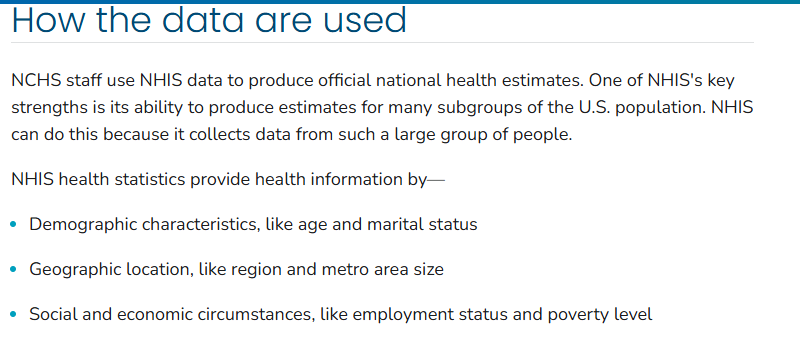
\includegraphics[width=0.9\linewidth,height=\textheight,keepaspectratio]{references/data-sources/../../assets/images/data1/nhis5.png}
\end{center}

\subsection*{About the Data}\label{about-the-data}
\addcontentsline{toc}{subsection}{About the Data}

If you click on \texttt{About\ the\ Data} link, you will find
information about the NHIS questionnaires, datasets, and documentation:

\begin{center}

\includegraphics[width=0.9\linewidth,height=\textheight,keepaspectratio]{references/data-sources/../../assets/images/data1/nhis6.png}
\end{center}

\marginnote{\begin{footnotesize}

\href{https://www.cdc.gov/nchs/nhis/documentation/index.html}{NHIS Data,
Questionnaires and Related Documentation}

\end{footnotesize}}

Under the \texttt{Overview} tab, you will find information about
different NHIS cycles and the questionnaires, datasets, and
documentation available in each cycle. As an example, let's click on the
\texttt{2023\ NHIS\ Questionnaires,\ Datasets,\ and\ Documentation} link
to see the details for the 2023 NHIS:

\begin{center}
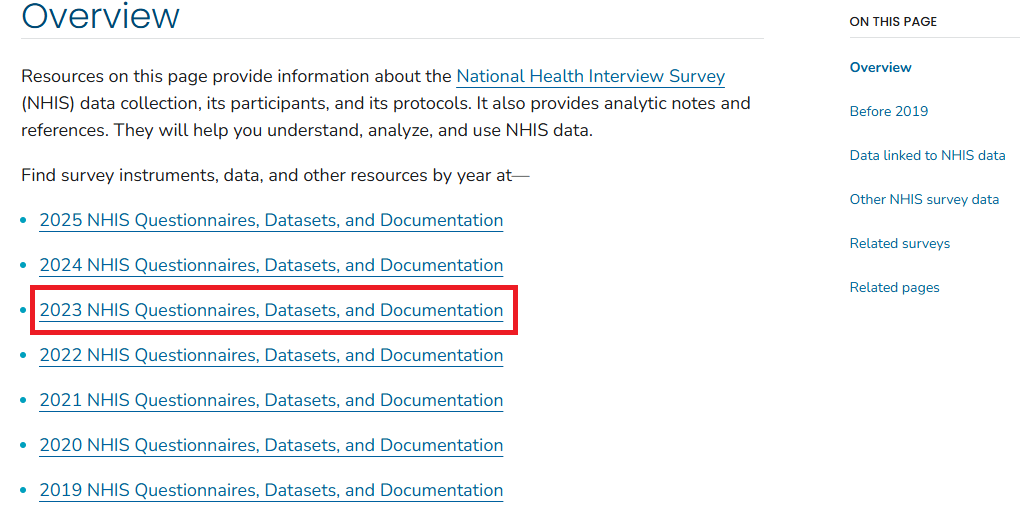
\includegraphics[width=0.9\linewidth,height=\textheight,keepaspectratio]{references/data-sources/../../assets/images/data1/nhis7.png}
\end{center}

\subsection*{NHIS Questionnaires, Datasets, and
Documentation}\label{nhis-questionnaires-datasets-and-documentation}
\addcontentsline{toc}{subsection}{NHIS Questionnaires, Datasets, and
Documentation}

To view the description of the 2023 NHIS, click on the
\texttt{Survey\ description\ document} link:

\begin{center}

\includegraphics[width=0.9\linewidth,height=\textheight,keepaspectratio]{references/data-sources/../../assets/images/data1/nhis8.png}
\end{center}

This will open the PDF of the 2023 NHIS survey description.
Alternatively, you can right-click on the link, click on
\texttt{Save\ link\ as...} and save the PDF file on your computer for
future reference.

\begin{center}
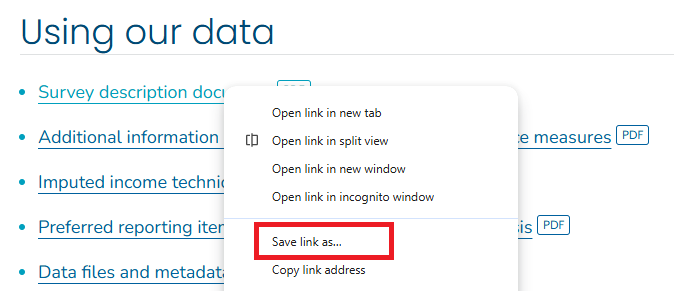
\includegraphics[width=0.9\linewidth,height=\textheight,keepaspectratio]{references/data-sources/../../assets/images/data1/nhis9.png}
\end{center}

Similarly, you can open and save the questionnaires and related
materials under the \texttt{Questionnaires\ and\ survey\ materials} tab.

\marginnote{\begin{footnotesize}

Data are available in 5 categories:

\begin{itemize}
\tightlist
\item
  Sample adult interview
\item
  Sample child interview
\item
  Parent-child pair data
\item
  Imputed income
\item
  Paradata
\end{itemize}

\end{footnotesize}}

In the recent NHIS, data are available in 5 categories: interview data
for adults, interview data for children, data for parent-child pairs,
imputed income, and paradata. You can click each link for documentation
to see a summary of the data and the codebook.

\begin{center}
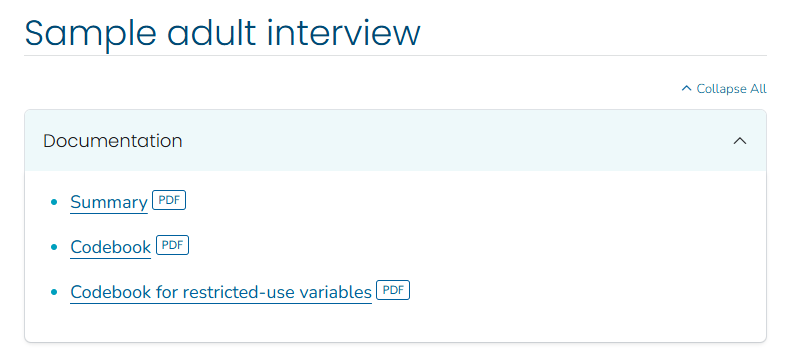
\includegraphics[width=0.9\linewidth,height=\textheight,keepaspectratio]{references/data-sources/../../assets/images/data1/nhis10.png}
\end{center}

\subsection*{NHIS Data}\label{nhis-data}
\addcontentsline{toc}{subsection}{NHIS Data}

The data files are stored on the NHIS website in different formats. You
can save the dataset in any statistical package that supports these file
formats, e.g., ASCII, CSV, SAS. Let us save the \texttt{adult} dataset
in the CSV format, which is in a zip file.

\begin{center}
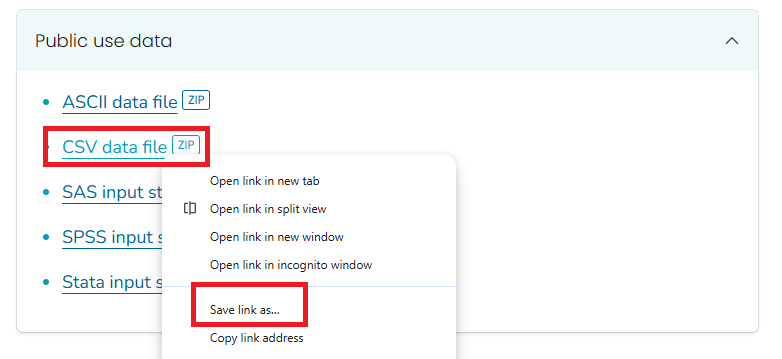
\includegraphics[width=0.9\linewidth,height=\textheight,keepaspectratio]{references/data-sources/../../assets/images/data1/nhis11.png}
\end{center}

\begin{center}
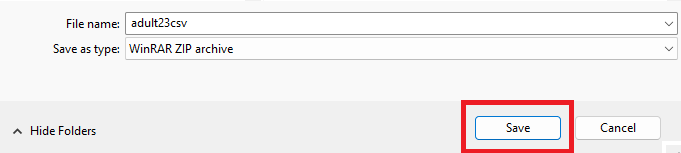
\includegraphics[width=0.9\linewidth,height=\textheight,keepaspectratio]{references/data-sources/../../assets/images/data1/nhis12.png}
\end{center}

The next step is to unzip the file to extract the CSV. Depending on your
computer, you can unzip the file with or without software. For example,
if you are using Windows, you can right-click the zip file and select
\texttt{Extract\ All...} to unzip it.

\begin{center}
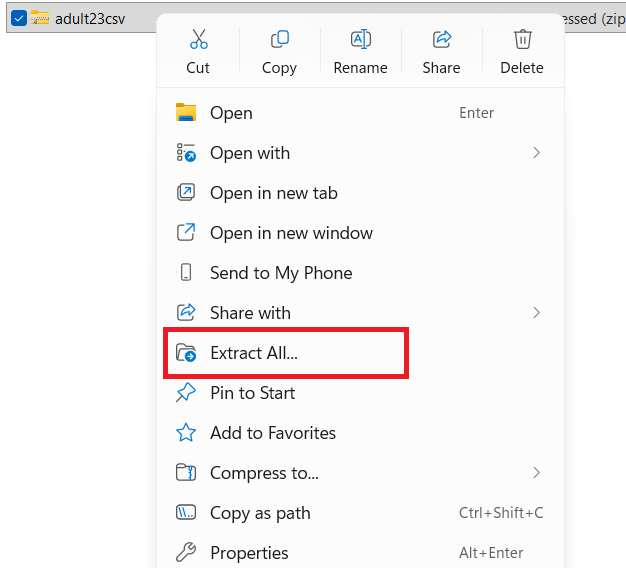
\includegraphics[width=0.9\linewidth,height=\textheight,keepaspectratio]{references/data-sources/../../assets/images/data1/nhis13.png}
\end{center}

Once unzipped, you will find two files: the CSV file for the dataset and
a readme file with some instructions. Below is the example for the
\texttt{adult} dataset:

\begin{center}
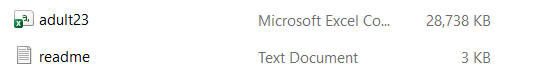
\includegraphics[width=0.9\linewidth,height=\textheight,keepaspectratio]{references/data-sources/../../assets/images/data1/nhis14.png}
\end{center}

To open the datafile in Excel, - you can double click on the CSV file,
or - right click on the CSV file and click on \texttt{Open}.

Later, you will learn how to open the data file in different statistical
software. For Excel, it would take a few seconds/minutes because of the
large size of the dataset. Once you open the data file, you will see the
data in a tabular format with rows and columns.

\begin{center}
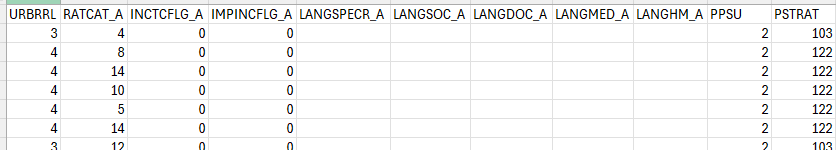
\includegraphics[width=0.9\linewidth,height=\textheight,keepaspectratio]{references/data-sources/../../assets/images/data1/nhis15.png}
\end{center}

\begin{itemize}
\tightlist
\item
  Each row represents a person.
\item
  Each column represents a variable.
\item
  The first row contains the variable names. The remaining rows contain
  the data for each person.
\end{itemize}

\subsection*{Use of the codebook}\label{use-of-the-codebook}
\addcontentsline{toc}{subsection}{Use of the codebook}

To understand the variables in the dataset, you can refer to the
codebook. The codebook provides information about the variable names,
labels, and values. For example, we want to understand the variable
\texttt{SEX\_A}:

\begin{center}
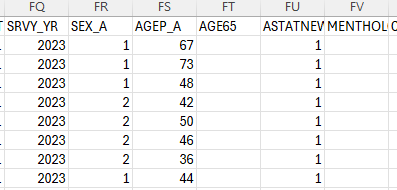
\includegraphics[width=0.9\linewidth,height=\textheight,keepaspectratio]{references/data-sources/../../assets/images/data1/nhis16.png}
\end{center}

We can look for \texttt{SEX\_A} in the codebook, which will provide us
with the variable label and the values for that variable (e.g., 1 for
Male, 2 for Female, and so on).

\begin{center}
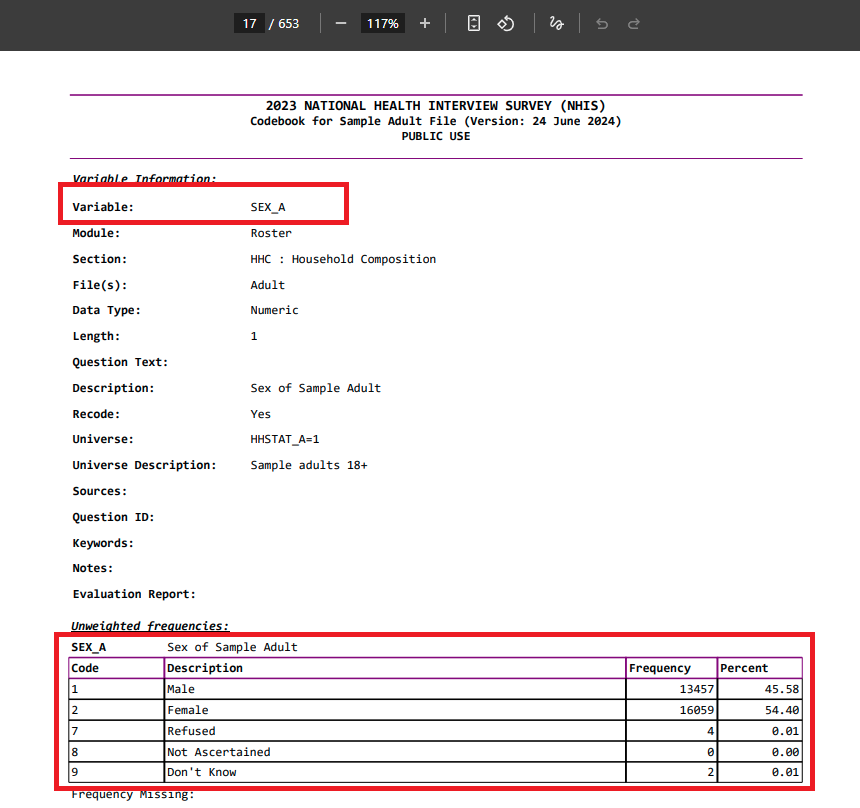
\includegraphics[width=0.9\linewidth,height=\textheight,keepaspectratio]{references/data-sources/../../assets/images/data1/nhis17.png}
\end{center}

There are so many variables in the dataset, and it is not possible to
understand all of them at once. You can refer to the codebook to
understand the variables that you are interested in for your analysis.
For example, the \texttt{WTFA\_A} variable is the sample adult weight
variable used to calculate weighted estimates for the US adult
population. Similarly, the \texttt{HYPEV\_A} variable is the
hypertension ever variable, indicating whether a doctor or other health
professional has ever told the person they have hypertension. Again, you
can refer to the codebook to understand the variables that you are
interested in.

\chapter*{NHANES}\label{nhanes}
\addcontentsline{toc}{chapter}{NHANES}

\markboth{NHANES}{NHANES}

The National Health and Nutrition Examination Survey (NHANES) is a
cross-sectional survey conducted by the US Centers for Disease Control
(CDC). The survey collects information on the health and nutritional
status of the US population. The survey includes interviews, physical
examinations, and laboratory tests.

\begin{center}

\includegraphics[width=0.9\linewidth,height=\textheight,keepaspectratio]{references/data-sources/../../assets/images/data2/nhanes1.png}
\end{center}

\marginnote{\begin{footnotesize}

\href{https://wwwn.cdc.gov/nchs/nhanes/Default.aspx}{CDC website for
NHANES}

\end{footnotesize}}

\subsection*{About NHANES}\label{about-nhanes}
\addcontentsline{toc}{subsection}{About NHANES}

You can find more information about the NHANES survey by clicking on
\href{https://www.cdc.gov/nchs/nhanes/about/}{About NHANES}:

\begin{center}

\includegraphics[width=0.9\linewidth,height=\textheight,keepaspectratio]{references/data-sources/../../assets/images/data2/nhanes2.png}
\end{center}

\begin{center}

\includegraphics[width=0.9\linewidth,height=\textheight,keepaspectratio]{references/data-sources/../../assets/images/data2/nhanes3.png}
\end{center}

On the \texttt{About\ NHANES} page, you will find information about what
the survey collects, data and documentation, the instructions on how to
use the data, and information on related NHANES surveys.

\begin{center}
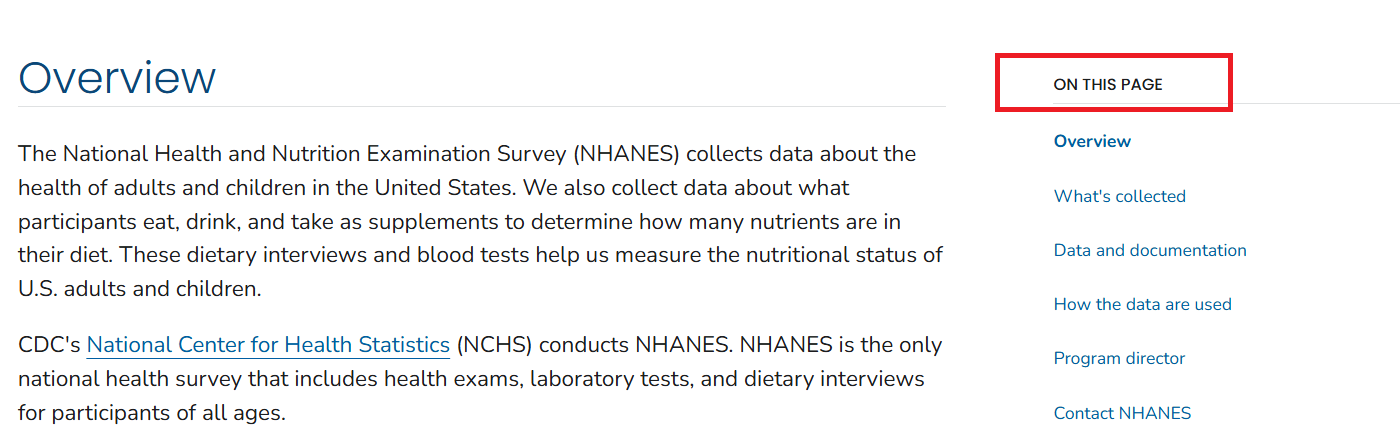
\includegraphics[width=0.9\linewidth,height=\textheight,keepaspectratio]{references/data-sources/../../assets/images/data2/nhanes4.png}
\end{center}

You can click on each of the links or scroll down to find information on
each of these topics one by one. For example, if we click on the
\texttt{Data\ and\ documentation} link, we will find information as
follows:

\begin{center}
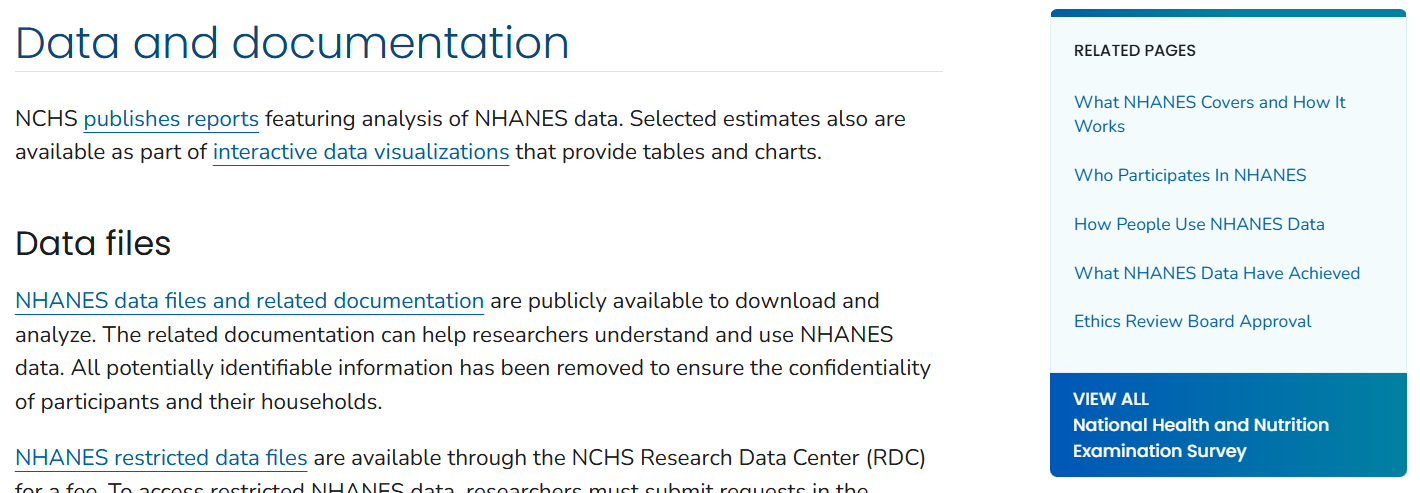
\includegraphics[width=0.9\linewidth,height=\textheight,keepaspectratio]{references/data-sources/../../assets/images/data2/nhanes5.png}
\end{center}

\subsection*{Survey Methods and Analytic
Guidelines}\label{survey-methods-and-analytic-guidelines}
\addcontentsline{toc}{subsection}{Survey Methods and Analytic
Guidelines}

If you click on
\texttt{NHANES\ data\ files\ and\ related\ documentation} link, you will
find information about the NHANES questionnaires, datasets, and
documentation:

\begin{center}
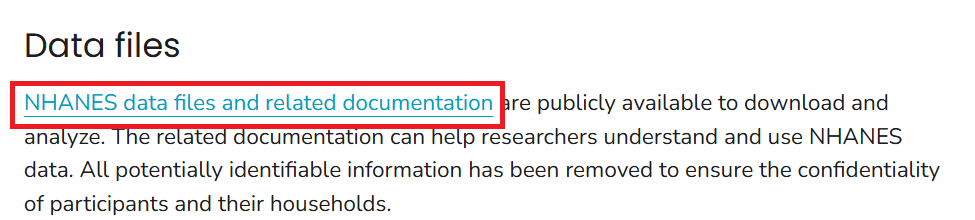
\includegraphics[width=0.9\linewidth,height=\textheight,keepaspectratio]{references/data-sources/../../assets/images/data2/nhanes6.png}
\end{center}

\begin{center}
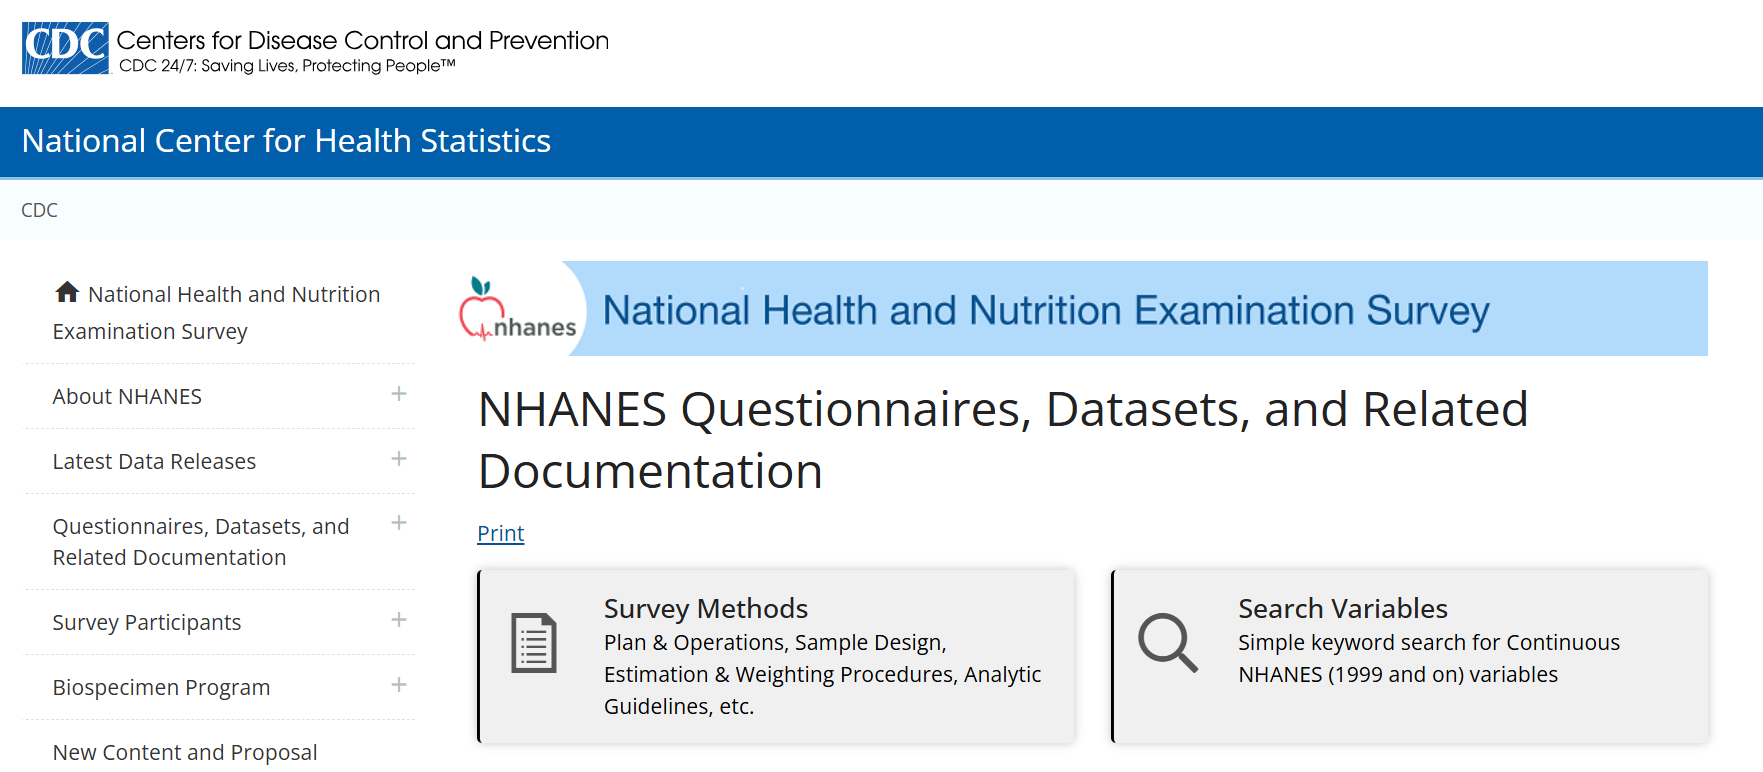
\includegraphics[width=0.9\linewidth,height=\textheight,keepaspectratio]{references/data-sources/../../assets/images/data2/nhanes7.png}
\end{center}

\marginnote{\begin{footnotesize}

\href{https://wwwn.cdc.gov/nchs/nhanes/Default.aspx}{NHANES data files
and related documentation}

\end{footnotesize}}

You can click \texttt{Survey\ Methods} to find information on survey
methods and analytic guidelines. The
\texttt{Survey\ Methods\ and\ Analytic\ Guidelines} page provides
information about the plan and operation of the NHANES survey, the
sampling design, methods for calculating weights and variance
estimation, and guidelines for analyzing NHANES data, along with links
to related resources.

\begin{center}
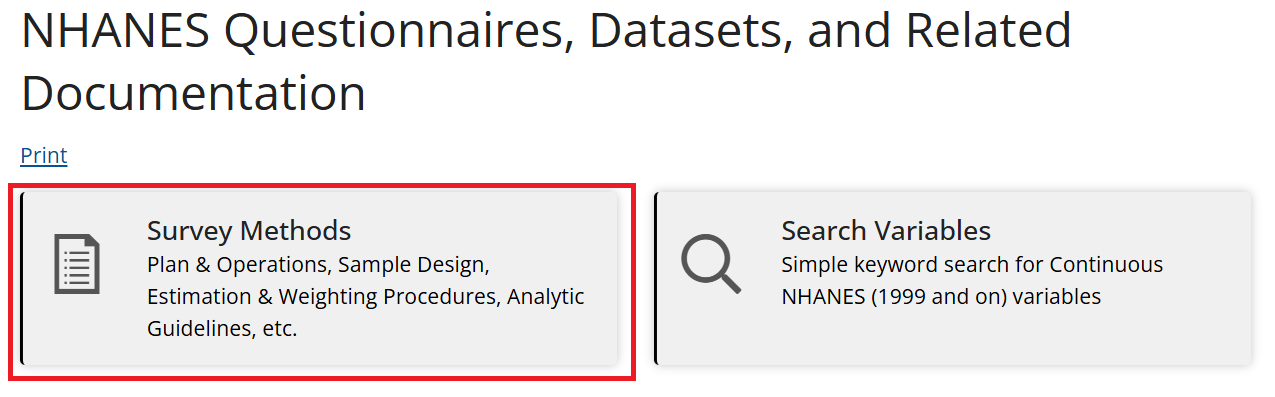
\includegraphics[width=0.9\linewidth,height=\textheight,keepaspectratio]{references/data-sources/../../assets/images/data2/nhanes8.png}
\end{center}

\subsection*{Search Variables}\label{search-variables}
\addcontentsline{toc}{subsection}{Search Variables}

If you click on \texttt{Search\ Variables} link, you will find a search
tool to search for variables in the NHANES datasets (1999 and on).

\begin{center}
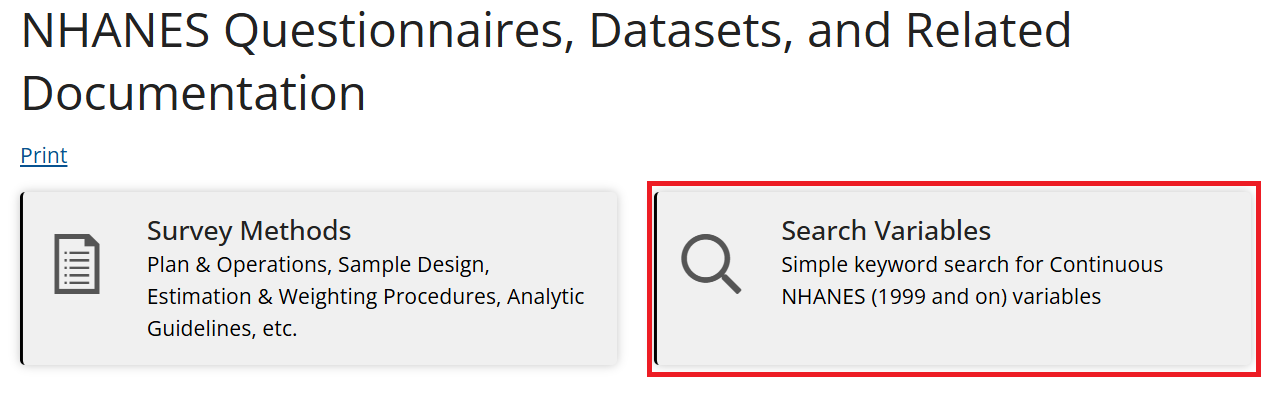
\includegraphics[width=0.9\linewidth,height=\textheight,keepaspectratio]{references/data-sources/../../assets/images/data2/nhanes9.png}
\end{center}

You can search for variables by entering keywords in the search box. For
example, if you enter \texttt{diabetes} in the search box, you will find
a list of variables related to diabetes in the NHANES datasets.

\begin{center}
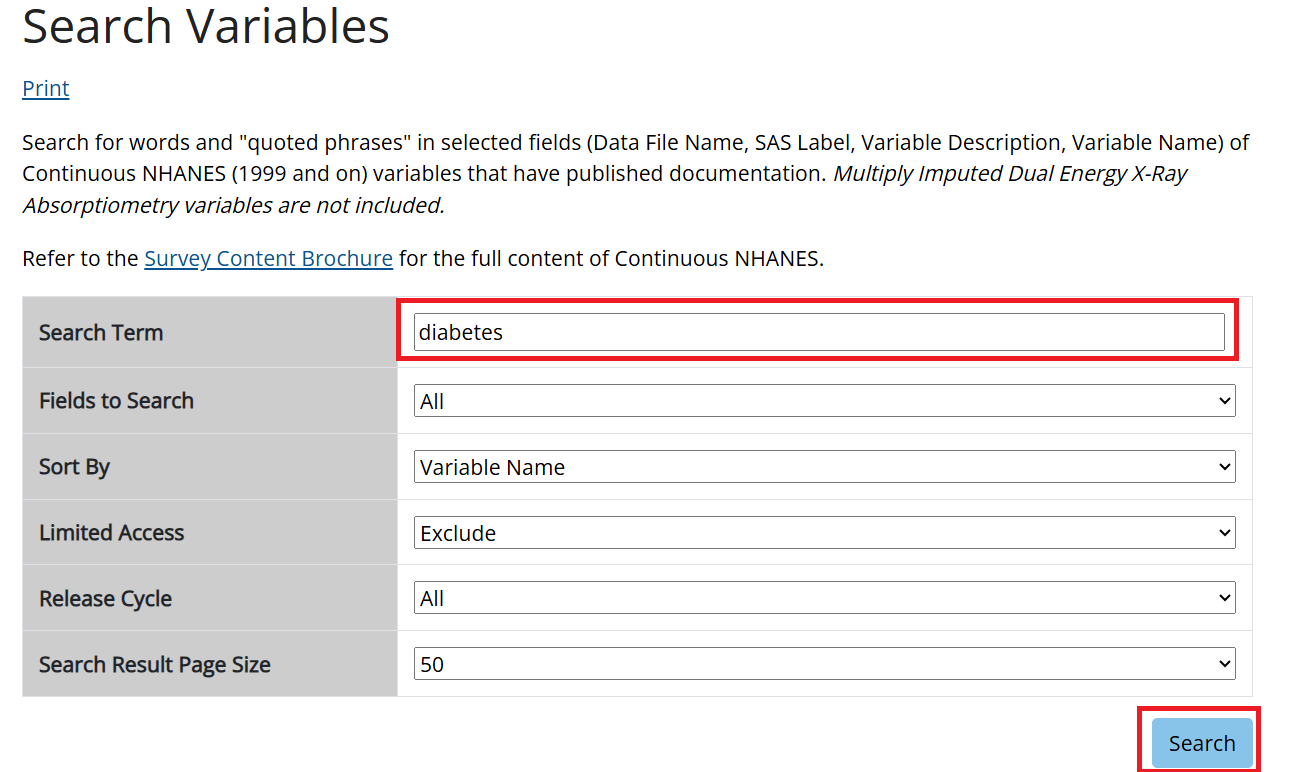
\includegraphics[width=0.9\linewidth,height=\textheight,keepaspectratio]{references/data-sources/../../assets/images/data2/nhanes10.png}
\end{center}

\begin{center}
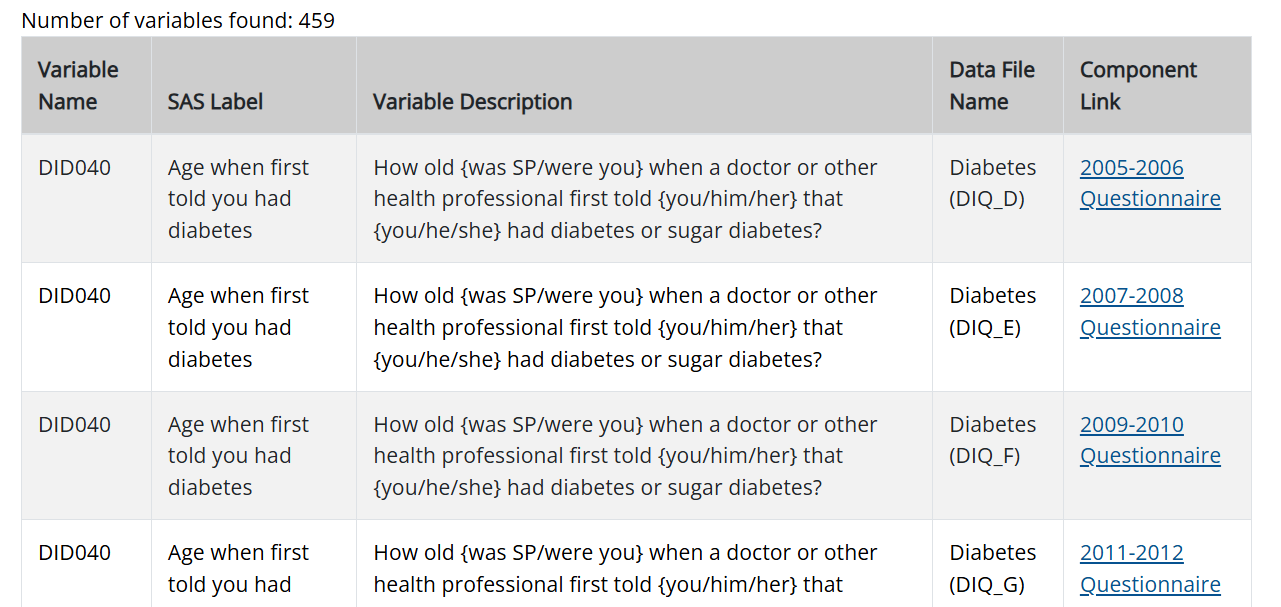
\includegraphics[width=0.9\linewidth,height=\textheight,keepaspectratio]{references/data-sources/../../assets/images/data2/nhanes11.png}
\end{center}

You can restrict your search to a specific NHANES cycle by selecting the
cycle from the drop-down menu. For example, if you select the
\texttt{2017-2018} cycle, you will find a list of variables related to
diabetes in the 2017-2018 NHANES dataset.

\begin{center}
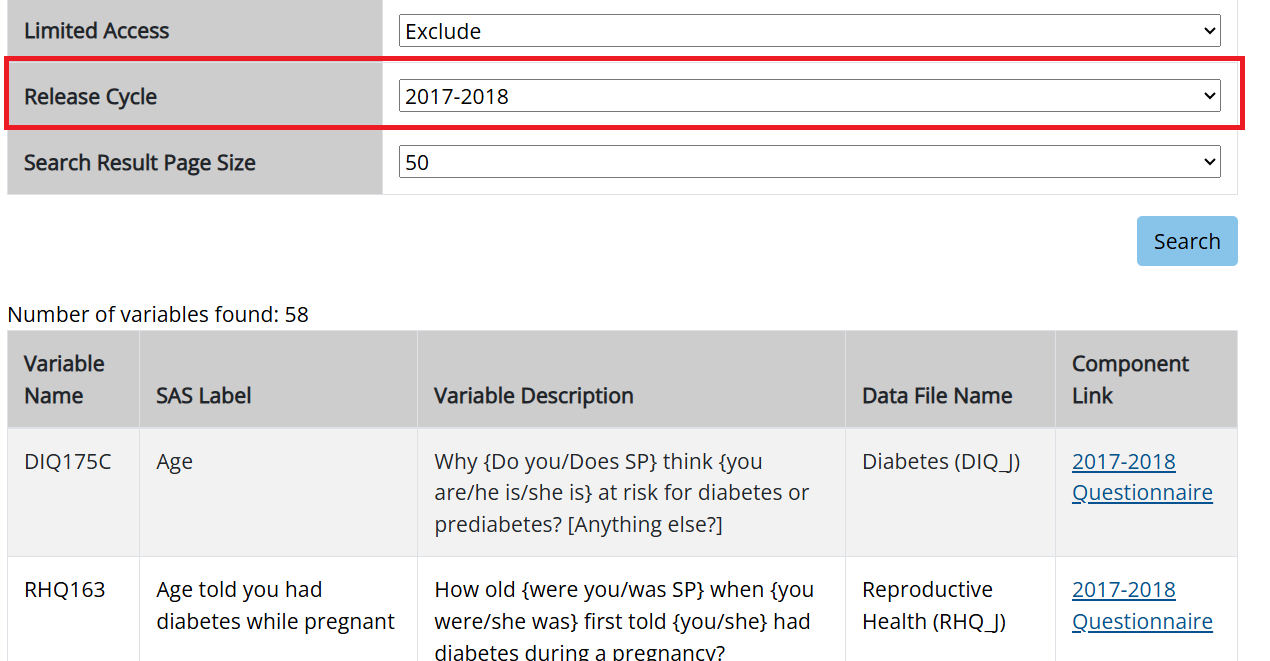
\includegraphics[width=0.9\linewidth,height=\textheight,keepaspectratio]{references/data-sources/../../assets/images/data2/nhanes12.png}
\end{center}

\subsection*{NHANES Questionnaires, Datasets, and
Documentation}\label{nhanes-questionnaires-datasets-and-documentation}
\addcontentsline{toc}{subsection}{NHANES Questionnaires, Datasets, and
Documentation}

Let's explore the questionnaires, datasets, and documentation for the
2017-2018 NHANES cycle. You need to click on \texttt{NHANES\ 2017-2018}
under the \texttt{Continuous\ NHANES} tab:

\begin{center}
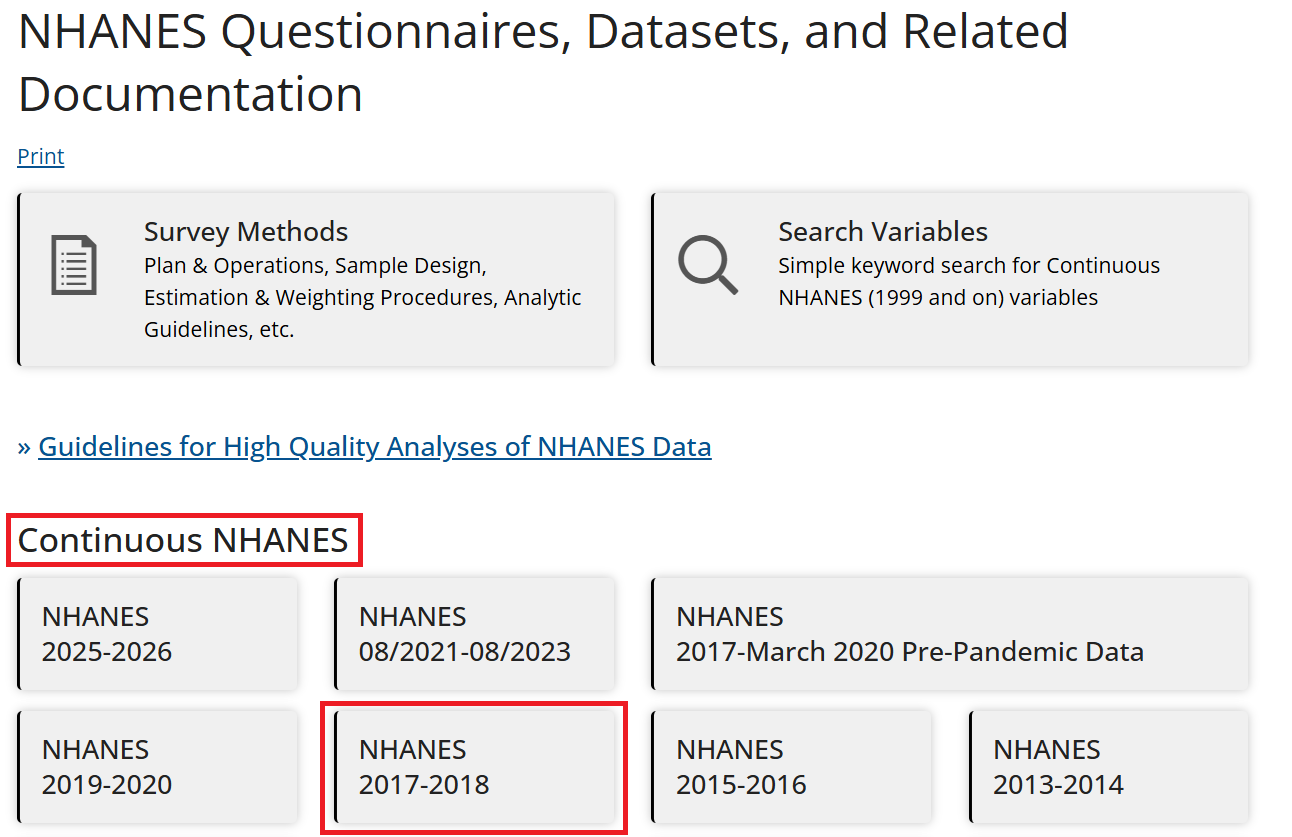
\includegraphics[width=0.9\linewidth,height=\textheight,keepaspectratio]{references/data-sources/../../assets/images/data2/nhanes13.png}
\end{center}

This will open the page for the 2017-2018 NHANES cycle, where you can
find information on the survey description, questionnaires, datasets,
and documentation.

\begin{center}
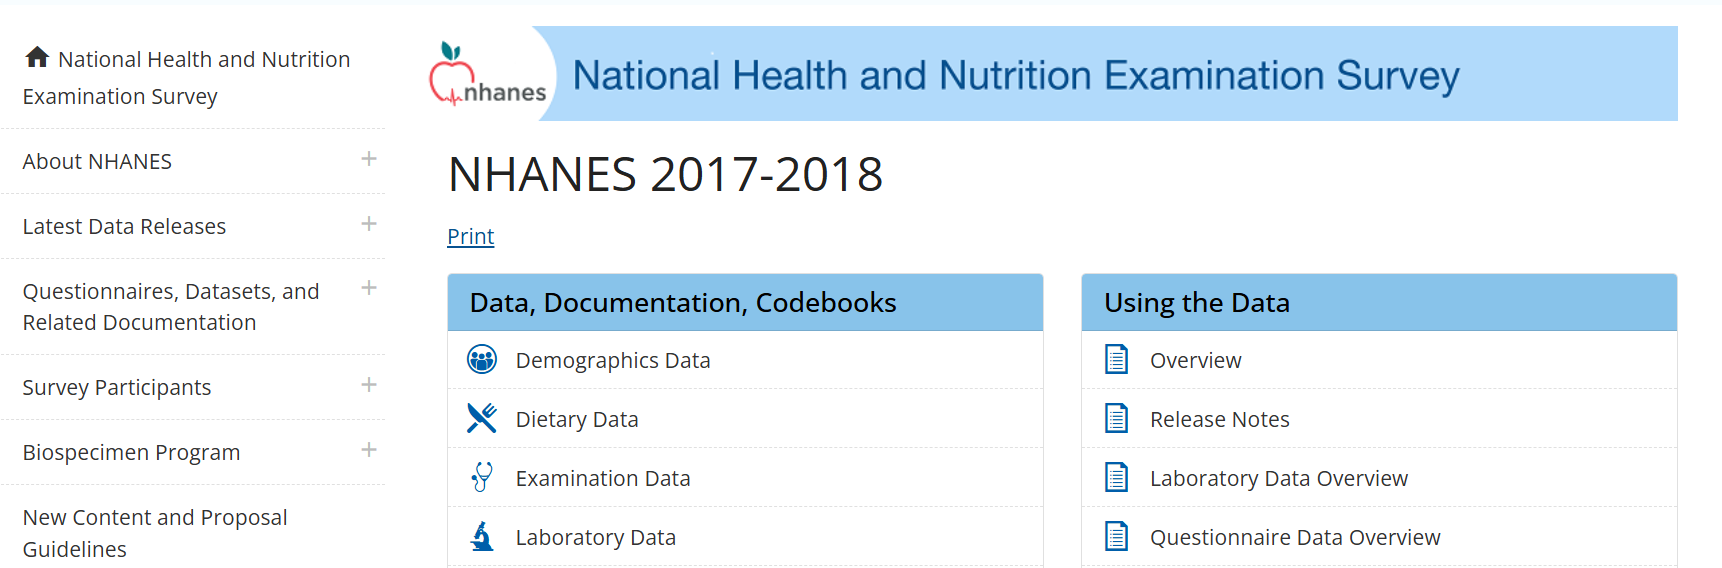
\includegraphics[width=0.9\linewidth,height=\textheight,keepaspectratio]{references/data-sources/../../assets/images/data2/nhanes14.png}
\end{center}

\marginnote{\begin{footnotesize}

Data are available in 6 categories:

\begin{itemize}
\tightlist
\item
  Demographics
\item
  Dietary
\item
  Examination
\item
  Laboratory
\item
  Questionnaire
\item
  Limited Access
\end{itemize}

\end{footnotesize}}

There are six categories of data available for the 2017-2018 NHANES
cycle: Demographics, Dietary, Examination, Laboratory, Questionnaire,
and Limited Access data. You can click each category to find the
datasets and documentation available in that category. For example, if
you click on \texttt{Demographics\ Data}, you will find a list of
datasets and documentation related to demographics data in the 2017-2018
NHANES cycle.

\begin{center}
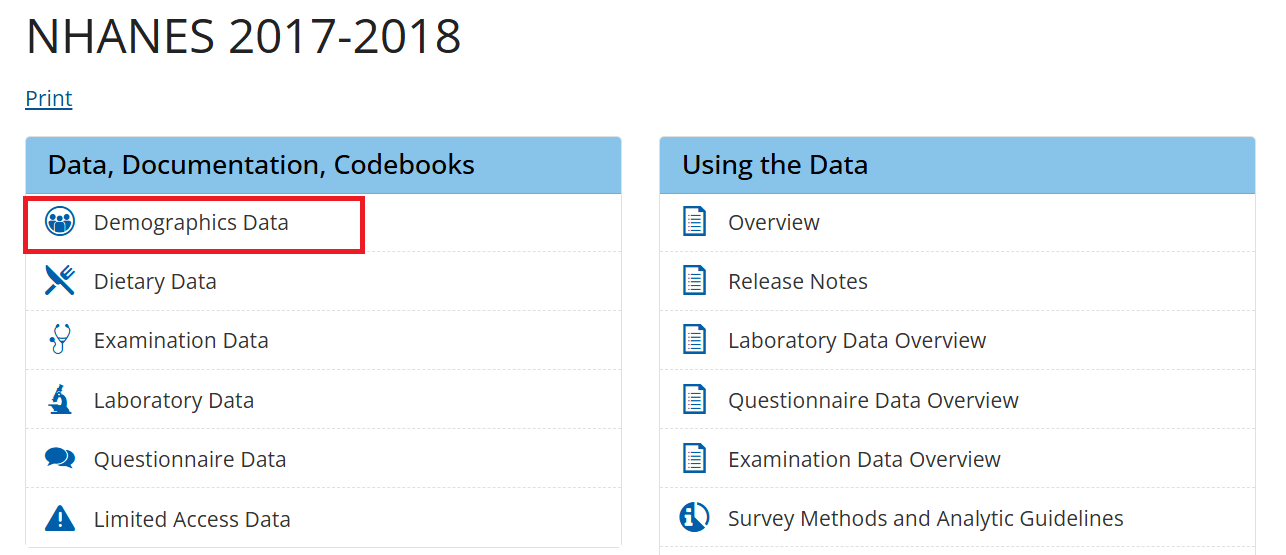
\includegraphics[width=0.9\linewidth,height=\textheight,keepaspectratio]{references/data-sources/../../assets/images/data2/nhanes15.png}
\end{center}

\begin{center}
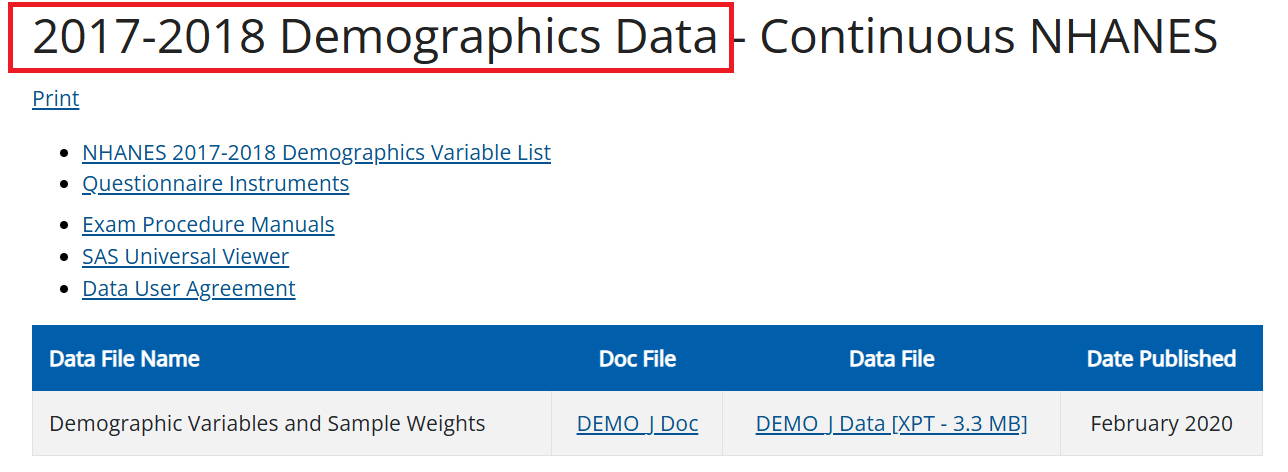
\includegraphics[width=0.9\linewidth,height=\textheight,keepaspectratio]{references/data-sources/../../assets/images/data2/nhanes16.png}
\end{center}

There is a \texttt{Doc\ File} available for each dataset that provides
information about the dataset, including the variables it contains,
their coding, and any special considerations for using it. It is
important to read the \texttt{Doc} file before using the dataset to
understand the data structure and how to use it properly. The
\texttt{Data\ File} contains the dataset data in \texttt{.XPT} format,
which is a SAS Transport file, not a CSV.

\begin{center}
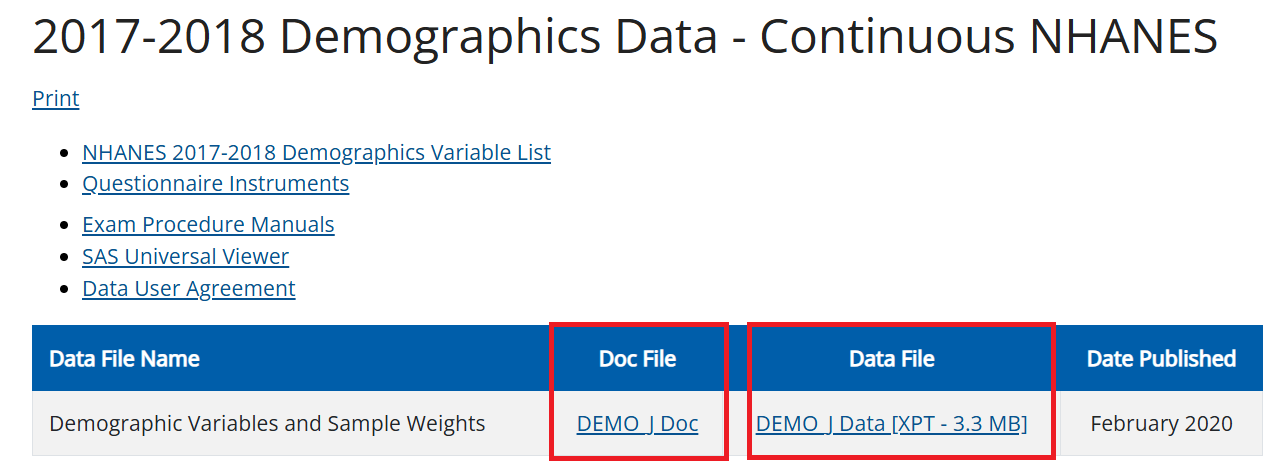
\includegraphics[width=0.9\linewidth,height=\textheight,keepaspectratio]{references/data-sources/../../assets/images/data2/nhanes17.png}
\end{center}

\subsection*{Data}\label{data}
\addcontentsline{toc}{subsection}{Data}

You need to click on the \texttt{DEMO\_J\ Data\ {[}XPT\ -\ 3.3\ MB{]}}
link to download the dataset. Note that you cannot easily open an
\texttt{.XPT} file in Excel or Google Sheets. In the real world, data
isn't always in a friendly format. For this week, let's download the
\texttt{NHANES\_Demo\_Converted.csv} file from our Canvas page to look
at the rows. Later, we will use an AI co-pilot to write R code that
reads \texttt{.XPT} files automatically.

Let's open the \texttt{NHANES\_Demo\_Converted.csv} file in Excel and
see the first few rows:

\begin{center}
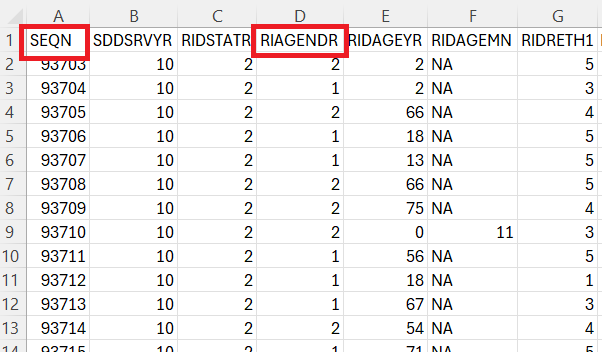
\includegraphics[width=0.9\linewidth,height=\textheight,keepaspectratio]{references/data-sources/../../assets/images/data2/nhanes18.png}
\end{center}

\begin{itemize}
\tightlist
\item
  Each row represents a person.
\item
  Each column represents a variable.
\item
  The first row contains the variable names. The remaining rows contain
  the data for each person.
\end{itemize}

For example, \texttt{SEQN} is the unique identifier for each person in
the dataset, and \texttt{RIAGENDR} is the variable for gender.

\subsection*{Use of the Codebook}\label{use-of-the-codebook-1}
\addcontentsline{toc}{subsection}{Use of the Codebook}

To understand the variables in the dataset, you can refer to the
codebook. The codebook provides information about the variable names,
labels, and values. The \texttt{Doc\ File} explained earlier contains
the codebook for the dataset. You need to click on the
\texttt{DEMO\_J\ Doc} link to open the codebook on a new page. Let's we
want to understand the variables \texttt{SEQN} and \texttt{RIAGENDR}:

\begin{center}
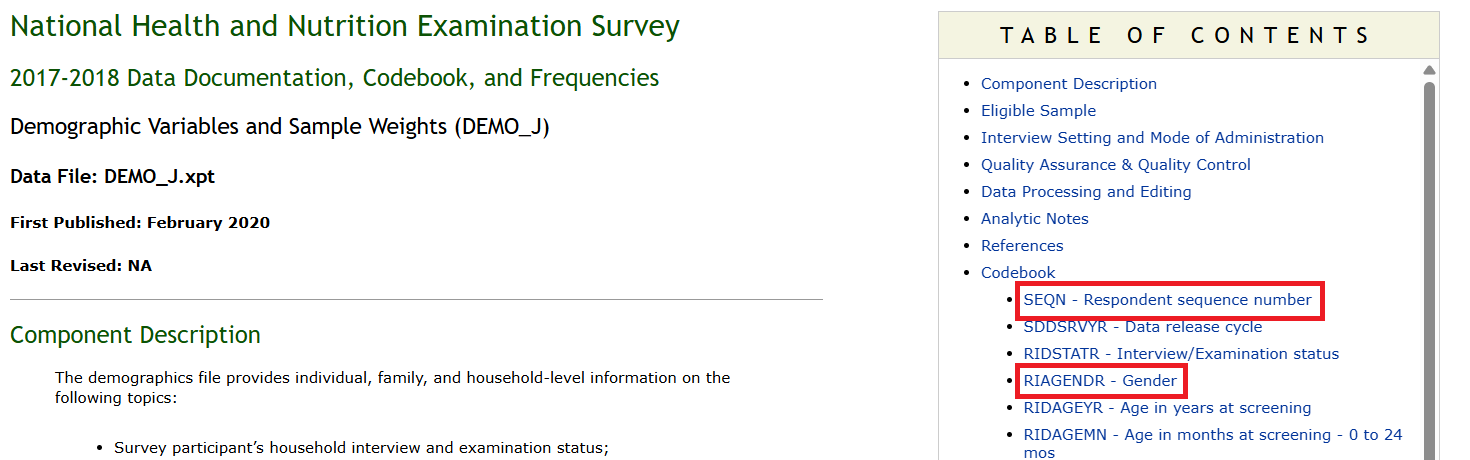
\includegraphics[width=0.9\linewidth,height=\textheight,keepaspectratio]{references/data-sources/../../assets/images/data2/nhanes19.png}
\end{center}

You need to click on the \texttt{SEQN\ -\ Respondent\ sequence\ number}
link or scroll down to find the information about the \texttt{SEQN}
variable.

\begin{center}
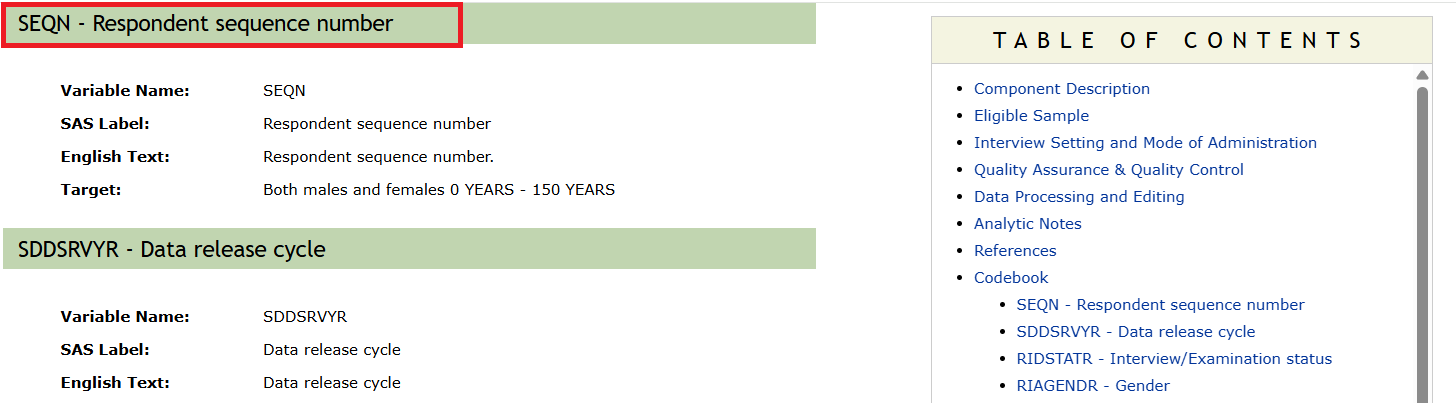
\includegraphics[width=0.9\linewidth,height=\textheight,keepaspectratio]{references/data-sources/../../assets/images/data2/nhanes20.png}
\end{center}

Similarly, you can click on the \texttt{RIAGENDR\ -\ Gender} link or
scroll down to find the information about the \texttt{RIAGENDR}
variable.

\begin{center}
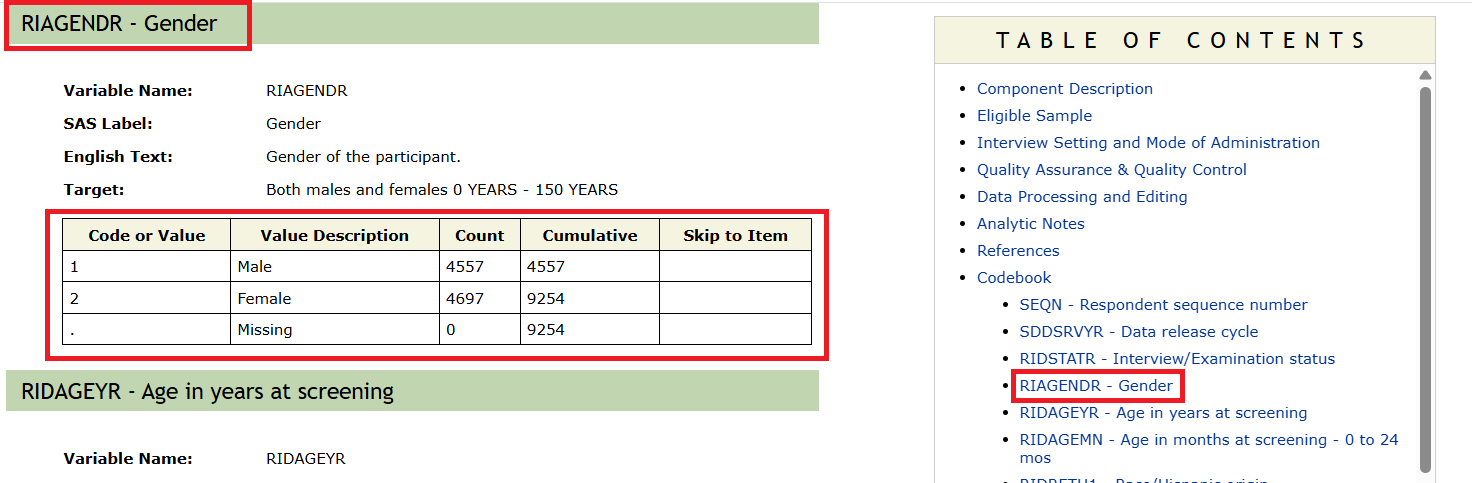
\includegraphics[width=0.9\linewidth,height=\textheight,keepaspectratio]{references/data-sources/../../assets/images/data2/nhanes21.png}
\end{center}

As you can see, the \texttt{RIAGENDR} variable has two values: 1 for
Male and 2 for Female, without any missing values. You can also see the
frequency of each value in the dataset. These numbers/frequencies should
exactly match the frequencies in your dataset. You can use the codebook
to understand other variables in the dataset. Similarly, you can use the
other data files (e.g., Dietary) and their codebook to understand the
variables in those datasets. Unlike the demographic file, which uses
only one dataset and one codebook, the other files use multiple datasets
and codebooks. As an example, if you click on the
\texttt{Questionnaire\ Data} link, you will find multiple datasets and
codebooks for questionnaire data:

\begin{center}
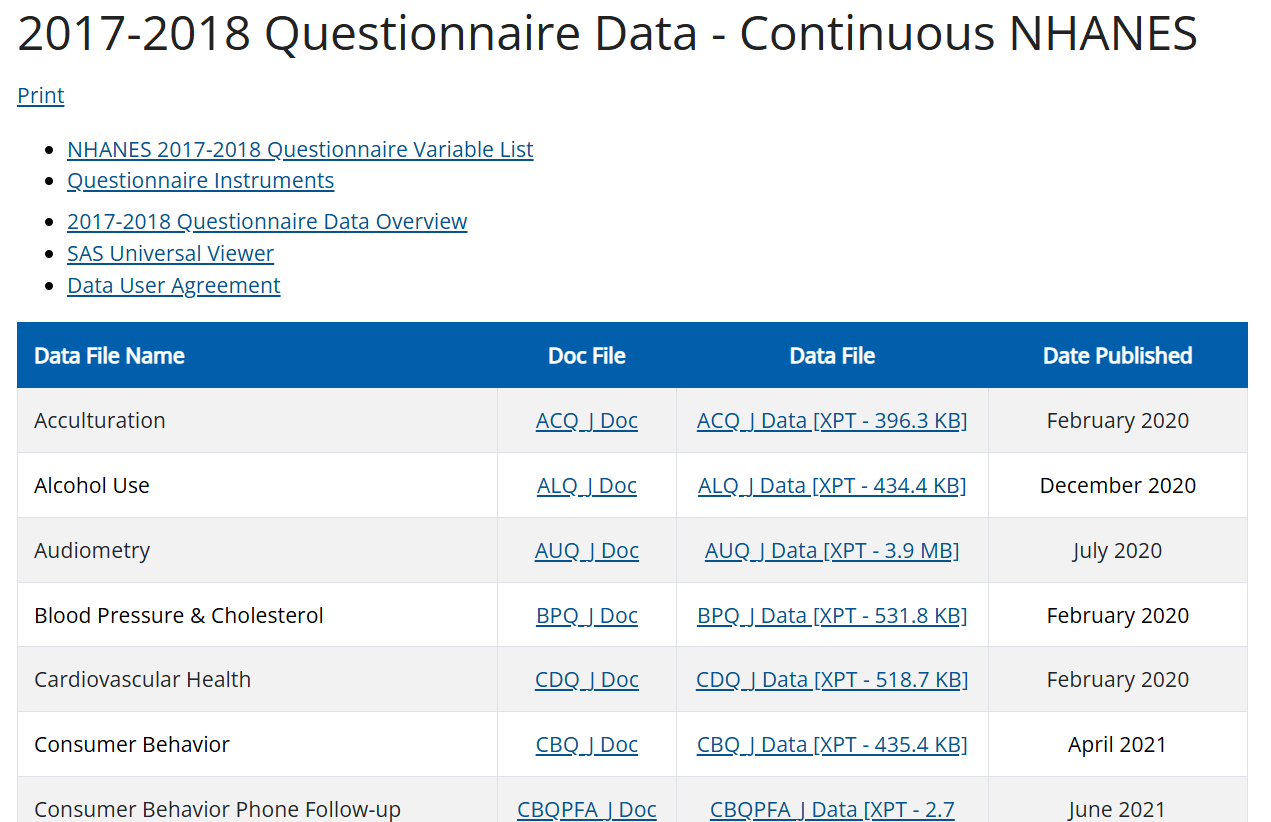
\includegraphics[width=0.9\linewidth,height=\textheight,keepaspectratio]{references/data-sources/../../assets/images/data2/nhanes22.png}
\end{center}

\chapter*{BRFSS}\label{brfss}
\addcontentsline{toc}{chapter}{BRFSS}

\markboth{BRFSS}{BRFSS}

The Behavioral Risk Factor Surveillance System (BRFSS) is a
cross-sectional survey conducted by the US Centers for Disease Control
(CDC). The survey collects information on health-related risk behaviors,
chronic health conditions, and use of preventive services among US
adults. BRFSS completes more than 400,000 adult interviews each year,
making it the largest continuously conducted health survey system in the
world.

\begin{center}
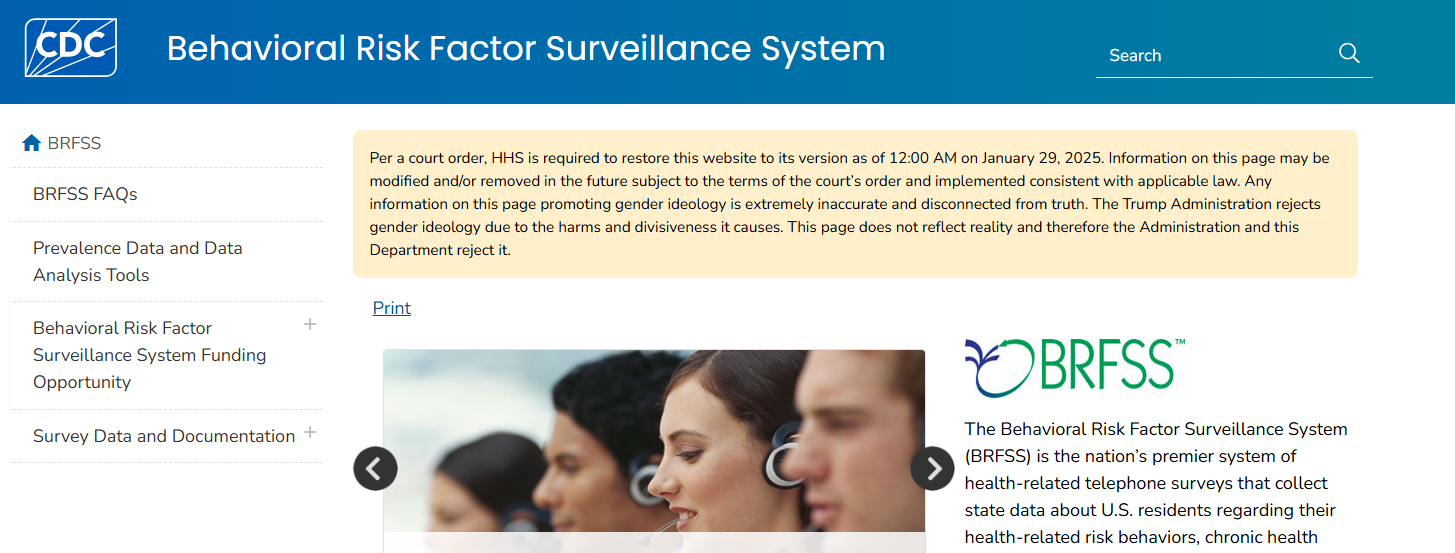
\includegraphics[width=0.9\linewidth,height=\textheight,keepaspectratio]{references/data-sources/../../assets/images/data3/BRFSS1.png}
\end{center}

\marginnote{\begin{footnotesize}

\href{https://www.cdc.gov/brfss/index.html}{CDC website for BRFSS}

\end{footnotesize}}

\subsection*{About BRFSS}\label{about-brfss}
\addcontentsline{toc}{subsection}{About BRFSS}

You can find more information about the BRFSS survey by clicking on
\href{https://www.cdc.gov/brfss/about/brfss_faq.htm}{BRFSS FAQs}:

\begin{center}
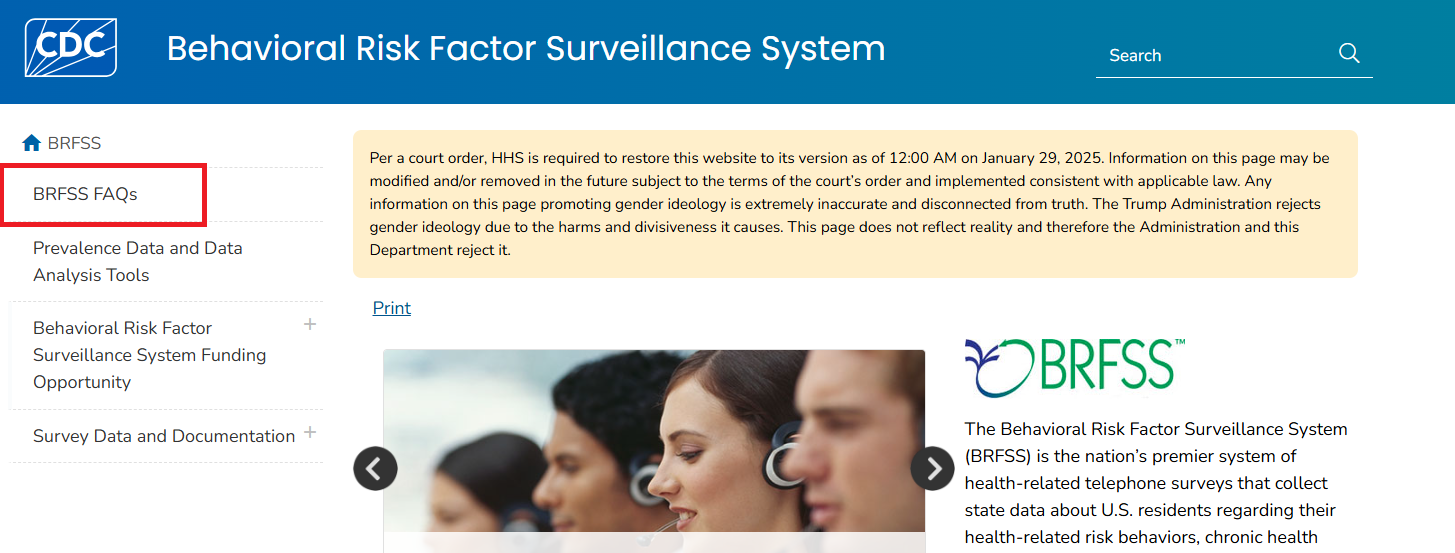
\includegraphics[width=0.9\linewidth,height=\textheight,keepaspectratio]{references/data-sources/../../assets/images/data3/BRFSS2.png}
\end{center}

On the \texttt{BRFSS\ FAQs} page, you will find information about the
BRFSS survey, including what the survey collects, how the survey is
conducted, and how to use the data.

\subsection*{Survey Data \&
Documentation}\label{survey-data-documentation}
\addcontentsline{toc}{subsection}{Survey Data \& Documentation}

If you click on \texttt{Survey\ Data\ \&\ Documentation} link, you will
find information about the BRFSS questionnaires, datasets, and
documentation:

\begin{center}
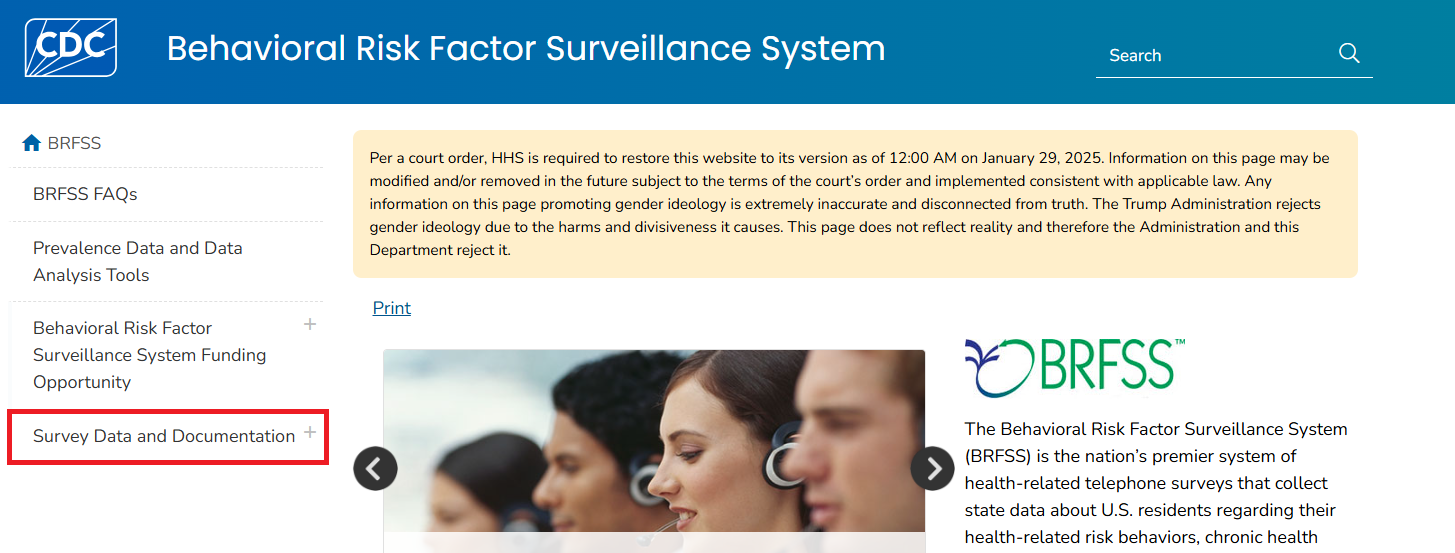
\includegraphics[width=0.9\linewidth,height=\textheight,keepaspectratio]{references/data-sources/../../assets/images/data3/BRFSS3.png}
\end{center}

\marginnote{\begin{footnotesize}

\href{https://www.cdc.gov/brfss/data_documentation/index.htm}{BRFSS
Survey Data \& Documentation}

\end{footnotesize}}

There are four types of data files available for download: 1) annual
data, 2) asthma call-back data, 3) GIS map data, and 4) SMART data. The
annual data files include information on health-related risk behaviors,
chronic health conditions, and use of preventive services among US
adults. The asthma call-back data files include information on
asthma-related health outcomes and healthcare utilization among adults
with asthma. The GIS map data files include information on the
geographic distribution of the data. The SMART (Selected
Metropolitan/Micropolitan Area Risk Trends) data provide prevalence
rates for selected conditions and behaviors for cities and their
surrounding counties.

\begin{center}
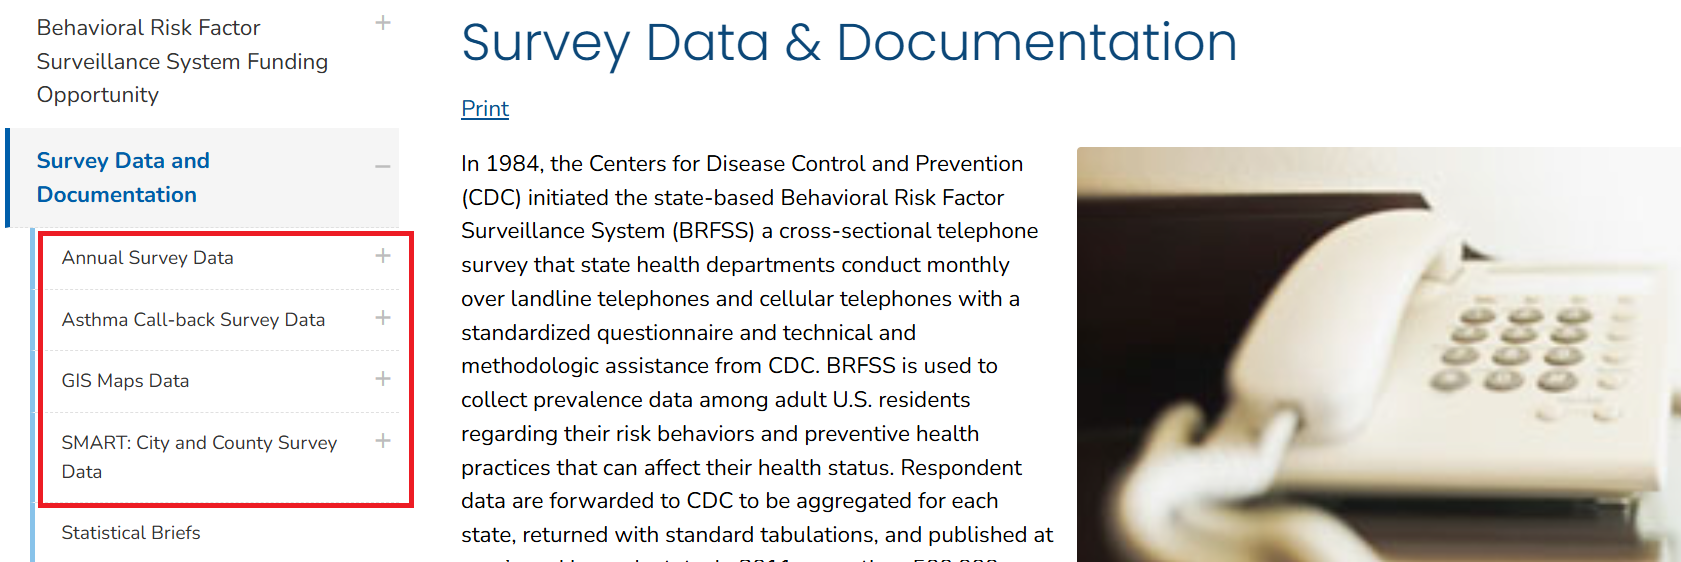
\includegraphics[width=0.9\linewidth,height=\textheight,keepaspectratio]{references/data-sources/../../assets/images/data3/BRFSS4.png}
\end{center}

For the annual data, you can click on the \texttt{Annual\ Survey\ Data}
link to find information about the annual data files, including how to
access the data, how to use the data, and how to analyze the data. There
are two types of annual data files available for download: 1) the raw
data files and 2) the prevalence and trends database.

\begin{center}
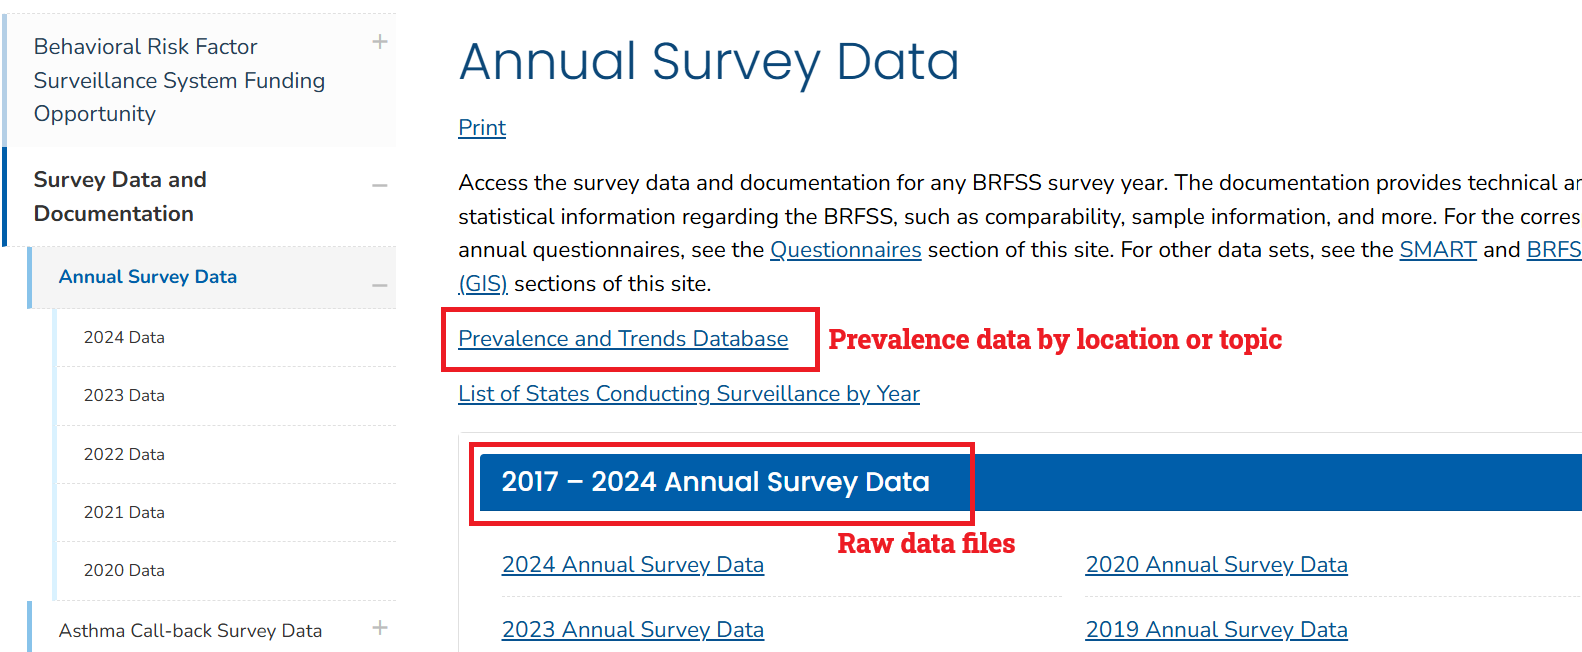
\includegraphics[width=0.9\linewidth,height=\textheight,keepaspectratio]{references/data-sources/../../assets/images/data3/BRFSS5.png}
\end{center}

\subsection*{Annual Survey Data}\label{annual-survey-data}
\addcontentsline{toc}{subsection}{Annual Survey Data}

There are separate links for each year of data, and you can click on
each link to find information about the data for that year. For example,
if you click on the \texttt{2023\ Annual\ Survey\ Data} link, you will
find information about the 2023 annual data files, including how to
access the data, how to use the data, and how to analyze the data.

\marginnote{\begin{footnotesize}

\href{https://www.cdc.gov/brfss/annual_data/annual_data.htm}{Annual
Survey Data}

\end{footnotesize}}

\begin{center}
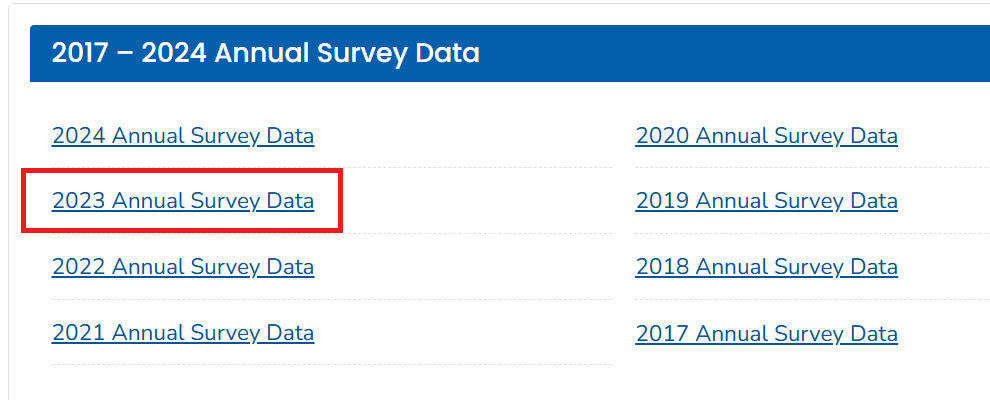
\includegraphics[width=0.9\linewidth,height=\textheight,keepaspectratio]{references/data-sources/../../assets/images/data3/BRFSS6.png}
\end{center}

\begin{center}
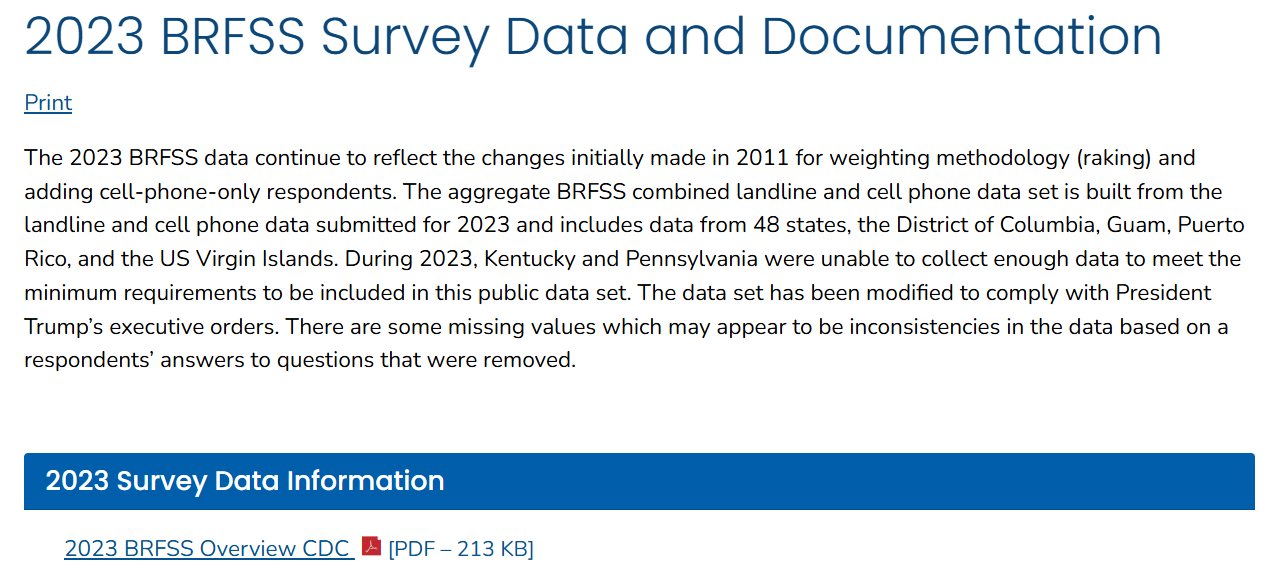
\includegraphics[width=0.9\linewidth,height=\textheight,keepaspectratio]{references/data-sources/../../assets/images/data3/BRFSS7.png}
\end{center}

The \texttt{2023\ BRFSS\ Survey\ Data\ and\ Documentation} page provides
information about three resources: 1) data information such as the
codebook and sampling weights, 2) data files in ASCII and SAS XPT
transport formats, and 3) SAS resources. To download/save the data
files, click the specific format you want. For example, if you click on
the \texttt{2023\ BRFSS\ Data\ (SAS\ Transport\ Format)} link, the
annual survey data for 2023 will be downloaded in a ZIP file that
contains the dataset in a \texttt{.XPT} format.

\begin{center}
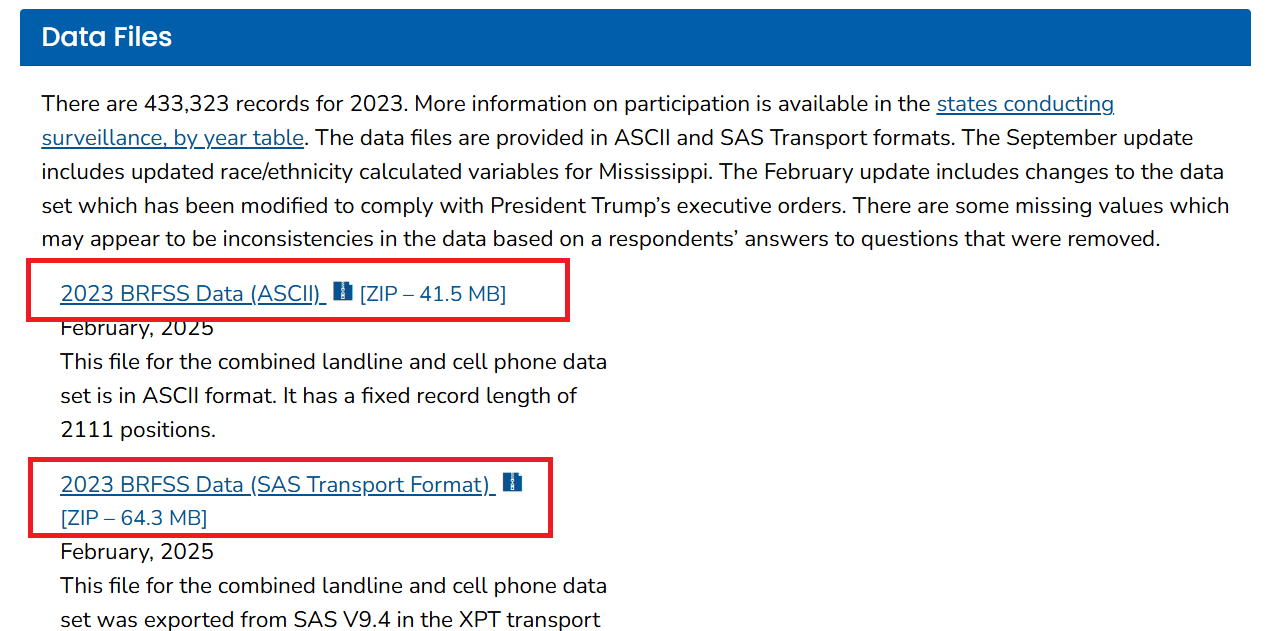
\includegraphics[width=0.9\linewidth,height=\textheight,keepaspectratio]{references/data-sources/../../assets/images/data3/BRFSS8.png}
\end{center}

You need to unzip the file to extract the data file in \texttt{.XPT}
format. However, opening the data file in Excel or Google Sheets is a
bit tricky. The SAS XPT (or ASCII) data file needs to be
converted/formatted appropriately before it can be opened in Excel or
Google Sheets. Many statistical software packages, such as R, SAS, or
STATA, can read the data file in \texttt{.XPT} format. Below is the data
file, where the column names are the variable names, and the rows are
the observations (i.e., survey respondents):

\begin{center}
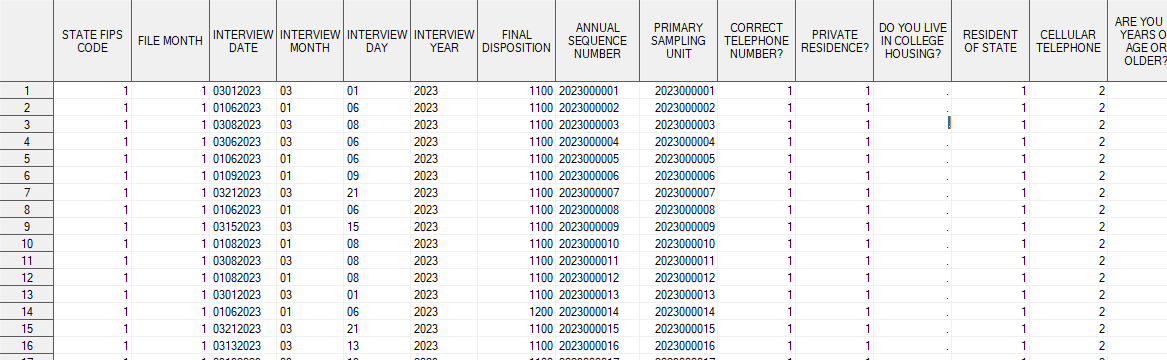
\includegraphics[width=0.9\linewidth,height=\textheight,keepaspectratio]{references/data-sources/../../assets/images/data3/BRFSS9.png}
\end{center}

To understand the variables in the dataset, you can refer to the
codebook:

\begin{center}
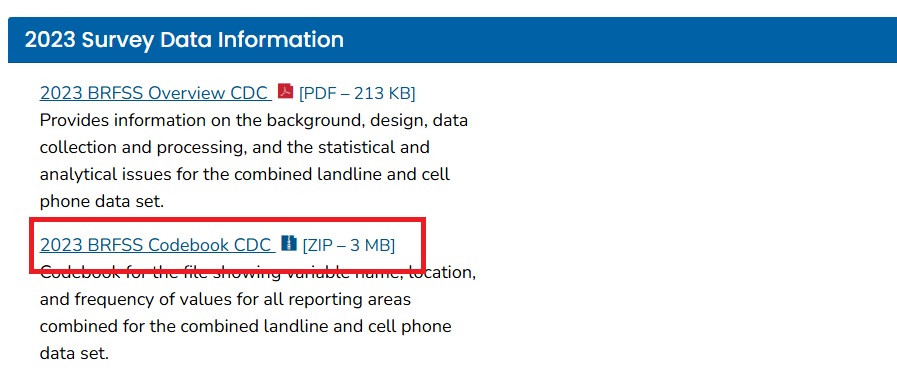
\includegraphics[width=0.9\linewidth,height=\textheight,keepaspectratio]{references/data-sources/../../assets/images/data3/BRFSS10.png}
\end{center}

You need to unzip the file to extract the codebook in HTML format. The
codebook provides information about the variable names, labels, and
values. For example, if you want to understand the variable
\texttt{Drinking\ and\ Driving}, you can find the variable name, label,
and values in the codebook:

\begin{center}
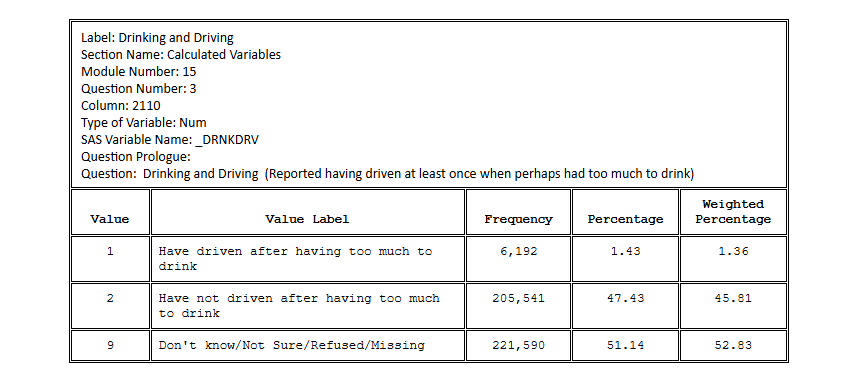
\includegraphics[width=0.9\linewidth,height=\textheight,keepaspectratio]{references/data-sources/../../assets/images/data3/BRFSS11.png}
\end{center}

You can similarly download the asthma call-back, GIS map, and SMART
datasets. To understand the variables in those datasets, you can refer
to the codebook for each dataset.

\marginnote{\begin{footnotesize}

\href{https://www.cdc.gov/brfss/acbs/index.htm}{Asthma Call-back Data}

\href{https://www.cdc.gov/brfss/gis/gis_maps.htm}{GIS Data}

\href{https://www.cdc.gov/brfss/smart/Smart_data.htm}{SMART Data}

\end{footnotesize}}

\subsection*{Prevalence and Trends
Database}\label{prevalence-and-trends-database}
\addcontentsline{toc}{subsection}{Prevalence and Trends Database}

The BRFSS prevalence and trends tool allows users to view and download
prevalence estimates through charts, graphs, and maps. You can explore
the estimates by selecting the topic or location. For example, if you
select \texttt{by\ topic}, e.g., for alcohol consumption for Alabama for
the year 2024, you need to select the options from the dropdown menu and
click on the \texttt{View\ Results} button to see the results:

\marginnote{\begin{footnotesize}

\href{https://www.cdc.gov/brfss/brfssprevalence/index.html}{Prevalence
and Trends Database}

\end{footnotesize}}

\begin{center}
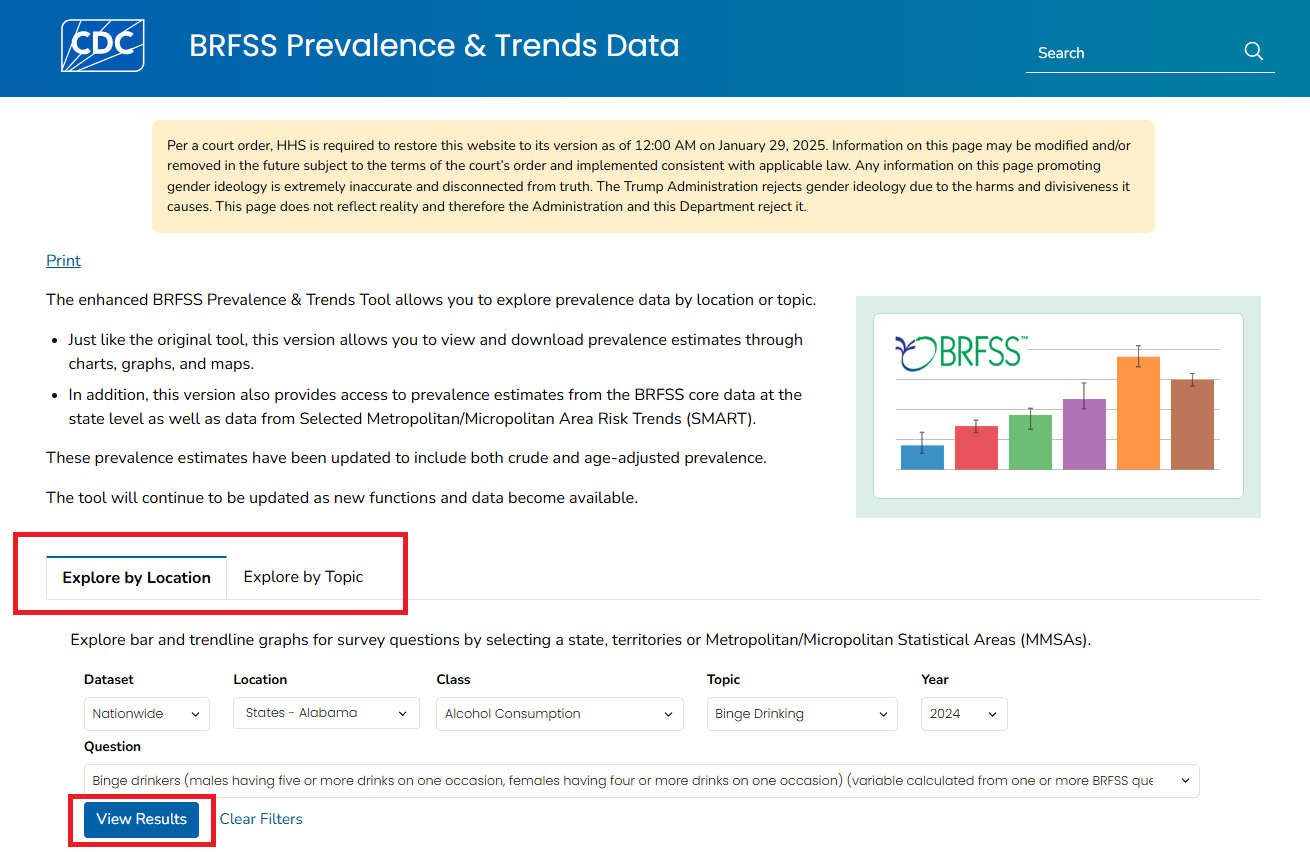
\includegraphics[width=0.9\linewidth,height=\textheight,keepaspectratio]{references/data-sources/../../assets/images/data3/BRFSS12.png}
\end{center}

The results will show the (i) prevalence estimates for alcohol
consumption in Alabama for the year 2024, and (ii) the trend of alcohol
consumption in Alabama over time.

\begin{center}
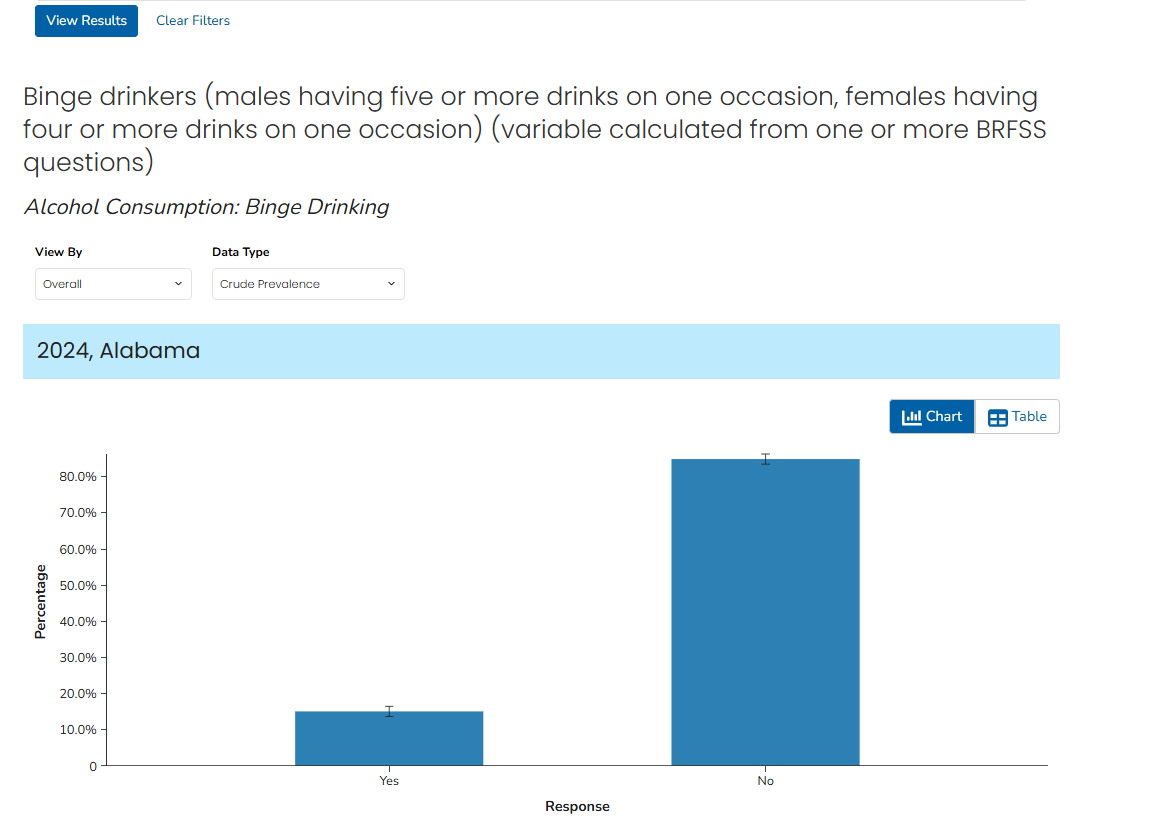
\includegraphics[width=0.9\linewidth,height=\textheight,keepaspectratio]{references/data-sources/../../assets/images/data3/BRFSS13.png}
\end{center}

\begin{center}
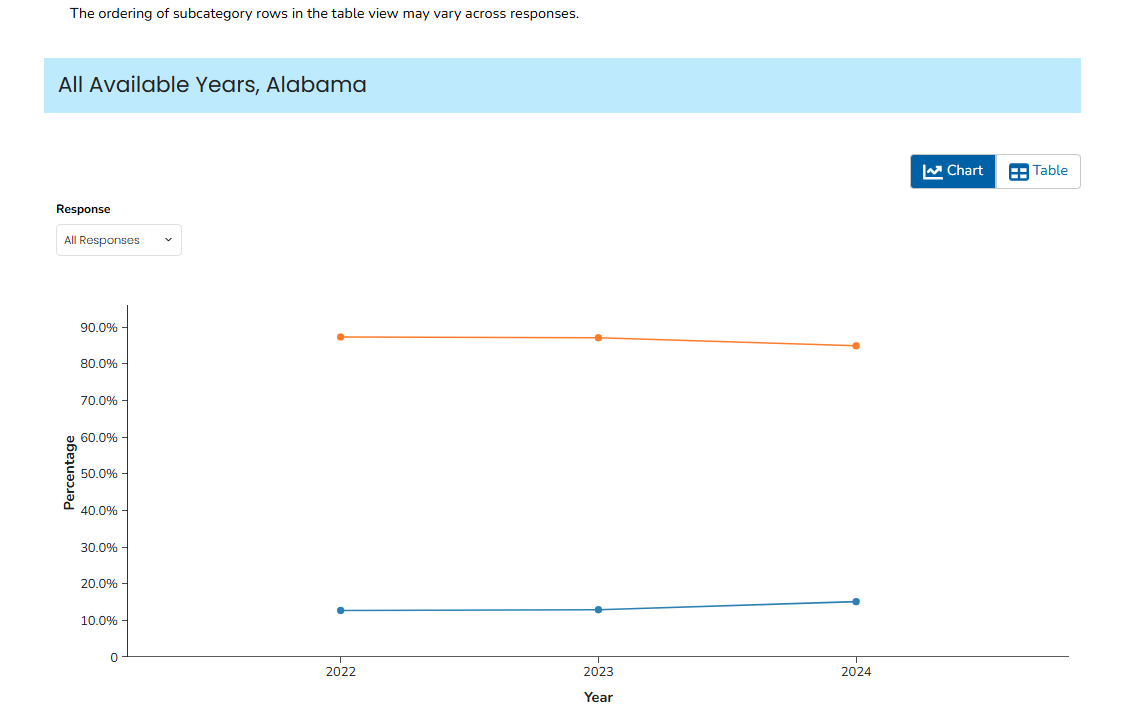
\includegraphics[width=0.9\linewidth,height=\textheight,keepaspectratio]{references/data-sources/../../assets/images/data3/BRFSS14.png}
\end{center}

\chapter*{CCS}\label{ccs}
\addcontentsline{toc}{chapter}{CCS}

\markboth{CCS}{CCS}

The Canadian Cannabis Survey (CCS) is an annual survey conducted by
Health Canada to gather information on cannabis use among people aged 16
years and older living in all Canadian provinces and territories. The
survey collects data on various aspects of cannabis consumption,
including their knowledge, attitudes and behaviours towards cannabis
use.

\begin{center}

\includegraphics[width=0.9\linewidth,height=\textheight,keepaspectratio]{references/data-sources/../../assets/images/data4/ccs1.png}
\end{center}

\marginnote{\begin{footnotesize}

\href{https://open.canada.ca/data/dataset/2abe0796-c3e6-443b-a5c5-74e770e9fbe0}{Health
Canada website for CCS}

\end{footnotesize}}

More than 11,000 respondents participated in the 2024 survey. The study
provides valuable insights into cannabis use patterns, the cannabis
market, and issues of public safety. The survey results are published on
Health Canada's website:

\begin{center}
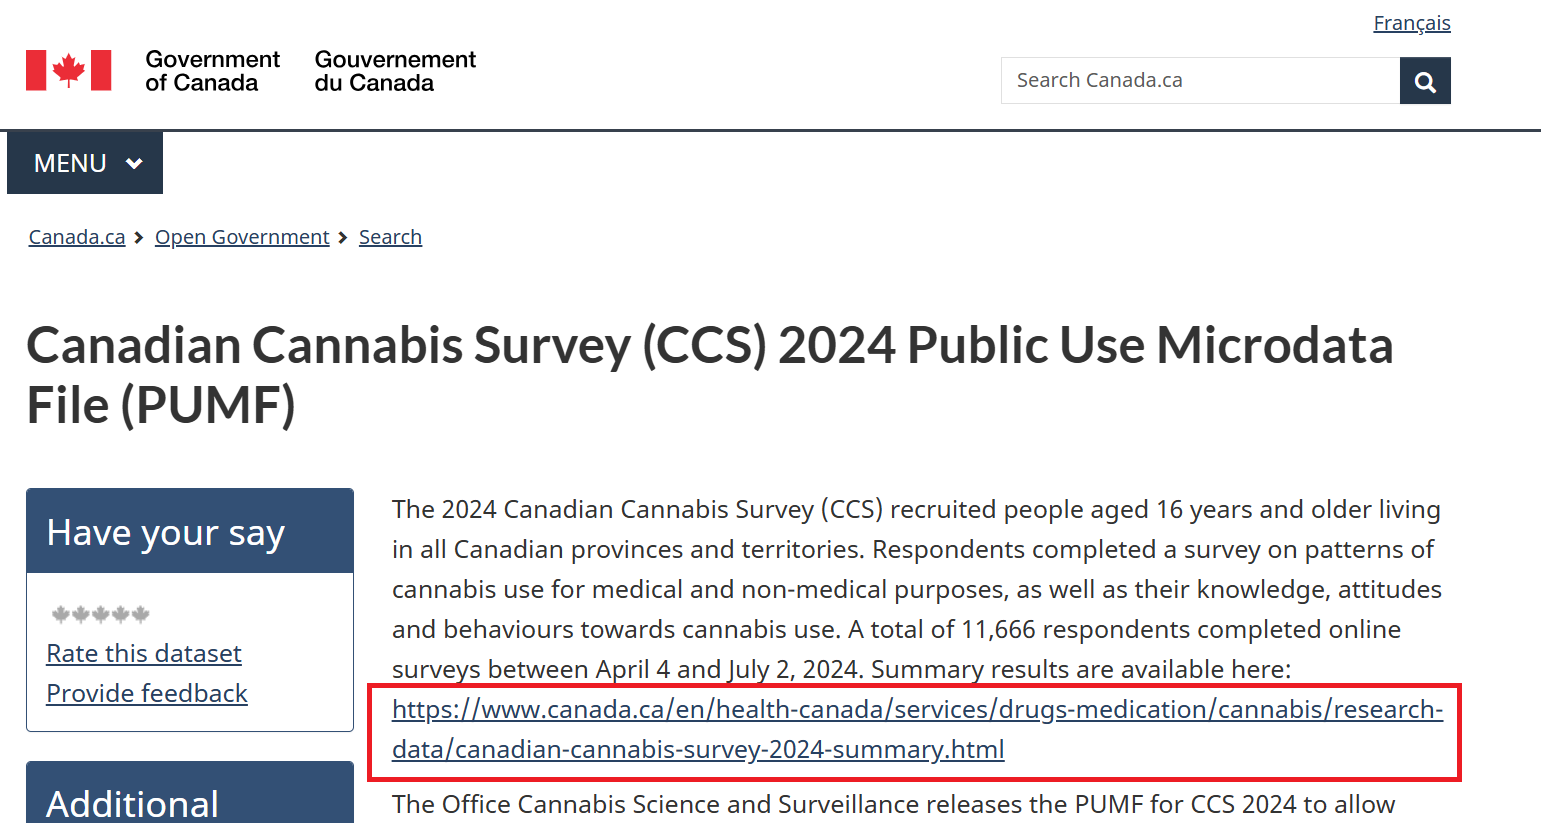
\includegraphics[width=0.9\linewidth,height=\textheight,keepaspectratio]{references/data-sources/../../assets/images/data4/ccs2.png}
\end{center}

\begin{center}

\includegraphics[width=0.9\linewidth,height=\textheight,keepaspectratio]{references/data-sources/../../assets/images/data4/ccs3.png}
\end{center}

\subsection*{Open Licence}\label{open-licence}
\addcontentsline{toc}{subsection}{Open Licence}

The data from the Canadian Cannabis Survey is available under the Open
Government Licence - Canada (OGL-Canada). This licence allows users to
freely use, modify, and distribute the data, provided that they
attribute the source of the data and do not use it for commercial
purposes. The OGL-Canada promotes transparency and encourages the use of
government data for research, analysis, and public benefit. You can
follow the \texttt{Open\ Government\ Licence\ -\ Canada} link for more
information on the terms and conditions of the licence.

\marginnote{\begin{footnotesize}

\href{https://open.canada.ca/en/open-government-licence-canada}{Open
Licence}

\end{footnotesize}}

\begin{center}
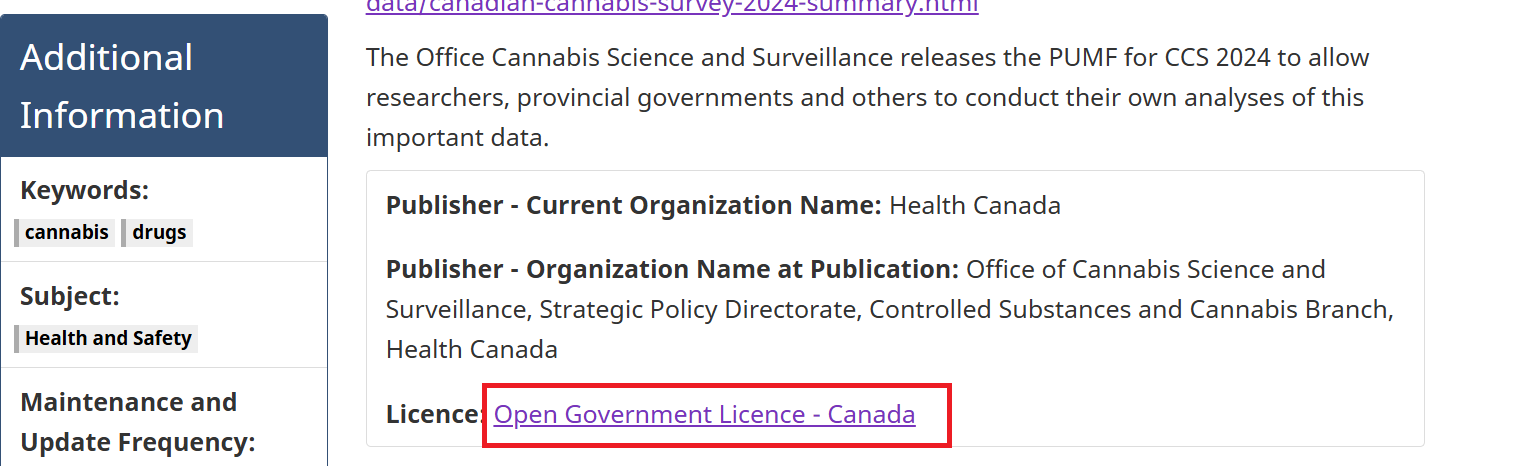
\includegraphics[width=0.9\linewidth,height=\textheight,keepaspectratio]{references/data-sources/../../assets/images/data4/ccs4.png}
\end{center}

\begin{center}

\includegraphics[width=0.9\linewidth,height=\textheight,keepaspectratio]{references/data-sources/../../assets/images/data4/ccs5.png}
\end{center}

\subsection*{Data and Resources}\label{data-and-resources}
\addcontentsline{toc}{subsection}{Data and Resources}

The \texttt{Data\ and\ Resources} tab on the Health Canada website
provides access to the public use data, user guides, and the data
dictionary.

\begin{center}
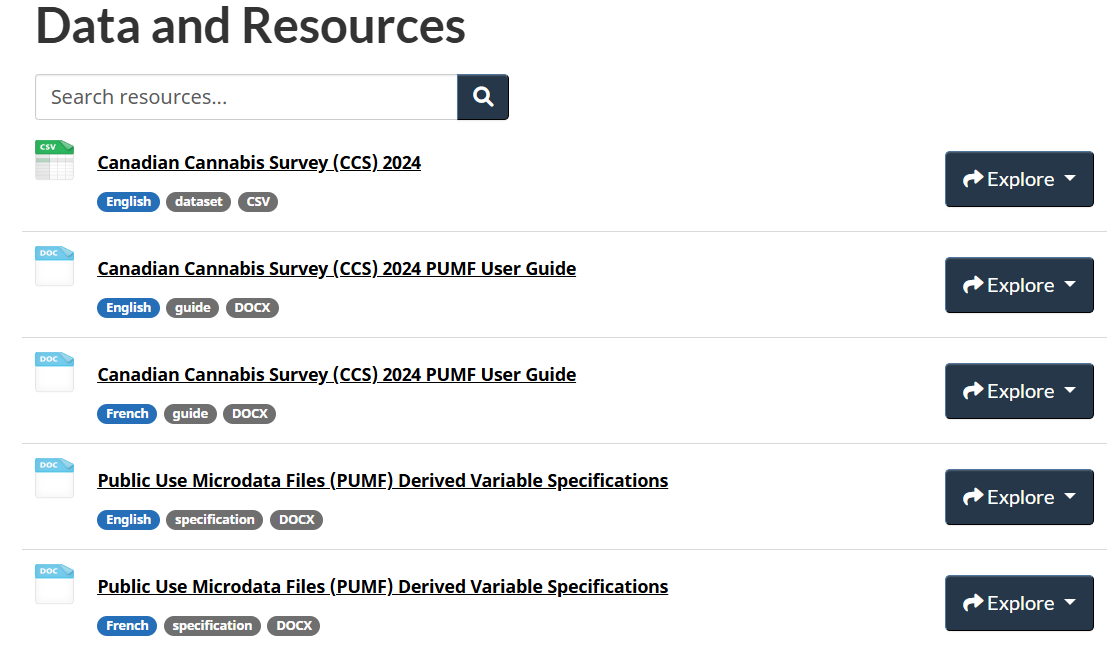
\includegraphics[width=0.9\linewidth,height=\textheight,keepaspectratio]{references/data-sources/../../assets/images/data4/ccs6.png}
\end{center}

The CCS 2024 data is available to download in various formats, including
CSV, TSV, JSON, and XML. The data can be accessed through the Health
Canada website, where you can choose the format that best suits your
needs. You need to open the data link (say, in a new tab in your
browser) and select the desired format to download the data.

\begin{center}
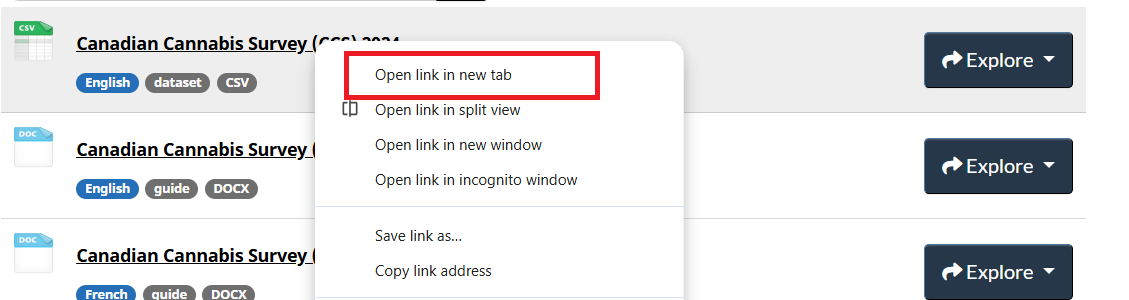
\includegraphics[width=0.9\linewidth,height=\textheight,keepaspectratio]{references/data-sources/../../assets/images/data4/ccs7.png}
\end{center}

Under the \texttt{Download} tab, you can find the data in different
formats. For example, you can download the data in CSV format by
clicking on the \texttt{CSV} link:

\begin{center}
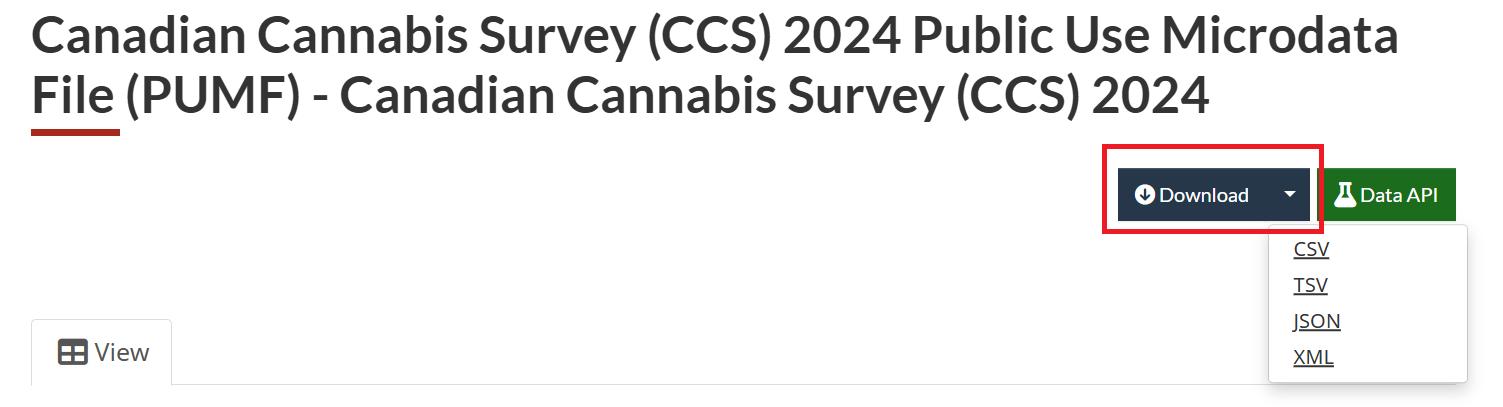
\includegraphics[width=0.9\linewidth,height=\textheight,keepaspectratio]{references/data-sources/../../assets/images/data4/ccs8.png}
\end{center}

After downloading, you can open the data in Excel, Google Sheets, or any
statistical software. The data is structured in a tabular format, with
each row representing an individual respondent and each column
representing different variables:

\begin{center}
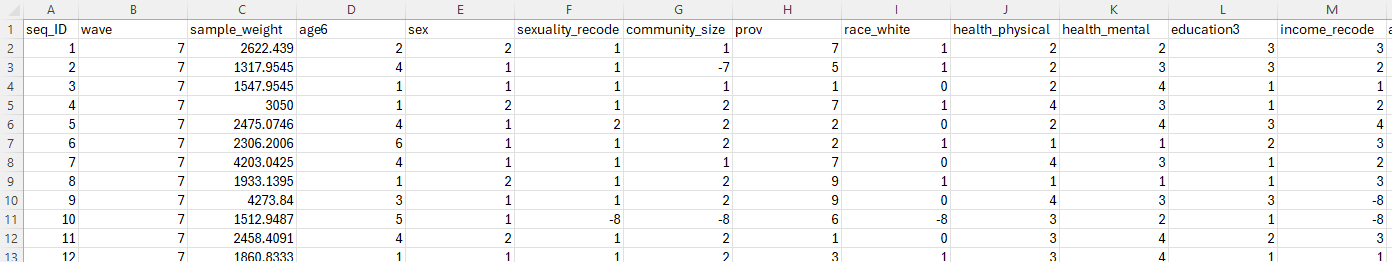
\includegraphics[width=0.9\linewidth,height=\textheight,keepaspectratio]{references/data-sources/../../assets/images/data4/ccs9.png}
\end{center}

The \texttt{Canadian\ Cannabis\ Survey\ (CCS)\ 2024\ PUMF\ User\ Guide}
gives detailed information on the survey methodology, data collection
process, and how to use the public use microdata file (PUMF). You can
also find the variable names and their descriptions in this file.

\marginnote{\begin{footnotesize}

\href{https://open.canada.ca/data/dataset/2abe0796-c3e6-443b-a5c5-74e770e9fbe0/resource/0629eaec-7ba7-492d-9322-d20dc80e55d8}{2024
Public Use Microdata File}

\end{footnotesize}}

\begin{center}
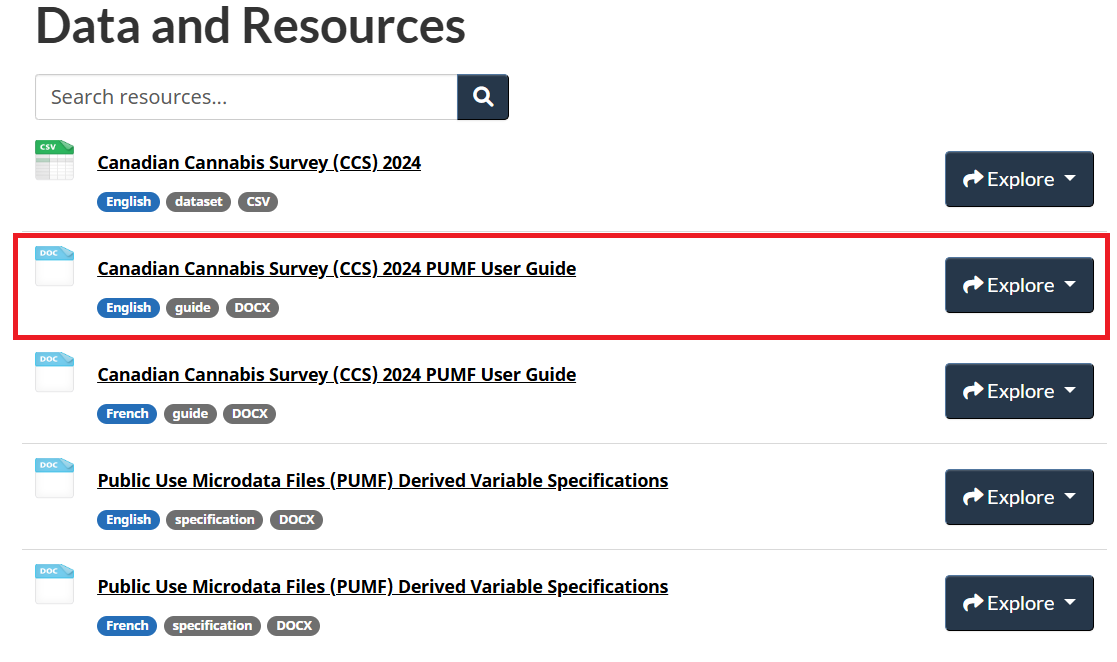
\includegraphics[width=0.9\linewidth,height=\textheight,keepaspectratio]{references/data-sources/../../assets/images/data4/ccs10.png}
\end{center}

Let's find a variable (\texttt{access\_ease\_legal}) in the Excel file
and check its description in the data dictionary. You can use the
\texttt{Find} function in Excel (\texttt{Ctrl\ +\ F}) to search for the
variable name:

\begin{center}
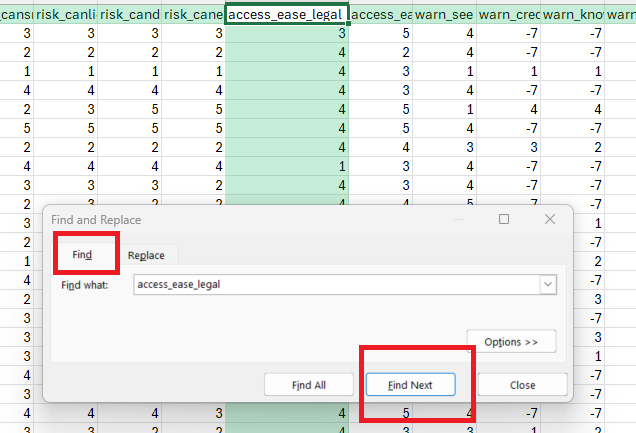
\includegraphics[width=0.9\linewidth,height=\textheight,keepaspectratio]{references/data-sources/../../assets/images/data4/ccs11.png}
\end{center}

Then you can see the description of the variable in the
\texttt{Canadian\ Cannabis\ Survey\ (CCS)\ 2024\ PUMF\ User\ Guide},
which provides information on what the variable represents and how it
was coded:

\begin{center}
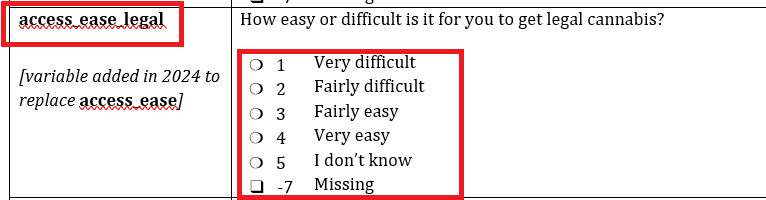
\includegraphics[width=0.9\linewidth,height=\textheight,keepaspectratio]{references/data-sources/../../assets/images/data4/ccs12.png}
\end{center}

In this dataset, \texttt{-7} generally represents missing. Always check
the data dictionary for the specific coding of missing values, ``don't
know,'' or ``refused'' responses, as they can vary between datasets.

\chapter*{CADS}\label{cads}
\addcontentsline{toc}{chapter}{CADS}

\markboth{CADS}{CADS}

The Canadian Alcohol and Drugs Survey (CADS) is a national survey
conducted by Statistics Canada that collects data on the use of
substances, such as alcohol, cannabis and other drugs. The study was
conducted by Statistics Canada in 2019 with the cooperation and support
of Health Canada. The target population for the survey was all persons
aged 15 years and over living in Canada, excluding residents of the
Yukon, Northwest Territories, and Nunavut, full-time residents of
institutions, and residents of Native reserves.

\begin{center}

\includegraphics[width=0.9\linewidth,height=\textheight,keepaspectratio]{references/data-sources/../../assets/images/data5/cads1.png}
\end{center}

\marginnote{\begin{footnotesize}

\href{https://ouvert.canada.ca/data/dataset/5c1d47e4-d2be-49d9-9a23-c38f79490fad}{Health
Canada website for CADS}

\end{footnotesize}}

\marginnote{\begin{footnotesize}

\href{https://www.canada.ca/en/health-canada/services/canadian-alcohol-drugs-survey/2019-summary.html}{CADS
2019 summary of results}

\end{footnotesize}}

\subsection*{Open Licence}\label{open-licence-1}
\addcontentsline{toc}{subsection}{Open Licence}

Similar to the
\href{https://open.canada.ca/data/dataset/2abe0796-c3e6-443b-a5c5-74e770e9fbe0}{Canadian
Cannabis Survey}, the CADS is also licensed under the
\href{https://open.canada.ca/en/open-government-licence-canada}{Open
Government Licence - Canada}. This means that the data can be freely
used, modified, and shared by anyone for any purpose, as long as they
provide proper attribution to the source of the data.

\begin{center}
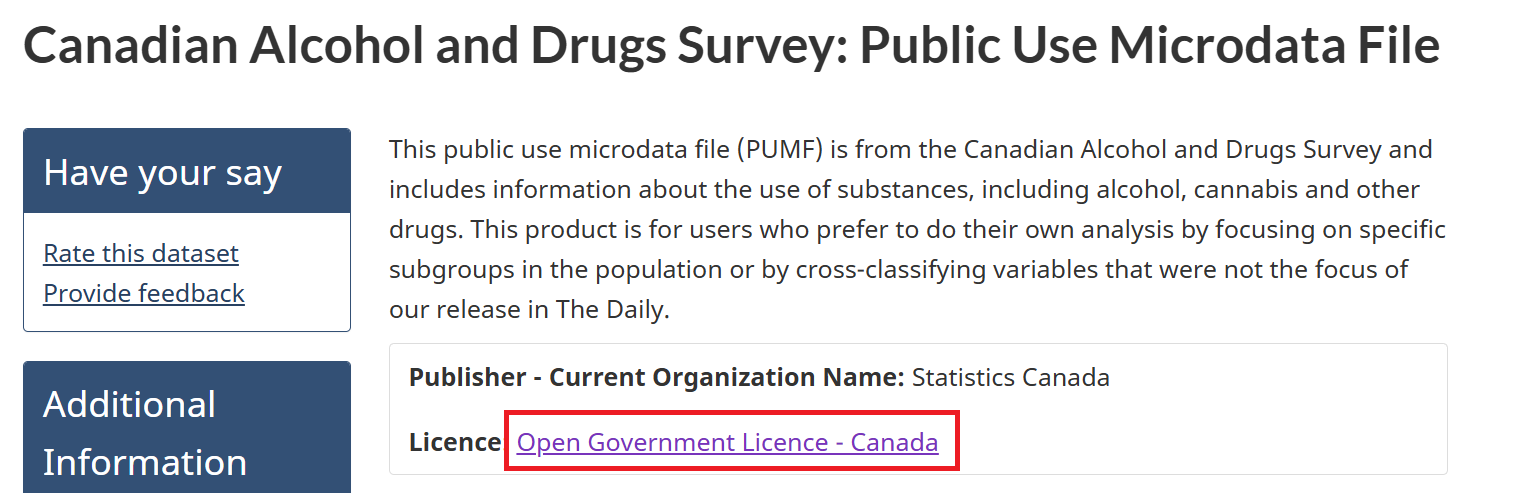
\includegraphics[width=0.9\linewidth,height=\textheight,keepaspectratio]{references/data-sources/../../assets/images/data5/cads2.png}
\end{center}

\begin{center}

\includegraphics[width=0.9\linewidth,height=\textheight,keepaspectratio]{references/data-sources/../../assets/images/data5/cads3.png}
\end{center}

\subsection*{Data and Resources}\label{data-and-resources-1}
\addcontentsline{toc}{subsection}{Data and Resources}

The \texttt{Data\ and\ Resources} tab provides access to the public use
data, user guides, and the data dictionary.

\begin{center}
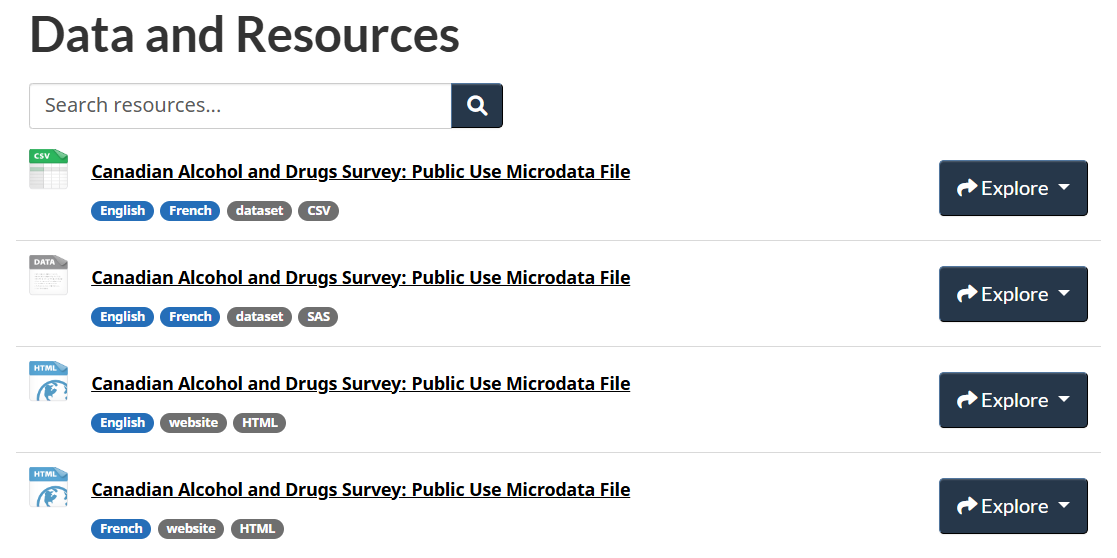
\includegraphics[width=0.9\linewidth,height=\textheight,keepaspectratio]{references/data-sources/../../assets/images/data5/cads4.png}
\end{center}

The public use data file is available in a ZIP format. You need to open
the
\texttt{Canadian\ Alcohol\ and\ Drugs\ Survey:\ Public\ Use\ Microdata\ File}
link, and click on \texttt{Go\ to\ resource}to download the ZIP file.

\begin{center}
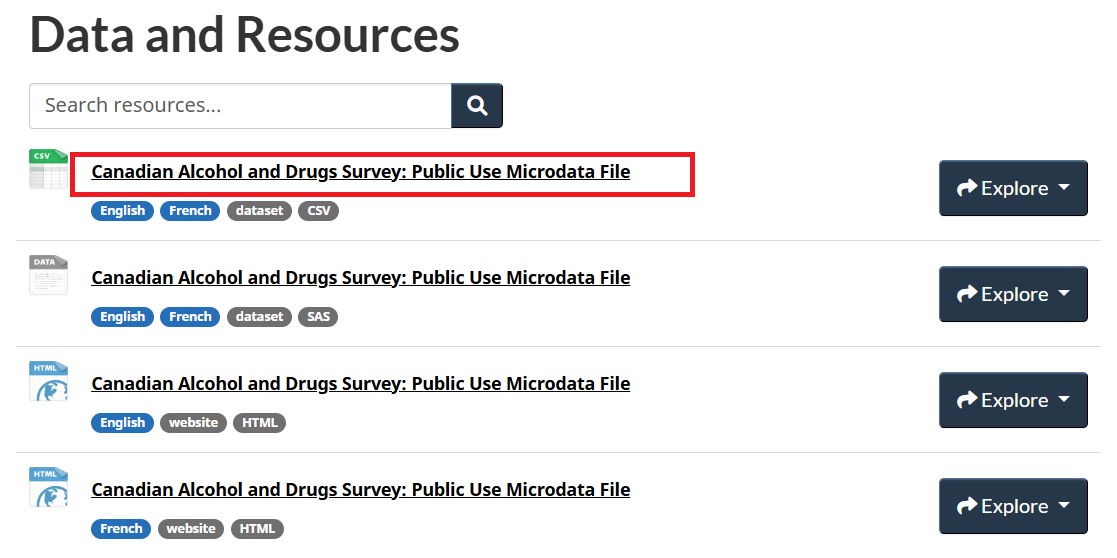
\includegraphics[width=0.9\linewidth,height=\textheight,keepaspectratio]{references/data-sources/../../assets/images/data5/cads5.png}
\end{center}

\begin{center}

\includegraphics[width=0.9\linewidth,height=\textheight,keepaspectratio]{references/data-sources/../../assets/images/data5/cads6.png}
\end{center}

The ZIP file contains the following files: an instruction on how to cite
CADS 2019, data documentation, and the dataset in CSV format.

\begin{center}
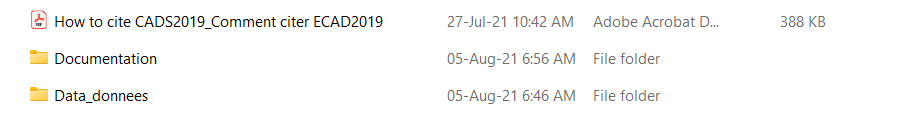
\includegraphics[width=0.9\linewidth,height=\textheight,keepaspectratio]{references/data-sources/../../assets/images/data5/cads7.png}
\end{center}

\subsection*{Data Documentation}\label{data-documentation}
\addcontentsline{toc}{subsection}{Data Documentation}

The data documentation folder includes three sub-folders:
\texttt{Codebook\_Livre\ des\ codes}, \texttt{Guide}, and
\texttt{Questionnaires}.

\begin{center}
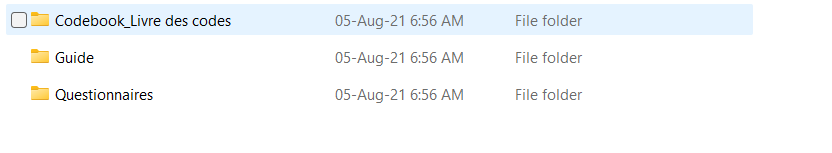
\includegraphics[width=0.9\linewidth,height=\textheight,keepaspectratio]{references/data-sources/../../assets/images/data5/cads8.png}
\end{center}

The \texttt{Guide} folder contains user guides (in English and French)
that provide an overview of the survey, including the methodology, data
collection process, data processing, data quality, and sampling weights.

\begin{center}
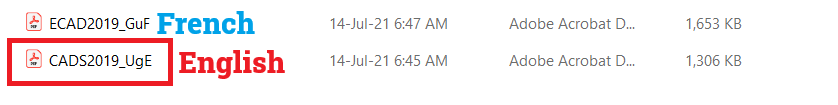
\includegraphics[width=0.9\linewidth,height=\textheight,keepaspectratio]{references/data-sources/../../assets/images/data5/cads9.png}
\end{center}

The \texttt{Codebook\_Livre\ des\ codes} folder contains codebooks (in
English and French) that provide detailed information about the
variables in the dataset, including variable names, labels, and values.
There are two types of codebooks: those with and those without variable
frequencies. But both codebooks provide the same information about the
variables in the dataset.

\begin{center}
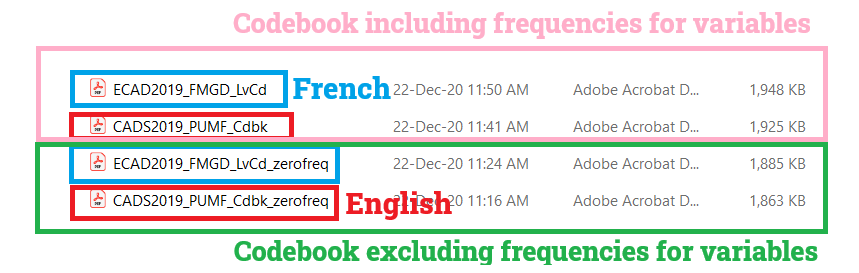
\includegraphics[width=0.9\linewidth,height=\textheight,keepaspectratio]{references/data-sources/../../assets/images/data5/cads10.png}
\end{center}

The \texttt{Questionnaires} folder contains the survey questionnaires
(in English and French) that were used to collect the data.

\subsection*{Data}\label{data-1}
\addcontentsline{toc}{subsection}{Data}

The \texttt{Data\_donnees} folder contains the dataset in CSV format.
You can open the dataset in Excel or any statistical software to explore
the data. The row represents the respondent, and the column represents
the variable:

\begin{center}
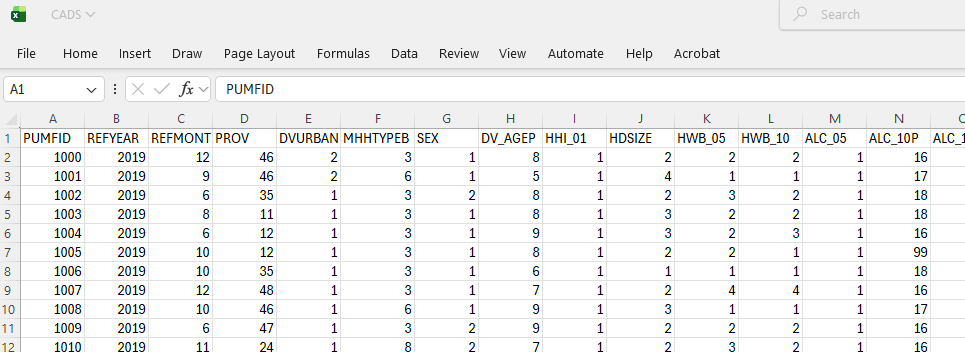
\includegraphics[width=0.9\linewidth,height=\textheight,keepaspectratio]{references/data-sources/../../assets/images/data5/cads11.png}
\end{center}

You can refer to the codebook to understand the variables that you are
interested in for your analysis. For example, if you are interested in
the variable \texttt{DVURBAN}, you can refer to the codebook to find out
that the variable (e.g., for the English version of the codebook with
frequencies):

\begin{center}
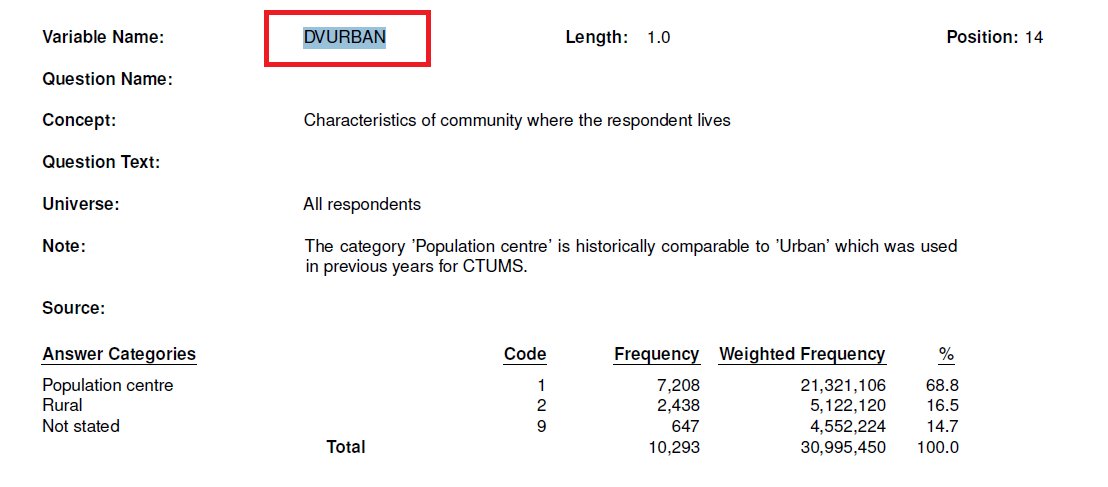
\includegraphics[width=0.9\linewidth,height=\textheight,keepaspectratio]{references/data-sources/../../assets/images/data5/cads12.png}
\end{center}

\chapter*{CTNS}\label{ctns}
\addcontentsline{toc}{chapter}{CTNS}

\markboth{CTNS}{CTNS}

The Canadian Tobacco and Nicotine Survey (CTNS) is a cross-sectional
survey that collects information on tobacco and nicotine use among
Canadians aged 15 years and older. The survey is conducted by Statistics
Canada on behalf of Health Canada and provides valuable insights into
the prevalence of cigarette smoking, vaping, cannabis, and alcohol use.

\begin{center}

\includegraphics[width=0.9\linewidth,height=\textheight,keepaspectratio]{references/data-sources/../../assets/images/data6/ctns1.png}
\end{center}

\marginnote{\begin{footnotesize}

\href{https://open.canada.ca/data/en/dataset/7147c035-4418-499c-9623-a0584debfcb1}{Health
Canada website for CTNS}

\end{footnotesize}}

\marginnote{\begin{footnotesize}

\href{https://www.canada.ca/en/health-canada/services/canadian-tobacco-nicotine-survey/2022-summary.html}{CTNS
2022 summary of results}

\end{footnotesize}}

\subsection*{Open Licence}\label{open-licence-2}
\addcontentsline{toc}{subsection}{Open Licence}

The CTNS is licensed under the
\href{https://open.canada.ca/en/open-government-licence-canada}{Open
Government Licence - Canada}. This means that the data can be freely
used, modified, and shared by anyone for any purpose, as long as they
provide proper attribution to the source of the data.

\subsection*{Data and Resources}\label{data-and-resources-2}
\addcontentsline{toc}{subsection}{Data and Resources}

The \texttt{Data\ and\ Resources} tab provides access to the public use
data, user guides, and the data dictionary.

\begin{center}
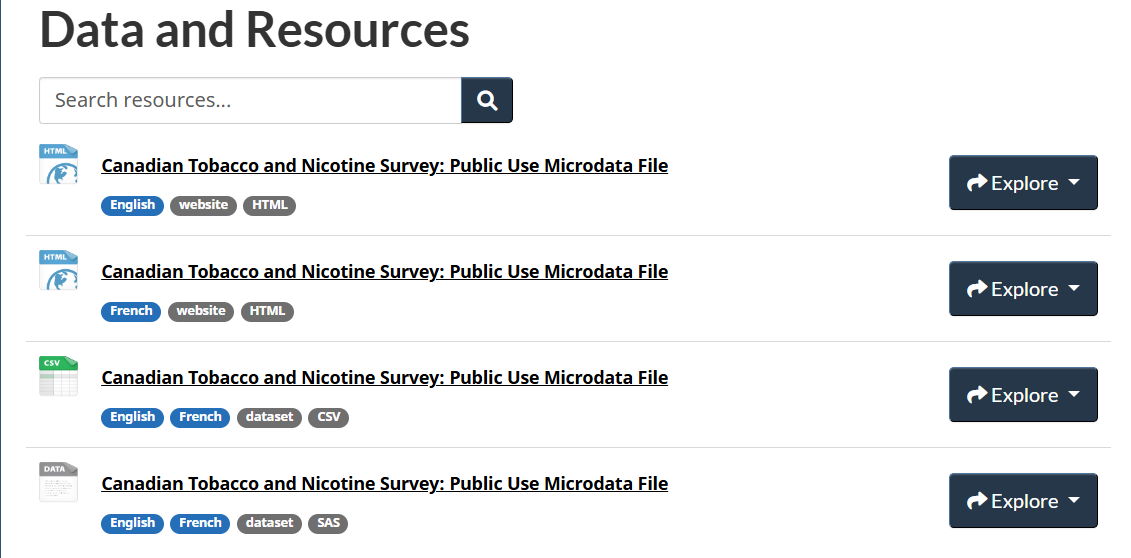
\includegraphics[width=0.9\linewidth,height=\textheight,keepaspectratio]{references/data-sources/../../assets/images/data6/ctns2.png}
\end{center}

The public use data file is available in a ZIP format. You can click on
the
\texttt{Canadian\ Tobacco\ and\ Nicotine\ Survey:\ Public\ Use\ Microdata\ File}
link, followed by \texttt{Go\ to\ resource} link to download the ZIP
file.

\begin{center}
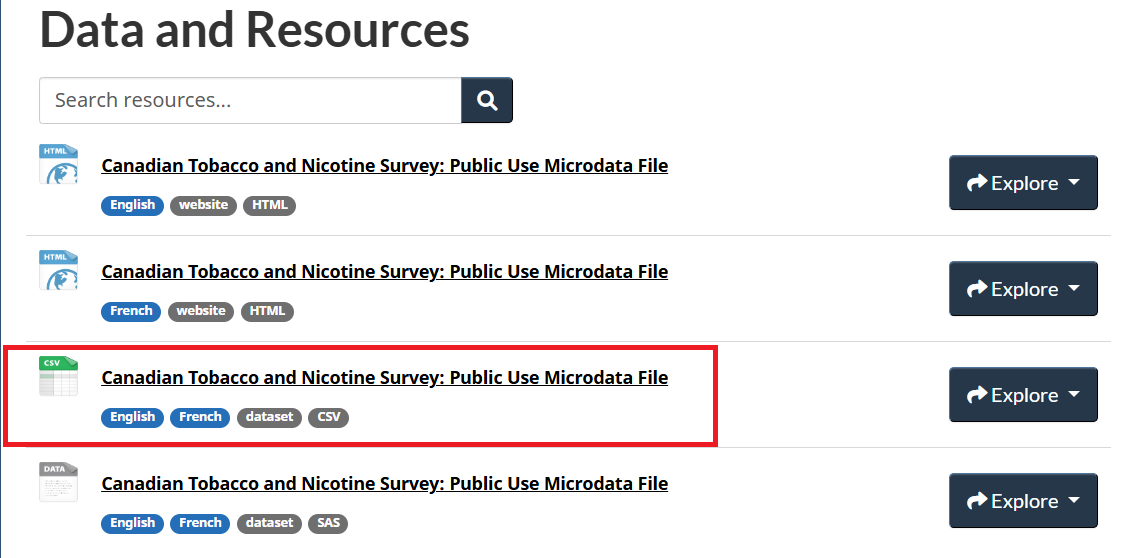
\includegraphics[width=0.9\linewidth,height=\textheight,keepaspectratio]{references/data-sources/../../assets/images/data6/ctns3.png}
\end{center}

\begin{center}

\includegraphics[width=0.9\linewidth,height=\textheight,keepaspectratio]{references/data-sources/../../assets/images/data6/ctns4.png}
\end{center}

Similar to the \href{data5.html}{Canadian Alcohol and Drugs Survey
(CADS)} tutorial, the ZIP file for CTNS contains the following files:
citation instructions, data documentation, and the dataset in CSV
format. The data documentation, questionnaire, and codebook are also the
same as those for CADS. The only difference is that the data
documentation and questionnaire for CTNS are labelled \texttt{CTNS}
rather than \texttt{CADS}.

\chapter*{CSADS}\label{csads}
\addcontentsline{toc}{chapter}{CSADS}

\markboth{CSADS}{CSADS}

The Canadian Student Alcohol and Drugs Survey (CSADS) is a national
survey that collects data on the alcohol and drug use patterns of
Canadian students in grades 7 to 12. The survey is conducted every two
years and provides valuable insights into the prevalence and trends of
substance use among Canadian youth.

\begin{center}

\includegraphics[width=0.9\linewidth,height=\textheight,keepaspectratio]{references/data-sources/../../assets/images/data7/csads1.png}
\end{center}

\marginnote{\begin{footnotesize}

\href{https://open.canada.ca/data/en/dataset/7147c035-4418-499c-9623-a0584debfcb1}{Health
Canada website for CTNS}

\end{footnotesize}}

\marginnote{\begin{footnotesize}

\href{https://www.canada.ca/en/health-canada/services/canadian-student-tobacco-alcohol-drugs-survey.html}{CSADS
summary of results}

\end{footnotesize}}

\subsection*{Open Licence}\label{open-licence-3}
\addcontentsline{toc}{subsection}{Open Licence}

The CTNS is licensed under the
\href{https://open.canada.ca/en/open-government-licence-canada}{Open
Government Licence - Canada}. This means that the data can be freely
used, modified, and shared by anyone for any purpose, as long as they
provide proper attribution to the source of the data.

\subsection*{Data and Resources}\label{data-and-resources-3}
\addcontentsline{toc}{subsection}{Data and Resources}

The \texttt{Data\ and\ Resources} tab provides access to the public use
data, user guides, the data dictionary, and information on bootstrap
weights.

\begin{center}
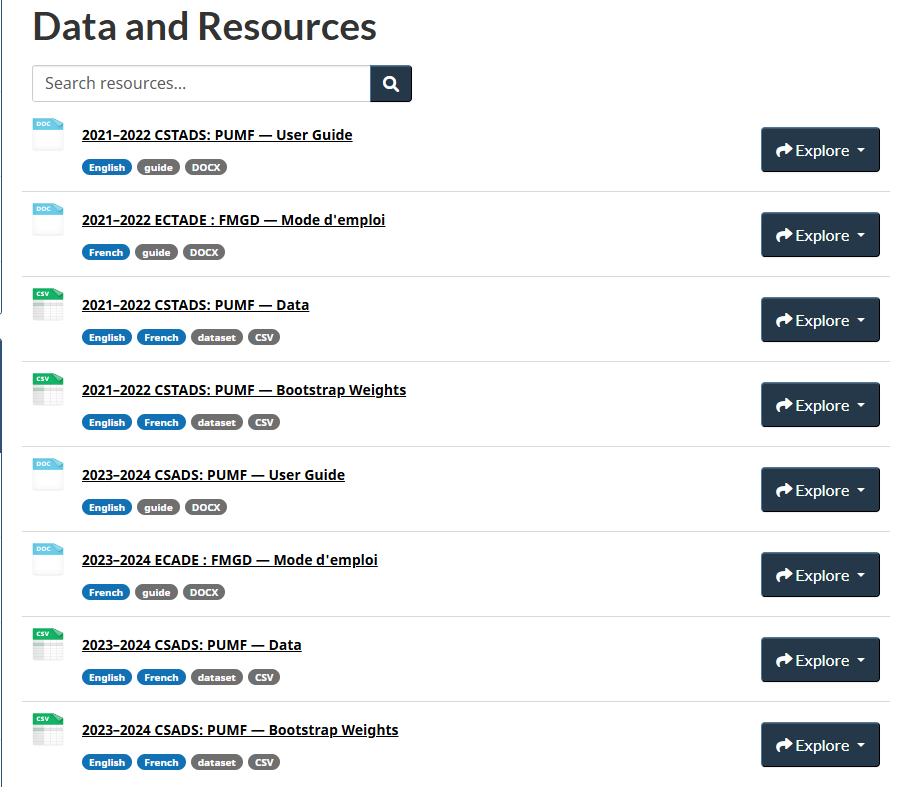
\includegraphics[width=0.9\linewidth,height=\textheight,keepaspectratio]{references/data-sources/../../assets/images/data7/csads2.png}
\end{center}

To download the 2021--2022 CSTADS, you can click on the
\texttt{2021–2022\ CSTADS:\ PUMF\ —\ Dataset\ in\ CSV\ format} link. The
data is available to download in various formats. Under the
\texttt{Download} tab, you can find the formats. For example, you can
download the data in CSV format by clicking on the \texttt{CSV} link:

\begin{center}

\includegraphics[width=0.9\linewidth,height=\textheight,keepaspectratio]{references/data-sources/../../assets/images/data7/csads3.png}
\end{center}

After downloading, you can open the data in Excel, Google Sheets, or any
statistical software. The data is structured in a tabular format, with
each row representing an individual respondent and each column
representing different variables:

\begin{center}
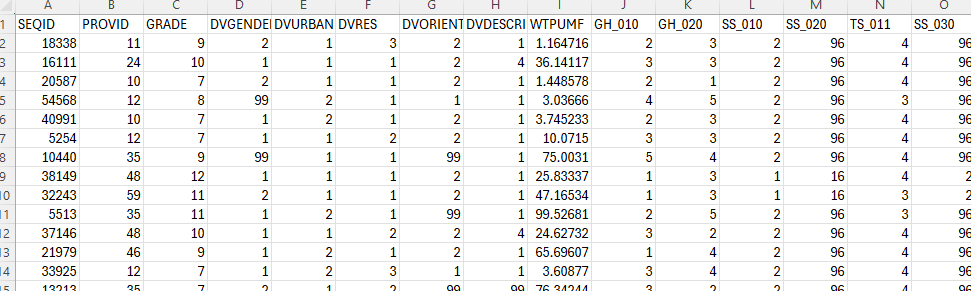
\includegraphics[width=0.9\linewidth,height=\textheight,keepaspectratio]{references/data-sources/../../assets/images/data7/csads4.png}
\end{center}

The user guide gives detailed information on the survey methodology,
data collection process, and how to use the public use microdata file
(PUMF). You can also find the variable names and their descriptions in
this \texttt{DOCX} file.

\begin{center}
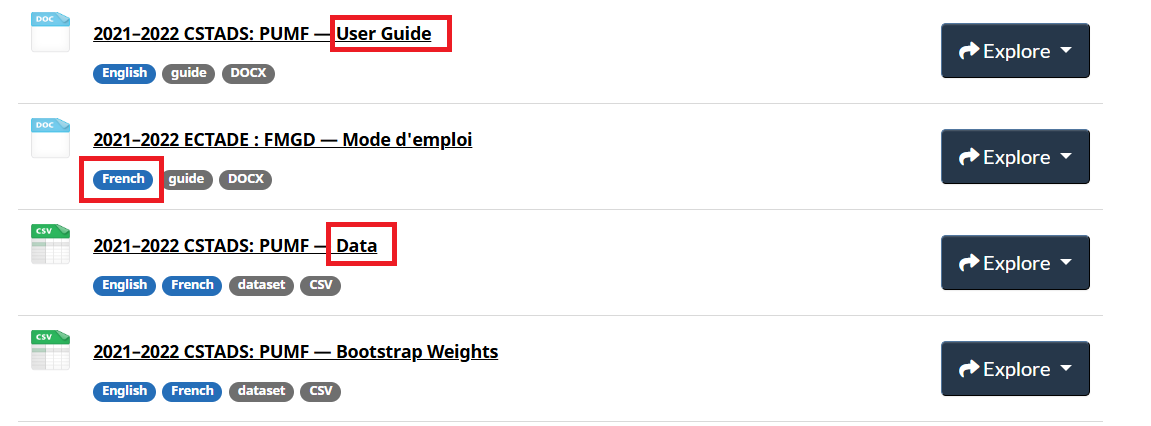
\includegraphics[width=0.9\linewidth,height=\textheight,keepaspectratio]{references/data-sources/../../assets/images/data7/csads5.png}
\end{center}

\begin{center}

\includegraphics[width=0.9\linewidth,height=\textheight,keepaspectratio]{references/data-sources/../../assets/images/data7/csads6.png}
\end{center}

\begin{center}

\includegraphics[width=0.9\linewidth,height=\textheight,keepaspectratio]{references/data-sources/../../assets/images/data7/csads7.png}
\end{center}

To find a variable description, you are referred to the
\texttt{User\ Guide}. For example, the variable \texttt{GH\_010} is
described as follows:

\begin{center}
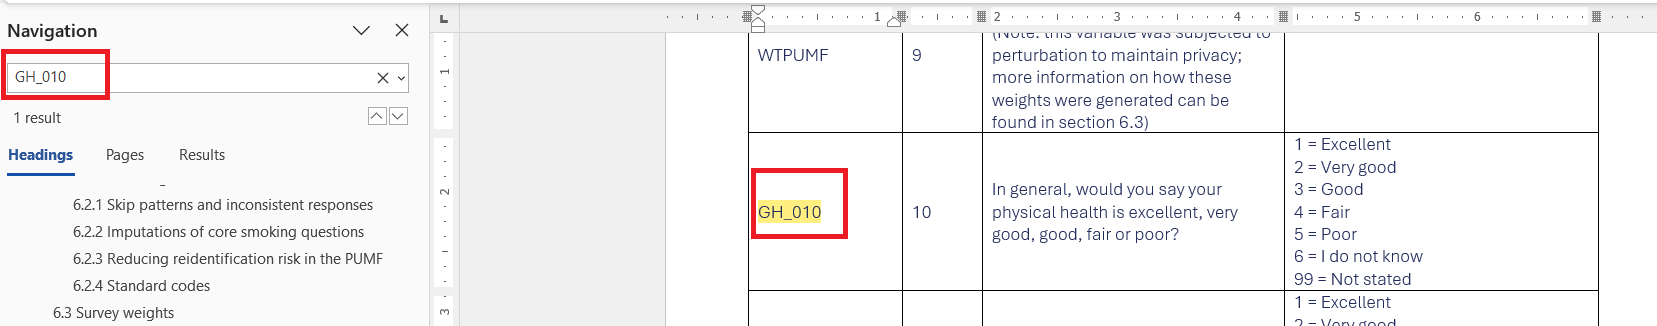
\includegraphics[width=0.9\linewidth,height=\textheight,keepaspectratio]{references/data-sources/../../assets/images/data7/csads8.png}
\end{center}

\chapter*{PHAC Health Infobase}\label{phac-health-infobase}
\addcontentsline{toc}{chapter}{PHAC Health Infobase}

\markboth{PHAC Health Infobase}{PHAC Health Infobase}

The Health Infobase is a comprehensive digital platform maintained by
the Public Health Agency of Canada (PHAC). The Infobase provides access
to a wide range of health-related data tools, infographics, charts and
blogs. There are 182 data sources available on the Infobase. The Health
Infobase serves as a central hub for national surveillance data,
interactive data tools, and public health reports. The platform is
frequently updated with the latest surveillance data.

\begin{center}

\includegraphics[width=0.9\linewidth,height=\textheight,keepaspectratio]{references/data-sources/../../assets/images/data8/infobase1.png}
\end{center}

\marginnote{\begin{footnotesize}

\href{https://health-infobase.canada.ca/}{PHAC Health Infobase}

\end{footnotesize}}

\subsection*{Data Categories}\label{data-categories}
\addcontentsline{toc}{subsection}{Data Categories}

The Infobase provides access to health data under six categories:

\begin{itemize}
\item
  \texttt{Diseases\ and\ disorders}: Comprehensive tracking of chronic
  conditions such as cancer, cardiovascular diseases, and COVID-19.
\item
  \texttt{Drugs\ and\ vaccines}: Data on prescription drugs, vaccine
  coverage, and immunization rates across the country. `
\item
  \texttt{Mental\ health,\ healthy\ living\ and\ environment}:
  Information on mental health indicators, physical activity levels,
  nutrition, and environmental factors such as wildfires.
\item
  \texttt{Injuries\ and\ death}: Data on death, suicide, violence, and
  drowning across regions.
\item
  \texttt{Population\ groups\ and\ demography}: Data on birth,
  maternity, children, family, and disabilities.
\item
  \texttt{Substance\ use}: Data on substance use such as alcohol,
  cannabis use, opioids, and smoking.
\end{itemize}

Under each category, users can select the data for specific health
topics. The three top categories are \texttt{Respiratory\ diseases},
\texttt{Opioids} and \texttt{Mental\ health}.

\begin{center}
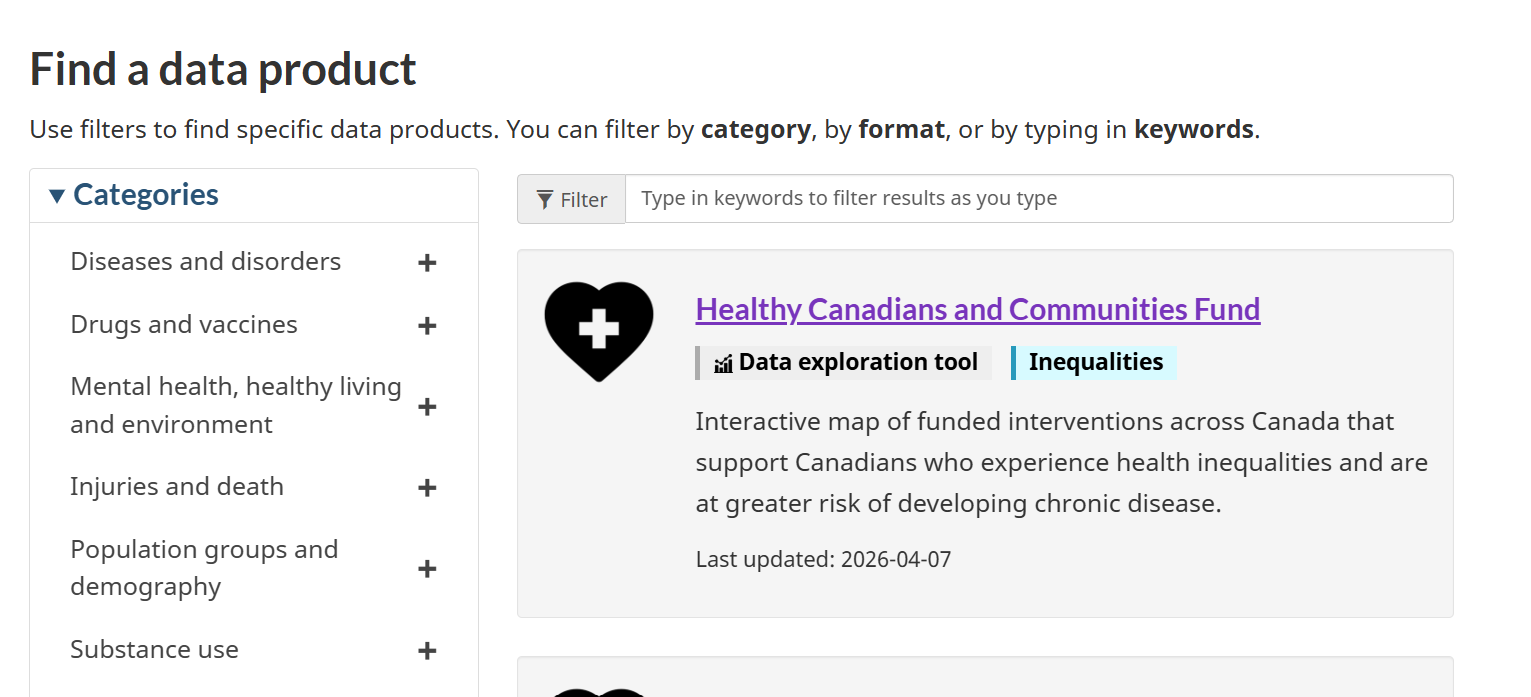
\includegraphics[width=0.9\linewidth,height=\textheight,keepaspectratio]{references/data-sources/../../assets/images/data8/infobase2.png}
\end{center}

\begin{center}
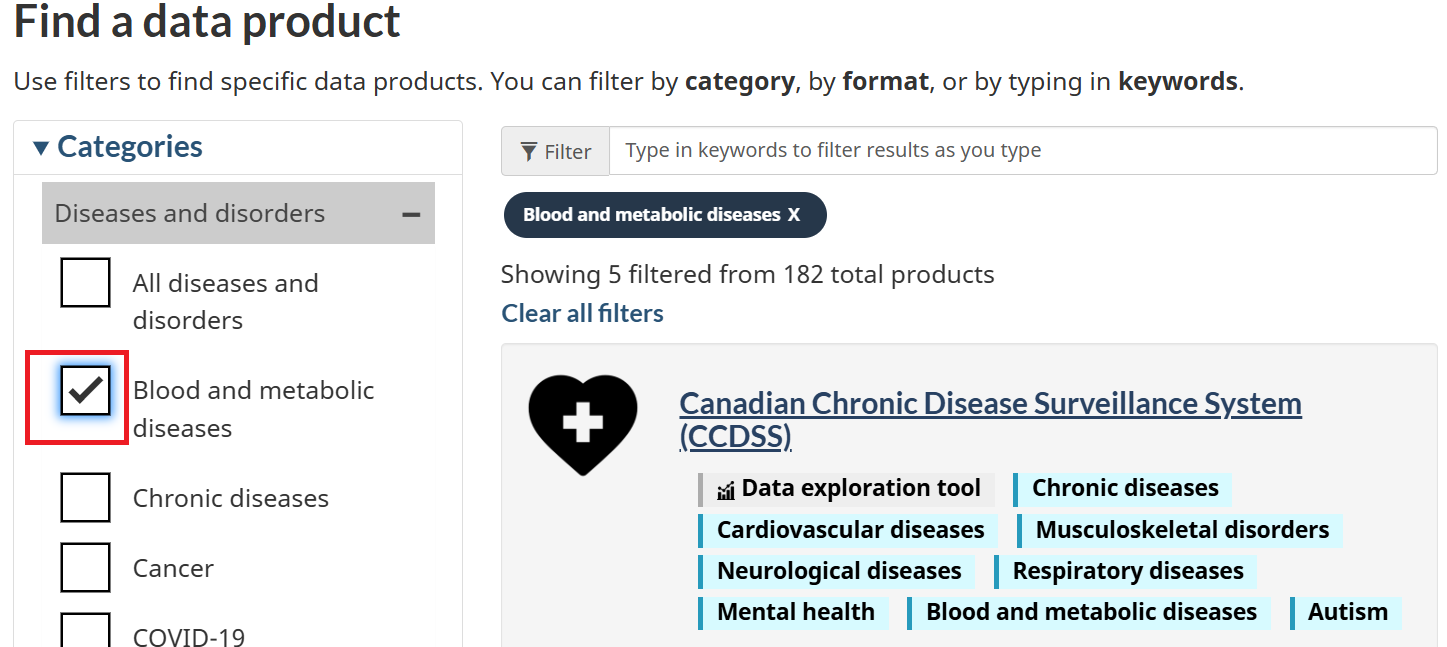
\includegraphics[width=0.9\linewidth,height=\textheight,keepaspectratio]{references/data-sources/../../assets/images/data8/infobase3.png}
\end{center}

You can filter the data by category, by format, or by typing in
keywords.

\begin{center}
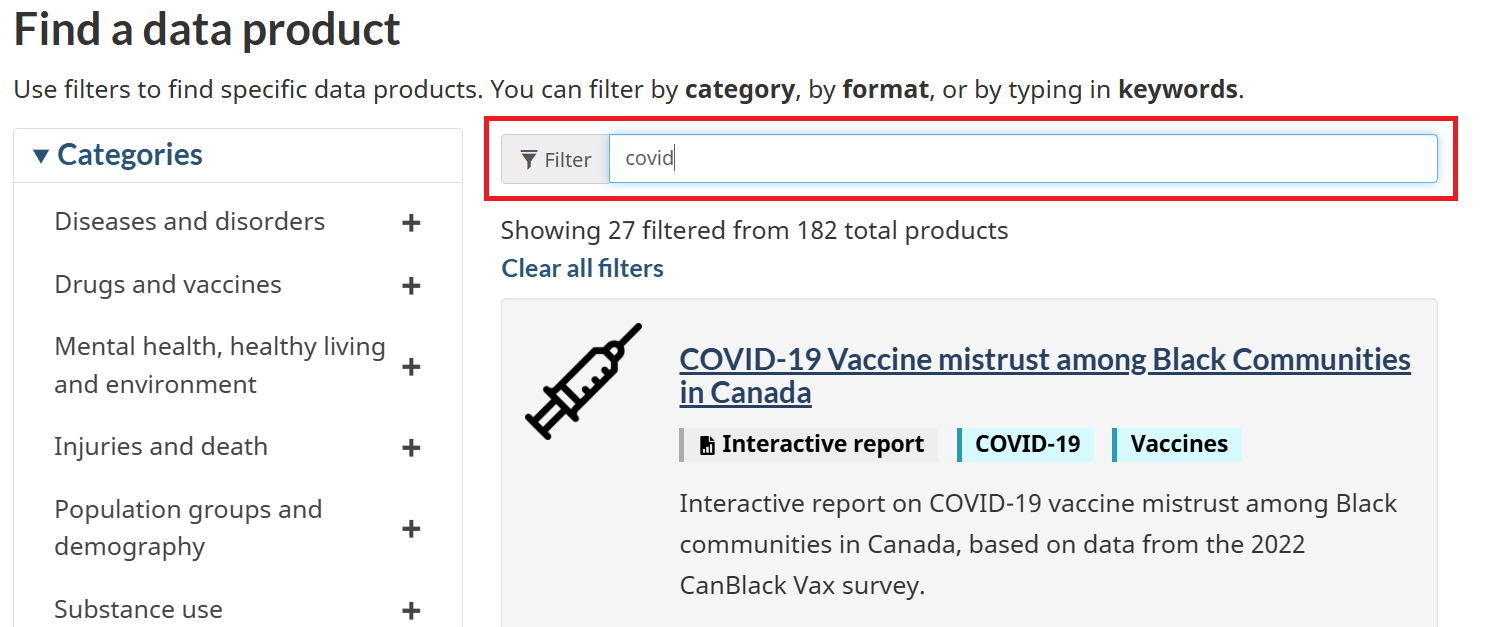
\includegraphics[width=0.9\linewidth,height=\textheight,keepaspectratio]{references/data-sources/../../assets/images/data8/infobase4.png}
\end{center}

You can also filter the data by type, such as blog, infographic, or
report.

\begin{center}
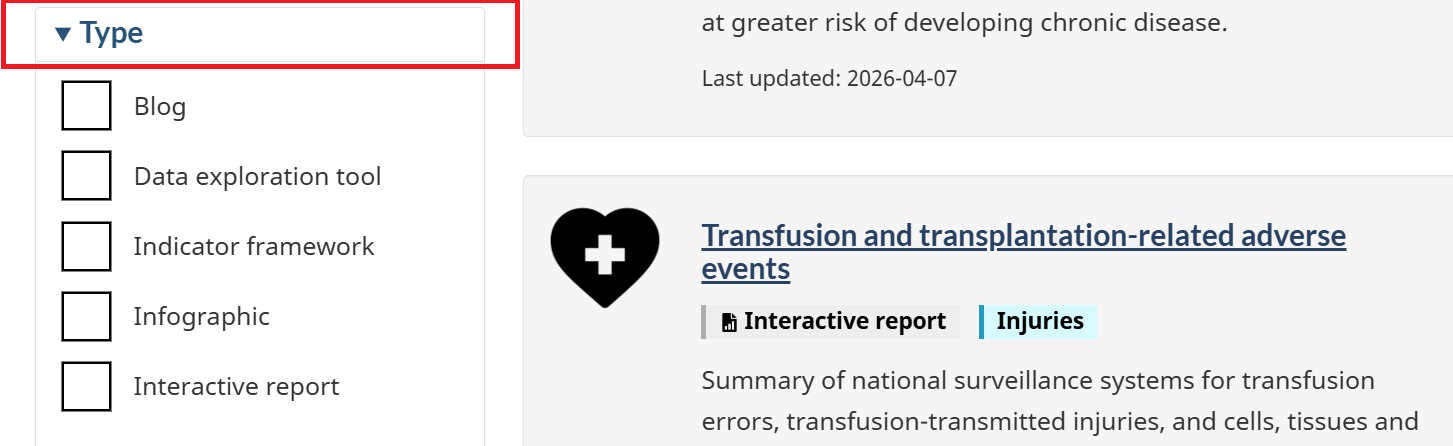
\includegraphics[width=0.9\linewidth,height=\textheight,keepaspectratio]{references/data-sources/../../assets/images/data8/infobase5.png}
\end{center}

\subsection*{Data Availability}\label{data-availability}
\addcontentsline{toc}{subsection}{Data Availability}

The level of information provided in the data sources varies. For some
data sources/products, you can find blogs, infographics, and reports
along with individual-level data. However, for some data
sources/products, you may only find the summary statistics without
individual-level data, i.e., only aggregated-level data. For example,
the \texttt{Human\ Papillomavirus\ Indicator\ Framework} product
provides quick statistics, data tools and a list of publications:

\begin{center}
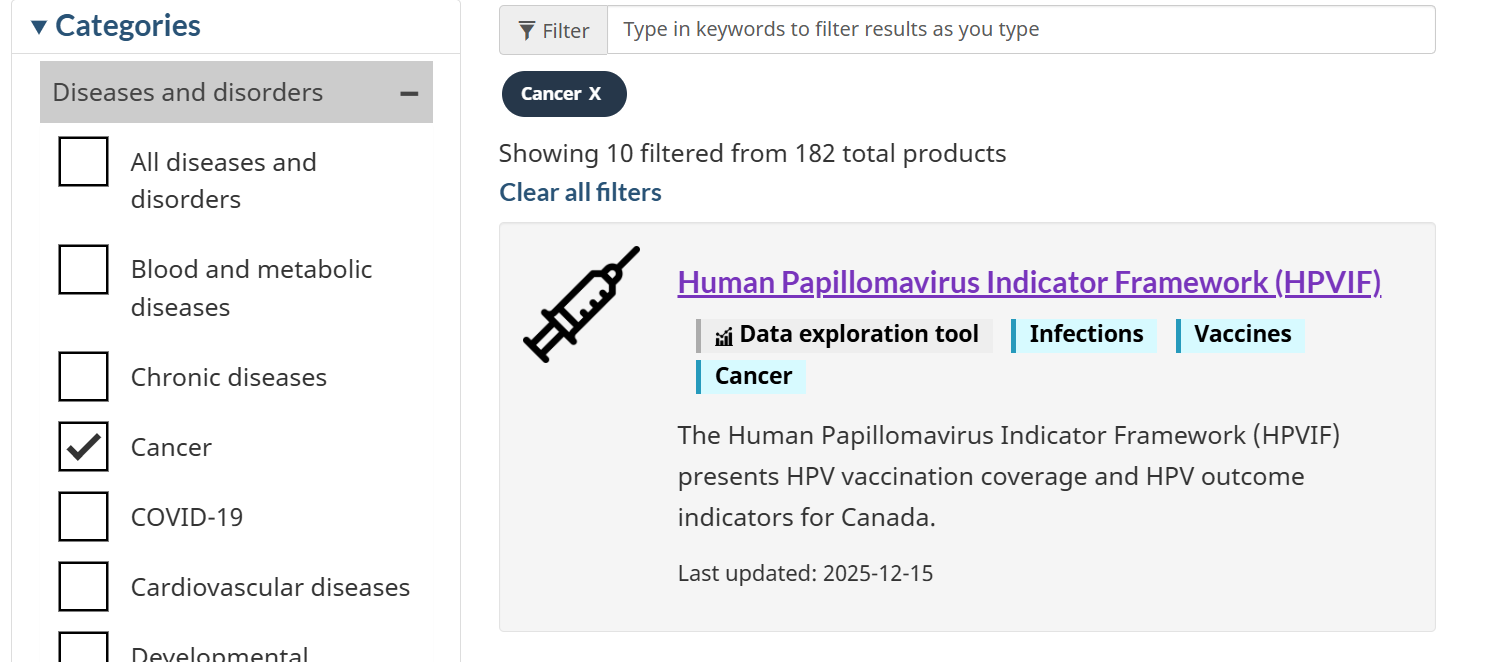
\includegraphics[width=0.9\linewidth,height=\textheight,keepaspectratio]{references/data-sources/../../assets/images/data8/infobase6.png}
\end{center}

\begin{center}
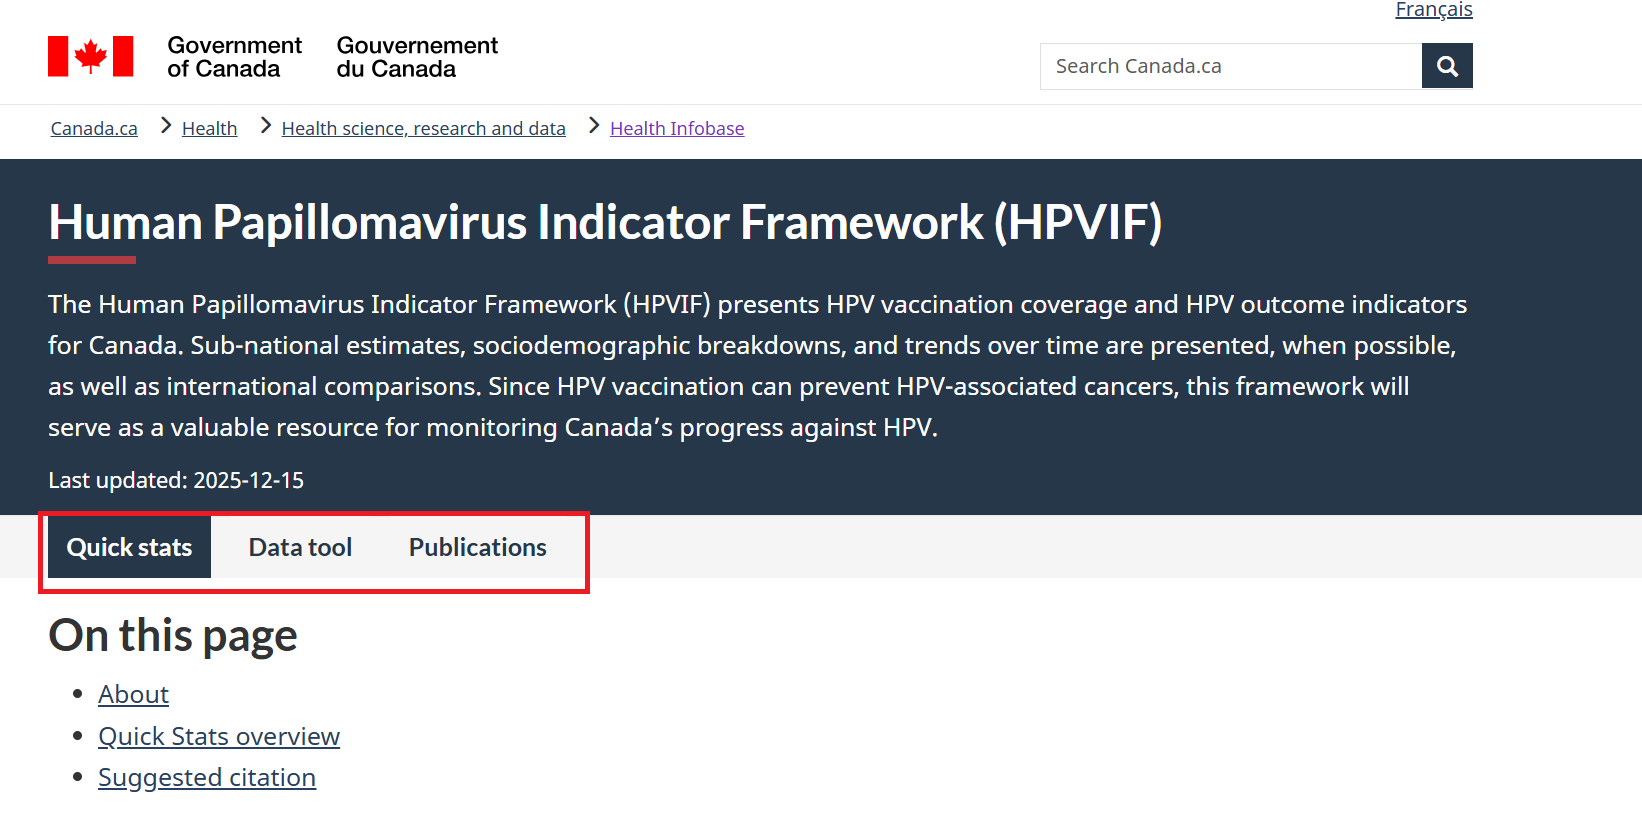
\includegraphics[width=0.9\linewidth,height=\textheight,keepaspectratio]{references/data-sources/../../assets/images/data8/infobase7.png}
\end{center}

The
\texttt{Drug\ and\ alcohol\ use\ in\ Canada:\ Postsecondary\ students}
product provides summary statistics as well as links to download data in
CSV format:

\begin{center}
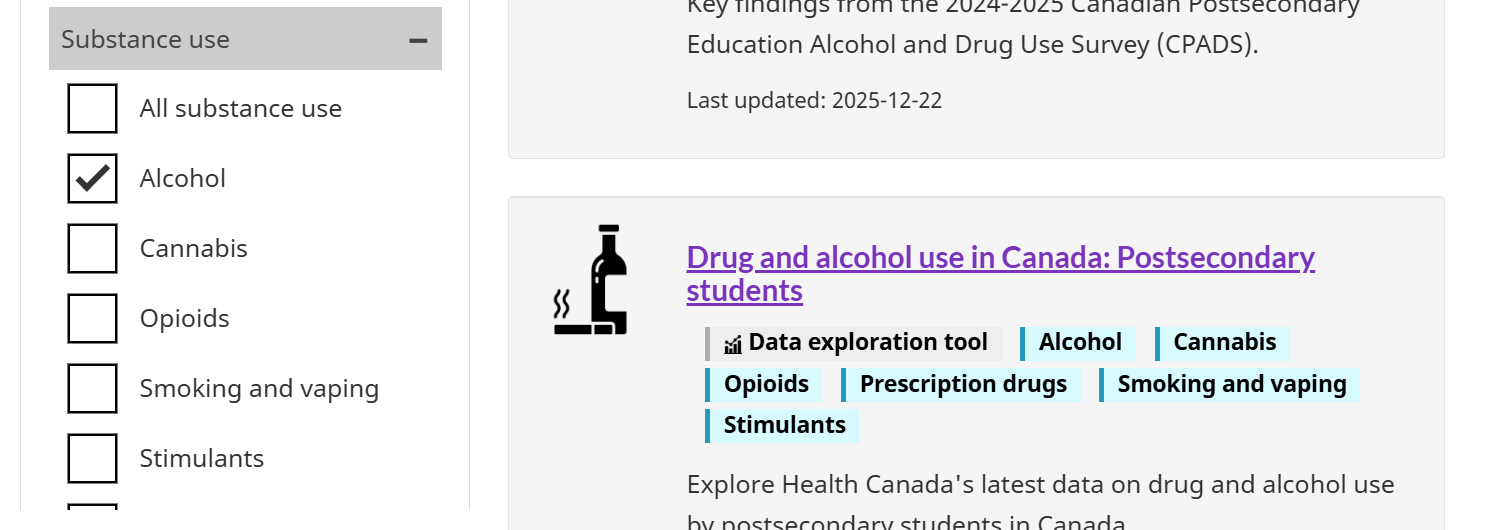
\includegraphics[width=0.9\linewidth,height=\textheight,keepaspectratio]{references/data-sources/../../assets/images/data8/infobase8.png}
\end{center}

\begin{center}

\includegraphics[width=0.9\linewidth,height=\textheight,keepaspectratio]{references/data-sources/../../assets/images/data8/infobase9.png}
\end{center}

\begin{center}
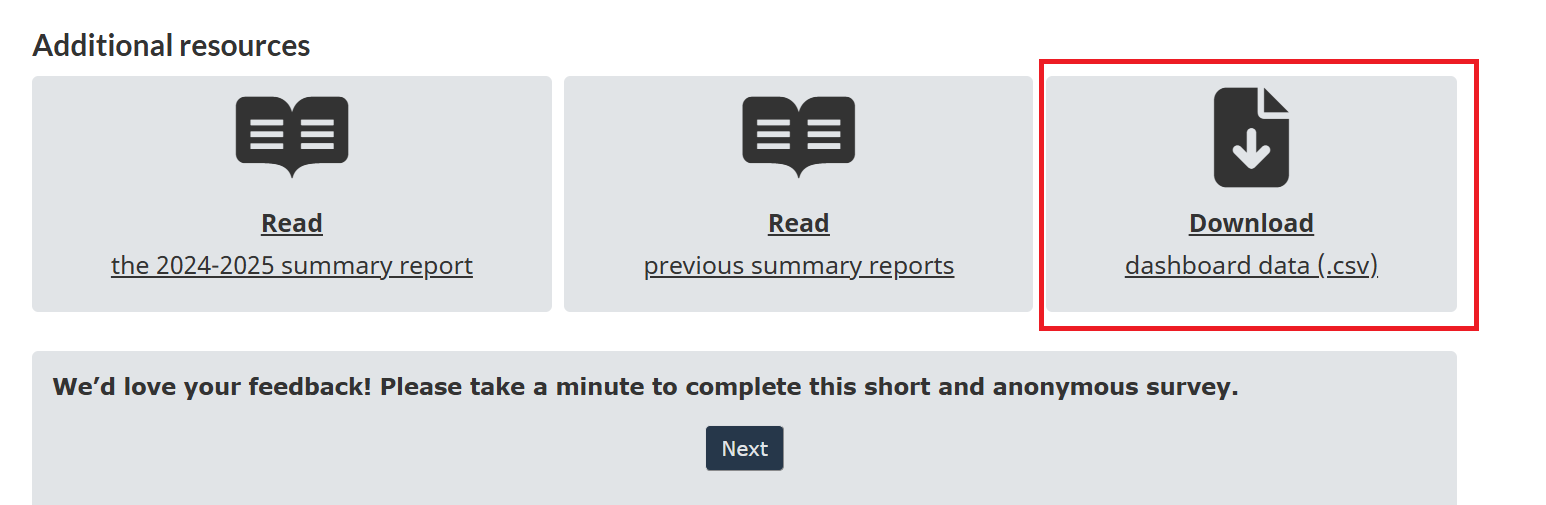
\includegraphics[width=0.9\linewidth,height=\textheight,keepaspectratio]{references/data-sources/../../assets/images/data8/infobase10.png}
\end{center}

\chapter*{CCDSS}\label{ccdss}
\addcontentsline{toc}{chapter}{CCDSS}

\markboth{CCDSS}{CCDSS}

The Canadian Chronic Disease Surveillance System (CCDSS) is a
collaborative network of provincial and territorial chronic disease
surveillance systems in Canada. The CCDSS is supported by the Public
Health Agency of Canada (PHAC) and provincial/territorial governments.
The CCDSS was established to provide the estimates of the prevalence and
incidence of chronic diseases in Canada, as well as to monitor trends
over time for more than 20 chronic diseases to help inform health
policies and resource planning. The CCDSS is part of the PHAC Health
Infobase that we covered in the previous tutorial on
\href{data8.html}{Health Infobase}. The CCDSS uses health administrative
data, such as hospital discharge records, physician billing claims, and
prescription drug data.

\begin{center}

\includegraphics[width=0.9\linewidth,height=\textheight,keepaspectratio]{references/data-sources/../../assets/images/data9/ccdss1.png}
\end{center}

\marginnote{\begin{footnotesize}

\href{https://health-infobase.canada.ca/ccdss/}{CCDSS website}

\end{footnotesize}}

\subsection*{Key Indicator Categories}\label{key-indicator-categories}
\addcontentsline{toc}{subsection}{Key Indicator Categories}

The CCDSS website provides a variety of indicators related to chronic
diseases, such as autism, cardiovascular diseases, chronic respiratory
diseases, diabetes, mental health disorders, musculoskeletal disorders,
neurological disorders, and multimorbidity.

\begin{center}
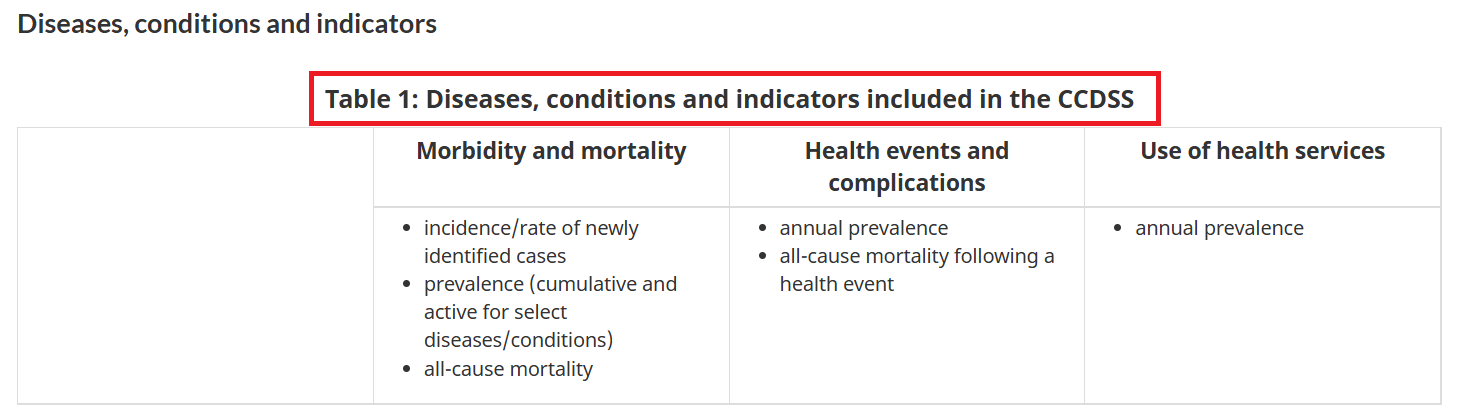
\includegraphics[width=0.9\linewidth,height=\textheight,keepaspectratio]{references/data-sources/../../assets/images/data9/ccdss2.png}
\end{center}

\begin{center}
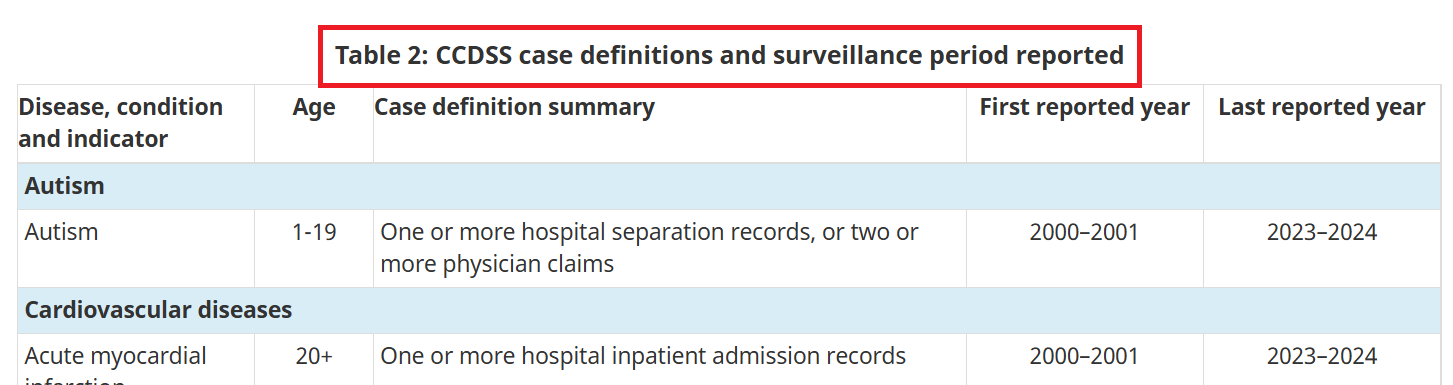
\includegraphics[width=0.9\linewidth,height=\textheight,keepaspectratio]{references/data-sources/../../assets/images/data9/ccdss3.png}
\end{center}

\subsection*{Data Tool}\label{data-tool}
\addcontentsline{toc}{subsection}{Data Tool}

The CCDSS website provides a data tool that allows users to explore and
visualize the data on chronic diseases in Canada. The data tool provides
interactive charts and tables that allow users to explore the data by
province/territory.

\begin{center}

\includegraphics[width=0.9\linewidth,height=\textheight,keepaspectratio]{references/data-sources/../../assets/images/data9/ccdss4.png}
\end{center}

\marginnote{\begin{footnotesize}

\href{https://health-infobase.canada.ca/ccdss/data-tool/Index}{CCDSS
Data Tool}

\end{footnotesize}}

Users can use the data tool to explore the prevalence and incidence of
cases, mortality rates, and health service utilization, and to track
individuals living with two or more chronic conditions.

\begin{center}
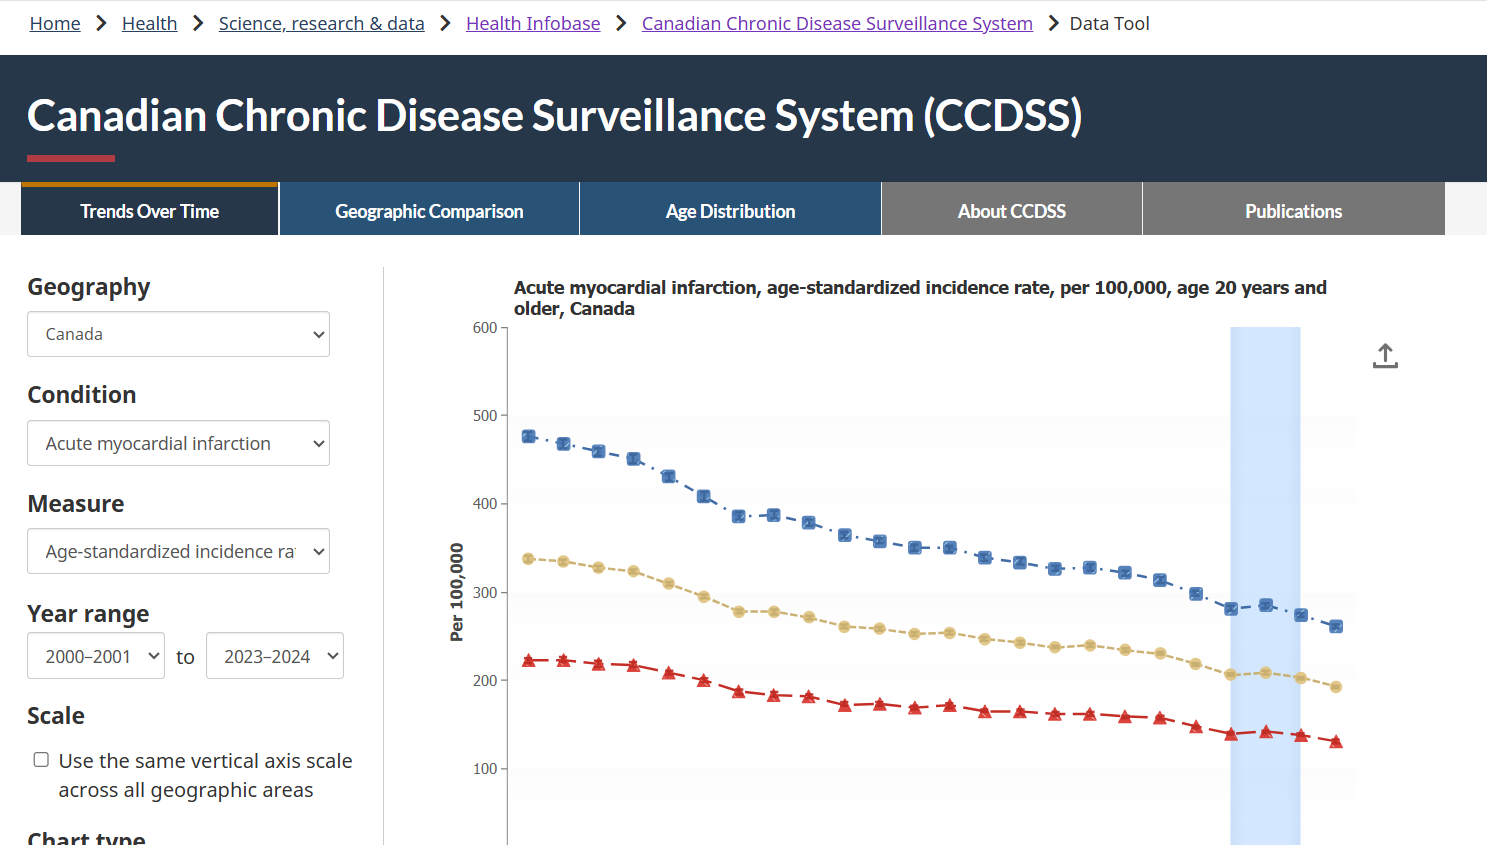
\includegraphics[width=0.9\linewidth,height=\textheight,keepaspectratio]{references/data-sources/../../assets/images/data9/ccdss5.png}
\end{center}

Users can explore trends over time, compare data across
provinces/territories, and view the distribution of cases by age group.
Under the \texttt{Publication} tab, you can find information on the
repository for data-driven insights, fact sheets, peer-reviewed
publications, and reports.

\begin{center}
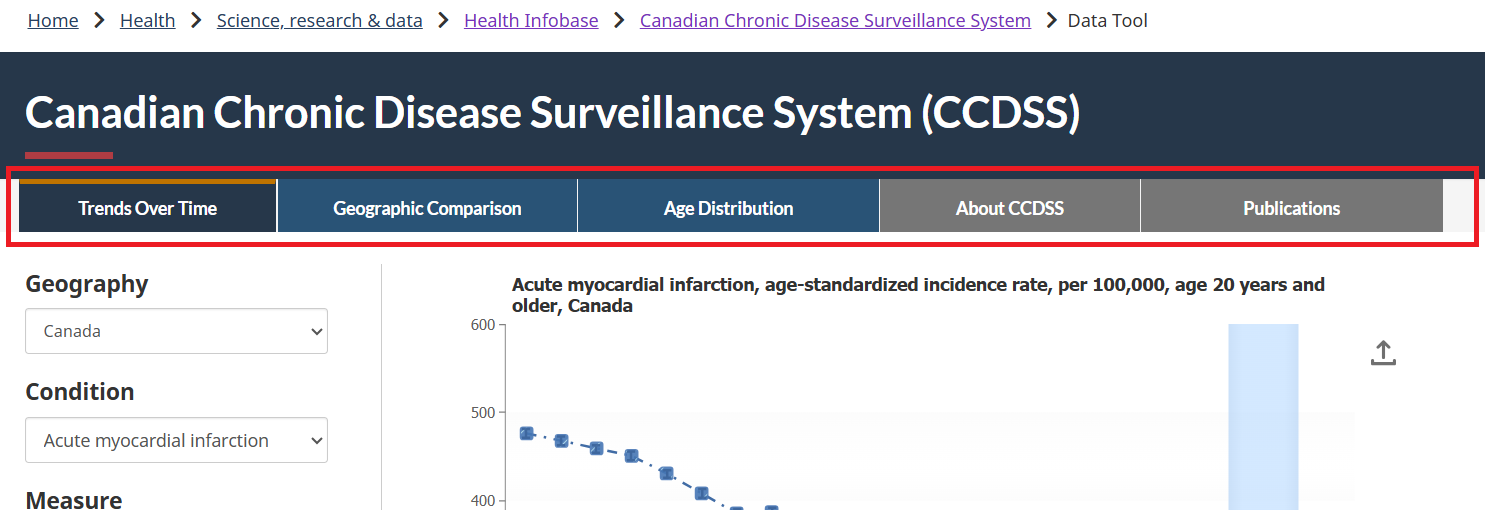
\includegraphics[width=0.9\linewidth,height=\textheight,keepaspectratio]{references/data-sources/../../assets/images/data9/ccdss6.png}
\end{center}

\subsection*{Interactive chart example}\label{interactive-chart-example}
\addcontentsline{toc}{subsection}{Interactive chart example}

Consider \texttt{Asthma} under \texttt{Chronic\ respiratory\ diseases}
as an example.

\begin{center}
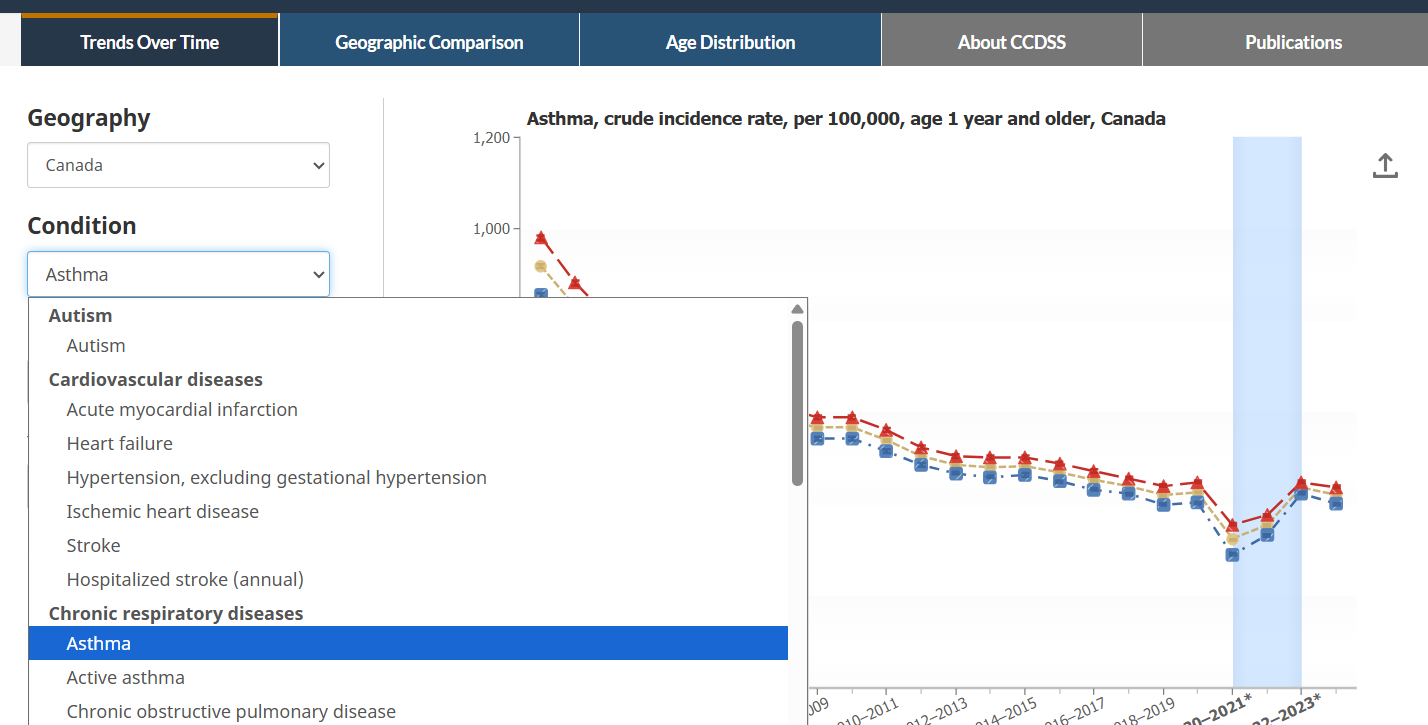
\includegraphics[width=0.9\linewidth,height=\textheight,keepaspectratio]{references/data-sources/../../assets/images/data9/ccdss7.png}
\end{center}

You can explore different summary measures by filtering by geography,
measure, and year. Again, you can further explore trends over time,
compare data across provinces/territories, and view the distribution of
cases by age group.

\begin{center}
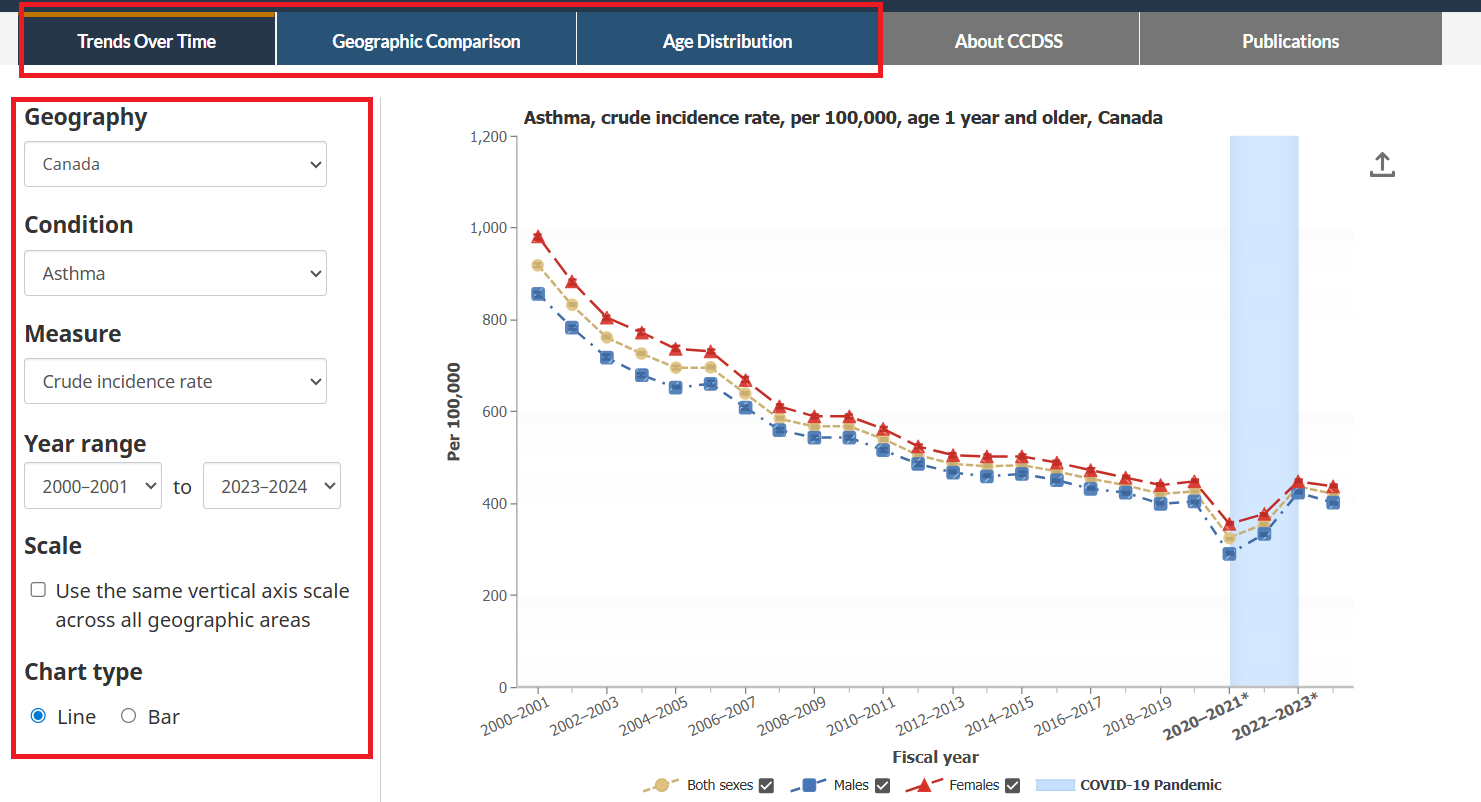
\includegraphics[width=0.9\linewidth,height=\textheight,keepaspectratio]{references/data-sources/../../assets/images/data9/ccdss8.png}
\end{center}

You can also download the summary data in CSV format for further
analysis. To do that, you need to scroll down to the bottom of the
\texttt{Summary\ Table}, and click on the \texttt{Download} button.

\begin{center}
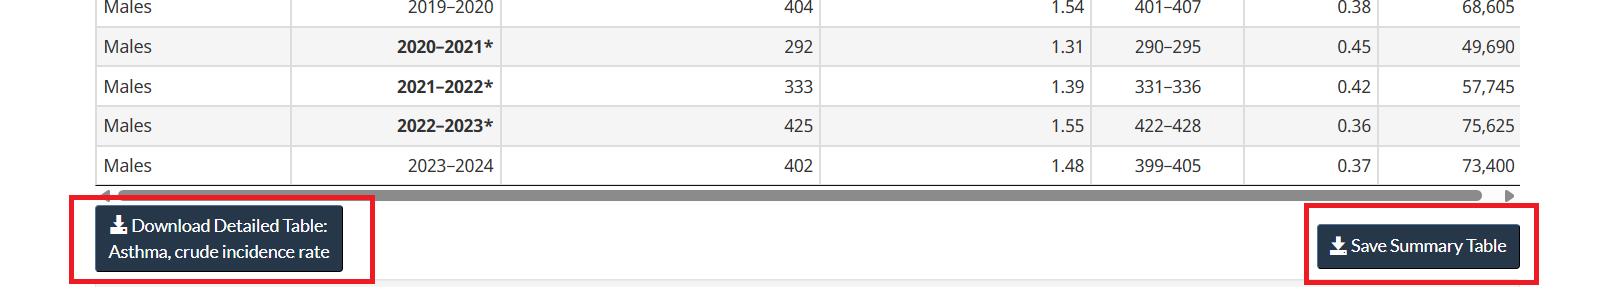
\includegraphics[width=0.9\linewidth,height=\textheight,keepaspectratio]{references/data-sources/../../assets/images/data9/ccdss9.png}
\end{center}

Once you open the CSV file in Excel or other software, you will find
that the data is not at the individual or person level. Instead, the
data are aggregated at the country and province/territory levels, and
summary measures are provided for both sexes and for years. For example,
see row 4. The \texttt{Geography} column says \emph{Canada} and the
\texttt{Rate\ (per\ 100,000)} column says \emph{919}. This is an example
of aggregate data.

\begin{center}
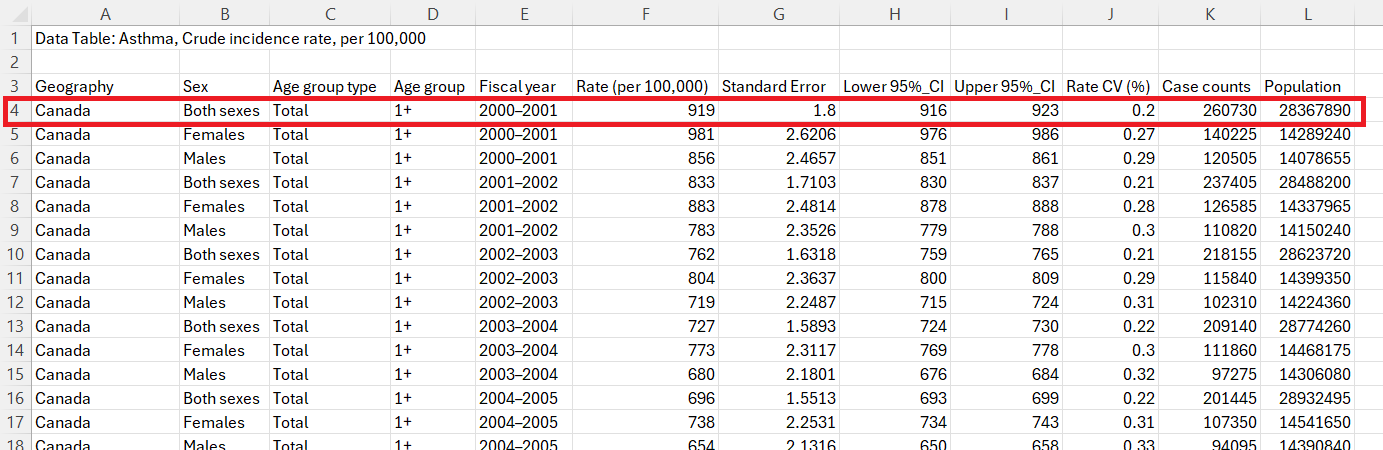
\includegraphics[width=0.9\linewidth,height=\textheight,keepaspectratio]{references/data-sources/../../assets/images/data9/ccdss10.png}
\end{center}

Because this data is not at the person-level, and the summary measures
are aggregated, you do not need a codebook to translate columns.
However, you cannot use this data to calculate the prevalence or
incidence of asthma in Canada because it is already aggregated. You can
only use this data to explore the trends over time, compare data across
provinces/territories, and view the distribution of cases by age group
and sex. The individual patients have already been erased to protect
their privacy.

\chapter*{GHO}\label{gho}
\addcontentsline{toc}{chapter}{GHO}

\markboth{GHO}{GHO}

The Global Health Observatory (GHO) is the World Health Organization's
(WHO) main health statistics repository. The GHO provides data on a wide
range of health topics, such as mortality, morbidity, risk factors,
health systems, and health equity. The GHO collects data from member
states, international organizations, and other sources to provide a
comprehensive picture of global health. The GHO is a valuable resource
for researchers, policymakers, and public health professionals who are
interested in understanding global health trends and disparities. The
GHO provides various ways to interact with its data, including
interactive maps and downloadable CSV files.

\begin{center}
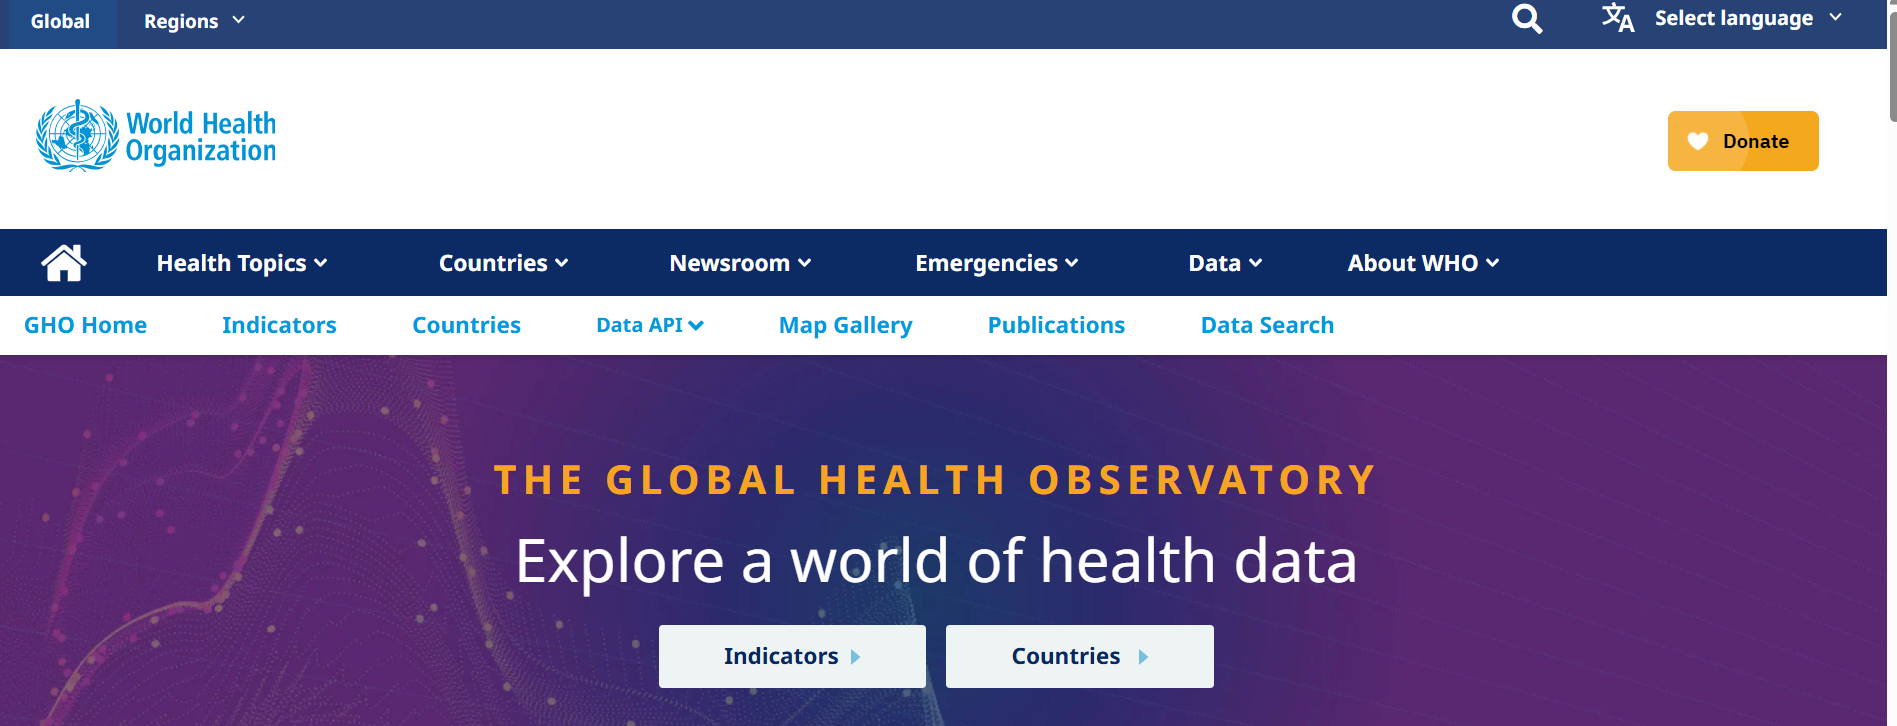
\includegraphics[width=0.9\linewidth,height=\textheight,keepaspectratio]{references/data-sources/../../assets/images/data10/gho1.png}
\end{center}

\marginnote{\begin{footnotesize}

\href{https://www.who.int/data/gho}{WHO Global Health Observatory}

\end{footnotesize}}

\subsection*{World Health Data}\label{world-health-data}
\addcontentsline{toc}{subsection}{World Health Data}

You can browse information by broader health indicators or by specific
countries.

\begin{center}

\includegraphics[width=0.9\linewidth,height=\textheight,keepaspectratio]{references/data-sources/../../assets/images/data10/gho2.png}
\end{center}

To explore the data by indicators, click on the \texttt{Indicators} tab.
You can find a list of indicators across categories such as
\texttt{Hepatitis}, \texttt{Nutrition}, \texttt{Mental\ health}, and so
on.

\begin{center}

\includegraphics[width=0.9\linewidth,height=\textheight,keepaspectratio]{references/data-sources/../../assets/images/data10/gho3.png}
\end{center}

\begin{center}
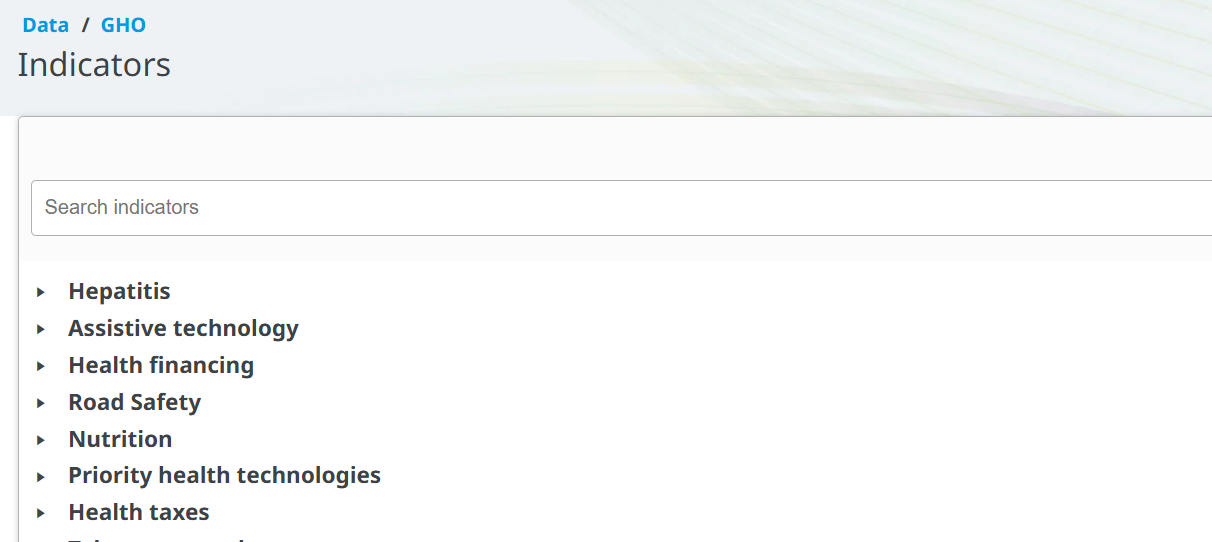
\includegraphics[width=0.9\linewidth,height=\textheight,keepaspectratio]{references/data-sources/../../assets/images/data10/gho4.png}
\end{center}

You can also use the search bar to search for specific indicators. For
example, if you search for \texttt{Life\ expectancy\ at\ birth}, you
will find a list of indicators related to life expectancy, such as
\texttt{Life\ expectancy\ at\ birth\ (years)}.

\begin{center}
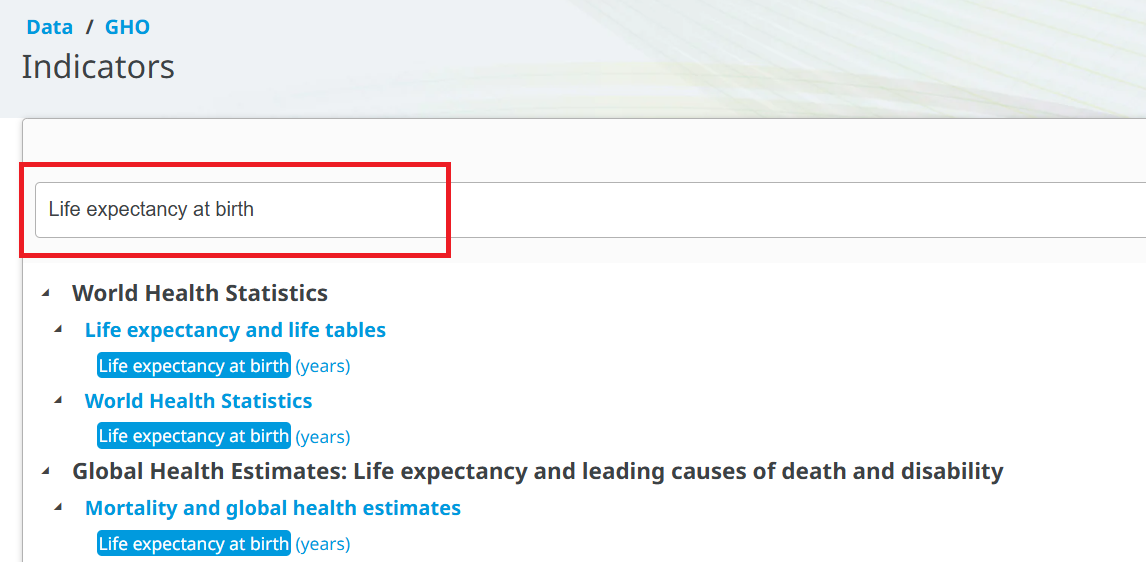
\includegraphics[width=0.9\linewidth,height=\textheight,keepaspectratio]{references/data-sources/../../assets/images/data10/gho5.png}
\end{center}

To explore the data by country, click on the \texttt{Countries} tab. You
can find a list of countries and regions. You can click the country name
to see the data for that country.

\begin{center}
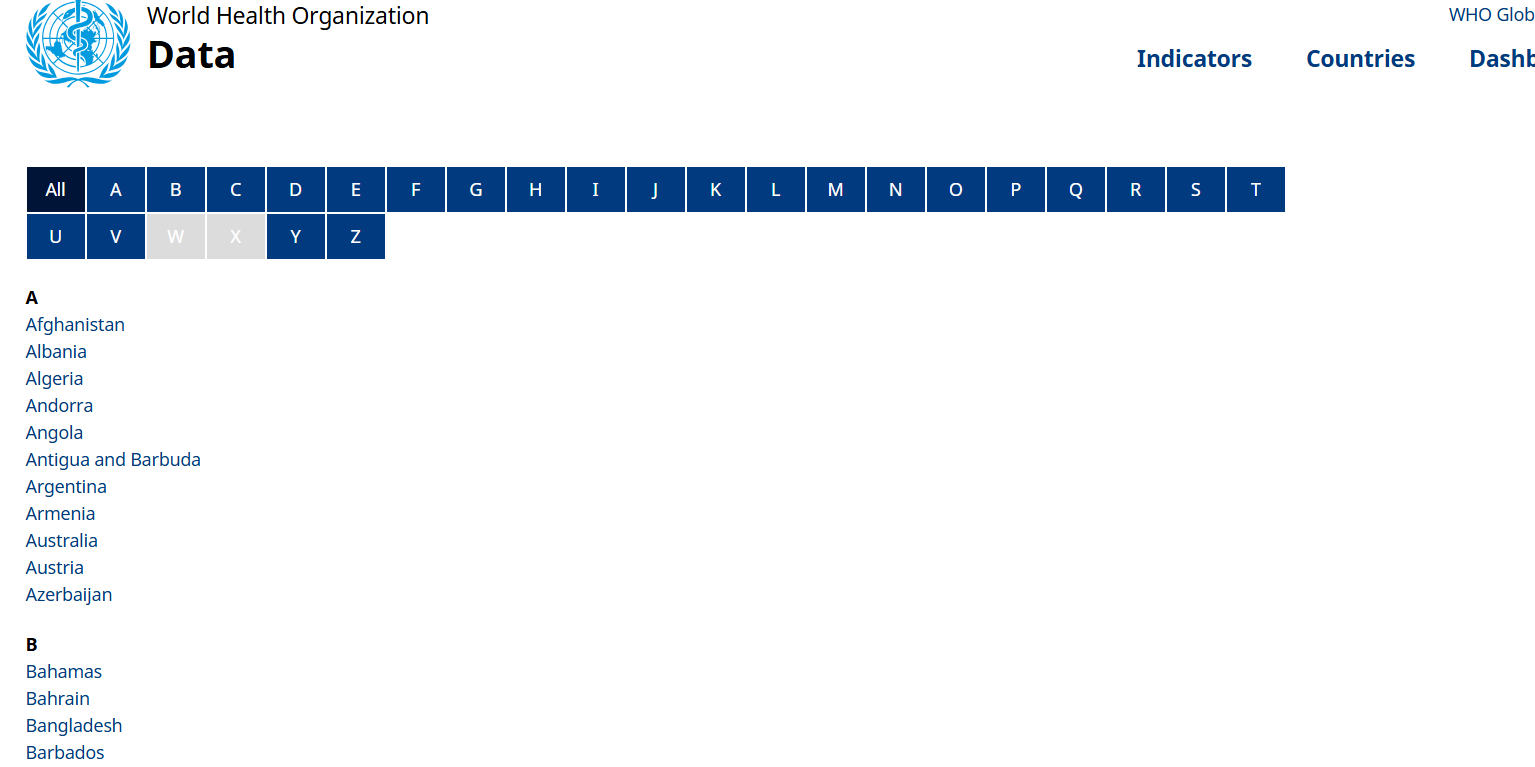
\includegraphics[width=0.9\linewidth,height=\textheight,keepaspectratio]{references/data-sources/../../assets/images/data10/gho6.png}
\end{center}

\begin{center}
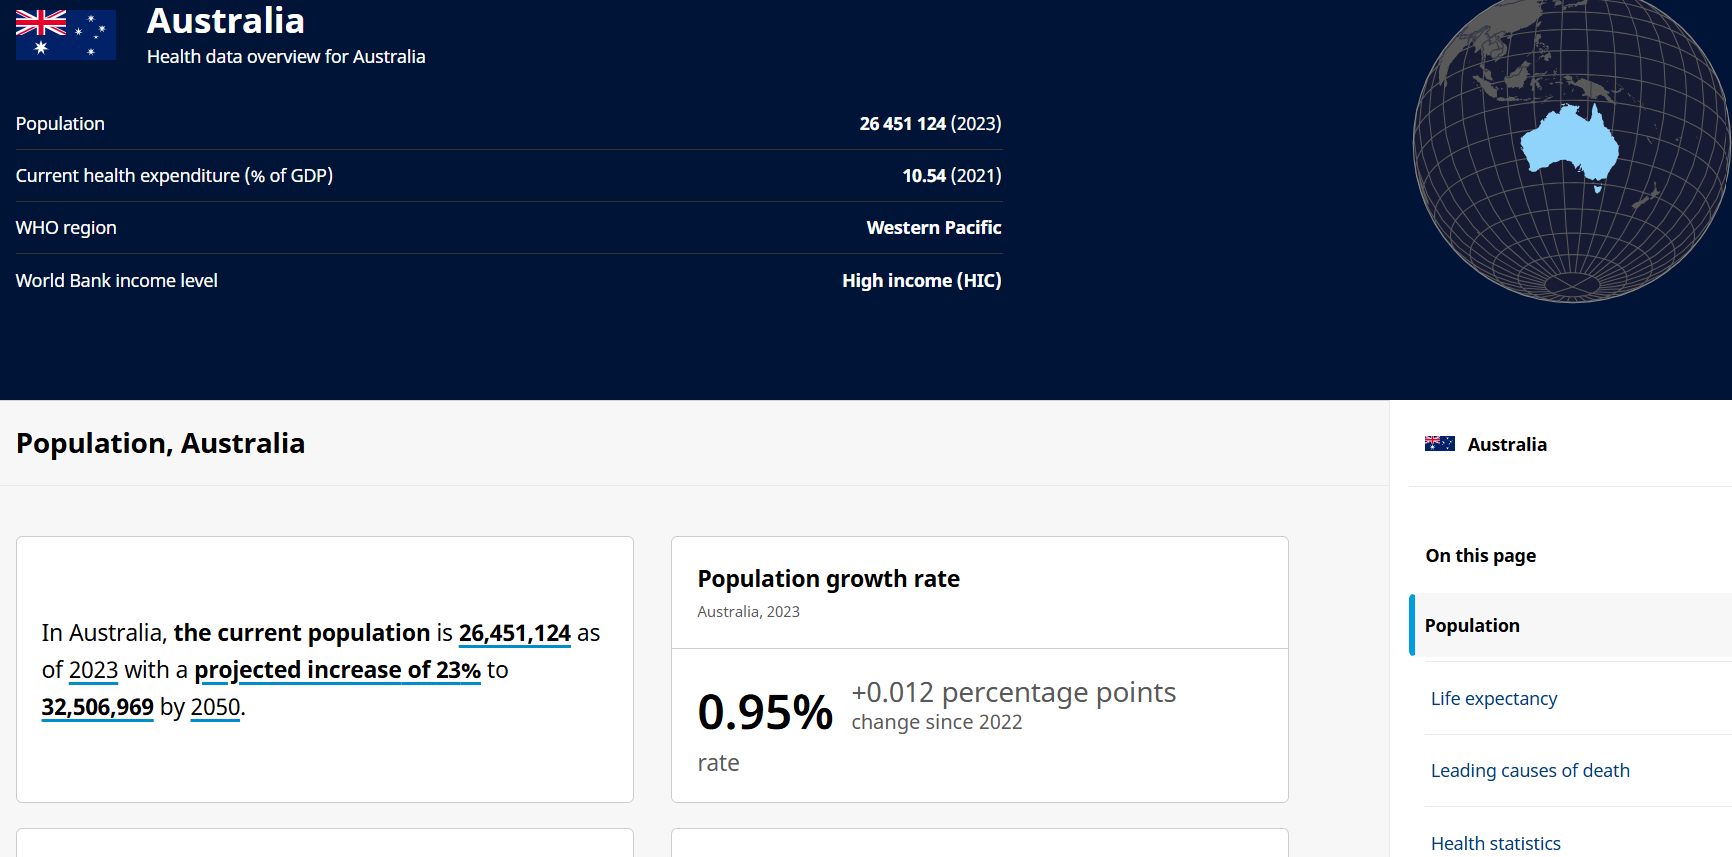
\includegraphics[width=0.9\linewidth,height=\textheight,keepaspectratio]{references/data-sources/../../assets/images/data10/gho7.png}
\end{center}

\subsection*{Data by indicator example}\label{data-by-indicator-example}
\addcontentsline{toc}{subsection}{Data by indicator example}

Let's click on the \texttt{Life\ expectancy\ at\ birth\ (years)}
indicator to see the details:

\begin{center}
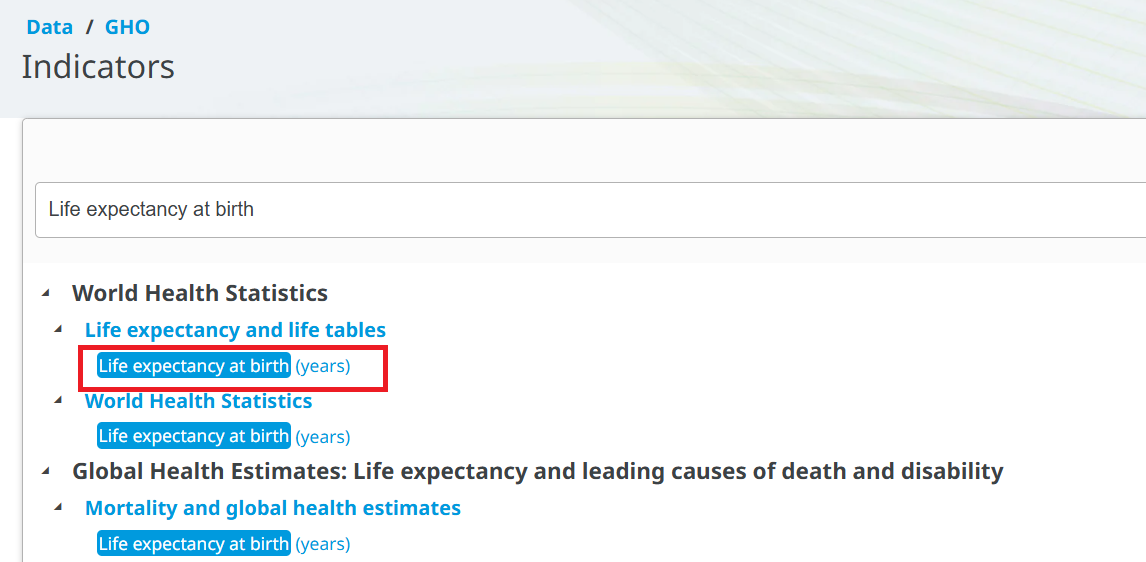
\includegraphics[width=0.9\linewidth,height=\textheight,keepaspectratio]{references/data-sources/../../assets/images/data10/gho8.png}
\end{center}

\marginnote{\begin{footnotesize}

\href{https://www.who.int/data/gho/data/indicators}{GHO Indicators}

\end{footnotesize}}

You can find different visualization options, such as charts and maps.
You can also download the chart and map to your computer.

\begin{center}
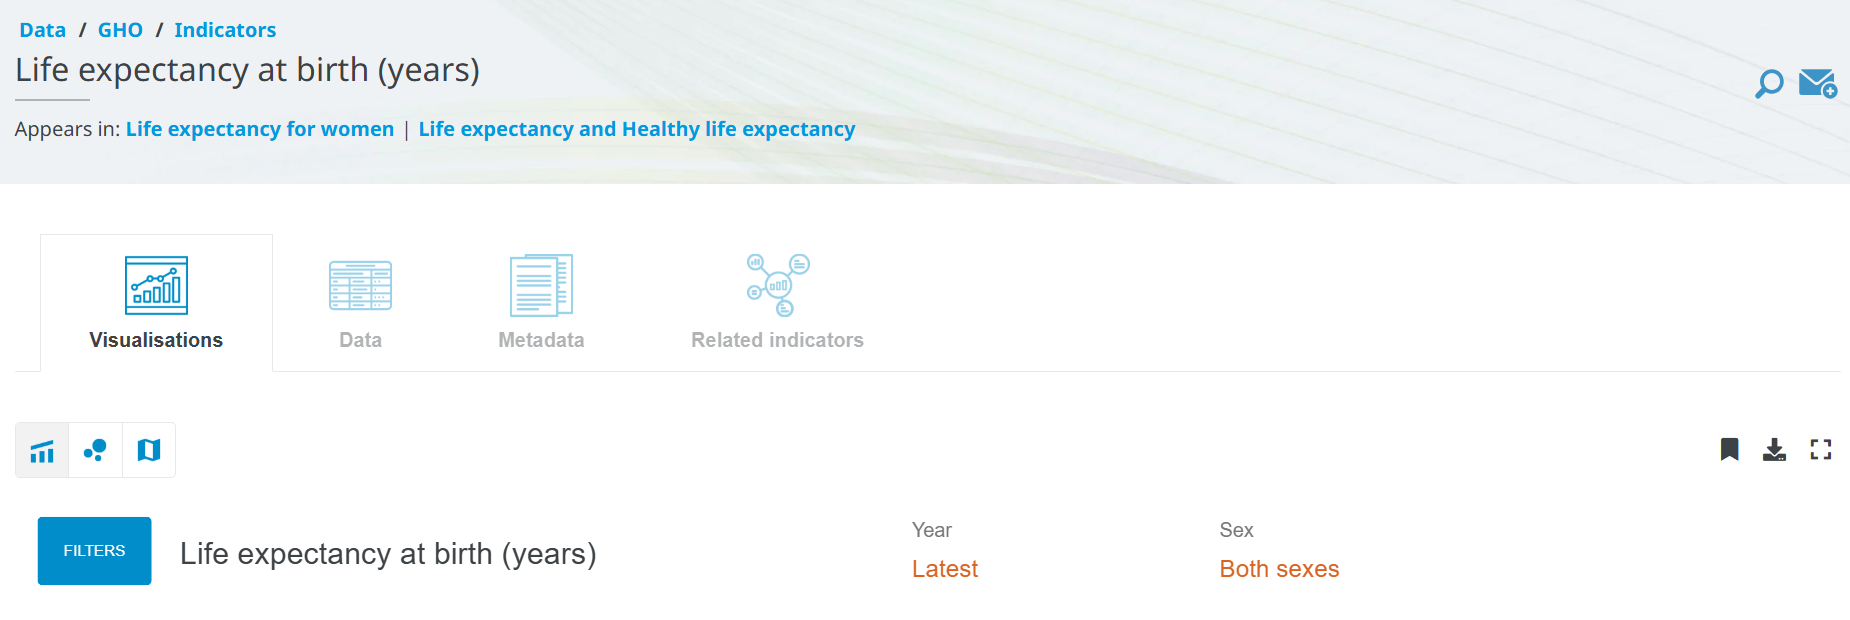
\includegraphics[width=1\linewidth,height=\textheight,keepaspectratio]{references/data-sources/../../assets/images/data10/gho9.png}
\end{center}

\begin{center}
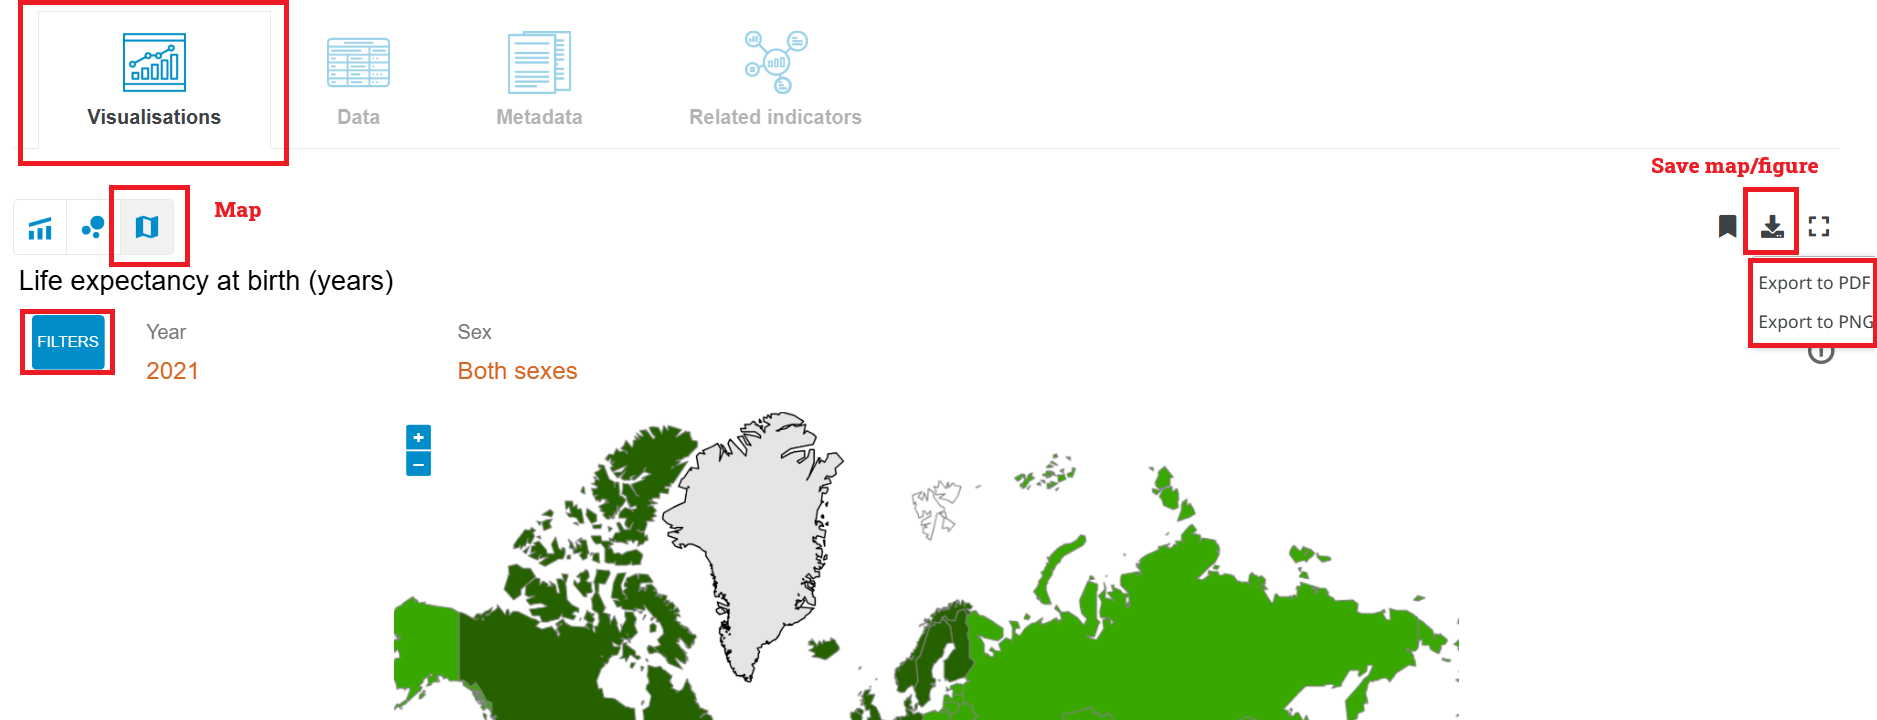
\includegraphics[width=1\linewidth,height=\textheight,keepaspectratio]{references/data-sources/../../assets/images/data10/gho10.png}
\end{center}

To see the data table, you can check the \texttt{Data} section. You can
also download the data in CSV format for further analysis. To do that,
you need to click on the \texttt{Download} button at the top right
corner of the data table.

\begin{center}
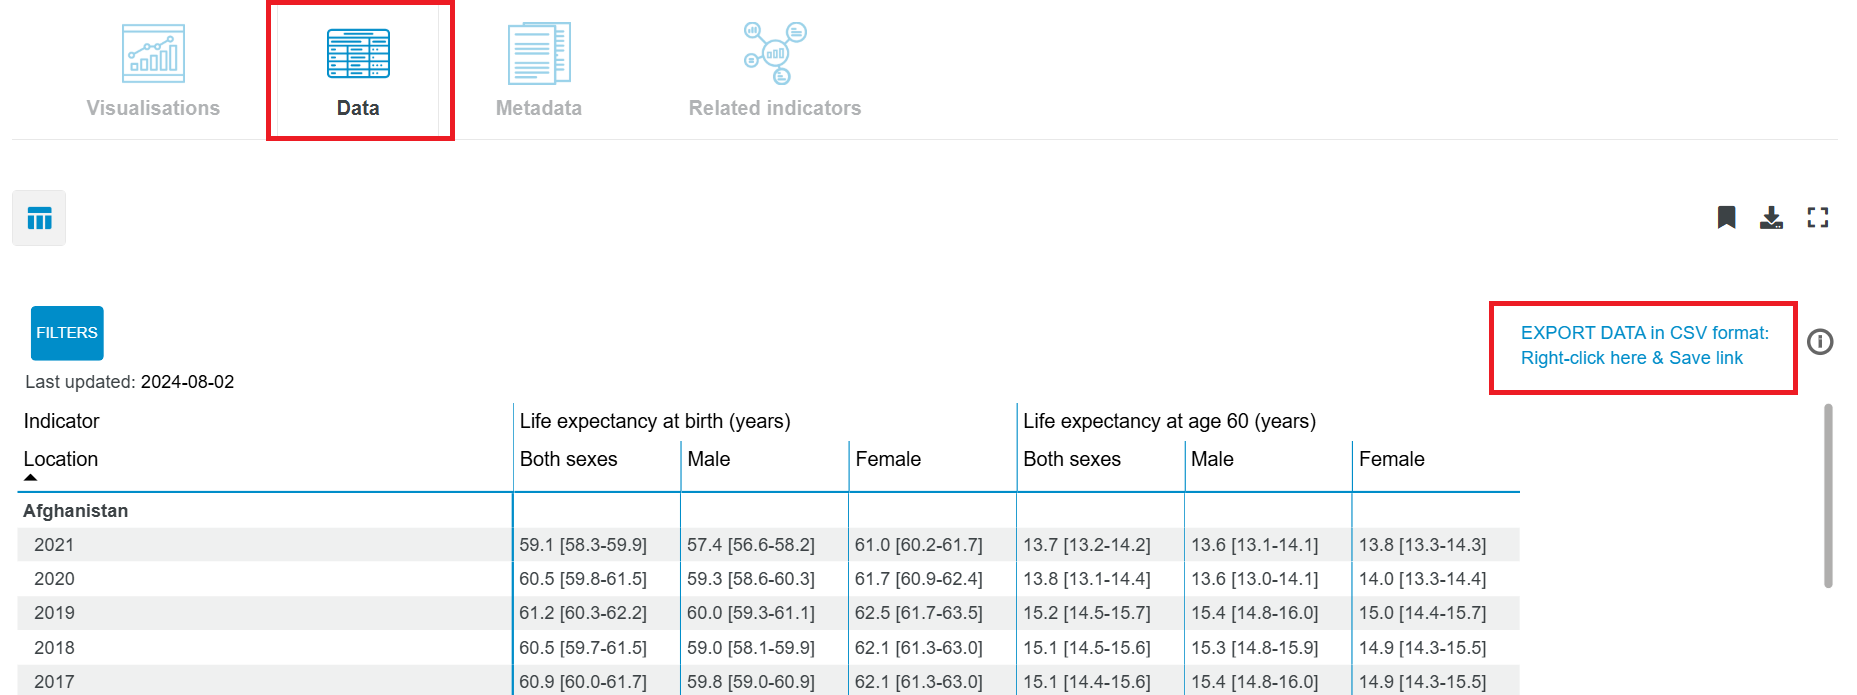
\includegraphics[width=1\linewidth,height=\textheight,keepaspectratio]{references/data-sources/../../assets/images/data10/gho11.png}
\end{center}

Similar to the \href{data9.html}{Canadian Chronic Disease Surveillance
System (CCDSS) database}, the life expectancy data is also at an
aggregated level, which means that the data is summarized at the country
level, and does not contain individual-level data:

\begin{center}
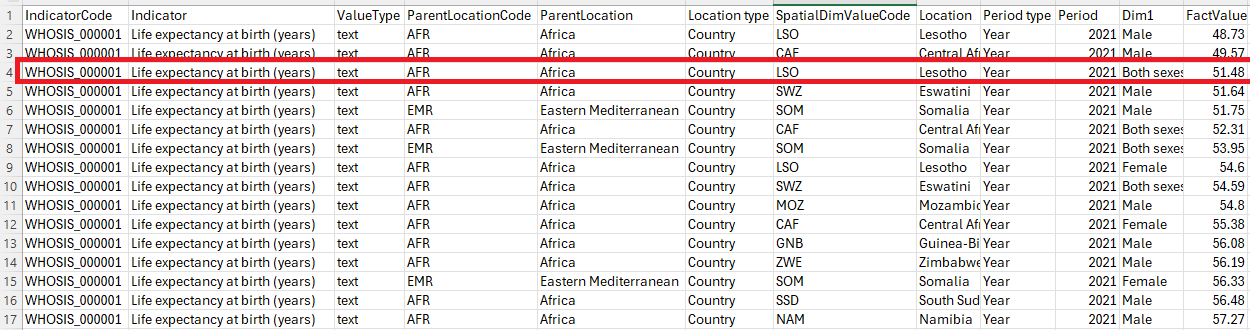
\includegraphics[width=1\linewidth,height=\textheight,keepaspectratio]{references/data-sources/../../assets/images/data10/gho12.png}
\end{center}

The data on the website, as well as the downloaded data in CSV format,
both provide the point estimate with 95\% confidence interval:

\begin{center}
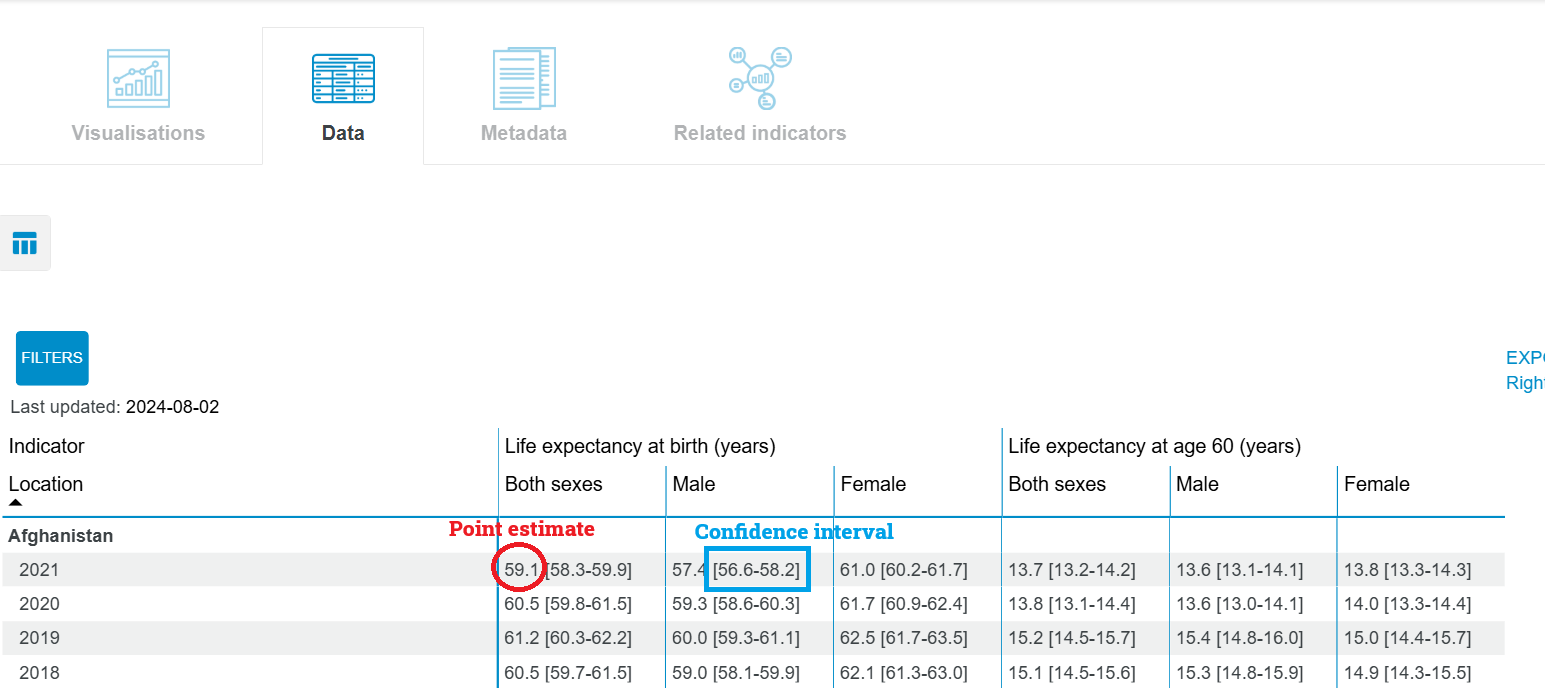
\includegraphics[width=1\linewidth,height=\textheight,keepaspectratio]{references/data-sources/../../assets/images/data10/gho13.png}
\end{center}

\subsection*{Data by country example}\label{data-by-country-example}
\addcontentsline{toc}{subsection}{Data by country example}

Let's click on \texttt{Canada} to explore the data for Canada.

\begin{center}
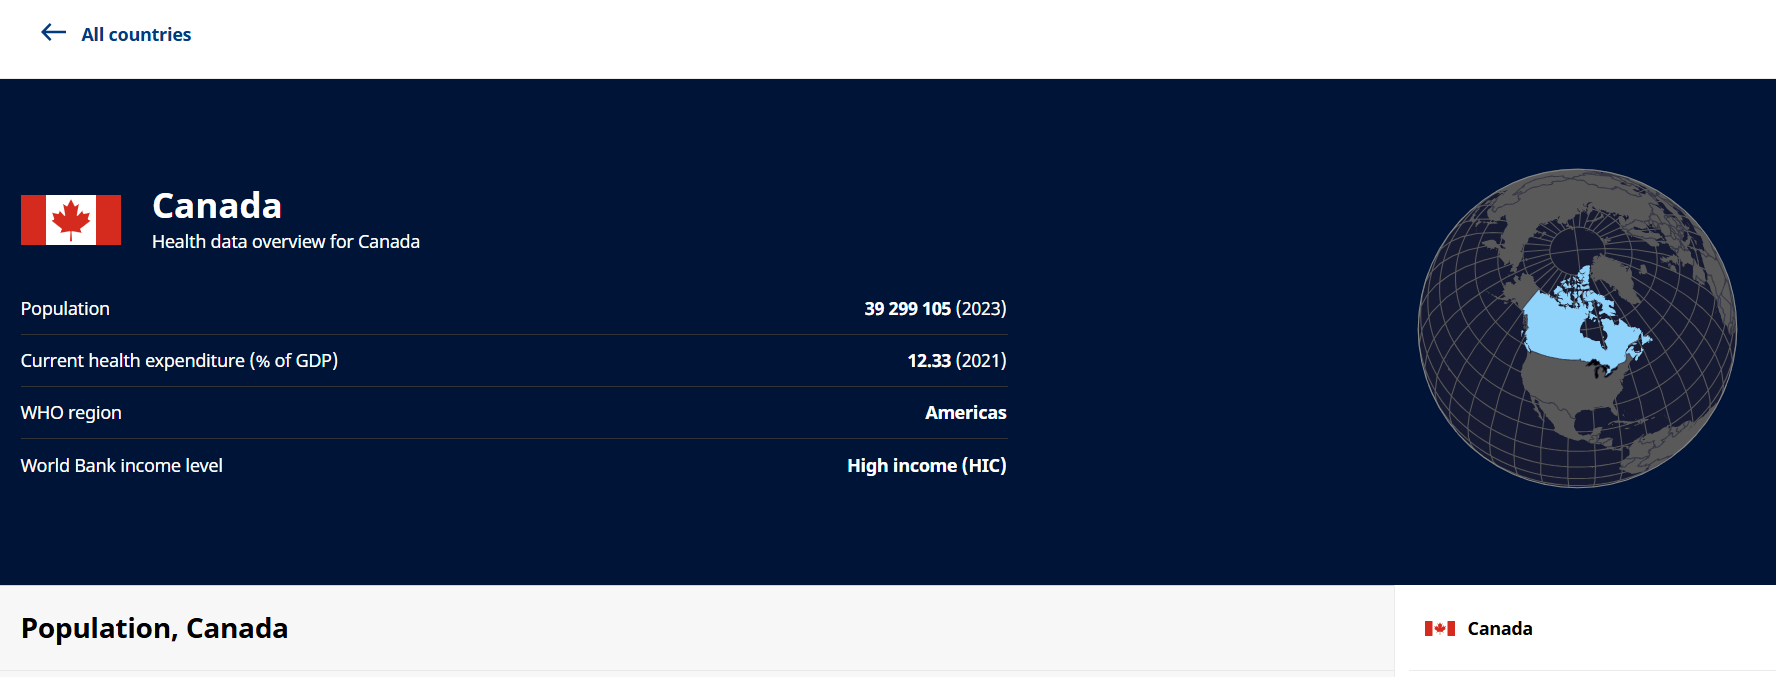
\includegraphics[width=0.9\linewidth,height=\textheight,keepaspectratio]{references/data-sources/../../assets/images/data10/gho14.png}
\end{center}

\marginnote{\begin{footnotesize}

\href{https://data.who.int/countries}{GHO Data by Country}

\end{footnotesize}}

You can explore different indicators for Canada. You can also download
all indicators as a ZIP file by clicking \texttt{Reference\ data}.

\begin{center}
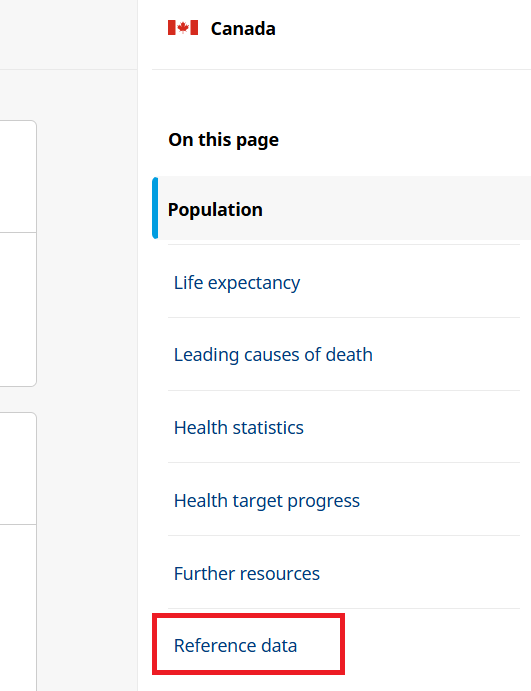
\includegraphics[width=0.75\linewidth,height=\textheight,keepaspectratio]{references/data-sources/../../assets/images/data10/gho15.png}
\end{center}

\begin{center}

\includegraphics[width=0.6\linewidth,height=\textheight,keepaspectratio]{references/data-sources/../../assets/images/data10/gho16.png}
\end{center}

Once you unzip the folder, you will find several folders. Each folder
contains a codelist, data, a data dictionary, along with a license and
terms of use for different indicators.

\begin{center}
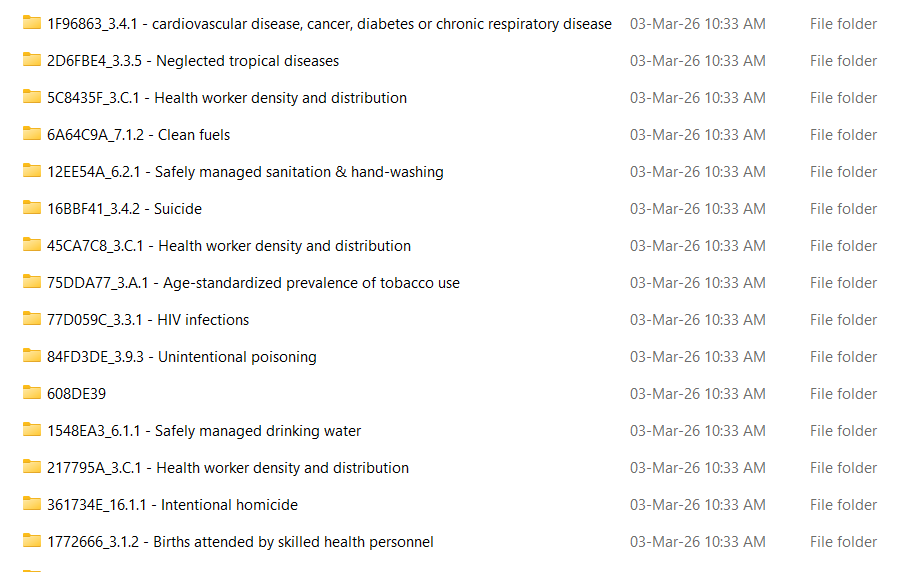
\includegraphics[width=0.9\linewidth,height=\textheight,keepaspectratio]{references/data-sources/../../assets/images/data10/gho17.png}
\end{center}

For example, the \texttt{77D059C\_3.3.1\ -\ HIV\ infections} folder
contains the following files:

\begin{center}
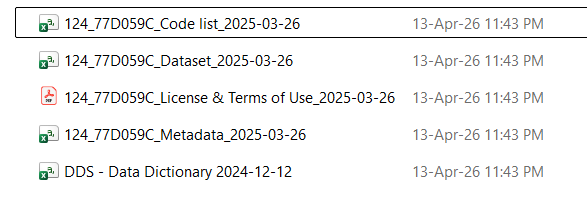
\includegraphics[width=0.9\linewidth,height=\textheight,keepaspectratio]{references/data-sources/../../assets/images/data10/gho18.png}
\end{center}

\subsection*{Metadata}\label{metadata}
\addcontentsline{toc}{subsection}{Metadata}

The GHO provides metadata for each indicator, providing important
context for understanding the data and its limitations. For example, the
metadata for the \texttt{Hepatitis\ -\ new\ infections} indicator
includes information on the definition of the indicator, the methods
used to calculate the indicator, data sources, and other relevant
information.

\marginnote{\begin{footnotesize}

\href{https://www.who.int/data/gho/indicator-metadata-registry}{Indicator
Metadata Registry List}

\end{footnotesize}}

\begin{center}
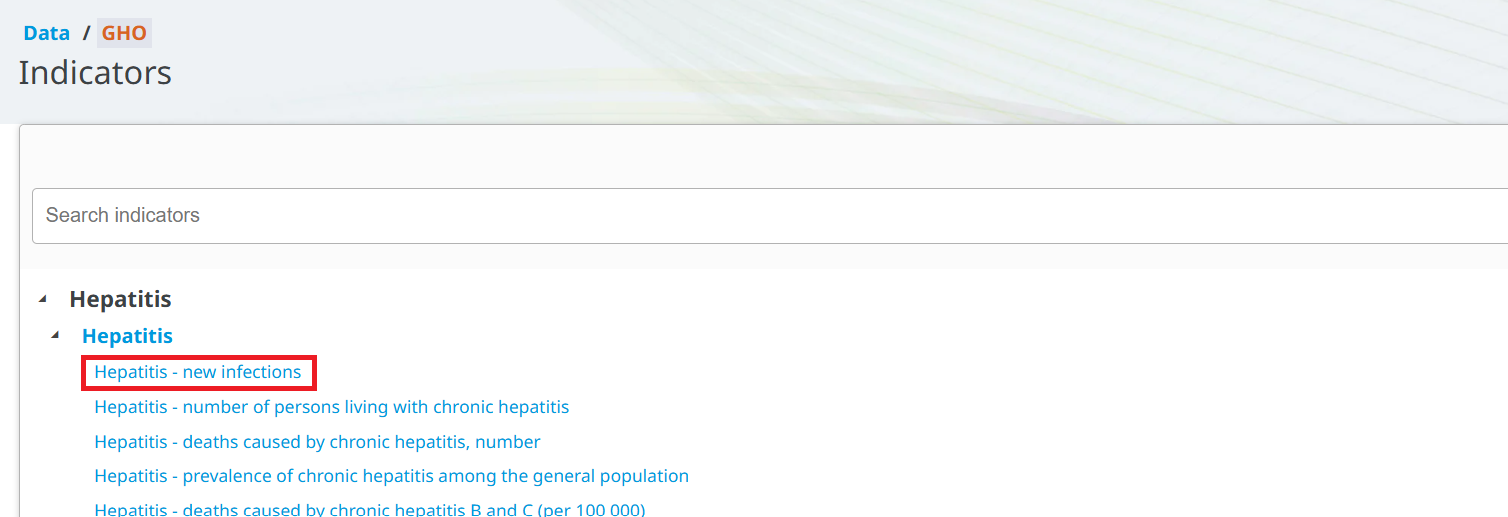
\includegraphics[width=1\linewidth,height=\textheight,keepaspectratio]{references/data-sources/../../assets/images/data10/gho19.png}
\end{center}

\begin{center}
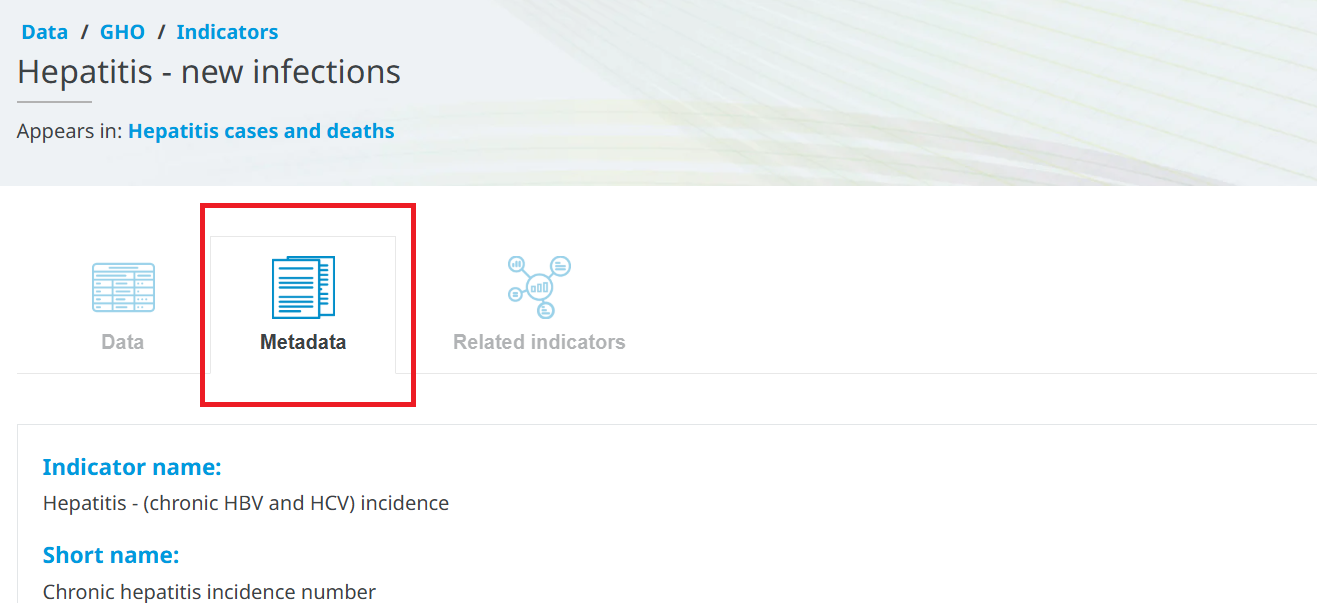
\includegraphics[width=1\linewidth,height=\textheight,keepaspectratio]{references/data-sources/../../assets/images/data10/gho20.png}
\end{center}

\chapter*{Open Portal}\label{open-portal}
\addcontentsline{toc}{chapter}{Open Portal}

\markboth{Open Portal}{Open Portal}

Open Government Portal Canada is a platform that provides access to
searching for a wide range of public data. Users can explore and
download data in different formats under the
\href{https://open.canada.ca/en/open-government-licence-canada}{Open
Government Licence - Canada}.

\begin{center}

\includegraphics[width=0.9\linewidth,height=\textheight,keepaspectratio]{references/data-sources/../../assets/images/data11/open1.png}
\end{center}

\marginnote{\begin{footnotesize}

\href{https://open.canada.ca/en}{Open Government Portal Canada}

\end{footnotesize}}

\subsection*{Search for Open Data}\label{search-for-open-data}
\addcontentsline{toc}{subsection}{Search for Open Data}

To search for open data, you can use the search bar on the Open
Government Portal Canada homepage. For example, if you are interested in
finding data on ``hospital locations'', you can enter that term in the
search bar and click the search icon. There are many filter options to
narrow your search results, such as format and organization.

\begin{center}
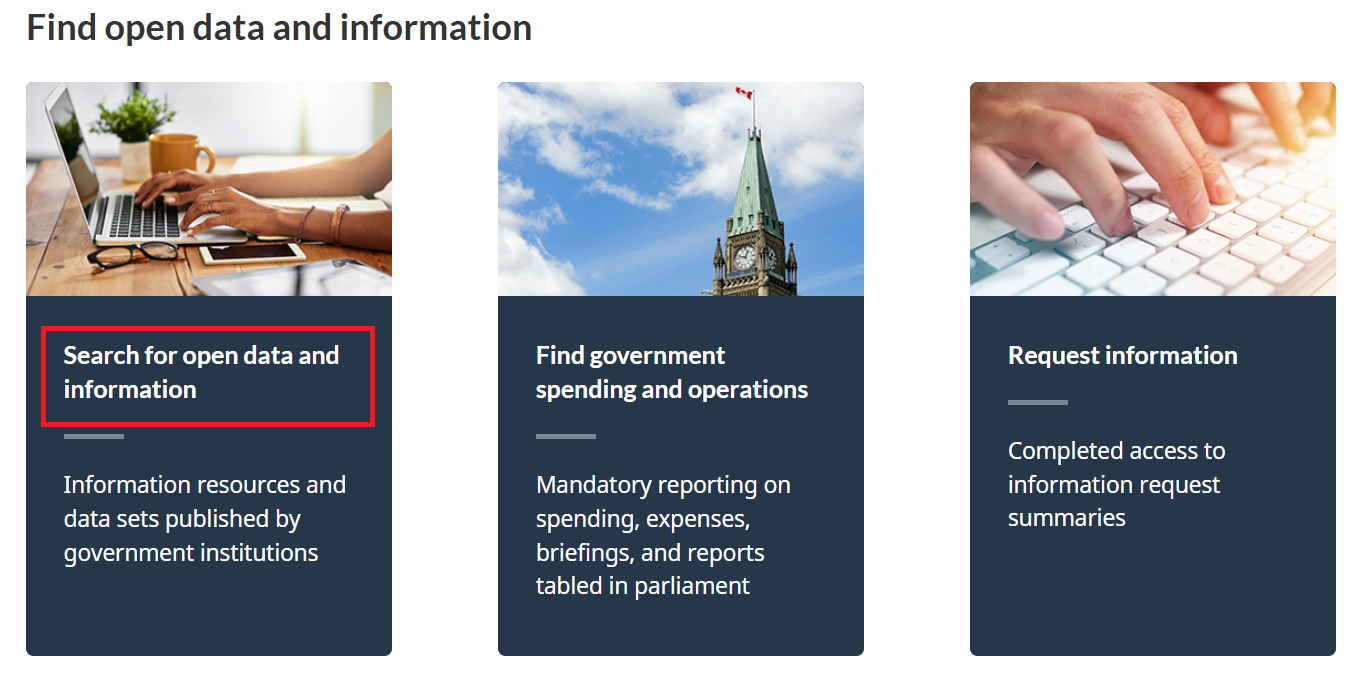
\includegraphics[width=0.9\linewidth,height=\textheight,keepaspectratio]{references/data-sources/../../assets/images/data11/open2.png}
\end{center}

\begin{center}
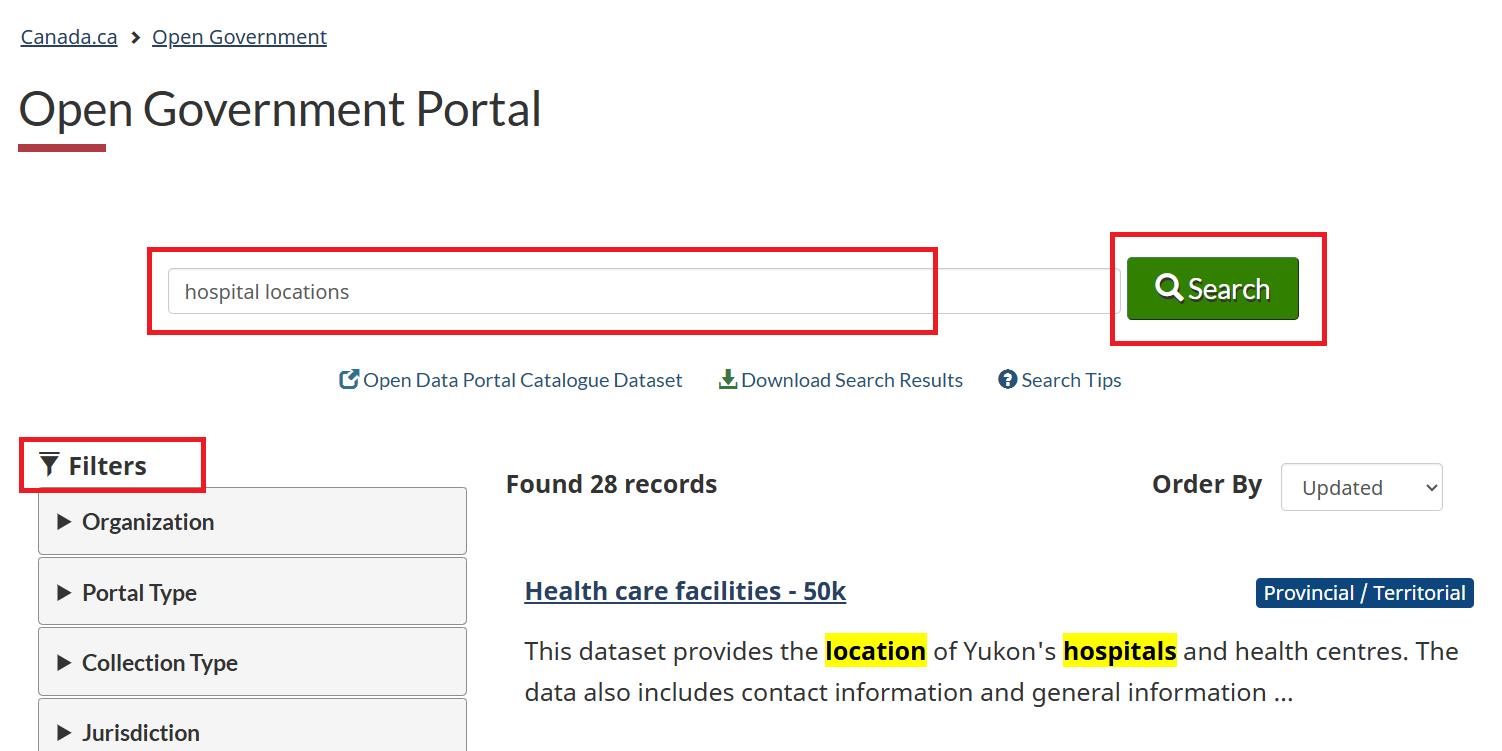
\includegraphics[width=0.9\linewidth,height=\textheight,keepaspectratio]{references/data-sources/../../assets/images/data11/open3.png}
\end{center}

To explore a specific dataset, click its title. This will take you to a
page with more information about the dataset, including its description,
format options, and download links. For example, if you click on the
``Health care facilities - 50k'' dataset, you will find detailed
information about the location of Yukon's hospitals and health centres.

\begin{center}
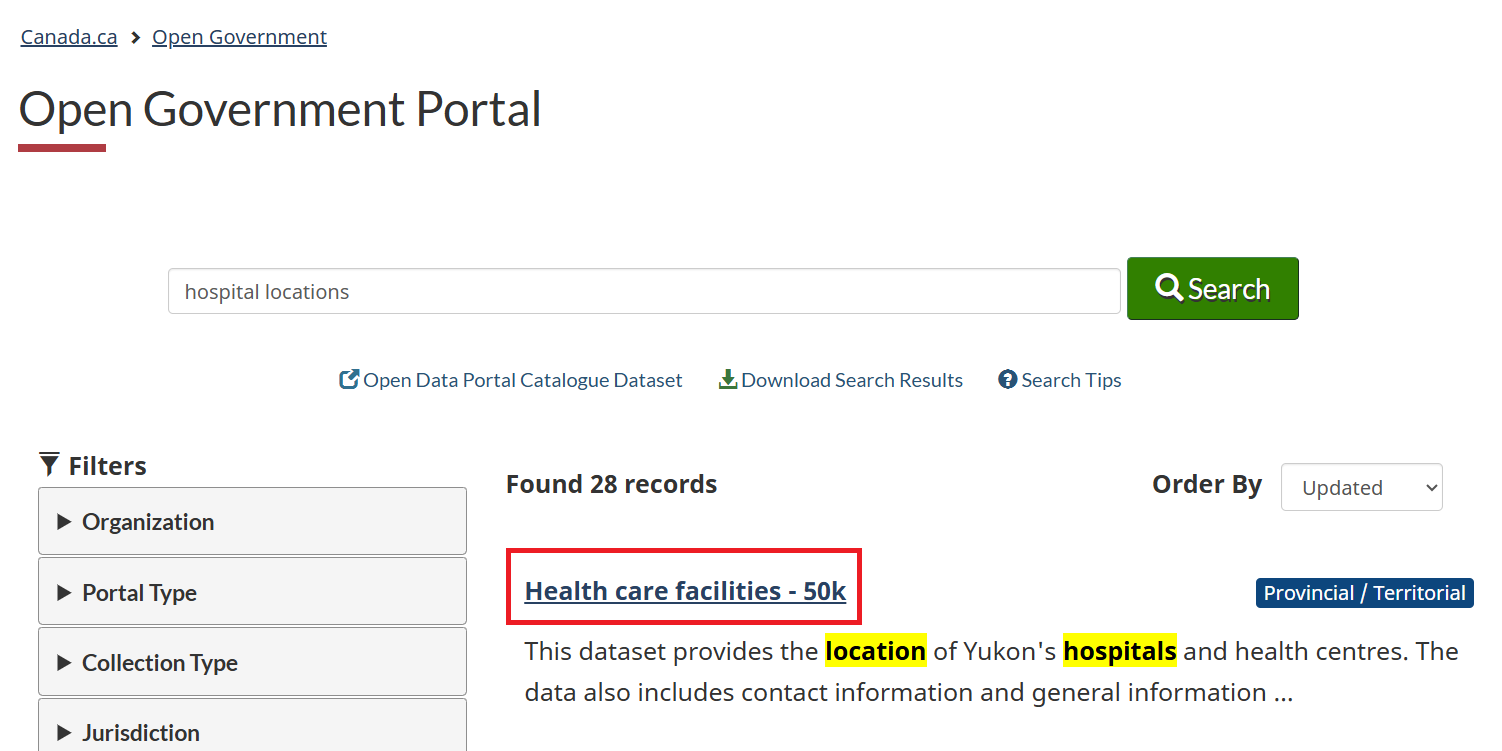
\includegraphics[width=0.9\linewidth,height=\textheight,keepaspectratio]{references/data-sources/../../assets/images/data11/open4.png}
\end{center}

\begin{center}
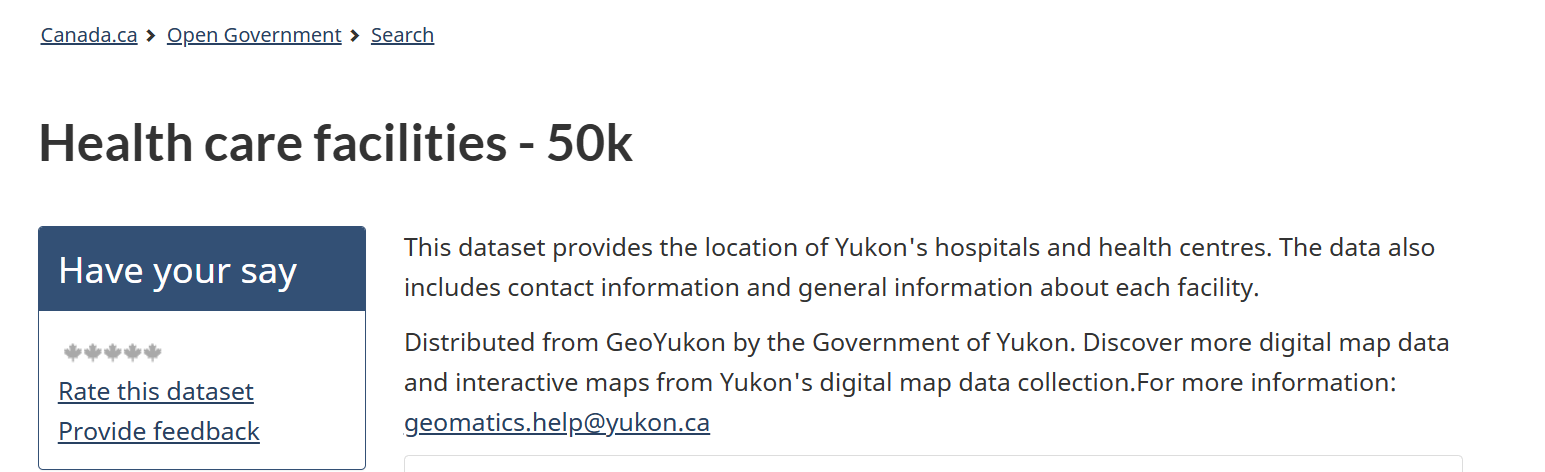
\includegraphics[width=0.9\linewidth,height=\textheight,keepaspectratio]{references/data-sources/../../assets/images/data11/open5.png}
\end{center}

Under the \texttt{Data\ and\ Resources} tab, you can find the available
formats for downloading the location of Yukon's hospitals and health
centres.

\begin{center}
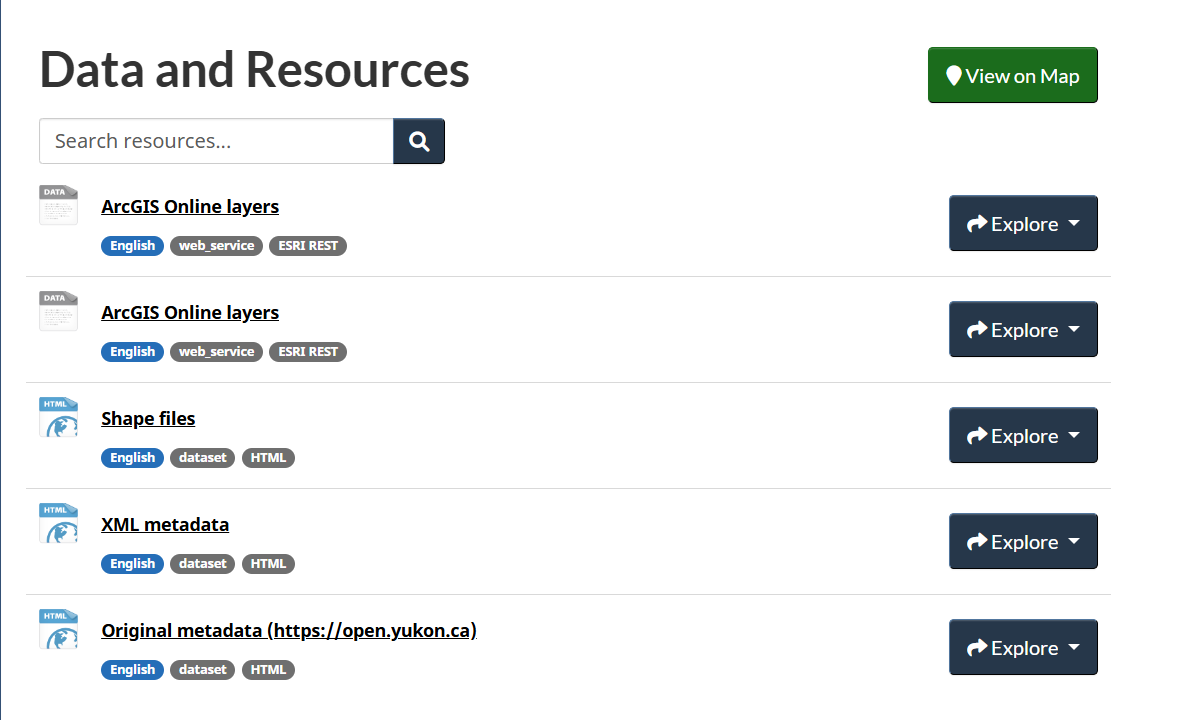
\includegraphics[width=0.9\linewidth,height=\textheight,keepaspectratio]{references/data-sources/../../assets/images/data11/open6.png}
\end{center}

Similarly, say we are interested in ``opioid use'' and want to find open
data related to that topic. We can enter ``opioid use'' into the search
bar and filter by \texttt{Open\ data}:

\begin{center}
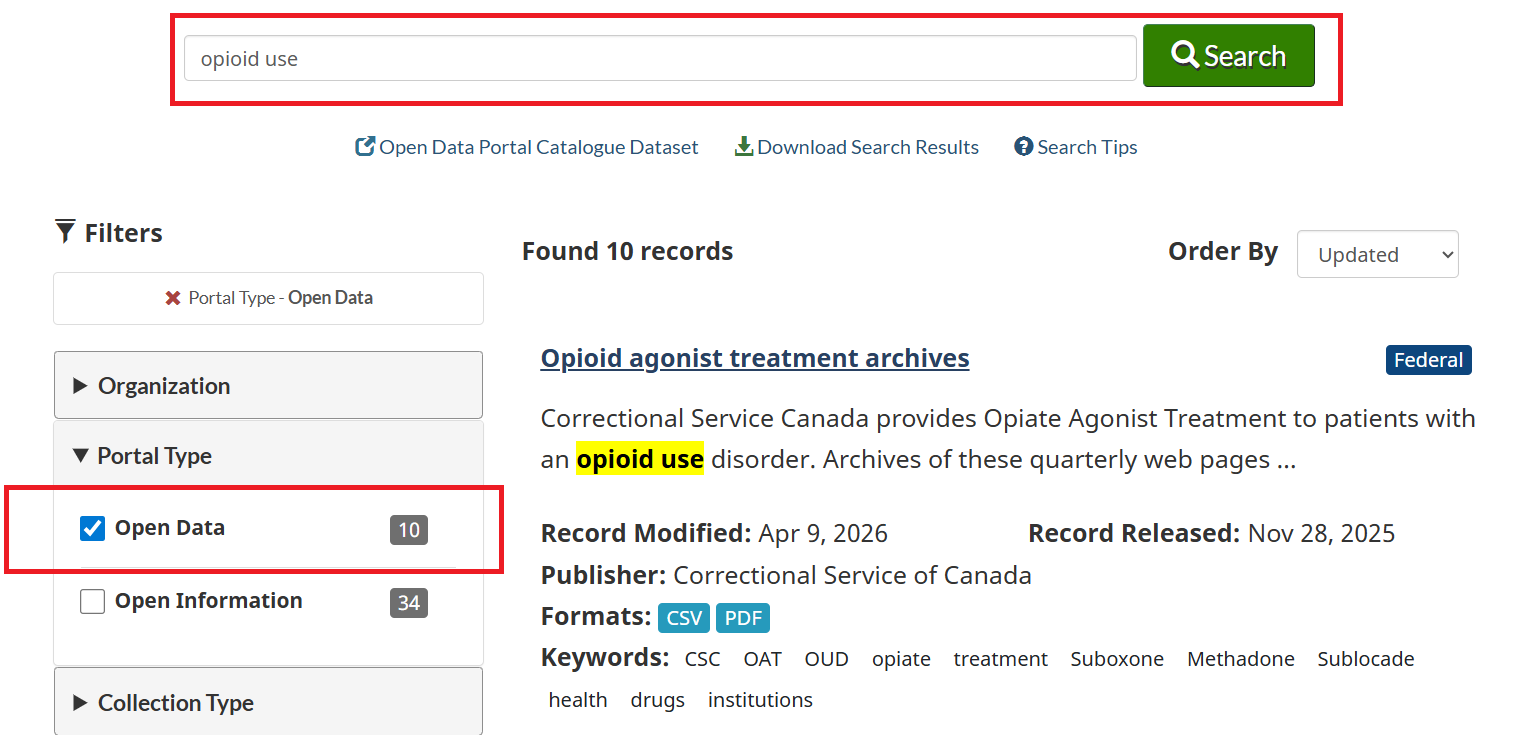
\includegraphics[width=0.9\linewidth,height=\textheight,keepaspectratio]{references/data-sources/../../assets/images/data11/open7.png}
\end{center}

To explore the data on opioid agonist treatment, we can click the
dataset title. This will take us to a page with more information about
the dataset, including its description, format options, and download
links.

\begin{center}
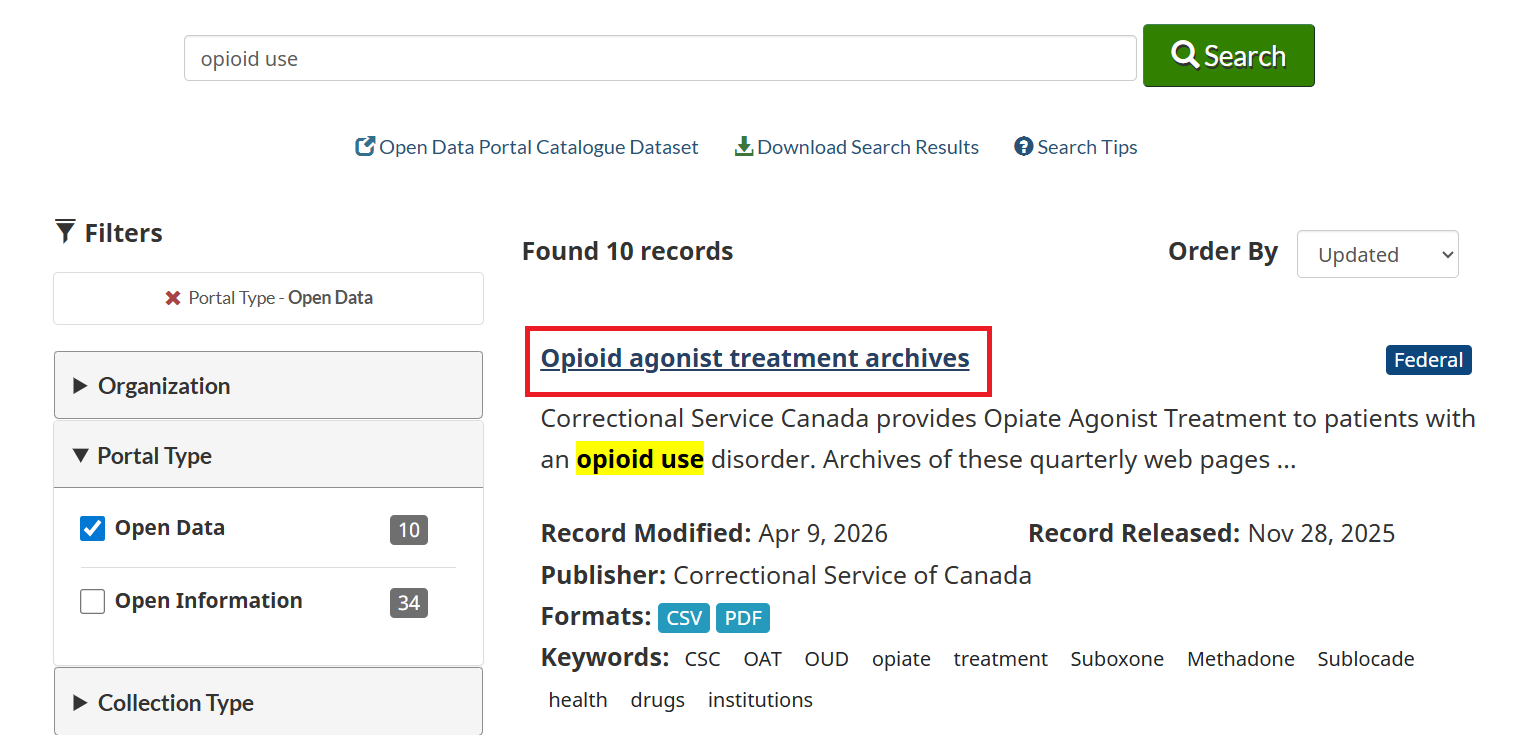
\includegraphics[width=0.9\linewidth,height=\textheight,keepaspectratio]{references/data-sources/../../assets/images/data11/open8.png}
\end{center}

\begin{center}
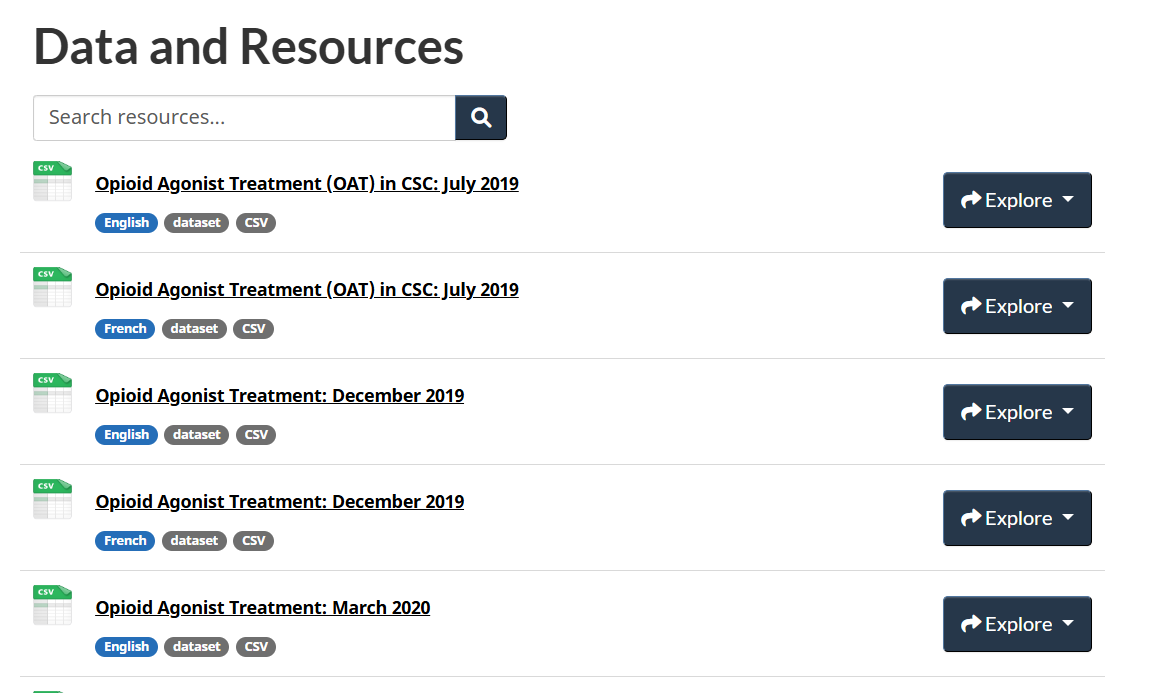
\includegraphics[width=0.9\linewidth,height=\textheight,keepaspectratio]{references/data-sources/../../assets/images/data11/open9.png}
\end{center}

\chapter*{BC Data Catalogue}\label{bc-data-catalogue}
\addcontentsline{toc}{chapter}{BC Data Catalogue}

\markboth{BC Data Catalogue}{BC Data Catalogue}

The British Columbia Data Catalogue is a central hub provided by the
Government of British Columbia (BC). Its primary purpose is to provide
public access to thousands of datasets managed by the provincial
government and its partners. Essentially, it is a digital library
designed to make government information transparent and usable for
citizens, researchers, and developers.

\begin{center}

\includegraphics[width=0.9\linewidth,height=\textheight,keepaspectratio]{references/data-sources/../../assets/images/data12/bc1.png}
\end{center}

\marginnote{\begin{footnotesize}

\href{https://catalogue.data.gov.bc.ca/}{British Columbia Data
Catalogue}

\end{footnotesize}}

\subsection*{Search for Data}\label{search-for-data}
\addcontentsline{toc}{subsection}{Search for Data}

To search for data, you can use the search bar on the BC Data Catalogue
homepage. For example, if you are interested in finding data on
``cancer'', you can enter that term in the search bar and click the
search icon.

\marginnote{\begin{footnotesize}

\href{https://catalogue.data.gov.bc.ca/datasets}{Search Data Catalogue}

\end{footnotesize}}

\begin{center}
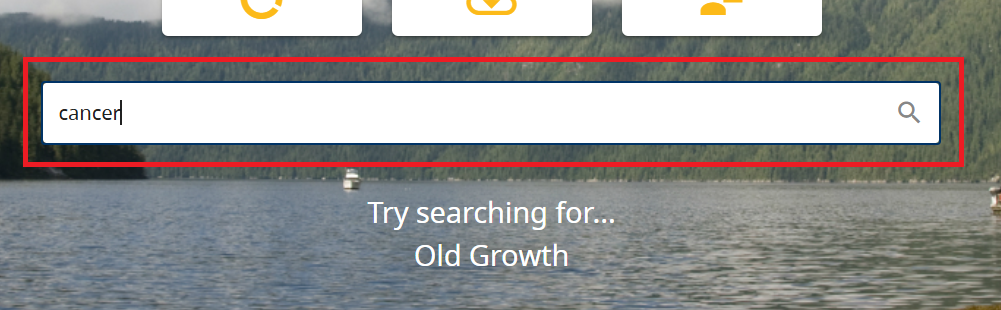
\includegraphics[width=0.9\linewidth,height=\textheight,keepaspectratio]{references/data-sources/../../assets/images/data12/bc2.png}
\end{center}

\begin{center}
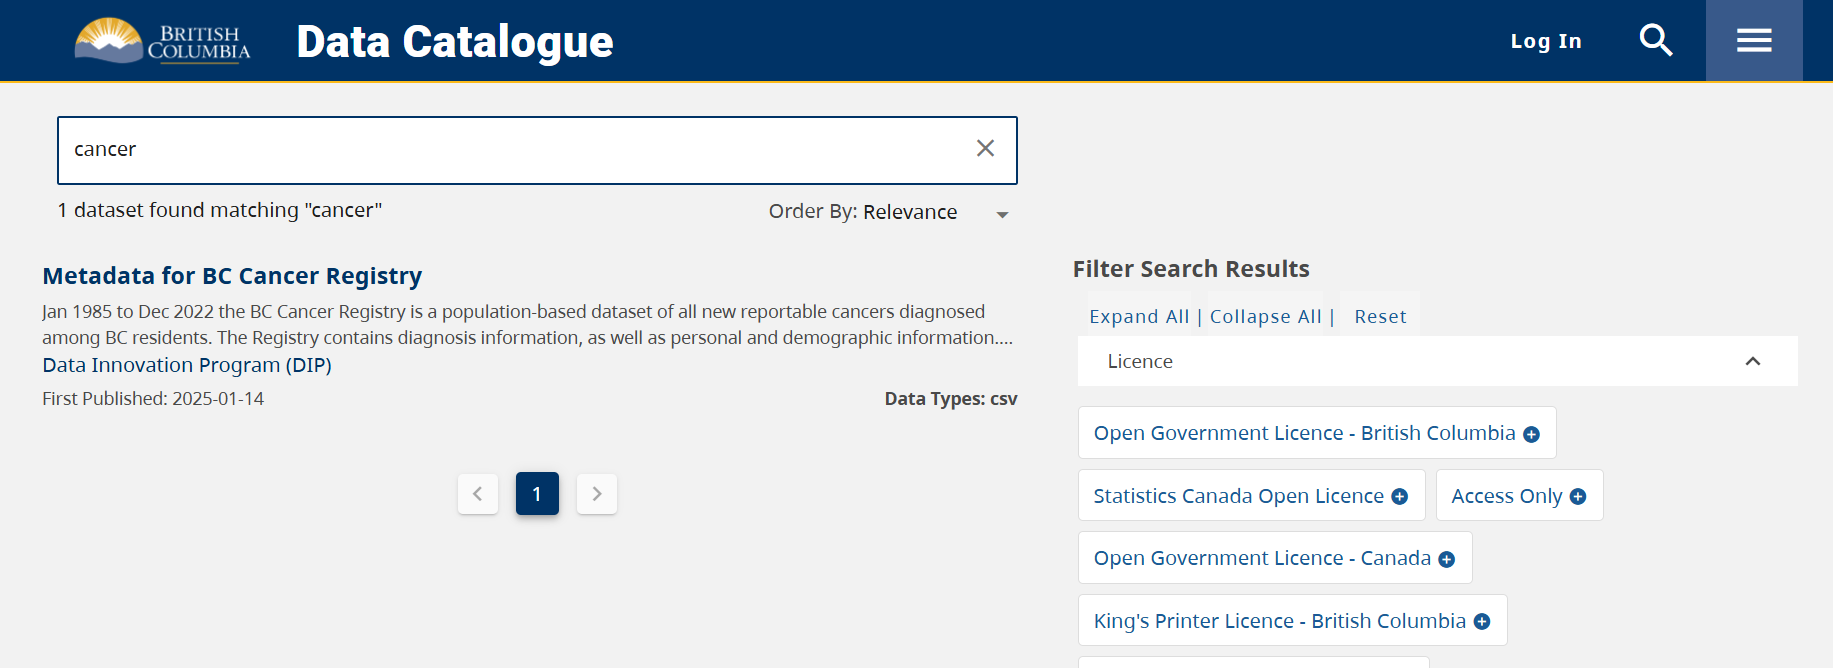
\includegraphics[width=1\linewidth,height=\textheight,keepaspectratio]{references/data-sources/../../assets/images/data12/bc3.png}
\end{center}

Similarly, say we are interested in ``COVID-19'' and want to find open
data related to that topic. We can enter ``covid'' into the search bar:

\begin{center}
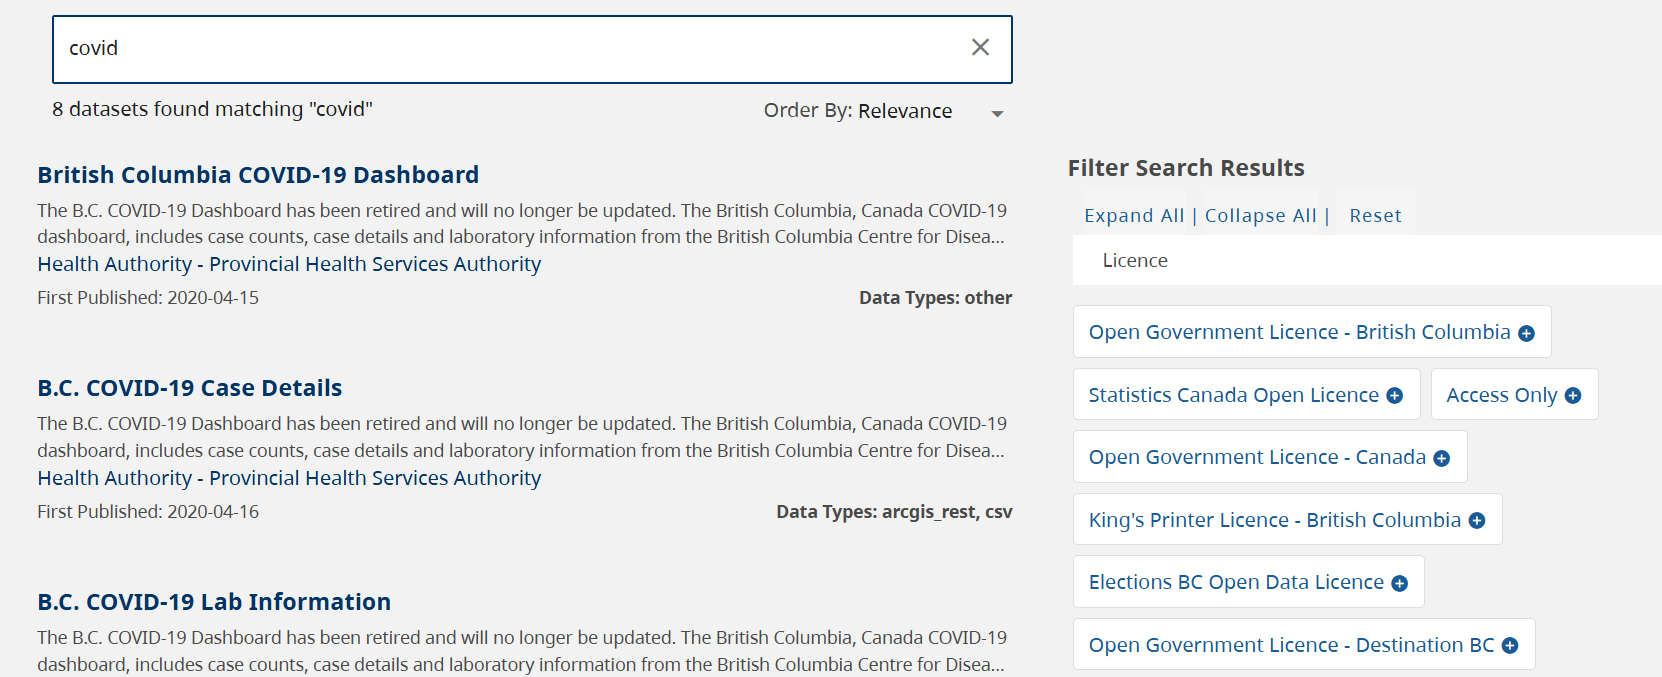
\includegraphics[width=1\linewidth,height=\textheight,keepaspectratio]{references/data-sources/../../assets/images/data12/bc4.png}
\end{center}

You can filter your search by license, format, group, and so on:

\begin{center}
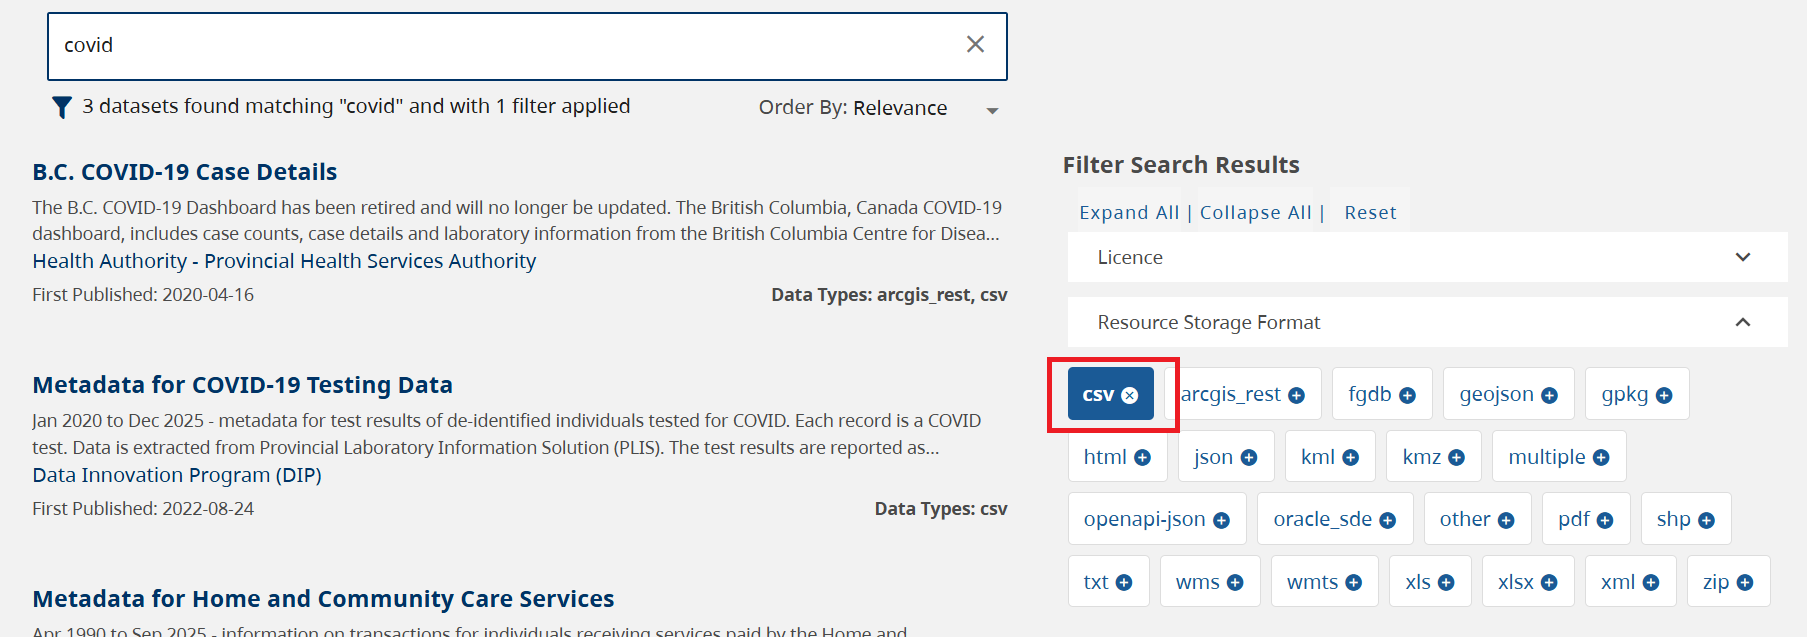
\includegraphics[width=1\linewidth,height=\textheight,keepaspectratio]{references/data-sources/../../assets/images/data12/bc5.png}
\end{center}

Let's explore the ``COVID-19 Case Details'' dataset. To do that, we can
click the dataset title. This will take us to a page with more
information about the dataset, including its description and related
links.

\begin{center}
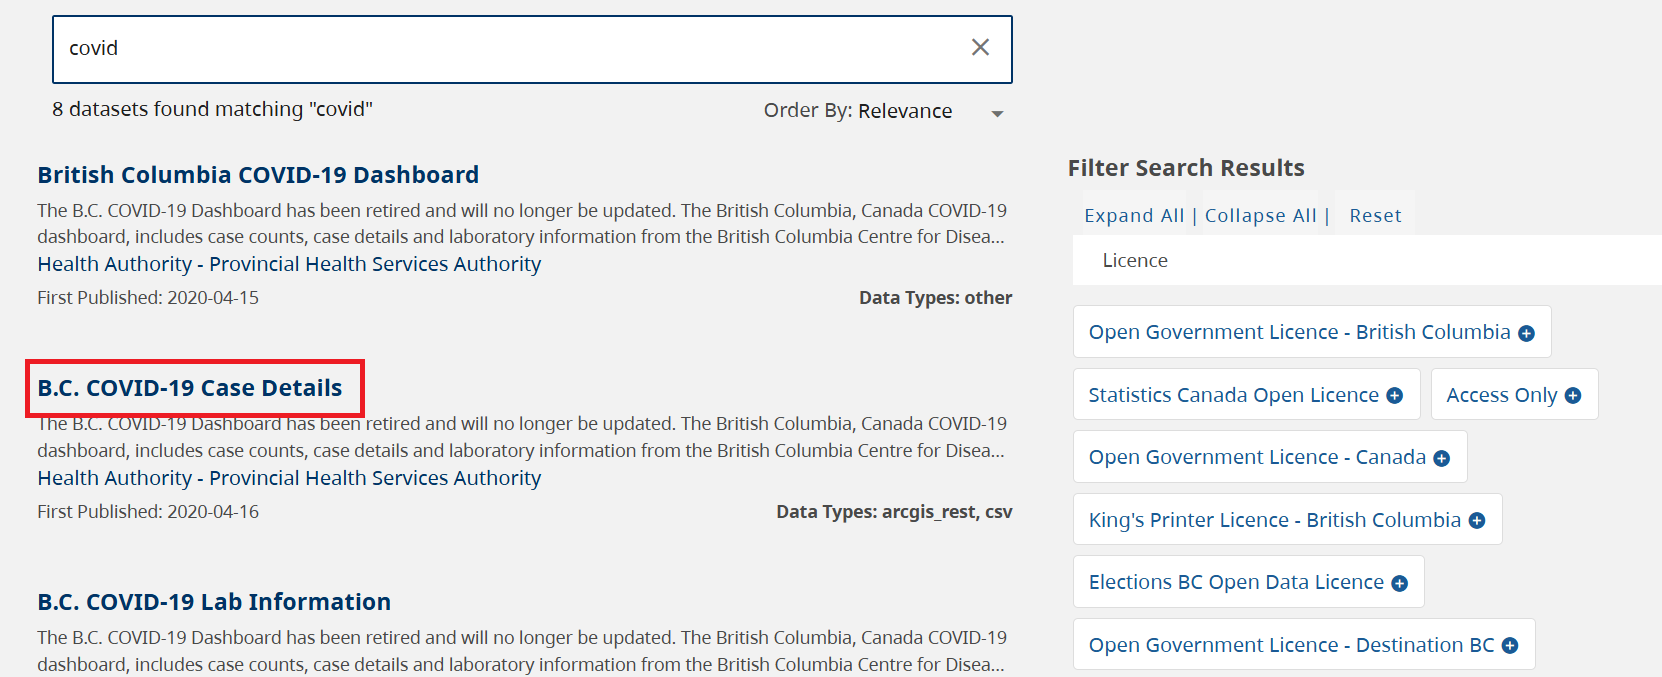
\includegraphics[width=1\linewidth,height=\textheight,keepaspectratio]{references/data-sources/../../assets/images/data12/bc6.png}
\end{center}

You will find information on COVID-19 case details as well as a link to
download the data:

\begin{center}
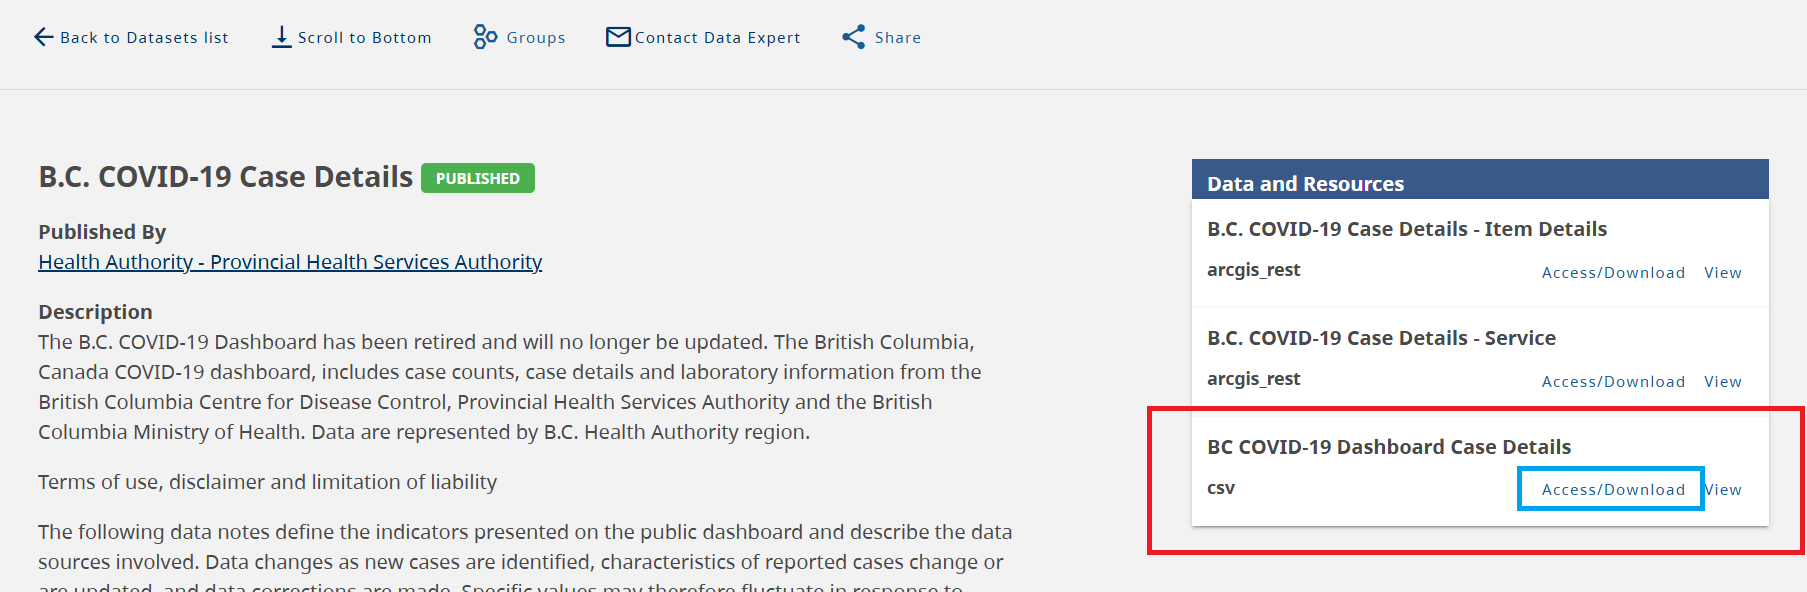
\includegraphics[width=1\linewidth,height=\textheight,keepaspectratio]{references/data-sources/../../assets/images/data12/bc7.png}
\end{center}

To download the dataset, right-click on the \texttt{Access/Download}
link and select \texttt{Save\ link\ as...}. This will allow you to save
the dataset to your computer.

\begin{center}
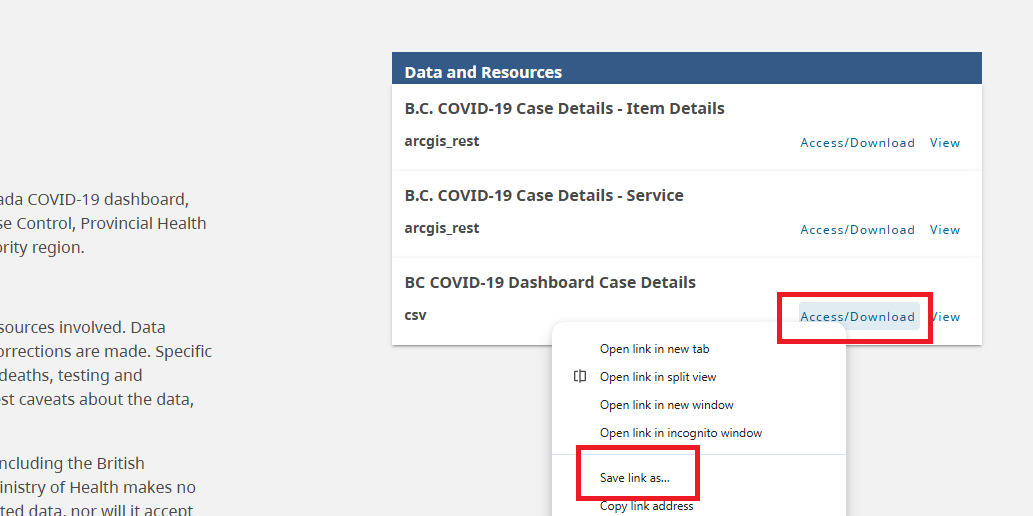
\includegraphics[width=1\linewidth,height=\textheight,keepaspectratio]{references/data-sources/../../assets/images/data12/bc8.png}
\end{center}

\begin{center}
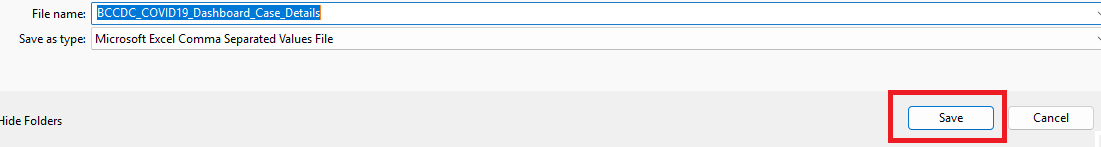
\includegraphics[width=0.9\linewidth,height=\textheight,keepaspectratio]{references/data-sources/../../assets/images/data12/bc9.png}
\end{center}

After downloading, you can open the data in Excel, Google Sheets, or any
statistical software. The data is structured in a tabular format, with
each row representing an individual case and each column representing
different variables.

\begin{center}
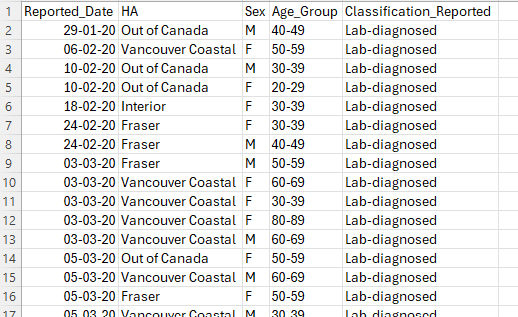
\includegraphics[width=0.9\linewidth,height=\textheight,keepaspectratio]{references/data-sources/../../assets/images/data12/bc10.png}
\end{center}

To learn more about BC Data Catalogue, click on the three bars on the
right side of the page:

\begin{center}
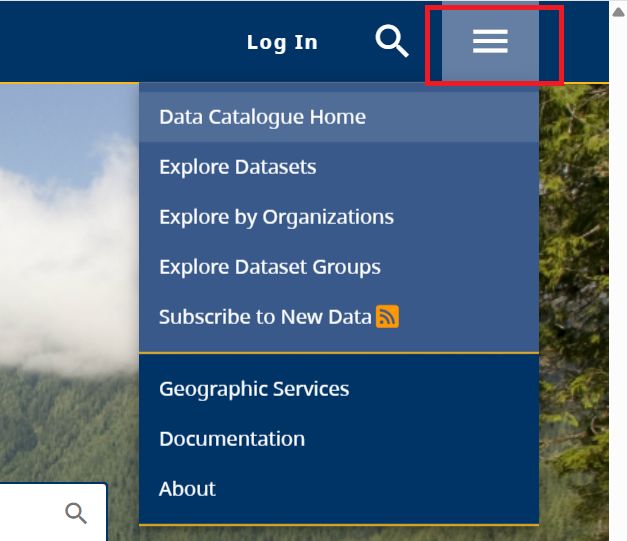
\includegraphics[width=0.8\linewidth,height=\textheight,keepaspectratio]{references/data-sources/../../assets/images/data12/bc11.png}
\end{center}




\end{document}
